\documentclass[twoside]{book}

% Packages required by doxygen
\usepackage{fixltx2e}
\usepackage{calc}
\usepackage{doxygen}
\usepackage{graphicx}
\usepackage[utf8]{inputenc}
\usepackage{makeidx}
\usepackage{multicol}
\usepackage{multirow}
\PassOptionsToPackage{warn}{textcomp}
\usepackage{textcomp}
\usepackage[nointegrals]{wasysym}
\usepackage[table]{xcolor}

% Font selection
\usepackage[T1]{fontenc}
\usepackage{mathptmx}
\usepackage[scaled=.90]{helvet}
\usepackage{courier}
\usepackage{amssymb}
\usepackage{sectsty}
\renewcommand{\familydefault}{\sfdefault}
\allsectionsfont{%
  \fontseries{bc}\selectfont%
  \color{darkgray}%
}
\renewcommand{\DoxyLabelFont}{%
  \fontseries{bc}\selectfont%
  \color{darkgray}%
}
\newcommand{\+}{\discretionary{\mbox{\scriptsize$\hookleftarrow$}}{}{}}

% Page & text layout
\usepackage{geometry}
\geometry{%
  a4paper,%
  top=2.5cm,%
  bottom=2.5cm,%
  left=2.5cm,%
  right=2.5cm%
}
\tolerance=750
\hfuzz=15pt
\hbadness=750
\setlength{\emergencystretch}{15pt}
\setlength{\parindent}{0cm}
\setlength{\parskip}{0.2cm}
\makeatletter
\renewcommand{\paragraph}{%
  \@startsection{paragraph}{4}{0ex}{-1.0ex}{1.0ex}{%
    \normalfont\normalsize\bfseries\SS@parafont%
  }%
}
\renewcommand{\subparagraph}{%
  \@startsection{subparagraph}{5}{0ex}{-1.0ex}{1.0ex}{%
    \normalfont\normalsize\bfseries\SS@subparafont%
  }%
}
\makeatother

% Headers & footers
\usepackage{fancyhdr}
\pagestyle{fancyplain}
\fancyhead[LE]{\fancyplain{}{\bfseries\thepage}}
\fancyhead[CE]{\fancyplain{}{}}
\fancyhead[RE]{\fancyplain{}{\bfseries\leftmark}}
\fancyhead[LO]{\fancyplain{}{\bfseries\rightmark}}
\fancyhead[CO]{\fancyplain{}{}}
\fancyhead[RO]{\fancyplain{}{\bfseries\thepage}}
\fancyfoot[LE]{\fancyplain{}{}}
\fancyfoot[CE]{\fancyplain{}{}}
\fancyfoot[RE]{\fancyplain{}{\bfseries\scriptsize Generated on Sat Feb 27 2016 21\+:36\+:22 for Dbo by Doxygen }}
\fancyfoot[LO]{\fancyplain{}{\bfseries\scriptsize Generated on Sat Feb 27 2016 21\+:36\+:22 for Dbo by Doxygen }}
\fancyfoot[CO]{\fancyplain{}{}}
\fancyfoot[RO]{\fancyplain{}{}}
\renewcommand{\footrulewidth}{0.4pt}
\renewcommand{\chaptermark}[1]{%
  \markboth{#1}{}%
}
\renewcommand{\sectionmark}[1]{%
  \markright{\thesection\ #1}%
}

% Indices & bibliography
\usepackage{natbib}
\usepackage[titles]{tocloft}
\setcounter{tocdepth}{3}
\setcounter{secnumdepth}{5}
\makeindex

% Hyperlinks (required, but should be loaded last)
\usepackage{ifpdf}
\ifpdf
  \usepackage[pdftex,pagebackref=true]{hyperref}
\else
  \usepackage[ps2pdf,pagebackref=true]{hyperref}
\fi
\hypersetup{%
  colorlinks=true,%
  linkcolor=blue,%
  citecolor=blue,%
  unicode%
}

% Custom commands
\newcommand{\clearemptydoublepage}{%
  \newpage{\pagestyle{empty}\cleardoublepage}%
}


%===== C O N T E N T S =====

\begin{document}

% Titlepage & ToC
\hypersetup{pageanchor=false,
             bookmarks=true,
             bookmarksnumbered=true,
             pdfencoding=unicode
            }
\pagenumbering{roman}
\begin{titlepage}
\vspace*{7cm}
\begin{center}%
{\Large Dbo }\\
\vspace*{1cm}
{\large Generated by Doxygen 1.8.7}\\
\vspace*{0.5cm}
{\small Sat Feb 27 2016 21:36:22}\\
\end{center}
\end{titlepage}
\clearemptydoublepage
\tableofcontents
\clearemptydoublepage
\pagenumbering{arabic}
\hypersetup{pageanchor=true}

%--- Begin generated contents ---
\chapter{Namespace Index}
\section{Namespace List}
Here is a list of all namespaces with brief descriptions\+:\begin{DoxyCompactList}
\item\contentsline{section}{\hyperlink{namespacedbo}{dbo} }{\pageref{namespacedbo}}{}
\item\contentsline{section}{\hyperlink{namespacedbo_1_1action}{dbo\+::action} }{\pageref{namespacedbo_1_1action}}{}
\item\contentsline{section}{\hyperlink{namespacedbo_1_1fk}{dbo\+::fk} }{\pageref{namespacedbo_1_1fk}}{}
\item\contentsline{section}{\hyperlink{namespacedbo_1_1mapping}{dbo\+::mapping} }{\pageref{namespacedbo_1_1mapping}}{}
\item\contentsline{section}{\hyperlink{namespacedbo_1_1opt}{dbo\+::opt} }{\pageref{namespacedbo_1_1opt}}{}
\item\contentsline{section}{\hyperlink{namespacedbo_1_1stmt}{dbo\+::stmt} }{\pageref{namespacedbo_1_1stmt}}{}
\item\contentsline{section}{\hyperlink{namespacedbo_1_1traits}{dbo\+::traits} }{\pageref{namespacedbo_1_1traits}}{}
\end{DoxyCompactList}

\chapter{Hierarchical Index}
\section{Class Hierarchy}
This inheritance list is sorted roughly, but not completely, alphabetically\+:\begin{DoxyCompactList}
\item \contentsline{section}{dbo\+:\+:Action\+Option}{\pageref{classdbo_1_1_action_option}}{}
\item \contentsline{section}{dbo\+:\+:stmt\+:\+:Bulk\+Statement\+:\+:Buffer}{\pageref{structdbo_1_1stmt_1_1_bulk_statement_1_1_buffer}}{}
\item \contentsline{section}{dbo\+:\+:action\+:\+:Bulk\+Insert$<$ C $>$}{\pageref{classdbo_1_1action_1_1_bulk_insert}}{}
\item \contentsline{section}{dbo\+:\+:collection$<$ C $>$}{\pageref{classdbo_1_1collection}}{}
\item \contentsline{section}{dbo\+:\+:mapping\+:\+:Collection\+Ref$<$ T $>$}{\pageref{classdbo_1_1mapping_1_1_collection_ref}}{}
\item \contentsline{section}{dbo\+:\+:connection}{\pageref{classdbo_1_1connection}}{}
\item \contentsline{section}{dbo\+\_\+default\+\_\+traits}{\pageref{structdbo__default__traits}}{}
\begin{DoxyCompactList}
\item \contentsline{section}{dbo\+:\+:traits\+:\+:dbo\+\_\+traits$<$ C $>$}{\pageref{structdbo_1_1traits_1_1dbo__traits}}{}
\end{DoxyCompactList}
\item \contentsline{section}{dbo\+:\+:action\+:\+:Delete$<$ C $>$}{\pageref{classdbo_1_1action_1_1_delete}}{}
\item \contentsline{section}{dbo\+:\+:mapping\+:\+:Field\+Info}{\pageref{classdbo_1_1mapping_1_1_field_info}}{}
\item \contentsline{section}{dbo\+:\+:mapping\+:\+:Field\+Ref$<$ T $>$}{\pageref{classdbo_1_1mapping_1_1_field_ref}}{}
\item \contentsline{section}{dbo\+:\+:Foreign\+Key\+Constraint}{\pageref{classdbo_1_1_foreign_key_constraint}}{}
\item \contentsline{section}{dbo\+:\+:action\+:\+:Init\+Schema}{\pageref{classdbo_1_1action_1_1_init_schema}}{}
\item \contentsline{section}{dbo\+:\+:action\+:\+:Insert$<$ C $>$}{\pageref{classdbo_1_1action_1_1_insert}}{}
\item \contentsline{section}{is\+\_\+raw\+\_\+string$<$ Type $>$}{\pageref{structis__raw__string}}{}
\item iterator\begin{DoxyCompactList}
\item \contentsline{section}{dbo\+:\+:collection$<$ C $>$\+:\+:iterator}{\pageref{classdbo_1_1collection_1_1iterator}}{}
\end{DoxyCompactList}
\item \contentsline{section}{dbo\+:\+:mapping\+:\+:Join\+Id}{\pageref{structdbo_1_1mapping_1_1_join_id}}{}
\item \contentsline{section}{dbo\+:\+:action\+:\+:Load\+Db$<$ C $>$}{\pageref{classdbo_1_1action_1_1_load_db}}{}
\item \contentsline{section}{dbo\+:\+:mapping\+:\+:Mapping\+Info}{\pageref{classdbo_1_1mapping_1_1_mapping_info}}{}
\begin{DoxyCompactList}
\item \contentsline{section}{dbo\+:\+:mapping\+:\+:Mapping$<$ T $>$}{\pageref{classdbo_1_1mapping_1_1_mapping}}{}
\item \contentsline{section}{dbo\+:\+:mapping\+:\+:Mapping$<$ C $>$}{\pageref{classdbo_1_1mapping_1_1_mapping}}{}
\end{DoxyCompactList}
\item \contentsline{section}{dbo\+:\+:ptr$<$ C $>$\+:\+:Ptr}{\pageref{structdbo_1_1ptr_1_1_ptr}}{}
\item \contentsline{section}{dbo\+:\+:ptr\+\_\+base}{\pageref{classdbo_1_1ptr__base}}{}
\begin{DoxyCompactList}
\item \contentsline{section}{dbo\+:\+:ptr$<$ C $>$}{\pageref{classdbo_1_1ptr}}{}
\end{DoxyCompactList}
\item \contentsline{section}{dbo\+:\+:mapping\+:\+:Ptr\+Ref$<$ T $>$}{\pageref{classdbo_1_1mapping_1_1_ptr_ref}}{}
\item \contentsline{section}{dbo\+:\+:query}{\pageref{classdbo_1_1query}}{}
\item runtime\+\_\+error\begin{DoxyCompactList}
\item \contentsline{section}{dbo\+:\+:Exception}{\pageref{classdbo_1_1_exception}}{}
\end{DoxyCompactList}
\item \contentsline{section}{dbo\+:\+:action\+:\+:Select\+By\+Id$<$ C $>$}{\pageref{classdbo_1_1action_1_1_select_by_id}}{}
\item \contentsline{section}{dbo\+:\+:mapping\+:\+:Set\+Info}{\pageref{structdbo_1_1mapping_1_1_set_info}}{}
\item \contentsline{section}{dbo\+:\+:traits\+:\+:sql\+\_\+value\+\_\+traits$<$ V, Enable $>$}{\pageref{structdbo_1_1traits_1_1sql__value__traits}}{}
\item \contentsline{section}{dbo\+:\+:traits\+:\+:sql\+\_\+value\+\_\+traits$<$ bool, void $>$}{\pageref{structdbo_1_1traits_1_1sql__value__traits_3_01bool_00_01void_01_4}}{}
\item \contentsline{section}{dbo\+:\+:traits\+:\+:sql\+\_\+value\+\_\+traits$<$ boost\+:\+:gregorian\+:\+:date, void $>$}{\pageref{structdbo_1_1traits_1_1sql__value__traits_3_01boost_1_1gregorian_1_1date_00_01void_01_4}}{}
\item \contentsline{section}{dbo\+:\+:traits\+:\+:sql\+\_\+value\+\_\+traits$<$ boost\+:\+:optional$<$ T $>$, void $>$}{\pageref{structdbo_1_1traits_1_1sql__value__traits_3_01boost_1_1optional_3_01_t_01_4_00_01void_01_4}}{}
\item \contentsline{section}{dbo\+:\+:traits\+:\+:sql\+\_\+value\+\_\+traits$<$ boost\+:\+:posix\+\_\+time\+:\+:ptime, void $>$}{\pageref{structdbo_1_1traits_1_1sql__value__traits_3_01boost_1_1posix__time_1_1ptime_00_01void_01_4}}{}
\item \contentsline{section}{dbo\+:\+:traits\+:\+:sql\+\_\+value\+\_\+traits$<$ boost\+:\+:posix\+\_\+time\+:\+:time\+\_\+duration, void $>$}{\pageref{structdbo_1_1traits_1_1sql__value__traits_3_01boost_1_1posix__time_1_1time__duration_00_01void_01_4}}{}
\item \contentsline{section}{dbo\+:\+:traits\+:\+:sql\+\_\+value\+\_\+traits$<$ double, void $>$}{\pageref{structdbo_1_1traits_1_1sql__value__traits_3_01double_00_01void_01_4}}{}
\item \contentsline{section}{dbo\+:\+:traits\+:\+:sql\+\_\+value\+\_\+traits$<$ float, void $>$}{\pageref{structdbo_1_1traits_1_1sql__value__traits_3_01float_00_01void_01_4}}{}
\item \contentsline{section}{dbo\+:\+:traits\+:\+:sql\+\_\+value\+\_\+traits$<$ int $>$}{\pageref{structdbo_1_1traits_1_1sql__value__traits}}{}
\begin{DoxyCompactList}
\item \contentsline{section}{dbo\+:\+:traits\+:\+:sql\+\_\+value\+\_\+traits$<$ Enum, typename boost\+:\+:enable\+\_\+if$<$ boost\+:\+:is\+\_\+enum$<$ Enum $>$ $>$\+:\+:type $>$}{\pageref{structdbo_1_1traits_1_1sql__value__traits_3_01_enum_00_01typename_01boost_1_1enable__if_3_01boosf3db7d431a3cc6684d99d55c76c69c74}}{}
\end{DoxyCompactList}
\item \contentsline{section}{dbo\+:\+:traits\+:\+:sql\+\_\+value\+\_\+traits$<$ int, void $>$}{\pageref{structdbo_1_1traits_1_1sql__value__traits_3_01int_00_01void_01_4}}{}
\item \contentsline{section}{dbo\+:\+:traits\+:\+:sql\+\_\+value\+\_\+traits$<$ long long, void $>$}{\pageref{structdbo_1_1traits_1_1sql__value__traits_3_01long_01long_00_01void_01_4}}{}
\item \contentsline{section}{dbo\+:\+:traits\+:\+:sql\+\_\+value\+\_\+traits$<$ long, void $>$}{\pageref{structdbo_1_1traits_1_1sql__value__traits_3_01long_00_01void_01_4}}{}
\item \contentsline{section}{dbo\+:\+:traits\+:\+:sql\+\_\+value\+\_\+traits$<$ short, void $>$}{\pageref{structdbo_1_1traits_1_1sql__value__traits_3_01short_00_01void_01_4}}{}
\item \contentsline{section}{dbo\+:\+:traits\+:\+:sql\+\_\+value\+\_\+traits$<$ size\+\_\+t, void $>$}{\pageref{structdbo_1_1traits_1_1sql__value__traits_3_01size__t_00_01void_01_4}}{}
\item \contentsline{section}{dbo\+:\+:traits\+:\+:sql\+\_\+value\+\_\+traits$<$ std\+:\+:string $>$}{\pageref{structdbo_1_1traits_1_1sql__value__traits}}{}
\begin{DoxyCompactList}
\item \contentsline{section}{dbo\+:\+:traits\+:\+:sql\+\_\+value\+\_\+traits$<$ Type, typename boost\+:\+:enable\+\_\+if$<$ is\+\_\+raw\+\_\+string$<$ Type $>$ $>$\+:\+:type $>$}{\pageref{structdbo_1_1traits_1_1sql__value__traits_3_01_type_00_01typename_01boost_1_1enable__if_3_01is__aa5117fa5e949e5d70ea0660f0e85288}}{}
\end{DoxyCompactList}
\item \contentsline{section}{dbo\+:\+:traits\+:\+:sql\+\_\+value\+\_\+traits$<$ std\+:\+:string, void $>$}{\pageref{structdbo_1_1traits_1_1sql__value__traits_3_01std_1_1string_00_01void_01_4}}{}
\item \contentsline{section}{dbo\+:\+:traits\+:\+:sql\+\_\+value\+\_\+traits$<$ std\+:\+:vector$<$ unsigned char $>$, void $>$}{\pageref{structdbo_1_1traits_1_1sql__value__traits_3_01std_1_1vector_3_01unsigned_01char_01_4_00_01void_01_4}}{}
\item \contentsline{section}{dbo\+:\+:traits\+:\+:Sql\+Postgres\+Types}{\pageref{classdbo_1_1traits_1_1_sql_postgres_types}}{}
\item \contentsline{section}{dbo\+:\+:stmt\+:\+:Statement}{\pageref{classdbo_1_1stmt_1_1_statement}}{}
\begin{DoxyCompactList}
\item \contentsline{section}{dbo\+:\+:stmt\+:\+:Bulk\+Statement}{\pageref{classdbo_1_1stmt_1_1_bulk_statement}}{}
\item \contentsline{section}{dbo\+:\+:stmt\+:\+:Prepared\+Statement}{\pageref{classdbo_1_1stmt_1_1_prepared_statement}}{}
\end{DoxyCompactList}
\item \contentsline{section}{dbo\+:\+:transaction}{\pageref{classdbo_1_1transaction}}{}
\item \contentsline{section}{dbo\+:\+:connection\+:\+:typecomp}{\pageref{structdbo_1_1connection_1_1typecomp}}{}
\item \contentsline{section}{dbo\+:\+:action\+:\+:Update$<$ C $>$}{\pageref{classdbo_1_1action_1_1_update}}{}
\end{DoxyCompactList}

\chapter{Class Index}
\section{Class List}
Here are the classes, structs, unions and interfaces with brief descriptions\+:\begin{DoxyCompactList}
\item\contentsline{section}{\hyperlink{classdbo_1_1_action_option}{dbo\+::\+Action\+Option} }{\pageref{classdbo_1_1_action_option}}{}
\item\contentsline{section}{\hyperlink{structdbo_1_1stmt_1_1_bulk_statement_1_1_buffer}{dbo\+::stmt\+::\+Bulk\+Statement\+::\+Buffer} }{\pageref{structdbo_1_1stmt_1_1_bulk_statement_1_1_buffer}}{}
\item\contentsline{section}{\hyperlink{classdbo_1_1action_1_1_bulk_insert}{dbo\+::action\+::\+Bulk\+Insert$<$ C $>$} }{\pageref{classdbo_1_1action_1_1_bulk_insert}}{}
\item\contentsline{section}{\hyperlink{classdbo_1_1stmt_1_1_bulk_statement}{dbo\+::stmt\+::\+Bulk\+Statement} }{\pageref{classdbo_1_1stmt_1_1_bulk_statement}}{}
\item\contentsline{section}{\hyperlink{classdbo_1_1collection}{dbo\+::collection$<$ C $>$} }{\pageref{classdbo_1_1collection}}{}
\item\contentsline{section}{\hyperlink{classdbo_1_1mapping_1_1_collection_ref}{dbo\+::mapping\+::\+Collection\+Ref$<$ T $>$} }{\pageref{classdbo_1_1mapping_1_1_collection_ref}}{}
\item\contentsline{section}{\hyperlink{classdbo_1_1connection}{dbo\+::connection} }{\pageref{classdbo_1_1connection}}{}
\item\contentsline{section}{\hyperlink{structdbo__default__traits}{dbo\+\_\+default\+\_\+traits} \\*Default traits for a class mapped with \%Dbo }{\pageref{structdbo__default__traits}}{}
\item\contentsline{section}{\hyperlink{structdbo_1_1traits_1_1dbo__traits}{dbo\+::traits\+::dbo\+\_\+traits$<$ C $>$} \\*Traits for a class mapped with \%Dbo }{\pageref{structdbo_1_1traits_1_1dbo__traits}}{}
\item\contentsline{section}{\hyperlink{classdbo_1_1action_1_1_delete}{dbo\+::action\+::\+Delete$<$ C $>$} }{\pageref{classdbo_1_1action_1_1_delete}}{}
\item\contentsline{section}{\hyperlink{classdbo_1_1_exception}{dbo\+::\+Exception} }{\pageref{classdbo_1_1_exception}}{}
\item\contentsline{section}{\hyperlink{classdbo_1_1mapping_1_1_field_info}{dbo\+::mapping\+::\+Field\+Info} \\*Description of a field }{\pageref{classdbo_1_1mapping_1_1_field_info}}{}
\item\contentsline{section}{\hyperlink{classdbo_1_1mapping_1_1_field_ref}{dbo\+::mapping\+::\+Field\+Ref$<$ T $>$} }{\pageref{classdbo_1_1mapping_1_1_field_ref}}{}
\item\contentsline{section}{\hyperlink{classdbo_1_1_foreign_key_constraint}{dbo\+::\+Foreign\+Key\+Constraint} }{\pageref{classdbo_1_1_foreign_key_constraint}}{}
\item\contentsline{section}{\hyperlink{classdbo_1_1action_1_1_init_schema}{dbo\+::action\+::\+Init\+Schema} }{\pageref{classdbo_1_1action_1_1_init_schema}}{}
\item\contentsline{section}{\hyperlink{classdbo_1_1action_1_1_insert}{dbo\+::action\+::\+Insert$<$ C $>$} }{\pageref{classdbo_1_1action_1_1_insert}}{}
\item\contentsline{section}{\hyperlink{structis__raw__string}{is\+\_\+raw\+\_\+string$<$ Type $>$} }{\pageref{structis__raw__string}}{}
\item\contentsline{section}{\hyperlink{classdbo_1_1collection_1_1iterator}{dbo\+::collection$<$ C $>$\+::iterator} }{\pageref{classdbo_1_1collection_1_1iterator}}{}
\item\contentsline{section}{\hyperlink{structdbo_1_1mapping_1_1_join_id}{dbo\+::mapping\+::\+Join\+Id} }{\pageref{structdbo_1_1mapping_1_1_join_id}}{}
\item\contentsline{section}{\hyperlink{classdbo_1_1action_1_1_load_db}{dbo\+::action\+::\+Load\+Db$<$ C $>$} }{\pageref{classdbo_1_1action_1_1_load_db}}{}
\item\contentsline{section}{\hyperlink{classdbo_1_1mapping_1_1_mapping}{dbo\+::mapping\+::\+Mapping$<$ T $>$} }{\pageref{classdbo_1_1mapping_1_1_mapping}}{}
\item\contentsline{section}{\hyperlink{classdbo_1_1mapping_1_1_mapping_info}{dbo\+::mapping\+::\+Mapping\+Info} }{\pageref{classdbo_1_1mapping_1_1_mapping_info}}{}
\item\contentsline{section}{\hyperlink{classdbo_1_1stmt_1_1_prepared_statement}{dbo\+::stmt\+::\+Prepared\+Statement} }{\pageref{classdbo_1_1stmt_1_1_prepared_statement}}{}
\item\contentsline{section}{\hyperlink{classdbo_1_1ptr}{dbo\+::ptr$<$ C $>$} }{\pageref{classdbo_1_1ptr}}{}
\item\contentsline{section}{\hyperlink{structdbo_1_1ptr_1_1_ptr}{dbo\+::ptr$<$ C $>$\+::\+Ptr} }{\pageref{structdbo_1_1ptr_1_1_ptr}}{}
\item\contentsline{section}{\hyperlink{classdbo_1_1ptr__base}{dbo\+::ptr\+\_\+base} }{\pageref{classdbo_1_1ptr__base}}{}
\item\contentsline{section}{\hyperlink{classdbo_1_1mapping_1_1_ptr_ref}{dbo\+::mapping\+::\+Ptr\+Ref$<$ T $>$} }{\pageref{classdbo_1_1mapping_1_1_ptr_ref}}{}
\item\contentsline{section}{\hyperlink{classdbo_1_1query}{dbo\+::query} }{\pageref{classdbo_1_1query}}{}
\item\contentsline{section}{\hyperlink{classdbo_1_1action_1_1_select_by_id}{dbo\+::action\+::\+Select\+By\+Id$<$ C $>$} }{\pageref{classdbo_1_1action_1_1_select_by_id}}{}
\item\contentsline{section}{\hyperlink{structdbo_1_1mapping_1_1_set_info}{dbo\+::mapping\+::\+Set\+Info} }{\pageref{structdbo_1_1mapping_1_1_set_info}}{}
\item\contentsline{section}{\hyperlink{structdbo_1_1traits_1_1sql__value__traits}{dbo\+::traits\+::sql\+\_\+value\+\_\+traits$<$ V, Enable $>$} \\*Traits class for value types }{\pageref{structdbo_1_1traits_1_1sql__value__traits}}{}
\item\contentsline{section}{\hyperlink{structdbo_1_1traits_1_1sql__value__traits_3_01bool_00_01void_01_4}{dbo\+::traits\+::sql\+\_\+value\+\_\+traits$<$ bool, void $>$} }{\pageref{structdbo_1_1traits_1_1sql__value__traits_3_01bool_00_01void_01_4}}{}
\item\contentsline{section}{\hyperlink{structdbo_1_1traits_1_1sql__value__traits_3_01boost_1_1gregorian_1_1date_00_01void_01_4}{dbo\+::traits\+::sql\+\_\+value\+\_\+traits$<$ boost\+::gregorian\+::date, void $>$} }{\pageref{structdbo_1_1traits_1_1sql__value__traits_3_01boost_1_1gregorian_1_1date_00_01void_01_4}}{}
\item\contentsline{section}{\hyperlink{structdbo_1_1traits_1_1sql__value__traits_3_01boost_1_1optional_3_01_t_01_4_00_01void_01_4}{dbo\+::traits\+::sql\+\_\+value\+\_\+traits$<$ boost\+::optional$<$ T $>$, void $>$} }{\pageref{structdbo_1_1traits_1_1sql__value__traits_3_01boost_1_1optional_3_01_t_01_4_00_01void_01_4}}{}
\item\contentsline{section}{\hyperlink{structdbo_1_1traits_1_1sql__value__traits_3_01boost_1_1posix__time_1_1ptime_00_01void_01_4}{dbo\+::traits\+::sql\+\_\+value\+\_\+traits$<$ boost\+::posix\+\_\+time\+::ptime, void $>$} }{\pageref{structdbo_1_1traits_1_1sql__value__traits_3_01boost_1_1posix__time_1_1ptime_00_01void_01_4}}{}
\item\contentsline{section}{\hyperlink{structdbo_1_1traits_1_1sql__value__traits_3_01boost_1_1posix__time_1_1time__duration_00_01void_01_4}{dbo\+::traits\+::sql\+\_\+value\+\_\+traits$<$ boost\+::posix\+\_\+time\+::time\+\_\+duration, void $>$} }{\pageref{structdbo_1_1traits_1_1sql__value__traits_3_01boost_1_1posix__time_1_1time__duration_00_01void_01_4}}{}
\item\contentsline{section}{\hyperlink{structdbo_1_1traits_1_1sql__value__traits_3_01double_00_01void_01_4}{dbo\+::traits\+::sql\+\_\+value\+\_\+traits$<$ double, void $>$} }{\pageref{structdbo_1_1traits_1_1sql__value__traits_3_01double_00_01void_01_4}}{}
\item\contentsline{section}{\hyperlink{structdbo_1_1traits_1_1sql__value__traits_3_01_enum_00_01typename_01boost_1_1enable__if_3_01boosf3db7d431a3cc6684d99d55c76c69c74}{dbo\+::traits\+::sql\+\_\+value\+\_\+traits$<$ Enum, typename boost\+::enable\+\_\+if$<$ boost\+::is\+\_\+enum$<$ Enum $>$ $>$\+::type $>$} }{\pageref{structdbo_1_1traits_1_1sql__value__traits_3_01_enum_00_01typename_01boost_1_1enable__if_3_01boosf3db7d431a3cc6684d99d55c76c69c74}}{}
\item\contentsline{section}{\hyperlink{structdbo_1_1traits_1_1sql__value__traits_3_01float_00_01void_01_4}{dbo\+::traits\+::sql\+\_\+value\+\_\+traits$<$ float, void $>$} }{\pageref{structdbo_1_1traits_1_1sql__value__traits_3_01float_00_01void_01_4}}{}
\item\contentsline{section}{\hyperlink{structdbo_1_1traits_1_1sql__value__traits_3_01int_00_01void_01_4}{dbo\+::traits\+::sql\+\_\+value\+\_\+traits$<$ int, void $>$} }{\pageref{structdbo_1_1traits_1_1sql__value__traits_3_01int_00_01void_01_4}}{}
\item\contentsline{section}{\hyperlink{structdbo_1_1traits_1_1sql__value__traits_3_01long_01long_00_01void_01_4}{dbo\+::traits\+::sql\+\_\+value\+\_\+traits$<$ long long, void $>$} }{\pageref{structdbo_1_1traits_1_1sql__value__traits_3_01long_01long_00_01void_01_4}}{}
\item\contentsline{section}{\hyperlink{structdbo_1_1traits_1_1sql__value__traits_3_01long_00_01void_01_4}{dbo\+::traits\+::sql\+\_\+value\+\_\+traits$<$ long, void $>$} }{\pageref{structdbo_1_1traits_1_1sql__value__traits_3_01long_00_01void_01_4}}{}
\item\contentsline{section}{\hyperlink{structdbo_1_1traits_1_1sql__value__traits_3_01short_00_01void_01_4}{dbo\+::traits\+::sql\+\_\+value\+\_\+traits$<$ short, void $>$} }{\pageref{structdbo_1_1traits_1_1sql__value__traits_3_01short_00_01void_01_4}}{}
\item\contentsline{section}{\hyperlink{structdbo_1_1traits_1_1sql__value__traits_3_01size__t_00_01void_01_4}{dbo\+::traits\+::sql\+\_\+value\+\_\+traits$<$ size\+\_\+t, void $>$} }{\pageref{structdbo_1_1traits_1_1sql__value__traits_3_01size__t_00_01void_01_4}}{}
\item\contentsline{section}{\hyperlink{structdbo_1_1traits_1_1sql__value__traits_3_01std_1_1string_00_01void_01_4}{dbo\+::traits\+::sql\+\_\+value\+\_\+traits$<$ std\+::string, void $>$} }{\pageref{structdbo_1_1traits_1_1sql__value__traits_3_01std_1_1string_00_01void_01_4}}{}
\item\contentsline{section}{\hyperlink{structdbo_1_1traits_1_1sql__value__traits_3_01std_1_1vector_3_01unsigned_01char_01_4_00_01void_01_4}{dbo\+::traits\+::sql\+\_\+value\+\_\+traits$<$ std\+::vector$<$ unsigned char $>$, void $>$} }{\pageref{structdbo_1_1traits_1_1sql__value__traits_3_01std_1_1vector_3_01unsigned_01char_01_4_00_01void_01_4}}{}
\item\contentsline{section}{\hyperlink{structdbo_1_1traits_1_1sql__value__traits_3_01_type_00_01typename_01boost_1_1enable__if_3_01is__aa5117fa5e949e5d70ea0660f0e85288}{dbo\+::traits\+::sql\+\_\+value\+\_\+traits$<$ Type, typename boost\+::enable\+\_\+if$<$ is\+\_\+raw\+\_\+string$<$ Type $>$ $>$\+::type $>$} }{\pageref{structdbo_1_1traits_1_1sql__value__traits_3_01_type_00_01typename_01boost_1_1enable__if_3_01is__aa5117fa5e949e5d70ea0660f0e85288}}{}
\item\contentsline{section}{\hyperlink{classdbo_1_1traits_1_1_sql_postgres_types}{dbo\+::traits\+::\+Sql\+Postgres\+Types} }{\pageref{classdbo_1_1traits_1_1_sql_postgres_types}}{}
\item\contentsline{section}{\hyperlink{classdbo_1_1stmt_1_1_statement}{dbo\+::stmt\+::\+Statement} }{\pageref{classdbo_1_1stmt_1_1_statement}}{}
\item\contentsline{section}{\hyperlink{classdbo_1_1transaction}{dbo\+::transaction} }{\pageref{classdbo_1_1transaction}}{}
\item\contentsline{section}{\hyperlink{structdbo_1_1connection_1_1typecomp}{dbo\+::connection\+::typecomp} }{\pageref{structdbo_1_1connection_1_1typecomp}}{}
\item\contentsline{section}{\hyperlink{classdbo_1_1action_1_1_update}{dbo\+::action\+::\+Update$<$ C $>$} }{\pageref{classdbo_1_1action_1_1_update}}{}
\end{DoxyCompactList}

\chapter{File Index}
\section{File List}
Here is a list of all files with brief descriptions\+:\begin{DoxyCompactList}
\item\contentsline{section}{dbo/\hyperlink{collection_8cxx}{collection.\+cxx} }{\pageref{collection_8cxx}}{}
\item\contentsline{section}{dbo/\hyperlink{collection_8hpp}{collection.\+hpp} }{\pageref{collection_8hpp}}{}
\item\contentsline{section}{dbo/\hyperlink{connection_8cpp}{connection.\+cpp} }{\pageref{connection_8cpp}}{}
\item\contentsline{section}{dbo/\hyperlink{connection_8cxx}{connection.\+cxx} }{\pageref{connection_8cxx}}{}
\item\contentsline{section}{dbo/\hyperlink{connection_8h}{connection.\+h} }{\pageref{connection_8h}}{}
\item\contentsline{section}{dbo/\hyperlink{dbo_8hpp}{dbo.\+hpp} }{\pageref{dbo_8hpp}}{}
\item\contentsline{section}{dbo/\hyperlink{_exception_8h}{Exception.\+h} }{\pageref{_exception_8h}}{}
\item\contentsline{section}{dbo/\hyperlink{ptr_8cxx}{ptr.\+cxx} }{\pageref{ptr_8cxx}}{}
\item\contentsline{section}{dbo/\hyperlink{ptr_8hpp}{ptr.\+hpp} }{\pageref{ptr_8hpp}}{}
\item\contentsline{section}{dbo/\hyperlink{query_8cpp}{query.\+cpp} }{\pageref{query_8cpp}}{}
\item\contentsline{section}{dbo/\hyperlink{query_8cxx}{query.\+cxx} }{\pageref{query_8cxx}}{}
\item\contentsline{section}{dbo/\hyperlink{query_8hpp}{query.\+hpp} }{\pageref{query_8hpp}}{}
\item\contentsline{section}{dbo/\hyperlink{relation_8cxx}{relation.\+cxx} }{\pageref{relation_8cxx}}{}
\item\contentsline{section}{dbo/\hyperlink{relation_8hpp}{relation.\+hpp} }{\pageref{relation_8hpp}}{}
\item\contentsline{section}{dbo/\hyperlink{transaction_8cpp}{transaction.\+cpp} }{\pageref{transaction_8cpp}}{}
\item\contentsline{section}{dbo/\hyperlink{transaction_8h}{transaction.\+h} }{\pageref{transaction_8h}}{}
\item\contentsline{section}{dbo/action/\hyperlink{_action_option_8cpp}{Action\+Option.\+cpp} }{\pageref{_action_option_8cpp}}{}
\item\contentsline{section}{dbo/action/\hyperlink{_action_option_8h}{Action\+Option.\+h} }{\pageref{_action_option_8h}}{}
\item\contentsline{section}{dbo/action/\hyperlink{_bulk_insert_8cxx}{Bulk\+Insert.\+cxx} }{\pageref{_bulk_insert_8cxx}}{}
\item\contentsline{section}{dbo/action/\hyperlink{_bulk_insert_8hpp}{Bulk\+Insert.\+hpp} }{\pageref{_bulk_insert_8hpp}}{}
\item\contentsline{section}{dbo/action/\hyperlink{_delete_8cxx}{Delete.\+cxx} }{\pageref{_delete_8cxx}}{}
\item\contentsline{section}{dbo/action/\hyperlink{_delete_8hpp}{Delete.\+hpp} }{\pageref{_delete_8hpp}}{}
\item\contentsline{section}{dbo/action/\hyperlink{_init_schema_8cpp}{Init\+Schema.\+cpp} }{\pageref{_init_schema_8cpp}}{}
\item\contentsline{section}{dbo/action/\hyperlink{_init_schema_8cxx}{Init\+Schema.\+cxx} }{\pageref{_init_schema_8cxx}}{}
\item\contentsline{section}{dbo/action/\hyperlink{_init_schema_8hpp}{Init\+Schema.\+hpp} }{\pageref{_init_schema_8hpp}}{}
\item\contentsline{section}{dbo/action/\hyperlink{_insert_8cxx}{Insert.\+cxx} }{\pageref{_insert_8cxx}}{}
\item\contentsline{section}{dbo/action/\hyperlink{_insert_8hpp}{Insert.\+hpp} }{\pageref{_insert_8hpp}}{}
\item\contentsline{section}{dbo/action/\hyperlink{_load_db_8cxx}{Load\+Db.\+cxx} }{\pageref{_load_db_8cxx}}{}
\item\contentsline{section}{dbo/action/\hyperlink{_load_db_8hpp}{Load\+Db.\+hpp} }{\pageref{_load_db_8hpp}}{}
\item\contentsline{section}{dbo/action/\hyperlink{_select_by_id_8cxx}{Select\+By\+Id.\+cxx} }{\pageref{_select_by_id_8cxx}}{}
\item\contentsline{section}{dbo/action/\hyperlink{_select_by_id_8hpp}{Select\+By\+Id.\+hpp} }{\pageref{_select_by_id_8hpp}}{}
\item\contentsline{section}{dbo/action/\hyperlink{_update_8cxx}{Update.\+cxx} }{\pageref{_update_8cxx}}{}
\item\contentsline{section}{dbo/action/\hyperlink{_update_8hpp}{Update.\+hpp} }{\pageref{_update_8hpp}}{}
\item\contentsline{section}{dbo/mapping/\hyperlink{_collection_ref_8hpp}{Collection\+Ref.\+hpp} }{\pageref{_collection_ref_8hpp}}{}
\item\contentsline{section}{dbo/mapping/\hyperlink{_field_8h}{Field.\+h} }{\pageref{_field_8h}}{}
\item\contentsline{section}{dbo/mapping/\hyperlink{_field_info_8cpp}{Field\+Info.\+cpp} }{\pageref{_field_info_8cpp}}{}
\item\contentsline{section}{dbo/mapping/\hyperlink{_field_info_8h}{Field\+Info.\+h} }{\pageref{_field_info_8h}}{}
\item\contentsline{section}{dbo/mapping/\hyperlink{_field_ref_8cxx}{Field\+Ref.\+cxx} }{\pageref{_field_ref_8cxx}}{}
\item\contentsline{section}{dbo/mapping/\hyperlink{_field_ref_8hpp}{Field\+Ref.\+hpp} }{\pageref{_field_ref_8hpp}}{}
\item\contentsline{section}{dbo/mapping/\hyperlink{_foreign_key_constraint_8cpp}{Foreign\+Key\+Constraint.\+cpp} }{\pageref{_foreign_key_constraint_8cpp}}{}
\item\contentsline{section}{dbo/mapping/\hyperlink{_foreign_key_constraint_8h}{Foreign\+Key\+Constraint.\+h} }{\pageref{_foreign_key_constraint_8h}}{}
\item\contentsline{section}{dbo/mapping/\hyperlink{_join_id_8cpp}{Join\+Id.\+cpp} }{\pageref{_join_id_8cpp}}{}
\item\contentsline{section}{dbo/mapping/\hyperlink{_join_id_8h}{Join\+Id.\+h} }{\pageref{_join_id_8h}}{}
\item\contentsline{section}{dbo/mapping/\hyperlink{_mapping_8cxx}{Mapping.\+cxx} }{\pageref{_mapping_8cxx}}{}
\item\contentsline{section}{dbo/mapping/\hyperlink{_mapping_8hpp}{Mapping.\+hpp} }{\pageref{_mapping_8hpp}}{}
\item\contentsline{section}{dbo/mapping/\hyperlink{_mapping_info_8cpp}{Mapping\+Info.\+cpp} }{\pageref{_mapping_info_8cpp}}{}
\item\contentsline{section}{dbo/mapping/\hyperlink{_mapping_info_8h}{Mapping\+Info.\+h} }{\pageref{_mapping_info_8h}}{}
\item\contentsline{section}{dbo/mapping/\hyperlink{_ptr_ref_8cxx}{Ptr\+Ref.\+cxx} }{\pageref{_ptr_ref_8cxx}}{}
\item\contentsline{section}{dbo/mapping/\hyperlink{_ptr_ref_8hpp}{Ptr\+Ref.\+hpp} }{\pageref{_ptr_ref_8hpp}}{}
\item\contentsline{section}{dbo/mapping/\hyperlink{_set_info_8h}{Set\+Info.\+h} }{\pageref{_set_info_8h}}{}
\item\contentsline{section}{dbo/stmt/\hyperlink{_bulk_statement_8cpp}{Bulk\+Statement.\+cpp} }{\pageref{_bulk_statement_8cpp}}{}
\item\contentsline{section}{dbo/stmt/\hyperlink{_bulk_statement_8h}{Bulk\+Statement.\+h} }{\pageref{_bulk_statement_8h}}{}
\item\contentsline{section}{dbo/stmt/\hyperlink{_prepared_statement_8cpp}{Prepared\+Statement.\+cpp} }{\pageref{_prepared_statement_8cpp}}{}
\item\contentsline{section}{dbo/stmt/\hyperlink{_prepared_statement_8h}{Prepared\+Statement.\+h} }{\pageref{_prepared_statement_8h}}{}
\item\contentsline{section}{dbo/stmt/\hyperlink{_statement_8cpp}{Statement.\+cpp} }{\pageref{_statement_8cpp}}{}
\item\contentsline{section}{dbo/stmt/\hyperlink{_statement_8h}{Statement.\+h} }{\pageref{_statement_8h}}{}
\item\contentsline{section}{dbo/traits/\hyperlink{dbo__default__traits_8hpp}{dbo\+\_\+default\+\_\+traits.\+hpp} }{\pageref{dbo__default__traits_8hpp}}{}
\item\contentsline{section}{dbo/traits/\hyperlink{dbo__traits_8hpp}{dbo\+\_\+traits.\+hpp} }{\pageref{dbo__traits_8hpp}}{}
\item\contentsline{section}{dbo/traits/\hyperlink{sql__value__traits_8hpp}{sql\+\_\+value\+\_\+traits.\+hpp} }{\pageref{sql__value__traits_8hpp}}{}
\item\contentsline{section}{dbo/traits/\hyperlink{_sql_postgres_types_8hpp}{Sql\+Postgres\+Types.\+hpp} }{\pageref{_sql_postgres_types_8hpp}}{}
\item\contentsline{section}{dbo/traits/\hyperlink{_std_sql_traits_8cpp}{Std\+Sql\+Traits.\+cpp} }{\pageref{_std_sql_traits_8cpp}}{}
\item\contentsline{section}{dbo/traits/\hyperlink{_std_sql_traits_8h}{Std\+Sql\+Traits.\+h} }{\pageref{_std_sql_traits_8h}}{}
\end{DoxyCompactList}

\chapter{Namespace Documentation}
\hypertarget{namespacedbo}{\section{dbo Namespace Reference}
\label{namespacedbo}\index{dbo@{dbo}}
}
\subsection*{Namespaces}
\begin{DoxyCompactItemize}
\item 
 \hyperlink{namespacedbo_1_1action}{action}
\item 
 \hyperlink{namespacedbo_1_1fk}{fk}
\item 
 \hyperlink{namespacedbo_1_1mapping}{mapping}
\item 
 \hyperlink{namespacedbo_1_1opt}{opt}
\item 
 \hyperlink{namespacedbo_1_1stmt}{stmt}
\item 
 \hyperlink{namespacedbo_1_1traits}{traits}
\end{DoxyCompactItemize}
\subsection*{Classes}
\begin{DoxyCompactItemize}
\item 
class \hyperlink{classdbo_1_1_action_option}{Action\+Option}
\item 
class \hyperlink{classdbo_1_1collection}{collection}
\item 
class \hyperlink{classdbo_1_1connection}{connection}
\item 
class \hyperlink{classdbo_1_1_exception}{Exception}
\item 
class \hyperlink{classdbo_1_1_foreign_key_constraint}{Foreign\+Key\+Constraint}
\item 
class \hyperlink{classdbo_1_1ptr}{ptr}
\item 
class \hyperlink{classdbo_1_1ptr__base}{ptr\+\_\+base}
\item 
class \hyperlink{classdbo_1_1query}{query}
\item 
class \hyperlink{classdbo_1_1transaction}{transaction}
\end{DoxyCompactItemize}
\subsection*{Enumerations}
\begin{DoxyCompactItemize}
\item 
enum \hyperlink{namespacedbo_ab7f92e64aea13b1e3b60021e72a9fc73}{Relation\+Type} \{ \hyperlink{namespacedbo_ab7f92e64aea13b1e3b60021e72a9fc73a59e6c8daa6834e97b78412862dd15d2c}{Many\+To\+One}, 
\hyperlink{namespacedbo_ab7f92e64aea13b1e3b60021e72a9fc73a1ace46567253a79a9b365e767e674a8f}{Many\+To\+Many}
 \}
\begin{DoxyCompactList}\small\item\em Type of an S\+Q\+L relation. \end{DoxyCompactList}\end{DoxyCompactItemize}
\subsection*{Functions}
\begin{DoxyCompactItemize}
\item 
\hyperlink{classdbo_1_1_action_option}{Action\+Option} \hyperlink{namespacedbo_abe2d0bbeb466a0c67f66c1835ad3a4e9}{operator$\vert$} (\hyperlink{classdbo_1_1_action_option}{Action\+Option} lhs, \hyperlink{classdbo_1_1_action_option}{Action\+Option} rhs)
\begin{DoxyCompactList}\small\item\em Combines two options. \end{DoxyCompactList}\item 
\hyperlink{classdbo_1_1_foreign_key_constraint}{Foreign\+Key\+Constraint} \hyperlink{namespacedbo_ae5bf60d97447a53872534069944ba4a7}{operator$\vert$} (\hyperlink{classdbo_1_1_foreign_key_constraint}{Foreign\+Key\+Constraint} lhs, \hyperlink{classdbo_1_1_foreign_key_constraint}{Foreign\+Key\+Constraint} rhs)
\begin{DoxyCompactList}\small\item\em Combines two constraints. \end{DoxyCompactList}\item 
{\footnotesize template$<$class C $>$ }\\std\+::ostream \& \hyperlink{namespacedbo_a35fca6f52b51bacd907a2680d534ba1b}{operator$<$$<$} (std\+::ostream \&o, const \hyperlink{classdbo_1_1ptr}{dbo\+::ptr}$<$ C $>$ \&\+\_\+ptr)
\item 
{\footnotesize template$<$typename \+\_\+\+Tp , typename... \+\_\+\+Args$>$ }\\\hyperlink{classdbo_1_1ptr}{ptr}$<$ \+\_\+\+Tp $>$ \hyperlink{namespacedbo_ae23ac9fdb26d344155f3651112ac2f1a}{make\+\_\+ptr} (\+\_\+\+Args \&\&...\+\_\+\+\_\+args)
\item 
{\footnotesize template$<$class A , typename V $>$ }\\void \hyperlink{namespacedbo_a8d25907296ae8360b3120b7492022c1d}{id} (A \&action, V \&value, const std\+::string \&name, int size)
\item 
{\footnotesize template$<$class Action , typename V $>$ }\\void \hyperlink{namespacedbo_ad1f50f02cb050acf946807959252a93f}{field} (Action \&action, V \&value, const std\+::string \&name, int size=-\/1)
\begin{DoxyCompactList}\small\item\em Maps a database object field. \end{DoxyCompactList}\item 
{\footnotesize template$<$class Action , class C $>$ }\\void \hyperlink{namespacedbo_a5137d8e177f585a8be34d5b2308ffe44}{belongs\+To} (Action \&action, \hyperlink{classdbo_1_1ptr}{ptr}$<$ C $>$ \&value, const std\+::string \&name, \hyperlink{classdbo_1_1_foreign_key_constraint}{Foreign\+Key\+Constraint} constraints, int size)
\item 
{\footnotesize template$<$class A , class C $>$ }\\void \hyperlink{namespacedbo_a176633d717519df26153453ef88eb9f4}{belongs\+To} (A \&action, \hyperlink{classdbo_1_1ptr}{ptr}$<$ C $>$ \&value, const std\+::string \&name, int size)
\item 
{\footnotesize template$<$class Action , class C $>$ }\\void \hyperlink{namespacedbo_a520ac67a45a637201f5ce05d164a96ad}{belongs\+To} (Action \&action, \hyperlink{classdbo_1_1ptr}{ptr}$<$ C $>$ \&value, \hyperlink{classdbo_1_1_foreign_key_constraint}{Foreign\+Key\+Constraint} constraints, int size)
\item 
{\footnotesize template$<$class Action , class C $>$ }\\void \hyperlink{namespacedbo_aa10dd5a869d15f3883120b81daee7e0c}{has\+Many} (Action \&action, \hyperlink{classdbo_1_1collection}{collection}$<$ C $>$ \&value, \hyperlink{namespacedbo_ab7f92e64aea13b1e3b60021e72a9fc73}{Relation\+Type} type, const std\+::string \&join\+Name)
\item 
{\footnotesize template$<$class Action , class C $>$ }\\void \hyperlink{namespacedbo_a709ba218243298afbbb41036c538c942}{has\+Many} (Action \&action, \hyperlink{classdbo_1_1collection}{collection}$<$ C $>$ \&value, \hyperlink{namespacedbo_ab7f92e64aea13b1e3b60021e72a9fc73}{Relation\+Type} type, const std\+::string \&join\+Name, const std\+::string \&join\+Id, \hyperlink{classdbo_1_1_foreign_key_constraint}{Foreign\+Key\+Constraint} constraint)
\item 
{\footnotesize template$<$class Action , typename V $>$ }\\void \hyperlink{namespacedbo_a4769c8262861d08762603687afb42550}{id} (Action \&action, V \&value, const std\+::string \&name=\char`\"{}id\char`\"{}, int size=-\/1)
\begin{DoxyCompactList}\small\item\em Maps a natural primary key (id) field. \end{DoxyCompactList}\item 
{\footnotesize template$<$class Action , class C $>$ }\\void \hyperlink{namespacedbo_a98c6fb4630710b2f9ac0b624a4f6dc35}{belongs\+To} (Action \&action, \hyperlink{classdbo_1_1ptr}{ptr}$<$ C $>$ \&value, const std\+::string \&name=std\+::string(), int size=-\/1)
\begin{DoxyCompactList}\small\item\em Maps the \char`\"{}\+One\char`\"{}-\/side (foreign key) of a Many\+To\+One or One\+To\+One relation. \end{DoxyCompactList}\end{DoxyCompactItemize}
\subsection*{Variables}
\begin{DoxyCompactItemize}
\item 
const int \hyperlink{namespacedbo_a47a23f634263db465e9394710b315393}{Opt\+None} =0x00
\item 
const int \hyperlink{namespacedbo_af04051dd11c9b2c8692319eaeee04224}{Opt\+Recursive} =0x01
\item 
const int \hyperlink{namespacedbo_a8fe48d016269671188c75d0e08589cde}{Opt\+Reload} =(0x01$<$$<$1)
\item 
const int \hyperlink{namespacedbo_a852726cb6e354fe0b7427952d7ee9bbd}{F\+K\+None} =0x00
\item 
const int \hyperlink{namespacedbo_aaee974161f0dade23c6dbd3aa44a145b}{F\+K\+Not\+Null} =0x01
\item 
const int \hyperlink{namespacedbo_ad015d5bfa1c6cfd1efbb7b6e97eb22ae}{F\+K\+On\+Update\+Cascade} =0x02
\item 
const int \hyperlink{namespacedbo_ac28416e0d117ea1806ceee4558b0f96b}{F\+K\+On\+Update\+Set\+Null} =0x04
\item 
const int \hyperlink{namespacedbo_a58edf54e3f9cb2c68130845cb2cff826}{F\+K\+On\+Delete\+Cascade} =0x08
\item 
const int \hyperlink{namespacedbo_ad8a98b325ad0becbd7231e924c6dbe26}{F\+K\+On\+Delete\+Set\+Null} =0x10
\end{DoxyCompactItemize}


\subsection{Enumeration Type Documentation}
\hypertarget{namespacedbo_ab7f92e64aea13b1e3b60021e72a9fc73}{\index{dbo@{dbo}!Relation\+Type@{Relation\+Type}}
\index{Relation\+Type@{Relation\+Type}!dbo@{dbo}}
\subsubsection[{Relation\+Type}]{\setlength{\rightskip}{0pt plus 5cm}enum {\bf dbo\+::\+Relation\+Type}}}\label{namespacedbo_ab7f92e64aea13b1e3b60021e72a9fc73}


Type of an S\+Q\+L relation. 

\begin{Desc}
\item[Enumerator]\par
\begin{description}
\index{Many\+To\+One@{Many\+To\+One}!dbo@{dbo}}\index{dbo@{dbo}!Many\+To\+One@{Many\+To\+One}}\item[{\em 
\hypertarget{namespacedbo_ab7f92e64aea13b1e3b60021e72a9fc73a59e6c8daa6834e97b78412862dd15d2c}{Many\+To\+One}\label{namespacedbo_ab7f92e64aea13b1e3b60021e72a9fc73a59e6c8daa6834e97b78412862dd15d2c}
}]Many-\/to-\/\+One relationship. \index{Many\+To\+Many@{Many\+To\+Many}!dbo@{dbo}}\index{dbo@{dbo}!Many\+To\+Many@{Many\+To\+Many}}\item[{\em 
\hypertarget{namespacedbo_ab7f92e64aea13b1e3b60021e72a9fc73a1ace46567253a79a9b365e767e674a8f}{Many\+To\+Many}\label{namespacedbo_ab7f92e64aea13b1e3b60021e72a9fc73a1ace46567253a79a9b365e767e674a8f}
}]Many-\/to-\/\+Many relationship. \end{description}
\end{Desc}


\subsection{Function Documentation}
\hypertarget{namespacedbo_a5137d8e177f585a8be34d5b2308ffe44}{\index{dbo@{dbo}!belongs\+To@{belongs\+To}}
\index{belongs\+To@{belongs\+To}!dbo@{dbo}}
\subsubsection[{belongs\+To}]{\setlength{\rightskip}{0pt plus 5cm}template$<$class Action , class C $>$ void dbo\+::belongs\+To (
\begin{DoxyParamCaption}
\item[{Action \&}]{action, }
\item[{ptr$<$ C $>$ \&}]{value, }
\item[{const std\+::string \&}]{name, }
\item[{Foreign\+Key\+Constraint}]{constraints, }
\item[{int}]{size}
\end{DoxyParamCaption}
)}}\label{namespacedbo_a5137d8e177f585a8be34d5b2308ffe44}
\hypertarget{namespacedbo_a176633d717519df26153453ef88eb9f4}{\index{dbo@{dbo}!belongs\+To@{belongs\+To}}
\index{belongs\+To@{belongs\+To}!dbo@{dbo}}
\subsubsection[{belongs\+To}]{\setlength{\rightskip}{0pt plus 5cm}template$<$class A , class C $>$ void dbo\+::belongs\+To (
\begin{DoxyParamCaption}
\item[{A \&}]{action, }
\item[{ptr$<$ C $>$ \&}]{value, }
\item[{const std\+::string \&}]{name, }
\item[{int}]{size}
\end{DoxyParamCaption}
)}}\label{namespacedbo_a176633d717519df26153453ef88eb9f4}
\hypertarget{namespacedbo_a520ac67a45a637201f5ce05d164a96ad}{\index{dbo@{dbo}!belongs\+To@{belongs\+To}}
\index{belongs\+To@{belongs\+To}!dbo@{dbo}}
\subsubsection[{belongs\+To}]{\setlength{\rightskip}{0pt plus 5cm}template$<$class Action , class C $>$ void dbo\+::belongs\+To (
\begin{DoxyParamCaption}
\item[{Action \&}]{action, }
\item[{ptr$<$ C $>$ \&}]{value, }
\item[{Foreign\+Key\+Constraint}]{constraints, }
\item[{int}]{size}
\end{DoxyParamCaption}
)}}\label{namespacedbo_a520ac67a45a637201f5ce05d164a96ad}
\hypertarget{namespacedbo_a98c6fb4630710b2f9ac0b624a4f6dc35}{\index{dbo@{dbo}!belongs\+To@{belongs\+To}}
\index{belongs\+To@{belongs\+To}!dbo@{dbo}}
\subsubsection[{belongs\+To}]{\setlength{\rightskip}{0pt plus 5cm}template$<$class Action , class C $>$ void dbo\+::belongs\+To (
\begin{DoxyParamCaption}
\item[{Action \&}]{action, }
\item[{ptr$<$ C $>$ \&}]{value, }
\item[{const std\+::string \&}]{name = {\ttfamily std\+:\+:string()}, }
\item[{int}]{size = {\ttfamily -\/1}}
\end{DoxyParamCaption}
)}}\label{namespacedbo_a98c6fb4630710b2f9ac0b624a4f6dc35}


Maps the \char`\"{}\+One\char`\"{}-\/side (foreign key) of a Many\+To\+One or One\+To\+One relation. 

This function binds the pointer field {\ttfamily value} to the database foreign key field(s) {\ttfamily name} {\ttfamily + \char`\"{}\+\_\+\char`\"{} +} (C's primary key(s)).

If the name is omitted or empty, then C's mapped table name is used.

A \hyperlink{namespacedbo_a5137d8e177f585a8be34d5b2308ffe44}{belongs\+To()} will usually have a counter-\/part \hyperlink{namespacedbo_aa10dd5a869d15f3883120b81daee7e0c}{has\+Many()} or has\+One() declaration in the referenced class {\ttfamily C}.

\begin{DoxySeeAlso}{See also}
\hyperlink{namespacedbo_aa10dd5a869d15f3883120b81daee7e0c}{has\+Many()} 
\end{DoxySeeAlso}
\hypertarget{namespacedbo_ad1f50f02cb050acf946807959252a93f}{\index{dbo@{dbo}!field@{field}}
\index{field@{field}!dbo@{dbo}}
\subsubsection[{field}]{\setlength{\rightskip}{0pt plus 5cm}template$<$class Action , typename V $>$ void dbo\+::field (
\begin{DoxyParamCaption}
\item[{Action \&}]{action, }
\item[{V \&}]{value, }
\item[{const std\+::string \&}]{name, }
\item[{int}]{size = {\ttfamily -\/1}}
\end{DoxyParamCaption}
)}}\label{namespacedbo_ad1f50f02cb050acf946807959252a93f}


Maps a database object field. 

This function binds the field {\ttfamily value} to the database field {\ttfamily name}.

The optional {\ttfamily size} may be used as a hint for the needed storage. It is only useful for {\itshape std\+::string} or {\itshape W\+String} fields, and causes the schema to use a {\ttfamily varchar(}{\itshape {\ttfamily size}}{\ttfamily )} for storing the field instead of an unlimited length string type.

You may want to specialize this method for a particular composite type which should be persisted in multiple database fields but not as a separate table (e.\+g. for natural composite primary keys, see \hyperlink{namespacedbo_a8d25907296ae8360b3120b7492022c1d}{id()}).

For example\+: 
\begin{DoxyCode}
\textcolor{keyword}{struct }Coordinate \{
  \textcolor{keywordtype}{int} x, y;
\};

  \textcolor{keyword}{namespace }dbo \{

    \textcolor{keyword}{template} <\textcolor{keyword}{class} Action>
    \textcolor{keywordtype}{void} \hyperlink{namespacedbo_ad1f50f02cb050acf946807959252a93f}{field}(Action& action, Coordinate& coordinate, \textcolor{keyword}{const} std::string& name, \textcolor{keywordtype}{int} size = -1)
    \{
      \hyperlink{namespacedbo_ad1f50f02cb050acf946807959252a93f}{field}(action, coordinate.x, name + \textcolor{stringliteral}{"\_x"});
      \hyperlink{namespacedbo_ad1f50f02cb050acf946807959252a93f}{field}(action, coordinate.y, name + \textcolor{stringliteral}{"\_y"});
    \}

  \} \textcolor{comment}{// namespace dbo}
\end{DoxyCode}


To support a custom type that needs to be persisted as a single field, you should specialize sql\+\_\+value\+\_\+traits instead. \hypertarget{namespacedbo_aa10dd5a869d15f3883120b81daee7e0c}{\index{dbo@{dbo}!has\+Many@{has\+Many}}
\index{has\+Many@{has\+Many}!dbo@{dbo}}
\subsubsection[{has\+Many}]{\setlength{\rightskip}{0pt plus 5cm}template$<$class Action , class C $>$ void dbo\+::has\+Many (
\begin{DoxyParamCaption}
\item[{Action \&}]{action, }
\item[{collection$<$ C $>$ \&}]{value, }
\item[{Relation\+Type}]{type, }
\item[{const std\+::string \&}]{join\+Name}
\end{DoxyParamCaption}
)}}\label{namespacedbo_aa10dd5a869d15f3883120b81daee7e0c}
\hypertarget{namespacedbo_a709ba218243298afbbb41036c538c942}{\index{dbo@{dbo}!has\+Many@{has\+Many}}
\index{has\+Many@{has\+Many}!dbo@{dbo}}
\subsubsection[{has\+Many}]{\setlength{\rightskip}{0pt plus 5cm}template$<$class Action , class C $>$ void dbo\+::has\+Many (
\begin{DoxyParamCaption}
\item[{Action \&}]{action, }
\item[{collection$<$ C $>$ \&}]{value, }
\item[{Relation\+Type}]{type, }
\item[{const std\+::string \&}]{join\+Name, }
\item[{const std\+::string \&}]{join\+Id, }
\item[{Foreign\+Key\+Constraint}]{constraint}
\end{DoxyParamCaption}
)}}\label{namespacedbo_a709ba218243298afbbb41036c538c942}
\hypertarget{namespacedbo_a8d25907296ae8360b3120b7492022c1d}{\index{dbo@{dbo}!id@{id}}
\index{id@{id}!dbo@{dbo}}
\subsubsection[{id}]{\setlength{\rightskip}{0pt plus 5cm}template$<$class A , typename V $>$ void dbo\+::id (
\begin{DoxyParamCaption}
\item[{A \&}]{action, }
\item[{V \&}]{value, }
\item[{const std\+::string \&}]{name, }
\item[{int}]{size}
\end{DoxyParamCaption}
)}}\label{namespacedbo_a8d25907296ae8360b3120b7492022c1d}
\hypertarget{namespacedbo_a4769c8262861d08762603687afb42550}{\index{dbo@{dbo}!id@{id}}
\index{id@{id}!dbo@{dbo}}
\subsubsection[{id}]{\setlength{\rightskip}{0pt plus 5cm}template$<$class Action , typename V $>$ void dbo\+::id (
\begin{DoxyParamCaption}
\item[{Action \&}]{action, }
\item[{V \&}]{value, }
\item[{const std\+::string \&}]{name = {\ttfamily \char`\"{}id\char`\"{}}, }
\item[{int}]{size = {\ttfamily -\/1}}
\end{DoxyParamCaption}
)}}\label{namespacedbo_a4769c8262861d08762603687afb42550}


Maps a natural primary key (id) field. 

A natural primary key field is optional. If you define one and its type is not {\ttfamily long long}, you must specialize dbo\+::dbo\+\_\+traits to match the type {\ttfamily V} as the Id\+Type for this class. When not specified for a class, an auto-\/generated surrogate key field is used with the name specified by dbo\+::dbo\+\_\+traits\+::surrogate\+Id\+Field(), which defaults to \char`\"{}id\char`\"{}.

Unlike the default surrogate key, a natural id is not auto-\/generated and thus you need to give each object a unique value when creating a new object.

The id may be a composite type. In that case, you need to specialize \hyperlink{namespacedbo_ad1f50f02cb050acf946807959252a93f}{dbo\+::field()}. \hypertarget{namespacedbo_ae23ac9fdb26d344155f3651112ac2f1a}{\index{dbo@{dbo}!make\+\_\+ptr@{make\+\_\+ptr}}
\index{make\+\_\+ptr@{make\+\_\+ptr}!dbo@{dbo}}
\subsubsection[{make\+\_\+ptr}]{\setlength{\rightskip}{0pt plus 5cm}template$<$typename \+\_\+\+Tp , typename... \+\_\+\+Args$>$ {\bf ptr}$<$\+\_\+\+Tp$>$ dbo\+::make\+\_\+ptr (
\begin{DoxyParamCaption}
\item[{\+\_\+\+Args \&\&...}]{\+\_\+\+\_\+args}
\end{DoxyParamCaption}
)\hspace{0.3cm}{\ttfamily [inline]}}}\label{namespacedbo_ae23ac9fdb26d344155f3651112ac2f1a}
\hypertarget{namespacedbo_a35fca6f52b51bacd907a2680d534ba1b}{\index{dbo@{dbo}!operator$<$$<$@{operator$<$$<$}}
\index{operator$<$$<$@{operator$<$$<$}!dbo@{dbo}}
\subsubsection[{operator$<$$<$}]{\setlength{\rightskip}{0pt plus 5cm}template$<$class C $>$ std\+::ostream \& dbo\+::operator$<$$<$ (
\begin{DoxyParamCaption}
\item[{std\+::ostream \&}]{o, }
\item[{const {\bf dbo\+::ptr}$<$ C $>$ \&}]{\+\_\+ptr}
\end{DoxyParamCaption}
)}}\label{namespacedbo_a35fca6f52b51bacd907a2680d534ba1b}
\hypertarget{namespacedbo_abe2d0bbeb466a0c67f66c1835ad3a4e9}{\index{dbo@{dbo}!operator\texttt{"|}@{operator\texttt{"|}}}
\index{operator\texttt{"|}@{operator\texttt{"|}}!dbo@{dbo}}
\subsubsection[{operator\texttt{"|}}]{\setlength{\rightskip}{0pt plus 5cm}{\bf Action\+Option} dbo\+::operator$\vert$ (
\begin{DoxyParamCaption}
\item[{{\bf Action\+Option}}]{lhs, }
\item[{{\bf Action\+Option}}]{rhs}
\end{DoxyParamCaption}
)}}\label{namespacedbo_abe2d0bbeb466a0c67f66c1835ad3a4e9}


Combines two options. 

\hypertarget{namespacedbo_ae5bf60d97447a53872534069944ba4a7}{\index{dbo@{dbo}!operator\texttt{"|}@{operator\texttt{"|}}}
\index{operator\texttt{"|}@{operator\texttt{"|}}!dbo@{dbo}}
\subsubsection[{operator\texttt{"|}}]{\setlength{\rightskip}{0pt plus 5cm}{\bf Foreign\+Key\+Constraint} dbo\+::operator$\vert$ (
\begin{DoxyParamCaption}
\item[{{\bf Foreign\+Key\+Constraint}}]{lhs, }
\item[{{\bf Foreign\+Key\+Constraint}}]{rhs}
\end{DoxyParamCaption}
)}}\label{namespacedbo_ae5bf60d97447a53872534069944ba4a7}


Combines two constraints. 



\subsection{Variable Documentation}
\hypertarget{namespacedbo_a852726cb6e354fe0b7427952d7ee9bbd}{\index{dbo@{dbo}!F\+K\+None@{F\+K\+None}}
\index{F\+K\+None@{F\+K\+None}!dbo@{dbo}}
\subsubsection[{F\+K\+None}]{\setlength{\rightskip}{0pt plus 5cm}const int dbo\+::\+F\+K\+None =0x00}}\label{namespacedbo_a852726cb6e354fe0b7427952d7ee9bbd}
\hypertarget{namespacedbo_aaee974161f0dade23c6dbd3aa44a145b}{\index{dbo@{dbo}!F\+K\+Not\+Null@{F\+K\+Not\+Null}}
\index{F\+K\+Not\+Null@{F\+K\+Not\+Null}!dbo@{dbo}}
\subsubsection[{F\+K\+Not\+Null}]{\setlength{\rightskip}{0pt plus 5cm}const int dbo\+::\+F\+K\+Not\+Null =0x01}}\label{namespacedbo_aaee974161f0dade23c6dbd3aa44a145b}
\hypertarget{namespacedbo_a58edf54e3f9cb2c68130845cb2cff826}{\index{dbo@{dbo}!F\+K\+On\+Delete\+Cascade@{F\+K\+On\+Delete\+Cascade}}
\index{F\+K\+On\+Delete\+Cascade@{F\+K\+On\+Delete\+Cascade}!dbo@{dbo}}
\subsubsection[{F\+K\+On\+Delete\+Cascade}]{\setlength{\rightskip}{0pt plus 5cm}const int dbo\+::\+F\+K\+On\+Delete\+Cascade =0x08}}\label{namespacedbo_a58edf54e3f9cb2c68130845cb2cff826}
\hypertarget{namespacedbo_ad8a98b325ad0becbd7231e924c6dbe26}{\index{dbo@{dbo}!F\+K\+On\+Delete\+Set\+Null@{F\+K\+On\+Delete\+Set\+Null}}
\index{F\+K\+On\+Delete\+Set\+Null@{F\+K\+On\+Delete\+Set\+Null}!dbo@{dbo}}
\subsubsection[{F\+K\+On\+Delete\+Set\+Null}]{\setlength{\rightskip}{0pt plus 5cm}const int dbo\+::\+F\+K\+On\+Delete\+Set\+Null =0x10}}\label{namespacedbo_ad8a98b325ad0becbd7231e924c6dbe26}
\hypertarget{namespacedbo_ad015d5bfa1c6cfd1efbb7b6e97eb22ae}{\index{dbo@{dbo}!F\+K\+On\+Update\+Cascade@{F\+K\+On\+Update\+Cascade}}
\index{F\+K\+On\+Update\+Cascade@{F\+K\+On\+Update\+Cascade}!dbo@{dbo}}
\subsubsection[{F\+K\+On\+Update\+Cascade}]{\setlength{\rightskip}{0pt plus 5cm}const int dbo\+::\+F\+K\+On\+Update\+Cascade =0x02}}\label{namespacedbo_ad015d5bfa1c6cfd1efbb7b6e97eb22ae}
\hypertarget{namespacedbo_ac28416e0d117ea1806ceee4558b0f96b}{\index{dbo@{dbo}!F\+K\+On\+Update\+Set\+Null@{F\+K\+On\+Update\+Set\+Null}}
\index{F\+K\+On\+Update\+Set\+Null@{F\+K\+On\+Update\+Set\+Null}!dbo@{dbo}}
\subsubsection[{F\+K\+On\+Update\+Set\+Null}]{\setlength{\rightskip}{0pt plus 5cm}const int dbo\+::\+F\+K\+On\+Update\+Set\+Null =0x04}}\label{namespacedbo_ac28416e0d117ea1806ceee4558b0f96b}
\hypertarget{namespacedbo_a47a23f634263db465e9394710b315393}{\index{dbo@{dbo}!Opt\+None@{Opt\+None}}
\index{Opt\+None@{Opt\+None}!dbo@{dbo}}
\subsubsection[{Opt\+None}]{\setlength{\rightskip}{0pt plus 5cm}const int dbo\+::\+Opt\+None =0x00}}\label{namespacedbo_a47a23f634263db465e9394710b315393}
\hypertarget{namespacedbo_af04051dd11c9b2c8692319eaeee04224}{\index{dbo@{dbo}!Opt\+Recursive@{Opt\+Recursive}}
\index{Opt\+Recursive@{Opt\+Recursive}!dbo@{dbo}}
\subsubsection[{Opt\+Recursive}]{\setlength{\rightskip}{0pt plus 5cm}const int dbo\+::\+Opt\+Recursive =0x01}}\label{namespacedbo_af04051dd11c9b2c8692319eaeee04224}
\hypertarget{namespacedbo_a8fe48d016269671188c75d0e08589cde}{\index{dbo@{dbo}!Opt\+Reload@{Opt\+Reload}}
\index{Opt\+Reload@{Opt\+Reload}!dbo@{dbo}}
\subsubsection[{Opt\+Reload}]{\setlength{\rightskip}{0pt plus 5cm}const int dbo\+::\+Opt\+Reload =(0x01$<$$<$1)}}\label{namespacedbo_a8fe48d016269671188c75d0e08589cde}

\hypertarget{namespacedbo_1_1action}{\section{dbo\+:\+:action Namespace Reference}
\label{namespacedbo_1_1action}\index{dbo\+::action@{dbo\+::action}}
}
\subsection*{Classes}
\begin{DoxyCompactItemize}
\item 
class \hyperlink{classdbo_1_1action_1_1_bulk_insert}{Bulk\+Insert}
\item 
class \hyperlink{classdbo_1_1action_1_1_delete}{Delete}
\item 
class \hyperlink{classdbo_1_1action_1_1_init_schema}{Init\+Schema}
\item 
class \hyperlink{classdbo_1_1action_1_1_insert}{Insert}
\item 
class \hyperlink{classdbo_1_1action_1_1_load_db}{Load\+Db}
\item 
class \hyperlink{classdbo_1_1action_1_1_select_by_id}{Select\+By\+Id}
\item 
class \hyperlink{classdbo_1_1action_1_1_update}{Update}
\end{DoxyCompactItemize}

\hypertarget{namespacedbo_1_1fk}{\section{dbo\+:\+:fk Namespace Reference}
\label{namespacedbo_1_1fk}\index{dbo\+::fk@{dbo\+::fk}}
}
\subsection*{Functions}
\begin{DoxyCompactItemize}
\item 
const \hyperlink{classdbo_1_1_foreign_key_constraint}{Foreign\+Key\+Constraint} \hyperlink{namespacedbo_1_1fk_a074c2f3bc21f375877f9b6b67710c848}{None} (\hyperlink{namespacedbo_a852726cb6e354fe0b7427952d7ee9bbd}{F\+K\+None})
\begin{DoxyCompactList}\small\item\em A constraint that prevents a {\ttfamily null} ptr. \end{DoxyCompactList}\item 
const \hyperlink{classdbo_1_1_foreign_key_constraint}{Foreign\+Key\+Constraint} \hyperlink{namespacedbo_1_1fk_ad0d91eae612ebf7978662e948c5c4363}{Not\+Null} (\hyperlink{namespacedbo_aaee974161f0dade23c6dbd3aa44a145b}{F\+K\+Not\+Null})
\begin{DoxyCompactList}\small\item\em A constraint that prevents a {\ttfamily null} ptr. \end{DoxyCompactList}\item 
const \hyperlink{classdbo_1_1_foreign_key_constraint}{Foreign\+Key\+Constraint} \hyperlink{namespacedbo_1_1fk_a00c09046d5885af90f78fdb0ffbc751d}{On\+Update\+Cascade} (\hyperlink{namespacedbo_ad015d5bfa1c6cfd1efbb7b6e97eb22ae}{F\+K\+On\+Update\+Cascade})
\begin{DoxyCompactList}\small\item\em A constraint that cascades updates. \end{DoxyCompactList}\item 
const \hyperlink{classdbo_1_1_foreign_key_constraint}{Foreign\+Key\+Constraint} \hyperlink{namespacedbo_1_1fk_adcedfa8d9519fac76fe9b74185c6a078}{On\+Update\+Set\+Null} (\hyperlink{namespacedbo_ac28416e0d117ea1806ceee4558b0f96b}{F\+K\+On\+Update\+Set\+Null})
\begin{DoxyCompactList}\small\item\em A constraint that cascades updates. \end{DoxyCompactList}\item 
const \hyperlink{classdbo_1_1_foreign_key_constraint}{Foreign\+Key\+Constraint} \hyperlink{namespacedbo_1_1fk_a134bc7a078790f346ee7968529d1957e}{On\+Delete\+Cascade} (\hyperlink{namespacedbo_a58edf54e3f9cb2c68130845cb2cff826}{F\+K\+On\+Delete\+Cascade})
\begin{DoxyCompactList}\small\item\em A constraint that cascades deletes. \end{DoxyCompactList}\item 
const \hyperlink{classdbo_1_1_foreign_key_constraint}{Foreign\+Key\+Constraint} \hyperlink{namespacedbo_1_1fk_af99903fe2691e999c217d3811d1e8678}{On\+Delete\+Set\+Null} (\hyperlink{namespacedbo_ad8a98b325ad0becbd7231e924c6dbe26}{F\+K\+On\+Delete\+Set\+Null})
\begin{DoxyCompactList}\small\item\em A constraint that cascades deletes. \end{DoxyCompactList}\end{DoxyCompactItemize}


\subsection{Function Documentation}
\hypertarget{namespacedbo_1_1fk_a074c2f3bc21f375877f9b6b67710c848}{\index{dbo\+::fk@{dbo\+::fk}!None@{None}}
\index{None@{None}!dbo\+::fk@{dbo\+::fk}}
\subsubsection[{None}]{\setlength{\rightskip}{0pt plus 5cm}const {\bf Foreign\+Key\+Constraint} dbo\+::fk\+::\+None (
\begin{DoxyParamCaption}
\item[{F\+K\+None}]{}
\end{DoxyParamCaption}
)}}\label{namespacedbo_1_1fk_a074c2f3bc21f375877f9b6b67710c848}


A constraint that prevents a {\ttfamily null} ptr. 

A database constraint which prevents that a ptr references no object and has a value of {\ttfamily null}. \hypertarget{namespacedbo_1_1fk_ad0d91eae612ebf7978662e948c5c4363}{\index{dbo\+::fk@{dbo\+::fk}!Not\+Null@{Not\+Null}}
\index{Not\+Null@{Not\+Null}!dbo\+::fk@{dbo\+::fk}}
\subsubsection[{Not\+Null}]{\setlength{\rightskip}{0pt plus 5cm}const {\bf Foreign\+Key\+Constraint} dbo\+::fk\+::\+Not\+Null (
\begin{DoxyParamCaption}
\item[{F\+K\+Not\+Null}]{}
\end{DoxyParamCaption}
)}}\label{namespacedbo_1_1fk_ad0d91eae612ebf7978662e948c5c4363}


A constraint that prevents a {\ttfamily null} ptr. 

A database constraint which prevents that a ptr references no object and has a value of {\ttfamily null}. \hypertarget{namespacedbo_1_1fk_a134bc7a078790f346ee7968529d1957e}{\index{dbo\+::fk@{dbo\+::fk}!On\+Delete\+Cascade@{On\+Delete\+Cascade}}
\index{On\+Delete\+Cascade@{On\+Delete\+Cascade}!dbo\+::fk@{dbo\+::fk}}
\subsubsection[{On\+Delete\+Cascade}]{\setlength{\rightskip}{0pt plus 5cm}const {\bf Foreign\+Key\+Constraint} dbo\+::fk\+::\+On\+Delete\+Cascade (
\begin{DoxyParamCaption}
\item[{F\+K\+On\+Delete\+Cascade}]{}
\end{DoxyParamCaption}
)}}\label{namespacedbo_1_1fk_a134bc7a078790f346ee7968529d1957e}


A constraint that cascades deletes. 

A database constraint which propagates deletes of the referenced object to also delete the object(s) that reference it.

\begin{DoxyNote}{Note}
This constraint only affects the database schema creation. 
\end{DoxyNote}
\hypertarget{namespacedbo_1_1fk_af99903fe2691e999c217d3811d1e8678}{\index{dbo\+::fk@{dbo\+::fk}!On\+Delete\+Set\+Null@{On\+Delete\+Set\+Null}}
\index{On\+Delete\+Set\+Null@{On\+Delete\+Set\+Null}!dbo\+::fk@{dbo\+::fk}}
\subsubsection[{On\+Delete\+Set\+Null}]{\setlength{\rightskip}{0pt plus 5cm}const {\bf Foreign\+Key\+Constraint} dbo\+::fk\+::\+On\+Delete\+Set\+Null (
\begin{DoxyParamCaption}
\item[{F\+K\+On\+Delete\+Set\+Null}]{}
\end{DoxyParamCaption}
)}}\label{namespacedbo_1_1fk_af99903fe2691e999c217d3811d1e8678}


A constraint that cascades deletes. 

A database constraint which propagates deletes of the referenced object to also delete the objects that reference.

\begin{DoxyNote}{Note}
This constraint only affects the database schema creation. 
\end{DoxyNote}
\hypertarget{namespacedbo_1_1fk_a00c09046d5885af90f78fdb0ffbc751d}{\index{dbo\+::fk@{dbo\+::fk}!On\+Update\+Cascade@{On\+Update\+Cascade}}
\index{On\+Update\+Cascade@{On\+Update\+Cascade}!dbo\+::fk@{dbo\+::fk}}
\subsubsection[{On\+Update\+Cascade}]{\setlength{\rightskip}{0pt plus 5cm}const {\bf Foreign\+Key\+Constraint} dbo\+::fk\+::\+On\+Update\+Cascade (
\begin{DoxyParamCaption}
\item[{F\+K\+On\+Update\+Cascade}]{}
\end{DoxyParamCaption}
)}}\label{namespacedbo_1_1fk_a00c09046d5885af90f78fdb0ffbc751d}


A constraint that cascades updates. 

A database constraint which propagates updates to the natural primary key in the referenced table.

\begin{DoxyNote}{Note}
This constraint only affects the database schema creation. Currently it is not possible to update a natural Id of an already saved object through Dbo itself. 
\end{DoxyNote}
\hypertarget{namespacedbo_1_1fk_adcedfa8d9519fac76fe9b74185c6a078}{\index{dbo\+::fk@{dbo\+::fk}!On\+Update\+Set\+Null@{On\+Update\+Set\+Null}}
\index{On\+Update\+Set\+Null@{On\+Update\+Set\+Null}!dbo\+::fk@{dbo\+::fk}}
\subsubsection[{On\+Update\+Set\+Null}]{\setlength{\rightskip}{0pt plus 5cm}const {\bf Foreign\+Key\+Constraint} dbo\+::fk\+::\+On\+Update\+Set\+Null (
\begin{DoxyParamCaption}
\item[{F\+K\+On\+Update\+Set\+Null}]{}
\end{DoxyParamCaption}
)}}\label{namespacedbo_1_1fk_adcedfa8d9519fac76fe9b74185c6a078}


A constraint that cascades updates. 

A database constraint which sets the value of the ptr to null when the referenced primary key changes.

\begin{DoxyNote}{Note}
This constraint only affects the database schema creation. Currently it is not possible to update a natural Id of an already saved object through Dbo itself. 
\end{DoxyNote}

\hypertarget{namespacedbo_1_1mapping}{\section{dbo\+:\+:mapping Namespace Reference}
\label{namespacedbo_1_1mapping}\index{dbo\+::mapping@{dbo\+::mapping}}
}
\subsection*{Classes}
\begin{DoxyCompactItemize}
\item 
class \hyperlink{classdbo_1_1mapping_1_1_collection_ref}{Collection\+Ref}
\item 
class \hyperlink{classdbo_1_1mapping_1_1_field_info}{Field\+Info}
\begin{DoxyCompactList}\small\item\em Description of a field. \end{DoxyCompactList}\item 
class \hyperlink{classdbo_1_1mapping_1_1_field_ref}{Field\+Ref}
\item 
struct \hyperlink{structdbo_1_1mapping_1_1_join_id}{Join\+Id}
\item 
class \hyperlink{classdbo_1_1mapping_1_1_mapping}{Mapping}
\item 
class \hyperlink{classdbo_1_1mapping_1_1_mapping_info}{Mapping\+Info}
\item 
class \hyperlink{classdbo_1_1mapping_1_1_ptr_ref}{Ptr\+Ref}
\item 
struct \hyperlink{structdbo_1_1mapping_1_1_set_info}{Set\+Info}
\end{DoxyCompactItemize}
\subsection*{Variables}
\begin{DoxyCompactItemize}
\item 
const int \hyperlink{namespacedbo_1_1mapping_a524c2de86b4169d431af199d866f8331}{F\+K\+Not\+Null} = 0x01
\item 
const int \hyperlink{namespacedbo_1_1mapping_a49684099001aa562bd3f41e20d9130ca}{F\+K\+On\+Update\+Cascade} = 0x02
\item 
const int \hyperlink{namespacedbo_1_1mapping_a382d00e9ad29bb1d14533bf44579ed9b}{F\+K\+On\+Update\+Set\+Null} = 0x04
\item 
const int \hyperlink{namespacedbo_1_1mapping_af0f560be1c6628c4332af57fd0a9890e}{F\+K\+On\+Delete\+Cascade} = 0x08
\item 
const int \hyperlink{namespacedbo_1_1mapping_ab82b6560e26b4e5d430a4c250bd9ff24}{F\+K\+On\+Delete\+Set\+Null} = 0x10
\end{DoxyCompactItemize}


\subsection{Variable Documentation}
\hypertarget{namespacedbo_1_1mapping_a524c2de86b4169d431af199d866f8331}{\index{dbo\+::mapping@{dbo\+::mapping}!F\+K\+Not\+Null@{F\+K\+Not\+Null}}
\index{F\+K\+Not\+Null@{F\+K\+Not\+Null}!dbo\+::mapping@{dbo\+::mapping}}
\subsubsection[{F\+K\+Not\+Null}]{\setlength{\rightskip}{0pt plus 5cm}const int dbo\+::mapping\+::\+F\+K\+Not\+Null = 0x01}}\label{namespacedbo_1_1mapping_a524c2de86b4169d431af199d866f8331}
\hypertarget{namespacedbo_1_1mapping_af0f560be1c6628c4332af57fd0a9890e}{\index{dbo\+::mapping@{dbo\+::mapping}!F\+K\+On\+Delete\+Cascade@{F\+K\+On\+Delete\+Cascade}}
\index{F\+K\+On\+Delete\+Cascade@{F\+K\+On\+Delete\+Cascade}!dbo\+::mapping@{dbo\+::mapping}}
\subsubsection[{F\+K\+On\+Delete\+Cascade}]{\setlength{\rightskip}{0pt plus 5cm}const int dbo\+::mapping\+::\+F\+K\+On\+Delete\+Cascade = 0x08}}\label{namespacedbo_1_1mapping_af0f560be1c6628c4332af57fd0a9890e}
\hypertarget{namespacedbo_1_1mapping_ab82b6560e26b4e5d430a4c250bd9ff24}{\index{dbo\+::mapping@{dbo\+::mapping}!F\+K\+On\+Delete\+Set\+Null@{F\+K\+On\+Delete\+Set\+Null}}
\index{F\+K\+On\+Delete\+Set\+Null@{F\+K\+On\+Delete\+Set\+Null}!dbo\+::mapping@{dbo\+::mapping}}
\subsubsection[{F\+K\+On\+Delete\+Set\+Null}]{\setlength{\rightskip}{0pt plus 5cm}const int dbo\+::mapping\+::\+F\+K\+On\+Delete\+Set\+Null = 0x10}}\label{namespacedbo_1_1mapping_ab82b6560e26b4e5d430a4c250bd9ff24}
\hypertarget{namespacedbo_1_1mapping_a49684099001aa562bd3f41e20d9130ca}{\index{dbo\+::mapping@{dbo\+::mapping}!F\+K\+On\+Update\+Cascade@{F\+K\+On\+Update\+Cascade}}
\index{F\+K\+On\+Update\+Cascade@{F\+K\+On\+Update\+Cascade}!dbo\+::mapping@{dbo\+::mapping}}
\subsubsection[{F\+K\+On\+Update\+Cascade}]{\setlength{\rightskip}{0pt plus 5cm}const int dbo\+::mapping\+::\+F\+K\+On\+Update\+Cascade = 0x02}}\label{namespacedbo_1_1mapping_a49684099001aa562bd3f41e20d9130ca}
\hypertarget{namespacedbo_1_1mapping_a382d00e9ad29bb1d14533bf44579ed9b}{\index{dbo\+::mapping@{dbo\+::mapping}!F\+K\+On\+Update\+Set\+Null@{F\+K\+On\+Update\+Set\+Null}}
\index{F\+K\+On\+Update\+Set\+Null@{F\+K\+On\+Update\+Set\+Null}!dbo\+::mapping@{dbo\+::mapping}}
\subsubsection[{F\+K\+On\+Update\+Set\+Null}]{\setlength{\rightskip}{0pt plus 5cm}const int dbo\+::mapping\+::\+F\+K\+On\+Update\+Set\+Null = 0x04}}\label{namespacedbo_1_1mapping_a382d00e9ad29bb1d14533bf44579ed9b}

\hypertarget{namespacedbo_1_1opt}{\section{dbo\+:\+:opt Namespace Reference}
\label{namespacedbo_1_1opt}\index{dbo\+::opt@{dbo\+::opt}}
}
\subsection*{Functions}
\begin{DoxyCompactItemize}
\item 
const \hyperlink{classdbo_1_1_action_option}{Action\+Option} \hyperlink{namespacedbo_1_1opt_ab4b7820471aaf46d67dffc2ee8b91dc4}{None} (\hyperlink{namespacedbo_a47a23f634263db465e9394710b315393}{Opt\+None})
\item 
const \hyperlink{classdbo_1_1_action_option}{Action\+Option} \hyperlink{namespacedbo_1_1opt_aee9e22f75483def606cfc3424ea0b014}{Recursive} (\hyperlink{namespacedbo_af04051dd11c9b2c8692319eaeee04224}{Opt\+Recursive})
\item 
const \hyperlink{classdbo_1_1_action_option}{Action\+Option} \hyperlink{namespacedbo_1_1opt_a16bc9fe5cd36bba43868e664cb5b49e5}{Reload} (\hyperlink{namespacedbo_a8fe48d016269671188c75d0e08589cde}{Opt\+Reload})
\end{DoxyCompactItemize}


\subsection{Function Documentation}
\hypertarget{namespacedbo_1_1opt_ab4b7820471aaf46d67dffc2ee8b91dc4}{\index{dbo\+::opt@{dbo\+::opt}!None@{None}}
\index{None@{None}!dbo\+::opt@{dbo\+::opt}}
\subsubsection[{None}]{\setlength{\rightskip}{0pt plus 5cm}const {\bf Action\+Option} dbo\+::opt\+::\+None (
\begin{DoxyParamCaption}
\item[{Opt\+None}]{}
\end{DoxyParamCaption}
)}}\label{namespacedbo_1_1opt_ab4b7820471aaf46d67dffc2ee8b91dc4}
\hypertarget{namespacedbo_1_1opt_aee9e22f75483def606cfc3424ea0b014}{\index{dbo\+::opt@{dbo\+::opt}!Recursive@{Recursive}}
\index{Recursive@{Recursive}!dbo\+::opt@{dbo\+::opt}}
\subsubsection[{Recursive}]{\setlength{\rightskip}{0pt plus 5cm}const {\bf Action\+Option} dbo\+::opt\+::\+Recursive (
\begin{DoxyParamCaption}
\item[{Opt\+Recursive}]{}
\end{DoxyParamCaption}
)}}\label{namespacedbo_1_1opt_aee9e22f75483def606cfc3424ea0b014}
\hypertarget{namespacedbo_1_1opt_a16bc9fe5cd36bba43868e664cb5b49e5}{\index{dbo\+::opt@{dbo\+::opt}!Reload@{Reload}}
\index{Reload@{Reload}!dbo\+::opt@{dbo\+::opt}}
\subsubsection[{Reload}]{\setlength{\rightskip}{0pt plus 5cm}const {\bf Action\+Option} dbo\+::opt\+::\+Reload (
\begin{DoxyParamCaption}
\item[{Opt\+Reload}]{}
\end{DoxyParamCaption}
)}}\label{namespacedbo_1_1opt_a16bc9fe5cd36bba43868e664cb5b49e5}

\hypertarget{namespacedbo_1_1stmt}{\section{dbo\+:\+:stmt Namespace Reference}
\label{namespacedbo_1_1stmt}\index{dbo\+::stmt@{dbo\+::stmt}}
}
\subsection*{Classes}
\begin{DoxyCompactItemize}
\item 
class \hyperlink{classdbo_1_1stmt_1_1_bulk_statement}{Bulk\+Statement}
\item 
class \hyperlink{classdbo_1_1stmt_1_1_prepared_statement}{Prepared\+Statement}
\item 
class \hyperlink{classdbo_1_1stmt_1_1_statement}{Statement}
\end{DoxyCompactItemize}

\hypertarget{namespacedbo_1_1traits}{\section{dbo\+:\+:traits Namespace Reference}
\label{namespacedbo_1_1traits}\index{dbo\+::traits@{dbo\+::traits}}
}
\subsection*{Classes}
\begin{DoxyCompactItemize}
\item 
class \hyperlink{structdbo_1_1traits_1_1dbo__traits}{dbo\+\_\+traits}
\begin{DoxyCompactList}\small\item\em Traits for a class mapped with \%Dbo. \end{DoxyCompactList}\item 
class \hyperlink{structdbo_1_1traits_1_1sql__value__traits}{sql\+\_\+value\+\_\+traits}
\begin{DoxyCompactList}\small\item\em Traits class for value types. \end{DoxyCompactList}\item 
struct \hyperlink{structdbo_1_1traits_1_1sql__value__traits_3_01bool_00_01void_01_4}{sql\+\_\+value\+\_\+traits$<$ bool, void $>$}
\item 
struct \hyperlink{structdbo_1_1traits_1_1sql__value__traits_3_01boost_1_1gregorian_1_1date_00_01void_01_4}{sql\+\_\+value\+\_\+traits$<$ boost\+::gregorian\+::date, void $>$}
\item 
struct \hyperlink{structdbo_1_1traits_1_1sql__value__traits_3_01boost_1_1optional_3_01_t_01_4_00_01void_01_4}{sql\+\_\+value\+\_\+traits$<$ boost\+::optional$<$ T $>$, void $>$}
\item 
struct \hyperlink{structdbo_1_1traits_1_1sql__value__traits_3_01boost_1_1posix__time_1_1ptime_00_01void_01_4}{sql\+\_\+value\+\_\+traits$<$ boost\+::posix\+\_\+time\+::ptime, void $>$}
\item 
struct \hyperlink{structdbo_1_1traits_1_1sql__value__traits_3_01boost_1_1posix__time_1_1time__duration_00_01void_01_4}{sql\+\_\+value\+\_\+traits$<$ boost\+::posix\+\_\+time\+::time\+\_\+duration, void $>$}
\item 
struct \hyperlink{structdbo_1_1traits_1_1sql__value__traits_3_01double_00_01void_01_4}{sql\+\_\+value\+\_\+traits$<$ double, void $>$}
\item 
struct \hyperlink{structdbo_1_1traits_1_1sql__value__traits_3_01_enum_00_01typename_01boost_1_1enable__if_3_01boosf3db7d431a3cc6684d99d55c76c69c74}{sql\+\_\+value\+\_\+traits$<$ Enum, typename boost\+::enable\+\_\+if$<$ boost\+::is\+\_\+enum$<$ Enum $>$ $>$\+::type $>$}
\item 
struct \hyperlink{structdbo_1_1traits_1_1sql__value__traits_3_01float_00_01void_01_4}{sql\+\_\+value\+\_\+traits$<$ float, void $>$}
\item 
struct \hyperlink{structdbo_1_1traits_1_1sql__value__traits_3_01int_00_01void_01_4}{sql\+\_\+value\+\_\+traits$<$ int, void $>$}
\item 
struct \hyperlink{structdbo_1_1traits_1_1sql__value__traits_3_01long_01long_00_01void_01_4}{sql\+\_\+value\+\_\+traits$<$ long long, void $>$}
\item 
struct \hyperlink{structdbo_1_1traits_1_1sql__value__traits_3_01long_00_01void_01_4}{sql\+\_\+value\+\_\+traits$<$ long, void $>$}
\item 
struct \hyperlink{structdbo_1_1traits_1_1sql__value__traits_3_01short_00_01void_01_4}{sql\+\_\+value\+\_\+traits$<$ short, void $>$}
\item 
struct \hyperlink{structdbo_1_1traits_1_1sql__value__traits_3_01size__t_00_01void_01_4}{sql\+\_\+value\+\_\+traits$<$ size\+\_\+t, void $>$}
\item 
struct \hyperlink{structdbo_1_1traits_1_1sql__value__traits_3_01std_1_1string_00_01void_01_4}{sql\+\_\+value\+\_\+traits$<$ std\+::string, void $>$}
\item 
struct \hyperlink{structdbo_1_1traits_1_1sql__value__traits_3_01std_1_1vector_3_01unsigned_01char_01_4_00_01void_01_4}{sql\+\_\+value\+\_\+traits$<$ std\+::vector$<$ unsigned char $>$, void $>$}
\item 
struct \hyperlink{structdbo_1_1traits_1_1sql__value__traits_3_01_type_00_01typename_01boost_1_1enable__if_3_01is__aa5117fa5e949e5d70ea0660f0e85288}{sql\+\_\+value\+\_\+traits$<$ Type, typename boost\+::enable\+\_\+if$<$ is\+\_\+raw\+\_\+string$<$ Type $>$ $>$\+::type $>$}
\item 
class \hyperlink{classdbo_1_1traits_1_1_sql_postgres_types}{Sql\+Postgres\+Types}
\end{DoxyCompactItemize}

\chapter{Class Documentation}
\hypertarget{classdbo_1_1_action_option}{\section{dbo\+:\+:Action\+Option Class Reference}
\label{classdbo_1_1_action_option}\index{dbo\+::\+Action\+Option@{dbo\+::\+Action\+Option}}
}


{\ttfamily \#include $<$Action\+Option.\+h$>$}

\subsection*{Public Member Functions}
\begin{DoxyCompactItemize}
\item 
\hyperlink{classdbo_1_1_action_option_ab5fdb504192771fc97523ea07b2832ef}{Action\+Option} (int \hyperlink{classdbo_1_1_action_option_ad07292af03bcd40c8ceec376f2d8c426}{value})
\item 
bool \hyperlink{classdbo_1_1_action_option_a619951195f2d1789ab82cb6b40a18cec}{operator==} (const \hyperlink{classdbo_1_1_action_option}{Action\+Option} \&other)
\item 
int \hyperlink{classdbo_1_1_action_option_ad07292af03bcd40c8ceec376f2d8c426}{value} () const 
\end{DoxyCompactItemize}


\subsection{Constructor \& Destructor Documentation}
\hypertarget{classdbo_1_1_action_option_ab5fdb504192771fc97523ea07b2832ef}{\index{dbo\+::\+Action\+Option@{dbo\+::\+Action\+Option}!Action\+Option@{Action\+Option}}
\index{Action\+Option@{Action\+Option}!dbo\+::\+Action\+Option@{dbo\+::\+Action\+Option}}
\subsubsection[{Action\+Option}]{\setlength{\rightskip}{0pt plus 5cm}Action\+Option\+::\+Action\+Option (
\begin{DoxyParamCaption}
\item[{int}]{value}
\end{DoxyParamCaption}
)\hspace{0.3cm}{\ttfamily [explicit]}}}\label{classdbo_1_1_action_option_ab5fdb504192771fc97523ea07b2832ef}


\subsection{Member Function Documentation}
\hypertarget{classdbo_1_1_action_option_a619951195f2d1789ab82cb6b40a18cec}{\index{dbo\+::\+Action\+Option@{dbo\+::\+Action\+Option}!operator==@{operator==}}
\index{operator==@{operator==}!dbo\+::\+Action\+Option@{dbo\+::\+Action\+Option}}
\subsubsection[{operator==}]{\setlength{\rightskip}{0pt plus 5cm}bool Action\+Option\+::operator== (
\begin{DoxyParamCaption}
\item[{const {\bf Action\+Option} \&}]{other}
\end{DoxyParamCaption}
)}}\label{classdbo_1_1_action_option_a619951195f2d1789ab82cb6b40a18cec}
\hypertarget{classdbo_1_1_action_option_ad07292af03bcd40c8ceec376f2d8c426}{\index{dbo\+::\+Action\+Option@{dbo\+::\+Action\+Option}!value@{value}}
\index{value@{value}!dbo\+::\+Action\+Option@{dbo\+::\+Action\+Option}}
\subsubsection[{value}]{\setlength{\rightskip}{0pt plus 5cm}int dbo\+::\+Action\+Option\+::value (
\begin{DoxyParamCaption}
{}
\end{DoxyParamCaption}
) const\hspace{0.3cm}{\ttfamily [inline]}}}\label{classdbo_1_1_action_option_ad07292af03bcd40c8ceec376f2d8c426}


The documentation for this class was generated from the following files\+:\begin{DoxyCompactItemize}
\item 
dbo/action/\hyperlink{_action_option_8h}{Action\+Option.\+h}\item 
dbo/action/\hyperlink{_action_option_8cpp}{Action\+Option.\+cpp}\end{DoxyCompactItemize}

\hypertarget{structdbo_1_1stmt_1_1_bulk_statement_1_1_buffer}{\section{dbo\+:\+:stmt\+:\+:Bulk\+Statement\+:\+:Buffer Struct Reference}
\label{structdbo_1_1stmt_1_1_bulk_statement_1_1_buffer}\index{dbo\+::stmt\+::\+Bulk\+Statement\+::\+Buffer@{dbo\+::stmt\+::\+Bulk\+Statement\+::\+Buffer}}
}


{\ttfamily \#include $<$Bulk\+Statement.\+h$>$}

\subsection*{Public Member Functions}
\begin{DoxyCompactItemize}
\item 
\hyperlink{structdbo_1_1stmt_1_1_bulk_statement_1_1_buffer_a0e1bcffa5a07ae17967821b929458381}{Buffer} ()
\end{DoxyCompactItemize}
\subsection*{Public Attributes}
\begin{DoxyCompactItemize}
\item 
unsigned char \hyperlink{structdbo_1_1stmt_1_1_bulk_statement_1_1_buffer_a6c9743244dbd2331d89b313eb011984d}{data\+\_\+} \mbox{[}\hyperlink{classdbo_1_1stmt_1_1_bulk_statement_a89930e2b8db959d397c099d37a4d7a59}{Buff\+Size}\mbox{]}
\item 
size\+\_\+t \hyperlink{structdbo_1_1stmt_1_1_bulk_statement_1_1_buffer_a5a80a63f64625964031eee534eb2c981}{size\+\_\+}
\end{DoxyCompactItemize}


\subsection{Constructor \& Destructor Documentation}
\hypertarget{structdbo_1_1stmt_1_1_bulk_statement_1_1_buffer_a0e1bcffa5a07ae17967821b929458381}{\index{dbo\+::stmt\+::\+Bulk\+Statement\+::\+Buffer@{dbo\+::stmt\+::\+Bulk\+Statement\+::\+Buffer}!Buffer@{Buffer}}
\index{Buffer@{Buffer}!dbo\+::stmt\+::\+Bulk\+Statement\+::\+Buffer@{dbo\+::stmt\+::\+Bulk\+Statement\+::\+Buffer}}
\subsubsection[{Buffer}]{\setlength{\rightskip}{0pt plus 5cm}dbo\+::stmt\+::\+Bulk\+Statement\+::\+Buffer\+::\+Buffer (
\begin{DoxyParamCaption}
{}
\end{DoxyParamCaption}
)\hspace{0.3cm}{\ttfamily [inline]}}}\label{structdbo_1_1stmt_1_1_bulk_statement_1_1_buffer_a0e1bcffa5a07ae17967821b929458381}


\subsection{Member Data Documentation}
\hypertarget{structdbo_1_1stmt_1_1_bulk_statement_1_1_buffer_a6c9743244dbd2331d89b313eb011984d}{\index{dbo\+::stmt\+::\+Bulk\+Statement\+::\+Buffer@{dbo\+::stmt\+::\+Bulk\+Statement\+::\+Buffer}!data\+\_\+@{data\+\_\+}}
\index{data\+\_\+@{data\+\_\+}!dbo\+::stmt\+::\+Bulk\+Statement\+::\+Buffer@{dbo\+::stmt\+::\+Bulk\+Statement\+::\+Buffer}}
\subsubsection[{data\+\_\+}]{\setlength{\rightskip}{0pt plus 5cm}unsigned char dbo\+::stmt\+::\+Bulk\+Statement\+::\+Buffer\+::data\+\_\+\mbox{[}{\bf Buff\+Size}\mbox{]}}}\label{structdbo_1_1stmt_1_1_bulk_statement_1_1_buffer_a6c9743244dbd2331d89b313eb011984d}
\hypertarget{structdbo_1_1stmt_1_1_bulk_statement_1_1_buffer_a5a80a63f64625964031eee534eb2c981}{\index{dbo\+::stmt\+::\+Bulk\+Statement\+::\+Buffer@{dbo\+::stmt\+::\+Bulk\+Statement\+::\+Buffer}!size\+\_\+@{size\+\_\+}}
\index{size\+\_\+@{size\+\_\+}!dbo\+::stmt\+::\+Bulk\+Statement\+::\+Buffer@{dbo\+::stmt\+::\+Bulk\+Statement\+::\+Buffer}}
\subsubsection[{size\+\_\+}]{\setlength{\rightskip}{0pt plus 5cm}size\+\_\+t dbo\+::stmt\+::\+Bulk\+Statement\+::\+Buffer\+::size\+\_\+}}\label{structdbo_1_1stmt_1_1_bulk_statement_1_1_buffer_a5a80a63f64625964031eee534eb2c981}


The documentation for this struct was generated from the following file\+:\begin{DoxyCompactItemize}
\item 
dbo/stmt/\hyperlink{_bulk_statement_8h}{Bulk\+Statement.\+h}\end{DoxyCompactItemize}

\hypertarget{classdbo_1_1action_1_1_bulk_insert}{\section{dbo\+:\+:action\+:\+:Bulk\+Insert$<$ C $>$ Class Template Reference}
\label{classdbo_1_1action_1_1_bulk_insert}\index{dbo\+::action\+::\+Bulk\+Insert$<$ C $>$@{dbo\+::action\+::\+Bulk\+Insert$<$ C $>$}}
}


{\ttfamily \#include $<$Bulk\+Insert.\+hpp$>$}

\subsection*{Public Types}
\begin{DoxyCompactItemize}
\item 
using \hyperlink{classdbo_1_1action_1_1_bulk_insert_a938dbd272f73f38b26415014b0a37aa6}{Id\+Type} = typename \hyperlink{structdbo_1_1traits_1_1dbo__traits}{traits\+::dbo\+\_\+traits}$<$ C $>$\+::\hyperlink{classdbo_1_1action_1_1_bulk_insert_a938dbd272f73f38b26415014b0a37aa6}{Id\+Type}
\end{DoxyCompactItemize}
\subsection*{Public Member Functions}
\begin{DoxyCompactItemize}
\item 
\hyperlink{classdbo_1_1action_1_1_bulk_insert_ad4b37ab837e9f85b5bda357dc8446ac2}{Bulk\+Insert} (\hyperlink{classdbo_1_1collection}{collection}$<$ C $>$ \&coll, \hyperlink{classdbo_1_1mapping_1_1_mapping}{mapping\+::\+Mapping}$<$ C $>$ \&mapping, \hyperlink{classdbo_1_1connection}{connection} \&\hyperlink{classdbo_1_1action_1_1_bulk_insert_a058df5bb17f965d776fa71daef2d4599}{conn})
\item 
void \hyperlink{classdbo_1_1action_1_1_bulk_insert_a930454811b943f4e7611b5277a33350b}{visit} ()
\item 
{\footnotesize template$<$typename V $>$ }\\void \hyperlink{classdbo_1_1action_1_1_bulk_insert_abe3f25b62b25ecb9c8e76d38896cc42a}{act} (const \hyperlink{classdbo_1_1mapping_1_1_field_ref}{mapping\+::\+Field\+Ref}$<$ V $>$ \&\hyperlink{namespacedbo_ad1f50f02cb050acf946807959252a93f}{field})
\item 
{\footnotesize template$<$typename V $>$ }\\void \hyperlink{classdbo_1_1action_1_1_bulk_insert_a97100925f5d66b2cdbb329fd8fdc07da}{act\+Id} (V \&value, const std\+::string \&name, int size)
\item 
{\footnotesize template$<$class D $>$ }\\void \hyperlink{classdbo_1_1action_1_1_bulk_insert_acd9e71d2a99198bfebbb574aeba45853}{act\+Id} (\hyperlink{classdbo_1_1ptr}{ptr}$<$ D $>$ \&value, const std\+::string \&name, int size, int fk\+Constraints)
\item 
{\footnotesize template$<$class D $>$ }\\void \hyperlink{classdbo_1_1action_1_1_bulk_insert_a1c7fcbf80882a177ae7012c8d5e89065}{act\+Ptr} (const \hyperlink{classdbo_1_1mapping_1_1_ptr_ref}{mapping\+::\+Ptr\+Ref}$<$ D $>$ \&\hyperlink{namespacedbo_ad1f50f02cb050acf946807959252a93f}{field})
\item 
{\footnotesize template$<$class D $>$ }\\void \hyperlink{classdbo_1_1action_1_1_bulk_insert_a91600b0c5e6d1c12c3b95872613b75f6}{act\+Collection} (const \hyperlink{classdbo_1_1mapping_1_1_collection_ref}{mapping\+::\+Collection\+Ref}$<$ D $>$ \&\hyperlink{namespacedbo_ad1f50f02cb050acf946807959252a93f}{field})
\item 
\hyperlink{classdbo_1_1connection}{connection} \& \hyperlink{classdbo_1_1action_1_1_bulk_insert_a058df5bb17f965d776fa71daef2d4599}{conn} ()
\end{DoxyCompactItemize}
\subsection*{Friends}
\begin{DoxyCompactItemize}
\item 
{\footnotesize template$<$class D $>$ }\\class \hyperlink{classdbo_1_1action_1_1_bulk_insert_ab3c3f3be04fba6797b09bf737db9451b}{Bulk\+Insert}
\end{DoxyCompactItemize}


\subsection{Member Typedef Documentation}
\hypertarget{classdbo_1_1action_1_1_bulk_insert_a938dbd272f73f38b26415014b0a37aa6}{\index{dbo\+::action\+::\+Bulk\+Insert@{dbo\+::action\+::\+Bulk\+Insert}!Id\+Type@{Id\+Type}}
\index{Id\+Type@{Id\+Type}!dbo\+::action\+::\+Bulk\+Insert@{dbo\+::action\+::\+Bulk\+Insert}}
\subsubsection[{Id\+Type}]{\setlength{\rightskip}{0pt plus 5cm}template$<$class C $>$ using {\bf dbo\+::action\+::\+Bulk\+Insert}$<$ C $>$\+::{\bf Id\+Type} =  typename {\bf traits\+::dbo\+\_\+traits}$<$C$>$\+::{\bf Id\+Type}}}\label{classdbo_1_1action_1_1_bulk_insert_a938dbd272f73f38b26415014b0a37aa6}


\subsection{Constructor \& Destructor Documentation}
\hypertarget{classdbo_1_1action_1_1_bulk_insert_ad4b37ab837e9f85b5bda357dc8446ac2}{\index{dbo\+::action\+::\+Bulk\+Insert@{dbo\+::action\+::\+Bulk\+Insert}!Bulk\+Insert@{Bulk\+Insert}}
\index{Bulk\+Insert@{Bulk\+Insert}!dbo\+::action\+::\+Bulk\+Insert@{dbo\+::action\+::\+Bulk\+Insert}}
\subsubsection[{Bulk\+Insert}]{\setlength{\rightskip}{0pt plus 5cm}template$<$class C $>$ {\bf dbo\+::action\+::\+Bulk\+Insert}$<$ C $>$\+::{\bf Bulk\+Insert} (
\begin{DoxyParamCaption}
\item[{{\bf collection}$<$ C $>$ \&}]{coll, }
\item[{{\bf mapping\+::\+Mapping}$<$ C $>$ \&}]{mapping, }
\item[{{\bf connection} \&}]{conn}
\end{DoxyParamCaption}
)}}\label{classdbo_1_1action_1_1_bulk_insert_ad4b37ab837e9f85b5bda357dc8446ac2}


\subsection{Member Function Documentation}
\hypertarget{classdbo_1_1action_1_1_bulk_insert_abe3f25b62b25ecb9c8e76d38896cc42a}{\index{dbo\+::action\+::\+Bulk\+Insert@{dbo\+::action\+::\+Bulk\+Insert}!act@{act}}
\index{act@{act}!dbo\+::action\+::\+Bulk\+Insert@{dbo\+::action\+::\+Bulk\+Insert}}
\subsubsection[{act}]{\setlength{\rightskip}{0pt plus 5cm}template$<$class C $>$ template$<$typename V $>$ void {\bf dbo\+::action\+::\+Bulk\+Insert}$<$ C $>$\+::act (
\begin{DoxyParamCaption}
\item[{const {\bf mapping\+::\+Field\+Ref}$<$ V $>$ \&}]{field}
\end{DoxyParamCaption}
)}}\label{classdbo_1_1action_1_1_bulk_insert_abe3f25b62b25ecb9c8e76d38896cc42a}
\hypertarget{classdbo_1_1action_1_1_bulk_insert_a91600b0c5e6d1c12c3b95872613b75f6}{\index{dbo\+::action\+::\+Bulk\+Insert@{dbo\+::action\+::\+Bulk\+Insert}!act\+Collection@{act\+Collection}}
\index{act\+Collection@{act\+Collection}!dbo\+::action\+::\+Bulk\+Insert@{dbo\+::action\+::\+Bulk\+Insert}}
\subsubsection[{act\+Collection}]{\setlength{\rightskip}{0pt plus 5cm}template$<$class C $>$ template$<$class D $>$ void {\bf dbo\+::action\+::\+Bulk\+Insert}$<$ C $>$\+::act\+Collection (
\begin{DoxyParamCaption}
\item[{const {\bf mapping\+::\+Collection\+Ref}$<$ D $>$ \&}]{field}
\end{DoxyParamCaption}
)}}\label{classdbo_1_1action_1_1_bulk_insert_a91600b0c5e6d1c12c3b95872613b75f6}
\hypertarget{classdbo_1_1action_1_1_bulk_insert_a97100925f5d66b2cdbb329fd8fdc07da}{\index{dbo\+::action\+::\+Bulk\+Insert@{dbo\+::action\+::\+Bulk\+Insert}!act\+Id@{act\+Id}}
\index{act\+Id@{act\+Id}!dbo\+::action\+::\+Bulk\+Insert@{dbo\+::action\+::\+Bulk\+Insert}}
\subsubsection[{act\+Id}]{\setlength{\rightskip}{0pt plus 5cm}template$<$class C $>$ template$<$typename V $>$ void {\bf dbo\+::action\+::\+Bulk\+Insert}$<$ C $>$\+::act\+Id (
\begin{DoxyParamCaption}
\item[{V \&}]{value, }
\item[{const std\+::string \&}]{name, }
\item[{int}]{size}
\end{DoxyParamCaption}
)}}\label{classdbo_1_1action_1_1_bulk_insert_a97100925f5d66b2cdbb329fd8fdc07da}
\hypertarget{classdbo_1_1action_1_1_bulk_insert_acd9e71d2a99198bfebbb574aeba45853}{\index{dbo\+::action\+::\+Bulk\+Insert@{dbo\+::action\+::\+Bulk\+Insert}!act\+Id@{act\+Id}}
\index{act\+Id@{act\+Id}!dbo\+::action\+::\+Bulk\+Insert@{dbo\+::action\+::\+Bulk\+Insert}}
\subsubsection[{act\+Id}]{\setlength{\rightskip}{0pt plus 5cm}template$<$class C $>$ template$<$class D $>$ void {\bf dbo\+::action\+::\+Bulk\+Insert}$<$ C $>$\+::act\+Id (
\begin{DoxyParamCaption}
\item[{{\bf ptr}$<$ D $>$ \&}]{value, }
\item[{const std\+::string \&}]{name, }
\item[{int}]{size, }
\item[{int}]{fk\+Constraints}
\end{DoxyParamCaption}
)}}\label{classdbo_1_1action_1_1_bulk_insert_acd9e71d2a99198bfebbb574aeba45853}
\hypertarget{classdbo_1_1action_1_1_bulk_insert_a1c7fcbf80882a177ae7012c8d5e89065}{\index{dbo\+::action\+::\+Bulk\+Insert@{dbo\+::action\+::\+Bulk\+Insert}!act\+Ptr@{act\+Ptr}}
\index{act\+Ptr@{act\+Ptr}!dbo\+::action\+::\+Bulk\+Insert@{dbo\+::action\+::\+Bulk\+Insert}}
\subsubsection[{act\+Ptr}]{\setlength{\rightskip}{0pt plus 5cm}template$<$class C $>$ template$<$class D $>$ void {\bf dbo\+::action\+::\+Bulk\+Insert}$<$ C $>$\+::act\+Ptr (
\begin{DoxyParamCaption}
\item[{const {\bf mapping\+::\+Ptr\+Ref}$<$ D $>$ \&}]{field}
\end{DoxyParamCaption}
)}}\label{classdbo_1_1action_1_1_bulk_insert_a1c7fcbf80882a177ae7012c8d5e89065}
\hypertarget{classdbo_1_1action_1_1_bulk_insert_a058df5bb17f965d776fa71daef2d4599}{\index{dbo\+::action\+::\+Bulk\+Insert@{dbo\+::action\+::\+Bulk\+Insert}!conn@{conn}}
\index{conn@{conn}!dbo\+::action\+::\+Bulk\+Insert@{dbo\+::action\+::\+Bulk\+Insert}}
\subsubsection[{conn}]{\setlength{\rightskip}{0pt plus 5cm}template$<$class C $>$ {\bf connection}\& {\bf dbo\+::action\+::\+Bulk\+Insert}$<$ C $>$\+::conn (
\begin{DoxyParamCaption}
{}
\end{DoxyParamCaption}
)\hspace{0.3cm}{\ttfamily [inline]}}}\label{classdbo_1_1action_1_1_bulk_insert_a058df5bb17f965d776fa71daef2d4599}
\hypertarget{classdbo_1_1action_1_1_bulk_insert_a930454811b943f4e7611b5277a33350b}{\index{dbo\+::action\+::\+Bulk\+Insert@{dbo\+::action\+::\+Bulk\+Insert}!visit@{visit}}
\index{visit@{visit}!dbo\+::action\+::\+Bulk\+Insert@{dbo\+::action\+::\+Bulk\+Insert}}
\subsubsection[{visit}]{\setlength{\rightskip}{0pt plus 5cm}template$<$class C $>$ void {\bf dbo\+::action\+::\+Bulk\+Insert}$<$ C $>$\+::visit (
\begin{DoxyParamCaption}
{}
\end{DoxyParamCaption}
)}}\label{classdbo_1_1action_1_1_bulk_insert_a930454811b943f4e7611b5277a33350b}


\subsection{Friends And Related Function Documentation}
\hypertarget{classdbo_1_1action_1_1_bulk_insert_ab3c3f3be04fba6797b09bf737db9451b}{\index{dbo\+::action\+::\+Bulk\+Insert@{dbo\+::action\+::\+Bulk\+Insert}!Bulk\+Insert@{Bulk\+Insert}}
\index{Bulk\+Insert@{Bulk\+Insert}!dbo\+::action\+::\+Bulk\+Insert@{dbo\+::action\+::\+Bulk\+Insert}}
\subsubsection[{Bulk\+Insert}]{\setlength{\rightskip}{0pt plus 5cm}template$<$class C $>$ template$<$class D $>$ friend class {\bf Bulk\+Insert}\hspace{0.3cm}{\ttfamily [friend]}}}\label{classdbo_1_1action_1_1_bulk_insert_ab3c3f3be04fba6797b09bf737db9451b}


The documentation for this class was generated from the following files\+:\begin{DoxyCompactItemize}
\item 
dbo/action/\hyperlink{_bulk_insert_8hpp}{Bulk\+Insert.\+hpp}\item 
dbo/action/\hyperlink{_bulk_insert_8cxx}{Bulk\+Insert.\+cxx}\end{DoxyCompactItemize}

\hypertarget{classdbo_1_1stmt_1_1_bulk_statement}{\section{dbo\+:\+:stmt\+:\+:Bulk\+Statement Class Reference}
\label{classdbo_1_1stmt_1_1_bulk_statement}\index{dbo\+::stmt\+::\+Bulk\+Statement@{dbo\+::stmt\+::\+Bulk\+Statement}}
}


{\ttfamily \#include $<$Bulk\+Statement.\+h$>$}



Inheritance diagram for dbo\+:\+:stmt\+:\+:Bulk\+Statement\+:\nopagebreak
\begin{figure}[H]
\begin{center}
\leavevmode
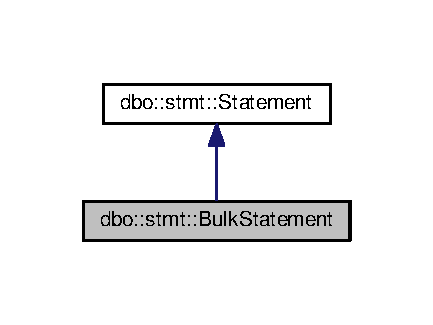
\includegraphics[width=208pt]{classdbo_1_1stmt_1_1_bulk_statement__inherit__graph}
\end{center}
\end{figure}


Collaboration diagram for dbo\+:\+:stmt\+:\+:Bulk\+Statement\+:\nopagebreak
\begin{figure}[H]
\begin{center}
\leavevmode
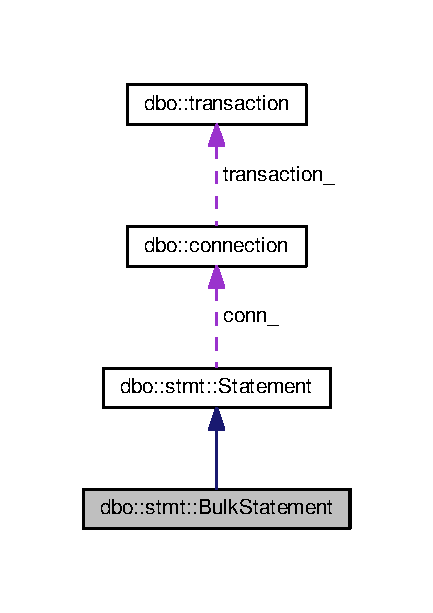
\includegraphics[width=208pt]{classdbo_1_1stmt_1_1_bulk_statement__coll__graph}
\end{center}
\end{figure}
\subsection*{Classes}
\begin{DoxyCompactItemize}
\item 
struct \hyperlink{structdbo_1_1stmt_1_1_bulk_statement_1_1_buffer}{Buffer}
\end{DoxyCompactItemize}
\subsection*{Public Member Functions}
\begin{DoxyCompactItemize}
\item 
\hyperlink{classdbo_1_1stmt_1_1_bulk_statement_a65ab5513c7c7ac521101f8373d160c8d}{Bulk\+Statement} (\hyperlink{classdbo_1_1connection}{connection} \&conn, const std\+::string \&table)
\item 
virtual \hyperlink{classdbo_1_1stmt_1_1_bulk_statement_ab6d5e3e1f6105d0a776c3a59a1e4ef1d}{$\sim$\+Bulk\+Statement} ()
\item 
virtual void \hyperlink{classdbo_1_1stmt_1_1_bulk_statement_ae40b794caf52eb3e1cafaef7eeb2042c}{bind} ()
\item 
virtual void \hyperlink{classdbo_1_1stmt_1_1_bulk_statement_ae12881728ef31a7acc0903d7473a8cb9}{bind} (const std\+::string \&value)
\item 
virtual void \hyperlink{classdbo_1_1stmt_1_1_bulk_statement_a36ca4fb16d32d17b838fe4604ebf2139}{bind} (const std\+::vector$<$ unsigned char $>$ \&value)
\item 
virtual bool \hyperlink{classdbo_1_1stmt_1_1_bulk_statement_ae789fa6e80389758303064fcceafb597}{read} (char $\ast$\&value)
\item 
virtual bool \hyperlink{classdbo_1_1stmt_1_1_bulk_statement_aaa5722c838af4203ae19bd94448d63dd}{read} (std\+::vector$<$ unsigned char $>$ \&value)
\item 
virtual void \hyperlink{classdbo_1_1stmt_1_1_bulk_statement_af2cde35cc87094525b4dc1e4dc99c710}{execute} ()
\item 
void \hyperlink{classdbo_1_1stmt_1_1_bulk_statement_ad9df1762cc49be8a6a377b69d3e3e3fd}{add\+Column} (const std\+::string \&name)
\item 
void \hyperlink{classdbo_1_1stmt_1_1_bulk_statement_a5ac1aa607b913ee63d3725f647169cbc}{prepare} ()
\item 
bool \hyperlink{classdbo_1_1stmt_1_1_bulk_statement_af80513fee94043fe22ac8797efd40139}{next\+Row} ()
\end{DoxyCompactItemize}
\subsection*{Protected Member Functions}
\begin{DoxyCompactItemize}
\item 
std\+::string \hyperlink{classdbo_1_1stmt_1_1_bulk_statement_a0ee84702a51bab063d0cceb089fb9f6a}{escape} (const std\+::string \&value)
\item 
std\+::string \hyperlink{classdbo_1_1stmt_1_1_bulk_statement_a6e6c2a2e00233b6bd5e994e9167f56be}{escape\+Hex} (const std\+::vector$<$ unsigned char $>$ \&value)
\item 
void \hyperlink{classdbo_1_1stmt_1_1_bulk_statement_a4e6304fec07499aff629472d6c834972}{add\+Data} (const char $\ast$data)
\item 
void \hyperlink{classdbo_1_1stmt_1_1_bulk_statement_af4bdeffa23bff4f22081b5f0b839f54b}{add\+Data} (const std\+::string \&data)
\end{DoxyCompactItemize}
\subsection*{Static Protected Member Functions}
\begin{DoxyCompactItemize}
\item 
static void \hyperlink{classdbo_1_1stmt_1_1_bulk_statement_ad68e1cff54f7121031985db6bab98362}{pg\+\_\+result\+\_\+deleter} (pg\+\_\+result $\ast$result)
\end{DoxyCompactItemize}
\subsection*{Protected Attributes}
\begin{DoxyCompactItemize}
\item 
size\+\_\+t \hyperlink{classdbo_1_1stmt_1_1_bulk_statement_a354e1122b8e8e2a43769e84f8858023d}{row\+\_\+}
\item 
size\+\_\+t \hyperlink{classdbo_1_1stmt_1_1_bulk_statement_aa4fe97f33a962eb6fd063537881a6607}{column\+\_\+}
\item 
std\+::string \hyperlink{classdbo_1_1stmt_1_1_bulk_statement_a15af921e3b69e401e9cb2416094dac46}{sep\+\_\+}
\item 
std\+::stringstream \hyperlink{classdbo_1_1stmt_1_1_bulk_statement_ac32b572232a8d0378d420cf44bbca623}{sql\+\_\+}
\item 
std\+::deque$<$ \hyperlink{structdbo_1_1stmt_1_1_bulk_statement_1_1_buffer}{Buffer} $>$ \hyperlink{classdbo_1_1stmt_1_1_bulk_statement_a13929be97455dc9cd060c50bcae537cf}{buffers\+\_\+}
\item 
std\+::string \hyperlink{classdbo_1_1stmt_1_1_bulk_statement_af3e99f5a3fe342a6295c96927c66c1ed}{table\+\_\+}
\item 
std\+::vector$<$ std\+::string $>$ \hyperlink{classdbo_1_1stmt_1_1_bulk_statement_a6879423d29e1b68dbe1039aad61a33bd}{columns\+\_\+}
\end{DoxyCompactItemize}
\subsection*{Static Protected Attributes}
\begin{DoxyCompactItemize}
\item 
static const size\+\_\+t \hyperlink{classdbo_1_1stmt_1_1_bulk_statement_a89930e2b8db959d397c099d37a4d7a59}{Buff\+Size} =sizeof(int)/2-\/1
\end{DoxyCompactItemize}


\subsection{Constructor \& Destructor Documentation}
\hypertarget{classdbo_1_1stmt_1_1_bulk_statement_a65ab5513c7c7ac521101f8373d160c8d}{\index{dbo\+::stmt\+::\+Bulk\+Statement@{dbo\+::stmt\+::\+Bulk\+Statement}!Bulk\+Statement@{Bulk\+Statement}}
\index{Bulk\+Statement@{Bulk\+Statement}!dbo\+::stmt\+::\+Bulk\+Statement@{dbo\+::stmt\+::\+Bulk\+Statement}}
\subsubsection[{Bulk\+Statement}]{\setlength{\rightskip}{0pt plus 5cm}Bulk\+Statement\+::\+Bulk\+Statement (
\begin{DoxyParamCaption}
\item[{{\bf connection} \&}]{conn, }
\item[{const std\+::string \&}]{table}
\end{DoxyParamCaption}
)}}\label{classdbo_1_1stmt_1_1_bulk_statement_a65ab5513c7c7ac521101f8373d160c8d}
Build a statement, the name of the statement will be created from the hash of the sql query \hypertarget{classdbo_1_1stmt_1_1_bulk_statement_ab6d5e3e1f6105d0a776c3a59a1e4ef1d}{\index{dbo\+::stmt\+::\+Bulk\+Statement@{dbo\+::stmt\+::\+Bulk\+Statement}!````~Bulk\+Statement@{$\sim$\+Bulk\+Statement}}
\index{````~Bulk\+Statement@{$\sim$\+Bulk\+Statement}!dbo\+::stmt\+::\+Bulk\+Statement@{dbo\+::stmt\+::\+Bulk\+Statement}}
\subsubsection[{$\sim$\+Bulk\+Statement}]{\setlength{\rightskip}{0pt plus 5cm}Bulk\+Statement\+::$\sim$\+Bulk\+Statement (
\begin{DoxyParamCaption}
{}
\end{DoxyParamCaption}
)\hspace{0.3cm}{\ttfamily [virtual]}}}\label{classdbo_1_1stmt_1_1_bulk_statement_ab6d5e3e1f6105d0a776c3a59a1e4ef1d}


\subsection{Member Function Documentation}
\hypertarget{classdbo_1_1stmt_1_1_bulk_statement_ad9df1762cc49be8a6a377b69d3e3e3fd}{\index{dbo\+::stmt\+::\+Bulk\+Statement@{dbo\+::stmt\+::\+Bulk\+Statement}!add\+Column@{add\+Column}}
\index{add\+Column@{add\+Column}!dbo\+::stmt\+::\+Bulk\+Statement@{dbo\+::stmt\+::\+Bulk\+Statement}}
\subsubsection[{add\+Column}]{\setlength{\rightskip}{0pt plus 5cm}void Bulk\+Statement\+::add\+Column (
\begin{DoxyParamCaption}
\item[{const std\+::string \&}]{name}
\end{DoxyParamCaption}
)}}\label{classdbo_1_1stmt_1_1_bulk_statement_ad9df1762cc49be8a6a377b69d3e3e3fd}
\hypertarget{classdbo_1_1stmt_1_1_bulk_statement_a4e6304fec07499aff629472d6c834972}{\index{dbo\+::stmt\+::\+Bulk\+Statement@{dbo\+::stmt\+::\+Bulk\+Statement}!add\+Data@{add\+Data}}
\index{add\+Data@{add\+Data}!dbo\+::stmt\+::\+Bulk\+Statement@{dbo\+::stmt\+::\+Bulk\+Statement}}
\subsubsection[{add\+Data}]{\setlength{\rightskip}{0pt plus 5cm}void Bulk\+Statement\+::add\+Data (
\begin{DoxyParamCaption}
\item[{const char $\ast$}]{data}
\end{DoxyParamCaption}
)\hspace{0.3cm}{\ttfamily [protected]}}}\label{classdbo_1_1stmt_1_1_bulk_statement_a4e6304fec07499aff629472d6c834972}
\hypertarget{classdbo_1_1stmt_1_1_bulk_statement_af4bdeffa23bff4f22081b5f0b839f54b}{\index{dbo\+::stmt\+::\+Bulk\+Statement@{dbo\+::stmt\+::\+Bulk\+Statement}!add\+Data@{add\+Data}}
\index{add\+Data@{add\+Data}!dbo\+::stmt\+::\+Bulk\+Statement@{dbo\+::stmt\+::\+Bulk\+Statement}}
\subsubsection[{add\+Data}]{\setlength{\rightskip}{0pt plus 5cm}void Bulk\+Statement\+::add\+Data (
\begin{DoxyParamCaption}
\item[{const std\+::string \&}]{data}
\end{DoxyParamCaption}
)\hspace{0.3cm}{\ttfamily [protected]}}}\label{classdbo_1_1stmt_1_1_bulk_statement_af4bdeffa23bff4f22081b5f0b839f54b}
\hypertarget{classdbo_1_1stmt_1_1_bulk_statement_ae40b794caf52eb3e1cafaef7eeb2042c}{\index{dbo\+::stmt\+::\+Bulk\+Statement@{dbo\+::stmt\+::\+Bulk\+Statement}!bind@{bind}}
\index{bind@{bind}!dbo\+::stmt\+::\+Bulk\+Statement@{dbo\+::stmt\+::\+Bulk\+Statement}}
\subsubsection[{bind}]{\setlength{\rightskip}{0pt plus 5cm}void Bulk\+Statement\+::bind (
\begin{DoxyParamCaption}
{}
\end{DoxyParamCaption}
)\hspace{0.3cm}{\ttfamily [virtual]}}}\label{classdbo_1_1stmt_1_1_bulk_statement_ae40b794caf52eb3e1cafaef7eeb2042c}
Bind a null value 

Implements \hyperlink{classdbo_1_1stmt_1_1_statement_a1699d7873785908a99211c91350cd376}{dbo\+::stmt\+::\+Statement}.

\hypertarget{classdbo_1_1stmt_1_1_bulk_statement_ae12881728ef31a7acc0903d7473a8cb9}{\index{dbo\+::stmt\+::\+Bulk\+Statement@{dbo\+::stmt\+::\+Bulk\+Statement}!bind@{bind}}
\index{bind@{bind}!dbo\+::stmt\+::\+Bulk\+Statement@{dbo\+::stmt\+::\+Bulk\+Statement}}
\subsubsection[{bind}]{\setlength{\rightskip}{0pt plus 5cm}void Bulk\+Statement\+::bind (
\begin{DoxyParamCaption}
\item[{const std\+::string \&}]{value}
\end{DoxyParamCaption}
)\hspace{0.3cm}{\ttfamily [virtual]}}}\label{classdbo_1_1stmt_1_1_bulk_statement_ae12881728ef31a7acc0903d7473a8cb9}
Bind a string value 

Implements \hyperlink{classdbo_1_1stmt_1_1_statement_a8f2897467f5fccaec72ffe5ad797a8a3}{dbo\+::stmt\+::\+Statement}.

\hypertarget{classdbo_1_1stmt_1_1_bulk_statement_a36ca4fb16d32d17b838fe4604ebf2139}{\index{dbo\+::stmt\+::\+Bulk\+Statement@{dbo\+::stmt\+::\+Bulk\+Statement}!bind@{bind}}
\index{bind@{bind}!dbo\+::stmt\+::\+Bulk\+Statement@{dbo\+::stmt\+::\+Bulk\+Statement}}
\subsubsection[{bind}]{\setlength{\rightskip}{0pt plus 5cm}void Bulk\+Statement\+::bind (
\begin{DoxyParamCaption}
\item[{const std\+::vector$<$ unsigned char $>$ \&}]{value}
\end{DoxyParamCaption}
)\hspace{0.3cm}{\ttfamily [virtual]}}}\label{classdbo_1_1stmt_1_1_bulk_statement_a36ca4fb16d32d17b838fe4604ebf2139}
Bind a binary value 

Implements \hyperlink{classdbo_1_1stmt_1_1_statement_a3f4f506b3df6f2d8667fa2900a662ee4}{dbo\+::stmt\+::\+Statement}.

\hypertarget{classdbo_1_1stmt_1_1_bulk_statement_a0ee84702a51bab063d0cceb089fb9f6a}{\index{dbo\+::stmt\+::\+Bulk\+Statement@{dbo\+::stmt\+::\+Bulk\+Statement}!escape@{escape}}
\index{escape@{escape}!dbo\+::stmt\+::\+Bulk\+Statement@{dbo\+::stmt\+::\+Bulk\+Statement}}
\subsubsection[{escape}]{\setlength{\rightskip}{0pt plus 5cm}std\+::string Bulk\+Statement\+::escape (
\begin{DoxyParamCaption}
\item[{const std\+::string \&}]{value}
\end{DoxyParamCaption}
)\hspace{0.3cm}{\ttfamily [protected]}}}\label{classdbo_1_1stmt_1_1_bulk_statement_a0ee84702a51bab063d0cceb089fb9f6a}
\hypertarget{classdbo_1_1stmt_1_1_bulk_statement_a6e6c2a2e00233b6bd5e994e9167f56be}{\index{dbo\+::stmt\+::\+Bulk\+Statement@{dbo\+::stmt\+::\+Bulk\+Statement}!escape\+Hex@{escape\+Hex}}
\index{escape\+Hex@{escape\+Hex}!dbo\+::stmt\+::\+Bulk\+Statement@{dbo\+::stmt\+::\+Bulk\+Statement}}
\subsubsection[{escape\+Hex}]{\setlength{\rightskip}{0pt plus 5cm}std\+::string Bulk\+Statement\+::escape\+Hex (
\begin{DoxyParamCaption}
\item[{const std\+::vector$<$ unsigned char $>$ \&}]{value}
\end{DoxyParamCaption}
)\hspace{0.3cm}{\ttfamily [protected]}}}\label{classdbo_1_1stmt_1_1_bulk_statement_a6e6c2a2e00233b6bd5e994e9167f56be}
\hypertarget{classdbo_1_1stmt_1_1_bulk_statement_af2cde35cc87094525b4dc1e4dc99c710}{\index{dbo\+::stmt\+::\+Bulk\+Statement@{dbo\+::stmt\+::\+Bulk\+Statement}!execute@{execute}}
\index{execute@{execute}!dbo\+::stmt\+::\+Bulk\+Statement@{dbo\+::stmt\+::\+Bulk\+Statement}}
\subsubsection[{execute}]{\setlength{\rightskip}{0pt plus 5cm}void Bulk\+Statement\+::execute (
\begin{DoxyParamCaption}
{}
\end{DoxyParamCaption}
)\hspace{0.3cm}{\ttfamily [virtual]}}}\label{classdbo_1_1stmt_1_1_bulk_statement_af2cde35cc87094525b4dc1e4dc99c710}
Execute the prepared statement 

Implements \hyperlink{classdbo_1_1stmt_1_1_statement_af8e1a95b6c0c8b8ac6f5a25f4c48bf5e}{dbo\+::stmt\+::\+Statement}.

\hypertarget{classdbo_1_1stmt_1_1_bulk_statement_af80513fee94043fe22ac8797efd40139}{\index{dbo\+::stmt\+::\+Bulk\+Statement@{dbo\+::stmt\+::\+Bulk\+Statement}!next\+Row@{next\+Row}}
\index{next\+Row@{next\+Row}!dbo\+::stmt\+::\+Bulk\+Statement@{dbo\+::stmt\+::\+Bulk\+Statement}}
\subsubsection[{next\+Row}]{\setlength{\rightskip}{0pt plus 5cm}bool Bulk\+Statement\+::next\+Row (
\begin{DoxyParamCaption}
{}
\end{DoxyParamCaption}
)}}\label{classdbo_1_1stmt_1_1_bulk_statement_af80513fee94043fe22ac8797efd40139}
\hypertarget{classdbo_1_1stmt_1_1_bulk_statement_ad68e1cff54f7121031985db6bab98362}{\index{dbo\+::stmt\+::\+Bulk\+Statement@{dbo\+::stmt\+::\+Bulk\+Statement}!pg\+\_\+result\+\_\+deleter@{pg\+\_\+result\+\_\+deleter}}
\index{pg\+\_\+result\+\_\+deleter@{pg\+\_\+result\+\_\+deleter}!dbo\+::stmt\+::\+Bulk\+Statement@{dbo\+::stmt\+::\+Bulk\+Statement}}
\subsubsection[{pg\+\_\+result\+\_\+deleter}]{\setlength{\rightskip}{0pt plus 5cm}void Bulk\+Statement\+::pg\+\_\+result\+\_\+deleter (
\begin{DoxyParamCaption}
\item[{pg\+\_\+result $\ast$}]{result}
\end{DoxyParamCaption}
)\hspace{0.3cm}{\ttfamily [static]}, {\ttfamily [protected]}}}\label{classdbo_1_1stmt_1_1_bulk_statement_ad68e1cff54f7121031985db6bab98362}
\hypertarget{classdbo_1_1stmt_1_1_bulk_statement_a5ac1aa607b913ee63d3725f647169cbc}{\index{dbo\+::stmt\+::\+Bulk\+Statement@{dbo\+::stmt\+::\+Bulk\+Statement}!prepare@{prepare}}
\index{prepare@{prepare}!dbo\+::stmt\+::\+Bulk\+Statement@{dbo\+::stmt\+::\+Bulk\+Statement}}
\subsubsection[{prepare}]{\setlength{\rightskip}{0pt plus 5cm}void Bulk\+Statement\+::prepare (
\begin{DoxyParamCaption}
{}
\end{DoxyParamCaption}
)}}\label{classdbo_1_1stmt_1_1_bulk_statement_a5ac1aa607b913ee63d3725f647169cbc}
\hypertarget{classdbo_1_1stmt_1_1_bulk_statement_ae789fa6e80389758303064fcceafb597}{\index{dbo\+::stmt\+::\+Bulk\+Statement@{dbo\+::stmt\+::\+Bulk\+Statement}!read@{read}}
\index{read@{read}!dbo\+::stmt\+::\+Bulk\+Statement@{dbo\+::stmt\+::\+Bulk\+Statement}}
\subsubsection[{read}]{\setlength{\rightskip}{0pt plus 5cm}bool Bulk\+Statement\+::read (
\begin{DoxyParamCaption}
\item[{char $\ast$\&}]{value}
\end{DoxyParamCaption}
)\hspace{0.3cm}{\ttfamily [virtual]}}}\label{classdbo_1_1stmt_1_1_bulk_statement_ae789fa6e80389758303064fcceafb597}
Read content to string 

Implements \hyperlink{classdbo_1_1stmt_1_1_statement_a98ea71bb3c771dc5831b39d74035eb6b}{dbo\+::stmt\+::\+Statement}.

\hypertarget{classdbo_1_1stmt_1_1_bulk_statement_aaa5722c838af4203ae19bd94448d63dd}{\index{dbo\+::stmt\+::\+Bulk\+Statement@{dbo\+::stmt\+::\+Bulk\+Statement}!read@{read}}
\index{read@{read}!dbo\+::stmt\+::\+Bulk\+Statement@{dbo\+::stmt\+::\+Bulk\+Statement}}
\subsubsection[{read}]{\setlength{\rightskip}{0pt plus 5cm}bool Bulk\+Statement\+::read (
\begin{DoxyParamCaption}
\item[{std\+::vector$<$ unsigned char $>$ \&}]{value}
\end{DoxyParamCaption}
)\hspace{0.3cm}{\ttfamily [virtual]}}}\label{classdbo_1_1stmt_1_1_bulk_statement_aaa5722c838af4203ae19bd94448d63dd}
Read content to binary array 

Implements \hyperlink{classdbo_1_1stmt_1_1_statement_a45864352cde548530425119915b3a2ef}{dbo\+::stmt\+::\+Statement}.



\subsection{Member Data Documentation}
\hypertarget{classdbo_1_1stmt_1_1_bulk_statement_a13929be97455dc9cd060c50bcae537cf}{\index{dbo\+::stmt\+::\+Bulk\+Statement@{dbo\+::stmt\+::\+Bulk\+Statement}!buffers\+\_\+@{buffers\+\_\+}}
\index{buffers\+\_\+@{buffers\+\_\+}!dbo\+::stmt\+::\+Bulk\+Statement@{dbo\+::stmt\+::\+Bulk\+Statement}}
\subsubsection[{buffers\+\_\+}]{\setlength{\rightskip}{0pt plus 5cm}std\+::deque$<${\bf Buffer}$>$ dbo\+::stmt\+::\+Bulk\+Statement\+::buffers\+\_\+\hspace{0.3cm}{\ttfamily [protected]}}}\label{classdbo_1_1stmt_1_1_bulk_statement_a13929be97455dc9cd060c50bcae537cf}
\hypertarget{classdbo_1_1stmt_1_1_bulk_statement_a89930e2b8db959d397c099d37a4d7a59}{\index{dbo\+::stmt\+::\+Bulk\+Statement@{dbo\+::stmt\+::\+Bulk\+Statement}!Buff\+Size@{Buff\+Size}}
\index{Buff\+Size@{Buff\+Size}!dbo\+::stmt\+::\+Bulk\+Statement@{dbo\+::stmt\+::\+Bulk\+Statement}}
\subsubsection[{Buff\+Size}]{\setlength{\rightskip}{0pt plus 5cm}const size\+\_\+t dbo\+::stmt\+::\+Bulk\+Statement\+::\+Buff\+Size =sizeof(int)/2-\/1\hspace{0.3cm}{\ttfamily [static]}, {\ttfamily [protected]}}}\label{classdbo_1_1stmt_1_1_bulk_statement_a89930e2b8db959d397c099d37a4d7a59}
\hypertarget{classdbo_1_1stmt_1_1_bulk_statement_aa4fe97f33a962eb6fd063537881a6607}{\index{dbo\+::stmt\+::\+Bulk\+Statement@{dbo\+::stmt\+::\+Bulk\+Statement}!column\+\_\+@{column\+\_\+}}
\index{column\+\_\+@{column\+\_\+}!dbo\+::stmt\+::\+Bulk\+Statement@{dbo\+::stmt\+::\+Bulk\+Statement}}
\subsubsection[{column\+\_\+}]{\setlength{\rightskip}{0pt plus 5cm}size\+\_\+t dbo\+::stmt\+::\+Bulk\+Statement\+::column\+\_\+\hspace{0.3cm}{\ttfamily [protected]}}}\label{classdbo_1_1stmt_1_1_bulk_statement_aa4fe97f33a962eb6fd063537881a6607}
\hypertarget{classdbo_1_1stmt_1_1_bulk_statement_a6879423d29e1b68dbe1039aad61a33bd}{\index{dbo\+::stmt\+::\+Bulk\+Statement@{dbo\+::stmt\+::\+Bulk\+Statement}!columns\+\_\+@{columns\+\_\+}}
\index{columns\+\_\+@{columns\+\_\+}!dbo\+::stmt\+::\+Bulk\+Statement@{dbo\+::stmt\+::\+Bulk\+Statement}}
\subsubsection[{columns\+\_\+}]{\setlength{\rightskip}{0pt plus 5cm}std\+::vector$<$std\+::string$>$ dbo\+::stmt\+::\+Bulk\+Statement\+::columns\+\_\+\hspace{0.3cm}{\ttfamily [protected]}}}\label{classdbo_1_1stmt_1_1_bulk_statement_a6879423d29e1b68dbe1039aad61a33bd}
\hypertarget{classdbo_1_1stmt_1_1_bulk_statement_a354e1122b8e8e2a43769e84f8858023d}{\index{dbo\+::stmt\+::\+Bulk\+Statement@{dbo\+::stmt\+::\+Bulk\+Statement}!row\+\_\+@{row\+\_\+}}
\index{row\+\_\+@{row\+\_\+}!dbo\+::stmt\+::\+Bulk\+Statement@{dbo\+::stmt\+::\+Bulk\+Statement}}
\subsubsection[{row\+\_\+}]{\setlength{\rightskip}{0pt plus 5cm}size\+\_\+t dbo\+::stmt\+::\+Bulk\+Statement\+::row\+\_\+\hspace{0.3cm}{\ttfamily [protected]}}}\label{classdbo_1_1stmt_1_1_bulk_statement_a354e1122b8e8e2a43769e84f8858023d}
\hypertarget{classdbo_1_1stmt_1_1_bulk_statement_a15af921e3b69e401e9cb2416094dac46}{\index{dbo\+::stmt\+::\+Bulk\+Statement@{dbo\+::stmt\+::\+Bulk\+Statement}!sep\+\_\+@{sep\+\_\+}}
\index{sep\+\_\+@{sep\+\_\+}!dbo\+::stmt\+::\+Bulk\+Statement@{dbo\+::stmt\+::\+Bulk\+Statement}}
\subsubsection[{sep\+\_\+}]{\setlength{\rightskip}{0pt plus 5cm}std\+::string dbo\+::stmt\+::\+Bulk\+Statement\+::sep\+\_\+\hspace{0.3cm}{\ttfamily [protected]}}}\label{classdbo_1_1stmt_1_1_bulk_statement_a15af921e3b69e401e9cb2416094dac46}
\hypertarget{classdbo_1_1stmt_1_1_bulk_statement_ac32b572232a8d0378d420cf44bbca623}{\index{dbo\+::stmt\+::\+Bulk\+Statement@{dbo\+::stmt\+::\+Bulk\+Statement}!sql\+\_\+@{sql\+\_\+}}
\index{sql\+\_\+@{sql\+\_\+}!dbo\+::stmt\+::\+Bulk\+Statement@{dbo\+::stmt\+::\+Bulk\+Statement}}
\subsubsection[{sql\+\_\+}]{\setlength{\rightskip}{0pt plus 5cm}std\+::stringstream dbo\+::stmt\+::\+Bulk\+Statement\+::sql\+\_\+\hspace{0.3cm}{\ttfamily [protected]}}}\label{classdbo_1_1stmt_1_1_bulk_statement_ac32b572232a8d0378d420cf44bbca623}
\hypertarget{classdbo_1_1stmt_1_1_bulk_statement_af3e99f5a3fe342a6295c96927c66c1ed}{\index{dbo\+::stmt\+::\+Bulk\+Statement@{dbo\+::stmt\+::\+Bulk\+Statement}!table\+\_\+@{table\+\_\+}}
\index{table\+\_\+@{table\+\_\+}!dbo\+::stmt\+::\+Bulk\+Statement@{dbo\+::stmt\+::\+Bulk\+Statement}}
\subsubsection[{table\+\_\+}]{\setlength{\rightskip}{0pt plus 5cm}std\+::string dbo\+::stmt\+::\+Bulk\+Statement\+::table\+\_\+\hspace{0.3cm}{\ttfamily [protected]}}}\label{classdbo_1_1stmt_1_1_bulk_statement_af3e99f5a3fe342a6295c96927c66c1ed}


The documentation for this class was generated from the following files\+:\begin{DoxyCompactItemize}
\item 
dbo/stmt/\hyperlink{_bulk_statement_8h}{Bulk\+Statement.\+h}\item 
dbo/stmt/\hyperlink{_bulk_statement_8cpp}{Bulk\+Statement.\+cpp}\end{DoxyCompactItemize}

\hypertarget{classdbo_1_1collection}{\section{dbo\+:\+:collection$<$ C $>$ Class Template Reference}
\label{classdbo_1_1collection}\index{dbo\+::collection$<$ C $>$@{dbo\+::collection$<$ C $>$}}
}


{\ttfamily \#include $<$collection.\+hpp$>$}

\subsection*{Classes}
\begin{DoxyCompactItemize}
\item 
class \hyperlink{classdbo_1_1collection_1_1iterator}{iterator}
\end{DoxyCompactItemize}
\subsection*{Public Types}
\begin{DoxyCompactItemize}
\item 
using \hyperlink{classdbo_1_1collection_ad004dc216c503f08d75c1d3e3fffe803}{Id\+Type} = typename \hyperlink{structdbo_1_1traits_1_1dbo__traits}{traits\+::dbo\+\_\+traits}$<$ C $>$\+::\hyperlink{classdbo_1_1collection_ad004dc216c503f08d75c1d3e3fffe803}{Id\+Type}
\end{DoxyCompactItemize}
\subsection*{Public Member Functions}
\begin{DoxyCompactItemize}
\item 
\hyperlink{classdbo_1_1collection_ae50f29fec46adcb871f7aad48dcfea15}{collection} ()
\begin{DoxyCompactList}\small\item\em Default constructor. \end{DoxyCompactList}\item 
\hyperlink{classdbo_1_1collection_a3f4798e657f21b7dabf5f2ad8c408a03}{collection} (const \hyperlink{classdbo_1_1collection}{collection}$<$ C $>$ \&other)
\begin{DoxyCompactList}\small\item\em Copy constructor. \end{DoxyCompactList}\item 
\hyperlink{classdbo_1_1collection_a4cc94ece60b1a87f99c250ef55eef3e4}{$\sim$collection} ()
\begin{DoxyCompactList}\small\item\em Destructor. \end{DoxyCompactList}\item 
\hyperlink{classdbo_1_1collection}{collection}$<$ C $>$ \& \hyperlink{classdbo_1_1collection_a0c43d0bf6e86d59bd0e10f8100e76ee7}{operator=} (const \hyperlink{classdbo_1_1collection}{collection}$<$ C $>$ \&other)
\begin{DoxyCompactList}\small\item\em Assignment operator. \end{DoxyCompactList}\item 
void \hyperlink{classdbo_1_1collection_a207e270b7df92cea700a640a5ac359e5}{push\+\_\+back} (const \hyperlink{classdbo_1_1ptr}{ptr}$<$ C $>$ \&\hyperlink{classdbo_1_1ptr}{ptr})
\item 
void \hyperlink{classdbo_1_1collection_a48e3718fafd427fcf05f6508b3ffe818}{clear} ()
\item 
\hyperlink{classdbo_1_1collection_1_1iterator}{iterator} \hyperlink{classdbo_1_1collection_a963843d0db110b4eeeb5851d957cd545}{begin} ()
\begin{DoxyCompactList}\small\item\em Returns an iterator to the begin of the collection. \end{DoxyCompactList}\item 
\hyperlink{classdbo_1_1collection_1_1iterator}{iterator} \hyperlink{classdbo_1_1collection_a9a0ffa8e99ded7d024a0847597e32f21}{end} ()
\begin{DoxyCompactList}\small\item\em Returns an iterator to the end of the collection. \end{DoxyCompactList}\item 
size\+\_\+t \hyperlink{classdbo_1_1collection_ad0f7875f9a095559335d20583c655a30}{size} ()
\item 
bool \hyperlink{classdbo_1_1collection_aec3e88df5f1f281d7f0366a86e6d9565}{empty} ()
\end{DoxyCompactItemize}
\subsection*{Protected Types}
\begin{DoxyCompactItemize}
\item 
using \hyperlink{classdbo_1_1collection_a5d509fade7beb175d427ffca3dc9559f}{Ptr} = typename \hyperlink{classdbo_1_1ptr}{ptr}$<$ C $>$\+::\hyperlink{classdbo_1_1collection_a5d509fade7beb175d427ffca3dc9559f}{Ptr}
\end{DoxyCompactItemize}
\subsection*{Protected Member Functions}
\begin{DoxyCompactItemize}
\item 
void \hyperlink{classdbo_1_1collection_ab6fd1148b56a8370eb9a354f0c19f99f}{free} (\hyperlink{classdbo_1_1collection_a5d509fade7beb175d427ffca3dc9559f}{Ptr} $\ast$\&\hyperlink{classdbo_1_1ptr}{ptr})
\item 
void \hyperlink{classdbo_1_1collection_a5d1235d48ba1a6c0abb28a86050cce78}{take} (\hyperlink{classdbo_1_1collection_a5d509fade7beb175d427ffca3dc9559f}{Ptr} $\ast$\&\hyperlink{classdbo_1_1ptr}{ptr})
\end{DoxyCompactItemize}
\subsection*{Protected Attributes}
\begin{DoxyCompactItemize}
\item 
std\+::deque$<$ \hyperlink{classdbo_1_1collection_a5d509fade7beb175d427ffca3dc9559f}{Ptr} $\ast$ $>$ \hyperlink{classdbo_1_1collection_a868d7d3bfb98c3a4f739e48043aeaba3}{ptrs\+\_\+}
\item 
char $\ast$ \hyperlink{classdbo_1_1collection_a8b18a6670d28cfc6e6ace16ce62c2609}{table\+Name\+\_\+}
\end{DoxyCompactItemize}
\subsection*{Static Protected Attributes}
\begin{DoxyCompactItemize}
\item 
static \hyperlink{classdbo_1_1collection_ad004dc216c503f08d75c1d3e3fffe803}{Id\+Type} \hyperlink{classdbo_1_1collection_af3537bd847de5995e84cf83649276001}{invalid\+Id\+\_\+} =\hyperlink{structdbo_1_1traits_1_1dbo__traits}{traits\+::dbo\+\_\+traits}$<$C$>$\+::invalid\+Id()
\end{DoxyCompactItemize}


\subsection{Member Typedef Documentation}
\hypertarget{classdbo_1_1collection_ad004dc216c503f08d75c1d3e3fffe803}{\index{dbo\+::collection@{dbo\+::collection}!Id\+Type@{Id\+Type}}
\index{Id\+Type@{Id\+Type}!dbo\+::collection@{dbo\+::collection}}
\subsubsection[{Id\+Type}]{\setlength{\rightskip}{0pt plus 5cm}template$<$class C$>$ using {\bf dbo\+::collection}$<$ C $>$\+::{\bf Id\+Type} =  typename {\bf traits\+::dbo\+\_\+traits}$<$C$>$\+::{\bf Id\+Type}}}\label{classdbo_1_1collection_ad004dc216c503f08d75c1d3e3fffe803}
\hypertarget{classdbo_1_1collection_a5d509fade7beb175d427ffca3dc9559f}{\index{dbo\+::collection@{dbo\+::collection}!Ptr@{Ptr}}
\index{Ptr@{Ptr}!dbo\+::collection@{dbo\+::collection}}
\subsubsection[{Ptr}]{\setlength{\rightskip}{0pt plus 5cm}template$<$class C$>$ using {\bf dbo\+::collection}$<$ C $>$\+::{\bf Ptr} =  typename {\bf ptr}$<$C$>$\+::{\bf Ptr}\hspace{0.3cm}{\ttfamily [protected]}}}\label{classdbo_1_1collection_a5d509fade7beb175d427ffca3dc9559f}


\subsection{Constructor \& Destructor Documentation}
\hypertarget{classdbo_1_1collection_ae50f29fec46adcb871f7aad48dcfea15}{\index{dbo\+::collection@{dbo\+::collection}!collection@{collection}}
\index{collection@{collection}!dbo\+::collection@{dbo\+::collection}}
\subsubsection[{collection}]{\setlength{\rightskip}{0pt plus 5cm}template$<$class C $>$ {\bf dbo\+::collection}$<$ C $>$\+::{\bf collection} (
\begin{DoxyParamCaption}
{}
\end{DoxyParamCaption}
)}}\label{classdbo_1_1collection_ae50f29fec46adcb871f7aad48dcfea15}


Default constructor. 

Constructs an empty collection that is not bound to a table or query \hypertarget{classdbo_1_1collection_a3f4798e657f21b7dabf5f2ad8c408a03}{\index{dbo\+::collection@{dbo\+::collection}!collection@{collection}}
\index{collection@{collection}!dbo\+::collection@{dbo\+::collection}}
\subsubsection[{collection}]{\setlength{\rightskip}{0pt plus 5cm}template$<$class C $>$ {\bf dbo\+::collection}$<$ C $>$\+::{\bf collection} (
\begin{DoxyParamCaption}
\item[{const {\bf collection}$<$ C $>$ \&}]{other}
\end{DoxyParamCaption}
)}}\label{classdbo_1_1collection_a3f4798e657f21b7dabf5f2ad8c408a03}


Copy constructor. 

\hypertarget{classdbo_1_1collection_a4cc94ece60b1a87f99c250ef55eef3e4}{\index{dbo\+::collection@{dbo\+::collection}!````~collection@{$\sim$collection}}
\index{````~collection@{$\sim$collection}!dbo\+::collection@{dbo\+::collection}}
\subsubsection[{$\sim$collection}]{\setlength{\rightskip}{0pt plus 5cm}template$<$class C $>$ {\bf dbo\+::collection}$<$ C $>$\+::$\sim${\bf collection} (
\begin{DoxyParamCaption}
{}
\end{DoxyParamCaption}
)}}\label{classdbo_1_1collection_a4cc94ece60b1a87f99c250ef55eef3e4}


Destructor. 



\subsection{Member Function Documentation}
\hypertarget{classdbo_1_1collection_a963843d0db110b4eeeb5851d957cd545}{\index{dbo\+::collection@{dbo\+::collection}!begin@{begin}}
\index{begin@{begin}!dbo\+::collection@{dbo\+::collection}}
\subsubsection[{begin}]{\setlength{\rightskip}{0pt plus 5cm}template$<$class C $>$ {\bf collection}$<$ C $>$\+::{\bf iterator} {\bf dbo\+::collection}$<$ C $>$\+::begin (
\begin{DoxyParamCaption}
{}
\end{DoxyParamCaption}
)}}\label{classdbo_1_1collection_a963843d0db110b4eeeb5851d957cd545}


Returns an iterator to the begin of the collection. 

\begin{DoxySeeAlso}{See also}
\hyperlink{classdbo_1_1collection_a9a0ffa8e99ded7d024a0847597e32f21}{end()} 
\end{DoxySeeAlso}
\hypertarget{classdbo_1_1collection_a48e3718fafd427fcf05f6508b3ffe818}{\index{dbo\+::collection@{dbo\+::collection}!clear@{clear}}
\index{clear@{clear}!dbo\+::collection@{dbo\+::collection}}
\subsubsection[{clear}]{\setlength{\rightskip}{0pt plus 5cm}template$<$class C $>$ void {\bf dbo\+::collection}$<$ C $>$\+::clear (
\begin{DoxyParamCaption}
{}
\end{DoxyParamCaption}
)}}\label{classdbo_1_1collection_a48e3718fafd427fcf05f6508b3ffe818}
\hypertarget{classdbo_1_1collection_aec3e88df5f1f281d7f0366a86e6d9565}{\index{dbo\+::collection@{dbo\+::collection}!empty@{empty}}
\index{empty@{empty}!dbo\+::collection@{dbo\+::collection}}
\subsubsection[{empty}]{\setlength{\rightskip}{0pt plus 5cm}template$<$class C $>$ bool {\bf dbo\+::collection}$<$ C $>$\+::empty (
\begin{DoxyParamCaption}
{}
\end{DoxyParamCaption}
)}}\label{classdbo_1_1collection_aec3e88df5f1f281d7f0366a86e6d9565}
\hypertarget{classdbo_1_1collection_a9a0ffa8e99ded7d024a0847597e32f21}{\index{dbo\+::collection@{dbo\+::collection}!end@{end}}
\index{end@{end}!dbo\+::collection@{dbo\+::collection}}
\subsubsection[{end}]{\setlength{\rightskip}{0pt plus 5cm}template$<$class C $>$ {\bf collection}$<$ C $>$\+::{\bf iterator} {\bf dbo\+::collection}$<$ C $>$\+::end (
\begin{DoxyParamCaption}
{}
\end{DoxyParamCaption}
)}}\label{classdbo_1_1collection_a9a0ffa8e99ded7d024a0847597e32f21}


Returns an iterator to the end of the collection. 

\begin{DoxySeeAlso}{See also}
\hyperlink{classdbo_1_1collection_a963843d0db110b4eeeb5851d957cd545}{begin()} 
\end{DoxySeeAlso}
\hypertarget{classdbo_1_1collection_ab6fd1148b56a8370eb9a354f0c19f99f}{\index{dbo\+::collection@{dbo\+::collection}!free@{free}}
\index{free@{free}!dbo\+::collection@{dbo\+::collection}}
\subsubsection[{free}]{\setlength{\rightskip}{0pt plus 5cm}template$<$class C $>$ void {\bf dbo\+::collection}$<$ C $>$\+::free (
\begin{DoxyParamCaption}
\item[{{\bf Ptr} $\ast$\&}]{ptr}
\end{DoxyParamCaption}
)\hspace{0.3cm}{\ttfamily [protected]}}}\label{classdbo_1_1collection_ab6fd1148b56a8370eb9a354f0c19f99f}
\hypertarget{classdbo_1_1collection_a0c43d0bf6e86d59bd0e10f8100e76ee7}{\index{dbo\+::collection@{dbo\+::collection}!operator=@{operator=}}
\index{operator=@{operator=}!dbo\+::collection@{dbo\+::collection}}
\subsubsection[{operator=}]{\setlength{\rightskip}{0pt plus 5cm}template$<$class C $>$ {\bf collection}$<$ C $>$ \& {\bf dbo\+::collection}$<$ C $>$\+::operator= (
\begin{DoxyParamCaption}
\item[{const {\bf collection}$<$ C $>$ \&}]{other}
\end{DoxyParamCaption}
)}}\label{classdbo_1_1collection_a0c43d0bf6e86d59bd0e10f8100e76ee7}


Assignment operator. 

\hypertarget{classdbo_1_1collection_a207e270b7df92cea700a640a5ac359e5}{\index{dbo\+::collection@{dbo\+::collection}!push\+\_\+back@{push\+\_\+back}}
\index{push\+\_\+back@{push\+\_\+back}!dbo\+::collection@{dbo\+::collection}}
\subsubsection[{push\+\_\+back}]{\setlength{\rightskip}{0pt plus 5cm}template$<$class C $>$ void {\bf dbo\+::collection}$<$ C $>$\+::push\+\_\+back (
\begin{DoxyParamCaption}
\item[{const {\bf ptr}$<$ C $>$ \&}]{ptr}
\end{DoxyParamCaption}
)}}\label{classdbo_1_1collection_a207e270b7df92cea700a640a5ac359e5}
\hypertarget{classdbo_1_1collection_ad0f7875f9a095559335d20583c655a30}{\index{dbo\+::collection@{dbo\+::collection}!size@{size}}
\index{size@{size}!dbo\+::collection@{dbo\+::collection}}
\subsubsection[{size}]{\setlength{\rightskip}{0pt plus 5cm}template$<$class C $>$ size\+\_\+t {\bf dbo\+::collection}$<$ C $>$\+::size (
\begin{DoxyParamCaption}
{}
\end{DoxyParamCaption}
)}}\label{classdbo_1_1collection_ad0f7875f9a095559335d20583c655a30}
\hypertarget{classdbo_1_1collection_a5d1235d48ba1a6c0abb28a86050cce78}{\index{dbo\+::collection@{dbo\+::collection}!take@{take}}
\index{take@{take}!dbo\+::collection@{dbo\+::collection}}
\subsubsection[{take}]{\setlength{\rightskip}{0pt plus 5cm}template$<$class C $>$ void {\bf dbo\+::collection}$<$ C $>$\+::take (
\begin{DoxyParamCaption}
\item[{{\bf Ptr} $\ast$\&}]{ptr}
\end{DoxyParamCaption}
)\hspace{0.3cm}{\ttfamily [protected]}}}\label{classdbo_1_1collection_a5d1235d48ba1a6c0abb28a86050cce78}


\subsection{Member Data Documentation}
\hypertarget{classdbo_1_1collection_af3537bd847de5995e84cf83649276001}{\index{dbo\+::collection@{dbo\+::collection}!invalid\+Id\+\_\+@{invalid\+Id\+\_\+}}
\index{invalid\+Id\+\_\+@{invalid\+Id\+\_\+}!dbo\+::collection@{dbo\+::collection}}
\subsubsection[{invalid\+Id\+\_\+}]{\setlength{\rightskip}{0pt plus 5cm}template$<$class C$>$ {\bf collection}$<$ C $>$\+::{\bf Id\+Type} {\bf dbo\+::collection}$<$ C $>$\+::invalid\+Id\+\_\+ ={\bf traits\+::dbo\+\_\+traits}$<$C$>$\+::invalid\+Id()\hspace{0.3cm}{\ttfamily [static]}, {\ttfamily [protected]}}}\label{classdbo_1_1collection_af3537bd847de5995e84cf83649276001}
\hypertarget{classdbo_1_1collection_a868d7d3bfb98c3a4f739e48043aeaba3}{\index{dbo\+::collection@{dbo\+::collection}!ptrs\+\_\+@{ptrs\+\_\+}}
\index{ptrs\+\_\+@{ptrs\+\_\+}!dbo\+::collection@{dbo\+::collection}}
\subsubsection[{ptrs\+\_\+}]{\setlength{\rightskip}{0pt plus 5cm}template$<$class C$>$ std\+::deque$<${\bf Ptr}$\ast$$>$ {\bf dbo\+::collection}$<$ C $>$\+::ptrs\+\_\+\hspace{0.3cm}{\ttfamily [protected]}}}\label{classdbo_1_1collection_a868d7d3bfb98c3a4f739e48043aeaba3}
\hypertarget{classdbo_1_1collection_a8b18a6670d28cfc6e6ace16ce62c2609}{\index{dbo\+::collection@{dbo\+::collection}!table\+Name\+\_\+@{table\+Name\+\_\+}}
\index{table\+Name\+\_\+@{table\+Name\+\_\+}!dbo\+::collection@{dbo\+::collection}}
\subsubsection[{table\+Name\+\_\+}]{\setlength{\rightskip}{0pt plus 5cm}template$<$class C$>$ char$\ast$ {\bf dbo\+::collection}$<$ C $>$\+::table\+Name\+\_\+\hspace{0.3cm}{\ttfamily [protected]}}}\label{classdbo_1_1collection_a8b18a6670d28cfc6e6ace16ce62c2609}


The documentation for this class was generated from the following files\+:\begin{DoxyCompactItemize}
\item 
dbo/\hyperlink{collection_8hpp}{collection.\+hpp}\item 
dbo/\hyperlink{collection_8cxx}{collection.\+cxx}\end{DoxyCompactItemize}

\hypertarget{classdbo_1_1mapping_1_1_collection_ref}{\section{dbo\+:\+:mapping\+:\+:Collection\+Ref$<$ T $>$ Class Template Reference}
\label{classdbo_1_1mapping_1_1_collection_ref}\index{dbo\+::mapping\+::\+Collection\+Ref$<$ T $>$@{dbo\+::mapping\+::\+Collection\+Ref$<$ T $>$}}
}


{\ttfamily \#include $<$Init\+Schema.\+hpp$>$}

\subsection*{Public Member Functions}
\begin{DoxyCompactItemize}
\item 
\hyperlink{classdbo_1_1mapping_1_1_collection_ref_a02c5398579ea8fa05dd4da464cabdb53}{Collection\+Ref} (\hyperlink{classdbo_1_1collection}{collection}$<$ C $>$ \&\hyperlink{classdbo_1_1mapping_1_1_collection_ref_a98e75fab5685237cd98010b2eaaec038}{value}, \hyperlink{namespacedbo_ab7f92e64aea13b1e3b60021e72a9fc73}{Relation\+Type} \hyperlink{classdbo_1_1mapping_1_1_collection_ref_a0ced72627731d2ff12e1beff3cb08818}{type}, const std\+::string \&\hyperlink{classdbo_1_1mapping_1_1_collection_ref_aadd0a42fc1af4bc4e8b093b2f252fa0c}{join\+Name}, const std\+::string \&\hyperlink{classdbo_1_1mapping_1_1_collection_ref_a3b28d10c4c356c0a19e67567f7b40d1c}{join\+Id}, int \hyperlink{classdbo_1_1mapping_1_1_collection_ref_ae4ca9ae45a8f5887a94a3db1ad6d27bc}{fk\+Constraints})
\item 
\hyperlink{classdbo_1_1collection}{collection}$<$ C $>$ \& \hyperlink{classdbo_1_1mapping_1_1_collection_ref_a98e75fab5685237cd98010b2eaaec038}{value} () const 
\item 
const std\+::string \& \hyperlink{classdbo_1_1mapping_1_1_collection_ref_aadd0a42fc1af4bc4e8b093b2f252fa0c}{join\+Name} () const 
\item 
const std\+::string \& \hyperlink{classdbo_1_1mapping_1_1_collection_ref_a3b28d10c4c356c0a19e67567f7b40d1c}{join\+Id} () const 
\item 
\hyperlink{namespacedbo_ab7f92e64aea13b1e3b60021e72a9fc73}{Relation\+Type} \hyperlink{classdbo_1_1mapping_1_1_collection_ref_a0ced72627731d2ff12e1beff3cb08818}{type} () const 
\item 
int \hyperlink{classdbo_1_1mapping_1_1_collection_ref_ae4ca9ae45a8f5887a94a3db1ad6d27bc}{fk\+Constraints} () const 
\end{DoxyCompactItemize}


\subsection{Constructor \& Destructor Documentation}
\hypertarget{classdbo_1_1mapping_1_1_collection_ref_a02c5398579ea8fa05dd4da464cabdb53}{\index{dbo\+::mapping\+::\+Collection\+Ref@{dbo\+::mapping\+::\+Collection\+Ref}!Collection\+Ref@{Collection\+Ref}}
\index{Collection\+Ref@{Collection\+Ref}!dbo\+::mapping\+::\+Collection\+Ref@{dbo\+::mapping\+::\+Collection\+Ref}}
\subsubsection[{Collection\+Ref}]{\setlength{\rightskip}{0pt plus 5cm}template$<$class T$>$ {\bf dbo\+::mapping\+::\+Collection\+Ref}$<$ T $>$\+::{\bf Collection\+Ref} (
\begin{DoxyParamCaption}
\item[{{\bf collection}$<$ C $>$ \&}]{value, }
\item[{{\bf Relation\+Type}}]{type, }
\item[{const std\+::string \&}]{join\+Name, }
\item[{const std\+::string \&}]{join\+Id, }
\item[{int}]{fk\+Constraints}
\end{DoxyParamCaption}
)\hspace{0.3cm}{\ttfamily [inline]}}}\label{classdbo_1_1mapping_1_1_collection_ref_a02c5398579ea8fa05dd4da464cabdb53}


\subsection{Member Function Documentation}
\hypertarget{classdbo_1_1mapping_1_1_collection_ref_ae4ca9ae45a8f5887a94a3db1ad6d27bc}{\index{dbo\+::mapping\+::\+Collection\+Ref@{dbo\+::mapping\+::\+Collection\+Ref}!fk\+Constraints@{fk\+Constraints}}
\index{fk\+Constraints@{fk\+Constraints}!dbo\+::mapping\+::\+Collection\+Ref@{dbo\+::mapping\+::\+Collection\+Ref}}
\subsubsection[{fk\+Constraints}]{\setlength{\rightskip}{0pt plus 5cm}template$<$class T$>$ int {\bf dbo\+::mapping\+::\+Collection\+Ref}$<$ T $>$\+::fk\+Constraints (
\begin{DoxyParamCaption}
{}
\end{DoxyParamCaption}
) const\hspace{0.3cm}{\ttfamily [inline]}}}\label{classdbo_1_1mapping_1_1_collection_ref_ae4ca9ae45a8f5887a94a3db1ad6d27bc}
\hypertarget{classdbo_1_1mapping_1_1_collection_ref_a3b28d10c4c356c0a19e67567f7b40d1c}{\index{dbo\+::mapping\+::\+Collection\+Ref@{dbo\+::mapping\+::\+Collection\+Ref}!join\+Id@{join\+Id}}
\index{join\+Id@{join\+Id}!dbo\+::mapping\+::\+Collection\+Ref@{dbo\+::mapping\+::\+Collection\+Ref}}
\subsubsection[{join\+Id}]{\setlength{\rightskip}{0pt plus 5cm}template$<$class T$>$ const std\+::string\& {\bf dbo\+::mapping\+::\+Collection\+Ref}$<$ T $>$\+::join\+Id (
\begin{DoxyParamCaption}
{}
\end{DoxyParamCaption}
) const\hspace{0.3cm}{\ttfamily [inline]}}}\label{classdbo_1_1mapping_1_1_collection_ref_a3b28d10c4c356c0a19e67567f7b40d1c}
\hypertarget{classdbo_1_1mapping_1_1_collection_ref_aadd0a42fc1af4bc4e8b093b2f252fa0c}{\index{dbo\+::mapping\+::\+Collection\+Ref@{dbo\+::mapping\+::\+Collection\+Ref}!join\+Name@{join\+Name}}
\index{join\+Name@{join\+Name}!dbo\+::mapping\+::\+Collection\+Ref@{dbo\+::mapping\+::\+Collection\+Ref}}
\subsubsection[{join\+Name}]{\setlength{\rightskip}{0pt plus 5cm}template$<$class T$>$ const std\+::string\& {\bf dbo\+::mapping\+::\+Collection\+Ref}$<$ T $>$\+::join\+Name (
\begin{DoxyParamCaption}
{}
\end{DoxyParamCaption}
) const\hspace{0.3cm}{\ttfamily [inline]}}}\label{classdbo_1_1mapping_1_1_collection_ref_aadd0a42fc1af4bc4e8b093b2f252fa0c}
\hypertarget{classdbo_1_1mapping_1_1_collection_ref_a0ced72627731d2ff12e1beff3cb08818}{\index{dbo\+::mapping\+::\+Collection\+Ref@{dbo\+::mapping\+::\+Collection\+Ref}!type@{type}}
\index{type@{type}!dbo\+::mapping\+::\+Collection\+Ref@{dbo\+::mapping\+::\+Collection\+Ref}}
\subsubsection[{type}]{\setlength{\rightskip}{0pt plus 5cm}template$<$class T$>$ {\bf Relation\+Type} {\bf dbo\+::mapping\+::\+Collection\+Ref}$<$ T $>$\+::type (
\begin{DoxyParamCaption}
{}
\end{DoxyParamCaption}
) const\hspace{0.3cm}{\ttfamily [inline]}}}\label{classdbo_1_1mapping_1_1_collection_ref_a0ced72627731d2ff12e1beff3cb08818}
\hypertarget{classdbo_1_1mapping_1_1_collection_ref_a98e75fab5685237cd98010b2eaaec038}{\index{dbo\+::mapping\+::\+Collection\+Ref@{dbo\+::mapping\+::\+Collection\+Ref}!value@{value}}
\index{value@{value}!dbo\+::mapping\+::\+Collection\+Ref@{dbo\+::mapping\+::\+Collection\+Ref}}
\subsubsection[{value}]{\setlength{\rightskip}{0pt plus 5cm}template$<$class T$>$ {\bf collection}$<$C$>$\& {\bf dbo\+::mapping\+::\+Collection\+Ref}$<$ T $>$\+::value (
\begin{DoxyParamCaption}
{}
\end{DoxyParamCaption}
) const\hspace{0.3cm}{\ttfamily [inline]}}}\label{classdbo_1_1mapping_1_1_collection_ref_a98e75fab5685237cd98010b2eaaec038}


The documentation for this class was generated from the following files\+:\begin{DoxyCompactItemize}
\item 
dbo/action/\hyperlink{_init_schema_8hpp}{Init\+Schema.\+hpp}\item 
dbo/mapping/\hyperlink{_collection_ref_8hpp}{Collection\+Ref.\+hpp}\end{DoxyCompactItemize}

\hypertarget{classdbo_1_1connection}{\section{dbo\+:\+:connection Class Reference}
\label{classdbo_1_1connection}\index{dbo\+::connection@{dbo\+::connection}}
}


{\ttfamily \#include $<$connection.\+h$>$}



Collaboration diagram for dbo\+:\+:connection\+:\nopagebreak
\begin{figure}[H]
\begin{center}
\leavevmode
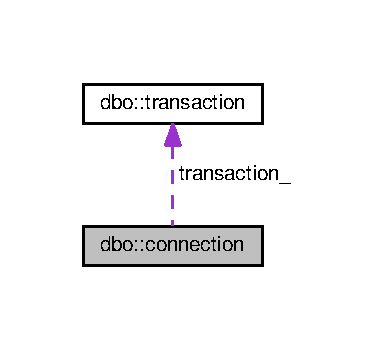
\includegraphics[width=180pt]{classdbo_1_1connection__coll__graph}
\end{center}
\end{figure}
\subsection*{Classes}
\begin{DoxyCompactItemize}
\item 
struct \hyperlink{structdbo_1_1connection_1_1typecomp}{typecomp}
\end{DoxyCompactItemize}
\subsection*{Public Member Functions}
\begin{DoxyCompactItemize}
\item 
\hyperlink{classdbo_1_1connection_abf4fbe074e578b5744dc6dc8e595d8e8}{connection} ()
\item 
virtual \hyperlink{classdbo_1_1connection_a974638af9e9e1e5659dee7c9fab326ed}{$\sim$connection} ()
\item 
void \hyperlink{classdbo_1_1connection_aae5734a1ebadaf2597d9172c5ab7115a}{connect} (std\+::string options=\char`\"{}\char`\"{})
\begin{DoxyCompactList}\small\item\em Connects to database. $\ast$. \end{DoxyCompactList}\item 
bool \hyperlink{classdbo_1_1connection_a1a68a49bf2ce826eaa08d1eb2527b454}{connected} () const 
\item 
{\footnotesize template$<$class C $>$ }\\void \hyperlink{classdbo_1_1connection_a78a8ab8b3fa23d45c96d75b906652e86}{map\+Class} (std\+::string name)
\begin{DoxyCompactList}\small\item\em Maps a class to a database table. \end{DoxyCompactList}\item 
{\footnotesize template$<$class C $>$ }\\const std\+::string \& \hyperlink{classdbo_1_1connection_ade1cbdc41769464cd1076e09c2099c9a}{table\+Name} () const 
\begin{DoxyCompactList}\small\item\em Returns the mapped table name for a class. \end{DoxyCompactList}\item 
void \hyperlink{classdbo_1_1connection_a35c81eabb228750f0e4c517eb63d6de2}{create\+Tables} ()
\begin{DoxyCompactList}\small\item\em Creates the database schema. \end{DoxyCompactList}\item 
std\+::string \hyperlink{classdbo_1_1connection_a5105d77e3a30044c0a97cdd42c8dbc62}{table\+Creation\+Sql} ()
\begin{DoxyCompactList}\small\item\em Returns database creation S\+Q\+L. \end{DoxyCompactList}\item 
\hyperlink{classdbo_1_1transaction}{dbo\+::transaction} \& \hyperlink{classdbo_1_1connection_a9e5653a2fc346acae23be6c3fd64e6aa}{transaction} ()
\item 
void \hyperlink{classdbo_1_1connection_a4ca7a503bc8fc3373ac2e49ea9c53f8f}{transaction} (std\+::function$<$ void()$>$ func)
\item 
{\footnotesize template$<$class C $>$ }\\\hyperlink{classdbo_1_1ptr}{ptr}$<$ C $>$ \& \hyperlink{classdbo_1_1connection_a9aee3a878ec49c35c6c51caf608a830f}{insert} (\hyperlink{classdbo_1_1ptr}{ptr}$<$ C $>$ \&\hyperlink{classdbo_1_1ptr}{ptr}, \hyperlink{classdbo_1_1_action_option}{Action\+Option} opt=\hyperlink{namespacedbo_1_1opt_ab4b7820471aaf46d67dffc2ee8b91dc4}{opt\+::\+None})
\item 
{\footnotesize template$<$class C $>$ }\\\hyperlink{classdbo_1_1collection}{collection}$<$ C $>$ \& \hyperlink{classdbo_1_1connection_ad89a1897d616931d30d9fd8d1258a9ca}{insert} (\hyperlink{classdbo_1_1collection}{collection}$<$ C $>$ \&coll, \hyperlink{classdbo_1_1_action_option}{Action\+Option} opt=\hyperlink{namespacedbo_1_1opt_ab4b7820471aaf46d67dffc2ee8b91dc4}{opt\+::\+None})
\item 
{\footnotesize template$<$class C $>$ }\\\hyperlink{classdbo_1_1ptr}{ptr}$<$ C $>$ \hyperlink{classdbo_1_1connection_a715d6c6defb04ba52aa09b630a0690a0}{update} (\hyperlink{classdbo_1_1ptr}{ptr}$<$ C $>$ \&\hyperlink{classdbo_1_1ptr}{ptr})
\item 
{\footnotesize template$<$class C $>$ }\\\hyperlink{classdbo_1_1ptr}{ptr}$<$ C $>$ \hyperlink{classdbo_1_1connection_a2543fa651e2588cc33c8609006ea9f75}{load} (\hyperlink{classdbo_1_1ptr}{ptr}$<$ C $>$ \&\hyperlink{classdbo_1_1ptr}{ptr})
\item 
{\footnotesize template$<$class C $>$ }\\\hyperlink{classdbo_1_1ptr}{ptr}$<$ C $>$ \hyperlink{classdbo_1_1connection_a877e459a53832d28340a58b41faafe38}{load} (const typename \hyperlink{structdbo_1_1traits_1_1dbo__traits}{traits\+::dbo\+\_\+traits}$<$ C $>$\+::Id\+Type \&\hyperlink{namespacedbo_a8d25907296ae8360b3120b7492022c1d}{id})
\item 
{\footnotesize template$<$class C $>$ }\\void \hyperlink{classdbo_1_1connection_a6943a85362796da5b6a054e680817d34}{remove} (\hyperlink{classdbo_1_1ptr}{ptr}$<$ C $>$ \&\hyperlink{classdbo_1_1ptr}{ptr})
\item 
{\footnotesize template$<$class C $>$ }\\\hyperlink{classdbo_1_1query}{query} \hyperlink{classdbo_1_1connection_add07b767b4b22afb986babf8dd899b65}{find} (const std\+::string \&condition=\char`\"{}\char`\"{})
\item 
{\footnotesize template$<$class C $>$ }\\\hyperlink{classdbo_1_1query}{query} \hyperlink{classdbo_1_1connection_a77a4ae27ad8ead0540ecb777f75bd019}{find} (const \hyperlink{classdbo_1_1collection}{collection}$<$ C $>$ \&\hyperlink{classdbo_1_1collection}{collection}, const std\+::string \&condition=\char`\"{}\char`\"{})
\item 
\hyperlink{classdbo_1_1query}{dbo\+::query} \hyperlink{classdbo_1_1connection_acdfefa09f01c05245667a982997ebbf3}{query} (const std\+::string \&sql)
\item 
void \hyperlink{classdbo_1_1connection_a69fbd222607d92d26f4982372a983e9e}{debug} ()
\item 
bool \hyperlink{classdbo_1_1connection_ac7e8bf86476f50eb3206b02c2d630b57}{show\+Queries} () const 
\item 
void \hyperlink{classdbo_1_1connection_a7fc0f5d76e19b92fb2d496ce28f033e9}{show\+Queries} (bool value)
\item 
bool \hyperlink{classdbo_1_1connection_ae869e5469a63b2db3e4b8eddf182d62b}{show\+Bindings} () const 
\item 
void \hyperlink{classdbo_1_1connection_acf2c95c516bce9b9086b69498bff4515}{show\+Bindings} (bool value)
\item 
bool \hyperlink{classdbo_1_1connection_a56fb518379af8d6930c15fb00390b80d}{show\+Results} () const 
\item 
void \hyperlink{classdbo_1_1connection_ad976083297b76e9ccd62e88fb4e79e7e}{show\+Results} (bool value)
\end{DoxyCompactItemize}
\subsection*{Protected Types}
\begin{DoxyCompactItemize}
\item 
typedef const std\+::type\+\_\+info $\ast$ \hyperlink{classdbo_1_1connection_ad9b28dcf5699796d552af8a159f03a5a}{const\+\_\+typeinfo\+\_\+ptr}
\item 
using \hyperlink{classdbo_1_1connection_acca03a784c87ffb1ec7bdf33f526dff5}{Mapping\+Info\+Ptr} = std\+::shared\+\_\+ptr$<$ \hyperlink{classdbo_1_1mapping_1_1_mapping_info}{mapping\+::\+Mapping\+Info} $>$
\item 
using \hyperlink{classdbo_1_1connection_adecb3694055470fb13f96185f3804e4e}{Class\+Registry} = std\+::map$<$ \hyperlink{classdbo_1_1connection_ad9b28dcf5699796d552af8a159f03a5a}{const\+\_\+typeinfo\+\_\+ptr}, \hyperlink{classdbo_1_1connection_acca03a784c87ffb1ec7bdf33f526dff5}{Mapping\+Info\+Ptr}, \hyperlink{structdbo_1_1connection_1_1typecomp}{typecomp} $>$
\item 
using \hyperlink{classdbo_1_1connection_ac58484f4b88dbc57cbd1f63471aa456d}{Table\+Registry} = std\+::unordered\+\_\+map$<$ std\+::string, \hyperlink{classdbo_1_1connection_acca03a784c87ffb1ec7bdf33f526dff5}{Mapping\+Info\+Ptr} $>$
\item 
using \hyperlink{classdbo_1_1connection_a14300ab905d89431e1410f657c10f217}{Types} = \hyperlink{classdbo_1_1traits_1_1_sql_postgres_types}{traits\+::\+Sql\+Postgres\+Types}
\end{DoxyCompactItemize}
\subsection*{Protected Member Functions}
\begin{DoxyCompactItemize}
\item 
void \hyperlink{classdbo_1_1connection_a20dfa44b7e33cc6c7e4608153ee858aa}{execute\+Sql} (const std\+::vector$<$ std\+::string $>$ \&sql, std\+::ostream $\ast$sout=nullptr)
\item 
void \hyperlink{classdbo_1_1connection_ac0145aacaaf4825b30f4d5658c3e1a99}{execute\+Sql} (const std\+::stringstream \&sql, std\+::ostream $\ast$sout=nullptr)
\item 
void \hyperlink{classdbo_1_1connection_a367170bd3ee09486b2b98dc744865122}{execute\+Sql} (const std\+::string \&sql, std\+::ostream $\ast$sout=nullptr)
\item 
void \hyperlink{classdbo_1_1connection_a5b21d06d9dbd4d26c0e45f3e9d8d858e}{resolve\+Join\+Ids} (\hyperlink{classdbo_1_1connection_acca03a784c87ffb1ec7bdf33f526dff5}{Mapping\+Info\+Ptr} mapping)
\item 
void \hyperlink{classdbo_1_1connection_a4ff08bfe57ea4e7f57ad18882da3318b}{create\+Relations} (\hyperlink{classdbo_1_1connection_acca03a784c87ffb1ec7bdf33f526dff5}{Mapping\+Info\+Ptr} mapping, std\+::set$<$ std\+::string $>$ \&tables\+Created, std\+::ostream $\ast$sout)
\item 
void \hyperlink{classdbo_1_1connection_a6e2ae3d9b23274bdf55dd1b703cce598}{init\+Schema} ()
\item 
void \hyperlink{classdbo_1_1connection_aab0c16df3bda31c2efbf9ee6a4ef8a60}{create\+Table} (\hyperlink{classdbo_1_1connection_acca03a784c87ffb1ec7bdf33f526dff5}{Mapping\+Info\+Ptr} mapping, std\+::set$<$ std\+::string $>$ \&tables\+Created, std\+::ostream $\ast$sout, bool create\+Constraints)
\item 
std\+::string \hyperlink{classdbo_1_1connection_a062d5ba43ddd69a9ba8efa4141df2b8b}{constraint\+String} (\hyperlink{classdbo_1_1connection_acca03a784c87ffb1ec7bdf33f526dff5}{Mapping\+Info\+Ptr} mapping, const \hyperlink{classdbo_1_1mapping_1_1_field_info}{mapping\+::\+Field\+Info} \&\hyperlink{namespacedbo_ad1f50f02cb050acf946807959252a93f}{field}, unsigned from\+Index, unsigned to\+Index)
\item 
unsigned \hyperlink{classdbo_1_1connection_ab7e69a0ef59496131688eebdedba1827}{find\+Last\+Foreign\+Key\+Field} (\hyperlink{classdbo_1_1connection_acca03a784c87ffb1ec7bdf33f526dff5}{Mapping\+Info\+Ptr} mapping, const \hyperlink{classdbo_1_1mapping_1_1_field_info}{mapping\+::\+Field\+Info} \&\hyperlink{namespacedbo_ad1f50f02cb050acf946807959252a93f}{field}, unsigned index)
\item 
void \hyperlink{classdbo_1_1connection_a392f2f9b92b477aac4c61ed23f3f3671}{create\+Join\+Table} (const std\+::string \&join\+Name, \hyperlink{classdbo_1_1connection_acca03a784c87ffb1ec7bdf33f526dff5}{Mapping\+Info\+Ptr} mapping1, \hyperlink{classdbo_1_1connection_acca03a784c87ffb1ec7bdf33f526dff5}{Mapping\+Info\+Ptr} mapping2, const std\+::string \&join\+Id1, const std\+::string \&join\+Id2, int fk\+Constraints1, int fk\+Constraints2, std\+::set$<$ std\+::string $>$ \&tables\+Created, std\+::ostream $\ast$sout)
\item 
std\+::vector$<$ \hyperlink{structdbo_1_1mapping_1_1_join_id}{mapping\+::\+Join\+Id} $>$ \hyperlink{classdbo_1_1connection_a73cc012991e1f732b8f871ba8a36143c}{get\+Join\+Ids} (\hyperlink{classdbo_1_1connection_acca03a784c87ffb1ec7bdf33f526dff5}{Mapping\+Info\+Ptr} mapping, const std\+::string \&join\+Id)
\item 
void \hyperlink{classdbo_1_1connection_aa92e86aed48a4224501c7a2d3700d8d8}{add\+Join\+Table\+Fields} (\hyperlink{classdbo_1_1connection_acca03a784c87ffb1ec7bdf33f526dff5}{Mapping\+Info\+Ptr} result, \hyperlink{classdbo_1_1connection_acca03a784c87ffb1ec7bdf33f526dff5}{Mapping\+Info\+Ptr} mapping, const std\+::string \&join\+Id, const std\+::string \&key\+Name, int fk\+Constraints)
\item 
void \hyperlink{classdbo_1_1connection_ae8f0004c9e859c113918b5a8e766bb9e}{create\+Join\+Index} (\hyperlink{classdbo_1_1connection_acca03a784c87ffb1ec7bdf33f526dff5}{Mapping\+Info\+Ptr} join\+Table\+Mapping, \hyperlink{classdbo_1_1connection_acca03a784c87ffb1ec7bdf33f526dff5}{Mapping\+Info\+Ptr} mapping, const std\+::string \&join\+Id, const std\+::string \&foreign\+Key\+Name, std\+::ostream $\ast$sout)
\item 
void \hyperlink{classdbo_1_1connection_a73872df92d7ecfbdc57c8d8c1798392c}{prepare\+Insert\+Statements} (\hyperlink{classdbo_1_1connection_acca03a784c87ffb1ec7bdf33f526dff5}{Mapping\+Info\+Ptr} mapping)
\item 
void \hyperlink{classdbo_1_1connection_a0b6721462bddeb5349838e498e0ea839}{prepare\+Update\+Statements} (\hyperlink{classdbo_1_1connection_acca03a784c87ffb1ec7bdf33f526dff5}{Mapping\+Info\+Ptr} mapping)
\item 
void \hyperlink{classdbo_1_1connection_a7b9e24007952236d77dfabba20617e75}{prepare\+Delete\+Statements} (\hyperlink{classdbo_1_1connection_acca03a784c87ffb1ec7bdf33f526dff5}{Mapping\+Info\+Ptr} mapping)
\item 
void \hyperlink{classdbo_1_1connection_aa0953ba22e1fb34a7e80e557e117904f}{prepare\+Selected\+By\+Id\+Statements} (\hyperlink{classdbo_1_1connection_acca03a784c87ffb1ec7bdf33f526dff5}{Mapping\+Info\+Ptr} mapping)
\item 
void \hyperlink{classdbo_1_1connection_a3a73f471795ea5dee870f5ee3b51c1b6}{prepare\+Collections\+Statements} (\hyperlink{classdbo_1_1connection_acca03a784c87ffb1ec7bdf33f526dff5}{Mapping\+Info\+Ptr} mapping)
\item 
void \hyperlink{classdbo_1_1connection_a1c878e83c11f7f524920620e692cb61f}{prepare\+Statements} (\hyperlink{classdbo_1_1connection_acca03a784c87ffb1ec7bdf33f526dff5}{Mapping\+Info\+Ptr} mapping)
\item 
{\footnotesize template$<$class C $>$ }\\std\+::shared\+\_\+ptr\\*
$<$ \hyperlink{classdbo_1_1mapping_1_1_mapping}{mapping\+::\+Mapping}$<$ C $>$ $>$ \hyperlink{classdbo_1_1connection_ad29f174ef8539b4e3ae60c91a293adf8}{get\+Mapping} ()
\item 
\hyperlink{classdbo_1_1connection_acca03a784c87ffb1ec7bdf33f526dff5}{Mapping\+Info\+Ptr} \hyperlink{classdbo_1_1connection_a94500555db4f80aef65861c5ff9e6c10}{get\+Mapping} (const std\+::string \&\hyperlink{classdbo_1_1connection_ade1cbdc41769464cd1076e09c2099c9a}{table\+Name}) const 
\end{DoxyCompactItemize}
\subsection*{Protected Attributes}
\begin{DoxyCompactItemize}
\item 
std\+::string \hyperlink{classdbo_1_1connection_ab03d3dced341bf89b5cecdd645fff3d4}{options\+\_\+}
\item 
\hyperlink{connection_8h_a5ed62e34058025c39959695e724603a6}{P\+Gconn} $\ast$ \hyperlink{classdbo_1_1connection_a5bea8990337d86b92b274004a94288b4}{conn\+\_\+}
\item 
bool \hyperlink{classdbo_1_1connection_a38caab3883d4d165d0ef7fc81791dd95}{show\+Queries\+\_\+}
\item 
bool \hyperlink{classdbo_1_1connection_a1b14e416f52aed1aa46b9600bdd8c466}{show\+Bindings\+\_\+}
\item 
bool \hyperlink{classdbo_1_1connection_afdcf9d15e645a452153699e6833ea59f}{show\+Results\+\_\+}
\item 
bool \hyperlink{classdbo_1_1connection_aceadf42379584e3736187409857cff8f}{schema\+Initialized\+\_\+}
\item 
\hyperlink{classdbo_1_1connection_adecb3694055470fb13f96185f3804e4e}{Class\+Registry} \hyperlink{classdbo_1_1connection_a9dae61c756636fa11ad66de2b02d05aa}{class\+Registry\+\_\+}
\item 
\hyperlink{classdbo_1_1connection_ac58484f4b88dbc57cbd1f63471aa456d}{Table\+Registry} \hyperlink{classdbo_1_1connection_a9b17470dcf5f38ca668bd01852db2a52}{table\+Registry\+\_\+}
\item 
\hyperlink{classdbo_1_1transaction}{dbo\+::transaction} \hyperlink{classdbo_1_1connection_a7d822f46486566b7e6b310a581e6a148}{transaction\+\_\+}
\end{DoxyCompactItemize}
\subsection*{Friends}
\begin{DoxyCompactItemize}
\item 
{\footnotesize template$<$class T $>$ }\\class \hyperlink{classdbo_1_1connection_ae779179e16547c9a93329dd197385493}{action\+::\+Delete}
\item 
{\footnotesize template$<$class T $>$ }\\class \hyperlink{classdbo_1_1connection_a88a9b73e2cb3304941371508b660e53e}{action\+::\+Insert}
\item 
{\footnotesize template$<$class T $>$ }\\class \hyperlink{classdbo_1_1connection_a8b98481706995f8b3e2665f74b2b3039}{action\+::\+Select\+By\+Id}
\item 
{\footnotesize template$<$class T $>$ }\\class \hyperlink{classdbo_1_1connection_a90af99826aea472a0aa22e59376fed0f}{action\+::\+Update}
\item 
class \hyperlink{classdbo_1_1connection_af0423915055bedb88a9d6d44bd6d7d86}{action\+::\+Init\+Schema}
\item 
{\footnotesize template$<$class C $>$ }\\class \hyperlink{classdbo_1_1connection_a1dfe637f2baf477f4a0579512df51cf6}{mapping\+::\+Ptr\+Ref}
\item 
class \hyperlink{classdbo_1_1connection_afb842ec251d7985ea41205c003c9b86e}{stmt\+::\+Prepared\+Statement}
\item 
class \hyperlink{classdbo_1_1connection_ac67430204a570dc3ecd9da0db836157d}{stmt\+::\+Bulk\+Statement}
\item 
class \hyperlink{classdbo_1_1connection_a7fddf73eaed86e45a2aacbd26b5af751}{query}
\item 
class \hyperlink{classdbo_1_1connection_ac6311258cbfe9139b0ca828a99e9ce04}{transaction}
\end{DoxyCompactItemize}


\subsection{Member Typedef Documentation}
\hypertarget{classdbo_1_1connection_adecb3694055470fb13f96185f3804e4e}{\index{dbo\+::connection@{dbo\+::connection}!Class\+Registry@{Class\+Registry}}
\index{Class\+Registry@{Class\+Registry}!dbo\+::connection@{dbo\+::connection}}
\subsubsection[{Class\+Registry}]{\setlength{\rightskip}{0pt plus 5cm}using {\bf dbo\+::connection\+::\+Class\+Registry} =  std\+::map$<${\bf const\+\_\+typeinfo\+\_\+ptr}, {\bf Mapping\+Info\+Ptr}, {\bf typecomp}$>$\hspace{0.3cm}{\ttfamily [protected]}}}\label{classdbo_1_1connection_adecb3694055470fb13f96185f3804e4e}
\hypertarget{classdbo_1_1connection_ad9b28dcf5699796d552af8a159f03a5a}{\index{dbo\+::connection@{dbo\+::connection}!const\+\_\+typeinfo\+\_\+ptr@{const\+\_\+typeinfo\+\_\+ptr}}
\index{const\+\_\+typeinfo\+\_\+ptr@{const\+\_\+typeinfo\+\_\+ptr}!dbo\+::connection@{dbo\+::connection}}
\subsubsection[{const\+\_\+typeinfo\+\_\+ptr}]{\setlength{\rightskip}{0pt plus 5cm}typedef const std\+::type\+\_\+info$\ast$ {\bf dbo\+::connection\+::const\+\_\+typeinfo\+\_\+ptr}\hspace{0.3cm}{\ttfamily [protected]}}}\label{classdbo_1_1connection_ad9b28dcf5699796d552af8a159f03a5a}
\hypertarget{classdbo_1_1connection_acca03a784c87ffb1ec7bdf33f526dff5}{\index{dbo\+::connection@{dbo\+::connection}!Mapping\+Info\+Ptr@{Mapping\+Info\+Ptr}}
\index{Mapping\+Info\+Ptr@{Mapping\+Info\+Ptr}!dbo\+::connection@{dbo\+::connection}}
\subsubsection[{Mapping\+Info\+Ptr}]{\setlength{\rightskip}{0pt plus 5cm}using {\bf dbo\+::connection\+::\+Mapping\+Info\+Ptr} =  std\+::shared\+\_\+ptr$<${\bf mapping\+::\+Mapping\+Info}$>$\hspace{0.3cm}{\ttfamily [protected]}}}\label{classdbo_1_1connection_acca03a784c87ffb1ec7bdf33f526dff5}
\hypertarget{classdbo_1_1connection_ac58484f4b88dbc57cbd1f63471aa456d}{\index{dbo\+::connection@{dbo\+::connection}!Table\+Registry@{Table\+Registry}}
\index{Table\+Registry@{Table\+Registry}!dbo\+::connection@{dbo\+::connection}}
\subsubsection[{Table\+Registry}]{\setlength{\rightskip}{0pt plus 5cm}using {\bf dbo\+::connection\+::\+Table\+Registry} =  std\+::unordered\+\_\+map$<$std\+::string, {\bf Mapping\+Info\+Ptr}$>$\hspace{0.3cm}{\ttfamily [protected]}}}\label{classdbo_1_1connection_ac58484f4b88dbc57cbd1f63471aa456d}
\hypertarget{classdbo_1_1connection_a14300ab905d89431e1410f657c10f217}{\index{dbo\+::connection@{dbo\+::connection}!Types@{Types}}
\index{Types@{Types}!dbo\+::connection@{dbo\+::connection}}
\subsubsection[{Types}]{\setlength{\rightskip}{0pt plus 5cm}using {\bf dbo\+::connection\+::\+Types} =  {\bf traits\+::\+Sql\+Postgres\+Types}\hspace{0.3cm}{\ttfamily [protected]}}}\label{classdbo_1_1connection_a14300ab905d89431e1410f657c10f217}


\subsection{Constructor \& Destructor Documentation}
\hypertarget{classdbo_1_1connection_abf4fbe074e578b5744dc6dc8e595d8e8}{\index{dbo\+::connection@{dbo\+::connection}!connection@{connection}}
\index{connection@{connection}!dbo\+::connection@{dbo\+::connection}}
\subsubsection[{connection}]{\setlength{\rightskip}{0pt plus 5cm}connection\+::connection (
\begin{DoxyParamCaption}
{}
\end{DoxyParamCaption}
)}}\label{classdbo_1_1connection_abf4fbe074e578b5744dc6dc8e595d8e8}
\hypertarget{classdbo_1_1connection_a974638af9e9e1e5659dee7c9fab326ed}{\index{dbo\+::connection@{dbo\+::connection}!````~connection@{$\sim$connection}}
\index{````~connection@{$\sim$connection}!dbo\+::connection@{dbo\+::connection}}
\subsubsection[{$\sim$connection}]{\setlength{\rightskip}{0pt plus 5cm}connection\+::$\sim$connection (
\begin{DoxyParamCaption}
{}
\end{DoxyParamCaption}
)\hspace{0.3cm}{\ttfamily [virtual]}}}\label{classdbo_1_1connection_a974638af9e9e1e5659dee7c9fab326ed}


\subsection{Member Function Documentation}
\hypertarget{classdbo_1_1connection_aa92e86aed48a4224501c7a2d3700d8d8}{\index{dbo\+::connection@{dbo\+::connection}!add\+Join\+Table\+Fields@{add\+Join\+Table\+Fields}}
\index{add\+Join\+Table\+Fields@{add\+Join\+Table\+Fields}!dbo\+::connection@{dbo\+::connection}}
\subsubsection[{add\+Join\+Table\+Fields}]{\setlength{\rightskip}{0pt plus 5cm}void connection\+::add\+Join\+Table\+Fields (
\begin{DoxyParamCaption}
\item[{{\bf Mapping\+Info\+Ptr}}]{result, }
\item[{{\bf Mapping\+Info\+Ptr}}]{mapping, }
\item[{const std\+::string \&}]{join\+Id, }
\item[{const std\+::string \&}]{key\+Name, }
\item[{int}]{fk\+Constraints}
\end{DoxyParamCaption}
)\hspace{0.3cm}{\ttfamily [protected]}}}\label{classdbo_1_1connection_aa92e86aed48a4224501c7a2d3700d8d8}
\hypertarget{classdbo_1_1connection_aae5734a1ebadaf2597d9172c5ab7115a}{\index{dbo\+::connection@{dbo\+::connection}!connect@{connect}}
\index{connect@{connect}!dbo\+::connection@{dbo\+::connection}}
\subsubsection[{connect}]{\setlength{\rightskip}{0pt plus 5cm}void connection\+::connect (
\begin{DoxyParamCaption}
\item[{std\+::string}]{options = {\ttfamily \char`\"{}\char`\"{}}}
\end{DoxyParamCaption}
)}}\label{classdbo_1_1connection_aae5734a1ebadaf2597d9172c5ab7115a}


Connects to database. $\ast$. 

\hypertarget{classdbo_1_1connection_a1a68a49bf2ce826eaa08d1eb2527b454}{\index{dbo\+::connection@{dbo\+::connection}!connected@{connected}}
\index{connected@{connected}!dbo\+::connection@{dbo\+::connection}}
\subsubsection[{connected}]{\setlength{\rightskip}{0pt plus 5cm}bool connection\+::connected (
\begin{DoxyParamCaption}
{}
\end{DoxyParamCaption}
) const}}\label{classdbo_1_1connection_a1a68a49bf2ce826eaa08d1eb2527b454}
\hypertarget{classdbo_1_1connection_a062d5ba43ddd69a9ba8efa4141df2b8b}{\index{dbo\+::connection@{dbo\+::connection}!constraint\+String@{constraint\+String}}
\index{constraint\+String@{constraint\+String}!dbo\+::connection@{dbo\+::connection}}
\subsubsection[{constraint\+String}]{\setlength{\rightskip}{0pt plus 5cm}std\+::string connection\+::constraint\+String (
\begin{DoxyParamCaption}
\item[{{\bf Mapping\+Info\+Ptr}}]{mapping, }
\item[{const {\bf mapping\+::\+Field\+Info} \&}]{field, }
\item[{unsigned}]{from\+Index, }
\item[{unsigned}]{to\+Index}
\end{DoxyParamCaption}
)\hspace{0.3cm}{\ttfamily [protected]}}}\label{classdbo_1_1connection_a062d5ba43ddd69a9ba8efa4141df2b8b}
\hypertarget{classdbo_1_1connection_ae8f0004c9e859c113918b5a8e766bb9e}{\index{dbo\+::connection@{dbo\+::connection}!create\+Join\+Index@{create\+Join\+Index}}
\index{create\+Join\+Index@{create\+Join\+Index}!dbo\+::connection@{dbo\+::connection}}
\subsubsection[{create\+Join\+Index}]{\setlength{\rightskip}{0pt plus 5cm}void connection\+::create\+Join\+Index (
\begin{DoxyParamCaption}
\item[{{\bf Mapping\+Info\+Ptr}}]{join\+Table\+Mapping, }
\item[{{\bf Mapping\+Info\+Ptr}}]{mapping, }
\item[{const std\+::string \&}]{join\+Id, }
\item[{const std\+::string \&}]{foreign\+Key\+Name, }
\item[{std\+::ostream $\ast$}]{sout}
\end{DoxyParamCaption}
)\hspace{0.3cm}{\ttfamily [protected]}}}\label{classdbo_1_1connection_ae8f0004c9e859c113918b5a8e766bb9e}
\hypertarget{classdbo_1_1connection_a392f2f9b92b477aac4c61ed23f3f3671}{\index{dbo\+::connection@{dbo\+::connection}!create\+Join\+Table@{create\+Join\+Table}}
\index{create\+Join\+Table@{create\+Join\+Table}!dbo\+::connection@{dbo\+::connection}}
\subsubsection[{create\+Join\+Table}]{\setlength{\rightskip}{0pt plus 5cm}void connection\+::create\+Join\+Table (
\begin{DoxyParamCaption}
\item[{const std\+::string \&}]{join\+Name, }
\item[{{\bf Mapping\+Info\+Ptr}}]{mapping1, }
\item[{{\bf Mapping\+Info\+Ptr}}]{mapping2, }
\item[{const std\+::string \&}]{join\+Id1, }
\item[{const std\+::string \&}]{join\+Id2, }
\item[{int}]{fk\+Constraints1, }
\item[{int}]{fk\+Constraints2, }
\item[{std\+::set$<$ std\+::string $>$ \&}]{tables\+Created, }
\item[{std\+::ostream $\ast$}]{sout}
\end{DoxyParamCaption}
)\hspace{0.3cm}{\ttfamily [protected]}}}\label{classdbo_1_1connection_a392f2f9b92b477aac4c61ed23f3f3671}
\hypertarget{classdbo_1_1connection_a4ff08bfe57ea4e7f57ad18882da3318b}{\index{dbo\+::connection@{dbo\+::connection}!create\+Relations@{create\+Relations}}
\index{create\+Relations@{create\+Relations}!dbo\+::connection@{dbo\+::connection}}
\subsubsection[{create\+Relations}]{\setlength{\rightskip}{0pt plus 5cm}void connection\+::create\+Relations (
\begin{DoxyParamCaption}
\item[{{\bf Mapping\+Info\+Ptr}}]{mapping, }
\item[{std\+::set$<$ std\+::string $>$ \&}]{tables\+Created, }
\item[{std\+::ostream $\ast$}]{sout}
\end{DoxyParamCaption}
)\hspace{0.3cm}{\ttfamily [protected]}}}\label{classdbo_1_1connection_a4ff08bfe57ea4e7f57ad18882da3318b}
\hypertarget{classdbo_1_1connection_aab0c16df3bda31c2efbf9ee6a4ef8a60}{\index{dbo\+::connection@{dbo\+::connection}!create\+Table@{create\+Table}}
\index{create\+Table@{create\+Table}!dbo\+::connection@{dbo\+::connection}}
\subsubsection[{create\+Table}]{\setlength{\rightskip}{0pt plus 5cm}void connection\+::create\+Table (
\begin{DoxyParamCaption}
\item[{{\bf Mapping\+Info\+Ptr}}]{mapping, }
\item[{std\+::set$<$ std\+::string $>$ \&}]{tables\+Created, }
\item[{std\+::ostream $\ast$}]{sout, }
\item[{bool}]{create\+Constraints}
\end{DoxyParamCaption}
)\hspace{0.3cm}{\ttfamily [protected]}}}\label{classdbo_1_1connection_aab0c16df3bda31c2efbf9ee6a4ef8a60}
\hypertarget{classdbo_1_1connection_a35c81eabb228750f0e4c517eb63d6de2}{\index{dbo\+::connection@{dbo\+::connection}!create\+Tables@{create\+Tables}}
\index{create\+Tables@{create\+Tables}!dbo\+::connection@{dbo\+::connection}}
\subsubsection[{create\+Tables}]{\setlength{\rightskip}{0pt plus 5cm}void connection\+::create\+Tables (
\begin{DoxyParamCaption}
{}
\end{DoxyParamCaption}
)}}\label{classdbo_1_1connection_a35c81eabb228750f0e4c517eb63d6de2}


Creates the database schema. 

This will create the database schema of the mapped tables. Schema creation will fail if one or more tables already existed. The creation of the tables is executed in a transaction that is rolled back when an error occurs.

This method throws an \hyperlink{classdbo_1_1_exception}{dbo\+::\+Exception} if the table creation failed.

\begin{DoxySeeAlso}{See also}
\hyperlink{classdbo_1_1connection_a78a8ab8b3fa23d45c96d75b906652e86}{map\+Class()}, drop\+Tables() 
\end{DoxySeeAlso}
\hypertarget{classdbo_1_1connection_a69fbd222607d92d26f4982372a983e9e}{\index{dbo\+::connection@{dbo\+::connection}!debug@{debug}}
\index{debug@{debug}!dbo\+::connection@{dbo\+::connection}}
\subsubsection[{debug}]{\setlength{\rightskip}{0pt plus 5cm}void connection\+::debug (
\begin{DoxyParamCaption}
{}
\end{DoxyParamCaption}
)}}\label{classdbo_1_1connection_a69fbd222607d92d26f4982372a983e9e}
\hypertarget{classdbo_1_1connection_a20dfa44b7e33cc6c7e4608153ee858aa}{\index{dbo\+::connection@{dbo\+::connection}!execute\+Sql@{execute\+Sql}}
\index{execute\+Sql@{execute\+Sql}!dbo\+::connection@{dbo\+::connection}}
\subsubsection[{execute\+Sql}]{\setlength{\rightskip}{0pt plus 5cm}void connection\+::execute\+Sql (
\begin{DoxyParamCaption}
\item[{const std\+::vector$<$ std\+::string $>$ \&}]{sql, }
\item[{std\+::ostream $\ast$}]{sout = {\ttfamily nullptr}}
\end{DoxyParamCaption}
)\hspace{0.3cm}{\ttfamily [protected]}}}\label{classdbo_1_1connection_a20dfa44b7e33cc6c7e4608153ee858aa}
\hypertarget{classdbo_1_1connection_ac0145aacaaf4825b30f4d5658c3e1a99}{\index{dbo\+::connection@{dbo\+::connection}!execute\+Sql@{execute\+Sql}}
\index{execute\+Sql@{execute\+Sql}!dbo\+::connection@{dbo\+::connection}}
\subsubsection[{execute\+Sql}]{\setlength{\rightskip}{0pt plus 5cm}void connection\+::execute\+Sql (
\begin{DoxyParamCaption}
\item[{const std\+::stringstream \&}]{sql, }
\item[{std\+::ostream $\ast$}]{sout = {\ttfamily nullptr}}
\end{DoxyParamCaption}
)\hspace{0.3cm}{\ttfamily [protected]}}}\label{classdbo_1_1connection_ac0145aacaaf4825b30f4d5658c3e1a99}
\hypertarget{classdbo_1_1connection_a367170bd3ee09486b2b98dc744865122}{\index{dbo\+::connection@{dbo\+::connection}!execute\+Sql@{execute\+Sql}}
\index{execute\+Sql@{execute\+Sql}!dbo\+::connection@{dbo\+::connection}}
\subsubsection[{execute\+Sql}]{\setlength{\rightskip}{0pt plus 5cm}void connection\+::execute\+Sql (
\begin{DoxyParamCaption}
\item[{const std\+::string \&}]{sql, }
\item[{std\+::ostream $\ast$}]{sout = {\ttfamily nullptr}}
\end{DoxyParamCaption}
)\hspace{0.3cm}{\ttfamily [protected]}}}\label{classdbo_1_1connection_a367170bd3ee09486b2b98dc744865122}
\hypertarget{classdbo_1_1connection_add07b767b4b22afb986babf8dd899b65}{\index{dbo\+::connection@{dbo\+::connection}!find@{find}}
\index{find@{find}!dbo\+::connection@{dbo\+::connection}}
\subsubsection[{find}]{\setlength{\rightskip}{0pt plus 5cm}template$<$class C $>$ {\bf query} dbo\+::connection\+::find (
\begin{DoxyParamCaption}
\item[{const std\+::string \&}]{condition = {\ttfamily \char`\"{}\char`\"{}}}
\end{DoxyParamCaption}
)}}\label{classdbo_1_1connection_add07b767b4b22afb986babf8dd899b65}
Create a select query from mapping \hypertarget{classdbo_1_1connection_a77a4ae27ad8ead0540ecb777f75bd019}{\index{dbo\+::connection@{dbo\+::connection}!find@{find}}
\index{find@{find}!dbo\+::connection@{dbo\+::connection}}
\subsubsection[{find}]{\setlength{\rightskip}{0pt plus 5cm}template$<$class C $>$ {\bf query} dbo\+::connection\+::find (
\begin{DoxyParamCaption}
\item[{const {\bf collection}$<$ C $>$ \&}]{collection, }
\item[{const std\+::string \&}]{condition = {\ttfamily \char`\"{}\char`\"{}}}
\end{DoxyParamCaption}
)}}\label{classdbo_1_1connection_a77a4ae27ad8ead0540ecb777f75bd019}
Create a select query from collection mapping \hypertarget{classdbo_1_1connection_ab7e69a0ef59496131688eebdedba1827}{\index{dbo\+::connection@{dbo\+::connection}!find\+Last\+Foreign\+Key\+Field@{find\+Last\+Foreign\+Key\+Field}}
\index{find\+Last\+Foreign\+Key\+Field@{find\+Last\+Foreign\+Key\+Field}!dbo\+::connection@{dbo\+::connection}}
\subsubsection[{find\+Last\+Foreign\+Key\+Field}]{\setlength{\rightskip}{0pt plus 5cm}unsigned connection\+::find\+Last\+Foreign\+Key\+Field (
\begin{DoxyParamCaption}
\item[{{\bf Mapping\+Info\+Ptr}}]{mapping, }
\item[{const {\bf mapping\+::\+Field\+Info} \&}]{field, }
\item[{unsigned}]{index}
\end{DoxyParamCaption}
)\hspace{0.3cm}{\ttfamily [protected]}}}\label{classdbo_1_1connection_ab7e69a0ef59496131688eebdedba1827}
\hypertarget{classdbo_1_1connection_a73cc012991e1f732b8f871ba8a36143c}{\index{dbo\+::connection@{dbo\+::connection}!get\+Join\+Ids@{get\+Join\+Ids}}
\index{get\+Join\+Ids@{get\+Join\+Ids}!dbo\+::connection@{dbo\+::connection}}
\subsubsection[{get\+Join\+Ids}]{\setlength{\rightskip}{0pt plus 5cm}std\+::vector$<$ {\bf mapping\+::\+Join\+Id} $>$ connection\+::get\+Join\+Ids (
\begin{DoxyParamCaption}
\item[{{\bf Mapping\+Info\+Ptr}}]{mapping, }
\item[{const std\+::string \&}]{join\+Id}
\end{DoxyParamCaption}
)\hspace{0.3cm}{\ttfamily [protected]}}}\label{classdbo_1_1connection_a73cc012991e1f732b8f871ba8a36143c}
\hypertarget{classdbo_1_1connection_ad29f174ef8539b4e3ae60c91a293adf8}{\index{dbo\+::connection@{dbo\+::connection}!get\+Mapping@{get\+Mapping}}
\index{get\+Mapping@{get\+Mapping}!dbo\+::connection@{dbo\+::connection}}
\subsubsection[{get\+Mapping}]{\setlength{\rightskip}{0pt plus 5cm}template$<$class C $>$ std\+::shared\+\_\+ptr$<$ {\bf mapping\+::\+Mapping}$<$ C $>$ $>$ dbo\+::connection\+::get\+Mapping (
\begin{DoxyParamCaption}
{}
\end{DoxyParamCaption}
)\hspace{0.3cm}{\ttfamily [protected]}}}\label{classdbo_1_1connection_ad29f174ef8539b4e3ae60c91a293adf8}
\hypertarget{classdbo_1_1connection_a94500555db4f80aef65861c5ff9e6c10}{\index{dbo\+::connection@{dbo\+::connection}!get\+Mapping@{get\+Mapping}}
\index{get\+Mapping@{get\+Mapping}!dbo\+::connection@{dbo\+::connection}}
\subsubsection[{get\+Mapping}]{\setlength{\rightskip}{0pt plus 5cm}{\bf connection\+::\+Mapping\+Info\+Ptr} connection\+::get\+Mapping (
\begin{DoxyParamCaption}
\item[{const std\+::string \&}]{table\+Name}
\end{DoxyParamCaption}
) const\hspace{0.3cm}{\ttfamily [protected]}}}\label{classdbo_1_1connection_a94500555db4f80aef65861c5ff9e6c10}
\hypertarget{classdbo_1_1connection_a6e2ae3d9b23274bdf55dd1b703cce598}{\index{dbo\+::connection@{dbo\+::connection}!init\+Schema@{init\+Schema}}
\index{init\+Schema@{init\+Schema}!dbo\+::connection@{dbo\+::connection}}
\subsubsection[{init\+Schema}]{\setlength{\rightskip}{0pt plus 5cm}void connection\+::init\+Schema (
\begin{DoxyParamCaption}
{}
\end{DoxyParamCaption}
)\hspace{0.3cm}{\ttfamily [protected]}}}\label{classdbo_1_1connection_a6e2ae3d9b23274bdf55dd1b703cce598}
\hypertarget{classdbo_1_1connection_a9aee3a878ec49c35c6c51caf608a830f}{\index{dbo\+::connection@{dbo\+::connection}!insert@{insert}}
\index{insert@{insert}!dbo\+::connection@{dbo\+::connection}}
\subsubsection[{insert}]{\setlength{\rightskip}{0pt plus 5cm}template$<$class C $>$ {\bf ptr}$<$ C $>$ \& dbo\+::connection\+::insert (
\begin{DoxyParamCaption}
\item[{{\bf ptr}$<$ C $>$ \&}]{ptr, }
\item[{{\bf Action\+Option}}]{opt = {\ttfamily {\bf opt\+::\+None}}}
\end{DoxyParamCaption}
)}}\label{classdbo_1_1connection_a9aee3a878ec49c35c6c51caf608a830f}
Persists an object inside database and attribute it an id \hypertarget{classdbo_1_1connection_ad89a1897d616931d30d9fd8d1258a9ca}{\index{dbo\+::connection@{dbo\+::connection}!insert@{insert}}
\index{insert@{insert}!dbo\+::connection@{dbo\+::connection}}
\subsubsection[{insert}]{\setlength{\rightskip}{0pt plus 5cm}template$<$class C $>$ {\bf collection}$<$ C $>$ \& dbo\+::connection\+::insert (
\begin{DoxyParamCaption}
\item[{{\bf collection}$<$ C $>$ \&}]{coll, }
\item[{{\bf Action\+Option}}]{opt = {\ttfamily {\bf opt\+::\+None}}}
\end{DoxyParamCaption}
)}}\label{classdbo_1_1connection_ad89a1897d616931d30d9fd8d1258a9ca}
bulk insert content of collection \hypertarget{classdbo_1_1connection_a2543fa651e2588cc33c8609006ea9f75}{\index{dbo\+::connection@{dbo\+::connection}!load@{load}}
\index{load@{load}!dbo\+::connection@{dbo\+::connection}}
\subsubsection[{load}]{\setlength{\rightskip}{0pt plus 5cm}template$<$class C $>$ {\bf ptr}$<$ C $>$ dbo\+::connection\+::load (
\begin{DoxyParamCaption}
\item[{{\bf ptr}$<$ C $>$ \&}]{ptr}
\end{DoxyParamCaption}
)}}\label{classdbo_1_1connection_a2543fa651e2588cc33c8609006ea9f75}
Reload an existing object from database \hypertarget{classdbo_1_1connection_a877e459a53832d28340a58b41faafe38}{\index{dbo\+::connection@{dbo\+::connection}!load@{load}}
\index{load@{load}!dbo\+::connection@{dbo\+::connection}}
\subsubsection[{load}]{\setlength{\rightskip}{0pt plus 5cm}template$<$class C $>$ {\bf ptr}$<$ C $>$ dbo\+::connection\+::load (
\begin{DoxyParamCaption}
\item[{const typename {\bf traits\+::dbo\+\_\+traits}$<$ C $>$\+::Id\+Type \&}]{id}
\end{DoxyParamCaption}
)}}\label{classdbo_1_1connection_a877e459a53832d28340a58b41faafe38}
Load an object from database \hypertarget{classdbo_1_1connection_a78a8ab8b3fa23d45c96d75b906652e86}{\index{dbo\+::connection@{dbo\+::connection}!map\+Class@{map\+Class}}
\index{map\+Class@{map\+Class}!dbo\+::connection@{dbo\+::connection}}
\subsubsection[{map\+Class}]{\setlength{\rightskip}{0pt plus 5cm}template$<$class C $>$ void dbo\+::connection\+::map\+Class (
\begin{DoxyParamCaption}
\item[{std\+::string}]{name}
\end{DoxyParamCaption}
)}}\label{classdbo_1_1connection_a78a8ab8b3fa23d45c96d75b906652e86}


Maps a class to a database table. 

The class {\ttfamily C} is mapped to table with {\ttfamily table\+Name}. You need to map classes to tables.

You may provide a schema-\/qualified table name, if the underlying database supports this, eg. {\ttfamily \char`\"{}myschema.\+users\char`\"{}}. \hypertarget{classdbo_1_1connection_a3a73f471795ea5dee870f5ee3b51c1b6}{\index{dbo\+::connection@{dbo\+::connection}!prepare\+Collections\+Statements@{prepare\+Collections\+Statements}}
\index{prepare\+Collections\+Statements@{prepare\+Collections\+Statements}!dbo\+::connection@{dbo\+::connection}}
\subsubsection[{prepare\+Collections\+Statements}]{\setlength{\rightskip}{0pt plus 5cm}void connection\+::prepare\+Collections\+Statements (
\begin{DoxyParamCaption}
\item[{{\bf Mapping\+Info\+Ptr}}]{mapping}
\end{DoxyParamCaption}
)\hspace{0.3cm}{\ttfamily [protected]}}}\label{classdbo_1_1connection_a3a73f471795ea5dee870f5ee3b51c1b6}
\hypertarget{classdbo_1_1connection_a7b9e24007952236d77dfabba20617e75}{\index{dbo\+::connection@{dbo\+::connection}!prepare\+Delete\+Statements@{prepare\+Delete\+Statements}}
\index{prepare\+Delete\+Statements@{prepare\+Delete\+Statements}!dbo\+::connection@{dbo\+::connection}}
\subsubsection[{prepare\+Delete\+Statements}]{\setlength{\rightskip}{0pt plus 5cm}void connection\+::prepare\+Delete\+Statements (
\begin{DoxyParamCaption}
\item[{{\bf Mapping\+Info\+Ptr}}]{mapping}
\end{DoxyParamCaption}
)\hspace{0.3cm}{\ttfamily [protected]}}}\label{classdbo_1_1connection_a7b9e24007952236d77dfabba20617e75}
\hypertarget{classdbo_1_1connection_a73872df92d7ecfbdc57c8d8c1798392c}{\index{dbo\+::connection@{dbo\+::connection}!prepare\+Insert\+Statements@{prepare\+Insert\+Statements}}
\index{prepare\+Insert\+Statements@{prepare\+Insert\+Statements}!dbo\+::connection@{dbo\+::connection}}
\subsubsection[{prepare\+Insert\+Statements}]{\setlength{\rightskip}{0pt plus 5cm}void connection\+::prepare\+Insert\+Statements (
\begin{DoxyParamCaption}
\item[{{\bf Mapping\+Info\+Ptr}}]{mapping}
\end{DoxyParamCaption}
)\hspace{0.3cm}{\ttfamily [protected]}}}\label{classdbo_1_1connection_a73872df92d7ecfbdc57c8d8c1798392c}
\hypertarget{classdbo_1_1connection_aa0953ba22e1fb34a7e80e557e117904f}{\index{dbo\+::connection@{dbo\+::connection}!prepare\+Selected\+By\+Id\+Statements@{prepare\+Selected\+By\+Id\+Statements}}
\index{prepare\+Selected\+By\+Id\+Statements@{prepare\+Selected\+By\+Id\+Statements}!dbo\+::connection@{dbo\+::connection}}
\subsubsection[{prepare\+Selected\+By\+Id\+Statements}]{\setlength{\rightskip}{0pt plus 5cm}void connection\+::prepare\+Selected\+By\+Id\+Statements (
\begin{DoxyParamCaption}
\item[{{\bf Mapping\+Info\+Ptr}}]{mapping}
\end{DoxyParamCaption}
)\hspace{0.3cm}{\ttfamily [protected]}}}\label{classdbo_1_1connection_aa0953ba22e1fb34a7e80e557e117904f}
\hypertarget{classdbo_1_1connection_a1c878e83c11f7f524920620e692cb61f}{\index{dbo\+::connection@{dbo\+::connection}!prepare\+Statements@{prepare\+Statements}}
\index{prepare\+Statements@{prepare\+Statements}!dbo\+::connection@{dbo\+::connection}}
\subsubsection[{prepare\+Statements}]{\setlength{\rightskip}{0pt plus 5cm}void connection\+::prepare\+Statements (
\begin{DoxyParamCaption}
\item[{{\bf Mapping\+Info\+Ptr}}]{mapping}
\end{DoxyParamCaption}
)\hspace{0.3cm}{\ttfamily [protected]}}}\label{classdbo_1_1connection_a1c878e83c11f7f524920620e692cb61f}
\hypertarget{classdbo_1_1connection_a0b6721462bddeb5349838e498e0ea839}{\index{dbo\+::connection@{dbo\+::connection}!prepare\+Update\+Statements@{prepare\+Update\+Statements}}
\index{prepare\+Update\+Statements@{prepare\+Update\+Statements}!dbo\+::connection@{dbo\+::connection}}
\subsubsection[{prepare\+Update\+Statements}]{\setlength{\rightskip}{0pt plus 5cm}void connection\+::prepare\+Update\+Statements (
\begin{DoxyParamCaption}
\item[{{\bf Mapping\+Info\+Ptr}}]{mapping}
\end{DoxyParamCaption}
)\hspace{0.3cm}{\ttfamily [protected]}}}\label{classdbo_1_1connection_a0b6721462bddeb5349838e498e0ea839}
\hypertarget{classdbo_1_1connection_acdfefa09f01c05245667a982997ebbf3}{\index{dbo\+::connection@{dbo\+::connection}!query@{query}}
\index{query@{query}!dbo\+::connection@{dbo\+::connection}}
\subsubsection[{query}]{\setlength{\rightskip}{0pt plus 5cm}{\bf dbo\+::query} connection\+::query (
\begin{DoxyParamCaption}
\item[{const std\+::string \&}]{sql}
\end{DoxyParamCaption}
)}}\label{classdbo_1_1connection_acdfefa09f01c05245667a982997ebbf3}
Create query from sql request \hypertarget{classdbo_1_1connection_a6943a85362796da5b6a054e680817d34}{\index{dbo\+::connection@{dbo\+::connection}!remove@{remove}}
\index{remove@{remove}!dbo\+::connection@{dbo\+::connection}}
\subsubsection[{remove}]{\setlength{\rightskip}{0pt plus 5cm}template$<$class C $>$ void dbo\+::connection\+::remove (
\begin{DoxyParamCaption}
\item[{{\bf ptr}$<$ C $>$ \&}]{ptr}
\end{DoxyParamCaption}
)}}\label{classdbo_1_1connection_a6943a85362796da5b6a054e680817d34}
Remove an existing object from database \hypertarget{classdbo_1_1connection_a5b21d06d9dbd4d26c0e45f3e9d8d858e}{\index{dbo\+::connection@{dbo\+::connection}!resolve\+Join\+Ids@{resolve\+Join\+Ids}}
\index{resolve\+Join\+Ids@{resolve\+Join\+Ids}!dbo\+::connection@{dbo\+::connection}}
\subsubsection[{resolve\+Join\+Ids}]{\setlength{\rightskip}{0pt plus 5cm}void connection\+::resolve\+Join\+Ids (
\begin{DoxyParamCaption}
\item[{{\bf Mapping\+Info\+Ptr}}]{mapping}
\end{DoxyParamCaption}
)\hspace{0.3cm}{\ttfamily [protected]}}}\label{classdbo_1_1connection_a5b21d06d9dbd4d26c0e45f3e9d8d858e}
\hypertarget{classdbo_1_1connection_ae869e5469a63b2db3e4b8eddf182d62b}{\index{dbo\+::connection@{dbo\+::connection}!show\+Bindings@{show\+Bindings}}
\index{show\+Bindings@{show\+Bindings}!dbo\+::connection@{dbo\+::connection}}
\subsubsection[{show\+Bindings}]{\setlength{\rightskip}{0pt plus 5cm}bool dbo\+::connection\+::show\+Bindings (
\begin{DoxyParamCaption}
{}
\end{DoxyParamCaption}
) const\hspace{0.3cm}{\ttfamily [inline]}}}\label{classdbo_1_1connection_ae869e5469a63b2db3e4b8eddf182d62b}
\hypertarget{classdbo_1_1connection_acf2c95c516bce9b9086b69498bff4515}{\index{dbo\+::connection@{dbo\+::connection}!show\+Bindings@{show\+Bindings}}
\index{show\+Bindings@{show\+Bindings}!dbo\+::connection@{dbo\+::connection}}
\subsubsection[{show\+Bindings}]{\setlength{\rightskip}{0pt plus 5cm}void dbo\+::connection\+::show\+Bindings (
\begin{DoxyParamCaption}
\item[{bool}]{value}
\end{DoxyParamCaption}
)\hspace{0.3cm}{\ttfamily [inline]}}}\label{classdbo_1_1connection_acf2c95c516bce9b9086b69498bff4515}
\hypertarget{classdbo_1_1connection_ac7e8bf86476f50eb3206b02c2d630b57}{\index{dbo\+::connection@{dbo\+::connection}!show\+Queries@{show\+Queries}}
\index{show\+Queries@{show\+Queries}!dbo\+::connection@{dbo\+::connection}}
\subsubsection[{show\+Queries}]{\setlength{\rightskip}{0pt plus 5cm}bool dbo\+::connection\+::show\+Queries (
\begin{DoxyParamCaption}
{}
\end{DoxyParamCaption}
) const\hspace{0.3cm}{\ttfamily [inline]}}}\label{classdbo_1_1connection_ac7e8bf86476f50eb3206b02c2d630b57}
\hypertarget{classdbo_1_1connection_a7fc0f5d76e19b92fb2d496ce28f033e9}{\index{dbo\+::connection@{dbo\+::connection}!show\+Queries@{show\+Queries}}
\index{show\+Queries@{show\+Queries}!dbo\+::connection@{dbo\+::connection}}
\subsubsection[{show\+Queries}]{\setlength{\rightskip}{0pt plus 5cm}void dbo\+::connection\+::show\+Queries (
\begin{DoxyParamCaption}
\item[{bool}]{value}
\end{DoxyParamCaption}
)\hspace{0.3cm}{\ttfamily [inline]}}}\label{classdbo_1_1connection_a7fc0f5d76e19b92fb2d496ce28f033e9}
\hypertarget{classdbo_1_1connection_a56fb518379af8d6930c15fb00390b80d}{\index{dbo\+::connection@{dbo\+::connection}!show\+Results@{show\+Results}}
\index{show\+Results@{show\+Results}!dbo\+::connection@{dbo\+::connection}}
\subsubsection[{show\+Results}]{\setlength{\rightskip}{0pt plus 5cm}bool dbo\+::connection\+::show\+Results (
\begin{DoxyParamCaption}
{}
\end{DoxyParamCaption}
) const\hspace{0.3cm}{\ttfamily [inline]}}}\label{classdbo_1_1connection_a56fb518379af8d6930c15fb00390b80d}
\hypertarget{classdbo_1_1connection_ad976083297b76e9ccd62e88fb4e79e7e}{\index{dbo\+::connection@{dbo\+::connection}!show\+Results@{show\+Results}}
\index{show\+Results@{show\+Results}!dbo\+::connection@{dbo\+::connection}}
\subsubsection[{show\+Results}]{\setlength{\rightskip}{0pt plus 5cm}void dbo\+::connection\+::show\+Results (
\begin{DoxyParamCaption}
\item[{bool}]{value}
\end{DoxyParamCaption}
)\hspace{0.3cm}{\ttfamily [inline]}}}\label{classdbo_1_1connection_ad976083297b76e9ccd62e88fb4e79e7e}
\hypertarget{classdbo_1_1connection_a5105d77e3a30044c0a97cdd42c8dbc62}{\index{dbo\+::connection@{dbo\+::connection}!table\+Creation\+Sql@{table\+Creation\+Sql}}
\index{table\+Creation\+Sql@{table\+Creation\+Sql}!dbo\+::connection@{dbo\+::connection}}
\subsubsection[{table\+Creation\+Sql}]{\setlength{\rightskip}{0pt plus 5cm}std\+::string connection\+::table\+Creation\+Sql (
\begin{DoxyParamCaption}
{}
\end{DoxyParamCaption}
)}}\label{classdbo_1_1connection_a5105d77e3a30044c0a97cdd42c8dbc62}


Returns database creation S\+Q\+L. 

\hypertarget{classdbo_1_1connection_ade1cbdc41769464cd1076e09c2099c9a}{\index{dbo\+::connection@{dbo\+::connection}!table\+Name@{table\+Name}}
\index{table\+Name@{table\+Name}!dbo\+::connection@{dbo\+::connection}}
\subsubsection[{table\+Name}]{\setlength{\rightskip}{0pt plus 5cm}template$<$class C $>$ const std\+::string \& dbo\+::connection\+::table\+Name (
\begin{DoxyParamCaption}
{}
\end{DoxyParamCaption}
) const}}\label{classdbo_1_1connection_ade1cbdc41769464cd1076e09c2099c9a}


Returns the mapped table name for a class. 

\begin{DoxySeeAlso}{See also}
\hyperlink{classdbo_1_1connection_a78a8ab8b3fa23d45c96d75b906652e86}{map\+Class()}, table\+Name\+Quoted() 
\end{DoxySeeAlso}
\hypertarget{classdbo_1_1connection_a9e5653a2fc346acae23be6c3fd64e6aa}{\index{dbo\+::connection@{dbo\+::connection}!transaction@{transaction}}
\index{transaction@{transaction}!dbo\+::connection@{dbo\+::connection}}
\subsubsection[{transaction}]{\setlength{\rightskip}{0pt plus 5cm}{\bf dbo\+::transaction}\& dbo\+::connection\+::transaction (
\begin{DoxyParamCaption}
{}
\end{DoxyParamCaption}
)}}\label{classdbo_1_1connection_a9e5653a2fc346acae23be6c3fd64e6aa}
Open a new transaction for the session, if transaction already exists then access it \hypertarget{classdbo_1_1connection_a4ca7a503bc8fc3373ac2e49ea9c53f8f}{\index{dbo\+::connection@{dbo\+::connection}!transaction@{transaction}}
\index{transaction@{transaction}!dbo\+::connection@{dbo\+::connection}}
\subsubsection[{transaction}]{\setlength{\rightskip}{0pt plus 5cm}void connection\+::transaction (
\begin{DoxyParamCaption}
\item[{std\+::function$<$ void()$>$}]{func}
\end{DoxyParamCaption}
)}}\label{classdbo_1_1connection_a4ca7a503bc8fc3373ac2e49ea9c53f8f}
Same than \hyperlink{classdbo_1_1connection_a9e5653a2fc346acae23be6c3fd64e6aa}{transaction()} with auto commit/rollback functionality. In case an error is catched then auto rollback is applied and error is rethrowed to caller \hypertarget{classdbo_1_1connection_a715d6c6defb04ba52aa09b630a0690a0}{\index{dbo\+::connection@{dbo\+::connection}!update@{update}}
\index{update@{update}!dbo\+::connection@{dbo\+::connection}}
\subsubsection[{update}]{\setlength{\rightskip}{0pt plus 5cm}template$<$class C $>$ {\bf ptr}$<$ C $>$ dbo\+::connection\+::update (
\begin{DoxyParamCaption}
\item[{{\bf ptr}$<$ C $>$ \&}]{ptr}
\end{DoxyParamCaption}
)}}\label{classdbo_1_1connection_a715d6c6defb04ba52aa09b630a0690a0}
Persists a modified object inside database 

\subsection{Friends And Related Function Documentation}
\hypertarget{classdbo_1_1connection_ae779179e16547c9a93329dd197385493}{\index{dbo\+::connection@{dbo\+::connection}!action\+::\+Delete@{action\+::\+Delete}}
\index{action\+::\+Delete@{action\+::\+Delete}!dbo\+::connection@{dbo\+::connection}}
\subsubsection[{action\+::\+Delete}]{\setlength{\rightskip}{0pt plus 5cm}template$<$class T $>$ friend class {\bf action\+::\+Delete}\hspace{0.3cm}{\ttfamily [friend]}}}\label{classdbo_1_1connection_ae779179e16547c9a93329dd197385493}
\hypertarget{classdbo_1_1connection_af0423915055bedb88a9d6d44bd6d7d86}{\index{dbo\+::connection@{dbo\+::connection}!action\+::\+Init\+Schema@{action\+::\+Init\+Schema}}
\index{action\+::\+Init\+Schema@{action\+::\+Init\+Schema}!dbo\+::connection@{dbo\+::connection}}
\subsubsection[{action\+::\+Init\+Schema}]{\setlength{\rightskip}{0pt plus 5cm}friend class {\bf action\+::\+Init\+Schema}\hspace{0.3cm}{\ttfamily [friend]}}}\label{classdbo_1_1connection_af0423915055bedb88a9d6d44bd6d7d86}
\hypertarget{classdbo_1_1connection_a88a9b73e2cb3304941371508b660e53e}{\index{dbo\+::connection@{dbo\+::connection}!action\+::\+Insert@{action\+::\+Insert}}
\index{action\+::\+Insert@{action\+::\+Insert}!dbo\+::connection@{dbo\+::connection}}
\subsubsection[{action\+::\+Insert}]{\setlength{\rightskip}{0pt plus 5cm}template$<$class T $>$ friend class {\bf action\+::\+Insert}\hspace{0.3cm}{\ttfamily [friend]}}}\label{classdbo_1_1connection_a88a9b73e2cb3304941371508b660e53e}
\hypertarget{classdbo_1_1connection_a8b98481706995f8b3e2665f74b2b3039}{\index{dbo\+::connection@{dbo\+::connection}!action\+::\+Select\+By\+Id@{action\+::\+Select\+By\+Id}}
\index{action\+::\+Select\+By\+Id@{action\+::\+Select\+By\+Id}!dbo\+::connection@{dbo\+::connection}}
\subsubsection[{action\+::\+Select\+By\+Id}]{\setlength{\rightskip}{0pt plus 5cm}template$<$class T $>$ friend class {\bf action\+::\+Select\+By\+Id}\hspace{0.3cm}{\ttfamily [friend]}}}\label{classdbo_1_1connection_a8b98481706995f8b3e2665f74b2b3039}
\hypertarget{classdbo_1_1connection_a90af99826aea472a0aa22e59376fed0f}{\index{dbo\+::connection@{dbo\+::connection}!action\+::\+Update@{action\+::\+Update}}
\index{action\+::\+Update@{action\+::\+Update}!dbo\+::connection@{dbo\+::connection}}
\subsubsection[{action\+::\+Update}]{\setlength{\rightskip}{0pt plus 5cm}template$<$class T $>$ friend class {\bf action\+::\+Update}\hspace{0.3cm}{\ttfamily [friend]}}}\label{classdbo_1_1connection_a90af99826aea472a0aa22e59376fed0f}
\hypertarget{classdbo_1_1connection_a1dfe637f2baf477f4a0579512df51cf6}{\index{dbo\+::connection@{dbo\+::connection}!mapping\+::\+Ptr\+Ref@{mapping\+::\+Ptr\+Ref}}
\index{mapping\+::\+Ptr\+Ref@{mapping\+::\+Ptr\+Ref}!dbo\+::connection@{dbo\+::connection}}
\subsubsection[{mapping\+::\+Ptr\+Ref}]{\setlength{\rightskip}{0pt plus 5cm}template$<$class C $>$ friend class {\bf mapping\+::\+Ptr\+Ref}\hspace{0.3cm}{\ttfamily [friend]}}}\label{classdbo_1_1connection_a1dfe637f2baf477f4a0579512df51cf6}
\hypertarget{classdbo_1_1connection_a7fddf73eaed86e45a2aacbd26b5af751}{\index{dbo\+::connection@{dbo\+::connection}!query@{query}}
\index{query@{query}!dbo\+::connection@{dbo\+::connection}}
\subsubsection[{query}]{\setlength{\rightskip}{0pt plus 5cm}friend class {\bf query}\hspace{0.3cm}{\ttfamily [friend]}}}\label{classdbo_1_1connection_a7fddf73eaed86e45a2aacbd26b5af751}
\hypertarget{classdbo_1_1connection_ac67430204a570dc3ecd9da0db836157d}{\index{dbo\+::connection@{dbo\+::connection}!stmt\+::\+Bulk\+Statement@{stmt\+::\+Bulk\+Statement}}
\index{stmt\+::\+Bulk\+Statement@{stmt\+::\+Bulk\+Statement}!dbo\+::connection@{dbo\+::connection}}
\subsubsection[{stmt\+::\+Bulk\+Statement}]{\setlength{\rightskip}{0pt plus 5cm}friend class {\bf stmt\+::\+Bulk\+Statement}\hspace{0.3cm}{\ttfamily [friend]}}}\label{classdbo_1_1connection_ac67430204a570dc3ecd9da0db836157d}
\hypertarget{classdbo_1_1connection_afb842ec251d7985ea41205c003c9b86e}{\index{dbo\+::connection@{dbo\+::connection}!stmt\+::\+Prepared\+Statement@{stmt\+::\+Prepared\+Statement}}
\index{stmt\+::\+Prepared\+Statement@{stmt\+::\+Prepared\+Statement}!dbo\+::connection@{dbo\+::connection}}
\subsubsection[{stmt\+::\+Prepared\+Statement}]{\setlength{\rightskip}{0pt plus 5cm}friend class {\bf stmt\+::\+Prepared\+Statement}\hspace{0.3cm}{\ttfamily [friend]}}}\label{classdbo_1_1connection_afb842ec251d7985ea41205c003c9b86e}
\hypertarget{classdbo_1_1connection_ac6311258cbfe9139b0ca828a99e9ce04}{\index{dbo\+::connection@{dbo\+::connection}!transaction@{transaction}}
\index{transaction@{transaction}!dbo\+::connection@{dbo\+::connection}}
\subsubsection[{transaction}]{\setlength{\rightskip}{0pt plus 5cm}{\bf transaction} \& connection\+::transaction\hspace{0.3cm}{\ttfamily [friend]}}}\label{classdbo_1_1connection_ac6311258cbfe9139b0ca828a99e9ce04}


\subsection{Member Data Documentation}
\hypertarget{classdbo_1_1connection_a9dae61c756636fa11ad66de2b02d05aa}{\index{dbo\+::connection@{dbo\+::connection}!class\+Registry\+\_\+@{class\+Registry\+\_\+}}
\index{class\+Registry\+\_\+@{class\+Registry\+\_\+}!dbo\+::connection@{dbo\+::connection}}
\subsubsection[{class\+Registry\+\_\+}]{\setlength{\rightskip}{0pt plus 5cm}{\bf Class\+Registry} dbo\+::connection\+::class\+Registry\+\_\+\hspace{0.3cm}{\ttfamily [protected]}}}\label{classdbo_1_1connection_a9dae61c756636fa11ad66de2b02d05aa}
\hypertarget{classdbo_1_1connection_a5bea8990337d86b92b274004a94288b4}{\index{dbo\+::connection@{dbo\+::connection}!conn\+\_\+@{conn\+\_\+}}
\index{conn\+\_\+@{conn\+\_\+}!dbo\+::connection@{dbo\+::connection}}
\subsubsection[{conn\+\_\+}]{\setlength{\rightskip}{0pt plus 5cm}{\bf P\+Gconn}$\ast$ dbo\+::connection\+::conn\+\_\+\hspace{0.3cm}{\ttfamily [protected]}}}\label{classdbo_1_1connection_a5bea8990337d86b92b274004a94288b4}
\hypertarget{classdbo_1_1connection_ab03d3dced341bf89b5cecdd645fff3d4}{\index{dbo\+::connection@{dbo\+::connection}!options\+\_\+@{options\+\_\+}}
\index{options\+\_\+@{options\+\_\+}!dbo\+::connection@{dbo\+::connection}}
\subsubsection[{options\+\_\+}]{\setlength{\rightskip}{0pt plus 5cm}std\+::string dbo\+::connection\+::options\+\_\+\hspace{0.3cm}{\ttfamily [protected]}}}\label{classdbo_1_1connection_ab03d3dced341bf89b5cecdd645fff3d4}
\hypertarget{classdbo_1_1connection_aceadf42379584e3736187409857cff8f}{\index{dbo\+::connection@{dbo\+::connection}!schema\+Initialized\+\_\+@{schema\+Initialized\+\_\+}}
\index{schema\+Initialized\+\_\+@{schema\+Initialized\+\_\+}!dbo\+::connection@{dbo\+::connection}}
\subsubsection[{schema\+Initialized\+\_\+}]{\setlength{\rightskip}{0pt plus 5cm}bool dbo\+::connection\+::schema\+Initialized\+\_\+\hspace{0.3cm}{\ttfamily [protected]}}}\label{classdbo_1_1connection_aceadf42379584e3736187409857cff8f}
\hypertarget{classdbo_1_1connection_a1b14e416f52aed1aa46b9600bdd8c466}{\index{dbo\+::connection@{dbo\+::connection}!show\+Bindings\+\_\+@{show\+Bindings\+\_\+}}
\index{show\+Bindings\+\_\+@{show\+Bindings\+\_\+}!dbo\+::connection@{dbo\+::connection}}
\subsubsection[{show\+Bindings\+\_\+}]{\setlength{\rightskip}{0pt plus 5cm}bool dbo\+::connection\+::show\+Bindings\+\_\+\hspace{0.3cm}{\ttfamily [protected]}}}\label{classdbo_1_1connection_a1b14e416f52aed1aa46b9600bdd8c466}
\hypertarget{classdbo_1_1connection_a38caab3883d4d165d0ef7fc81791dd95}{\index{dbo\+::connection@{dbo\+::connection}!show\+Queries\+\_\+@{show\+Queries\+\_\+}}
\index{show\+Queries\+\_\+@{show\+Queries\+\_\+}!dbo\+::connection@{dbo\+::connection}}
\subsubsection[{show\+Queries\+\_\+}]{\setlength{\rightskip}{0pt plus 5cm}bool dbo\+::connection\+::show\+Queries\+\_\+\hspace{0.3cm}{\ttfamily [protected]}}}\label{classdbo_1_1connection_a38caab3883d4d165d0ef7fc81791dd95}
\hypertarget{classdbo_1_1connection_afdcf9d15e645a452153699e6833ea59f}{\index{dbo\+::connection@{dbo\+::connection}!show\+Results\+\_\+@{show\+Results\+\_\+}}
\index{show\+Results\+\_\+@{show\+Results\+\_\+}!dbo\+::connection@{dbo\+::connection}}
\subsubsection[{show\+Results\+\_\+}]{\setlength{\rightskip}{0pt plus 5cm}bool dbo\+::connection\+::show\+Results\+\_\+\hspace{0.3cm}{\ttfamily [protected]}}}\label{classdbo_1_1connection_afdcf9d15e645a452153699e6833ea59f}
\hypertarget{classdbo_1_1connection_a9b17470dcf5f38ca668bd01852db2a52}{\index{dbo\+::connection@{dbo\+::connection}!table\+Registry\+\_\+@{table\+Registry\+\_\+}}
\index{table\+Registry\+\_\+@{table\+Registry\+\_\+}!dbo\+::connection@{dbo\+::connection}}
\subsubsection[{table\+Registry\+\_\+}]{\setlength{\rightskip}{0pt plus 5cm}{\bf Table\+Registry} dbo\+::connection\+::table\+Registry\+\_\+\hspace{0.3cm}{\ttfamily [protected]}}}\label{classdbo_1_1connection_a9b17470dcf5f38ca668bd01852db2a52}
\hypertarget{classdbo_1_1connection_a7d822f46486566b7e6b310a581e6a148}{\index{dbo\+::connection@{dbo\+::connection}!transaction\+\_\+@{transaction\+\_\+}}
\index{transaction\+\_\+@{transaction\+\_\+}!dbo\+::connection@{dbo\+::connection}}
\subsubsection[{transaction\+\_\+}]{\setlength{\rightskip}{0pt plus 5cm}{\bf dbo\+::transaction} dbo\+::connection\+::transaction\+\_\+\hspace{0.3cm}{\ttfamily [protected]}}}\label{classdbo_1_1connection_a7d822f46486566b7e6b310a581e6a148}


The documentation for this class was generated from the following files\+:\begin{DoxyCompactItemize}
\item 
dbo/\hyperlink{connection_8h}{connection.\+h}\item 
dbo/\hyperlink{connection_8cpp}{connection.\+cpp}\item 
dbo/\hyperlink{connection_8cxx}{connection.\+cxx}\end{DoxyCompactItemize}

\hypertarget{structdbo__default__traits}{\section{dbo\+\_\+default\+\_\+traits Class Reference}
\label{structdbo__default__traits}\index{dbo\+\_\+default\+\_\+traits@{dbo\+\_\+default\+\_\+traits}}
}


Default traits for a class mapped with \%Dbo.  




{\ttfamily \#include $<$dbo\+\_\+default\+\_\+traits.\+hpp$>$}



Inheritance diagram for dbo\+\_\+default\+\_\+traits\+:\nopagebreak
\begin{figure}[H]
\begin{center}
\leavevmode
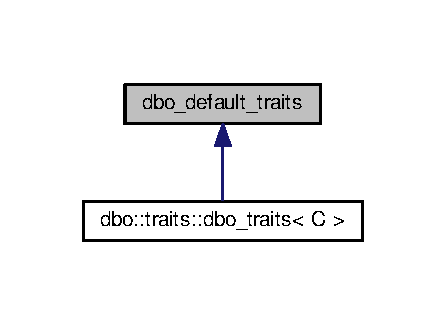
\includegraphics[width=214pt]{structdbo__default__traits__inherit__graph}
\end{center}
\end{figure}
\subsection*{Public Types}
\begin{DoxyCompactItemize}
\item 
typedef long long \hyperlink{structdbo__default__traits_a01f10d78fdf6ae4a23dff88daa60b8ac}{Id\+Type}
\begin{DoxyCompactList}\small\item\em Type of the primary key. \end{DoxyCompactList}\end{DoxyCompactItemize}
\subsection*{Static Public Member Functions}
\begin{DoxyCompactItemize}
\item 
static \hyperlink{structdbo__default__traits_a01f10d78fdf6ae4a23dff88daa60b8ac}{Id\+Type} \hyperlink{structdbo__default__traits_a63d90a044d84c0c5062ebd2b69713484}{invalid\+Id} ()
\begin{DoxyCompactList}\small\item\em Returns the sentinel value for a {\ttfamily null} id. \end{DoxyCompactList}\item 
static boost\+::optional\\*
$<$ std\+::string $>$ \hyperlink{structdbo__default__traits_a7f0ee1558eb51f77cc1843f5fcf19057}{surrogate\+Id\+Field} ()
\begin{DoxyCompactList}\small\item\em Configures the surrogate primary key field. \end{DoxyCompactList}\end{DoxyCompactItemize}


\subsection{Detailed Description}
Default traits for a class mapped with \%Dbo. 

This class provides the default traits. It is convenient (and future proof) to inherit these default traits when customizing the traits for one particular class. 

\subsection{Member Typedef Documentation}
\hypertarget{structdbo__default__traits_a01f10d78fdf6ae4a23dff88daa60b8ac}{\index{dbo\+\_\+default\+\_\+traits@{dbo\+\_\+default\+\_\+traits}!Id\+Type@{Id\+Type}}
\index{Id\+Type@{Id\+Type}!dbo\+\_\+default\+\_\+traits@{dbo\+\_\+default\+\_\+traits}}
\subsubsection[{Id\+Type}]{\setlength{\rightskip}{0pt plus 5cm}typedef long long {\bf dbo\+\_\+default\+\_\+traits\+::\+Id\+Type}}}\label{structdbo__default__traits_a01f10d78fdf6ae4a23dff88daa60b8ac}


Type of the primary key. 

This indicates the type of the primary key, which needs to be {\ttfamily long long} for a surrogate id, but can be any type supported by \hyperlink{namespacedbo_ad1f50f02cb050acf946807959252a93f}{dbo\+::field()} (including composite types) for a natural primary key.

The following operations need to be supported for an id value\+:


\begin{DoxyItemize}
\item {\itshape default constructor}
\item {\itshape copy constructor}
\item serialization to a string (for formatting an error message in exceptions) \+: {\ttfamily std\+::ostream $<$$<$ id}
\item comparison operator (for use as a key in a std\+::map)\+: {\ttfamily id == id}
\item less than operator (for use as a key in a std\+::map)\+: {\ttfamily id $<$ id}
\end{DoxyItemize}

Only the default {\ttfamily long long} is supported for an auto-\/incrementing surrogate primary key. You need to change the default key type typically in conjuction with specifying a natural id, see \hyperlink{namespacedbo_a8d25907296ae8360b3120b7492022c1d}{dbo\+::id()}.

The following example illustrates how to prepare a type to be usable as a composite id type\+:


\begin{DoxyCode}
\textcolor{keyword}{struct }Coordinate \{
  \textcolor{keywordtype}{int} x, y;

  Coordinate()
    : x(-1), y(-1) \{ \}

  \textcolor{keywordtype}{bool} operator== (\textcolor{keyword}{const} Coordinate& other)\textcolor{keyword}{ const }\{
    \textcolor{keywordflow}{return} x == other.x && y == other.y;
  \}

  \textcolor{keywordtype}{bool} operator< (\textcolor{keyword}{const} Coordinate& other)\textcolor{keyword}{ const }\{
    \textcolor{keywordflow}{if} (x < other.x)
      \textcolor{keywordflow}{return} \textcolor{keyword}{true};
    \textcolor{keywordflow}{else} \textcolor{keywordflow}{if} (x == other.x)
      \textcolor{keywordflow}{return} y < other.y;
    \textcolor{keywordflow}{else}
      \textcolor{keywordflow}{return} \textcolor{keyword}{false};
  \}
\};

std::ostream& \hyperlink{namespacedbo_a35fca6f52b51bacd907a2680d534ba1b}{operator<< }(std::ostream& o, \textcolor{keyword}{const} Coordinate& c)
\{
  \textcolor{keywordflow}{return} o << \textcolor{stringliteral}{"("} << c.x << \textcolor{stringliteral}{", "} << c.y << \textcolor{stringliteral}{")"};
\}

  \textcolor{keyword}{namespace }dbo \{

    \textcolor{keyword}{template} <\textcolor{keyword}{class} Action>
    \textcolor{keywordtype}{void} \hyperlink{namespacedbo_ad1f50f02cb050acf946807959252a93f}{field}(Action& action, Coordinate& coordinate, \textcolor{keyword}{const} std::string& name, \textcolor{keywordtype}{int} size = -1)
    \{
      \hyperlink{namespacedbo_ad1f50f02cb050acf946807959252a93f}{field}(action, coordinate.x, name + \textcolor{stringliteral}{"\_x"});
      \hyperlink{namespacedbo_ad1f50f02cb050acf946807959252a93f}{field}(action, coordinate.y, name + \textcolor{stringliteral}{"\_y"});
    \}
  \}
\end{DoxyCode}
 

\subsection{Member Function Documentation}
\hypertarget{structdbo__default__traits_a63d90a044d84c0c5062ebd2b69713484}{\index{dbo\+\_\+default\+\_\+traits@{dbo\+\_\+default\+\_\+traits}!invalid\+Id@{invalid\+Id}}
\index{invalid\+Id@{invalid\+Id}!dbo\+\_\+default\+\_\+traits@{dbo\+\_\+default\+\_\+traits}}
\subsubsection[{invalid\+Id}]{\setlength{\rightskip}{0pt plus 5cm}static {\bf Id\+Type} dbo\+\_\+default\+\_\+traits\+::invalid\+Id (
\begin{DoxyParamCaption}
{}
\end{DoxyParamCaption}
)\hspace{0.3cm}{\ttfamily [inline]}, {\ttfamily [static]}}}\label{structdbo__default__traits_a63d90a044d84c0c5062ebd2b69713484}


Returns the sentinel value for a {\ttfamily null} id. 

When used as a foreign key, this value is used to represent a {\ttfamily null} value.

The default implementation returns -\/1. \hypertarget{structdbo__default__traits_a7f0ee1558eb51f77cc1843f5fcf19057}{\index{dbo\+\_\+default\+\_\+traits@{dbo\+\_\+default\+\_\+traits}!surrogate\+Id\+Field@{surrogate\+Id\+Field}}
\index{surrogate\+Id\+Field@{surrogate\+Id\+Field}!dbo\+\_\+default\+\_\+traits@{dbo\+\_\+default\+\_\+traits}}
\subsubsection[{surrogate\+Id\+Field}]{\setlength{\rightskip}{0pt plus 5cm}static boost\+::optional$<$std\+::string$>$ dbo\+\_\+default\+\_\+traits\+::surrogate\+Id\+Field (
\begin{DoxyParamCaption}
{}
\end{DoxyParamCaption}
)\hspace{0.3cm}{\ttfamily [inline]}, {\ttfamily [static]}}}\label{structdbo__default__traits_a7f0ee1558eb51f77cc1843f5fcf19057}


Configures the surrogate primary key field. 

Returns the field name which is the surrogate primary key, corresponding to the object's id.

You can disable this auto-\/incrementing surrogate id by returning {\ttfamily 0} instead. In that case you will need to define a natural id for your class using \hyperlink{namespacedbo_a8d25907296ae8360b3120b7492022c1d}{dbo\+::id()}.

The default surrogate id database field name is {\ttfamily \char`\"{}id\char`\"{}}. 

The documentation for this class was generated from the following file\+:\begin{DoxyCompactItemize}
\item 
dbo/traits/\hyperlink{dbo__default__traits_8hpp}{dbo\+\_\+default\+\_\+traits.\+hpp}\end{DoxyCompactItemize}

\hypertarget{structdbo_1_1traits_1_1dbo__traits}{\section{dbo\+:\+:traits\+:\+:dbo\+\_\+traits$<$ C $>$ Class Template Reference}
\label{structdbo_1_1traits_1_1dbo__traits}\index{dbo\+::traits\+::dbo\+\_\+traits$<$ C $>$@{dbo\+::traits\+::dbo\+\_\+traits$<$ C $>$}}
}


Traits for a class mapped with \%Dbo.  




{\ttfamily \#include $<$dbo\+\_\+traits.\+hpp$>$}



Inheritance diagram for dbo\+:\+:traits\+:\+:dbo\+\_\+traits$<$ C $>$\+:\nopagebreak
\begin{figure}[H]
\begin{center}
\leavevmode
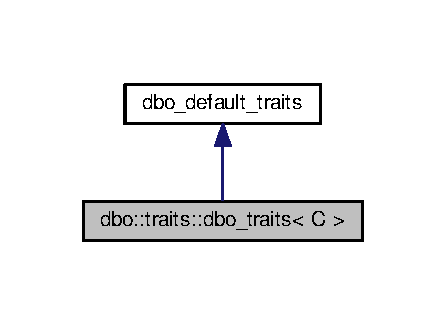
\includegraphics[width=214pt]{structdbo_1_1traits_1_1dbo__traits__inherit__graph}
\end{center}
\end{figure}


Collaboration diagram for dbo\+:\+:traits\+:\+:dbo\+\_\+traits$<$ C $>$\+:\nopagebreak
\begin{figure}[H]
\begin{center}
\leavevmode
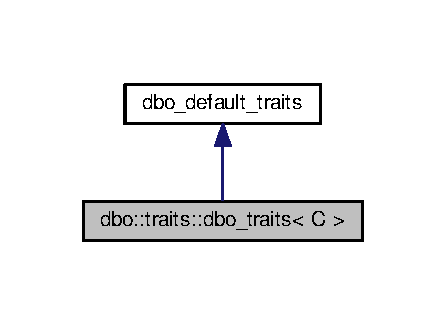
\includegraphics[width=214pt]{structdbo_1_1traits_1_1dbo__traits__coll__graph}
\end{center}
\end{figure}
\subsection*{Additional Inherited Members}


\subsection{Detailed Description}
\subsubsection*{template$<$class C$>$class dbo\+::traits\+::dbo\+\_\+traits$<$ C $>$}

Traits for a class mapped with \%Dbo. 

The traits class provides some of the mapping properties related to the primary key and optimistic concurrency locking using a version field.

See \hyperlink{structdbo__default__traits}{dbo\+\_\+default\+\_\+traits} for default values.

The following example changes the surrogate id field name for a class {\ttfamily Foo} from the default {\ttfamily \char`\"{}id\char`\"{}} to {\ttfamily \char`\"{}foo\+\_\+id\char`\"{}}\+:


\begin{DoxyCode}
\textcolor{keyword}{namespace }dbo \{

  \textcolor{keyword}{template}<>
  \textcolor{keyword}{struct }dbo\_traits<Foo> : \hyperlink{structdbo__default__traits}{dbo\_default\_traits}
  \{
     \textcolor{keyword}{static} \textcolor{keyword}{const} \textcolor{keywordtype}{char} *\hyperlink{structdbo__default__traits_a7f0ee1558eb51f77cc1843f5fcf19057}{surrogateIdField}() \{ \textcolor{keywordflow}{return} \textcolor{stringliteral}{"foo\_id"}; \}
  \};

  \textcolor{comment}{// Necessary if you want to use ptr<const Foo>}
  \textcolor{keyword}{template}<> \textcolor{keyword}{struct }dbo\_traits<const Foo> : dbo\_traits<Foo> \{\};
\}
\end{DoxyCode}


\begin{DoxyNote}{Note}
The safe pattern to define traits is before the class definition, based on a forward declaration. This is necessary since the persist() function relies on this specialization\+: 
\begin{DoxyCode}
\textcolor{keyword}{class }Foo;

  \textcolor{keyword}{namespace }dbo \{
    \textcolor{keyword}{template}<> \textcolor{keyword}{struct }dbo\_traits<Foo> : ... \{ \};
  \}

\textcolor{keyword}{class }Foo \{
  \textcolor{comment}{// definition here, including the persist() function}
\};
\end{DoxyCode}
 
\end{DoxyNote}


The documentation for this class was generated from the following file\+:\begin{DoxyCompactItemize}
\item 
dbo/traits/\hyperlink{dbo__traits_8hpp}{dbo\+\_\+traits.\+hpp}\end{DoxyCompactItemize}

\hypertarget{classdbo_1_1action_1_1_delete}{\section{dbo\+:\+:action\+:\+:Delete$<$ C $>$ Class Template Reference}
\label{classdbo_1_1action_1_1_delete}\index{dbo\+::action\+::\+Delete$<$ C $>$@{dbo\+::action\+::\+Delete$<$ C $>$}}
}


{\ttfamily \#include $<$Delete.\+hpp$>$}

\subsection*{Public Types}
\begin{DoxyCompactItemize}
\item 
using \hyperlink{classdbo_1_1action_1_1_delete_a898e852173a4bace785c9c9d82d7ec43}{Id\+Type} = typename \hyperlink{structdbo_1_1traits_1_1dbo__traits}{traits\+::dbo\+\_\+traits}$<$ C $>$\+::\hyperlink{classdbo_1_1action_1_1_delete_a898e852173a4bace785c9c9d82d7ec43}{Id\+Type}
\end{DoxyCompactItemize}
\subsection*{Public Member Functions}
\begin{DoxyCompactItemize}
\item 
\hyperlink{classdbo_1_1action_1_1_delete_a54b012c688f8a3bcb5e1a7b83b1b0cbb}{Delete} (\hyperlink{classdbo_1_1ptr}{ptr}$<$ C $>$ \hyperlink{classdbo_1_1ptr}{ptr}, std\+::shared\+\_\+ptr$<$ \hyperlink{classdbo_1_1mapping_1_1_mapping}{mapping\+::\+Mapping}$<$ C $>$$>$ mapping, \hyperlink{classdbo_1_1stmt_1_1_prepared_statement}{stmt\+::\+Prepared\+Statement} \&stmt)
\item 
void \hyperlink{classdbo_1_1action_1_1_delete_ad62b6538bec4bf5ca147cb1e167185c5}{visit} ()
\item 
{\footnotesize template$<$typename V $>$ }\\void \hyperlink{classdbo_1_1action_1_1_delete_ad9e186a046fa212f320bb356755d7e9c}{act} (const \hyperlink{classdbo_1_1mapping_1_1_field_ref}{mapping\+::\+Field\+Ref}$<$ V $>$ \&\hyperlink{namespacedbo_ad1f50f02cb050acf946807959252a93f}{field})
\item 
{\footnotesize template$<$typename V $>$ }\\void \hyperlink{classdbo_1_1action_1_1_delete_a8f4fc3e3b29cf499413084b9b022bc4d}{act\+Id} (V \&value, const std\+::string \&name, int size)
\item 
{\footnotesize template$<$class D $>$ }\\void \hyperlink{classdbo_1_1action_1_1_delete_ae28a7db6bd7b2a92fe65b6e3cdb20d11}{act\+Id} (\hyperlink{classdbo_1_1ptr}{ptr}$<$ D $>$ \&value, const std\+::string \&name, int size, int fk\+Constraints)
\item 
{\footnotesize template$<$class D $>$ }\\void \hyperlink{classdbo_1_1action_1_1_delete_ac8d1309f52fb2b7242f4389aabf5d760}{act\+Ptr} (const \hyperlink{classdbo_1_1mapping_1_1_ptr_ref}{mapping\+::\+Ptr\+Ref}$<$ D $>$ \&\hyperlink{namespacedbo_ad1f50f02cb050acf946807959252a93f}{field})
\item 
\hyperlink{classdbo_1_1connection}{connection} \& \hyperlink{classdbo_1_1action_1_1_delete_a224df8996204c37b65f50fa94678ec7a}{conn} ()
\end{DoxyCompactItemize}
\subsection*{Friends}
\begin{DoxyCompactItemize}
\item 
{\footnotesize template$<$class D $>$ }\\class \hyperlink{classdbo_1_1action_1_1_delete_a86bcfdc8a57bb29053c4150ab69352a8}{Delete}
\end{DoxyCompactItemize}


\subsection{Member Typedef Documentation}
\hypertarget{classdbo_1_1action_1_1_delete_a898e852173a4bace785c9c9d82d7ec43}{\index{dbo\+::action\+::\+Delete@{dbo\+::action\+::\+Delete}!Id\+Type@{Id\+Type}}
\index{Id\+Type@{Id\+Type}!dbo\+::action\+::\+Delete@{dbo\+::action\+::\+Delete}}
\subsubsection[{Id\+Type}]{\setlength{\rightskip}{0pt plus 5cm}template$<$class C $>$ using {\bf dbo\+::action\+::\+Delete}$<$ C $>$\+::{\bf Id\+Type} =  typename {\bf traits\+::dbo\+\_\+traits}$<$C$>$\+::{\bf Id\+Type}}}\label{classdbo_1_1action_1_1_delete_a898e852173a4bace785c9c9d82d7ec43}


\subsection{Constructor \& Destructor Documentation}
\hypertarget{classdbo_1_1action_1_1_delete_a54b012c688f8a3bcb5e1a7b83b1b0cbb}{\index{dbo\+::action\+::\+Delete@{dbo\+::action\+::\+Delete}!Delete@{Delete}}
\index{Delete@{Delete}!dbo\+::action\+::\+Delete@{dbo\+::action\+::\+Delete}}
\subsubsection[{Delete}]{\setlength{\rightskip}{0pt plus 5cm}template$<$class C $>$ {\bf dbo\+::action\+::\+Delete}$<$ C $>$\+::{\bf Delete} (
\begin{DoxyParamCaption}
\item[{{\bf ptr}$<$ C $>$}]{ptr, }
\item[{std\+::shared\+\_\+ptr$<$ {\bf mapping\+::\+Mapping}$<$ C $>$$>$}]{mapping, }
\item[{{\bf stmt\+::\+Prepared\+Statement} \&}]{stmt}
\end{DoxyParamCaption}
)}}\label{classdbo_1_1action_1_1_delete_a54b012c688f8a3bcb5e1a7b83b1b0cbb}


\subsection{Member Function Documentation}
\hypertarget{classdbo_1_1action_1_1_delete_ad9e186a046fa212f320bb356755d7e9c}{\index{dbo\+::action\+::\+Delete@{dbo\+::action\+::\+Delete}!act@{act}}
\index{act@{act}!dbo\+::action\+::\+Delete@{dbo\+::action\+::\+Delete}}
\subsubsection[{act}]{\setlength{\rightskip}{0pt plus 5cm}template$<$class C $>$ template$<$typename V $>$ void {\bf dbo\+::action\+::\+Delete}$<$ C $>$\+::act (
\begin{DoxyParamCaption}
\item[{const {\bf mapping\+::\+Field\+Ref}$<$ V $>$ \&}]{field}
\end{DoxyParamCaption}
)}}\label{classdbo_1_1action_1_1_delete_ad9e186a046fa212f320bb356755d7e9c}
\hypertarget{classdbo_1_1action_1_1_delete_a8f4fc3e3b29cf499413084b9b022bc4d}{\index{dbo\+::action\+::\+Delete@{dbo\+::action\+::\+Delete}!act\+Id@{act\+Id}}
\index{act\+Id@{act\+Id}!dbo\+::action\+::\+Delete@{dbo\+::action\+::\+Delete}}
\subsubsection[{act\+Id}]{\setlength{\rightskip}{0pt plus 5cm}template$<$class C $>$ template$<$typename V $>$ void {\bf dbo\+::action\+::\+Delete}$<$ C $>$\+::act\+Id (
\begin{DoxyParamCaption}
\item[{V \&}]{value, }
\item[{const std\+::string \&}]{name, }
\item[{int}]{size}
\end{DoxyParamCaption}
)}}\label{classdbo_1_1action_1_1_delete_a8f4fc3e3b29cf499413084b9b022bc4d}
\hypertarget{classdbo_1_1action_1_1_delete_ae28a7db6bd7b2a92fe65b6e3cdb20d11}{\index{dbo\+::action\+::\+Delete@{dbo\+::action\+::\+Delete}!act\+Id@{act\+Id}}
\index{act\+Id@{act\+Id}!dbo\+::action\+::\+Delete@{dbo\+::action\+::\+Delete}}
\subsubsection[{act\+Id}]{\setlength{\rightskip}{0pt plus 5cm}template$<$class C $>$ template$<$class D $>$ void {\bf dbo\+::action\+::\+Delete}$<$ C $>$\+::act\+Id (
\begin{DoxyParamCaption}
\item[{{\bf ptr}$<$ D $>$ \&}]{value, }
\item[{const std\+::string \&}]{name, }
\item[{int}]{size, }
\item[{int}]{fk\+Constraints}
\end{DoxyParamCaption}
)}}\label{classdbo_1_1action_1_1_delete_ae28a7db6bd7b2a92fe65b6e3cdb20d11}
\hypertarget{classdbo_1_1action_1_1_delete_ac8d1309f52fb2b7242f4389aabf5d760}{\index{dbo\+::action\+::\+Delete@{dbo\+::action\+::\+Delete}!act\+Ptr@{act\+Ptr}}
\index{act\+Ptr@{act\+Ptr}!dbo\+::action\+::\+Delete@{dbo\+::action\+::\+Delete}}
\subsubsection[{act\+Ptr}]{\setlength{\rightskip}{0pt plus 5cm}template$<$class C $>$ template$<$class D $>$ void {\bf dbo\+::action\+::\+Delete}$<$ C $>$\+::act\+Ptr (
\begin{DoxyParamCaption}
\item[{const {\bf mapping\+::\+Ptr\+Ref}$<$ D $>$ \&}]{field}
\end{DoxyParamCaption}
)}}\label{classdbo_1_1action_1_1_delete_ac8d1309f52fb2b7242f4389aabf5d760}
\hypertarget{classdbo_1_1action_1_1_delete_a224df8996204c37b65f50fa94678ec7a}{\index{dbo\+::action\+::\+Delete@{dbo\+::action\+::\+Delete}!conn@{conn}}
\index{conn@{conn}!dbo\+::action\+::\+Delete@{dbo\+::action\+::\+Delete}}
\subsubsection[{conn}]{\setlength{\rightskip}{0pt plus 5cm}template$<$class C $>$ {\bf connection}\& {\bf dbo\+::action\+::\+Delete}$<$ C $>$\+::conn (
\begin{DoxyParamCaption}
{}
\end{DoxyParamCaption}
)\hspace{0.3cm}{\ttfamily [inline]}}}\label{classdbo_1_1action_1_1_delete_a224df8996204c37b65f50fa94678ec7a}
\hypertarget{classdbo_1_1action_1_1_delete_ad62b6538bec4bf5ca147cb1e167185c5}{\index{dbo\+::action\+::\+Delete@{dbo\+::action\+::\+Delete}!visit@{visit}}
\index{visit@{visit}!dbo\+::action\+::\+Delete@{dbo\+::action\+::\+Delete}}
\subsubsection[{visit}]{\setlength{\rightskip}{0pt plus 5cm}template$<$class C $>$ void {\bf dbo\+::action\+::\+Delete}$<$ C $>$\+::visit (
\begin{DoxyParamCaption}
{}
\end{DoxyParamCaption}
)}}\label{classdbo_1_1action_1_1_delete_ad62b6538bec4bf5ca147cb1e167185c5}


\subsection{Friends And Related Function Documentation}
\hypertarget{classdbo_1_1action_1_1_delete_a86bcfdc8a57bb29053c4150ab69352a8}{\index{dbo\+::action\+::\+Delete@{dbo\+::action\+::\+Delete}!Delete@{Delete}}
\index{Delete@{Delete}!dbo\+::action\+::\+Delete@{dbo\+::action\+::\+Delete}}
\subsubsection[{Delete}]{\setlength{\rightskip}{0pt plus 5cm}template$<$class C $>$ template$<$class D $>$ friend class {\bf Delete}\hspace{0.3cm}{\ttfamily [friend]}}}\label{classdbo_1_1action_1_1_delete_a86bcfdc8a57bb29053c4150ab69352a8}


The documentation for this class was generated from the following files\+:\begin{DoxyCompactItemize}
\item 
dbo/action/\hyperlink{_delete_8hpp}{Delete.\+hpp}\item 
dbo/action/\hyperlink{_delete_8cxx}{Delete.\+cxx}\end{DoxyCompactItemize}

\hypertarget{classdbo_1_1_exception}{\section{dbo\+:\+:Exception Class Reference}
\label{classdbo_1_1_exception}\index{dbo\+::\+Exception@{dbo\+::\+Exception}}
}


{\ttfamily \#include $<$Exception.\+h$>$}



Inheritance diagram for dbo\+:\+:Exception\+:\nopagebreak
\begin{figure}[H]
\begin{center}
\leavevmode
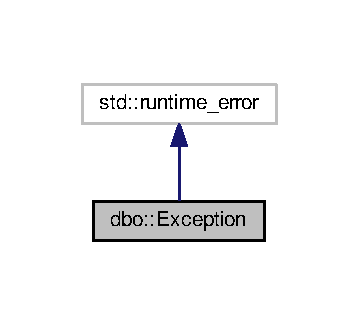
\includegraphics[width=172pt]{classdbo_1_1_exception__inherit__graph}
\end{center}
\end{figure}


Collaboration diagram for dbo\+:\+:Exception\+:\nopagebreak
\begin{figure}[H]
\begin{center}
\leavevmode
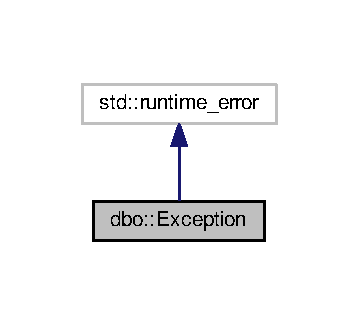
\includegraphics[width=172pt]{classdbo_1_1_exception__coll__graph}
\end{center}
\end{figure}
\subsection*{Public Member Functions}
\begin{DoxyCompactItemize}
\item 
\hyperlink{classdbo_1_1_exception_a52d8037cc4cdcb4fc18651b5669b1621}{Exception} (const std\+::string \&error, const std\+::string \&\hyperlink{classdbo_1_1_exception_aae1affef09ea6691eb7e16ee1cc75edc}{code}=std\+::string())
\item 
virtual \hyperlink{classdbo_1_1_exception_a122aaa1fc274cf2ed943613ae28bb268}{$\sim$\+Exception} ()  throw ()
\item 
std\+::string \hyperlink{classdbo_1_1_exception_aae1affef09ea6691eb7e16ee1cc75edc}{code} () const 
\end{DoxyCompactItemize}


\subsection{Constructor \& Destructor Documentation}
\hypertarget{classdbo_1_1_exception_a52d8037cc4cdcb4fc18651b5669b1621}{\index{dbo\+::\+Exception@{dbo\+::\+Exception}!Exception@{Exception}}
\index{Exception@{Exception}!dbo\+::\+Exception@{dbo\+::\+Exception}}
\subsubsection[{Exception}]{\setlength{\rightskip}{0pt plus 5cm}dbo\+::\+Exception\+::\+Exception (
\begin{DoxyParamCaption}
\item[{const std\+::string \&}]{error, }
\item[{const std\+::string \&}]{code = {\ttfamily std\+:\+:string()}}
\end{DoxyParamCaption}
)\hspace{0.3cm}{\ttfamily [inline]}}}\label{classdbo_1_1_exception_a52d8037cc4cdcb4fc18651b5669b1621}
\hypertarget{classdbo_1_1_exception_a122aaa1fc274cf2ed943613ae28bb268}{\index{dbo\+::\+Exception@{dbo\+::\+Exception}!````~Exception@{$\sim$\+Exception}}
\index{````~Exception@{$\sim$\+Exception}!dbo\+::\+Exception@{dbo\+::\+Exception}}
\subsubsection[{$\sim$\+Exception}]{\setlength{\rightskip}{0pt plus 5cm}virtual dbo\+::\+Exception\+::$\sim$\+Exception (
\begin{DoxyParamCaption}
{}
\end{DoxyParamCaption}
) throw  ) \hspace{0.3cm}{\ttfamily [inline]}, {\ttfamily [virtual]}}}\label{classdbo_1_1_exception_a122aaa1fc274cf2ed943613ae28bb268}


\subsection{Member Function Documentation}
\hypertarget{classdbo_1_1_exception_aae1affef09ea6691eb7e16ee1cc75edc}{\index{dbo\+::\+Exception@{dbo\+::\+Exception}!code@{code}}
\index{code@{code}!dbo\+::\+Exception@{dbo\+::\+Exception}}
\subsubsection[{code}]{\setlength{\rightskip}{0pt plus 5cm}std\+::string dbo\+::\+Exception\+::code (
\begin{DoxyParamCaption}
{}
\end{DoxyParamCaption}
) const\hspace{0.3cm}{\ttfamily [inline]}}}\label{classdbo_1_1_exception_aae1affef09ea6691eb7e16ee1cc75edc}


The documentation for this class was generated from the following file\+:\begin{DoxyCompactItemize}
\item 
dbo/\hyperlink{_exception_8h}{Exception.\+h}\end{DoxyCompactItemize}

\hypertarget{classdbo_1_1mapping_1_1_field_info}{\section{dbo\+:\+:mapping\+:\+:Field\+Info Class Reference}
\label{classdbo_1_1mapping_1_1_field_info}\index{dbo\+::mapping\+::\+Field\+Info@{dbo\+::mapping\+::\+Field\+Info}}
}


Description of a field.  




{\ttfamily \#include $<$Field\+Info.\+h$>$}

\subsection*{Public Types}
\begin{DoxyCompactItemize}
\item 
enum \hyperlink{classdbo_1_1mapping_1_1_field_info_ace9623c079f46b2c932e339e68c001dd}{Flags} \{ \\*
\hyperlink{classdbo_1_1mapping_1_1_field_info_ace9623c079f46b2c932e339e68c001dda6de7a4ea4dae9a1d3ee99bdfe62ea265}{Surrogate\+Id} = 0x1, 
\hyperlink{classdbo_1_1mapping_1_1_field_info_ace9623c079f46b2c932e339e68c001ddadf26125864257adc9fd3814a3ea24582}{Natural\+Id} = 0x2, 
\hyperlink{classdbo_1_1mapping_1_1_field_info_ace9623c079f46b2c932e339e68c001ddab3033d795a06974f753a927b829b237c}{Mutable} = 0x8, 
\hyperlink{classdbo_1_1mapping_1_1_field_info_ace9623c079f46b2c932e339e68c001dda488d560d149ccf2cbc43042da063f80d}{Needs\+Quotes} = 0x10, 
\\*
\hyperlink{classdbo_1_1mapping_1_1_field_info_ace9623c079f46b2c932e339e68c001dda07e0b2f157b634fe26a5c916182ec1b3}{Foreign\+Key} = 0x20, 
\hyperlink{classdbo_1_1mapping_1_1_field_info_ace9623c079f46b2c932e339e68c001dda432cc6112f7921b2211e8ddc78c73b8d}{First\+Dbo\+Field} = 0x40
 \}
\begin{DoxyCompactList}\small\item\em Flags. \end{DoxyCompactList}\end{DoxyCompactItemize}
\subsection*{Public Member Functions}
\begin{DoxyCompactItemize}
\item 
\hyperlink{classdbo_1_1mapping_1_1_field_info_a8763d05cee7a73c3b60cb133467c65b2}{Field\+Info} (const std\+::string \&\hyperlink{classdbo_1_1mapping_1_1_field_info_aa684340deb7dabfb5eab22c4589c7476}{name}, const std\+::type\+\_\+info $\ast$\hyperlink{classdbo_1_1mapping_1_1_field_info_a4321bb42c7c9d8296db5180b94a736f6}{type}, const std\+::string \&\hyperlink{classdbo_1_1mapping_1_1_field_info_a29f7e7f762345f1915033a9a456cd5d0}{sql\+Type}, int flags)
\begin{DoxyCompactList}\small\item\em Creates a field description. \end{DoxyCompactList}\item 
\hyperlink{classdbo_1_1mapping_1_1_field_info_acca8ec52e6b2d6f1810d499b30dd1aaa}{Field\+Info} (const std\+::string \&\hyperlink{classdbo_1_1mapping_1_1_field_info_aa684340deb7dabfb5eab22c4589c7476}{name}, const std\+::type\+\_\+info $\ast$\hyperlink{classdbo_1_1mapping_1_1_field_info_a4321bb42c7c9d8296db5180b94a736f6}{type}, const std\+::string \&\hyperlink{classdbo_1_1mapping_1_1_field_info_a29f7e7f762345f1915033a9a456cd5d0}{sql\+Type}, const std\+::string \&\hyperlink{classdbo_1_1mapping_1_1_field_info_ac90a4d26a0c091ba0a93960a8d8a8464}{foreign\+Key\+Table}, const std\+::string \&\hyperlink{classdbo_1_1mapping_1_1_field_info_adbc55f9c113054bed81ed7dd22aca09a}{foreign\+Key\+Name}, int flags, int \hyperlink{classdbo_1_1mapping_1_1_field_info_ae7700af51bf1672d8d2db4a52b885c4d}{fk\+Constraints})
\begin{DoxyCompactList}\small\item\em Creates a field description. \end{DoxyCompactList}\item 
void \hyperlink{classdbo_1_1mapping_1_1_field_info_adc3ba59211a120f92f09bfefa43a65b0}{set\+Qualifier} (const std\+::string \&\hyperlink{classdbo_1_1mapping_1_1_field_info_a3891d63e2efd86128fd6f6ae10979b22}{qualifier}, bool first\+Qualified=false)
\begin{DoxyCompactList}\small\item\em Sets a qualifier for the field. \end{DoxyCompactList}\item 
const std\+::string \& \hyperlink{classdbo_1_1mapping_1_1_field_info_aa684340deb7dabfb5eab22c4589c7476}{name} () const 
\begin{DoxyCompactList}\small\item\em Returns the field name. \end{DoxyCompactList}\item 
const std\+::string \& \hyperlink{classdbo_1_1mapping_1_1_field_info_a29f7e7f762345f1915033a9a456cd5d0}{sql\+Type} () const 
\begin{DoxyCompactList}\small\item\em Returns the field S\+Q\+L type. \end{DoxyCompactList}\item 
const std\+::string \& \hyperlink{classdbo_1_1mapping_1_1_field_info_a3891d63e2efd86128fd6f6ae10979b22}{qualifier} () const 
\begin{DoxyCompactList}\small\item\em Returns the field qualifier. \end{DoxyCompactList}\item 
const std\+::type\+\_\+info $\ast$ \hyperlink{classdbo_1_1mapping_1_1_field_info_a4321bb42c7c9d8296db5180b94a736f6}{type} () const 
\begin{DoxyCompactList}\small\item\em Returns the field type. \end{DoxyCompactList}\item 
bool \hyperlink{classdbo_1_1mapping_1_1_field_info_a1dce2395f113563a2525d7e1d150245d}{is\+Id\+Field} () const 
\begin{DoxyCompactList}\small\item\em Returns whether the field is an Id field. \end{DoxyCompactList}\item 
bool \hyperlink{classdbo_1_1mapping_1_1_field_info_a37ca3f6a5116fcc0afe4ea113dafe07a}{is\+Natural\+Id\+Field} () const 
\begin{DoxyCompactList}\small\item\em Returns whether the field is a Natural Id field. \end{DoxyCompactList}\item 
bool \hyperlink{classdbo_1_1mapping_1_1_field_info_a985286424bae56da1b84d3d1c1dcd128}{is\+Surrogate\+Id\+Field} () const 
\begin{DoxyCompactList}\small\item\em Returns whether the field is a Surroaget Id field. \end{DoxyCompactList}\item 
bool \hyperlink{classdbo_1_1mapping_1_1_field_info_aba30a705ddc3779e976ad2014fc19fbf}{is\+Mutable} () const 
\begin{DoxyCompactList}\small\item\em Returns whether the field is mutable. \end{DoxyCompactList}\item 
bool \hyperlink{classdbo_1_1mapping_1_1_field_info_abba9be734bfea0b4cf9c4408dcaa6d6e}{needs\+Quotes} () const 
\begin{DoxyCompactList}\small\item\em Returns whether the field name needs to be quoted. \end{DoxyCompactList}\item 
bool \hyperlink{classdbo_1_1mapping_1_1_field_info_ac56bc147c4c4385ae1b14e97055592a0}{is\+Foreign\+Key} () const 
\begin{DoxyCompactList}\small\item\em Returns whether the field is part of a foreign key. \end{DoxyCompactList}\item 
bool \hyperlink{classdbo_1_1mapping_1_1_field_info_ae694e49e7041d3a2795c87a7e2fa5064}{is\+First\+Dbo\+Field} () const 
\item 
std\+::string \hyperlink{classdbo_1_1mapping_1_1_field_info_adbc55f9c113054bed81ed7dd22aca09a}{foreign\+Key\+Name} () const 
\item 
std\+::string \hyperlink{classdbo_1_1mapping_1_1_field_info_ac90a4d26a0c091ba0a93960a8d8a8464}{foreign\+Key\+Table} () const 
\item 
int \hyperlink{classdbo_1_1mapping_1_1_field_info_ae7700af51bf1672d8d2db4a52b885c4d}{fk\+Constraints} () const 
\item 
std\+::string \hyperlink{classdbo_1_1mapping_1_1_field_info_a73d24bf3d349158bb842452a00c8655c}{sql} () const 
\item 
std\+::string \hyperlink{classdbo_1_1mapping_1_1_field_info_aafa055b3aa50d4a02cda73cb545d0a91}{debug} (int tab)
\end{DoxyCompactItemize}


\subsection{Detailed Description}
Description of a field. 

\begin{DoxySeeAlso}{See also}
query\+\_\+result\+\_\+traits\+::get\+Fields(), Query\+::fields() 
\end{DoxySeeAlso}


\subsection{Member Enumeration Documentation}
\hypertarget{classdbo_1_1mapping_1_1_field_info_ace9623c079f46b2c932e339e68c001dd}{\index{dbo\+::mapping\+::\+Field\+Info@{dbo\+::mapping\+::\+Field\+Info}!Flags@{Flags}}
\index{Flags@{Flags}!dbo\+::mapping\+::\+Field\+Info@{dbo\+::mapping\+::\+Field\+Info}}
\subsubsection[{Flags}]{\setlength{\rightskip}{0pt plus 5cm}enum {\bf dbo\+::mapping\+::\+Field\+Info\+::\+Flags}}}\label{classdbo_1_1mapping_1_1_field_info_ace9623c079f46b2c932e339e68c001dd}


Flags. 

\begin{Desc}
\item[Enumerator]\par
\begin{description}
\index{Surrogate\+Id@{Surrogate\+Id}!dbo\+::mapping\+::\+Field\+Info@{dbo\+::mapping\+::\+Field\+Info}}\index{dbo\+::mapping\+::\+Field\+Info@{dbo\+::mapping\+::\+Field\+Info}!Surrogate\+Id@{Surrogate\+Id}}\item[{\em 
\hypertarget{classdbo_1_1mapping_1_1_field_info_ace9623c079f46b2c932e339e68c001dda6de7a4ea4dae9a1d3ee99bdfe62ea265}{Surrogate\+Id}\label{classdbo_1_1mapping_1_1_field_info_ace9623c079f46b2c932e339e68c001dda6de7a4ea4dae9a1d3ee99bdfe62ea265}
}]Field is a surrogate id. \index{Natural\+Id@{Natural\+Id}!dbo\+::mapping\+::\+Field\+Info@{dbo\+::mapping\+::\+Field\+Info}}\index{dbo\+::mapping\+::\+Field\+Info@{dbo\+::mapping\+::\+Field\+Info}!Natural\+Id@{Natural\+Id}}\item[{\em 
\hypertarget{classdbo_1_1mapping_1_1_field_info_ace9623c079f46b2c932e339e68c001ddadf26125864257adc9fd3814a3ea24582}{Natural\+Id}\label{classdbo_1_1mapping_1_1_field_info_ace9623c079f46b2c932e339e68c001ddadf26125864257adc9fd3814a3ea24582}
}]Field is (part of) a natural id. \index{Mutable@{Mutable}!dbo\+::mapping\+::\+Field\+Info@{dbo\+::mapping\+::\+Field\+Info}}\index{dbo\+::mapping\+::\+Field\+Info@{dbo\+::mapping\+::\+Field\+Info}!Mutable@{Mutable}}\item[{\em 
\hypertarget{classdbo_1_1mapping_1_1_field_info_ace9623c079f46b2c932e339e68c001ddab3033d795a06974f753a927b829b237c}{Mutable}\label{classdbo_1_1mapping_1_1_field_info_ace9623c079f46b2c932e339e68c001ddab3033d795a06974f753a927b829b237c}
}]Field can be edited. \index{Needs\+Quotes@{Needs\+Quotes}!dbo\+::mapping\+::\+Field\+Info@{dbo\+::mapping\+::\+Field\+Info}}\index{dbo\+::mapping\+::\+Field\+Info@{dbo\+::mapping\+::\+Field\+Info}!Needs\+Quotes@{Needs\+Quotes}}\item[{\em 
\hypertarget{classdbo_1_1mapping_1_1_field_info_ace9623c079f46b2c932e339e68c001dda488d560d149ccf2cbc43042da063f80d}{Needs\+Quotes}\label{classdbo_1_1mapping_1_1_field_info_ace9623c079f46b2c932e339e68c001dda488d560d149ccf2cbc43042da063f80d}
}]Field name needs quotes when using in S\+Q\+L. \index{Foreign\+Key@{Foreign\+Key}!dbo\+::mapping\+::\+Field\+Info@{dbo\+::mapping\+::\+Field\+Info}}\index{dbo\+::mapping\+::\+Field\+Info@{dbo\+::mapping\+::\+Field\+Info}!Foreign\+Key@{Foreign\+Key}}\item[{\em 
\hypertarget{classdbo_1_1mapping_1_1_field_info_ace9623c079f46b2c932e339e68c001dda07e0b2f157b634fe26a5c916182ec1b3}{Foreign\+Key}\label{classdbo_1_1mapping_1_1_field_info_ace9623c079f46b2c932e339e68c001dda07e0b2f157b634fe26a5c916182ec1b3}
}]Field is (part of) a foreign key. \index{First\+Dbo\+Field@{First\+Dbo\+Field}!dbo\+::mapping\+::\+Field\+Info@{dbo\+::mapping\+::\+Field\+Info}}\index{dbo\+::mapping\+::\+Field\+Info@{dbo\+::mapping\+::\+Field\+Info}!First\+Dbo\+Field@{First\+Dbo\+Field}}\item[{\em 
\hypertarget{classdbo_1_1mapping_1_1_field_info_ace9623c079f46b2c932e339e68c001dda432cc6112f7921b2211e8ddc78c73b8d}{First\+Dbo\+Field}\label{classdbo_1_1mapping_1_1_field_info_ace9623c079f46b2c932e339e68c001dda432cc6112f7921b2211e8ddc78c73b8d}
}]\end{description}
\end{Desc}


\subsection{Constructor \& Destructor Documentation}
\hypertarget{classdbo_1_1mapping_1_1_field_info_a8763d05cee7a73c3b60cb133467c65b2}{\index{dbo\+::mapping\+::\+Field\+Info@{dbo\+::mapping\+::\+Field\+Info}!Field\+Info@{Field\+Info}}
\index{Field\+Info@{Field\+Info}!dbo\+::mapping\+::\+Field\+Info@{dbo\+::mapping\+::\+Field\+Info}}
\subsubsection[{Field\+Info}]{\setlength{\rightskip}{0pt plus 5cm}Field\+Info\+::\+Field\+Info (
\begin{DoxyParamCaption}
\item[{const std\+::string \&}]{name, }
\item[{const std\+::type\+\_\+info $\ast$}]{type, }
\item[{const std\+::string \&}]{sql\+Type, }
\item[{int}]{flags}
\end{DoxyParamCaption}
)}}\label{classdbo_1_1mapping_1_1_field_info_a8763d05cee7a73c3b60cb133467c65b2}


Creates a field description. 

\hypertarget{classdbo_1_1mapping_1_1_field_info_acca8ec52e6b2d6f1810d499b30dd1aaa}{\index{dbo\+::mapping\+::\+Field\+Info@{dbo\+::mapping\+::\+Field\+Info}!Field\+Info@{Field\+Info}}
\index{Field\+Info@{Field\+Info}!dbo\+::mapping\+::\+Field\+Info@{dbo\+::mapping\+::\+Field\+Info}}
\subsubsection[{Field\+Info}]{\setlength{\rightskip}{0pt plus 5cm}Field\+Info\+::\+Field\+Info (
\begin{DoxyParamCaption}
\item[{const std\+::string \&}]{name, }
\item[{const std\+::type\+\_\+info $\ast$}]{type, }
\item[{const std\+::string \&}]{sql\+Type, }
\item[{const std\+::string \&}]{foreign\+Key\+Table, }
\item[{const std\+::string \&}]{foreign\+Key\+Name, }
\item[{int}]{flags, }
\item[{int}]{fk\+Constraints}
\end{DoxyParamCaption}
)}}\label{classdbo_1_1mapping_1_1_field_info_acca8ec52e6b2d6f1810d499b30dd1aaa}


Creates a field description. 



\subsection{Member Function Documentation}
\hypertarget{classdbo_1_1mapping_1_1_field_info_aafa055b3aa50d4a02cda73cb545d0a91}{\index{dbo\+::mapping\+::\+Field\+Info@{dbo\+::mapping\+::\+Field\+Info}!debug@{debug}}
\index{debug@{debug}!dbo\+::mapping\+::\+Field\+Info@{dbo\+::mapping\+::\+Field\+Info}}
\subsubsection[{debug}]{\setlength{\rightskip}{0pt plus 5cm}std\+::string Field\+Info\+::debug (
\begin{DoxyParamCaption}
\item[{int}]{tab}
\end{DoxyParamCaption}
)}}\label{classdbo_1_1mapping_1_1_field_info_aafa055b3aa50d4a02cda73cb545d0a91}
\hypertarget{classdbo_1_1mapping_1_1_field_info_ae7700af51bf1672d8d2db4a52b885c4d}{\index{dbo\+::mapping\+::\+Field\+Info@{dbo\+::mapping\+::\+Field\+Info}!fk\+Constraints@{fk\+Constraints}}
\index{fk\+Constraints@{fk\+Constraints}!dbo\+::mapping\+::\+Field\+Info@{dbo\+::mapping\+::\+Field\+Info}}
\subsubsection[{fk\+Constraints}]{\setlength{\rightskip}{0pt plus 5cm}int dbo\+::mapping\+::\+Field\+Info\+::fk\+Constraints (
\begin{DoxyParamCaption}
{}
\end{DoxyParamCaption}
) const\hspace{0.3cm}{\ttfamily [inline]}}}\label{classdbo_1_1mapping_1_1_field_info_ae7700af51bf1672d8d2db4a52b885c4d}
\hypertarget{classdbo_1_1mapping_1_1_field_info_adbc55f9c113054bed81ed7dd22aca09a}{\index{dbo\+::mapping\+::\+Field\+Info@{dbo\+::mapping\+::\+Field\+Info}!foreign\+Key\+Name@{foreign\+Key\+Name}}
\index{foreign\+Key\+Name@{foreign\+Key\+Name}!dbo\+::mapping\+::\+Field\+Info@{dbo\+::mapping\+::\+Field\+Info}}
\subsubsection[{foreign\+Key\+Name}]{\setlength{\rightskip}{0pt plus 5cm}std\+::string dbo\+::mapping\+::\+Field\+Info\+::foreign\+Key\+Name (
\begin{DoxyParamCaption}
{}
\end{DoxyParamCaption}
) const\hspace{0.3cm}{\ttfamily [inline]}}}\label{classdbo_1_1mapping_1_1_field_info_adbc55f9c113054bed81ed7dd22aca09a}
\hypertarget{classdbo_1_1mapping_1_1_field_info_ac90a4d26a0c091ba0a93960a8d8a8464}{\index{dbo\+::mapping\+::\+Field\+Info@{dbo\+::mapping\+::\+Field\+Info}!foreign\+Key\+Table@{foreign\+Key\+Table}}
\index{foreign\+Key\+Table@{foreign\+Key\+Table}!dbo\+::mapping\+::\+Field\+Info@{dbo\+::mapping\+::\+Field\+Info}}
\subsubsection[{foreign\+Key\+Table}]{\setlength{\rightskip}{0pt plus 5cm}std\+::string dbo\+::mapping\+::\+Field\+Info\+::foreign\+Key\+Table (
\begin{DoxyParamCaption}
{}
\end{DoxyParamCaption}
) const\hspace{0.3cm}{\ttfamily [inline]}}}\label{classdbo_1_1mapping_1_1_field_info_ac90a4d26a0c091ba0a93960a8d8a8464}
\hypertarget{classdbo_1_1mapping_1_1_field_info_ae694e49e7041d3a2795c87a7e2fa5064}{\index{dbo\+::mapping\+::\+Field\+Info@{dbo\+::mapping\+::\+Field\+Info}!is\+First\+Dbo\+Field@{is\+First\+Dbo\+Field}}
\index{is\+First\+Dbo\+Field@{is\+First\+Dbo\+Field}!dbo\+::mapping\+::\+Field\+Info@{dbo\+::mapping\+::\+Field\+Info}}
\subsubsection[{is\+First\+Dbo\+Field}]{\setlength{\rightskip}{0pt plus 5cm}bool dbo\+::mapping\+::\+Field\+Info\+::is\+First\+Dbo\+Field (
\begin{DoxyParamCaption}
{}
\end{DoxyParamCaption}
) const\hspace{0.3cm}{\ttfamily [inline]}}}\label{classdbo_1_1mapping_1_1_field_info_ae694e49e7041d3a2795c87a7e2fa5064}
\hypertarget{classdbo_1_1mapping_1_1_field_info_ac56bc147c4c4385ae1b14e97055592a0}{\index{dbo\+::mapping\+::\+Field\+Info@{dbo\+::mapping\+::\+Field\+Info}!is\+Foreign\+Key@{is\+Foreign\+Key}}
\index{is\+Foreign\+Key@{is\+Foreign\+Key}!dbo\+::mapping\+::\+Field\+Info@{dbo\+::mapping\+::\+Field\+Info}}
\subsubsection[{is\+Foreign\+Key}]{\setlength{\rightskip}{0pt plus 5cm}bool dbo\+::mapping\+::\+Field\+Info\+::is\+Foreign\+Key (
\begin{DoxyParamCaption}
{}
\end{DoxyParamCaption}
) const\hspace{0.3cm}{\ttfamily [inline]}}}\label{classdbo_1_1mapping_1_1_field_info_ac56bc147c4c4385ae1b14e97055592a0}


Returns whether the field is part of a foreign key. 

\hypertarget{classdbo_1_1mapping_1_1_field_info_a1dce2395f113563a2525d7e1d150245d}{\index{dbo\+::mapping\+::\+Field\+Info@{dbo\+::mapping\+::\+Field\+Info}!is\+Id\+Field@{is\+Id\+Field}}
\index{is\+Id\+Field@{is\+Id\+Field}!dbo\+::mapping\+::\+Field\+Info@{dbo\+::mapping\+::\+Field\+Info}}
\subsubsection[{is\+Id\+Field}]{\setlength{\rightskip}{0pt plus 5cm}bool dbo\+::mapping\+::\+Field\+Info\+::is\+Id\+Field (
\begin{DoxyParamCaption}
{}
\end{DoxyParamCaption}
) const\hspace{0.3cm}{\ttfamily [inline]}}}\label{classdbo_1_1mapping_1_1_field_info_a1dce2395f113563a2525d7e1d150245d}


Returns whether the field is an Id field. 

\hypertarget{classdbo_1_1mapping_1_1_field_info_aba30a705ddc3779e976ad2014fc19fbf}{\index{dbo\+::mapping\+::\+Field\+Info@{dbo\+::mapping\+::\+Field\+Info}!is\+Mutable@{is\+Mutable}}
\index{is\+Mutable@{is\+Mutable}!dbo\+::mapping\+::\+Field\+Info@{dbo\+::mapping\+::\+Field\+Info}}
\subsubsection[{is\+Mutable}]{\setlength{\rightskip}{0pt plus 5cm}bool dbo\+::mapping\+::\+Field\+Info\+::is\+Mutable (
\begin{DoxyParamCaption}
{}
\end{DoxyParamCaption}
) const\hspace{0.3cm}{\ttfamily [inline]}}}\label{classdbo_1_1mapping_1_1_field_info_aba30a705ddc3779e976ad2014fc19fbf}


Returns whether the field is mutable. 

\hypertarget{classdbo_1_1mapping_1_1_field_info_a37ca3f6a5116fcc0afe4ea113dafe07a}{\index{dbo\+::mapping\+::\+Field\+Info@{dbo\+::mapping\+::\+Field\+Info}!is\+Natural\+Id\+Field@{is\+Natural\+Id\+Field}}
\index{is\+Natural\+Id\+Field@{is\+Natural\+Id\+Field}!dbo\+::mapping\+::\+Field\+Info@{dbo\+::mapping\+::\+Field\+Info}}
\subsubsection[{is\+Natural\+Id\+Field}]{\setlength{\rightskip}{0pt plus 5cm}bool dbo\+::mapping\+::\+Field\+Info\+::is\+Natural\+Id\+Field (
\begin{DoxyParamCaption}
{}
\end{DoxyParamCaption}
) const\hspace{0.3cm}{\ttfamily [inline]}}}\label{classdbo_1_1mapping_1_1_field_info_a37ca3f6a5116fcc0afe4ea113dafe07a}


Returns whether the field is a Natural Id field. 

\hypertarget{classdbo_1_1mapping_1_1_field_info_a985286424bae56da1b84d3d1c1dcd128}{\index{dbo\+::mapping\+::\+Field\+Info@{dbo\+::mapping\+::\+Field\+Info}!is\+Surrogate\+Id\+Field@{is\+Surrogate\+Id\+Field}}
\index{is\+Surrogate\+Id\+Field@{is\+Surrogate\+Id\+Field}!dbo\+::mapping\+::\+Field\+Info@{dbo\+::mapping\+::\+Field\+Info}}
\subsubsection[{is\+Surrogate\+Id\+Field}]{\setlength{\rightskip}{0pt plus 5cm}bool dbo\+::mapping\+::\+Field\+Info\+::is\+Surrogate\+Id\+Field (
\begin{DoxyParamCaption}
{}
\end{DoxyParamCaption}
) const\hspace{0.3cm}{\ttfamily [inline]}}}\label{classdbo_1_1mapping_1_1_field_info_a985286424bae56da1b84d3d1c1dcd128}


Returns whether the field is a Surroaget Id field. 

\hypertarget{classdbo_1_1mapping_1_1_field_info_aa684340deb7dabfb5eab22c4589c7476}{\index{dbo\+::mapping\+::\+Field\+Info@{dbo\+::mapping\+::\+Field\+Info}!name@{name}}
\index{name@{name}!dbo\+::mapping\+::\+Field\+Info@{dbo\+::mapping\+::\+Field\+Info}}
\subsubsection[{name}]{\setlength{\rightskip}{0pt plus 5cm}const std\+::string\& dbo\+::mapping\+::\+Field\+Info\+::name (
\begin{DoxyParamCaption}
{}
\end{DoxyParamCaption}
) const\hspace{0.3cm}{\ttfamily [inline]}}}\label{classdbo_1_1mapping_1_1_field_info_aa684340deb7dabfb5eab22c4589c7476}


Returns the field name. 

\hypertarget{classdbo_1_1mapping_1_1_field_info_abba9be734bfea0b4cf9c4408dcaa6d6e}{\index{dbo\+::mapping\+::\+Field\+Info@{dbo\+::mapping\+::\+Field\+Info}!needs\+Quotes@{needs\+Quotes}}
\index{needs\+Quotes@{needs\+Quotes}!dbo\+::mapping\+::\+Field\+Info@{dbo\+::mapping\+::\+Field\+Info}}
\subsubsection[{needs\+Quotes}]{\setlength{\rightskip}{0pt plus 5cm}bool dbo\+::mapping\+::\+Field\+Info\+::needs\+Quotes (
\begin{DoxyParamCaption}
{}
\end{DoxyParamCaption}
) const\hspace{0.3cm}{\ttfamily [inline]}}}\label{classdbo_1_1mapping_1_1_field_info_abba9be734bfea0b4cf9c4408dcaa6d6e}


Returns whether the field name needs to be quoted. 

\hypertarget{classdbo_1_1mapping_1_1_field_info_a3891d63e2efd86128fd6f6ae10979b22}{\index{dbo\+::mapping\+::\+Field\+Info@{dbo\+::mapping\+::\+Field\+Info}!qualifier@{qualifier}}
\index{qualifier@{qualifier}!dbo\+::mapping\+::\+Field\+Info@{dbo\+::mapping\+::\+Field\+Info}}
\subsubsection[{qualifier}]{\setlength{\rightskip}{0pt plus 5cm}const std\+::string\& dbo\+::mapping\+::\+Field\+Info\+::qualifier (
\begin{DoxyParamCaption}
{}
\end{DoxyParamCaption}
) const\hspace{0.3cm}{\ttfamily [inline]}}}\label{classdbo_1_1mapping_1_1_field_info_a3891d63e2efd86128fd6f6ae10979b22}


Returns the field qualifier. 

\hypertarget{classdbo_1_1mapping_1_1_field_info_adc3ba59211a120f92f09bfefa43a65b0}{\index{dbo\+::mapping\+::\+Field\+Info@{dbo\+::mapping\+::\+Field\+Info}!set\+Qualifier@{set\+Qualifier}}
\index{set\+Qualifier@{set\+Qualifier}!dbo\+::mapping\+::\+Field\+Info@{dbo\+::mapping\+::\+Field\+Info}}
\subsubsection[{set\+Qualifier}]{\setlength{\rightskip}{0pt plus 5cm}void dbo\+::mapping\+::\+Field\+Info\+::set\+Qualifier (
\begin{DoxyParamCaption}
\item[{const std\+::string \&}]{qualifier, }
\item[{bool}]{first\+Qualified = {\ttfamily false}}
\end{DoxyParamCaption}
)}}\label{classdbo_1_1mapping_1_1_field_info_adc3ba59211a120f92f09bfefa43a65b0}


Sets a qualifier for the field. 

\hypertarget{classdbo_1_1mapping_1_1_field_info_a73d24bf3d349158bb842452a00c8655c}{\index{dbo\+::mapping\+::\+Field\+Info@{dbo\+::mapping\+::\+Field\+Info}!sql@{sql}}
\index{sql@{sql}!dbo\+::mapping\+::\+Field\+Info@{dbo\+::mapping\+::\+Field\+Info}}
\subsubsection[{sql}]{\setlength{\rightskip}{0pt plus 5cm}std\+::string dbo\+::mapping\+::\+Field\+Info\+::sql (
\begin{DoxyParamCaption}
{}
\end{DoxyParamCaption}
) const}}\label{classdbo_1_1mapping_1_1_field_info_a73d24bf3d349158bb842452a00c8655c}
\hypertarget{classdbo_1_1mapping_1_1_field_info_a29f7e7f762345f1915033a9a456cd5d0}{\index{dbo\+::mapping\+::\+Field\+Info@{dbo\+::mapping\+::\+Field\+Info}!sql\+Type@{sql\+Type}}
\index{sql\+Type@{sql\+Type}!dbo\+::mapping\+::\+Field\+Info@{dbo\+::mapping\+::\+Field\+Info}}
\subsubsection[{sql\+Type}]{\setlength{\rightskip}{0pt plus 5cm}const std\+::string\& dbo\+::mapping\+::\+Field\+Info\+::sql\+Type (
\begin{DoxyParamCaption}
{}
\end{DoxyParamCaption}
) const\hspace{0.3cm}{\ttfamily [inline]}}}\label{classdbo_1_1mapping_1_1_field_info_a29f7e7f762345f1915033a9a456cd5d0}


Returns the field S\+Q\+L type. 

\hypertarget{classdbo_1_1mapping_1_1_field_info_a4321bb42c7c9d8296db5180b94a736f6}{\index{dbo\+::mapping\+::\+Field\+Info@{dbo\+::mapping\+::\+Field\+Info}!type@{type}}
\index{type@{type}!dbo\+::mapping\+::\+Field\+Info@{dbo\+::mapping\+::\+Field\+Info}}
\subsubsection[{type}]{\setlength{\rightskip}{0pt plus 5cm}const std\+::type\+\_\+info$\ast$ dbo\+::mapping\+::\+Field\+Info\+::type (
\begin{DoxyParamCaption}
{}
\end{DoxyParamCaption}
) const\hspace{0.3cm}{\ttfamily [inline]}}}\label{classdbo_1_1mapping_1_1_field_info_a4321bb42c7c9d8296db5180b94a736f6}


Returns the field type. 



The documentation for this class was generated from the following files\+:\begin{DoxyCompactItemize}
\item 
dbo/mapping/\hyperlink{_field_info_8h}{Field\+Info.\+h}\item 
dbo/mapping/\hyperlink{_field_info_8cpp}{Field\+Info.\+cpp}\end{DoxyCompactItemize}

\hypertarget{classdbo_1_1mapping_1_1_field_ref}{\section{dbo\+:\+:mapping\+:\+:Field\+Ref$<$ T $>$ Class Template Reference}
\label{classdbo_1_1mapping_1_1_field_ref}\index{dbo\+::mapping\+::\+Field\+Ref$<$ T $>$@{dbo\+::mapping\+::\+Field\+Ref$<$ T $>$}}
}


{\ttfamily \#include $<$Bulk\+Insert.\+hpp$>$}

\subsection*{Public Member Functions}
\begin{DoxyCompactItemize}
\item 
\hyperlink{classdbo_1_1mapping_1_1_field_ref_a6e90b688f02b8d7de0c5e6fbfbcf897c}{Field\+Ref} (V \&\hyperlink{classdbo_1_1mapping_1_1_field_ref_ad53542241b5f5e9f4055051f00ee7815}{value}, const std\+::string \&\hyperlink{classdbo_1_1mapping_1_1_field_ref_a6a5dbebdfd48f16fe8290ad8f0f304d3}{name}, int \hyperlink{classdbo_1_1mapping_1_1_field_ref_a84a3a0032b7dea68c65b5d66a6cb016f}{size})
\item 
const std\+::string \& \hyperlink{classdbo_1_1mapping_1_1_field_ref_a6a5dbebdfd48f16fe8290ad8f0f304d3}{name} () const 
\item 
int \hyperlink{classdbo_1_1mapping_1_1_field_ref_a84a3a0032b7dea68c65b5d66a6cb016f}{size} () const 
\item 
std\+::string \hyperlink{classdbo_1_1mapping_1_1_field_ref_af74da16080f2a33e08d4a4d8f46c06da}{sql\+Type} () const 
\item 
const std\+::type\+\_\+info $\ast$ \hyperlink{classdbo_1_1mapping_1_1_field_ref_a0a232586ede5bae838f6dafe14d771de}{type} () const 
\item 
V \& \hyperlink{classdbo_1_1mapping_1_1_field_ref_ad53542241b5f5e9f4055051f00ee7815}{value} () const 
\item 
void \hyperlink{classdbo_1_1mapping_1_1_field_ref_ae2736819ccc79e1cb054f1a58acde56d}{set\+Value} (const V \&\hyperlink{classdbo_1_1mapping_1_1_field_ref_ad53542241b5f5e9f4055051f00ee7815}{value}) const 
\end{DoxyCompactItemize}


\subsection{Constructor \& Destructor Documentation}
\hypertarget{classdbo_1_1mapping_1_1_field_ref_a6e90b688f02b8d7de0c5e6fbfbcf897c}{\index{dbo\+::mapping\+::\+Field\+Ref@{dbo\+::mapping\+::\+Field\+Ref}!Field\+Ref@{Field\+Ref}}
\index{Field\+Ref@{Field\+Ref}!dbo\+::mapping\+::\+Field\+Ref@{dbo\+::mapping\+::\+Field\+Ref}}
\subsubsection[{Field\+Ref}]{\setlength{\rightskip}{0pt plus 5cm}template$<$typename V $>$ {\bf dbo\+::mapping\+::\+Field\+Ref}$<$ V $>$\+::{\bf Field\+Ref} (
\begin{DoxyParamCaption}
\item[{V \&}]{value, }
\item[{const std\+::string \&}]{name, }
\item[{int}]{size}
\end{DoxyParamCaption}
)}}\label{classdbo_1_1mapping_1_1_field_ref_a6e90b688f02b8d7de0c5e6fbfbcf897c}


\subsection{Member Function Documentation}
\hypertarget{classdbo_1_1mapping_1_1_field_ref_a6a5dbebdfd48f16fe8290ad8f0f304d3}{\index{dbo\+::mapping\+::\+Field\+Ref@{dbo\+::mapping\+::\+Field\+Ref}!name@{name}}
\index{name@{name}!dbo\+::mapping\+::\+Field\+Ref@{dbo\+::mapping\+::\+Field\+Ref}}
\subsubsection[{name}]{\setlength{\rightskip}{0pt plus 5cm}template$<$typename V $>$ const std\+::string \& {\bf dbo\+::mapping\+::\+Field\+Ref}$<$ V $>$\+::name (
\begin{DoxyParamCaption}
{}
\end{DoxyParamCaption}
) const}}\label{classdbo_1_1mapping_1_1_field_ref_a6a5dbebdfd48f16fe8290ad8f0f304d3}
\hypertarget{classdbo_1_1mapping_1_1_field_ref_ae2736819ccc79e1cb054f1a58acde56d}{\index{dbo\+::mapping\+::\+Field\+Ref@{dbo\+::mapping\+::\+Field\+Ref}!set\+Value@{set\+Value}}
\index{set\+Value@{set\+Value}!dbo\+::mapping\+::\+Field\+Ref@{dbo\+::mapping\+::\+Field\+Ref}}
\subsubsection[{set\+Value}]{\setlength{\rightskip}{0pt plus 5cm}template$<$class T$>$ void {\bf dbo\+::mapping\+::\+Field\+Ref}$<$ T $>$\+::set\+Value (
\begin{DoxyParamCaption}
\item[{const V \&}]{value}
\end{DoxyParamCaption}
) const\hspace{0.3cm}{\ttfamily [inline]}}}\label{classdbo_1_1mapping_1_1_field_ref_ae2736819ccc79e1cb054f1a58acde56d}
\hypertarget{classdbo_1_1mapping_1_1_field_ref_a84a3a0032b7dea68c65b5d66a6cb016f}{\index{dbo\+::mapping\+::\+Field\+Ref@{dbo\+::mapping\+::\+Field\+Ref}!size@{size}}
\index{size@{size}!dbo\+::mapping\+::\+Field\+Ref@{dbo\+::mapping\+::\+Field\+Ref}}
\subsubsection[{size}]{\setlength{\rightskip}{0pt plus 5cm}template$<$typename V $>$ int {\bf dbo\+::mapping\+::\+Field\+Ref}$<$ V $>$\+::size (
\begin{DoxyParamCaption}
{}
\end{DoxyParamCaption}
) const}}\label{classdbo_1_1mapping_1_1_field_ref_a84a3a0032b7dea68c65b5d66a6cb016f}
\hypertarget{classdbo_1_1mapping_1_1_field_ref_af74da16080f2a33e08d4a4d8f46c06da}{\index{dbo\+::mapping\+::\+Field\+Ref@{dbo\+::mapping\+::\+Field\+Ref}!sql\+Type@{sql\+Type}}
\index{sql\+Type@{sql\+Type}!dbo\+::mapping\+::\+Field\+Ref@{dbo\+::mapping\+::\+Field\+Ref}}
\subsubsection[{sql\+Type}]{\setlength{\rightskip}{0pt plus 5cm}template$<$typename V $>$ std\+::string {\bf dbo\+::mapping\+::\+Field\+Ref}$<$ V $>$\+::sql\+Type (
\begin{DoxyParamCaption}
{}
\end{DoxyParamCaption}
) const}}\label{classdbo_1_1mapping_1_1_field_ref_af74da16080f2a33e08d4a4d8f46c06da}
\hypertarget{classdbo_1_1mapping_1_1_field_ref_a0a232586ede5bae838f6dafe14d771de}{\index{dbo\+::mapping\+::\+Field\+Ref@{dbo\+::mapping\+::\+Field\+Ref}!type@{type}}
\index{type@{type}!dbo\+::mapping\+::\+Field\+Ref@{dbo\+::mapping\+::\+Field\+Ref}}
\subsubsection[{type}]{\setlength{\rightskip}{0pt plus 5cm}template$<$typename V $>$ const std\+::type\+\_\+info $\ast$ {\bf dbo\+::mapping\+::\+Field\+Ref}$<$ V $>$\+::type (
\begin{DoxyParamCaption}
{}
\end{DoxyParamCaption}
) const}}\label{classdbo_1_1mapping_1_1_field_ref_a0a232586ede5bae838f6dafe14d771de}
\hypertarget{classdbo_1_1mapping_1_1_field_ref_ad53542241b5f5e9f4055051f00ee7815}{\index{dbo\+::mapping\+::\+Field\+Ref@{dbo\+::mapping\+::\+Field\+Ref}!value@{value}}
\index{value@{value}!dbo\+::mapping\+::\+Field\+Ref@{dbo\+::mapping\+::\+Field\+Ref}}
\subsubsection[{value}]{\setlength{\rightskip}{0pt plus 5cm}template$<$class T$>$ V\& {\bf dbo\+::mapping\+::\+Field\+Ref}$<$ T $>$\+::value (
\begin{DoxyParamCaption}
{}
\end{DoxyParamCaption}
) const\hspace{0.3cm}{\ttfamily [inline]}}}\label{classdbo_1_1mapping_1_1_field_ref_ad53542241b5f5e9f4055051f00ee7815}


The documentation for this class was generated from the following files\+:\begin{DoxyCompactItemize}
\item 
dbo/action/\hyperlink{_bulk_insert_8hpp}{Bulk\+Insert.\+hpp}\item 
dbo/mapping/\hyperlink{_field_ref_8hpp}{Field\+Ref.\+hpp}\item 
dbo/mapping/\hyperlink{_field_ref_8cxx}{Field\+Ref.\+cxx}\end{DoxyCompactItemize}

\hypertarget{classdbo_1_1_foreign_key_constraint}{\section{dbo\+:\+:Foreign\+Key\+Constraint Class Reference}
\label{classdbo_1_1_foreign_key_constraint}\index{dbo\+::\+Foreign\+Key\+Constraint@{dbo\+::\+Foreign\+Key\+Constraint}}
}


{\ttfamily \#include $<$Foreign\+Key\+Constraint.\+h$>$}

\subsection*{Public Member Functions}
\begin{DoxyCompactItemize}
\item 
\hyperlink{classdbo_1_1_foreign_key_constraint_adaf483acae3790d5e12b18977147a8b5}{Foreign\+Key\+Constraint} (int \hyperlink{classdbo_1_1_foreign_key_constraint_a66d8664a688d25882dfba493b966fbf4}{value})
\item 
int \hyperlink{classdbo_1_1_foreign_key_constraint_a66d8664a688d25882dfba493b966fbf4}{value} () const 
\end{DoxyCompactItemize}


\subsection{Constructor \& Destructor Documentation}
\hypertarget{classdbo_1_1_foreign_key_constraint_adaf483acae3790d5e12b18977147a8b5}{\index{dbo\+::\+Foreign\+Key\+Constraint@{dbo\+::\+Foreign\+Key\+Constraint}!Foreign\+Key\+Constraint@{Foreign\+Key\+Constraint}}
\index{Foreign\+Key\+Constraint@{Foreign\+Key\+Constraint}!dbo\+::\+Foreign\+Key\+Constraint@{dbo\+::\+Foreign\+Key\+Constraint}}
\subsubsection[{Foreign\+Key\+Constraint}]{\setlength{\rightskip}{0pt plus 5cm}Foreign\+Key\+Constraint\+::\+Foreign\+Key\+Constraint (
\begin{DoxyParamCaption}
\item[{int}]{value}
\end{DoxyParamCaption}
)\hspace{0.3cm}{\ttfamily [explicit]}}}\label{classdbo_1_1_foreign_key_constraint_adaf483acae3790d5e12b18977147a8b5}


\subsection{Member Function Documentation}
\hypertarget{classdbo_1_1_foreign_key_constraint_a66d8664a688d25882dfba493b966fbf4}{\index{dbo\+::\+Foreign\+Key\+Constraint@{dbo\+::\+Foreign\+Key\+Constraint}!value@{value}}
\index{value@{value}!dbo\+::\+Foreign\+Key\+Constraint@{dbo\+::\+Foreign\+Key\+Constraint}}
\subsubsection[{value}]{\setlength{\rightskip}{0pt plus 5cm}int dbo\+::\+Foreign\+Key\+Constraint\+::value (
\begin{DoxyParamCaption}
{}
\end{DoxyParamCaption}
) const\hspace{0.3cm}{\ttfamily [inline]}}}\label{classdbo_1_1_foreign_key_constraint_a66d8664a688d25882dfba493b966fbf4}


The documentation for this class was generated from the following files\+:\begin{DoxyCompactItemize}
\item 
dbo/mapping/\hyperlink{_foreign_key_constraint_8h}{Foreign\+Key\+Constraint.\+h}\item 
dbo/mapping/\hyperlink{_foreign_key_constraint_8cpp}{Foreign\+Key\+Constraint.\+cpp}\end{DoxyCompactItemize}

\hypertarget{classdbo_1_1action_1_1_init_schema}{\section{dbo\+:\+:action\+:\+:Init\+Schema Class Reference}
\label{classdbo_1_1action_1_1_init_schema}\index{dbo\+::action\+::\+Init\+Schema@{dbo\+::action\+::\+Init\+Schema}}
}


{\ttfamily \#include $<$Init\+Schema.\+hpp$>$}

\subsection*{Public Member Functions}
\begin{DoxyCompactItemize}
\item 
\hyperlink{classdbo_1_1action_1_1_init_schema_ab202326a714f64529100ec64bf059760}{Init\+Schema} (\hyperlink{classdbo_1_1connection}{connection} \&\hyperlink{classdbo_1_1action_1_1_init_schema_a0b782c8def650dbd4441772195b03492}{conn}, \hyperlink{classdbo_1_1mapping_1_1_mapping_info}{mapping\+::\+Mapping\+Info} \&mapping)
\item 
{\footnotesize template$<$class C $>$ }\\void \hyperlink{classdbo_1_1action_1_1_init_schema_adfae1ff501fbdf81e387c4cd991b5a42}{visit} (C \&obj)
\item 
{\footnotesize template$<$typename V $>$ }\\void \hyperlink{classdbo_1_1action_1_1_init_schema_a6076b6fb441464fd9d6fa60f9488f2c8}{act} (const \hyperlink{classdbo_1_1mapping_1_1_field_ref}{mapping\+::\+Field\+Ref}$<$ V $>$ \&\hyperlink{namespacedbo_ad1f50f02cb050acf946807959252a93f}{field})
\item 
{\footnotesize template$<$typename V $>$ }\\void \hyperlink{classdbo_1_1action_1_1_init_schema_a4e2ac2c5db7bafc7fd74b5b21ef03262}{act\+Id} (V \&value, const std\+::string \&name, int size)
\item 
{\footnotesize template$<$class C $>$ }\\void \hyperlink{classdbo_1_1action_1_1_init_schema_a914f97b32c22273e752327dadd79207f}{act\+Ptr} (const \hyperlink{classdbo_1_1mapping_1_1_ptr_ref}{mapping\+::\+Ptr\+Ref}$<$ C $>$ \&\hyperlink{namespacedbo_ad1f50f02cb050acf946807959252a93f}{field})
\item 
void \hyperlink{classdbo_1_1action_1_1_init_schema_abe965396a6ce1ea4b563f44ea1b2bbf3}{act\+Mapping} (std\+::shared\+\_\+ptr$<$ \hyperlink{classdbo_1_1mapping_1_1_mapping_info}{mapping\+::\+Mapping\+Info} $>$ mapping)
\item 
{\footnotesize template$<$class C $>$ }\\void \hyperlink{classdbo_1_1action_1_1_init_schema_a0ee69f9eea4b8c182c2cad4f42901880}{act\+Collection} (const \hyperlink{classdbo_1_1mapping_1_1_collection_ref}{mapping\+::\+Collection\+Ref}$<$ C $>$ \&\hyperlink{namespacedbo_ad1f50f02cb050acf946807959252a93f}{field})
\item 
\hyperlink{classdbo_1_1connection}{connection} \& \hyperlink{classdbo_1_1action_1_1_init_schema_a0b782c8def650dbd4441772195b03492}{conn} ()
\end{DoxyCompactItemize}


\subsection{Constructor \& Destructor Documentation}
\hypertarget{classdbo_1_1action_1_1_init_schema_ab202326a714f64529100ec64bf059760}{\index{dbo\+::action\+::\+Init\+Schema@{dbo\+::action\+::\+Init\+Schema}!Init\+Schema@{Init\+Schema}}
\index{Init\+Schema@{Init\+Schema}!dbo\+::action\+::\+Init\+Schema@{dbo\+::action\+::\+Init\+Schema}}
\subsubsection[{Init\+Schema}]{\setlength{\rightskip}{0pt plus 5cm}Init\+Schema\+::\+Init\+Schema (
\begin{DoxyParamCaption}
\item[{{\bf connection} \&}]{conn, }
\item[{{\bf mapping\+::\+Mapping\+Info} \&}]{mapping}
\end{DoxyParamCaption}
)}}\label{classdbo_1_1action_1_1_init_schema_ab202326a714f64529100ec64bf059760}


\subsection{Member Function Documentation}
\hypertarget{classdbo_1_1action_1_1_init_schema_a6076b6fb441464fd9d6fa60f9488f2c8}{\index{dbo\+::action\+::\+Init\+Schema@{dbo\+::action\+::\+Init\+Schema}!act@{act}}
\index{act@{act}!dbo\+::action\+::\+Init\+Schema@{dbo\+::action\+::\+Init\+Schema}}
\subsubsection[{act}]{\setlength{\rightskip}{0pt plus 5cm}template$<$typename V $>$ void dbo\+::action\+::\+Init\+Schema\+::act (
\begin{DoxyParamCaption}
\item[{const {\bf mapping\+::\+Field\+Ref}$<$ V $>$ \&}]{field}
\end{DoxyParamCaption}
)}}\label{classdbo_1_1action_1_1_init_schema_a6076b6fb441464fd9d6fa60f9488f2c8}
\hypertarget{classdbo_1_1action_1_1_init_schema_a0ee69f9eea4b8c182c2cad4f42901880}{\index{dbo\+::action\+::\+Init\+Schema@{dbo\+::action\+::\+Init\+Schema}!act\+Collection@{act\+Collection}}
\index{act\+Collection@{act\+Collection}!dbo\+::action\+::\+Init\+Schema@{dbo\+::action\+::\+Init\+Schema}}
\subsubsection[{act\+Collection}]{\setlength{\rightskip}{0pt plus 5cm}template$<$class C $>$ void dbo\+::action\+::\+Init\+Schema\+::act\+Collection (
\begin{DoxyParamCaption}
\item[{const {\bf mapping\+::\+Collection\+Ref}$<$ C $>$ \&}]{field}
\end{DoxyParamCaption}
)}}\label{classdbo_1_1action_1_1_init_schema_a0ee69f9eea4b8c182c2cad4f42901880}
\hypertarget{classdbo_1_1action_1_1_init_schema_a4e2ac2c5db7bafc7fd74b5b21ef03262}{\index{dbo\+::action\+::\+Init\+Schema@{dbo\+::action\+::\+Init\+Schema}!act\+Id@{act\+Id}}
\index{act\+Id@{act\+Id}!dbo\+::action\+::\+Init\+Schema@{dbo\+::action\+::\+Init\+Schema}}
\subsubsection[{act\+Id}]{\setlength{\rightskip}{0pt plus 5cm}template$<$typename V $>$ void dbo\+::action\+::\+Init\+Schema\+::act\+Id (
\begin{DoxyParamCaption}
\item[{V \&}]{value, }
\item[{const std\+::string \&}]{name, }
\item[{int}]{size}
\end{DoxyParamCaption}
)}}\label{classdbo_1_1action_1_1_init_schema_a4e2ac2c5db7bafc7fd74b5b21ef03262}
\hypertarget{classdbo_1_1action_1_1_init_schema_abe965396a6ce1ea4b563f44ea1b2bbf3}{\index{dbo\+::action\+::\+Init\+Schema@{dbo\+::action\+::\+Init\+Schema}!act\+Mapping@{act\+Mapping}}
\index{act\+Mapping@{act\+Mapping}!dbo\+::action\+::\+Init\+Schema@{dbo\+::action\+::\+Init\+Schema}}
\subsubsection[{act\+Mapping}]{\setlength{\rightskip}{0pt plus 5cm}void Init\+Schema\+::act\+Mapping (
\begin{DoxyParamCaption}
\item[{std\+::shared\+\_\+ptr$<$ {\bf mapping\+::\+Mapping\+Info} $>$}]{mapping}
\end{DoxyParamCaption}
)}}\label{classdbo_1_1action_1_1_init_schema_abe965396a6ce1ea4b563f44ea1b2bbf3}
\hypertarget{classdbo_1_1action_1_1_init_schema_a914f97b32c22273e752327dadd79207f}{\index{dbo\+::action\+::\+Init\+Schema@{dbo\+::action\+::\+Init\+Schema}!act\+Ptr@{act\+Ptr}}
\index{act\+Ptr@{act\+Ptr}!dbo\+::action\+::\+Init\+Schema@{dbo\+::action\+::\+Init\+Schema}}
\subsubsection[{act\+Ptr}]{\setlength{\rightskip}{0pt plus 5cm}template$<$class C $>$ void dbo\+::action\+::\+Init\+Schema\+::act\+Ptr (
\begin{DoxyParamCaption}
\item[{const {\bf mapping\+::\+Ptr\+Ref}$<$ C $>$ \&}]{field}
\end{DoxyParamCaption}
)}}\label{classdbo_1_1action_1_1_init_schema_a914f97b32c22273e752327dadd79207f}
\hypertarget{classdbo_1_1action_1_1_init_schema_a0b782c8def650dbd4441772195b03492}{\index{dbo\+::action\+::\+Init\+Schema@{dbo\+::action\+::\+Init\+Schema}!conn@{conn}}
\index{conn@{conn}!dbo\+::action\+::\+Init\+Schema@{dbo\+::action\+::\+Init\+Schema}}
\subsubsection[{conn}]{\setlength{\rightskip}{0pt plus 5cm}{\bf connection}\& dbo\+::action\+::\+Init\+Schema\+::conn (
\begin{DoxyParamCaption}
{}
\end{DoxyParamCaption}
)\hspace{0.3cm}{\ttfamily [inline]}}}\label{classdbo_1_1action_1_1_init_schema_a0b782c8def650dbd4441772195b03492}
\hypertarget{classdbo_1_1action_1_1_init_schema_adfae1ff501fbdf81e387c4cd991b5a42}{\index{dbo\+::action\+::\+Init\+Schema@{dbo\+::action\+::\+Init\+Schema}!visit@{visit}}
\index{visit@{visit}!dbo\+::action\+::\+Init\+Schema@{dbo\+::action\+::\+Init\+Schema}}
\subsubsection[{visit}]{\setlength{\rightskip}{0pt plus 5cm}template$<$class C $>$ void dbo\+::action\+::\+Init\+Schema\+::visit (
\begin{DoxyParamCaption}
\item[{C \&}]{obj}
\end{DoxyParamCaption}
)}}\label{classdbo_1_1action_1_1_init_schema_adfae1ff501fbdf81e387c4cd991b5a42}


The documentation for this class was generated from the following files\+:\begin{DoxyCompactItemize}
\item 
dbo/action/\hyperlink{_init_schema_8hpp}{Init\+Schema.\+hpp}\item 
dbo/action/\hyperlink{_init_schema_8cpp}{Init\+Schema.\+cpp}\item 
dbo/action/\hyperlink{_init_schema_8cxx}{Init\+Schema.\+cxx}\end{DoxyCompactItemize}

\hypertarget{classdbo_1_1action_1_1_insert}{\section{dbo\+:\+:action\+:\+:Insert$<$ C $>$ Class Template Reference}
\label{classdbo_1_1action_1_1_insert}\index{dbo\+::action\+::\+Insert$<$ C $>$@{dbo\+::action\+::\+Insert$<$ C $>$}}
}


{\ttfamily \#include $<$Insert.\+hpp$>$}

\subsection*{Public Types}
\begin{DoxyCompactItemize}
\item 
using \hyperlink{classdbo_1_1action_1_1_insert_a2b184308ac0b0389ad12e64d0c5b0fbf}{Id\+Type} = typename \hyperlink{structdbo_1_1traits_1_1dbo__traits}{traits\+::dbo\+\_\+traits}$<$ C $>$\+::\hyperlink{classdbo_1_1action_1_1_insert_a2b184308ac0b0389ad12e64d0c5b0fbf}{Id\+Type}
\end{DoxyCompactItemize}
\subsection*{Public Member Functions}
\begin{DoxyCompactItemize}
\item 
\hyperlink{classdbo_1_1action_1_1_insert_a3ced46fb3e173ec079b47b223db6280c}{Insert} (\hyperlink{classdbo_1_1ptr}{ptr}$<$ C $>$ \hyperlink{classdbo_1_1ptr}{ptr}, std\+::shared\+\_\+ptr$<$ \hyperlink{classdbo_1_1mapping_1_1_mapping}{mapping\+::\+Mapping}$<$ C $>$$>$ mapping, \hyperlink{classdbo_1_1stmt_1_1_prepared_statement}{stmt\+::\+Prepared\+Statement} \&stmt)
\item 
void \hyperlink{classdbo_1_1action_1_1_insert_adf09ae0bc0f40ad9dadb1423e3a93eff}{visit} ()
\item 
{\footnotesize template$<$typename V $>$ }\\void \hyperlink{classdbo_1_1action_1_1_insert_a380b26e25745133af71e9291c4413a96}{act} (const \hyperlink{classdbo_1_1mapping_1_1_field_ref}{mapping\+::\+Field\+Ref}$<$ V $>$ \&\hyperlink{namespacedbo_ad1f50f02cb050acf946807959252a93f}{field})
\item 
{\footnotesize template$<$typename V $>$ }\\void \hyperlink{classdbo_1_1action_1_1_insert_a5bbfc3d346d3ac7b95544159e1f8bc3e}{act\+Id} (V \&value, const std\+::string \&name, int size)
\item 
{\footnotesize template$<$class D $>$ }\\void \hyperlink{classdbo_1_1action_1_1_insert_a58afaf6a6d03ed7c8da491350e93b161}{act\+Id} (\hyperlink{classdbo_1_1ptr}{ptr}$<$ D $>$ \&value, const std\+::string \&name, int size, int fk\+Constraints)
\item 
{\footnotesize template$<$class D $>$ }\\void \hyperlink{classdbo_1_1action_1_1_insert_ab481e055cba6c205bc286ea586b3f538}{act\+Ptr} (const \hyperlink{classdbo_1_1mapping_1_1_ptr_ref}{mapping\+::\+Ptr\+Ref}$<$ D $>$ \&\hyperlink{namespacedbo_ad1f50f02cb050acf946807959252a93f}{field})
\item 
{\footnotesize template$<$class D $>$ }\\void \hyperlink{classdbo_1_1action_1_1_insert_aef4bc2afc4e946048534eecc24cbdcd3}{act\+Collection} (const \hyperlink{classdbo_1_1mapping_1_1_collection_ref}{mapping\+::\+Collection\+Ref}$<$ D $>$ \&\hyperlink{namespacedbo_ad1f50f02cb050acf946807959252a93f}{field})
\item 
\hyperlink{classdbo_1_1connection}{connection} \& \hyperlink{classdbo_1_1action_1_1_insert_a5f04551268ff028ac7bc580ed5325ac1}{conn} ()
\end{DoxyCompactItemize}
\subsection*{Friends}
\begin{DoxyCompactItemize}
\item 
{\footnotesize template$<$class D $>$ }\\class \hyperlink{classdbo_1_1action_1_1_insert_a55ac54b13b7b7c6e6ab0ba2e6839dab6}{Insert}
\end{DoxyCompactItemize}


\subsection{Member Typedef Documentation}
\hypertarget{classdbo_1_1action_1_1_insert_a2b184308ac0b0389ad12e64d0c5b0fbf}{\index{dbo\+::action\+::\+Insert@{dbo\+::action\+::\+Insert}!Id\+Type@{Id\+Type}}
\index{Id\+Type@{Id\+Type}!dbo\+::action\+::\+Insert@{dbo\+::action\+::\+Insert}}
\subsubsection[{Id\+Type}]{\setlength{\rightskip}{0pt plus 5cm}template$<$class C $>$ using {\bf dbo\+::action\+::\+Insert}$<$ C $>$\+::{\bf Id\+Type} =  typename {\bf traits\+::dbo\+\_\+traits}$<$C$>$\+::{\bf Id\+Type}}}\label{classdbo_1_1action_1_1_insert_a2b184308ac0b0389ad12e64d0c5b0fbf}


\subsection{Constructor \& Destructor Documentation}
\hypertarget{classdbo_1_1action_1_1_insert_a3ced46fb3e173ec079b47b223db6280c}{\index{dbo\+::action\+::\+Insert@{dbo\+::action\+::\+Insert}!Insert@{Insert}}
\index{Insert@{Insert}!dbo\+::action\+::\+Insert@{dbo\+::action\+::\+Insert}}
\subsubsection[{Insert}]{\setlength{\rightskip}{0pt plus 5cm}template$<$class C $>$ {\bf dbo\+::action\+::\+Insert}$<$ C $>$\+::{\bf Insert} (
\begin{DoxyParamCaption}
\item[{{\bf ptr}$<$ C $>$}]{ptr, }
\item[{std\+::shared\+\_\+ptr$<$ {\bf mapping\+::\+Mapping}$<$ C $>$$>$}]{mapping, }
\item[{{\bf stmt\+::\+Prepared\+Statement} \&}]{stmt}
\end{DoxyParamCaption}
)}}\label{classdbo_1_1action_1_1_insert_a3ced46fb3e173ec079b47b223db6280c}


\subsection{Member Function Documentation}
\hypertarget{classdbo_1_1action_1_1_insert_a380b26e25745133af71e9291c4413a96}{\index{dbo\+::action\+::\+Insert@{dbo\+::action\+::\+Insert}!act@{act}}
\index{act@{act}!dbo\+::action\+::\+Insert@{dbo\+::action\+::\+Insert}}
\subsubsection[{act}]{\setlength{\rightskip}{0pt plus 5cm}template$<$class C $>$ template$<$typename V $>$ void {\bf dbo\+::action\+::\+Insert}$<$ C $>$\+::act (
\begin{DoxyParamCaption}
\item[{const {\bf mapping\+::\+Field\+Ref}$<$ V $>$ \&}]{field}
\end{DoxyParamCaption}
)}}\label{classdbo_1_1action_1_1_insert_a380b26e25745133af71e9291c4413a96}
\hypertarget{classdbo_1_1action_1_1_insert_aef4bc2afc4e946048534eecc24cbdcd3}{\index{dbo\+::action\+::\+Insert@{dbo\+::action\+::\+Insert}!act\+Collection@{act\+Collection}}
\index{act\+Collection@{act\+Collection}!dbo\+::action\+::\+Insert@{dbo\+::action\+::\+Insert}}
\subsubsection[{act\+Collection}]{\setlength{\rightskip}{0pt plus 5cm}template$<$class C $>$ template$<$class D $>$ void {\bf dbo\+::action\+::\+Insert}$<$ C $>$\+::act\+Collection (
\begin{DoxyParamCaption}
\item[{const {\bf mapping\+::\+Collection\+Ref}$<$ D $>$ \&}]{field}
\end{DoxyParamCaption}
)}}\label{classdbo_1_1action_1_1_insert_aef4bc2afc4e946048534eecc24cbdcd3}
\hypertarget{classdbo_1_1action_1_1_insert_a5bbfc3d346d3ac7b95544159e1f8bc3e}{\index{dbo\+::action\+::\+Insert@{dbo\+::action\+::\+Insert}!act\+Id@{act\+Id}}
\index{act\+Id@{act\+Id}!dbo\+::action\+::\+Insert@{dbo\+::action\+::\+Insert}}
\subsubsection[{act\+Id}]{\setlength{\rightskip}{0pt plus 5cm}template$<$class C $>$ template$<$typename V $>$ void {\bf dbo\+::action\+::\+Insert}$<$ C $>$\+::act\+Id (
\begin{DoxyParamCaption}
\item[{V \&}]{value, }
\item[{const std\+::string \&}]{name, }
\item[{int}]{size}
\end{DoxyParamCaption}
)}}\label{classdbo_1_1action_1_1_insert_a5bbfc3d346d3ac7b95544159e1f8bc3e}
\hypertarget{classdbo_1_1action_1_1_insert_a58afaf6a6d03ed7c8da491350e93b161}{\index{dbo\+::action\+::\+Insert@{dbo\+::action\+::\+Insert}!act\+Id@{act\+Id}}
\index{act\+Id@{act\+Id}!dbo\+::action\+::\+Insert@{dbo\+::action\+::\+Insert}}
\subsubsection[{act\+Id}]{\setlength{\rightskip}{0pt plus 5cm}template$<$class C $>$ template$<$class D $>$ void {\bf dbo\+::action\+::\+Insert}$<$ C $>$\+::act\+Id (
\begin{DoxyParamCaption}
\item[{{\bf ptr}$<$ D $>$ \&}]{value, }
\item[{const std\+::string \&}]{name, }
\item[{int}]{size, }
\item[{int}]{fk\+Constraints}
\end{DoxyParamCaption}
)}}\label{classdbo_1_1action_1_1_insert_a58afaf6a6d03ed7c8da491350e93b161}
\hypertarget{classdbo_1_1action_1_1_insert_ab481e055cba6c205bc286ea586b3f538}{\index{dbo\+::action\+::\+Insert@{dbo\+::action\+::\+Insert}!act\+Ptr@{act\+Ptr}}
\index{act\+Ptr@{act\+Ptr}!dbo\+::action\+::\+Insert@{dbo\+::action\+::\+Insert}}
\subsubsection[{act\+Ptr}]{\setlength{\rightskip}{0pt plus 5cm}template$<$class C $>$ template$<$class D $>$ void {\bf dbo\+::action\+::\+Insert}$<$ C $>$\+::act\+Ptr (
\begin{DoxyParamCaption}
\item[{const {\bf mapping\+::\+Ptr\+Ref}$<$ D $>$ \&}]{field}
\end{DoxyParamCaption}
)}}\label{classdbo_1_1action_1_1_insert_ab481e055cba6c205bc286ea586b3f538}
\hypertarget{classdbo_1_1action_1_1_insert_a5f04551268ff028ac7bc580ed5325ac1}{\index{dbo\+::action\+::\+Insert@{dbo\+::action\+::\+Insert}!conn@{conn}}
\index{conn@{conn}!dbo\+::action\+::\+Insert@{dbo\+::action\+::\+Insert}}
\subsubsection[{conn}]{\setlength{\rightskip}{0pt plus 5cm}template$<$class C $>$ {\bf connection}\& {\bf dbo\+::action\+::\+Insert}$<$ C $>$\+::conn (
\begin{DoxyParamCaption}
{}
\end{DoxyParamCaption}
)\hspace{0.3cm}{\ttfamily [inline]}}}\label{classdbo_1_1action_1_1_insert_a5f04551268ff028ac7bc580ed5325ac1}
\hypertarget{classdbo_1_1action_1_1_insert_adf09ae0bc0f40ad9dadb1423e3a93eff}{\index{dbo\+::action\+::\+Insert@{dbo\+::action\+::\+Insert}!visit@{visit}}
\index{visit@{visit}!dbo\+::action\+::\+Insert@{dbo\+::action\+::\+Insert}}
\subsubsection[{visit}]{\setlength{\rightskip}{0pt plus 5cm}template$<$class C $>$ void {\bf dbo\+::action\+::\+Insert}$<$ C $>$\+::visit (
\begin{DoxyParamCaption}
{}
\end{DoxyParamCaption}
)}}\label{classdbo_1_1action_1_1_insert_adf09ae0bc0f40ad9dadb1423e3a93eff}


\subsection{Friends And Related Function Documentation}
\hypertarget{classdbo_1_1action_1_1_insert_a55ac54b13b7b7c6e6ab0ba2e6839dab6}{\index{dbo\+::action\+::\+Insert@{dbo\+::action\+::\+Insert}!Insert@{Insert}}
\index{Insert@{Insert}!dbo\+::action\+::\+Insert@{dbo\+::action\+::\+Insert}}
\subsubsection[{Insert}]{\setlength{\rightskip}{0pt plus 5cm}template$<$class C $>$ template$<$class D $>$ friend class {\bf Insert}\hspace{0.3cm}{\ttfamily [friend]}}}\label{classdbo_1_1action_1_1_insert_a55ac54b13b7b7c6e6ab0ba2e6839dab6}


The documentation for this class was generated from the following files\+:\begin{DoxyCompactItemize}
\item 
dbo/action/\hyperlink{_insert_8hpp}{Insert.\+hpp}\item 
dbo/action/\hyperlink{_insert_8cxx}{Insert.\+cxx}\end{DoxyCompactItemize}

\hypertarget{structis__raw__string}{\section{is\+\_\+raw\+\_\+string$<$ Type $>$ Struct Template Reference}
\label{structis__raw__string}\index{is\+\_\+raw\+\_\+string$<$ Type $>$@{is\+\_\+raw\+\_\+string$<$ Type $>$}}
}


{\ttfamily \#include $<$Std\+Sql\+Traits.\+h$>$}

\subsection*{Static Public Attributes}
\begin{DoxyCompactItemize}
\item 
static const bool \hyperlink{structis__raw__string_aa91ff7e983c848d28278d63c133c28bd}{value}
\end{DoxyCompactItemize}


\subsection{Member Data Documentation}
\hypertarget{structis__raw__string_aa91ff7e983c848d28278d63c133c28bd}{\index{is\+\_\+raw\+\_\+string@{is\+\_\+raw\+\_\+string}!value@{value}}
\index{value@{value}!is\+\_\+raw\+\_\+string@{is\+\_\+raw\+\_\+string}}
\subsubsection[{value}]{\setlength{\rightskip}{0pt plus 5cm}template$<$typename Type $>$ const bool {\bf is\+\_\+raw\+\_\+string}$<$ Type $>$\+::value\hspace{0.3cm}{\ttfamily [static]}}}\label{structis__raw__string_aa91ff7e983c848d28278d63c133c28bd}
{\bfseries Initial value\+:}
\begin{DoxyCode}
=
        (std::is\_array<Type>::value &&
            std::is\_same<\textcolor{keyword}{typename} std::remove\_const<
                \textcolor{keyword}{typename} std::remove\_extent<Type>::type>::type, \textcolor{keywordtype}{char}>\hyperlink{structis__raw__string_aa91ff7e983c848d28278d63c133c28bd}{::value}) ||
        (std::is\_pointer<Type>::value &&
            std::is\_same<\textcolor{keyword}{typename} std::remove\_const<
                \textcolor{keyword}{typename} std::remove\_pointer<Type>::type>::type, \textcolor{keywordtype}{char}>::\hyperlink{structis__raw__string_aa91ff7e983c848d28278d63c133c28bd}{value})
\end{DoxyCode}


The documentation for this struct was generated from the following file\+:\begin{DoxyCompactItemize}
\item 
dbo/traits/\hyperlink{_std_sql_traits_8h}{Std\+Sql\+Traits.\+h}\end{DoxyCompactItemize}

\hypertarget{classdbo_1_1collection_1_1iterator}{\section{dbo\+:\+:collection$<$ C $>$\+:\+:iterator Class Reference}
\label{classdbo_1_1collection_1_1iterator}\index{dbo\+::collection$<$ C $>$\+::iterator@{dbo\+::collection$<$ C $>$\+::iterator}}
}


{\ttfamily \#include $<$collection.\+hpp$>$}



Inheritance diagram for dbo\+:\+:collection$<$ C $>$\+:\+:iterator\+:\nopagebreak
\begin{figure}[H]
\begin{center}
\leavevmode
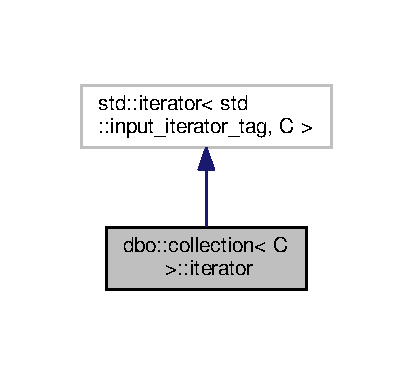
\includegraphics[width=198pt]{classdbo_1_1collection_1_1iterator__inherit__graph}
\end{center}
\end{figure}


Collaboration diagram for dbo\+:\+:collection$<$ C $>$\+:\+:iterator\+:\nopagebreak
\begin{figure}[H]
\begin{center}
\leavevmode
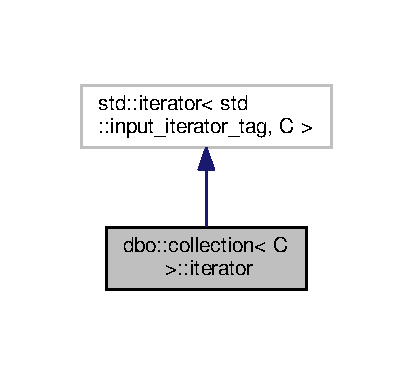
\includegraphics[width=198pt]{classdbo_1_1collection_1_1iterator__coll__graph}
\end{center}
\end{figure}
\subsection*{Public Member Functions}
\begin{DoxyCompactItemize}
\item 
\hyperlink{classdbo_1_1collection_1_1iterator_ab34c352dc47e09471b7873d3a3dc34ae}{iterator} (const \hyperlink{classdbo_1_1collection_1_1iterator}{iterator} \&other)
\begin{DoxyCompactList}\small\item\em Copy constructor. \end{DoxyCompactList}\item 
\hyperlink{classdbo_1_1collection_1_1iterator_a01a082d5caedffa845931334d1828b6f}{$\sim$iterator} ()
\begin{DoxyCompactList}\small\item\em Destructor. \end{DoxyCompactList}\item 
\hyperlink{classdbo_1_1collection_1_1iterator}{iterator} \& \hyperlink{classdbo_1_1collection_1_1iterator_a8e934c72cab4003c8cdfc8cc5b959e7a}{operator=} (const \hyperlink{classdbo_1_1collection_1_1iterator}{iterator} \&other)
\begin{DoxyCompactList}\small\item\em Assignment operator. \end{DoxyCompactList}\item 
\hyperlink{classdbo_1_1ptr}{ptr}$<$ C $>$ \hyperlink{classdbo_1_1collection_1_1iterator_ad3e67a51a801ce5e81ce7581d3813208}{operator$\ast$} ()
\begin{DoxyCompactList}\small\item\em Dereference operator. \end{DoxyCompactList}\item 
\hyperlink{classdbo_1_1ptr}{ptr}$<$ C $>$ $\ast$ \hyperlink{classdbo_1_1collection_1_1iterator_af89d7e4401b7c3689d835a7279b3b896}{operator-\/$>$} ()
\begin{DoxyCompactList}\small\item\em Dereference operator. \end{DoxyCompactList}\item 
bool \hyperlink{classdbo_1_1collection_1_1iterator_af63bc9779f8e27ee1469f287b758016b}{operator==} (const \hyperlink{classdbo_1_1collection_1_1iterator}{iterator} \&other) const 
\begin{DoxyCompactList}\small\item\em Comparison operator. \end{DoxyCompactList}\item 
bool \hyperlink{classdbo_1_1collection_1_1iterator_a0281ee61c1a04ff8fd91e3a0334dc7c8}{operator!=} (const \hyperlink{classdbo_1_1collection_1_1iterator}{iterator} \&other) const 
\begin{DoxyCompactList}\small\item\em Comparison operator. \end{DoxyCompactList}\item 
\hyperlink{classdbo_1_1collection_1_1iterator}{iterator} \& \hyperlink{classdbo_1_1collection_1_1iterator_a2a948aaad2d69c26baf3c85fb529651a}{operator++} ()
\begin{DoxyCompactList}\small\item\em Pre increment operator. \end{DoxyCompactList}\item 
\hyperlink{classdbo_1_1collection_1_1iterator}{iterator} \hyperlink{classdbo_1_1collection_1_1iterator_a55674ea82ad075cf4c726452fb82686b}{operator++} (int)
\begin{DoxyCompactList}\small\item\em Post increment operator. \end{DoxyCompactList}\end{DoxyCompactItemize}
\subsection*{Friends}
\begin{DoxyCompactItemize}
\item 
class \hyperlink{classdbo_1_1collection_1_1iterator_a7d75690b3ffa43c8728bfd4ebacb7cee}{collection$<$ C $>$}
\end{DoxyCompactItemize}


\subsection{Constructor \& Destructor Documentation}
\hypertarget{classdbo_1_1collection_1_1iterator_ab34c352dc47e09471b7873d3a3dc34ae}{\index{dbo\+::collection\+::iterator@{dbo\+::collection\+::iterator}!iterator@{iterator}}
\index{iterator@{iterator}!dbo\+::collection\+::iterator@{dbo\+::collection\+::iterator}}
\subsubsection[{iterator}]{\setlength{\rightskip}{0pt plus 5cm}template$<$class C$>$ {\bf dbo\+::collection}$<$ C $>$\+::iterator\+::iterator (
\begin{DoxyParamCaption}
\item[{const {\bf iterator} \&}]{other}
\end{DoxyParamCaption}
)}}\label{classdbo_1_1collection_1_1iterator_ab34c352dc47e09471b7873d3a3dc34ae}


Copy constructor. 

\hypertarget{classdbo_1_1collection_1_1iterator_a01a082d5caedffa845931334d1828b6f}{\index{dbo\+::collection\+::iterator@{dbo\+::collection\+::iterator}!````~iterator@{$\sim$iterator}}
\index{````~iterator@{$\sim$iterator}!dbo\+::collection\+::iterator@{dbo\+::collection\+::iterator}}
\subsubsection[{$\sim$iterator}]{\setlength{\rightskip}{0pt plus 5cm}template$<$class C $>$ {\bf dbo\+::collection}$<$ C $>$\+::iterator\+::$\sim$iterator (
\begin{DoxyParamCaption}
{}
\end{DoxyParamCaption}
)}}\label{classdbo_1_1collection_1_1iterator_a01a082d5caedffa845931334d1828b6f}


Destructor. 



\subsection{Member Function Documentation}
\hypertarget{classdbo_1_1collection_1_1iterator_a0281ee61c1a04ff8fd91e3a0334dc7c8}{\index{dbo\+::collection\+::iterator@{dbo\+::collection\+::iterator}!operator"!=@{operator"!=}}
\index{operator"!=@{operator"!=}!dbo\+::collection\+::iterator@{dbo\+::collection\+::iterator}}
\subsubsection[{operator"!=}]{\setlength{\rightskip}{0pt plus 5cm}template$<$class C$>$ bool {\bf dbo\+::collection}$<$ C $>$\+::iterator\+::operator!= (
\begin{DoxyParamCaption}
\item[{const {\bf iterator} \&}]{other}
\end{DoxyParamCaption}
) const}}\label{classdbo_1_1collection_1_1iterator_a0281ee61c1a04ff8fd91e3a0334dc7c8}


Comparison operator. 

\hypertarget{classdbo_1_1collection_1_1iterator_ad3e67a51a801ce5e81ce7581d3813208}{\index{dbo\+::collection\+::iterator@{dbo\+::collection\+::iterator}!operator$\ast$@{operator$\ast$}}
\index{operator$\ast$@{operator$\ast$}!dbo\+::collection\+::iterator@{dbo\+::collection\+::iterator}}
\subsubsection[{operator$\ast$}]{\setlength{\rightskip}{0pt plus 5cm}template$<$class C $>$ {\bf ptr}$<$ C $>$ {\bf dbo\+::collection}$<$ C $>$\+::iterator\+::operator$\ast$ (
\begin{DoxyParamCaption}
{}
\end{DoxyParamCaption}
)}}\label{classdbo_1_1collection_1_1iterator_ad3e67a51a801ce5e81ce7581d3813208}


Dereference operator. 

\hypertarget{classdbo_1_1collection_1_1iterator_a2a948aaad2d69c26baf3c85fb529651a}{\index{dbo\+::collection\+::iterator@{dbo\+::collection\+::iterator}!operator++@{operator++}}
\index{operator++@{operator++}!dbo\+::collection\+::iterator@{dbo\+::collection\+::iterator}}
\subsubsection[{operator++}]{\setlength{\rightskip}{0pt plus 5cm}template$<$class C $>$ {\bf collection}$<$ C $>$\+::{\bf iterator} \& {\bf dbo\+::collection}$<$ C $>$\+::iterator\+::operator++ (
\begin{DoxyParamCaption}
{}
\end{DoxyParamCaption}
)}}\label{classdbo_1_1collection_1_1iterator_a2a948aaad2d69c26baf3c85fb529651a}


Pre increment operator. 

\hypertarget{classdbo_1_1collection_1_1iterator_a55674ea82ad075cf4c726452fb82686b}{\index{dbo\+::collection\+::iterator@{dbo\+::collection\+::iterator}!operator++@{operator++}}
\index{operator++@{operator++}!dbo\+::collection\+::iterator@{dbo\+::collection\+::iterator}}
\subsubsection[{operator++}]{\setlength{\rightskip}{0pt plus 5cm}template$<$class C $>$ {\bf collection}$<$ C $>$\+::{\bf iterator} {\bf dbo\+::collection}$<$ C $>$\+::iterator\+::operator++ (
\begin{DoxyParamCaption}
\item[{int}]{value}
\end{DoxyParamCaption}
)}}\label{classdbo_1_1collection_1_1iterator_a55674ea82ad075cf4c726452fb82686b}


Post increment operator. 

\hypertarget{classdbo_1_1collection_1_1iterator_af89d7e4401b7c3689d835a7279b3b896}{\index{dbo\+::collection\+::iterator@{dbo\+::collection\+::iterator}!operator-\/$>$@{operator-\/$>$}}
\index{operator-\/$>$@{operator-\/$>$}!dbo\+::collection\+::iterator@{dbo\+::collection\+::iterator}}
\subsubsection[{operator-\/$>$}]{\setlength{\rightskip}{0pt plus 5cm}template$<$class C $>$ {\bf ptr}$<$ C $>$ $\ast$ {\bf dbo\+::collection}$<$ C $>$\+::iterator\+::operator-\/$>$ (
\begin{DoxyParamCaption}
{}
\end{DoxyParamCaption}
)}}\label{classdbo_1_1collection_1_1iterator_af89d7e4401b7c3689d835a7279b3b896}


Dereference operator. 

\hypertarget{classdbo_1_1collection_1_1iterator_a8e934c72cab4003c8cdfc8cc5b959e7a}{\index{dbo\+::collection\+::iterator@{dbo\+::collection\+::iterator}!operator=@{operator=}}
\index{operator=@{operator=}!dbo\+::collection\+::iterator@{dbo\+::collection\+::iterator}}
\subsubsection[{operator=}]{\setlength{\rightskip}{0pt plus 5cm}template$<$class C$>$ {\bf collection}$<$ C $>$\+::{\bf iterator} \& {\bf dbo\+::collection}$<$ C $>$\+::iterator\+::operator= (
\begin{DoxyParamCaption}
\item[{const {\bf iterator} \&}]{other}
\end{DoxyParamCaption}
)}}\label{classdbo_1_1collection_1_1iterator_a8e934c72cab4003c8cdfc8cc5b959e7a}


Assignment operator. 

\hypertarget{classdbo_1_1collection_1_1iterator_af63bc9779f8e27ee1469f287b758016b}{\index{dbo\+::collection\+::iterator@{dbo\+::collection\+::iterator}!operator==@{operator==}}
\index{operator==@{operator==}!dbo\+::collection\+::iterator@{dbo\+::collection\+::iterator}}
\subsubsection[{operator==}]{\setlength{\rightskip}{0pt plus 5cm}template$<$class C$>$ bool {\bf dbo\+::collection}$<$ C $>$\+::iterator\+::operator== (
\begin{DoxyParamCaption}
\item[{const {\bf iterator} \&}]{other}
\end{DoxyParamCaption}
) const}}\label{classdbo_1_1collection_1_1iterator_af63bc9779f8e27ee1469f287b758016b}


Comparison operator. 

Returns true if two iterators point to the same value in the same collection, or point both to the end of a collection. 

\subsection{Friends And Related Function Documentation}
\hypertarget{classdbo_1_1collection_1_1iterator_a7d75690b3ffa43c8728bfd4ebacb7cee}{\index{dbo\+::collection\+::iterator@{dbo\+::collection\+::iterator}!collection$<$ C $>$@{collection$<$ C $>$}}
\index{collection$<$ C $>$@{collection$<$ C $>$}!dbo\+::collection\+::iterator@{dbo\+::collection\+::iterator}}
\subsubsection[{collection$<$ C $>$}]{\setlength{\rightskip}{0pt plus 5cm}template$<$class C$>$ friend class {\bf collection}$<$ C $>$\hspace{0.3cm}{\ttfamily [friend]}}}\label{classdbo_1_1collection_1_1iterator_a7d75690b3ffa43c8728bfd4ebacb7cee}


The documentation for this class was generated from the following files\+:\begin{DoxyCompactItemize}
\item 
dbo/\hyperlink{collection_8hpp}{collection.\+hpp}\item 
dbo/\hyperlink{collection_8cxx}{collection.\+cxx}\end{DoxyCompactItemize}

\hypertarget{structdbo_1_1mapping_1_1_join_id}{\section{dbo\+:\+:mapping\+:\+:Join\+Id Struct Reference}
\label{structdbo_1_1mapping_1_1_join_id}\index{dbo\+::mapping\+::\+Join\+Id@{dbo\+::mapping\+::\+Join\+Id}}
}


{\ttfamily \#include $<$Join\+Id.\+h$>$}

\subsection*{Public Member Functions}
\begin{DoxyCompactItemize}
\item 
\hyperlink{structdbo_1_1mapping_1_1_join_id_a332b1ffa31b3b93efa14ca17045afd3b}{Join\+Id} (const std\+::string \&a\+Join\+Id\+Name, const std\+::string \&a\+Table\+Id\+Name, const std\+::string \&a\+Sql\+Type)
\end{DoxyCompactItemize}
\subsection*{Public Attributes}
\begin{DoxyCompactItemize}
\item 
std\+::string \hyperlink{structdbo_1_1mapping_1_1_join_id_a7351e903042349c2ea5b3d48c5abbbeb}{join\+Id\+Name}
\item 
std\+::string \hyperlink{structdbo_1_1mapping_1_1_join_id_ae975703316fa343d3410793096a1b17b}{table\+Id\+Name}
\item 
std\+::string \hyperlink{structdbo_1_1mapping_1_1_join_id_a9b3760ce227416a2959251d327ae2665}{sql\+Type}
\end{DoxyCompactItemize}


\subsection{Constructor \& Destructor Documentation}
\hypertarget{structdbo_1_1mapping_1_1_join_id_a332b1ffa31b3b93efa14ca17045afd3b}{\index{dbo\+::mapping\+::\+Join\+Id@{dbo\+::mapping\+::\+Join\+Id}!Join\+Id@{Join\+Id}}
\index{Join\+Id@{Join\+Id}!dbo\+::mapping\+::\+Join\+Id@{dbo\+::mapping\+::\+Join\+Id}}
\subsubsection[{Join\+Id}]{\setlength{\rightskip}{0pt plus 5cm}dbo\+::mapping\+::\+Join\+Id\+::\+Join\+Id (
\begin{DoxyParamCaption}
\item[{const std\+::string \&}]{a\+Join\+Id\+Name, }
\item[{const std\+::string \&}]{a\+Table\+Id\+Name, }
\item[{const std\+::string \&}]{a\+Sql\+Type}
\end{DoxyParamCaption}
)}}\label{structdbo_1_1mapping_1_1_join_id_a332b1ffa31b3b93efa14ca17045afd3b}


\subsection{Member Data Documentation}
\hypertarget{structdbo_1_1mapping_1_1_join_id_a7351e903042349c2ea5b3d48c5abbbeb}{\index{dbo\+::mapping\+::\+Join\+Id@{dbo\+::mapping\+::\+Join\+Id}!join\+Id\+Name@{join\+Id\+Name}}
\index{join\+Id\+Name@{join\+Id\+Name}!dbo\+::mapping\+::\+Join\+Id@{dbo\+::mapping\+::\+Join\+Id}}
\subsubsection[{join\+Id\+Name}]{\setlength{\rightskip}{0pt plus 5cm}std\+::string dbo\+::mapping\+::\+Join\+Id\+::join\+Id\+Name}}\label{structdbo_1_1mapping_1_1_join_id_a7351e903042349c2ea5b3d48c5abbbeb}
\hypertarget{structdbo_1_1mapping_1_1_join_id_a9b3760ce227416a2959251d327ae2665}{\index{dbo\+::mapping\+::\+Join\+Id@{dbo\+::mapping\+::\+Join\+Id}!sql\+Type@{sql\+Type}}
\index{sql\+Type@{sql\+Type}!dbo\+::mapping\+::\+Join\+Id@{dbo\+::mapping\+::\+Join\+Id}}
\subsubsection[{sql\+Type}]{\setlength{\rightskip}{0pt plus 5cm}std\+::string dbo\+::mapping\+::\+Join\+Id\+::sql\+Type}}\label{structdbo_1_1mapping_1_1_join_id_a9b3760ce227416a2959251d327ae2665}
\hypertarget{structdbo_1_1mapping_1_1_join_id_ae975703316fa343d3410793096a1b17b}{\index{dbo\+::mapping\+::\+Join\+Id@{dbo\+::mapping\+::\+Join\+Id}!table\+Id\+Name@{table\+Id\+Name}}
\index{table\+Id\+Name@{table\+Id\+Name}!dbo\+::mapping\+::\+Join\+Id@{dbo\+::mapping\+::\+Join\+Id}}
\subsubsection[{table\+Id\+Name}]{\setlength{\rightskip}{0pt plus 5cm}std\+::string dbo\+::mapping\+::\+Join\+Id\+::table\+Id\+Name}}\label{structdbo_1_1mapping_1_1_join_id_ae975703316fa343d3410793096a1b17b}


The documentation for this struct was generated from the following files\+:\begin{DoxyCompactItemize}
\item 
dbo/mapping/\hyperlink{_join_id_8h}{Join\+Id.\+h}\item 
dbo/mapping/\hyperlink{_join_id_8cpp}{Join\+Id.\+cpp}\end{DoxyCompactItemize}

\hypertarget{classdbo_1_1action_1_1_load_db}{\section{dbo\+:\+:action\+:\+:Load\+Db$<$ C $>$ Class Template Reference}
\label{classdbo_1_1action_1_1_load_db}\index{dbo\+::action\+::\+Load\+Db$<$ C $>$@{dbo\+::action\+::\+Load\+Db$<$ C $>$}}
}


{\ttfamily \#include $<$Load\+Db.\+hpp$>$}

\subsection*{Public Types}
\begin{DoxyCompactItemize}
\item 
using \hyperlink{classdbo_1_1action_1_1_load_db_ab8096fbb7b377363def6103e9dd451a1}{Id\+Type} = typename \hyperlink{structdbo_1_1traits_1_1dbo__traits}{traits\+::dbo\+\_\+traits}$<$ C $>$\+::\hyperlink{classdbo_1_1action_1_1_load_db_ab8096fbb7b377363def6103e9dd451a1}{Id\+Type}
\end{DoxyCompactItemize}
\subsection*{Public Member Functions}
\begin{DoxyCompactItemize}
\item 
\hyperlink{classdbo_1_1action_1_1_load_db_a02817bb6d47c1ecb0d8757333e7bbafd}{Load\+Db} (\hyperlink{classdbo_1_1ptr}{ptr}$<$ C $>$ \&\hyperlink{classdbo_1_1ptr}{ptr}, std\+::shared\+\_\+ptr$<$ \hyperlink{classdbo_1_1mapping_1_1_mapping}{mapping\+::\+Mapping}$<$ C $>$$>$ mapping, \hyperlink{classdbo_1_1stmt_1_1_prepared_statement}{stmt\+::\+Prepared\+Statement} \&stmt)
\item 
void \hyperlink{classdbo_1_1action_1_1_load_db_a7855582f0e69485ec912d0c1f25679cd}{visit} ()
\item 
{\footnotesize template$<$typename V $>$ }\\void \hyperlink{classdbo_1_1action_1_1_load_db_adbc0f146c54ddd386718c86b6959712b}{act} (const \hyperlink{classdbo_1_1mapping_1_1_field_ref}{mapping\+::\+Field\+Ref}$<$ V $>$ \&\hyperlink{namespacedbo_ad1f50f02cb050acf946807959252a93f}{field})
\item 
{\footnotesize template$<$typename V $>$ }\\void \hyperlink{classdbo_1_1action_1_1_load_db_a404185ed719249af30c706eb8fffd140}{act\+Id} (V \&value, const std\+::string \&name, int size)
\item 
{\footnotesize template$<$class D $>$ }\\void \hyperlink{classdbo_1_1action_1_1_load_db_a4e7a6dc0ebc7a03cfbaa8efbd123b838}{act\+Id} (\hyperlink{classdbo_1_1ptr}{ptr}$<$ D $>$ \&value, const std\+::string \&name, int size, int fk\+Constraints)
\item 
{\footnotesize template$<$class D $>$ }\\void \hyperlink{classdbo_1_1action_1_1_load_db_ad3bcb9f15a436f52c6e8c740f7589c5e}{act\+Ptr} (const \hyperlink{classdbo_1_1mapping_1_1_ptr_ref}{mapping\+::\+Ptr\+Ref}$<$ D $>$ \&\hyperlink{namespacedbo_ad1f50f02cb050acf946807959252a93f}{field})
\item 
\hyperlink{classdbo_1_1connection}{connection} \& \hyperlink{classdbo_1_1action_1_1_load_db_a7c262008ee3d1e12b22ba405cd5a989b}{conn} ()
\end{DoxyCompactItemize}
\subsection*{Friends}
\begin{DoxyCompactItemize}
\item 
{\footnotesize template$<$class D $>$ }\\class \hyperlink{classdbo_1_1action_1_1_load_db_addf6451e303d1fec3fb0ffc370b29e81}{Load\+Db}
\end{DoxyCompactItemize}


\subsection{Detailed Description}
\subsubsection*{template$<$class C$>$class dbo\+::action\+::\+Load\+Db$<$ C $>$}

Load an object from statement current state 

\subsection{Member Typedef Documentation}
\hypertarget{classdbo_1_1action_1_1_load_db_ab8096fbb7b377363def6103e9dd451a1}{\index{dbo\+::action\+::\+Load\+Db@{dbo\+::action\+::\+Load\+Db}!Id\+Type@{Id\+Type}}
\index{Id\+Type@{Id\+Type}!dbo\+::action\+::\+Load\+Db@{dbo\+::action\+::\+Load\+Db}}
\subsubsection[{Id\+Type}]{\setlength{\rightskip}{0pt plus 5cm}template$<$class C $>$ using {\bf dbo\+::action\+::\+Load\+Db}$<$ C $>$\+::{\bf Id\+Type} =  typename {\bf traits\+::dbo\+\_\+traits}$<$C$>$\+::{\bf Id\+Type}}}\label{classdbo_1_1action_1_1_load_db_ab8096fbb7b377363def6103e9dd451a1}


\subsection{Constructor \& Destructor Documentation}
\hypertarget{classdbo_1_1action_1_1_load_db_a02817bb6d47c1ecb0d8757333e7bbafd}{\index{dbo\+::action\+::\+Load\+Db@{dbo\+::action\+::\+Load\+Db}!Load\+Db@{Load\+Db}}
\index{Load\+Db@{Load\+Db}!dbo\+::action\+::\+Load\+Db@{dbo\+::action\+::\+Load\+Db}}
\subsubsection[{Load\+Db}]{\setlength{\rightskip}{0pt plus 5cm}template$<$class C $>$ {\bf dbo\+::action\+::\+Load\+Db}$<$ C $>$\+::{\bf Load\+Db} (
\begin{DoxyParamCaption}
\item[{{\bf ptr}$<$ C $>$ \&}]{ptr, }
\item[{std\+::shared\+\_\+ptr$<$ {\bf mapping\+::\+Mapping}$<$ C $>$$>$}]{mapping, }
\item[{{\bf stmt\+::\+Prepared\+Statement} \&}]{stmt}
\end{DoxyParamCaption}
)}}\label{classdbo_1_1action_1_1_load_db_a02817bb6d47c1ecb0d8757333e7bbafd}


\subsection{Member Function Documentation}
\hypertarget{classdbo_1_1action_1_1_load_db_adbc0f146c54ddd386718c86b6959712b}{\index{dbo\+::action\+::\+Load\+Db@{dbo\+::action\+::\+Load\+Db}!act@{act}}
\index{act@{act}!dbo\+::action\+::\+Load\+Db@{dbo\+::action\+::\+Load\+Db}}
\subsubsection[{act}]{\setlength{\rightskip}{0pt plus 5cm}template$<$class C $>$ template$<$typename V $>$ void {\bf dbo\+::action\+::\+Load\+Db}$<$ C $>$\+::act (
\begin{DoxyParamCaption}
\item[{const {\bf mapping\+::\+Field\+Ref}$<$ V $>$ \&}]{field}
\end{DoxyParamCaption}
)}}\label{classdbo_1_1action_1_1_load_db_adbc0f146c54ddd386718c86b6959712b}
\hypertarget{classdbo_1_1action_1_1_load_db_a404185ed719249af30c706eb8fffd140}{\index{dbo\+::action\+::\+Load\+Db@{dbo\+::action\+::\+Load\+Db}!act\+Id@{act\+Id}}
\index{act\+Id@{act\+Id}!dbo\+::action\+::\+Load\+Db@{dbo\+::action\+::\+Load\+Db}}
\subsubsection[{act\+Id}]{\setlength{\rightskip}{0pt plus 5cm}template$<$class C $>$ template$<$typename V $>$ void {\bf dbo\+::action\+::\+Load\+Db}$<$ C $>$\+::act\+Id (
\begin{DoxyParamCaption}
\item[{V \&}]{value, }
\item[{const std\+::string \&}]{name, }
\item[{int}]{size}
\end{DoxyParamCaption}
)}}\label{classdbo_1_1action_1_1_load_db_a404185ed719249af30c706eb8fffd140}
\hypertarget{classdbo_1_1action_1_1_load_db_a4e7a6dc0ebc7a03cfbaa8efbd123b838}{\index{dbo\+::action\+::\+Load\+Db@{dbo\+::action\+::\+Load\+Db}!act\+Id@{act\+Id}}
\index{act\+Id@{act\+Id}!dbo\+::action\+::\+Load\+Db@{dbo\+::action\+::\+Load\+Db}}
\subsubsection[{act\+Id}]{\setlength{\rightskip}{0pt plus 5cm}template$<$class C $>$ template$<$class D $>$ void {\bf dbo\+::action\+::\+Load\+Db}$<$ C $>$\+::act\+Id (
\begin{DoxyParamCaption}
\item[{{\bf ptr}$<$ D $>$ \&}]{value, }
\item[{const std\+::string \&}]{name, }
\item[{int}]{size, }
\item[{int}]{fk\+Constraints}
\end{DoxyParamCaption}
)}}\label{classdbo_1_1action_1_1_load_db_a4e7a6dc0ebc7a03cfbaa8efbd123b838}
\hypertarget{classdbo_1_1action_1_1_load_db_ad3bcb9f15a436f52c6e8c740f7589c5e}{\index{dbo\+::action\+::\+Load\+Db@{dbo\+::action\+::\+Load\+Db}!act\+Ptr@{act\+Ptr}}
\index{act\+Ptr@{act\+Ptr}!dbo\+::action\+::\+Load\+Db@{dbo\+::action\+::\+Load\+Db}}
\subsubsection[{act\+Ptr}]{\setlength{\rightskip}{0pt plus 5cm}template$<$class C $>$ template$<$class D $>$ void {\bf dbo\+::action\+::\+Load\+Db}$<$ C $>$\+::act\+Ptr (
\begin{DoxyParamCaption}
\item[{const {\bf mapping\+::\+Ptr\+Ref}$<$ D $>$ \&}]{field}
\end{DoxyParamCaption}
)}}\label{classdbo_1_1action_1_1_load_db_ad3bcb9f15a436f52c6e8c740f7589c5e}
\hypertarget{classdbo_1_1action_1_1_load_db_a7c262008ee3d1e12b22ba405cd5a989b}{\index{dbo\+::action\+::\+Load\+Db@{dbo\+::action\+::\+Load\+Db}!conn@{conn}}
\index{conn@{conn}!dbo\+::action\+::\+Load\+Db@{dbo\+::action\+::\+Load\+Db}}
\subsubsection[{conn}]{\setlength{\rightskip}{0pt plus 5cm}template$<$class C $>$ {\bf connection}\& {\bf dbo\+::action\+::\+Load\+Db}$<$ C $>$\+::conn (
\begin{DoxyParamCaption}
{}
\end{DoxyParamCaption}
)\hspace{0.3cm}{\ttfamily [inline]}}}\label{classdbo_1_1action_1_1_load_db_a7c262008ee3d1e12b22ba405cd5a989b}
\hypertarget{classdbo_1_1action_1_1_load_db_a7855582f0e69485ec912d0c1f25679cd}{\index{dbo\+::action\+::\+Load\+Db@{dbo\+::action\+::\+Load\+Db}!visit@{visit}}
\index{visit@{visit}!dbo\+::action\+::\+Load\+Db@{dbo\+::action\+::\+Load\+Db}}
\subsubsection[{visit}]{\setlength{\rightskip}{0pt plus 5cm}template$<$class C $>$ void {\bf dbo\+::action\+::\+Load\+Db}$<$ C $>$\+::visit (
\begin{DoxyParamCaption}
{}
\end{DoxyParamCaption}
)}}\label{classdbo_1_1action_1_1_load_db_a7855582f0e69485ec912d0c1f25679cd}


\subsection{Friends And Related Function Documentation}
\hypertarget{classdbo_1_1action_1_1_load_db_addf6451e303d1fec3fb0ffc370b29e81}{\index{dbo\+::action\+::\+Load\+Db@{dbo\+::action\+::\+Load\+Db}!Load\+Db@{Load\+Db}}
\index{Load\+Db@{Load\+Db}!dbo\+::action\+::\+Load\+Db@{dbo\+::action\+::\+Load\+Db}}
\subsubsection[{Load\+Db}]{\setlength{\rightskip}{0pt plus 5cm}template$<$class C $>$ template$<$class D $>$ friend class {\bf Load\+Db}\hspace{0.3cm}{\ttfamily [friend]}}}\label{classdbo_1_1action_1_1_load_db_addf6451e303d1fec3fb0ffc370b29e81}


The documentation for this class was generated from the following files\+:\begin{DoxyCompactItemize}
\item 
dbo/action/\hyperlink{_load_db_8hpp}{Load\+Db.\+hpp}\item 
dbo/action/\hyperlink{_load_db_8cxx}{Load\+Db.\+cxx}\end{DoxyCompactItemize}

\hypertarget{classdbo_1_1mapping_1_1_mapping}{\section{dbo\+:\+:mapping\+:\+:Mapping$<$ T $>$ Class Template Reference}
\label{classdbo_1_1mapping_1_1_mapping}\index{dbo\+::mapping\+::\+Mapping$<$ T $>$@{dbo\+::mapping\+::\+Mapping$<$ T $>$}}
}


{\ttfamily \#include $<$Bulk\+Insert.\+hpp$>$}



Inheritance diagram for dbo\+:\+:mapping\+:\+:Mapping$<$ T $>$\+:\nopagebreak
\begin{figure}[H]
\begin{center}
\leavevmode
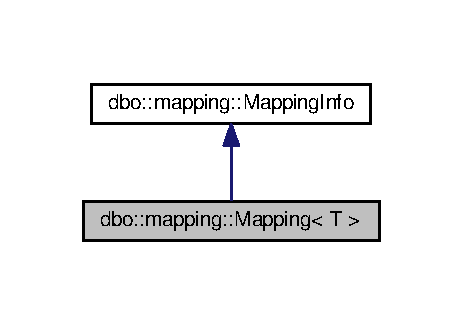
\includegraphics[width=222pt]{classdbo_1_1mapping_1_1_mapping__inherit__graph}
\end{center}
\end{figure}


Collaboration diagram for dbo\+:\+:mapping\+:\+:Mapping$<$ T $>$\+:\nopagebreak
\begin{figure}[H]
\begin{center}
\leavevmode
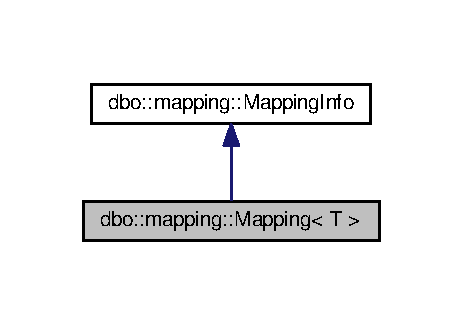
\includegraphics[width=222pt]{classdbo_1_1mapping_1_1_mapping__coll__graph}
\end{center}
\end{figure}
\subsection*{Public Member Functions}
\begin{DoxyCompactItemize}
\item 
\hyperlink{classdbo_1_1mapping_1_1_mapping_a927cfe4cb8b09a4abab992f794ccef7c}{Mapping} ()
\item 
virtual \hyperlink{classdbo_1_1mapping_1_1_mapping_a3e6a13c2c57af34bc24c85ba17fc95a0}{$\sim$\+Mapping} ()
\item 
virtual void \hyperlink{classdbo_1_1mapping_1_1_mapping_a62d1a2cf4a87bda5586012c674178b32}{init} (\hyperlink{classdbo_1_1connection}{connection} \&conn)
\end{DoxyCompactItemize}
\subsection*{Additional Inherited Members}


\subsection{Constructor \& Destructor Documentation}
\hypertarget{classdbo_1_1mapping_1_1_mapping_a927cfe4cb8b09a4abab992f794ccef7c}{\index{dbo\+::mapping\+::\+Mapping@{dbo\+::mapping\+::\+Mapping}!Mapping@{Mapping}}
\index{Mapping@{Mapping}!dbo\+::mapping\+::\+Mapping@{dbo\+::mapping\+::\+Mapping}}
\subsubsection[{Mapping}]{\setlength{\rightskip}{0pt plus 5cm}template$<$class C $>$ {\bf dbo\+::mapping\+::\+Mapping}$<$ C $>$\+::{\bf Mapping} (
\begin{DoxyParamCaption}
{}
\end{DoxyParamCaption}
)}}\label{classdbo_1_1mapping_1_1_mapping_a927cfe4cb8b09a4abab992f794ccef7c}
\hypertarget{classdbo_1_1mapping_1_1_mapping_a3e6a13c2c57af34bc24c85ba17fc95a0}{\index{dbo\+::mapping\+::\+Mapping@{dbo\+::mapping\+::\+Mapping}!````~Mapping@{$\sim$\+Mapping}}
\index{````~Mapping@{$\sim$\+Mapping}!dbo\+::mapping\+::\+Mapping@{dbo\+::mapping\+::\+Mapping}}
\subsubsection[{$\sim$\+Mapping}]{\setlength{\rightskip}{0pt plus 5cm}template$<$class C $>$ {\bf dbo\+::mapping\+::\+Mapping}$<$ C $>$\+::$\sim${\bf Mapping} (
\begin{DoxyParamCaption}
{}
\end{DoxyParamCaption}
)\hspace{0.3cm}{\ttfamily [virtual]}}}\label{classdbo_1_1mapping_1_1_mapping_a3e6a13c2c57af34bc24c85ba17fc95a0}


\subsection{Member Function Documentation}
\hypertarget{classdbo_1_1mapping_1_1_mapping_a62d1a2cf4a87bda5586012c674178b32}{\index{dbo\+::mapping\+::\+Mapping@{dbo\+::mapping\+::\+Mapping}!init@{init}}
\index{init@{init}!dbo\+::mapping\+::\+Mapping@{dbo\+::mapping\+::\+Mapping}}
\subsubsection[{init}]{\setlength{\rightskip}{0pt plus 5cm}template$<$class C $>$ void {\bf dbo\+::mapping\+::\+Mapping}$<$ C $>$\+::init (
\begin{DoxyParamCaption}
\item[{{\bf connection} \&}]{conn}
\end{DoxyParamCaption}
)\hspace{0.3cm}{\ttfamily [virtual]}}}\label{classdbo_1_1mapping_1_1_mapping_a62d1a2cf4a87bda5586012c674178b32}


Reimplemented from \hyperlink{classdbo_1_1mapping_1_1_mapping_info_a1b52b4f58c49b0c7bd64968bae692846}{dbo\+::mapping\+::\+Mapping\+Info}.



The documentation for this class was generated from the following files\+:\begin{DoxyCompactItemize}
\item 
dbo/action/\hyperlink{_bulk_insert_8hpp}{Bulk\+Insert.\+hpp}\item 
dbo/mapping/\hyperlink{_mapping_8hpp}{Mapping.\+hpp}\item 
dbo/mapping/\hyperlink{_mapping_8cxx}{Mapping.\+cxx}\end{DoxyCompactItemize}

\hypertarget{classdbo_1_1mapping_1_1_mapping_info}{\section{dbo\+:\+:mapping\+:\+:Mapping\+Info Class Reference}
\label{classdbo_1_1mapping_1_1_mapping_info}\index{dbo\+::mapping\+::\+Mapping\+Info@{dbo\+::mapping\+::\+Mapping\+Info}}
}


{\ttfamily \#include $<$Mapping\+Info.\+h$>$}



Inheritance diagram for dbo\+:\+:mapping\+:\+:Mapping\+Info\+:\nopagebreak
\begin{figure}[H]
\begin{center}
\leavevmode
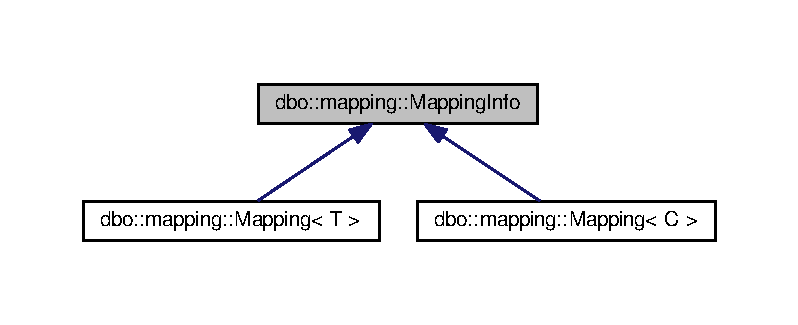
\includegraphics[width=350pt]{classdbo_1_1mapping_1_1_mapping_info__inherit__graph}
\end{center}
\end{figure}
\subsection*{Public Types}
\begin{DoxyCompactItemize}
\item 
enum \hyperlink{classdbo_1_1mapping_1_1_mapping_info_a8edaff7685bc58254cd05ef19ad19c09}{Statement\+Type} \{ \\*
\hyperlink{classdbo_1_1mapping_1_1_mapping_info_a8edaff7685bc58254cd05ef19ad19c09a5f8fdefc757a0babb57069a4190d9ba0}{Sql\+Insert} =0, 
\hyperlink{classdbo_1_1mapping_1_1_mapping_info_a8edaff7685bc58254cd05ef19ad19c09ab1421ced8701f4023a7d3409a5d7e04f}{Sql\+Update} =1, 
\hyperlink{classdbo_1_1mapping_1_1_mapping_info_a8edaff7685bc58254cd05ef19ad19c09a5600f10d886e3eb9c4b8bc2f6becff6d}{Sql\+Delete} =2, 
\hyperlink{classdbo_1_1mapping_1_1_mapping_info_a8edaff7685bc58254cd05ef19ad19c09a2f33d6bb8c5068aab32a5050b5166507}{Sql\+Select\+By\+Id} =3, 
\\*
\hyperlink{classdbo_1_1mapping_1_1_mapping_info_a8edaff7685bc58254cd05ef19ad19c09a9a17045c8f9fecfc4ae978657aa46aca}{First\+Sql\+Select\+Set} =4
 \}
\end{DoxyCompactItemize}
\subsection*{Public Member Functions}
\begin{DoxyCompactItemize}
\item 
\hyperlink{classdbo_1_1mapping_1_1_mapping_info_ae70d8d648ad6a85496e70114c7f621f5}{Mapping\+Info} ()
\item 
virtual \hyperlink{classdbo_1_1mapping_1_1_mapping_info_a0ee09d7f09d6c82b51c0b0d8944d866c}{$\sim$\+Mapping\+Info} ()
\item 
virtual void \hyperlink{classdbo_1_1mapping_1_1_mapping_info_a1b52b4f58c49b0c7bd64968bae692846}{init} (\hyperlink{classdbo_1_1connection}{connection} \&conn)
\item 
std\+::string \hyperlink{classdbo_1_1mapping_1_1_mapping_info_a0fbeeaedf55ac6c78f72ac8eee28fc97}{primary\+Keys} () const 
\item 
std\+::string \hyperlink{classdbo_1_1mapping_1_1_mapping_info_a1285d681d1338c37b003375de2402739}{debug} (int tab)
\end{DoxyCompactItemize}
\subsection*{Public Attributes}
\begin{DoxyCompactItemize}
\item 
bool \hyperlink{classdbo_1_1mapping_1_1_mapping_info_acb52011c465986c42a13d51143810669}{initialized\+\_\+}
\item 
std\+::string \hyperlink{classdbo_1_1mapping_1_1_mapping_info_acbde5a13cfb34bfc295618d04f5e1b2f}{table\+Name}
\item 
boost\+::optional$<$ std\+::string $>$ \hyperlink{classdbo_1_1mapping_1_1_mapping_info_a8748799b225f75d8f8b9921b9a154dc9}{surrogate\+Id\+Field\+Name}
\item 
std\+::string \hyperlink{classdbo_1_1mapping_1_1_mapping_info_af25df5f23a08b2cd0df50e70e1f8153b}{natural\+Id\+Field\+Name}
\item 
int \hyperlink{classdbo_1_1mapping_1_1_mapping_info_a9002b148bddea56eed799ed55577644f}{natural\+Id\+Field\+Size}
\item 
std\+::string \hyperlink{classdbo_1_1mapping_1_1_mapping_info_a1b0c501e1c8b77b950da36250119fb43}{id\+Condition}
\item 
std\+::vector$<$ \hyperlink{classdbo_1_1mapping_1_1_field_info}{Field\+Info} $>$ \hyperlink{classdbo_1_1mapping_1_1_mapping_info_a07655a3c9ed3ada83735b7ab85775dec}{fields}
\item 
std\+::vector$<$ \hyperlink{structdbo_1_1mapping_1_1_set_info}{Set\+Info} $>$ \hyperlink{classdbo_1_1mapping_1_1_mapping_info_aa1aa365dcdf2b60f13bc7fbb9ec11f3f}{sets}
\item 
std\+::map$<$ size\+\_\+t, \\*
\hyperlink{classdbo_1_1stmt_1_1_prepared_statement}{stmt\+::\+Prepared\+Statement} $>$ \hyperlink{classdbo_1_1mapping_1_1_mapping_info_a3049e05c4e13f8d423f84268720602cd}{statements}
\end{DoxyCompactItemize}


\subsection{Member Enumeration Documentation}
\hypertarget{classdbo_1_1mapping_1_1_mapping_info_a8edaff7685bc58254cd05ef19ad19c09}{\index{dbo\+::mapping\+::\+Mapping\+Info@{dbo\+::mapping\+::\+Mapping\+Info}!Statement\+Type@{Statement\+Type}}
\index{Statement\+Type@{Statement\+Type}!dbo\+::mapping\+::\+Mapping\+Info@{dbo\+::mapping\+::\+Mapping\+Info}}
\subsubsection[{Statement\+Type}]{\setlength{\rightskip}{0pt plus 5cm}enum {\bf dbo\+::mapping\+::\+Mapping\+Info\+::\+Statement\+Type}}}\label{classdbo_1_1mapping_1_1_mapping_info_a8edaff7685bc58254cd05ef19ad19c09}
\begin{Desc}
\item[Enumerator]\par
\begin{description}
\index{Sql\+Insert@{Sql\+Insert}!dbo\+::mapping\+::\+Mapping\+Info@{dbo\+::mapping\+::\+Mapping\+Info}}\index{dbo\+::mapping\+::\+Mapping\+Info@{dbo\+::mapping\+::\+Mapping\+Info}!Sql\+Insert@{Sql\+Insert}}\item[{\em 
\hypertarget{classdbo_1_1mapping_1_1_mapping_info_a8edaff7685bc58254cd05ef19ad19c09a5f8fdefc757a0babb57069a4190d9ba0}{Sql\+Insert}\label{classdbo_1_1mapping_1_1_mapping_info_a8edaff7685bc58254cd05ef19ad19c09a5f8fdefc757a0babb57069a4190d9ba0}
}]\index{Sql\+Update@{Sql\+Update}!dbo\+::mapping\+::\+Mapping\+Info@{dbo\+::mapping\+::\+Mapping\+Info}}\index{dbo\+::mapping\+::\+Mapping\+Info@{dbo\+::mapping\+::\+Mapping\+Info}!Sql\+Update@{Sql\+Update}}\item[{\em 
\hypertarget{classdbo_1_1mapping_1_1_mapping_info_a8edaff7685bc58254cd05ef19ad19c09ab1421ced8701f4023a7d3409a5d7e04f}{Sql\+Update}\label{classdbo_1_1mapping_1_1_mapping_info_a8edaff7685bc58254cd05ef19ad19c09ab1421ced8701f4023a7d3409a5d7e04f}
}]\index{Sql\+Delete@{Sql\+Delete}!dbo\+::mapping\+::\+Mapping\+Info@{dbo\+::mapping\+::\+Mapping\+Info}}\index{dbo\+::mapping\+::\+Mapping\+Info@{dbo\+::mapping\+::\+Mapping\+Info}!Sql\+Delete@{Sql\+Delete}}\item[{\em 
\hypertarget{classdbo_1_1mapping_1_1_mapping_info_a8edaff7685bc58254cd05ef19ad19c09a5600f10d886e3eb9c4b8bc2f6becff6d}{Sql\+Delete}\label{classdbo_1_1mapping_1_1_mapping_info_a8edaff7685bc58254cd05ef19ad19c09a5600f10d886e3eb9c4b8bc2f6becff6d}
}]\index{Sql\+Select\+By\+Id@{Sql\+Select\+By\+Id}!dbo\+::mapping\+::\+Mapping\+Info@{dbo\+::mapping\+::\+Mapping\+Info}}\index{dbo\+::mapping\+::\+Mapping\+Info@{dbo\+::mapping\+::\+Mapping\+Info}!Sql\+Select\+By\+Id@{Sql\+Select\+By\+Id}}\item[{\em 
\hypertarget{classdbo_1_1mapping_1_1_mapping_info_a8edaff7685bc58254cd05ef19ad19c09a2f33d6bb8c5068aab32a5050b5166507}{Sql\+Select\+By\+Id}\label{classdbo_1_1mapping_1_1_mapping_info_a8edaff7685bc58254cd05ef19ad19c09a2f33d6bb8c5068aab32a5050b5166507}
}]\index{First\+Sql\+Select\+Set@{First\+Sql\+Select\+Set}!dbo\+::mapping\+::\+Mapping\+Info@{dbo\+::mapping\+::\+Mapping\+Info}}\index{dbo\+::mapping\+::\+Mapping\+Info@{dbo\+::mapping\+::\+Mapping\+Info}!First\+Sql\+Select\+Set@{First\+Sql\+Select\+Set}}\item[{\em 
\hypertarget{classdbo_1_1mapping_1_1_mapping_info_a8edaff7685bc58254cd05ef19ad19c09a9a17045c8f9fecfc4ae978657aa46aca}{First\+Sql\+Select\+Set}\label{classdbo_1_1mapping_1_1_mapping_info_a8edaff7685bc58254cd05ef19ad19c09a9a17045c8f9fecfc4ae978657aa46aca}
}]\end{description}
\end{Desc}


\subsection{Constructor \& Destructor Documentation}
\hypertarget{classdbo_1_1mapping_1_1_mapping_info_ae70d8d648ad6a85496e70114c7f621f5}{\index{dbo\+::mapping\+::\+Mapping\+Info@{dbo\+::mapping\+::\+Mapping\+Info}!Mapping\+Info@{Mapping\+Info}}
\index{Mapping\+Info@{Mapping\+Info}!dbo\+::mapping\+::\+Mapping\+Info@{dbo\+::mapping\+::\+Mapping\+Info}}
\subsubsection[{Mapping\+Info}]{\setlength{\rightskip}{0pt plus 5cm}Mapping\+Info\+::\+Mapping\+Info (
\begin{DoxyParamCaption}
{}
\end{DoxyParamCaption}
)}}\label{classdbo_1_1mapping_1_1_mapping_info_ae70d8d648ad6a85496e70114c7f621f5}
\hypertarget{classdbo_1_1mapping_1_1_mapping_info_a0ee09d7f09d6c82b51c0b0d8944d866c}{\index{dbo\+::mapping\+::\+Mapping\+Info@{dbo\+::mapping\+::\+Mapping\+Info}!````~Mapping\+Info@{$\sim$\+Mapping\+Info}}
\index{````~Mapping\+Info@{$\sim$\+Mapping\+Info}!dbo\+::mapping\+::\+Mapping\+Info@{dbo\+::mapping\+::\+Mapping\+Info}}
\subsubsection[{$\sim$\+Mapping\+Info}]{\setlength{\rightskip}{0pt plus 5cm}Mapping\+Info\+::$\sim$\+Mapping\+Info (
\begin{DoxyParamCaption}
{}
\end{DoxyParamCaption}
)\hspace{0.3cm}{\ttfamily [virtual]}}}\label{classdbo_1_1mapping_1_1_mapping_info_a0ee09d7f09d6c82b51c0b0d8944d866c}


\subsection{Member Function Documentation}
\hypertarget{classdbo_1_1mapping_1_1_mapping_info_a1285d681d1338c37b003375de2402739}{\index{dbo\+::mapping\+::\+Mapping\+Info@{dbo\+::mapping\+::\+Mapping\+Info}!debug@{debug}}
\index{debug@{debug}!dbo\+::mapping\+::\+Mapping\+Info@{dbo\+::mapping\+::\+Mapping\+Info}}
\subsubsection[{debug}]{\setlength{\rightskip}{0pt plus 5cm}std\+::string Mapping\+Info\+::debug (
\begin{DoxyParamCaption}
\item[{int}]{tab}
\end{DoxyParamCaption}
)}}\label{classdbo_1_1mapping_1_1_mapping_info_a1285d681d1338c37b003375de2402739}
\hypertarget{classdbo_1_1mapping_1_1_mapping_info_a1b52b4f58c49b0c7bd64968bae692846}{\index{dbo\+::mapping\+::\+Mapping\+Info@{dbo\+::mapping\+::\+Mapping\+Info}!init@{init}}
\index{init@{init}!dbo\+::mapping\+::\+Mapping\+Info@{dbo\+::mapping\+::\+Mapping\+Info}}
\subsubsection[{init}]{\setlength{\rightskip}{0pt plus 5cm}void Mapping\+Info\+::init (
\begin{DoxyParamCaption}
\item[{{\bf connection} \&}]{conn}
\end{DoxyParamCaption}
)\hspace{0.3cm}{\ttfamily [virtual]}}}\label{classdbo_1_1mapping_1_1_mapping_info_a1b52b4f58c49b0c7bd64968bae692846}


Reimplemented in \hyperlink{classdbo_1_1mapping_1_1_mapping_a62d1a2cf4a87bda5586012c674178b32}{dbo\+::mapping\+::\+Mapping$<$ T $>$}, and \hyperlink{classdbo_1_1mapping_1_1_mapping_a62d1a2cf4a87bda5586012c674178b32}{dbo\+::mapping\+::\+Mapping$<$ C $>$}.

\hypertarget{classdbo_1_1mapping_1_1_mapping_info_a0fbeeaedf55ac6c78f72ac8eee28fc97}{\index{dbo\+::mapping\+::\+Mapping\+Info@{dbo\+::mapping\+::\+Mapping\+Info}!primary\+Keys@{primary\+Keys}}
\index{primary\+Keys@{primary\+Keys}!dbo\+::mapping\+::\+Mapping\+Info@{dbo\+::mapping\+::\+Mapping\+Info}}
\subsubsection[{primary\+Keys}]{\setlength{\rightskip}{0pt plus 5cm}std\+::string Mapping\+Info\+::primary\+Keys (
\begin{DoxyParamCaption}
{}
\end{DoxyParamCaption}
) const}}\label{classdbo_1_1mapping_1_1_mapping_info_a0fbeeaedf55ac6c78f72ac8eee28fc97}


\subsection{Member Data Documentation}
\hypertarget{classdbo_1_1mapping_1_1_mapping_info_a07655a3c9ed3ada83735b7ab85775dec}{\index{dbo\+::mapping\+::\+Mapping\+Info@{dbo\+::mapping\+::\+Mapping\+Info}!fields@{fields}}
\index{fields@{fields}!dbo\+::mapping\+::\+Mapping\+Info@{dbo\+::mapping\+::\+Mapping\+Info}}
\subsubsection[{fields}]{\setlength{\rightskip}{0pt plus 5cm}std\+::vector$<${\bf Field\+Info}$>$ dbo\+::mapping\+::\+Mapping\+Info\+::fields}}\label{classdbo_1_1mapping_1_1_mapping_info_a07655a3c9ed3ada83735b7ab85775dec}
\hypertarget{classdbo_1_1mapping_1_1_mapping_info_a1b0c501e1c8b77b950da36250119fb43}{\index{dbo\+::mapping\+::\+Mapping\+Info@{dbo\+::mapping\+::\+Mapping\+Info}!id\+Condition@{id\+Condition}}
\index{id\+Condition@{id\+Condition}!dbo\+::mapping\+::\+Mapping\+Info@{dbo\+::mapping\+::\+Mapping\+Info}}
\subsubsection[{id\+Condition}]{\setlength{\rightskip}{0pt plus 5cm}std\+::string dbo\+::mapping\+::\+Mapping\+Info\+::id\+Condition}}\label{classdbo_1_1mapping_1_1_mapping_info_a1b0c501e1c8b77b950da36250119fb43}
\hypertarget{classdbo_1_1mapping_1_1_mapping_info_acb52011c465986c42a13d51143810669}{\index{dbo\+::mapping\+::\+Mapping\+Info@{dbo\+::mapping\+::\+Mapping\+Info}!initialized\+\_\+@{initialized\+\_\+}}
\index{initialized\+\_\+@{initialized\+\_\+}!dbo\+::mapping\+::\+Mapping\+Info@{dbo\+::mapping\+::\+Mapping\+Info}}
\subsubsection[{initialized\+\_\+}]{\setlength{\rightskip}{0pt plus 5cm}bool dbo\+::mapping\+::\+Mapping\+Info\+::initialized\+\_\+}}\label{classdbo_1_1mapping_1_1_mapping_info_acb52011c465986c42a13d51143810669}
\hypertarget{classdbo_1_1mapping_1_1_mapping_info_af25df5f23a08b2cd0df50e70e1f8153b}{\index{dbo\+::mapping\+::\+Mapping\+Info@{dbo\+::mapping\+::\+Mapping\+Info}!natural\+Id\+Field\+Name@{natural\+Id\+Field\+Name}}
\index{natural\+Id\+Field\+Name@{natural\+Id\+Field\+Name}!dbo\+::mapping\+::\+Mapping\+Info@{dbo\+::mapping\+::\+Mapping\+Info}}
\subsubsection[{natural\+Id\+Field\+Name}]{\setlength{\rightskip}{0pt plus 5cm}std\+::string dbo\+::mapping\+::\+Mapping\+Info\+::natural\+Id\+Field\+Name}}\label{classdbo_1_1mapping_1_1_mapping_info_af25df5f23a08b2cd0df50e70e1f8153b}
\hypertarget{classdbo_1_1mapping_1_1_mapping_info_a9002b148bddea56eed799ed55577644f}{\index{dbo\+::mapping\+::\+Mapping\+Info@{dbo\+::mapping\+::\+Mapping\+Info}!natural\+Id\+Field\+Size@{natural\+Id\+Field\+Size}}
\index{natural\+Id\+Field\+Size@{natural\+Id\+Field\+Size}!dbo\+::mapping\+::\+Mapping\+Info@{dbo\+::mapping\+::\+Mapping\+Info}}
\subsubsection[{natural\+Id\+Field\+Size}]{\setlength{\rightskip}{0pt plus 5cm}int dbo\+::mapping\+::\+Mapping\+Info\+::natural\+Id\+Field\+Size}}\label{classdbo_1_1mapping_1_1_mapping_info_a9002b148bddea56eed799ed55577644f}
\hypertarget{classdbo_1_1mapping_1_1_mapping_info_aa1aa365dcdf2b60f13bc7fbb9ec11f3f}{\index{dbo\+::mapping\+::\+Mapping\+Info@{dbo\+::mapping\+::\+Mapping\+Info}!sets@{sets}}
\index{sets@{sets}!dbo\+::mapping\+::\+Mapping\+Info@{dbo\+::mapping\+::\+Mapping\+Info}}
\subsubsection[{sets}]{\setlength{\rightskip}{0pt plus 5cm}std\+::vector$<${\bf Set\+Info}$>$ dbo\+::mapping\+::\+Mapping\+Info\+::sets}}\label{classdbo_1_1mapping_1_1_mapping_info_aa1aa365dcdf2b60f13bc7fbb9ec11f3f}
\hypertarget{classdbo_1_1mapping_1_1_mapping_info_a3049e05c4e13f8d423f84268720602cd}{\index{dbo\+::mapping\+::\+Mapping\+Info@{dbo\+::mapping\+::\+Mapping\+Info}!statements@{statements}}
\index{statements@{statements}!dbo\+::mapping\+::\+Mapping\+Info@{dbo\+::mapping\+::\+Mapping\+Info}}
\subsubsection[{statements}]{\setlength{\rightskip}{0pt plus 5cm}std\+::map$<$size\+\_\+t, {\bf stmt\+::\+Prepared\+Statement}$>$ dbo\+::mapping\+::\+Mapping\+Info\+::statements}}\label{classdbo_1_1mapping_1_1_mapping_info_a3049e05c4e13f8d423f84268720602cd}
\hypertarget{classdbo_1_1mapping_1_1_mapping_info_a8748799b225f75d8f8b9921b9a154dc9}{\index{dbo\+::mapping\+::\+Mapping\+Info@{dbo\+::mapping\+::\+Mapping\+Info}!surrogate\+Id\+Field\+Name@{surrogate\+Id\+Field\+Name}}
\index{surrogate\+Id\+Field\+Name@{surrogate\+Id\+Field\+Name}!dbo\+::mapping\+::\+Mapping\+Info@{dbo\+::mapping\+::\+Mapping\+Info}}
\subsubsection[{surrogate\+Id\+Field\+Name}]{\setlength{\rightskip}{0pt plus 5cm}boost\+::optional$<$std\+::string$>$ dbo\+::mapping\+::\+Mapping\+Info\+::surrogate\+Id\+Field\+Name}}\label{classdbo_1_1mapping_1_1_mapping_info_a8748799b225f75d8f8b9921b9a154dc9}
\hypertarget{classdbo_1_1mapping_1_1_mapping_info_acbde5a13cfb34bfc295618d04f5e1b2f}{\index{dbo\+::mapping\+::\+Mapping\+Info@{dbo\+::mapping\+::\+Mapping\+Info}!table\+Name@{table\+Name}}
\index{table\+Name@{table\+Name}!dbo\+::mapping\+::\+Mapping\+Info@{dbo\+::mapping\+::\+Mapping\+Info}}
\subsubsection[{table\+Name}]{\setlength{\rightskip}{0pt plus 5cm}std\+::string dbo\+::mapping\+::\+Mapping\+Info\+::table\+Name}}\label{classdbo_1_1mapping_1_1_mapping_info_acbde5a13cfb34bfc295618d04f5e1b2f}


The documentation for this class was generated from the following files\+:\begin{DoxyCompactItemize}
\item 
dbo/mapping/\hyperlink{_mapping_info_8h}{Mapping\+Info.\+h}\item 
dbo/mapping/\hyperlink{_mapping_info_8cpp}{Mapping\+Info.\+cpp}\end{DoxyCompactItemize}

\hypertarget{classdbo_1_1stmt_1_1_prepared_statement}{\section{dbo\+:\+:stmt\+:\+:Prepared\+Statement Class Reference}
\label{classdbo_1_1stmt_1_1_prepared_statement}\index{dbo\+::stmt\+::\+Prepared\+Statement@{dbo\+::stmt\+::\+Prepared\+Statement}}
}


{\ttfamily \#include $<$Prepared\+Statement.\+h$>$}



Inheritance diagram for dbo\+:\+:stmt\+:\+:Prepared\+Statement\+:\nopagebreak
\begin{figure}[H]
\begin{center}
\leavevmode
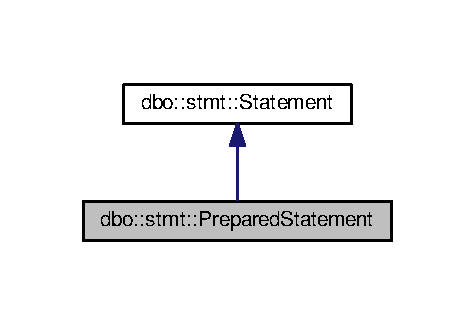
\includegraphics[width=228pt]{classdbo_1_1stmt_1_1_prepared_statement__inherit__graph}
\end{center}
\end{figure}


Collaboration diagram for dbo\+:\+:stmt\+:\+:Prepared\+Statement\+:\nopagebreak
\begin{figure}[H]
\begin{center}
\leavevmode
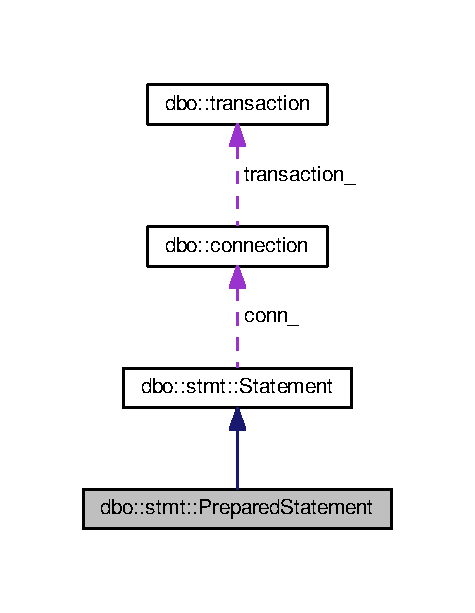
\includegraphics[width=228pt]{classdbo_1_1stmt_1_1_prepared_statement__coll__graph}
\end{center}
\end{figure}
\subsection*{Public Member Functions}
\begin{DoxyCompactItemize}
\item 
\hyperlink{classdbo_1_1stmt_1_1_prepared_statement_a2631fb8e5b366e15a9bb10061572ed51}{Prepared\+Statement} (\hyperlink{classdbo_1_1connection}{connection} \&\hyperlink{classdbo_1_1stmt_1_1_prepared_statement_acb0c5498031d397325904b976581864e}{conn}, std\+::string \hyperlink{classdbo_1_1stmt_1_1_prepared_statement_a5413f8367e7cfcba4a2dfedc11726509}{sql})
\item 
\hyperlink{classdbo_1_1stmt_1_1_prepared_statement_a1bb85967c151e6f56118a9602fecc05c}{Prepared\+Statement} (\hyperlink{classdbo_1_1connection}{connection} \&\hyperlink{classdbo_1_1stmt_1_1_prepared_statement_acb0c5498031d397325904b976581864e}{conn}, std\+::string \hyperlink{classdbo_1_1stmt_1_1_prepared_statement_ad27a0d0ecf8fbe1105ab31d22474a63b}{name}, std\+::string \hyperlink{classdbo_1_1stmt_1_1_prepared_statement_a5413f8367e7cfcba4a2dfedc11726509}{sql})
\item 
virtual \hyperlink{classdbo_1_1stmt_1_1_prepared_statement_a68db1a3435118b1d0c5b083c75ea875c}{$\sim$\+Prepared\+Statement} ()
\item 
void \hyperlink{classdbo_1_1stmt_1_1_prepared_statement_a09a9cd82a4d0123b679312acf74fbd02}{bind} ()
\item 
void \hyperlink{classdbo_1_1stmt_1_1_prepared_statement_a50a8195e7156004c2bf8533a89eb4541}{bind} (const std\+::string \&value)
\item 
void \hyperlink{classdbo_1_1stmt_1_1_prepared_statement_ac569d72f107737acda7ce94c831f5838}{bind} (const std\+::vector$<$ unsigned char $>$ \&value)
\item 
bool \hyperlink{classdbo_1_1stmt_1_1_prepared_statement_ab01ebe611bfdb2a17cc10e7edbb29d4f}{read} (char $\ast$\&value)
\item 
bool \hyperlink{classdbo_1_1stmt_1_1_prepared_statement_a65620d8b28b279d717ed6a787f89ad70}{read} (std\+::vector$<$ unsigned char $>$ \&value)
\item 
void \hyperlink{classdbo_1_1stmt_1_1_prepared_statement_af8ff3a55a05835495670260a71b42fcd}{prepare} ()
\item 
void \hyperlink{classdbo_1_1stmt_1_1_prepared_statement_ac046e6ccc339333d7049ec77bd156f7a}{reset} ()
\item 
void \hyperlink{classdbo_1_1stmt_1_1_prepared_statement_a1f14d39e3ce01f550527b606ec7e16ab}{execute} ()
\item 
bool \hyperlink{classdbo_1_1stmt_1_1_prepared_statement_a8b8b2bcc94ec90843377abafa66e82bb}{next\+Row} ()
\item 
bool \hyperlink{classdbo_1_1stmt_1_1_prepared_statement_a692c0e545c07d818970a208320a03861}{has\+Returning} ()
\item 
const std\+::string \hyperlink{classdbo_1_1stmt_1_1_prepared_statement_a5413f8367e7cfcba4a2dfedc11726509}{sql} () const 
\item 
void \hyperlink{classdbo_1_1stmt_1_1_prepared_statement_ad931d49d80287d23b2effa146a8b2cbc}{sql} (const std\+::string \&sql)
\item 
const std\+::string \hyperlink{classdbo_1_1stmt_1_1_prepared_statement_ad27a0d0ecf8fbe1105ab31d22474a63b}{name} () const 
\item 
void \hyperlink{classdbo_1_1stmt_1_1_prepared_statement_a41a02c96f4fa92db99a7e22dd8544589}{name} (const std\+::string \&name)
\item 
bool \hyperlink{classdbo_1_1stmt_1_1_prepared_statement_a134a6e252ce65627fe0183dee3889118}{hash\+Name} ()
\item 
void \hyperlink{classdbo_1_1stmt_1_1_prepared_statement_a4f037bb4aa0db19d7f1ec282c491d3d3}{hash\+Name} (bool value)
\item 
bool \hyperlink{classdbo_1_1stmt_1_1_prepared_statement_a35dda0d6c5484b0a9ec65a5006262fc0}{prepared} () const 
\item 
\hyperlink{classdbo_1_1connection}{connection} \& \hyperlink{classdbo_1_1stmt_1_1_prepared_statement_acb0c5498031d397325904b976581864e}{conn} () const 
\end{DoxyCompactItemize}
\subsection*{Protected Types}
\begin{DoxyCompactItemize}
\item 
enum \hyperlink{classdbo_1_1stmt_1_1_prepared_statement_a5abdfcba0e0d11c61c0ad555aa7ec053}{O\+I\+D\+Enum} \{ \hyperlink{classdbo_1_1stmt_1_1_prepared_statement_a5abdfcba0e0d11c61c0ad555aa7ec053a2722e683704ee721128f523886c0d5c9}{O\+I\+D\+Default} = 0, 
\hyperlink{classdbo_1_1stmt_1_1_prepared_statement_a5abdfcba0e0d11c61c0ad555aa7ec053a1d0b87b3b8ab7d5f47a4da1b09c44c74}{O\+I\+D\+Bytea} = 17
 \}
\end{DoxyCompactItemize}
\subsection*{Protected Member Functions}
\begin{DoxyCompactItemize}
\item 
std\+::string \hyperlink{classdbo_1_1stmt_1_1_prepared_statement_a791835c0fb71225cd2c1bd8dd576b247}{convert\+To\+Numbered\+Placeholders} (const std\+::string \&\hyperlink{classdbo_1_1stmt_1_1_prepared_statement_a5413f8367e7cfcba4a2dfedc11726509}{sql})
\item 
size\+\_\+t \hyperlink{classdbo_1_1stmt_1_1_prepared_statement_a9e094e897a46d7876081c58eab3c8a0c}{get\+Number\+Place\+Holders} (const std\+::string \&\hyperlink{classdbo_1_1stmt_1_1_prepared_statement_a5413f8367e7cfcba4a2dfedc11726509}{sql})
\item 
size\+\_\+t \hyperlink{classdbo_1_1stmt_1_1_prepared_statement_ae50936c7ba9f917080a85b16008b0ff3}{get\+Place\+Holders} (const std\+::string \&\hyperlink{classdbo_1_1stmt_1_1_prepared_statement_a5413f8367e7cfcba4a2dfedc11726509}{sql}, std\+::map$<$ std\+::string, std\+::string $>$ \&placeholders)
\item 
std\+::string \hyperlink{classdbo_1_1stmt_1_1_prepared_statement_a647184158cda629d94c8e4dc49b245b8}{get\+Bound\+Placeholders} ()
\end{DoxyCompactItemize}
\subsection*{Static Protected Member Functions}
\begin{DoxyCompactItemize}
\item 
static void \hyperlink{classdbo_1_1stmt_1_1_prepared_statement_a52ad363c227383fefab22260545affea}{pg\+\_\+result\+\_\+deleter} (pg\+\_\+result $\ast$result)
\end{DoxyCompactItemize}
\subsection*{Protected Attributes}
\begin{DoxyCompactItemize}
\item 
bool \hyperlink{classdbo_1_1stmt_1_1_prepared_statement_a5ce77cce92c44e28439c8a48d82d49c0}{hashname\+\_\+}
\item 
std\+::string \hyperlink{classdbo_1_1stmt_1_1_prepared_statement_a2a9f1924623015da69452ee4a76a8c95}{name\+\_\+}
\item 
std\+::string \hyperlink{classdbo_1_1stmt_1_1_prepared_statement_ae40cc1d7bed1014bddb5c3ea26cbbc22}{rawsql\+\_\+}
\item 
std\+::string \hyperlink{classdbo_1_1stmt_1_1_prepared_statement_af86636880d2769856602206df3f6b745}{sql\+\_\+}
\item 
bool \hyperlink{classdbo_1_1stmt_1_1_prepared_statement_a7657f4e518a93c0b9b437f7e616cf45d}{prepared\+\_\+}
\item 
size\+\_\+t \hyperlink{classdbo_1_1stmt_1_1_prepared_statement_af124f6fa66f785968da90ab0c1c65862}{param\+Count\+\_\+}
\item 
std\+::shared\+\_\+ptr$<$ pg\+\_\+result $>$ \hyperlink{classdbo_1_1stmt_1_1_prepared_statement_ab069cf8eedb47bd9ac0ee6d5b24e2afb}{result\+\_\+}
\item 
int \hyperlink{classdbo_1_1stmt_1_1_prepared_statement_a65f197eaa23cb862ac56009d8ca18e60}{row\+\_\+}
\item 
int \hyperlink{classdbo_1_1stmt_1_1_prepared_statement_afb28c6676ebd608932654dde2722eae8}{column\+\_\+}
\item 
size\+\_\+t \hyperlink{classdbo_1_1stmt_1_1_prepared_statement_acf79026811fc4238d5bbd50283029be6}{affected\+Rows\+\_\+}
\item 
bool \hyperlink{classdbo_1_1stmt_1_1_prepared_statement_a2eb8c6d22ad2f31295fe41a9c5cfffc8}{has\+Returning\+\_\+}
\item 
std\+::vector$<$ unsigned int $>$ \hyperlink{classdbo_1_1stmt_1_1_prepared_statement_a84dc480075707811e5b4122fdff08615}{oids\+\_\+}
\item 
std\+::vector$<$ std\+::string $>$ \hyperlink{classdbo_1_1stmt_1_1_prepared_statement_a312b978fcd4467e19aba95f944d9e76c}{svalues\+\_\+}
\item 
std\+::vector$<$ const char $\ast$ $>$ \hyperlink{classdbo_1_1stmt_1_1_prepared_statement_a125336886e5cd1e39fd5711b0c91c902}{values\+\_\+}
\item 
std\+::vector$<$ int $>$ \hyperlink{classdbo_1_1stmt_1_1_prepared_statement_a8bf1e4037693e44dbaebffcd1f312c0d}{lengths\+\_\+}
\item 
std\+::vector$<$ int $>$ \hyperlink{classdbo_1_1stmt_1_1_prepared_statement_a2e95148521796406741f62077f3a5576}{formats\+\_\+}
\end{DoxyCompactItemize}


\subsection{Member Enumeration Documentation}
\hypertarget{classdbo_1_1stmt_1_1_prepared_statement_a5abdfcba0e0d11c61c0ad555aa7ec053}{\index{dbo\+::stmt\+::\+Prepared\+Statement@{dbo\+::stmt\+::\+Prepared\+Statement}!O\+I\+D\+Enum@{O\+I\+D\+Enum}}
\index{O\+I\+D\+Enum@{O\+I\+D\+Enum}!dbo\+::stmt\+::\+Prepared\+Statement@{dbo\+::stmt\+::\+Prepared\+Statement}}
\subsubsection[{O\+I\+D\+Enum}]{\setlength{\rightskip}{0pt plus 5cm}enum {\bf dbo\+::stmt\+::\+Prepared\+Statement\+::\+O\+I\+D\+Enum}\hspace{0.3cm}{\ttfamily [protected]}}}\label{classdbo_1_1stmt_1_1_prepared_statement_a5abdfcba0e0d11c61c0ad555aa7ec053}
\begin{Desc}
\item[Enumerator]\par
\begin{description}
\index{O\+I\+D\+Default@{O\+I\+D\+Default}!dbo\+::stmt\+::\+Prepared\+Statement@{dbo\+::stmt\+::\+Prepared\+Statement}}\index{dbo\+::stmt\+::\+Prepared\+Statement@{dbo\+::stmt\+::\+Prepared\+Statement}!O\+I\+D\+Default@{O\+I\+D\+Default}}\item[{\em 
\hypertarget{classdbo_1_1stmt_1_1_prepared_statement_a5abdfcba0e0d11c61c0ad555aa7ec053a2722e683704ee721128f523886c0d5c9}{O\+I\+D\+Default}\label{classdbo_1_1stmt_1_1_prepared_statement_a5abdfcba0e0d11c61c0ad555aa7ec053a2722e683704ee721128f523886c0d5c9}
}]\index{O\+I\+D\+Bytea@{O\+I\+D\+Bytea}!dbo\+::stmt\+::\+Prepared\+Statement@{dbo\+::stmt\+::\+Prepared\+Statement}}\index{dbo\+::stmt\+::\+Prepared\+Statement@{dbo\+::stmt\+::\+Prepared\+Statement}!O\+I\+D\+Bytea@{O\+I\+D\+Bytea}}\item[{\em 
\hypertarget{classdbo_1_1stmt_1_1_prepared_statement_a5abdfcba0e0d11c61c0ad555aa7ec053a1d0b87b3b8ab7d5f47a4da1b09c44c74}{O\+I\+D\+Bytea}\label{classdbo_1_1stmt_1_1_prepared_statement_a5abdfcba0e0d11c61c0ad555aa7ec053a1d0b87b3b8ab7d5f47a4da1b09c44c74}
}]\end{description}
\end{Desc}


\subsection{Constructor \& Destructor Documentation}
\hypertarget{classdbo_1_1stmt_1_1_prepared_statement_a2631fb8e5b366e15a9bb10061572ed51}{\index{dbo\+::stmt\+::\+Prepared\+Statement@{dbo\+::stmt\+::\+Prepared\+Statement}!Prepared\+Statement@{Prepared\+Statement}}
\index{Prepared\+Statement@{Prepared\+Statement}!dbo\+::stmt\+::\+Prepared\+Statement@{dbo\+::stmt\+::\+Prepared\+Statement}}
\subsubsection[{Prepared\+Statement}]{\setlength{\rightskip}{0pt plus 5cm}Prepared\+Statement\+::\+Prepared\+Statement (
\begin{DoxyParamCaption}
\item[{{\bf connection} \&}]{conn, }
\item[{std\+::string}]{sql}
\end{DoxyParamCaption}
)}}\label{classdbo_1_1stmt_1_1_prepared_statement_a2631fb8e5b366e15a9bb10061572ed51}
Build a statement, the name of the statement will be created from the hash of the sql query \hypertarget{classdbo_1_1stmt_1_1_prepared_statement_a1bb85967c151e6f56118a9602fecc05c}{\index{dbo\+::stmt\+::\+Prepared\+Statement@{dbo\+::stmt\+::\+Prepared\+Statement}!Prepared\+Statement@{Prepared\+Statement}}
\index{Prepared\+Statement@{Prepared\+Statement}!dbo\+::stmt\+::\+Prepared\+Statement@{dbo\+::stmt\+::\+Prepared\+Statement}}
\subsubsection[{Prepared\+Statement}]{\setlength{\rightskip}{0pt plus 5cm}Prepared\+Statement\+::\+Prepared\+Statement (
\begin{DoxyParamCaption}
\item[{{\bf connection} \&}]{conn, }
\item[{std\+::string}]{name, }
\item[{std\+::string}]{sql}
\end{DoxyParamCaption}
)}}\label{classdbo_1_1stmt_1_1_prepared_statement_a1bb85967c151e6f56118a9602fecc05c}
Build a statement. If the given name is empty then the statement is treated as an anonymous statement and will overwrite any previous anonymous statement \hypertarget{classdbo_1_1stmt_1_1_prepared_statement_a68db1a3435118b1d0c5b083c75ea875c}{\index{dbo\+::stmt\+::\+Prepared\+Statement@{dbo\+::stmt\+::\+Prepared\+Statement}!````~Prepared\+Statement@{$\sim$\+Prepared\+Statement}}
\index{````~Prepared\+Statement@{$\sim$\+Prepared\+Statement}!dbo\+::stmt\+::\+Prepared\+Statement@{dbo\+::stmt\+::\+Prepared\+Statement}}
\subsubsection[{$\sim$\+Prepared\+Statement}]{\setlength{\rightskip}{0pt plus 5cm}Prepared\+Statement\+::$\sim$\+Prepared\+Statement (
\begin{DoxyParamCaption}
{}
\end{DoxyParamCaption}
)\hspace{0.3cm}{\ttfamily [virtual]}}}\label{classdbo_1_1stmt_1_1_prepared_statement_a68db1a3435118b1d0c5b083c75ea875c}


\subsection{Member Function Documentation}
\hypertarget{classdbo_1_1stmt_1_1_prepared_statement_a09a9cd82a4d0123b679312acf74fbd02}{\index{dbo\+::stmt\+::\+Prepared\+Statement@{dbo\+::stmt\+::\+Prepared\+Statement}!bind@{bind}}
\index{bind@{bind}!dbo\+::stmt\+::\+Prepared\+Statement@{dbo\+::stmt\+::\+Prepared\+Statement}}
\subsubsection[{bind}]{\setlength{\rightskip}{0pt plus 5cm}void Prepared\+Statement\+::bind (
\begin{DoxyParamCaption}
{}
\end{DoxyParamCaption}
)\hspace{0.3cm}{\ttfamily [virtual]}}}\label{classdbo_1_1stmt_1_1_prepared_statement_a09a9cd82a4d0123b679312acf74fbd02}
A statement is copyable under conditions. You can only copy prepared statements, statements with results will throw an error. You can copy a statement only if it is from the same connection Bind a null value 

Implements \hyperlink{classdbo_1_1stmt_1_1_statement_a1699d7873785908a99211c91350cd376}{dbo\+::stmt\+::\+Statement}.

\hypertarget{classdbo_1_1stmt_1_1_prepared_statement_a50a8195e7156004c2bf8533a89eb4541}{\index{dbo\+::stmt\+::\+Prepared\+Statement@{dbo\+::stmt\+::\+Prepared\+Statement}!bind@{bind}}
\index{bind@{bind}!dbo\+::stmt\+::\+Prepared\+Statement@{dbo\+::stmt\+::\+Prepared\+Statement}}
\subsubsection[{bind}]{\setlength{\rightskip}{0pt plus 5cm}void Prepared\+Statement\+::bind (
\begin{DoxyParamCaption}
\item[{const std\+::string \&}]{value}
\end{DoxyParamCaption}
)\hspace{0.3cm}{\ttfamily [virtual]}}}\label{classdbo_1_1stmt_1_1_prepared_statement_a50a8195e7156004c2bf8533a89eb4541}
Bind a string value 

Implements \hyperlink{classdbo_1_1stmt_1_1_statement_a8f2897467f5fccaec72ffe5ad797a8a3}{dbo\+::stmt\+::\+Statement}.

\hypertarget{classdbo_1_1stmt_1_1_prepared_statement_ac569d72f107737acda7ce94c831f5838}{\index{dbo\+::stmt\+::\+Prepared\+Statement@{dbo\+::stmt\+::\+Prepared\+Statement}!bind@{bind}}
\index{bind@{bind}!dbo\+::stmt\+::\+Prepared\+Statement@{dbo\+::stmt\+::\+Prepared\+Statement}}
\subsubsection[{bind}]{\setlength{\rightskip}{0pt plus 5cm}void Prepared\+Statement\+::bind (
\begin{DoxyParamCaption}
\item[{const std\+::vector$<$ unsigned char $>$ \&}]{value}
\end{DoxyParamCaption}
)\hspace{0.3cm}{\ttfamily [virtual]}}}\label{classdbo_1_1stmt_1_1_prepared_statement_ac569d72f107737acda7ce94c831f5838}
Bind a binary value 

Implements \hyperlink{classdbo_1_1stmt_1_1_statement_a3f4f506b3df6f2d8667fa2900a662ee4}{dbo\+::stmt\+::\+Statement}.

\hypertarget{classdbo_1_1stmt_1_1_prepared_statement_acb0c5498031d397325904b976581864e}{\index{dbo\+::stmt\+::\+Prepared\+Statement@{dbo\+::stmt\+::\+Prepared\+Statement}!conn@{conn}}
\index{conn@{conn}!dbo\+::stmt\+::\+Prepared\+Statement@{dbo\+::stmt\+::\+Prepared\+Statement}}
\subsubsection[{conn}]{\setlength{\rightskip}{0pt plus 5cm}{\bf connection}\& dbo\+::stmt\+::\+Prepared\+Statement\+::conn (
\begin{DoxyParamCaption}
{}
\end{DoxyParamCaption}
) const\hspace{0.3cm}{\ttfamily [inline]}}}\label{classdbo_1_1stmt_1_1_prepared_statement_acb0c5498031d397325904b976581864e}
\hypertarget{classdbo_1_1stmt_1_1_prepared_statement_a791835c0fb71225cd2c1bd8dd576b247}{\index{dbo\+::stmt\+::\+Prepared\+Statement@{dbo\+::stmt\+::\+Prepared\+Statement}!convert\+To\+Numbered\+Placeholders@{convert\+To\+Numbered\+Placeholders}}
\index{convert\+To\+Numbered\+Placeholders@{convert\+To\+Numbered\+Placeholders}!dbo\+::stmt\+::\+Prepared\+Statement@{dbo\+::stmt\+::\+Prepared\+Statement}}
\subsubsection[{convert\+To\+Numbered\+Placeholders}]{\setlength{\rightskip}{0pt plus 5cm}std\+::string Prepared\+Statement\+::convert\+To\+Numbered\+Placeholders (
\begin{DoxyParamCaption}
\item[{const std\+::string \&}]{sql}
\end{DoxyParamCaption}
)\hspace{0.3cm}{\ttfamily [protected]}}}\label{classdbo_1_1stmt_1_1_prepared_statement_a791835c0fb71225cd2c1bd8dd576b247}
\hypertarget{classdbo_1_1stmt_1_1_prepared_statement_a1f14d39e3ce01f550527b606ec7e16ab}{\index{dbo\+::stmt\+::\+Prepared\+Statement@{dbo\+::stmt\+::\+Prepared\+Statement}!execute@{execute}}
\index{execute@{execute}!dbo\+::stmt\+::\+Prepared\+Statement@{dbo\+::stmt\+::\+Prepared\+Statement}}
\subsubsection[{execute}]{\setlength{\rightskip}{0pt plus 5cm}void Prepared\+Statement\+::execute (
\begin{DoxyParamCaption}
{}
\end{DoxyParamCaption}
)\hspace{0.3cm}{\ttfamily [virtual]}}}\label{classdbo_1_1stmt_1_1_prepared_statement_a1f14d39e3ce01f550527b606ec7e16ab}
Execute the prepared statement 

Implements \hyperlink{classdbo_1_1stmt_1_1_statement_af8e1a95b6c0c8b8ac6f5a25f4c48bf5e}{dbo\+::stmt\+::\+Statement}.

\hypertarget{classdbo_1_1stmt_1_1_prepared_statement_a647184158cda629d94c8e4dc49b245b8}{\index{dbo\+::stmt\+::\+Prepared\+Statement@{dbo\+::stmt\+::\+Prepared\+Statement}!get\+Bound\+Placeholders@{get\+Bound\+Placeholders}}
\index{get\+Bound\+Placeholders@{get\+Bound\+Placeholders}!dbo\+::stmt\+::\+Prepared\+Statement@{dbo\+::stmt\+::\+Prepared\+Statement}}
\subsubsection[{get\+Bound\+Placeholders}]{\setlength{\rightskip}{0pt plus 5cm}std\+::string Prepared\+Statement\+::get\+Bound\+Placeholders (
\begin{DoxyParamCaption}
{}
\end{DoxyParamCaption}
)\hspace{0.3cm}{\ttfamily [protected]}}}\label{classdbo_1_1stmt_1_1_prepared_statement_a647184158cda629d94c8e4dc49b245b8}
\hypertarget{classdbo_1_1stmt_1_1_prepared_statement_a9e094e897a46d7876081c58eab3c8a0c}{\index{dbo\+::stmt\+::\+Prepared\+Statement@{dbo\+::stmt\+::\+Prepared\+Statement}!get\+Number\+Place\+Holders@{get\+Number\+Place\+Holders}}
\index{get\+Number\+Place\+Holders@{get\+Number\+Place\+Holders}!dbo\+::stmt\+::\+Prepared\+Statement@{dbo\+::stmt\+::\+Prepared\+Statement}}
\subsubsection[{get\+Number\+Place\+Holders}]{\setlength{\rightskip}{0pt plus 5cm}size\+\_\+t Prepared\+Statement\+::get\+Number\+Place\+Holders (
\begin{DoxyParamCaption}
\item[{const std\+::string \&}]{sql}
\end{DoxyParamCaption}
)\hspace{0.3cm}{\ttfamily [protected]}}}\label{classdbo_1_1stmt_1_1_prepared_statement_a9e094e897a46d7876081c58eab3c8a0c}
\hypertarget{classdbo_1_1stmt_1_1_prepared_statement_ae50936c7ba9f917080a85b16008b0ff3}{\index{dbo\+::stmt\+::\+Prepared\+Statement@{dbo\+::stmt\+::\+Prepared\+Statement}!get\+Place\+Holders@{get\+Place\+Holders}}
\index{get\+Place\+Holders@{get\+Place\+Holders}!dbo\+::stmt\+::\+Prepared\+Statement@{dbo\+::stmt\+::\+Prepared\+Statement}}
\subsubsection[{get\+Place\+Holders}]{\setlength{\rightskip}{0pt plus 5cm}size\+\_\+t Prepared\+Statement\+::get\+Place\+Holders (
\begin{DoxyParamCaption}
\item[{const std\+::string \&}]{sql, }
\item[{std\+::map$<$ std\+::string, std\+::string $>$ \&}]{placeholders}
\end{DoxyParamCaption}
)\hspace{0.3cm}{\ttfamily [protected]}}}\label{classdbo_1_1stmt_1_1_prepared_statement_ae50936c7ba9f917080a85b16008b0ff3}
\hypertarget{classdbo_1_1stmt_1_1_prepared_statement_a134a6e252ce65627fe0183dee3889118}{\index{dbo\+::stmt\+::\+Prepared\+Statement@{dbo\+::stmt\+::\+Prepared\+Statement}!hash\+Name@{hash\+Name}}
\index{hash\+Name@{hash\+Name}!dbo\+::stmt\+::\+Prepared\+Statement@{dbo\+::stmt\+::\+Prepared\+Statement}}
\subsubsection[{hash\+Name}]{\setlength{\rightskip}{0pt plus 5cm}bool dbo\+::stmt\+::\+Prepared\+Statement\+::hash\+Name (
\begin{DoxyParamCaption}
{}
\end{DoxyParamCaption}
)\hspace{0.3cm}{\ttfamily [inline]}}}\label{classdbo_1_1stmt_1_1_prepared_statement_a134a6e252ce65627fe0183dee3889118}
\hypertarget{classdbo_1_1stmt_1_1_prepared_statement_a4f037bb4aa0db19d7f1ec282c491d3d3}{\index{dbo\+::stmt\+::\+Prepared\+Statement@{dbo\+::stmt\+::\+Prepared\+Statement}!hash\+Name@{hash\+Name}}
\index{hash\+Name@{hash\+Name}!dbo\+::stmt\+::\+Prepared\+Statement@{dbo\+::stmt\+::\+Prepared\+Statement}}
\subsubsection[{hash\+Name}]{\setlength{\rightskip}{0pt plus 5cm}void Prepared\+Statement\+::hash\+Name (
\begin{DoxyParamCaption}
\item[{bool}]{value}
\end{DoxyParamCaption}
)}}\label{classdbo_1_1stmt_1_1_prepared_statement_a4f037bb4aa0db19d7f1ec282c491d3d3}
\hypertarget{classdbo_1_1stmt_1_1_prepared_statement_a692c0e545c07d818970a208320a03861}{\index{dbo\+::stmt\+::\+Prepared\+Statement@{dbo\+::stmt\+::\+Prepared\+Statement}!has\+Returning@{has\+Returning}}
\index{has\+Returning@{has\+Returning}!dbo\+::stmt\+::\+Prepared\+Statement@{dbo\+::stmt\+::\+Prepared\+Statement}}
\subsubsection[{has\+Returning}]{\setlength{\rightskip}{0pt plus 5cm}bool dbo\+::stmt\+::\+Prepared\+Statement\+::has\+Returning (
\begin{DoxyParamCaption}
{}
\end{DoxyParamCaption}
)\hspace{0.3cm}{\ttfamily [inline]}}}\label{classdbo_1_1stmt_1_1_prepared_statement_a692c0e545c07d818970a208320a03861}
Indicate if an insert has a returning \hypertarget{classdbo_1_1stmt_1_1_prepared_statement_ad27a0d0ecf8fbe1105ab31d22474a63b}{\index{dbo\+::stmt\+::\+Prepared\+Statement@{dbo\+::stmt\+::\+Prepared\+Statement}!name@{name}}
\index{name@{name}!dbo\+::stmt\+::\+Prepared\+Statement@{dbo\+::stmt\+::\+Prepared\+Statement}}
\subsubsection[{name}]{\setlength{\rightskip}{0pt plus 5cm}const std\+::string dbo\+::stmt\+::\+Prepared\+Statement\+::name (
\begin{DoxyParamCaption}
{}
\end{DoxyParamCaption}
) const\hspace{0.3cm}{\ttfamily [inline]}}}\label{classdbo_1_1stmt_1_1_prepared_statement_ad27a0d0ecf8fbe1105ab31d22474a63b}
\hypertarget{classdbo_1_1stmt_1_1_prepared_statement_a41a02c96f4fa92db99a7e22dd8544589}{\index{dbo\+::stmt\+::\+Prepared\+Statement@{dbo\+::stmt\+::\+Prepared\+Statement}!name@{name}}
\index{name@{name}!dbo\+::stmt\+::\+Prepared\+Statement@{dbo\+::stmt\+::\+Prepared\+Statement}}
\subsubsection[{name}]{\setlength{\rightskip}{0pt plus 5cm}void Prepared\+Statement\+::name (
\begin{DoxyParamCaption}
\item[{const std\+::string \&}]{name}
\end{DoxyParamCaption}
)}}\label{classdbo_1_1stmt_1_1_prepared_statement_a41a02c96f4fa92db99a7e22dd8544589}
Set name of prepared statement If name is empty then prepared statement is anonymous and will overwrite previous prepared anonymous statement at prepare. \hypertarget{classdbo_1_1stmt_1_1_prepared_statement_a8b8b2bcc94ec90843377abafa66e82bb}{\index{dbo\+::stmt\+::\+Prepared\+Statement@{dbo\+::stmt\+::\+Prepared\+Statement}!next\+Row@{next\+Row}}
\index{next\+Row@{next\+Row}!dbo\+::stmt\+::\+Prepared\+Statement@{dbo\+::stmt\+::\+Prepared\+Statement}}
\subsubsection[{next\+Row}]{\setlength{\rightskip}{0pt plus 5cm}bool Prepared\+Statement\+::next\+Row (
\begin{DoxyParamCaption}
{}
\end{DoxyParamCaption}
)}}\label{classdbo_1_1stmt_1_1_prepared_statement_a8b8b2bcc94ec90843377abafa66e82bb}
\hypertarget{classdbo_1_1stmt_1_1_prepared_statement_a52ad363c227383fefab22260545affea}{\index{dbo\+::stmt\+::\+Prepared\+Statement@{dbo\+::stmt\+::\+Prepared\+Statement}!pg\+\_\+result\+\_\+deleter@{pg\+\_\+result\+\_\+deleter}}
\index{pg\+\_\+result\+\_\+deleter@{pg\+\_\+result\+\_\+deleter}!dbo\+::stmt\+::\+Prepared\+Statement@{dbo\+::stmt\+::\+Prepared\+Statement}}
\subsubsection[{pg\+\_\+result\+\_\+deleter}]{\setlength{\rightskip}{0pt plus 5cm}void Prepared\+Statement\+::pg\+\_\+result\+\_\+deleter (
\begin{DoxyParamCaption}
\item[{pg\+\_\+result $\ast$}]{result}
\end{DoxyParamCaption}
)\hspace{0.3cm}{\ttfamily [static]}, {\ttfamily [protected]}}}\label{classdbo_1_1stmt_1_1_prepared_statement_a52ad363c227383fefab22260545affea}
\hypertarget{classdbo_1_1stmt_1_1_prepared_statement_af8ff3a55a05835495670260a71b42fcd}{\index{dbo\+::stmt\+::\+Prepared\+Statement@{dbo\+::stmt\+::\+Prepared\+Statement}!prepare@{prepare}}
\index{prepare@{prepare}!dbo\+::stmt\+::\+Prepared\+Statement@{dbo\+::stmt\+::\+Prepared\+Statement}}
\subsubsection[{prepare}]{\setlength{\rightskip}{0pt plus 5cm}void Prepared\+Statement\+::prepare (
\begin{DoxyParamCaption}
{}
\end{DoxyParamCaption}
)}}\label{classdbo_1_1stmt_1_1_prepared_statement_af8ff3a55a05835495670260a71b42fcd}
Prepare the statement and registers it Uses the bound values to chose the right oids N\+U\+L\+L values binds to O\+I\+D\+Default bind count must be equal to request parameters number \hypertarget{classdbo_1_1stmt_1_1_prepared_statement_a35dda0d6c5484b0a9ec65a5006262fc0}{\index{dbo\+::stmt\+::\+Prepared\+Statement@{dbo\+::stmt\+::\+Prepared\+Statement}!prepared@{prepared}}
\index{prepared@{prepared}!dbo\+::stmt\+::\+Prepared\+Statement@{dbo\+::stmt\+::\+Prepared\+Statement}}
\subsubsection[{prepared}]{\setlength{\rightskip}{0pt plus 5cm}bool dbo\+::stmt\+::\+Prepared\+Statement\+::prepared (
\begin{DoxyParamCaption}
{}
\end{DoxyParamCaption}
) const\hspace{0.3cm}{\ttfamily [inline]}}}\label{classdbo_1_1stmt_1_1_prepared_statement_a35dda0d6c5484b0a9ec65a5006262fc0}
\hypertarget{classdbo_1_1stmt_1_1_prepared_statement_ab01ebe611bfdb2a17cc10e7edbb29d4f}{\index{dbo\+::stmt\+::\+Prepared\+Statement@{dbo\+::stmt\+::\+Prepared\+Statement}!read@{read}}
\index{read@{read}!dbo\+::stmt\+::\+Prepared\+Statement@{dbo\+::stmt\+::\+Prepared\+Statement}}
\subsubsection[{read}]{\setlength{\rightskip}{0pt plus 5cm}bool Prepared\+Statement\+::read (
\begin{DoxyParamCaption}
\item[{char $\ast$\&}]{value}
\end{DoxyParamCaption}
)\hspace{0.3cm}{\ttfamily [virtual]}}}\label{classdbo_1_1stmt_1_1_prepared_statement_ab01ebe611bfdb2a17cc10e7edbb29d4f}
Read content to string 

Implements \hyperlink{classdbo_1_1stmt_1_1_statement_a98ea71bb3c771dc5831b39d74035eb6b}{dbo\+::stmt\+::\+Statement}.

\hypertarget{classdbo_1_1stmt_1_1_prepared_statement_a65620d8b28b279d717ed6a787f89ad70}{\index{dbo\+::stmt\+::\+Prepared\+Statement@{dbo\+::stmt\+::\+Prepared\+Statement}!read@{read}}
\index{read@{read}!dbo\+::stmt\+::\+Prepared\+Statement@{dbo\+::stmt\+::\+Prepared\+Statement}}
\subsubsection[{read}]{\setlength{\rightskip}{0pt plus 5cm}bool Prepared\+Statement\+::read (
\begin{DoxyParamCaption}
\item[{std\+::vector$<$ unsigned char $>$ \&}]{value}
\end{DoxyParamCaption}
)\hspace{0.3cm}{\ttfamily [virtual]}}}\label{classdbo_1_1stmt_1_1_prepared_statement_a65620d8b28b279d717ed6a787f89ad70}
Read content to binary array 

Implements \hyperlink{classdbo_1_1stmt_1_1_statement_a45864352cde548530425119915b3a2ef}{dbo\+::stmt\+::\+Statement}.

\hypertarget{classdbo_1_1stmt_1_1_prepared_statement_ac046e6ccc339333d7049ec77bd156f7a}{\index{dbo\+::stmt\+::\+Prepared\+Statement@{dbo\+::stmt\+::\+Prepared\+Statement}!reset@{reset}}
\index{reset@{reset}!dbo\+::stmt\+::\+Prepared\+Statement@{dbo\+::stmt\+::\+Prepared\+Statement}}
\subsubsection[{reset}]{\setlength{\rightskip}{0pt plus 5cm}void Prepared\+Statement\+::reset (
\begin{DoxyParamCaption}
{}
\end{DoxyParamCaption}
)}}\label{classdbo_1_1stmt_1_1_prepared_statement_ac046e6ccc339333d7049ec77bd156f7a}
Clear the statement bound values and current result \hypertarget{classdbo_1_1stmt_1_1_prepared_statement_a5413f8367e7cfcba4a2dfedc11726509}{\index{dbo\+::stmt\+::\+Prepared\+Statement@{dbo\+::stmt\+::\+Prepared\+Statement}!sql@{sql}}
\index{sql@{sql}!dbo\+::stmt\+::\+Prepared\+Statement@{dbo\+::stmt\+::\+Prepared\+Statement}}
\subsubsection[{sql}]{\setlength{\rightskip}{0pt plus 5cm}const std\+::string dbo\+::stmt\+::\+Prepared\+Statement\+::sql (
\begin{DoxyParamCaption}
{}
\end{DoxyParamCaption}
) const\hspace{0.3cm}{\ttfamily [inline]}}}\label{classdbo_1_1stmt_1_1_prepared_statement_a5413f8367e7cfcba4a2dfedc11726509}
\hypertarget{classdbo_1_1stmt_1_1_prepared_statement_ad931d49d80287d23b2effa146a8b2cbc}{\index{dbo\+::stmt\+::\+Prepared\+Statement@{dbo\+::stmt\+::\+Prepared\+Statement}!sql@{sql}}
\index{sql@{sql}!dbo\+::stmt\+::\+Prepared\+Statement@{dbo\+::stmt\+::\+Prepared\+Statement}}
\subsubsection[{sql}]{\setlength{\rightskip}{0pt plus 5cm}void Prepared\+Statement\+::sql (
\begin{DoxyParamCaption}
\item[{const std\+::string \&}]{sql}
\end{DoxyParamCaption}
)}}\label{classdbo_1_1stmt_1_1_prepared_statement_ad931d49d80287d23b2effa146a8b2cbc}


\subsection{Member Data Documentation}
\hypertarget{classdbo_1_1stmt_1_1_prepared_statement_acf79026811fc4238d5bbd50283029be6}{\index{dbo\+::stmt\+::\+Prepared\+Statement@{dbo\+::stmt\+::\+Prepared\+Statement}!affected\+Rows\+\_\+@{affected\+Rows\+\_\+}}
\index{affected\+Rows\+\_\+@{affected\+Rows\+\_\+}!dbo\+::stmt\+::\+Prepared\+Statement@{dbo\+::stmt\+::\+Prepared\+Statement}}
\subsubsection[{affected\+Rows\+\_\+}]{\setlength{\rightskip}{0pt plus 5cm}size\+\_\+t dbo\+::stmt\+::\+Prepared\+Statement\+::affected\+Rows\+\_\+\hspace{0.3cm}{\ttfamily [protected]}}}\label{classdbo_1_1stmt_1_1_prepared_statement_acf79026811fc4238d5bbd50283029be6}
\hypertarget{classdbo_1_1stmt_1_1_prepared_statement_afb28c6676ebd608932654dde2722eae8}{\index{dbo\+::stmt\+::\+Prepared\+Statement@{dbo\+::stmt\+::\+Prepared\+Statement}!column\+\_\+@{column\+\_\+}}
\index{column\+\_\+@{column\+\_\+}!dbo\+::stmt\+::\+Prepared\+Statement@{dbo\+::stmt\+::\+Prepared\+Statement}}
\subsubsection[{column\+\_\+}]{\setlength{\rightskip}{0pt plus 5cm}int dbo\+::stmt\+::\+Prepared\+Statement\+::column\+\_\+\hspace{0.3cm}{\ttfamily [protected]}}}\label{classdbo_1_1stmt_1_1_prepared_statement_afb28c6676ebd608932654dde2722eae8}
\hypertarget{classdbo_1_1stmt_1_1_prepared_statement_a2e95148521796406741f62077f3a5576}{\index{dbo\+::stmt\+::\+Prepared\+Statement@{dbo\+::stmt\+::\+Prepared\+Statement}!formats\+\_\+@{formats\+\_\+}}
\index{formats\+\_\+@{formats\+\_\+}!dbo\+::stmt\+::\+Prepared\+Statement@{dbo\+::stmt\+::\+Prepared\+Statement}}
\subsubsection[{formats\+\_\+}]{\setlength{\rightskip}{0pt plus 5cm}std\+::vector$<$int$>$ dbo\+::stmt\+::\+Prepared\+Statement\+::formats\+\_\+\hspace{0.3cm}{\ttfamily [protected]}}}\label{classdbo_1_1stmt_1_1_prepared_statement_a2e95148521796406741f62077f3a5576}
\hypertarget{classdbo_1_1stmt_1_1_prepared_statement_a5ce77cce92c44e28439c8a48d82d49c0}{\index{dbo\+::stmt\+::\+Prepared\+Statement@{dbo\+::stmt\+::\+Prepared\+Statement}!hashname\+\_\+@{hashname\+\_\+}}
\index{hashname\+\_\+@{hashname\+\_\+}!dbo\+::stmt\+::\+Prepared\+Statement@{dbo\+::stmt\+::\+Prepared\+Statement}}
\subsubsection[{hashname\+\_\+}]{\setlength{\rightskip}{0pt plus 5cm}bool dbo\+::stmt\+::\+Prepared\+Statement\+::hashname\+\_\+\hspace{0.3cm}{\ttfamily [protected]}}}\label{classdbo_1_1stmt_1_1_prepared_statement_a5ce77cce92c44e28439c8a48d82d49c0}
\hypertarget{classdbo_1_1stmt_1_1_prepared_statement_a2eb8c6d22ad2f31295fe41a9c5cfffc8}{\index{dbo\+::stmt\+::\+Prepared\+Statement@{dbo\+::stmt\+::\+Prepared\+Statement}!has\+Returning\+\_\+@{has\+Returning\+\_\+}}
\index{has\+Returning\+\_\+@{has\+Returning\+\_\+}!dbo\+::stmt\+::\+Prepared\+Statement@{dbo\+::stmt\+::\+Prepared\+Statement}}
\subsubsection[{has\+Returning\+\_\+}]{\setlength{\rightskip}{0pt plus 5cm}bool dbo\+::stmt\+::\+Prepared\+Statement\+::has\+Returning\+\_\+\hspace{0.3cm}{\ttfamily [protected]}}}\label{classdbo_1_1stmt_1_1_prepared_statement_a2eb8c6d22ad2f31295fe41a9c5cfffc8}
\hypertarget{classdbo_1_1stmt_1_1_prepared_statement_a8bf1e4037693e44dbaebffcd1f312c0d}{\index{dbo\+::stmt\+::\+Prepared\+Statement@{dbo\+::stmt\+::\+Prepared\+Statement}!lengths\+\_\+@{lengths\+\_\+}}
\index{lengths\+\_\+@{lengths\+\_\+}!dbo\+::stmt\+::\+Prepared\+Statement@{dbo\+::stmt\+::\+Prepared\+Statement}}
\subsubsection[{lengths\+\_\+}]{\setlength{\rightskip}{0pt plus 5cm}std\+::vector$<$int$>$ dbo\+::stmt\+::\+Prepared\+Statement\+::lengths\+\_\+\hspace{0.3cm}{\ttfamily [protected]}}}\label{classdbo_1_1stmt_1_1_prepared_statement_a8bf1e4037693e44dbaebffcd1f312c0d}
\hypertarget{classdbo_1_1stmt_1_1_prepared_statement_a2a9f1924623015da69452ee4a76a8c95}{\index{dbo\+::stmt\+::\+Prepared\+Statement@{dbo\+::stmt\+::\+Prepared\+Statement}!name\+\_\+@{name\+\_\+}}
\index{name\+\_\+@{name\+\_\+}!dbo\+::stmt\+::\+Prepared\+Statement@{dbo\+::stmt\+::\+Prepared\+Statement}}
\subsubsection[{name\+\_\+}]{\setlength{\rightskip}{0pt plus 5cm}std\+::string dbo\+::stmt\+::\+Prepared\+Statement\+::name\+\_\+\hspace{0.3cm}{\ttfamily [protected]}}}\label{classdbo_1_1stmt_1_1_prepared_statement_a2a9f1924623015da69452ee4a76a8c95}
\hypertarget{classdbo_1_1stmt_1_1_prepared_statement_a84dc480075707811e5b4122fdff08615}{\index{dbo\+::stmt\+::\+Prepared\+Statement@{dbo\+::stmt\+::\+Prepared\+Statement}!oids\+\_\+@{oids\+\_\+}}
\index{oids\+\_\+@{oids\+\_\+}!dbo\+::stmt\+::\+Prepared\+Statement@{dbo\+::stmt\+::\+Prepared\+Statement}}
\subsubsection[{oids\+\_\+}]{\setlength{\rightskip}{0pt plus 5cm}std\+::vector$<$unsigned int$>$ dbo\+::stmt\+::\+Prepared\+Statement\+::oids\+\_\+\hspace{0.3cm}{\ttfamily [protected]}}}\label{classdbo_1_1stmt_1_1_prepared_statement_a84dc480075707811e5b4122fdff08615}
\hypertarget{classdbo_1_1stmt_1_1_prepared_statement_af124f6fa66f785968da90ab0c1c65862}{\index{dbo\+::stmt\+::\+Prepared\+Statement@{dbo\+::stmt\+::\+Prepared\+Statement}!param\+Count\+\_\+@{param\+Count\+\_\+}}
\index{param\+Count\+\_\+@{param\+Count\+\_\+}!dbo\+::stmt\+::\+Prepared\+Statement@{dbo\+::stmt\+::\+Prepared\+Statement}}
\subsubsection[{param\+Count\+\_\+}]{\setlength{\rightskip}{0pt plus 5cm}size\+\_\+t dbo\+::stmt\+::\+Prepared\+Statement\+::param\+Count\+\_\+\hspace{0.3cm}{\ttfamily [protected]}}}\label{classdbo_1_1stmt_1_1_prepared_statement_af124f6fa66f785968da90ab0c1c65862}
\hypertarget{classdbo_1_1stmt_1_1_prepared_statement_a7657f4e518a93c0b9b437f7e616cf45d}{\index{dbo\+::stmt\+::\+Prepared\+Statement@{dbo\+::stmt\+::\+Prepared\+Statement}!prepared\+\_\+@{prepared\+\_\+}}
\index{prepared\+\_\+@{prepared\+\_\+}!dbo\+::stmt\+::\+Prepared\+Statement@{dbo\+::stmt\+::\+Prepared\+Statement}}
\subsubsection[{prepared\+\_\+}]{\setlength{\rightskip}{0pt plus 5cm}bool dbo\+::stmt\+::\+Prepared\+Statement\+::prepared\+\_\+\hspace{0.3cm}{\ttfamily [protected]}}}\label{classdbo_1_1stmt_1_1_prepared_statement_a7657f4e518a93c0b9b437f7e616cf45d}
\hypertarget{classdbo_1_1stmt_1_1_prepared_statement_ae40cc1d7bed1014bddb5c3ea26cbbc22}{\index{dbo\+::stmt\+::\+Prepared\+Statement@{dbo\+::stmt\+::\+Prepared\+Statement}!rawsql\+\_\+@{rawsql\+\_\+}}
\index{rawsql\+\_\+@{rawsql\+\_\+}!dbo\+::stmt\+::\+Prepared\+Statement@{dbo\+::stmt\+::\+Prepared\+Statement}}
\subsubsection[{rawsql\+\_\+}]{\setlength{\rightskip}{0pt plus 5cm}std\+::string dbo\+::stmt\+::\+Prepared\+Statement\+::rawsql\+\_\+\hspace{0.3cm}{\ttfamily [protected]}}}\label{classdbo_1_1stmt_1_1_prepared_statement_ae40cc1d7bed1014bddb5c3ea26cbbc22}
\hypertarget{classdbo_1_1stmt_1_1_prepared_statement_ab069cf8eedb47bd9ac0ee6d5b24e2afb}{\index{dbo\+::stmt\+::\+Prepared\+Statement@{dbo\+::stmt\+::\+Prepared\+Statement}!result\+\_\+@{result\+\_\+}}
\index{result\+\_\+@{result\+\_\+}!dbo\+::stmt\+::\+Prepared\+Statement@{dbo\+::stmt\+::\+Prepared\+Statement}}
\subsubsection[{result\+\_\+}]{\setlength{\rightskip}{0pt plus 5cm}std\+::shared\+\_\+ptr$<$pg\+\_\+result$>$ dbo\+::stmt\+::\+Prepared\+Statement\+::result\+\_\+\hspace{0.3cm}{\ttfamily [protected]}}}\label{classdbo_1_1stmt_1_1_prepared_statement_ab069cf8eedb47bd9ac0ee6d5b24e2afb}
\hypertarget{classdbo_1_1stmt_1_1_prepared_statement_a65f197eaa23cb862ac56009d8ca18e60}{\index{dbo\+::stmt\+::\+Prepared\+Statement@{dbo\+::stmt\+::\+Prepared\+Statement}!row\+\_\+@{row\+\_\+}}
\index{row\+\_\+@{row\+\_\+}!dbo\+::stmt\+::\+Prepared\+Statement@{dbo\+::stmt\+::\+Prepared\+Statement}}
\subsubsection[{row\+\_\+}]{\setlength{\rightskip}{0pt plus 5cm}int dbo\+::stmt\+::\+Prepared\+Statement\+::row\+\_\+\hspace{0.3cm}{\ttfamily [protected]}}}\label{classdbo_1_1stmt_1_1_prepared_statement_a65f197eaa23cb862ac56009d8ca18e60}
\hypertarget{classdbo_1_1stmt_1_1_prepared_statement_af86636880d2769856602206df3f6b745}{\index{dbo\+::stmt\+::\+Prepared\+Statement@{dbo\+::stmt\+::\+Prepared\+Statement}!sql\+\_\+@{sql\+\_\+}}
\index{sql\+\_\+@{sql\+\_\+}!dbo\+::stmt\+::\+Prepared\+Statement@{dbo\+::stmt\+::\+Prepared\+Statement}}
\subsubsection[{sql\+\_\+}]{\setlength{\rightskip}{0pt plus 5cm}std\+::string dbo\+::stmt\+::\+Prepared\+Statement\+::sql\+\_\+\hspace{0.3cm}{\ttfamily [protected]}}}\label{classdbo_1_1stmt_1_1_prepared_statement_af86636880d2769856602206df3f6b745}
\hypertarget{classdbo_1_1stmt_1_1_prepared_statement_a312b978fcd4467e19aba95f944d9e76c}{\index{dbo\+::stmt\+::\+Prepared\+Statement@{dbo\+::stmt\+::\+Prepared\+Statement}!svalues\+\_\+@{svalues\+\_\+}}
\index{svalues\+\_\+@{svalues\+\_\+}!dbo\+::stmt\+::\+Prepared\+Statement@{dbo\+::stmt\+::\+Prepared\+Statement}}
\subsubsection[{svalues\+\_\+}]{\setlength{\rightskip}{0pt plus 5cm}std\+::vector$<$std\+::string$>$ dbo\+::stmt\+::\+Prepared\+Statement\+::svalues\+\_\+\hspace{0.3cm}{\ttfamily [protected]}}}\label{classdbo_1_1stmt_1_1_prepared_statement_a312b978fcd4467e19aba95f944d9e76c}
\hypertarget{classdbo_1_1stmt_1_1_prepared_statement_a125336886e5cd1e39fd5711b0c91c902}{\index{dbo\+::stmt\+::\+Prepared\+Statement@{dbo\+::stmt\+::\+Prepared\+Statement}!values\+\_\+@{values\+\_\+}}
\index{values\+\_\+@{values\+\_\+}!dbo\+::stmt\+::\+Prepared\+Statement@{dbo\+::stmt\+::\+Prepared\+Statement}}
\subsubsection[{values\+\_\+}]{\setlength{\rightskip}{0pt plus 5cm}std\+::vector$<$const char$\ast$$>$ dbo\+::stmt\+::\+Prepared\+Statement\+::values\+\_\+\hspace{0.3cm}{\ttfamily [protected]}}}\label{classdbo_1_1stmt_1_1_prepared_statement_a125336886e5cd1e39fd5711b0c91c902}


The documentation for this class was generated from the following files\+:\begin{DoxyCompactItemize}
\item 
dbo/stmt/\hyperlink{_prepared_statement_8h}{Prepared\+Statement.\+h}\item 
dbo/stmt/\hyperlink{_prepared_statement_8cpp}{Prepared\+Statement.\+cpp}\end{DoxyCompactItemize}

\hypertarget{classdbo_1_1ptr}{\section{dbo\+:\+:ptr$<$ C $>$ Class Template Reference}
\label{classdbo_1_1ptr}\index{dbo\+::ptr$<$ C $>$@{dbo\+::ptr$<$ C $>$}}
}


{\ttfamily \#include $<$collection.\+hpp$>$}



Inheritance diagram for dbo\+:\+:ptr$<$ C $>$\+:\nopagebreak
\begin{figure}[H]
\begin{center}
\leavevmode
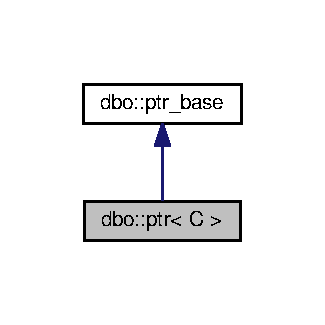
\includegraphics[width=156pt]{classdbo_1_1ptr__inherit__graph}
\end{center}
\end{figure}


Collaboration diagram for dbo\+:\+:ptr$<$ C $>$\+:\nopagebreak
\begin{figure}[H]
\begin{center}
\leavevmode
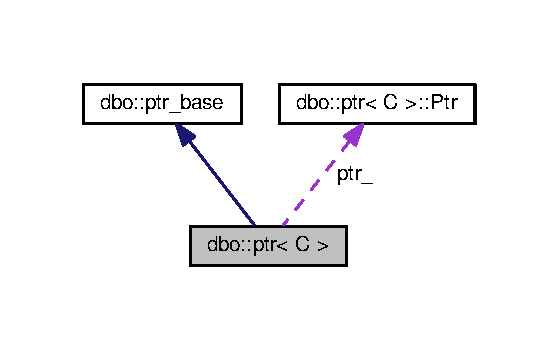
\includegraphics[width=268pt]{classdbo_1_1ptr__coll__graph}
\end{center}
\end{figure}
\subsection*{Classes}
\begin{DoxyCompactItemize}
\item 
struct \hyperlink{structdbo_1_1ptr_1_1_ptr}{Ptr}
\end{DoxyCompactItemize}
\subsection*{Public Types}
\begin{DoxyCompactItemize}
\item 
using \hyperlink{classdbo_1_1ptr_a01fdb2e2c0743eb8bd1b822ccc8d4cd4}{Id\+Type} = typename \hyperlink{structdbo_1_1traits_1_1dbo__traits}{traits\+::dbo\+\_\+traits}$<$ C $>$\+::\hyperlink{classdbo_1_1ptr_a01fdb2e2c0743eb8bd1b822ccc8d4cd4}{Id\+Type}
\end{DoxyCompactItemize}
\subsection*{Public Member Functions}
\begin{DoxyCompactItemize}
\item 
\hyperlink{classdbo_1_1ptr_a3424e8d87ed87f97199e60d72d880222}{ptr} ()
\item 
\hyperlink{classdbo_1_1ptr_a2f545e2c6ac1854ea03d4701e41ea40a}{ptr} (C $\ast$obj)
\item 
\hyperlink{classdbo_1_1ptr_a1bb066cffcb5faaeec23a8e4ab2ef18e}{ptr} (const \hyperlink{classdbo_1_1ptr}{ptr}$<$ C $>$ \&other)
\begin{DoxyCompactList}\small\item\em Copy constructor. \end{DoxyCompactList}\item 
{\footnotesize template$<$class D $>$ }\\\hyperlink{classdbo_1_1ptr_adb1070e230529bd36aa1b262d68960ec}{ptr} (const \hyperlink{classdbo_1_1ptr}{ptr}$<$ D $>$ \&other)
\item 
virtual \hyperlink{classdbo_1_1ptr_ac98aace150c4d051e6bd8354210296f5}{$\sim$ptr} ()
\item 
void \hyperlink{classdbo_1_1ptr_ae4b0ee2c40996915d77d9fcdcc057fb8}{reset} (C $\ast$obj=nullptr)
\begin{DoxyCompactList}\small\item\em Resets the pointer. \end{DoxyCompactList}\item 
\hyperlink{classdbo_1_1ptr}{ptr}$<$ C $>$ \& \hyperlink{classdbo_1_1ptr_a5056e13628f91e9449dd1bd24a761a31}{operator=} (const \hyperlink{classdbo_1_1ptr}{ptr}$<$ C $>$ \&other)
\begin{DoxyCompactList}\small\item\em Assignment operator. \end{DoxyCompactList}\item 
{\footnotesize template$<$class D $>$ }\\\hyperlink{classdbo_1_1ptr}{ptr}$<$ C $>$ \& \hyperlink{classdbo_1_1ptr_a5391736647ac3d24efaad019805b42ca}{operator=} (const \hyperlink{classdbo_1_1ptr}{ptr}$<$ D $>$ \&other)
\item 
C $\ast$ \hyperlink{classdbo_1_1ptr_a19988f39645add72eed820fc754d78bb}{operator-\/$>$} () const 
\begin{DoxyCompactList}\small\item\em Dereference operator. \end{DoxyCompactList}\item 
C $\ast$ \hyperlink{classdbo_1_1ptr_ae05d3e079bd72edd92cb39d218ae6f7b}{get} () const 
\begin{DoxyCompactList}\small\item\em Returns the pointer. \end{DoxyCompactList}\item 
C \& \hyperlink{classdbo_1_1ptr_a5b61379bd3cc91221dd430b24a5cee01}{operator$\ast$} () const 
\begin{DoxyCompactList}\small\item\em Dereference operator. \end{DoxyCompactList}\item 
bool \hyperlink{classdbo_1_1ptr_a733dd776fa6437df42d43c658e9e2b46}{operator==} (const \hyperlink{classdbo_1_1ptr}{ptr}$<$ Mut\+C $>$ \&other) const 
\begin{DoxyCompactList}\small\item\em Comparison operator. \end{DoxyCompactList}\item 
bool \hyperlink{classdbo_1_1ptr_a53ffbe1fc2ff280ec1e51f07340afa59}{operator==} (const \hyperlink{classdbo_1_1ptr}{ptr}$<$ const C $>$ \&other) const 
\item 
bool \hyperlink{classdbo_1_1ptr_aeffa0731ad6db791543528ffc35b06ff}{operator!=} (const \hyperlink{classdbo_1_1ptr}{ptr}$<$ Mut\+C $>$ \&other) const 
\begin{DoxyCompactList}\small\item\em Comparison operator. \end{DoxyCompactList}\item 
bool \hyperlink{classdbo_1_1ptr_a8f75218dcf7602016bd05204de07bd1d}{operator!=} (const \hyperlink{classdbo_1_1ptr}{ptr}$<$ const C $>$ \&other) const 
\item 
bool \hyperlink{classdbo_1_1ptr_a352eff12b264f96f7fb9d8b99490ed0f}{operator$<$} (const \hyperlink{classdbo_1_1ptr}{ptr}$<$ Mut\+C $>$ \&other) const 
\begin{DoxyCompactList}\small\item\em Comparison operator. \end{DoxyCompactList}\item 
bool \hyperlink{classdbo_1_1ptr_a313ecb8531dcac45969342d26da9e0d9}{operator$<$} (const \hyperlink{classdbo_1_1ptr}{ptr}$<$ const C $>$ \&other) const 
\item 
\hyperlink{classdbo_1_1ptr_a72f14c0fec82d1a42ea26d978abaf16e}{operator bool} () const 
\begin{DoxyCompactList}\small\item\em Checks for null. \end{DoxyCompactList}\item 
bool \hyperlink{classdbo_1_1ptr_ab78eab684add44b9fcf6707b562fbf99}{loaded} () const 
\item 
bool \hyperlink{classdbo_1_1ptr_a838311b9897fad3559624d5d83b693a1}{orphan} () const 
\item 
const \hyperlink{classdbo_1_1ptr_a01fdb2e2c0743eb8bd1b822ccc8d4cd4}{Id\+Type} \& \hyperlink{classdbo_1_1ptr_a4de5c28173ca5ade1f7d4a8477d15c0f}{id} () const 
\end{DoxyCompactItemize}
\subsection*{Protected Member Functions}
\begin{DoxyCompactItemize}
\item 
\hyperlink{classdbo_1_1ptr_aaf763715686e40657a744d123b6fd9f8}{ptr} (\hyperlink{structdbo_1_1ptr_1_1_ptr}{Ptr} $\ast$\hyperlink{classdbo_1_1ptr}{ptr})
\item 
void \hyperlink{classdbo_1_1ptr_a792c1c28c473022d02e44c7ce9cfea6c}{free} ()
\item 
void \hyperlink{classdbo_1_1ptr_a0bcf503ebd97de9f203d884d24265789}{take} ()
\item 
void \hyperlink{classdbo_1_1ptr_a36439c82039e32a37fd149d8c54f7ee0}{id} (const \hyperlink{classdbo_1_1ptr_a01fdb2e2c0743eb8bd1b822ccc8d4cd4}{Id\+Type} \&value)
\item 
void \hyperlink{classdbo_1_1ptr_ace8682a6aa620ddb5b664f19cbb63af8}{table\+Name} (const char $\ast$table\+Name)
\end{DoxyCompactItemize}
\subsection*{Protected Attributes}
\begin{DoxyCompactItemize}
\item 
char $\ast$ \hyperlink{classdbo_1_1ptr_aa021e5c70d53414dfbb3139ce3661b9d}{table\+Name\+\_\+}
\item 
\hyperlink{structdbo_1_1ptr_1_1_ptr}{Ptr} $\ast$ \hyperlink{classdbo_1_1ptr_a7c58e1f0ae8dcf8a7a9acd6197d2de38}{ptr\+\_\+}
\end{DoxyCompactItemize}
\subsection*{Static Protected Attributes}
\begin{DoxyCompactItemize}
\item 
static \hyperlink{classdbo_1_1ptr_a01fdb2e2c0743eb8bd1b822ccc8d4cd4}{Id\+Type} \hyperlink{classdbo_1_1ptr_a26f06bd10de2444190c904a1814999fa}{invalid\+Id\+\_\+} =\hyperlink{structdbo_1_1traits_1_1dbo__traits}{traits\+::dbo\+\_\+traits}$<$C$>$\+::invalid\+Id()
\end{DoxyCompactItemize}
\subsection*{Friends}
\begin{DoxyCompactItemize}
\item 
class \hyperlink{classdbo_1_1ptr_adb115488bb4890f7fc705ee527ad71e0}{connection}
\item 
{\footnotesize template$<$class T $>$ }\\class \hyperlink{classdbo_1_1ptr_ae779179e16547c9a93329dd197385493}{action\+::\+Delete}
\item 
{\footnotesize template$<$class T $>$ }\\class \hyperlink{classdbo_1_1ptr_a88a9b73e2cb3304941371508b660e53e}{action\+::\+Insert}
\item 
{\footnotesize template$<$class T $>$ }\\class \hyperlink{classdbo_1_1ptr_a90af99826aea472a0aa22e59376fed0f}{action\+::\+Update}
\item 
{\footnotesize template$<$class T $>$ }\\class \hyperlink{classdbo_1_1ptr_a8b98481706995f8b3e2665f74b2b3039}{action\+::\+Select\+By\+Id}
\item 
class \hyperlink{classdbo_1_1ptr_a7fddf73eaed86e45a2aacbd26b5af751}{query}
\item 
{\footnotesize template$<$class D $>$ }\\class \hyperlink{classdbo_1_1ptr_a916ea84dc420573cfdb360b67445d5d0}{collection}
\item 
std\+::ostream \& \hyperlink{classdbo_1_1ptr_a70a1cd538b5f03fbc42965ac8f918f23}{operator$<$$<$} (std\+::ostream \&o, const \hyperlink{classdbo_1_1ptr}{ptr}$<$ C $>$ \&\+\_\+ptr)
\end{DoxyCompactItemize}


\subsection{Member Typedef Documentation}
\hypertarget{classdbo_1_1ptr_a01fdb2e2c0743eb8bd1b822ccc8d4cd4}{\index{dbo\+::ptr@{dbo\+::ptr}!Id\+Type@{Id\+Type}}
\index{Id\+Type@{Id\+Type}!dbo\+::ptr@{dbo\+::ptr}}
\subsubsection[{Id\+Type}]{\setlength{\rightskip}{0pt plus 5cm}template$<$class C$>$ using {\bf dbo\+::ptr}$<$ C $>$\+::{\bf Id\+Type} =  typename {\bf traits\+::dbo\+\_\+traits}$<$C$>$\+::{\bf Id\+Type}}}\label{classdbo_1_1ptr_a01fdb2e2c0743eb8bd1b822ccc8d4cd4}


\subsection{Constructor \& Destructor Documentation}
\hypertarget{classdbo_1_1ptr_a3424e8d87ed87f97199e60d72d880222}{\index{dbo\+::ptr@{dbo\+::ptr}!ptr@{ptr}}
\index{ptr@{ptr}!dbo\+::ptr@{dbo\+::ptr}}
\subsubsection[{ptr}]{\setlength{\rightskip}{0pt plus 5cm}template$<$class C $>$ {\bf dbo\+::ptr}$<$ C $>$\+::{\bf ptr} (
\begin{DoxyParamCaption}
{}
\end{DoxyParamCaption}
)}}\label{classdbo_1_1ptr_a3424e8d87ed87f97199e60d72d880222}
\hypertarget{classdbo_1_1ptr_a2f545e2c6ac1854ea03d4701e41ea40a}{\index{dbo\+::ptr@{dbo\+::ptr}!ptr@{ptr}}
\index{ptr@{ptr}!dbo\+::ptr@{dbo\+::ptr}}
\subsubsection[{ptr}]{\setlength{\rightskip}{0pt plus 5cm}template$<$class C $>$ {\bf dbo\+::ptr}$<$ C $>$\+::{\bf ptr} (
\begin{DoxyParamCaption}
\item[{C $\ast$}]{obj}
\end{DoxyParamCaption}
)}}\label{classdbo_1_1ptr_a2f545e2c6ac1854ea03d4701e41ea40a}
\hypertarget{classdbo_1_1ptr_a1bb066cffcb5faaeec23a8e4ab2ef18e}{\index{dbo\+::ptr@{dbo\+::ptr}!ptr@{ptr}}
\index{ptr@{ptr}!dbo\+::ptr@{dbo\+::ptr}}
\subsubsection[{ptr}]{\setlength{\rightskip}{0pt plus 5cm}template$<$class C $>$ {\bf dbo\+::ptr}$<$ C $>$\+::{\bf ptr} (
\begin{DoxyParamCaption}
\item[{const {\bf ptr}$<$ C $>$ \&}]{other}
\end{DoxyParamCaption}
)}}\label{classdbo_1_1ptr_a1bb066cffcb5faaeec23a8e4ab2ef18e}


Copy constructor. 

\hypertarget{classdbo_1_1ptr_adb1070e230529bd36aa1b262d68960ec}{\index{dbo\+::ptr@{dbo\+::ptr}!ptr@{ptr}}
\index{ptr@{ptr}!dbo\+::ptr@{dbo\+::ptr}}
\subsubsection[{ptr}]{\setlength{\rightskip}{0pt plus 5cm}template$<$class C $>$ template$<$class D $>$ {\bf dbo\+::ptr}$<$ C $>$\+::{\bf ptr} (
\begin{DoxyParamCaption}
\item[{const {\bf ptr}$<$ D $>$ \&}]{other}
\end{DoxyParamCaption}
)}}\label{classdbo_1_1ptr_adb1070e230529bd36aa1b262d68960ec}
\hypertarget{classdbo_1_1ptr_ac98aace150c4d051e6bd8354210296f5}{\index{dbo\+::ptr@{dbo\+::ptr}!````~ptr@{$\sim$ptr}}
\index{````~ptr@{$\sim$ptr}!dbo\+::ptr@{dbo\+::ptr}}
\subsubsection[{$\sim$ptr}]{\setlength{\rightskip}{0pt plus 5cm}template$<$class C $>$ {\bf dbo\+::ptr}$<$ C $>$\+::$\sim${\bf ptr} (
\begin{DoxyParamCaption}
{}
\end{DoxyParamCaption}
)\hspace{0.3cm}{\ttfamily [virtual]}}}\label{classdbo_1_1ptr_ac98aace150c4d051e6bd8354210296f5}
\hypertarget{classdbo_1_1ptr_aaf763715686e40657a744d123b6fd9f8}{\index{dbo\+::ptr@{dbo\+::ptr}!ptr@{ptr}}
\index{ptr@{ptr}!dbo\+::ptr@{dbo\+::ptr}}
\subsubsection[{ptr}]{\setlength{\rightskip}{0pt plus 5cm}template$<$class C $>$ {\bf dbo\+::ptr}$<$ C $>$\+::{\bf ptr} (
\begin{DoxyParamCaption}
\item[{{\bf Ptr} $\ast$}]{ptr}
\end{DoxyParamCaption}
)\hspace{0.3cm}{\ttfamily [protected]}}}\label{classdbo_1_1ptr_aaf763715686e40657a744d123b6fd9f8}


\subsection{Member Function Documentation}
\hypertarget{classdbo_1_1ptr_a792c1c28c473022d02e44c7ce9cfea6c}{\index{dbo\+::ptr@{dbo\+::ptr}!free@{free}}
\index{free@{free}!dbo\+::ptr@{dbo\+::ptr}}
\subsubsection[{free}]{\setlength{\rightskip}{0pt plus 5cm}template$<$class C $>$ void {\bf dbo\+::ptr}$<$ C $>$\+::free (
\begin{DoxyParamCaption}
{}
\end{DoxyParamCaption}
)\hspace{0.3cm}{\ttfamily [protected]}}}\label{classdbo_1_1ptr_a792c1c28c473022d02e44c7ce9cfea6c}
\hypertarget{classdbo_1_1ptr_ae05d3e079bd72edd92cb39d218ae6f7b}{\index{dbo\+::ptr@{dbo\+::ptr}!get@{get}}
\index{get@{get}!dbo\+::ptr@{dbo\+::ptr}}
\subsubsection[{get}]{\setlength{\rightskip}{0pt plus 5cm}template$<$class C $>$ C $\ast$ {\bf dbo\+::ptr}$<$ C $>$\+::get (
\begin{DoxyParamCaption}
{}
\end{DoxyParamCaption}
) const}}\label{classdbo_1_1ptr_ae05d3e079bd72edd92cb39d218ae6f7b}


Returns the pointer. 

Note that returns a const pointer. Use modify() to get a non-\/const pointer.

Since this may lazy-\/load the underlying database object, you should have an active transaction.

\begin{DoxySeeAlso}{See also}
modify() 
\end{DoxySeeAlso}
\hypertarget{classdbo_1_1ptr_a4de5c28173ca5ade1f7d4a8477d15c0f}{\index{dbo\+::ptr@{dbo\+::ptr}!id@{id}}
\index{id@{id}!dbo\+::ptr@{dbo\+::ptr}}
\subsubsection[{id}]{\setlength{\rightskip}{0pt plus 5cm}template$<$class C $>$ const {\bf ptr}$<$ C $>$\+::{\bf Id\+Type} \& {\bf dbo\+::ptr}$<$ C $>$\+::id (
\begin{DoxyParamCaption}
{}
\end{DoxyParamCaption}
) const}}\label{classdbo_1_1ptr_a4de5c28173ca5ade1f7d4a8477d15c0f}
\hypertarget{classdbo_1_1ptr_a36439c82039e32a37fd149d8c54f7ee0}{\index{dbo\+::ptr@{dbo\+::ptr}!id@{id}}
\index{id@{id}!dbo\+::ptr@{dbo\+::ptr}}
\subsubsection[{id}]{\setlength{\rightskip}{0pt plus 5cm}template$<$class C$>$ void {\bf dbo\+::ptr}$<$ C $>$\+::id (
\begin{DoxyParamCaption}
\item[{const {\bf Id\+Type} \&}]{value}
\end{DoxyParamCaption}
)\hspace{0.3cm}{\ttfamily [protected]}}}\label{classdbo_1_1ptr_a36439c82039e32a37fd149d8c54f7ee0}
\hypertarget{classdbo_1_1ptr_ab78eab684add44b9fcf6707b562fbf99}{\index{dbo\+::ptr@{dbo\+::ptr}!loaded@{loaded}}
\index{loaded@{loaded}!dbo\+::ptr@{dbo\+::ptr}}
\subsubsection[{loaded}]{\setlength{\rightskip}{0pt plus 5cm}template$<$class C $>$ bool {\bf dbo\+::ptr}$<$ C $>$\+::loaded (
\begin{DoxyParamCaption}
{}
\end{DoxyParamCaption}
) const}}\label{classdbo_1_1ptr_ab78eab684add44b9fcf6707b562fbf99}
An object is considered as loaded if it has a content and a valid id \hypertarget{classdbo_1_1ptr_a72f14c0fec82d1a42ea26d978abaf16e}{\index{dbo\+::ptr@{dbo\+::ptr}!operator bool@{operator bool}}
\index{operator bool@{operator bool}!dbo\+::ptr@{dbo\+::ptr}}
\subsubsection[{operator bool}]{\setlength{\rightskip}{0pt plus 5cm}template$<$class C $>$ {\bf dbo\+::ptr}$<$ C $>$\+::operator bool (
\begin{DoxyParamCaption}
{}
\end{DoxyParamCaption}
) const\hspace{0.3cm}{\ttfamily [explicit]}}}\label{classdbo_1_1ptr_a72f14c0fec82d1a42ea26d978abaf16e}


Checks for null. 

Returns true if the pointer is pointing to a non-\/null object. \hypertarget{classdbo_1_1ptr_aeffa0731ad6db791543528ffc35b06ff}{\index{dbo\+::ptr@{dbo\+::ptr}!operator"!=@{operator"!=}}
\index{operator"!=@{operator"!=}!dbo\+::ptr@{dbo\+::ptr}}
\subsubsection[{operator"!=}]{\setlength{\rightskip}{0pt plus 5cm}template$<$class C $>$ bool {\bf dbo\+::ptr}$<$ C $>$\+::operator!= (
\begin{DoxyParamCaption}
\item[{const {\bf ptr}$<$ Mut\+C $>$ \&}]{other}
\end{DoxyParamCaption}
) const}}\label{classdbo_1_1ptr_aeffa0731ad6db791543528ffc35b06ff}


Comparison operator. 

Two pointers are equal if and only if they reference the same database object. \hypertarget{classdbo_1_1ptr_a8f75218dcf7602016bd05204de07bd1d}{\index{dbo\+::ptr@{dbo\+::ptr}!operator"!=@{operator"!=}}
\index{operator"!=@{operator"!=}!dbo\+::ptr@{dbo\+::ptr}}
\subsubsection[{operator"!=}]{\setlength{\rightskip}{0pt plus 5cm}template$<$class C $>$ bool {\bf dbo\+::ptr}$<$ C $>$\+::operator!= (
\begin{DoxyParamCaption}
\item[{const {\bf ptr}$<$ const C $>$ \&}]{other}
\end{DoxyParamCaption}
) const}}\label{classdbo_1_1ptr_a8f75218dcf7602016bd05204de07bd1d}
\hypertarget{classdbo_1_1ptr_a5b61379bd3cc91221dd430b24a5cee01}{\index{dbo\+::ptr@{dbo\+::ptr}!operator$\ast$@{operator$\ast$}}
\index{operator$\ast$@{operator$\ast$}!dbo\+::ptr@{dbo\+::ptr}}
\subsubsection[{operator$\ast$}]{\setlength{\rightskip}{0pt plus 5cm}template$<$class C $>$ C \& {\bf dbo\+::ptr}$<$ C $>$\+::operator$\ast$ (
\begin{DoxyParamCaption}
{}
\end{DoxyParamCaption}
) const}}\label{classdbo_1_1ptr_a5b61379bd3cc91221dd430b24a5cee01}


Dereference operator. 

Note that this operator returns a const copy of the referenced object. Use modify() to get a non-\/const reference.

Since this may lazy-\/load the underlying database object, you should have an active transaction. \hypertarget{classdbo_1_1ptr_a19988f39645add72eed820fc754d78bb}{\index{dbo\+::ptr@{dbo\+::ptr}!operator-\/$>$@{operator-\/$>$}}
\index{operator-\/$>$@{operator-\/$>$}!dbo\+::ptr@{dbo\+::ptr}}
\subsubsection[{operator-\/$>$}]{\setlength{\rightskip}{0pt plus 5cm}template$<$class C $>$ C $\ast$ {\bf dbo\+::ptr}$<$ C $>$\+::operator-\/$>$ (
\begin{DoxyParamCaption}
{}
\end{DoxyParamCaption}
) const}}\label{classdbo_1_1ptr_a19988f39645add72eed820fc754d78bb}


Dereference operator. 

Note that this operator returns a const copy of the referenced object. Use modify() to get a non-\/const reference.

Since this may lazy-\/load the underlying database object, you should have an active transaction. \hypertarget{classdbo_1_1ptr_a352eff12b264f96f7fb9d8b99490ed0f}{\index{dbo\+::ptr@{dbo\+::ptr}!operator$<$@{operator$<$}}
\index{operator$<$@{operator$<$}!dbo\+::ptr@{dbo\+::ptr}}
\subsubsection[{operator$<$}]{\setlength{\rightskip}{0pt plus 5cm}template$<$class C $>$ bool {\bf dbo\+::ptr}$<$ C $>$\+::operator$<$ (
\begin{DoxyParamCaption}
\item[{const {\bf ptr}$<$ Mut\+C $>$ \&}]{other}
\end{DoxyParamCaption}
) const}}\label{classdbo_1_1ptr_a352eff12b264f96f7fb9d8b99490ed0f}


Comparison operator. 

This operator is implemented to be able to store pointers in std\+::set or std\+::map containers. \hypertarget{classdbo_1_1ptr_a313ecb8531dcac45969342d26da9e0d9}{\index{dbo\+::ptr@{dbo\+::ptr}!operator$<$@{operator$<$}}
\index{operator$<$@{operator$<$}!dbo\+::ptr@{dbo\+::ptr}}
\subsubsection[{operator$<$}]{\setlength{\rightskip}{0pt plus 5cm}template$<$class C $>$ bool {\bf dbo\+::ptr}$<$ C $>$\+::operator$<$ (
\begin{DoxyParamCaption}
\item[{const {\bf ptr}$<$ const C $>$ \&}]{other}
\end{DoxyParamCaption}
) const}}\label{classdbo_1_1ptr_a313ecb8531dcac45969342d26da9e0d9}
\hypertarget{classdbo_1_1ptr_a5056e13628f91e9449dd1bd24a761a31}{\index{dbo\+::ptr@{dbo\+::ptr}!operator=@{operator=}}
\index{operator=@{operator=}!dbo\+::ptr@{dbo\+::ptr}}
\subsubsection[{operator=}]{\setlength{\rightskip}{0pt plus 5cm}template$<$class C $>$ {\bf ptr}$<$ C $>$ \& {\bf dbo\+::ptr}$<$ C $>$\+::operator= (
\begin{DoxyParamCaption}
\item[{const {\bf ptr}$<$ C $>$ \&}]{other}
\end{DoxyParamCaption}
)}}\label{classdbo_1_1ptr_a5056e13628f91e9449dd1bd24a761a31}


Assignment operator. 

\hypertarget{classdbo_1_1ptr_a5391736647ac3d24efaad019805b42ca}{\index{dbo\+::ptr@{dbo\+::ptr}!operator=@{operator=}}
\index{operator=@{operator=}!dbo\+::ptr@{dbo\+::ptr}}
\subsubsection[{operator=}]{\setlength{\rightskip}{0pt plus 5cm}template$<$class C $>$ template$<$class D $>$ {\bf ptr}$<$ C $>$ \& {\bf dbo\+::ptr}$<$ C $>$\+::operator= (
\begin{DoxyParamCaption}
\item[{const {\bf ptr}$<$ D $>$ \&}]{other}
\end{DoxyParamCaption}
)}}\label{classdbo_1_1ptr_a5391736647ac3d24efaad019805b42ca}
\hypertarget{classdbo_1_1ptr_a733dd776fa6437df42d43c658e9e2b46}{\index{dbo\+::ptr@{dbo\+::ptr}!operator==@{operator==}}
\index{operator==@{operator==}!dbo\+::ptr@{dbo\+::ptr}}
\subsubsection[{operator==}]{\setlength{\rightskip}{0pt plus 5cm}template$<$class C $>$ bool {\bf dbo\+::ptr}$<$ C $>$\+::operator== (
\begin{DoxyParamCaption}
\item[{const {\bf ptr}$<$ Mut\+C $>$ \&}]{other}
\end{DoxyParamCaption}
) const}}\label{classdbo_1_1ptr_a733dd776fa6437df42d43c658e9e2b46}


Comparison operator. 

Two pointers are equal if and only if they reference the same database object. \hypertarget{classdbo_1_1ptr_a53ffbe1fc2ff280ec1e51f07340afa59}{\index{dbo\+::ptr@{dbo\+::ptr}!operator==@{operator==}}
\index{operator==@{operator==}!dbo\+::ptr@{dbo\+::ptr}}
\subsubsection[{operator==}]{\setlength{\rightskip}{0pt plus 5cm}template$<$class C $>$ bool {\bf dbo\+::ptr}$<$ C $>$\+::operator== (
\begin{DoxyParamCaption}
\item[{const {\bf ptr}$<$ const C $>$ \&}]{other}
\end{DoxyParamCaption}
) const}}\label{classdbo_1_1ptr_a53ffbe1fc2ff280ec1e51f07340afa59}
\hypertarget{classdbo_1_1ptr_a838311b9897fad3559624d5d83b693a1}{\index{dbo\+::ptr@{dbo\+::ptr}!orphan@{orphan}}
\index{orphan@{orphan}!dbo\+::ptr@{dbo\+::ptr}}
\subsubsection[{orphan}]{\setlength{\rightskip}{0pt plus 5cm}template$<$class C $>$ bool {\bf dbo\+::ptr}$<$ C $>$\+::orphan (
\begin{DoxyParamCaption}
{}
\end{DoxyParamCaption}
) const}}\label{classdbo_1_1ptr_a838311b9897fad3559624d5d83b693a1}
An object is considered as orphaned if it has a content and an invalid id \hypertarget{classdbo_1_1ptr_ae4b0ee2c40996915d77d9fcdcc057fb8}{\index{dbo\+::ptr@{dbo\+::ptr}!reset@{reset}}
\index{reset@{reset}!dbo\+::ptr@{dbo\+::ptr}}
\subsubsection[{reset}]{\setlength{\rightskip}{0pt plus 5cm}template$<$class C $>$ void {\bf dbo\+::ptr}$<$ C $>$\+::reset (
\begin{DoxyParamCaption}
\item[{C $\ast$}]{obj = {\ttfamily nullptr$<$~C~$>$}}
\end{DoxyParamCaption}
)}}\label{classdbo_1_1ptr_ae4b0ee2c40996915d77d9fcdcc057fb8}


Resets the pointer. 

This is equivalent to\+: 
\begin{DoxyCode}
p = ptr<C>(obj);
\end{DoxyCode}
 \hypertarget{classdbo_1_1ptr_ace8682a6aa620ddb5b664f19cbb63af8}{\index{dbo\+::ptr@{dbo\+::ptr}!table\+Name@{table\+Name}}
\index{table\+Name@{table\+Name}!dbo\+::ptr@{dbo\+::ptr}}
\subsubsection[{table\+Name}]{\setlength{\rightskip}{0pt plus 5cm}template$<$class C $>$ void {\bf dbo\+::ptr}$<$ C $>$\+::table\+Name (
\begin{DoxyParamCaption}
\item[{const char $\ast$}]{table\+Name}
\end{DoxyParamCaption}
)\hspace{0.3cm}{\ttfamily [protected]}}}\label{classdbo_1_1ptr_ace8682a6aa620ddb5b664f19cbb63af8}
\hypertarget{classdbo_1_1ptr_a0bcf503ebd97de9f203d884d24265789}{\index{dbo\+::ptr@{dbo\+::ptr}!take@{take}}
\index{take@{take}!dbo\+::ptr@{dbo\+::ptr}}
\subsubsection[{take}]{\setlength{\rightskip}{0pt plus 5cm}template$<$class C $>$ void {\bf dbo\+::ptr}$<$ C $>$\+::take (
\begin{DoxyParamCaption}
{}
\end{DoxyParamCaption}
)\hspace{0.3cm}{\ttfamily [protected]}}}\label{classdbo_1_1ptr_a0bcf503ebd97de9f203d884d24265789}


\subsection{Friends And Related Function Documentation}
\hypertarget{classdbo_1_1ptr_ae779179e16547c9a93329dd197385493}{\index{dbo\+::ptr@{dbo\+::ptr}!action\+::\+Delete@{action\+::\+Delete}}
\index{action\+::\+Delete@{action\+::\+Delete}!dbo\+::ptr@{dbo\+::ptr}}
\subsubsection[{action\+::\+Delete}]{\setlength{\rightskip}{0pt plus 5cm}template$<$class C$>$ template$<$class T $>$ friend class {\bf action\+::\+Delete}\hspace{0.3cm}{\ttfamily [friend]}}}\label{classdbo_1_1ptr_ae779179e16547c9a93329dd197385493}
\hypertarget{classdbo_1_1ptr_a88a9b73e2cb3304941371508b660e53e}{\index{dbo\+::ptr@{dbo\+::ptr}!action\+::\+Insert@{action\+::\+Insert}}
\index{action\+::\+Insert@{action\+::\+Insert}!dbo\+::ptr@{dbo\+::ptr}}
\subsubsection[{action\+::\+Insert}]{\setlength{\rightskip}{0pt plus 5cm}template$<$class C$>$ template$<$class T $>$ friend class {\bf action\+::\+Insert}\hspace{0.3cm}{\ttfamily [friend]}}}\label{classdbo_1_1ptr_a88a9b73e2cb3304941371508b660e53e}
\hypertarget{classdbo_1_1ptr_a8b98481706995f8b3e2665f74b2b3039}{\index{dbo\+::ptr@{dbo\+::ptr}!action\+::\+Select\+By\+Id@{action\+::\+Select\+By\+Id}}
\index{action\+::\+Select\+By\+Id@{action\+::\+Select\+By\+Id}!dbo\+::ptr@{dbo\+::ptr}}
\subsubsection[{action\+::\+Select\+By\+Id}]{\setlength{\rightskip}{0pt plus 5cm}template$<$class C$>$ template$<$class T $>$ friend class {\bf action\+::\+Select\+By\+Id}\hspace{0.3cm}{\ttfamily [friend]}}}\label{classdbo_1_1ptr_a8b98481706995f8b3e2665f74b2b3039}
\hypertarget{classdbo_1_1ptr_a90af99826aea472a0aa22e59376fed0f}{\index{dbo\+::ptr@{dbo\+::ptr}!action\+::\+Update@{action\+::\+Update}}
\index{action\+::\+Update@{action\+::\+Update}!dbo\+::ptr@{dbo\+::ptr}}
\subsubsection[{action\+::\+Update}]{\setlength{\rightskip}{0pt plus 5cm}template$<$class C$>$ template$<$class T $>$ friend class {\bf action\+::\+Update}\hspace{0.3cm}{\ttfamily [friend]}}}\label{classdbo_1_1ptr_a90af99826aea472a0aa22e59376fed0f}
\hypertarget{classdbo_1_1ptr_a916ea84dc420573cfdb360b67445d5d0}{\index{dbo\+::ptr@{dbo\+::ptr}!collection@{collection}}
\index{collection@{collection}!dbo\+::ptr@{dbo\+::ptr}}
\subsubsection[{collection}]{\setlength{\rightskip}{0pt plus 5cm}template$<$class C$>$ template$<$class D $>$ friend class {\bf collection}\hspace{0.3cm}{\ttfamily [friend]}}}\label{classdbo_1_1ptr_a916ea84dc420573cfdb360b67445d5d0}
\hypertarget{classdbo_1_1ptr_adb115488bb4890f7fc705ee527ad71e0}{\index{dbo\+::ptr@{dbo\+::ptr}!connection@{connection}}
\index{connection@{connection}!dbo\+::ptr@{dbo\+::ptr}}
\subsubsection[{connection}]{\setlength{\rightskip}{0pt plus 5cm}template$<$class C$>$ friend class {\bf connection}\hspace{0.3cm}{\ttfamily [friend]}}}\label{classdbo_1_1ptr_adb115488bb4890f7fc705ee527ad71e0}
\hypertarget{classdbo_1_1ptr_a70a1cd538b5f03fbc42965ac8f918f23}{\index{dbo\+::ptr@{dbo\+::ptr}!operator$<$$<$@{operator$<$$<$}}
\index{operator$<$$<$@{operator$<$$<$}!dbo\+::ptr@{dbo\+::ptr}}
\subsubsection[{operator$<$$<$}]{\setlength{\rightskip}{0pt plus 5cm}template$<$class C$>$ std\+::ostream\& operator$<$$<$ (
\begin{DoxyParamCaption}
\item[{std\+::ostream \&}]{o, }
\item[{const {\bf ptr}$<$ C $>$ \&}]{\+\_\+ptr}
\end{DoxyParamCaption}
)\hspace{0.3cm}{\ttfamily [friend]}}}\label{classdbo_1_1ptr_a70a1cd538b5f03fbc42965ac8f918f23}
\hypertarget{classdbo_1_1ptr_a7fddf73eaed86e45a2aacbd26b5af751}{\index{dbo\+::ptr@{dbo\+::ptr}!query@{query}}
\index{query@{query}!dbo\+::ptr@{dbo\+::ptr}}
\subsubsection[{query}]{\setlength{\rightskip}{0pt plus 5cm}template$<$class C$>$ friend class {\bf query}\hspace{0.3cm}{\ttfamily [friend]}}}\label{classdbo_1_1ptr_a7fddf73eaed86e45a2aacbd26b5af751}


\subsection{Member Data Documentation}
\hypertarget{classdbo_1_1ptr_a26f06bd10de2444190c904a1814999fa}{\index{dbo\+::ptr@{dbo\+::ptr}!invalid\+Id\+\_\+@{invalid\+Id\+\_\+}}
\index{invalid\+Id\+\_\+@{invalid\+Id\+\_\+}!dbo\+::ptr@{dbo\+::ptr}}
\subsubsection[{invalid\+Id\+\_\+}]{\setlength{\rightskip}{0pt plus 5cm}template$<$class C$>$ {\bf ptr}$<$ C $>$\+::{\bf Id\+Type} {\bf dbo\+::ptr}$<$ C $>$\+::invalid\+Id\+\_\+ ={\bf traits\+::dbo\+\_\+traits}$<$C$>$\+::invalid\+Id()\hspace{0.3cm}{\ttfamily [static]}, {\ttfamily [protected]}}}\label{classdbo_1_1ptr_a26f06bd10de2444190c904a1814999fa}
\hypertarget{classdbo_1_1ptr_a7c58e1f0ae8dcf8a7a9acd6197d2de38}{\index{dbo\+::ptr@{dbo\+::ptr}!ptr\+\_\+@{ptr\+\_\+}}
\index{ptr\+\_\+@{ptr\+\_\+}!dbo\+::ptr@{dbo\+::ptr}}
\subsubsection[{ptr\+\_\+}]{\setlength{\rightskip}{0pt plus 5cm}template$<$class C$>$ {\bf Ptr}$\ast$ {\bf dbo\+::ptr}$<$ C $>$\+::ptr\+\_\+\hspace{0.3cm}{\ttfamily [protected]}}}\label{classdbo_1_1ptr_a7c58e1f0ae8dcf8a7a9acd6197d2de38}
\hypertarget{classdbo_1_1ptr_aa021e5c70d53414dfbb3139ce3661b9d}{\index{dbo\+::ptr@{dbo\+::ptr}!table\+Name\+\_\+@{table\+Name\+\_\+}}
\index{table\+Name\+\_\+@{table\+Name\+\_\+}!dbo\+::ptr@{dbo\+::ptr}}
\subsubsection[{table\+Name\+\_\+}]{\setlength{\rightskip}{0pt plus 5cm}template$<$class C$>$ char$\ast$ {\bf dbo\+::ptr}$<$ C $>$\+::table\+Name\+\_\+\hspace{0.3cm}{\ttfamily [protected]}}}\label{classdbo_1_1ptr_aa021e5c70d53414dfbb3139ce3661b9d}


The documentation for this class was generated from the following files\+:\begin{DoxyCompactItemize}
\item 
dbo/\hyperlink{collection_8hpp}{collection.\+hpp}\item 
dbo/\hyperlink{ptr_8hpp}{ptr.\+hpp}\item 
dbo/\hyperlink{ptr_8cxx}{ptr.\+cxx}\end{DoxyCompactItemize}

\hypertarget{structdbo_1_1ptr_1_1_ptr}{\section{dbo\+:\+:ptr$<$ C $>$\+:\+:Ptr Struct Reference}
\label{structdbo_1_1ptr_1_1_ptr}\index{dbo\+::ptr$<$ C $>$\+::\+Ptr@{dbo\+::ptr$<$ C $>$\+::\+Ptr}}
}


{\ttfamily \#include $<$ptr.\+hpp$>$}

\subsection*{Public Attributes}
\begin{DoxyCompactItemize}
\item 
C $\ast$ \hyperlink{structdbo_1_1ptr_1_1_ptr_a2c8c1946bb5c45335527e5061114d006}{value\+\_\+}
\item 
size\+\_\+t \hyperlink{structdbo_1_1ptr_1_1_ptr_ae83cda6b6079bc21863c09008b99ef71}{ref\+\_\+}
\item 
\hyperlink{classdbo_1_1ptr_a01fdb2e2c0743eb8bd1b822ccc8d4cd4}{Id\+Type} \hyperlink{structdbo_1_1ptr_1_1_ptr_a2a31f071054839bcbadb7e82ac5f3495}{id\+\_\+}
\end{DoxyCompactItemize}


\subsection{Member Data Documentation}
\hypertarget{structdbo_1_1ptr_1_1_ptr_a2a31f071054839bcbadb7e82ac5f3495}{\index{dbo\+::ptr\+::\+Ptr@{dbo\+::ptr\+::\+Ptr}!id\+\_\+@{id\+\_\+}}
\index{id\+\_\+@{id\+\_\+}!dbo\+::ptr\+::\+Ptr@{dbo\+::ptr\+::\+Ptr}}
\subsubsection[{id\+\_\+}]{\setlength{\rightskip}{0pt plus 5cm}template$<$class C$>$ {\bf Id\+Type} {\bf dbo\+::ptr}$<$ C $>$\+::Ptr\+::id\+\_\+}}\label{structdbo_1_1ptr_1_1_ptr_a2a31f071054839bcbadb7e82ac5f3495}
\hypertarget{structdbo_1_1ptr_1_1_ptr_ae83cda6b6079bc21863c09008b99ef71}{\index{dbo\+::ptr\+::\+Ptr@{dbo\+::ptr\+::\+Ptr}!ref\+\_\+@{ref\+\_\+}}
\index{ref\+\_\+@{ref\+\_\+}!dbo\+::ptr\+::\+Ptr@{dbo\+::ptr\+::\+Ptr}}
\subsubsection[{ref\+\_\+}]{\setlength{\rightskip}{0pt plus 5cm}template$<$class C$>$ size\+\_\+t {\bf dbo\+::ptr}$<$ C $>$\+::Ptr\+::ref\+\_\+}}\label{structdbo_1_1ptr_1_1_ptr_ae83cda6b6079bc21863c09008b99ef71}
\hypertarget{structdbo_1_1ptr_1_1_ptr_a2c8c1946bb5c45335527e5061114d006}{\index{dbo\+::ptr\+::\+Ptr@{dbo\+::ptr\+::\+Ptr}!value\+\_\+@{value\+\_\+}}
\index{value\+\_\+@{value\+\_\+}!dbo\+::ptr\+::\+Ptr@{dbo\+::ptr\+::\+Ptr}}
\subsubsection[{value\+\_\+}]{\setlength{\rightskip}{0pt plus 5cm}template$<$class C$>$ C$\ast$ {\bf dbo\+::ptr}$<$ C $>$\+::Ptr\+::value\+\_\+}}\label{structdbo_1_1ptr_1_1_ptr_a2c8c1946bb5c45335527e5061114d006}


The documentation for this struct was generated from the following file\+:\begin{DoxyCompactItemize}
\item 
dbo/\hyperlink{ptr_8hpp}{ptr.\+hpp}\end{DoxyCompactItemize}

\hypertarget{classdbo_1_1ptr__base}{\section{dbo\+:\+:ptr\+\_\+base Class Reference}
\label{classdbo_1_1ptr__base}\index{dbo\+::ptr\+\_\+base@{dbo\+::ptr\+\_\+base}}
}


{\ttfamily \#include $<$ptr.\+hpp$>$}



Inheritance diagram for dbo\+:\+:ptr\+\_\+base\+:\nopagebreak
\begin{figure}[H]
\begin{center}
\leavevmode
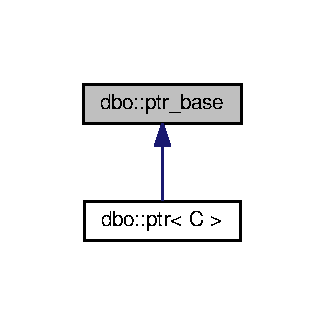
\includegraphics[width=156pt]{classdbo_1_1ptr__base__inherit__graph}
\end{center}
\end{figure}


The documentation for this class was generated from the following file\+:\begin{DoxyCompactItemize}
\item 
dbo/\hyperlink{ptr_8hpp}{ptr.\+hpp}\end{DoxyCompactItemize}

\hypertarget{classdbo_1_1mapping_1_1_ptr_ref}{\section{dbo\+:\+:mapping\+:\+:Ptr\+Ref$<$ T $>$ Class Template Reference}
\label{classdbo_1_1mapping_1_1_ptr_ref}\index{dbo\+::mapping\+::\+Ptr\+Ref$<$ T $>$@{dbo\+::mapping\+::\+Ptr\+Ref$<$ T $>$}}
}


{\ttfamily \#include $<$Bulk\+Insert.\+hpp$>$}

\subsection*{Public Member Functions}
\begin{DoxyCompactItemize}
\item 
\hyperlink{classdbo_1_1mapping_1_1_ptr_ref_a4db1b98f81576daa11f9f1bea49b35bb}{Ptr\+Ref} (\hyperlink{classdbo_1_1ptr}{ptr}$<$ C $>$ \&\hyperlink{classdbo_1_1mapping_1_1_ptr_ref_aa8e1c4fddbf00c5500980afb1f55ade8}{value}, const std\+::string \&\hyperlink{classdbo_1_1mapping_1_1_ptr_ref_a69221246e46fc6a9acb768fe4481cdf3}{name}, int size, int \hyperlink{classdbo_1_1mapping_1_1_ptr_ref_acff9c1f76ec5eca8c092d021bf59b0b0}{fk\+Constraints})
\item 
const std\+::string \& \hyperlink{classdbo_1_1mapping_1_1_ptr_ref_a69221246e46fc6a9acb768fe4481cdf3}{name} () const 
\item 
int \hyperlink{classdbo_1_1mapping_1_1_ptr_ref_acff9c1f76ec5eca8c092d021bf59b0b0}{fk\+Constraints} () const 
\item 
\hyperlink{classdbo_1_1ptr}{ptr}$<$ C $>$ \& \hyperlink{classdbo_1_1mapping_1_1_ptr_ref_aa8e1c4fddbf00c5500980afb1f55ade8}{value} () const 
\item 
\hyperlink{structdbo_1_1traits_1_1dbo__traits}{traits\+::dbo\+\_\+traits}$<$ C $>$\+::Id\+Type \hyperlink{classdbo_1_1mapping_1_1_ptr_ref_af8368c09d2719cda38a089e9ae5f77d8}{id} () const 
\item 
const std\+::type\+\_\+info $\ast$ \hyperlink{classdbo_1_1mapping_1_1_ptr_ref_aaa6611897ff8d1442bf40a523ce027f3}{type} () const 
\item 
{\footnotesize template$<$typename A $>$ }\\void \hyperlink{classdbo_1_1mapping_1_1_ptr_ref_a2b5e67016cd1206bf13f592495992b5b}{visit} (A \&action, \hyperlink{classdbo_1_1connection}{connection} \&conn) const 
\end{DoxyCompactItemize}


\subsection{Constructor \& Destructor Documentation}
\hypertarget{classdbo_1_1mapping_1_1_ptr_ref_a4db1b98f81576daa11f9f1bea49b35bb}{\index{dbo\+::mapping\+::\+Ptr\+Ref@{dbo\+::mapping\+::\+Ptr\+Ref}!Ptr\+Ref@{Ptr\+Ref}}
\index{Ptr\+Ref@{Ptr\+Ref}!dbo\+::mapping\+::\+Ptr\+Ref@{dbo\+::mapping\+::\+Ptr\+Ref}}
\subsubsection[{Ptr\+Ref}]{\setlength{\rightskip}{0pt plus 5cm}template$<$class C $>$ {\bf dbo\+::mapping\+::\+Ptr\+Ref}$<$ C $>$\+::{\bf Ptr\+Ref} (
\begin{DoxyParamCaption}
\item[{{\bf ptr}$<$ C $>$ \&}]{value, }
\item[{const std\+::string \&}]{name, }
\item[{int}]{size, }
\item[{int}]{fk\+Constraints}
\end{DoxyParamCaption}
)}}\label{classdbo_1_1mapping_1_1_ptr_ref_a4db1b98f81576daa11f9f1bea49b35bb}


\subsection{Member Function Documentation}
\hypertarget{classdbo_1_1mapping_1_1_ptr_ref_acff9c1f76ec5eca8c092d021bf59b0b0}{\index{dbo\+::mapping\+::\+Ptr\+Ref@{dbo\+::mapping\+::\+Ptr\+Ref}!fk\+Constraints@{fk\+Constraints}}
\index{fk\+Constraints@{fk\+Constraints}!dbo\+::mapping\+::\+Ptr\+Ref@{dbo\+::mapping\+::\+Ptr\+Ref}}
\subsubsection[{fk\+Constraints}]{\setlength{\rightskip}{0pt plus 5cm}template$<$class T$>$ int {\bf dbo\+::mapping\+::\+Ptr\+Ref}$<$ T $>$\+::fk\+Constraints (
\begin{DoxyParamCaption}
{}
\end{DoxyParamCaption}
) const\hspace{0.3cm}{\ttfamily [inline]}}}\label{classdbo_1_1mapping_1_1_ptr_ref_acff9c1f76ec5eca8c092d021bf59b0b0}
\hypertarget{classdbo_1_1mapping_1_1_ptr_ref_af8368c09d2719cda38a089e9ae5f77d8}{\index{dbo\+::mapping\+::\+Ptr\+Ref@{dbo\+::mapping\+::\+Ptr\+Ref}!id@{id}}
\index{id@{id}!dbo\+::mapping\+::\+Ptr\+Ref@{dbo\+::mapping\+::\+Ptr\+Ref}}
\subsubsection[{id}]{\setlength{\rightskip}{0pt plus 5cm}template$<$class T$>$ {\bf traits\+::dbo\+\_\+traits}$<$C$>$\+::Id\+Type {\bf dbo\+::mapping\+::\+Ptr\+Ref}$<$ T $>$\+::id (
\begin{DoxyParamCaption}
{}
\end{DoxyParamCaption}
) const\hspace{0.3cm}{\ttfamily [inline]}}}\label{classdbo_1_1mapping_1_1_ptr_ref_af8368c09d2719cda38a089e9ae5f77d8}
\hypertarget{classdbo_1_1mapping_1_1_ptr_ref_a69221246e46fc6a9acb768fe4481cdf3}{\index{dbo\+::mapping\+::\+Ptr\+Ref@{dbo\+::mapping\+::\+Ptr\+Ref}!name@{name}}
\index{name@{name}!dbo\+::mapping\+::\+Ptr\+Ref@{dbo\+::mapping\+::\+Ptr\+Ref}}
\subsubsection[{name}]{\setlength{\rightskip}{0pt plus 5cm}template$<$class T$>$ const std\+::string\& {\bf dbo\+::mapping\+::\+Ptr\+Ref}$<$ T $>$\+::name (
\begin{DoxyParamCaption}
{}
\end{DoxyParamCaption}
) const\hspace{0.3cm}{\ttfamily [inline]}}}\label{classdbo_1_1mapping_1_1_ptr_ref_a69221246e46fc6a9acb768fe4481cdf3}
\hypertarget{classdbo_1_1mapping_1_1_ptr_ref_aaa6611897ff8d1442bf40a523ce027f3}{\index{dbo\+::mapping\+::\+Ptr\+Ref@{dbo\+::mapping\+::\+Ptr\+Ref}!type@{type}}
\index{type@{type}!dbo\+::mapping\+::\+Ptr\+Ref@{dbo\+::mapping\+::\+Ptr\+Ref}}
\subsubsection[{type}]{\setlength{\rightskip}{0pt plus 5cm}template$<$class C $>$ const std\+::type\+\_\+info $\ast$ {\bf dbo\+::mapping\+::\+Ptr\+Ref}$<$ C $>$\+::type (
\begin{DoxyParamCaption}
{}
\end{DoxyParamCaption}
) const}}\label{classdbo_1_1mapping_1_1_ptr_ref_aaa6611897ff8d1442bf40a523ce027f3}
\hypertarget{classdbo_1_1mapping_1_1_ptr_ref_aa8e1c4fddbf00c5500980afb1f55ade8}{\index{dbo\+::mapping\+::\+Ptr\+Ref@{dbo\+::mapping\+::\+Ptr\+Ref}!value@{value}}
\index{value@{value}!dbo\+::mapping\+::\+Ptr\+Ref@{dbo\+::mapping\+::\+Ptr\+Ref}}
\subsubsection[{value}]{\setlength{\rightskip}{0pt plus 5cm}template$<$class T$>$ {\bf ptr}$<$C$>$\& {\bf dbo\+::mapping\+::\+Ptr\+Ref}$<$ T $>$\+::value (
\begin{DoxyParamCaption}
{}
\end{DoxyParamCaption}
) const\hspace{0.3cm}{\ttfamily [inline]}}}\label{classdbo_1_1mapping_1_1_ptr_ref_aa8e1c4fddbf00c5500980afb1f55ade8}
\hypertarget{classdbo_1_1mapping_1_1_ptr_ref_a2b5e67016cd1206bf13f592495992b5b}{\index{dbo\+::mapping\+::\+Ptr\+Ref@{dbo\+::mapping\+::\+Ptr\+Ref}!visit@{visit}}
\index{visit@{visit}!dbo\+::mapping\+::\+Ptr\+Ref@{dbo\+::mapping\+::\+Ptr\+Ref}}
\subsubsection[{visit}]{\setlength{\rightskip}{0pt plus 5cm}template$<$class C $>$ template$<$class A $>$ void {\bf dbo\+::mapping\+::\+Ptr\+Ref}$<$ C $>$\+::visit (
\begin{DoxyParamCaption}
\item[{A \&}]{action, }
\item[{{\bf connection} \&}]{conn}
\end{DoxyParamCaption}
) const}}\label{classdbo_1_1mapping_1_1_ptr_ref_a2b5e67016cd1206bf13f592495992b5b}


The documentation for this class was generated from the following files\+:\begin{DoxyCompactItemize}
\item 
dbo/action/\hyperlink{_bulk_insert_8hpp}{Bulk\+Insert.\+hpp}\item 
dbo/mapping/\hyperlink{_ptr_ref_8hpp}{Ptr\+Ref.\+hpp}\item 
dbo/mapping/\hyperlink{_ptr_ref_8cxx}{Ptr\+Ref.\+cxx}\end{DoxyCompactItemize}

\hypertarget{classdbo_1_1query}{\section{dbo\+:\+:query Class Reference}
\label{classdbo_1_1query}\index{dbo\+::query@{dbo\+::query}}
}


{\ttfamily \#include $<$query.\+hpp$>$}



Collaboration diagram for dbo\+:\+:query\+:\nopagebreak
\begin{figure}[H]
\begin{center}
\leavevmode
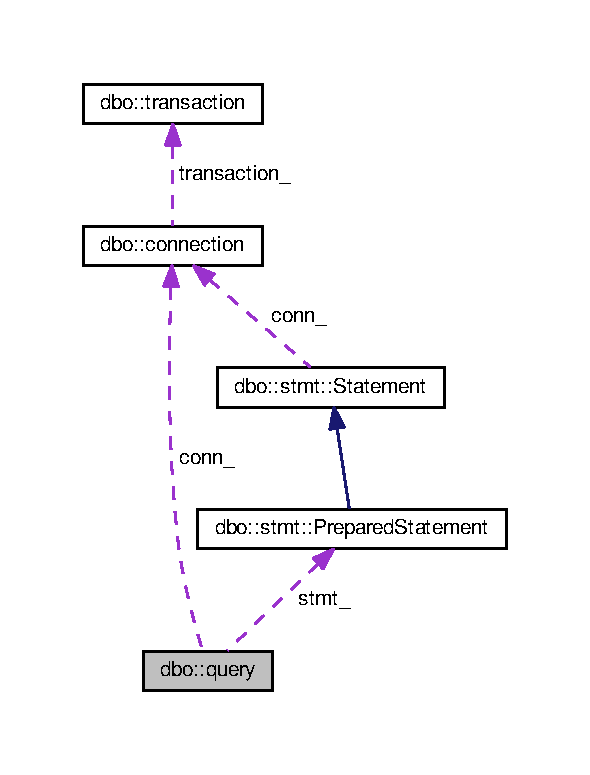
\includegraphics[width=283pt]{classdbo_1_1query__coll__graph}
\end{center}
\end{figure}
\subsection*{Public Member Functions}
\begin{DoxyCompactItemize}
\item 
\hyperlink{classdbo_1_1query_ac19a74e69ad4218112831283f5f0df49}{query} (\hyperlink{classdbo_1_1connection}{connection} \&conn, const std\+::string \&\hyperlink{classdbo_1_1query_a3f8523a194010647409c1d088a873c2b}{sql}=\char`\"{}\char`\"{})
\item 
\hyperlink{classdbo_1_1query_af479777fb57fbf7f857be5369d1c7241}{$\sim$query} ()
\item 
\hyperlink{classdbo_1_1query}{query} \& \hyperlink{classdbo_1_1query_a66350ea5d7bb84e7bdf3499a58afb0c3}{operator=} (const \hyperlink{classdbo_1_1query}{query} \&other)
\item 
{\footnotesize template$<$class C $>$ }\\\hyperlink{classdbo_1_1query}{query} \& \hyperlink{classdbo_1_1query_afc649b97327cf3447938d907251c77d4}{bind} (const C \&value)
\item 
\hyperlink{classdbo_1_1query}{query} \& \hyperlink{classdbo_1_1query_a29e671372b485030cf6dd1ddf6eb9562}{prepare} ()
\item 
\hyperlink{classdbo_1_1query}{query} \& \hyperlink{classdbo_1_1query_add1b7ef5fb795f0cc4c8e026374dde06}{execute} ()
\item 
{\footnotesize template$<$class C $>$ }\\\hyperlink{classdbo_1_1query}{query} \& \hyperlink{classdbo_1_1query_a2a5455a6e17b8807a1c8b8dfddcf9902}{read} (\hyperlink{classdbo_1_1ptr}{ptr}$<$ C $>$ \&\hyperlink{classdbo_1_1ptr}{ptr})
\item 
{\footnotesize template$<$class T $>$ }\\\hyperlink{classdbo_1_1query}{query} \& \hyperlink{classdbo_1_1query_a4b1687876a062d4c8f914bec512e1b36}{read} (T \&value)
\item 
bool \hyperlink{classdbo_1_1query_ae637eeb9728436f0e67d365ac5f85ae1}{next\+Row} ()
\item 
const std\+::string \& \hyperlink{classdbo_1_1query_a3f8523a194010647409c1d088a873c2b}{sql} ()
\item 
bool \hyperlink{classdbo_1_1query_a4b48b4d659f8377cea9976bc9506e354}{hasrow} () const 
\end{DoxyCompactItemize}
\subsection*{Protected Attributes}
\begin{DoxyCompactItemize}
\item 
\hyperlink{classdbo_1_1connection}{connection} $\ast$ \hyperlink{classdbo_1_1query_a284b1502770d8ee9bcae3e5c76939d11}{conn\+\_\+}
\item 
\hyperlink{classdbo_1_1stmt_1_1_prepared_statement}{stmt\+::\+Prepared\+Statement} \hyperlink{classdbo_1_1query_a7402009c90a36d6e941cff2408c89b4e}{stmt\+\_\+}
\item 
std\+::string \hyperlink{classdbo_1_1query_a387fe6e99acb27b15db7ed46979a0b51}{sql\+\_\+}
\item 
bool \hyperlink{classdbo_1_1query_a87d47323c718b28fa479d6cb8ae33703}{prepared\+\_\+}
\item 
bool \hyperlink{classdbo_1_1query_ab345783ac96adcb4373c44bbecb075ef}{hasrow\+\_\+}
\end{DoxyCompactItemize}


\subsection{Constructor \& Destructor Documentation}
\hypertarget{classdbo_1_1query_ac19a74e69ad4218112831283f5f0df49}{\index{dbo\+::query@{dbo\+::query}!query@{query}}
\index{query@{query}!dbo\+::query@{dbo\+::query}}
\subsubsection[{query}]{\setlength{\rightskip}{0pt plus 5cm}query\+::query (
\begin{DoxyParamCaption}
\item[{{\bf connection} \&}]{conn, }
\item[{const std\+::string \&}]{sql = {\ttfamily \char`\"{}\char`\"{}}}
\end{DoxyParamCaption}
)}}\label{classdbo_1_1query_ac19a74e69ad4218112831283f5f0df49}
\hypertarget{classdbo_1_1query_af479777fb57fbf7f857be5369d1c7241}{\index{dbo\+::query@{dbo\+::query}!````~query@{$\sim$query}}
\index{````~query@{$\sim$query}!dbo\+::query@{dbo\+::query}}
\subsubsection[{$\sim$query}]{\setlength{\rightskip}{0pt plus 5cm}query\+::$\sim$query (
\begin{DoxyParamCaption}
{}
\end{DoxyParamCaption}
)}}\label{classdbo_1_1query_af479777fb57fbf7f857be5369d1c7241}


\subsection{Member Function Documentation}
\hypertarget{classdbo_1_1query_afc649b97327cf3447938d907251c77d4}{\index{dbo\+::query@{dbo\+::query}!bind@{bind}}
\index{bind@{bind}!dbo\+::query@{dbo\+::query}}
\subsubsection[{bind}]{\setlength{\rightskip}{0pt plus 5cm}template$<$class C $>$ {\bf query} \& dbo\+::query\+::bind (
\begin{DoxyParamCaption}
\item[{const C \&}]{value}
\end{DoxyParamCaption}
)}}\label{classdbo_1_1query_afc649b97327cf3447938d907251c77d4}
\hypertarget{classdbo_1_1query_add1b7ef5fb795f0cc4c8e026374dde06}{\index{dbo\+::query@{dbo\+::query}!execute@{execute}}
\index{execute@{execute}!dbo\+::query@{dbo\+::query}}
\subsubsection[{execute}]{\setlength{\rightskip}{0pt plus 5cm}{\bf query} \& query\+::execute (
\begin{DoxyParamCaption}
{}
\end{DoxyParamCaption}
)}}\label{classdbo_1_1query_add1b7ef5fb795f0cc4c8e026374dde06}
\hypertarget{classdbo_1_1query_a4b48b4d659f8377cea9976bc9506e354}{\index{dbo\+::query@{dbo\+::query}!hasrow@{hasrow}}
\index{hasrow@{hasrow}!dbo\+::query@{dbo\+::query}}
\subsubsection[{hasrow}]{\setlength{\rightskip}{0pt plus 5cm}bool dbo\+::query\+::hasrow (
\begin{DoxyParamCaption}
{}
\end{DoxyParamCaption}
) const\hspace{0.3cm}{\ttfamily [inline]}}}\label{classdbo_1_1query_a4b48b4d659f8377cea9976bc9506e354}
\hypertarget{classdbo_1_1query_ae637eeb9728436f0e67d365ac5f85ae1}{\index{dbo\+::query@{dbo\+::query}!next\+Row@{next\+Row}}
\index{next\+Row@{next\+Row}!dbo\+::query@{dbo\+::query}}
\subsubsection[{next\+Row}]{\setlength{\rightskip}{0pt plus 5cm}bool query\+::next\+Row (
\begin{DoxyParamCaption}
{}
\end{DoxyParamCaption}
)}}\label{classdbo_1_1query_ae637eeb9728436f0e67d365ac5f85ae1}
\hypertarget{classdbo_1_1query_a66350ea5d7bb84e7bdf3499a58afb0c3}{\index{dbo\+::query@{dbo\+::query}!operator=@{operator=}}
\index{operator=@{operator=}!dbo\+::query@{dbo\+::query}}
\subsubsection[{operator=}]{\setlength{\rightskip}{0pt plus 5cm}{\bf query} \& query\+::operator= (
\begin{DoxyParamCaption}
\item[{const {\bf query} \&}]{other}
\end{DoxyParamCaption}
)}}\label{classdbo_1_1query_a66350ea5d7bb84e7bdf3499a58afb0c3}
\hypertarget{classdbo_1_1query_a29e671372b485030cf6dd1ddf6eb9562}{\index{dbo\+::query@{dbo\+::query}!prepare@{prepare}}
\index{prepare@{prepare}!dbo\+::query@{dbo\+::query}}
\subsubsection[{prepare}]{\setlength{\rightskip}{0pt plus 5cm}{\bf query} \& query\+::prepare (
\begin{DoxyParamCaption}
{}
\end{DoxyParamCaption}
)}}\label{classdbo_1_1query_a29e671372b485030cf6dd1ddf6eb9562}
Prepare the query. Once a query is prepared it becomes a named prepared statement and can not be modified Statements not prepared are executed as anonymous named statements. \hypertarget{classdbo_1_1query_a2a5455a6e17b8807a1c8b8dfddcf9902}{\index{dbo\+::query@{dbo\+::query}!read@{read}}
\index{read@{read}!dbo\+::query@{dbo\+::query}}
\subsubsection[{read}]{\setlength{\rightskip}{0pt plus 5cm}template$<$class C $>$ {\bf query} \& dbo\+::query\+::read (
\begin{DoxyParamCaption}
\item[{{\bf ptr}$<$ C $>$ \&}]{ptr}
\end{DoxyParamCaption}
)}}\label{classdbo_1_1query_a2a5455a6e17b8807a1c8b8dfddcf9902}
\hypertarget{classdbo_1_1query_a4b1687876a062d4c8f914bec512e1b36}{\index{dbo\+::query@{dbo\+::query}!read@{read}}
\index{read@{read}!dbo\+::query@{dbo\+::query}}
\subsubsection[{read}]{\setlength{\rightskip}{0pt plus 5cm}template$<$class T $>$ {\bf query} \& dbo\+::query\+::read (
\begin{DoxyParamCaption}
\item[{T \&}]{value}
\end{DoxyParamCaption}
)}}\label{classdbo_1_1query_a4b1687876a062d4c8f914bec512e1b36}
\hypertarget{classdbo_1_1query_a3f8523a194010647409c1d088a873c2b}{\index{dbo\+::query@{dbo\+::query}!sql@{sql}}
\index{sql@{sql}!dbo\+::query@{dbo\+::query}}
\subsubsection[{sql}]{\setlength{\rightskip}{0pt plus 5cm}const std\+::string\& dbo\+::query\+::sql (
\begin{DoxyParamCaption}
{}
\end{DoxyParamCaption}
)\hspace{0.3cm}{\ttfamily [inline]}}}\label{classdbo_1_1query_a3f8523a194010647409c1d088a873c2b}


\subsection{Member Data Documentation}
\hypertarget{classdbo_1_1query_a284b1502770d8ee9bcae3e5c76939d11}{\index{dbo\+::query@{dbo\+::query}!conn\+\_\+@{conn\+\_\+}}
\index{conn\+\_\+@{conn\+\_\+}!dbo\+::query@{dbo\+::query}}
\subsubsection[{conn\+\_\+}]{\setlength{\rightskip}{0pt plus 5cm}{\bf connection}$\ast$ dbo\+::query\+::conn\+\_\+\hspace{0.3cm}{\ttfamily [protected]}}}\label{classdbo_1_1query_a284b1502770d8ee9bcae3e5c76939d11}
\hypertarget{classdbo_1_1query_ab345783ac96adcb4373c44bbecb075ef}{\index{dbo\+::query@{dbo\+::query}!hasrow\+\_\+@{hasrow\+\_\+}}
\index{hasrow\+\_\+@{hasrow\+\_\+}!dbo\+::query@{dbo\+::query}}
\subsubsection[{hasrow\+\_\+}]{\setlength{\rightskip}{0pt plus 5cm}bool dbo\+::query\+::hasrow\+\_\+\hspace{0.3cm}{\ttfamily [protected]}}}\label{classdbo_1_1query_ab345783ac96adcb4373c44bbecb075ef}
\hypertarget{classdbo_1_1query_a87d47323c718b28fa479d6cb8ae33703}{\index{dbo\+::query@{dbo\+::query}!prepared\+\_\+@{prepared\+\_\+}}
\index{prepared\+\_\+@{prepared\+\_\+}!dbo\+::query@{dbo\+::query}}
\subsubsection[{prepared\+\_\+}]{\setlength{\rightskip}{0pt plus 5cm}bool dbo\+::query\+::prepared\+\_\+\hspace{0.3cm}{\ttfamily [protected]}}}\label{classdbo_1_1query_a87d47323c718b28fa479d6cb8ae33703}
\hypertarget{classdbo_1_1query_a387fe6e99acb27b15db7ed46979a0b51}{\index{dbo\+::query@{dbo\+::query}!sql\+\_\+@{sql\+\_\+}}
\index{sql\+\_\+@{sql\+\_\+}!dbo\+::query@{dbo\+::query}}
\subsubsection[{sql\+\_\+}]{\setlength{\rightskip}{0pt plus 5cm}std\+::string dbo\+::query\+::sql\+\_\+\hspace{0.3cm}{\ttfamily [protected]}}}\label{classdbo_1_1query_a387fe6e99acb27b15db7ed46979a0b51}
\hypertarget{classdbo_1_1query_a7402009c90a36d6e941cff2408c89b4e}{\index{dbo\+::query@{dbo\+::query}!stmt\+\_\+@{stmt\+\_\+}}
\index{stmt\+\_\+@{stmt\+\_\+}!dbo\+::query@{dbo\+::query}}
\subsubsection[{stmt\+\_\+}]{\setlength{\rightskip}{0pt plus 5cm}{\bf stmt\+::\+Prepared\+Statement} dbo\+::query\+::stmt\+\_\+\hspace{0.3cm}{\ttfamily [protected]}}}\label{classdbo_1_1query_a7402009c90a36d6e941cff2408c89b4e}


The documentation for this class was generated from the following files\+:\begin{DoxyCompactItemize}
\item 
dbo/\hyperlink{query_8hpp}{query.\+hpp}\item 
dbo/\hyperlink{query_8cpp}{query.\+cpp}\item 
dbo/\hyperlink{query_8cxx}{query.\+cxx}\end{DoxyCompactItemize}

\hypertarget{classdbo_1_1action_1_1_select_by_id}{\section{dbo\+:\+:action\+:\+:Select\+By\+Id$<$ C $>$ Class Template Reference}
\label{classdbo_1_1action_1_1_select_by_id}\index{dbo\+::action\+::\+Select\+By\+Id$<$ C $>$@{dbo\+::action\+::\+Select\+By\+Id$<$ C $>$}}
}


{\ttfamily \#include $<$Select\+By\+Id.\+hpp$>$}

\subsection*{Public Types}
\begin{DoxyCompactItemize}
\item 
using \hyperlink{classdbo_1_1action_1_1_select_by_id_a00c65e230f8b64b90713042403032403}{Id\+Type} = typename \hyperlink{structdbo_1_1traits_1_1dbo__traits}{traits\+::dbo\+\_\+traits}$<$ C $>$\+::\hyperlink{classdbo_1_1action_1_1_select_by_id_a00c65e230f8b64b90713042403032403}{Id\+Type}
\end{DoxyCompactItemize}
\subsection*{Public Member Functions}
\begin{DoxyCompactItemize}
\item 
\hyperlink{classdbo_1_1action_1_1_select_by_id_a6b7285e0f00b4cd5f0e9cc7502baf9b9}{Select\+By\+Id} (\hyperlink{classdbo_1_1ptr}{ptr}$<$ C $>$ \hyperlink{classdbo_1_1ptr}{ptr}, std\+::shared\+\_\+ptr$<$ \hyperlink{classdbo_1_1mapping_1_1_mapping}{mapping\+::\+Mapping}$<$ C $>$$>$ mapping, \hyperlink{classdbo_1_1stmt_1_1_prepared_statement}{stmt\+::\+Prepared\+Statement} \&stmt)
\item 
\hyperlink{classdbo_1_1action_1_1_select_by_id_a4e8428400825076ddd90c995cc6cdfcb}{Select\+By\+Id} (\hyperlink{classdbo_1_1ptr}{ptr}$<$ C $>$ \hyperlink{classdbo_1_1ptr}{ptr}, \hyperlink{classdbo_1_1action_1_1_select_by_id_a00c65e230f8b64b90713042403032403}{Id\+Type} \hyperlink{namespacedbo_a8d25907296ae8360b3120b7492022c1d}{id}, std\+::shared\+\_\+ptr$<$ \hyperlink{classdbo_1_1mapping_1_1_mapping}{mapping\+::\+Mapping}$<$ C $>$$>$ mapping, \hyperlink{classdbo_1_1stmt_1_1_prepared_statement}{stmt\+::\+Prepared\+Statement} \&stmt)
\item 
void \hyperlink{classdbo_1_1action_1_1_select_by_id_a5567027d84c59654bcf83f7dd5c175ee}{visit} ()
\item 
{\footnotesize template$<$typename V $>$ }\\void \hyperlink{classdbo_1_1action_1_1_select_by_id_a835e329a94a4f3a1b3c6dff876a3a06d}{act} (const \hyperlink{classdbo_1_1mapping_1_1_field_ref}{mapping\+::\+Field\+Ref}$<$ V $>$ \&\hyperlink{namespacedbo_ad1f50f02cb050acf946807959252a93f}{field})
\item 
{\footnotesize template$<$typename V $>$ }\\void \hyperlink{classdbo_1_1action_1_1_select_by_id_ade0aeba44536864743ad2f12536b7094}{act\+Id} (V \&value, const std\+::string \&name, int size)
\item 
{\footnotesize template$<$class D $>$ }\\void \hyperlink{classdbo_1_1action_1_1_select_by_id_a6e71df03fb61fe01363a6db4f86eb637}{act\+Id} (\hyperlink{classdbo_1_1ptr}{ptr}$<$ D $>$ \&value, const std\+::string \&name, int size, int fk\+Constraints)
\item 
{\footnotesize template$<$class D $>$ }\\void \hyperlink{classdbo_1_1action_1_1_select_by_id_a832cf6f330506ea92a64454a3fe45626}{act\+Ptr} (const \hyperlink{classdbo_1_1mapping_1_1_ptr_ref}{mapping\+::\+Ptr\+Ref}$<$ D $>$ \&\hyperlink{namespacedbo_ad1f50f02cb050acf946807959252a93f}{field})
\item 
\hyperlink{classdbo_1_1connection}{connection} \& \hyperlink{classdbo_1_1action_1_1_select_by_id_ad5a0b639d9d4084e6ba34cf919c530ae}{conn} ()
\end{DoxyCompactItemize}
\subsection*{Friends}
\begin{DoxyCompactItemize}
\item 
{\footnotesize template$<$class D $>$ }\\class \hyperlink{classdbo_1_1action_1_1_select_by_id_a9952e8f41a3fb1af7b01c5ed0892a551}{Select\+By\+Id}
\end{DoxyCompactItemize}


\subsection{Member Typedef Documentation}
\hypertarget{classdbo_1_1action_1_1_select_by_id_a00c65e230f8b64b90713042403032403}{\index{dbo\+::action\+::\+Select\+By\+Id@{dbo\+::action\+::\+Select\+By\+Id}!Id\+Type@{Id\+Type}}
\index{Id\+Type@{Id\+Type}!dbo\+::action\+::\+Select\+By\+Id@{dbo\+::action\+::\+Select\+By\+Id}}
\subsubsection[{Id\+Type}]{\setlength{\rightskip}{0pt plus 5cm}template$<$class C $>$ using {\bf dbo\+::action\+::\+Select\+By\+Id}$<$ C $>$\+::{\bf Id\+Type} =  typename {\bf traits\+::dbo\+\_\+traits}$<$C$>$\+::{\bf Id\+Type}}}\label{classdbo_1_1action_1_1_select_by_id_a00c65e230f8b64b90713042403032403}


\subsection{Constructor \& Destructor Documentation}
\hypertarget{classdbo_1_1action_1_1_select_by_id_a6b7285e0f00b4cd5f0e9cc7502baf9b9}{\index{dbo\+::action\+::\+Select\+By\+Id@{dbo\+::action\+::\+Select\+By\+Id}!Select\+By\+Id@{Select\+By\+Id}}
\index{Select\+By\+Id@{Select\+By\+Id}!dbo\+::action\+::\+Select\+By\+Id@{dbo\+::action\+::\+Select\+By\+Id}}
\subsubsection[{Select\+By\+Id}]{\setlength{\rightskip}{0pt plus 5cm}template$<$class C $>$ {\bf dbo\+::action\+::\+Select\+By\+Id}$<$ C $>$\+::{\bf Select\+By\+Id} (
\begin{DoxyParamCaption}
\item[{{\bf ptr}$<$ C $>$}]{ptr, }
\item[{std\+::shared\+\_\+ptr$<$ {\bf mapping\+::\+Mapping}$<$ C $>$$>$}]{mapping, }
\item[{{\bf stmt\+::\+Prepared\+Statement} \&}]{stmt}
\end{DoxyParamCaption}
)}}\label{classdbo_1_1action_1_1_select_by_id_a6b7285e0f00b4cd5f0e9cc7502baf9b9}
\hypertarget{classdbo_1_1action_1_1_select_by_id_a4e8428400825076ddd90c995cc6cdfcb}{\index{dbo\+::action\+::\+Select\+By\+Id@{dbo\+::action\+::\+Select\+By\+Id}!Select\+By\+Id@{Select\+By\+Id}}
\index{Select\+By\+Id@{Select\+By\+Id}!dbo\+::action\+::\+Select\+By\+Id@{dbo\+::action\+::\+Select\+By\+Id}}
\subsubsection[{Select\+By\+Id}]{\setlength{\rightskip}{0pt plus 5cm}template$<$class C $>$ {\bf dbo\+::action\+::\+Select\+By\+Id}$<$ C $>$\+::{\bf Select\+By\+Id} (
\begin{DoxyParamCaption}
\item[{{\bf ptr}$<$ C $>$}]{ptr, }
\item[{{\bf Id\+Type}}]{id, }
\item[{std\+::shared\+\_\+ptr$<$ {\bf mapping\+::\+Mapping}$<$ C $>$$>$}]{mapping, }
\item[{{\bf stmt\+::\+Prepared\+Statement} \&}]{stmt}
\end{DoxyParamCaption}
)}}\label{classdbo_1_1action_1_1_select_by_id_a4e8428400825076ddd90c995cc6cdfcb}


\subsection{Member Function Documentation}
\hypertarget{classdbo_1_1action_1_1_select_by_id_a835e329a94a4f3a1b3c6dff876a3a06d}{\index{dbo\+::action\+::\+Select\+By\+Id@{dbo\+::action\+::\+Select\+By\+Id}!act@{act}}
\index{act@{act}!dbo\+::action\+::\+Select\+By\+Id@{dbo\+::action\+::\+Select\+By\+Id}}
\subsubsection[{act}]{\setlength{\rightskip}{0pt plus 5cm}template$<$class C $>$ template$<$typename V $>$ void {\bf dbo\+::action\+::\+Select\+By\+Id}$<$ C $>$\+::act (
\begin{DoxyParamCaption}
\item[{const {\bf mapping\+::\+Field\+Ref}$<$ V $>$ \&}]{field}
\end{DoxyParamCaption}
)}}\label{classdbo_1_1action_1_1_select_by_id_a835e329a94a4f3a1b3c6dff876a3a06d}
\hypertarget{classdbo_1_1action_1_1_select_by_id_ade0aeba44536864743ad2f12536b7094}{\index{dbo\+::action\+::\+Select\+By\+Id@{dbo\+::action\+::\+Select\+By\+Id}!act\+Id@{act\+Id}}
\index{act\+Id@{act\+Id}!dbo\+::action\+::\+Select\+By\+Id@{dbo\+::action\+::\+Select\+By\+Id}}
\subsubsection[{act\+Id}]{\setlength{\rightskip}{0pt plus 5cm}template$<$class C $>$ template$<$typename V $>$ void {\bf dbo\+::action\+::\+Select\+By\+Id}$<$ C $>$\+::act\+Id (
\begin{DoxyParamCaption}
\item[{V \&}]{value, }
\item[{const std\+::string \&}]{name, }
\item[{int}]{size}
\end{DoxyParamCaption}
)}}\label{classdbo_1_1action_1_1_select_by_id_ade0aeba44536864743ad2f12536b7094}
\hypertarget{classdbo_1_1action_1_1_select_by_id_a6e71df03fb61fe01363a6db4f86eb637}{\index{dbo\+::action\+::\+Select\+By\+Id@{dbo\+::action\+::\+Select\+By\+Id}!act\+Id@{act\+Id}}
\index{act\+Id@{act\+Id}!dbo\+::action\+::\+Select\+By\+Id@{dbo\+::action\+::\+Select\+By\+Id}}
\subsubsection[{act\+Id}]{\setlength{\rightskip}{0pt plus 5cm}template$<$class C $>$ template$<$class D $>$ void {\bf dbo\+::action\+::\+Select\+By\+Id}$<$ C $>$\+::act\+Id (
\begin{DoxyParamCaption}
\item[{{\bf ptr}$<$ D $>$ \&}]{value, }
\item[{const std\+::string \&}]{name, }
\item[{int}]{size, }
\item[{int}]{fk\+Constraints}
\end{DoxyParamCaption}
)}}\label{classdbo_1_1action_1_1_select_by_id_a6e71df03fb61fe01363a6db4f86eb637}
\hypertarget{classdbo_1_1action_1_1_select_by_id_a832cf6f330506ea92a64454a3fe45626}{\index{dbo\+::action\+::\+Select\+By\+Id@{dbo\+::action\+::\+Select\+By\+Id}!act\+Ptr@{act\+Ptr}}
\index{act\+Ptr@{act\+Ptr}!dbo\+::action\+::\+Select\+By\+Id@{dbo\+::action\+::\+Select\+By\+Id}}
\subsubsection[{act\+Ptr}]{\setlength{\rightskip}{0pt plus 5cm}template$<$class C $>$ template$<$class D $>$ void {\bf dbo\+::action\+::\+Select\+By\+Id}$<$ C $>$\+::act\+Ptr (
\begin{DoxyParamCaption}
\item[{const {\bf mapping\+::\+Ptr\+Ref}$<$ D $>$ \&}]{field}
\end{DoxyParamCaption}
)}}\label{classdbo_1_1action_1_1_select_by_id_a832cf6f330506ea92a64454a3fe45626}
\hypertarget{classdbo_1_1action_1_1_select_by_id_ad5a0b639d9d4084e6ba34cf919c530ae}{\index{dbo\+::action\+::\+Select\+By\+Id@{dbo\+::action\+::\+Select\+By\+Id}!conn@{conn}}
\index{conn@{conn}!dbo\+::action\+::\+Select\+By\+Id@{dbo\+::action\+::\+Select\+By\+Id}}
\subsubsection[{conn}]{\setlength{\rightskip}{0pt plus 5cm}template$<$class C $>$ {\bf connection}\& {\bf dbo\+::action\+::\+Select\+By\+Id}$<$ C $>$\+::conn (
\begin{DoxyParamCaption}
{}
\end{DoxyParamCaption}
)\hspace{0.3cm}{\ttfamily [inline]}}}\label{classdbo_1_1action_1_1_select_by_id_ad5a0b639d9d4084e6ba34cf919c530ae}
\hypertarget{classdbo_1_1action_1_1_select_by_id_a5567027d84c59654bcf83f7dd5c175ee}{\index{dbo\+::action\+::\+Select\+By\+Id@{dbo\+::action\+::\+Select\+By\+Id}!visit@{visit}}
\index{visit@{visit}!dbo\+::action\+::\+Select\+By\+Id@{dbo\+::action\+::\+Select\+By\+Id}}
\subsubsection[{visit}]{\setlength{\rightskip}{0pt plus 5cm}template$<$class C $>$ void {\bf dbo\+::action\+::\+Select\+By\+Id}$<$ C $>$\+::visit (
\begin{DoxyParamCaption}
{}
\end{DoxyParamCaption}
)}}\label{classdbo_1_1action_1_1_select_by_id_a5567027d84c59654bcf83f7dd5c175ee}


\subsection{Friends And Related Function Documentation}
\hypertarget{classdbo_1_1action_1_1_select_by_id_a9952e8f41a3fb1af7b01c5ed0892a551}{\index{dbo\+::action\+::\+Select\+By\+Id@{dbo\+::action\+::\+Select\+By\+Id}!Select\+By\+Id@{Select\+By\+Id}}
\index{Select\+By\+Id@{Select\+By\+Id}!dbo\+::action\+::\+Select\+By\+Id@{dbo\+::action\+::\+Select\+By\+Id}}
\subsubsection[{Select\+By\+Id}]{\setlength{\rightskip}{0pt plus 5cm}template$<$class C $>$ template$<$class D $>$ friend class {\bf Select\+By\+Id}\hspace{0.3cm}{\ttfamily [friend]}}}\label{classdbo_1_1action_1_1_select_by_id_a9952e8f41a3fb1af7b01c5ed0892a551}


The documentation for this class was generated from the following files\+:\begin{DoxyCompactItemize}
\item 
dbo/action/\hyperlink{_select_by_id_8hpp}{Select\+By\+Id.\+hpp}\item 
dbo/action/\hyperlink{_select_by_id_8cxx}{Select\+By\+Id.\+cxx}\end{DoxyCompactItemize}

\hypertarget{structdbo_1_1mapping_1_1_set_info}{\section{dbo\+:\+:mapping\+:\+:Set\+Info Struct Reference}
\label{structdbo_1_1mapping_1_1_set_info}\index{dbo\+::mapping\+::\+Set\+Info@{dbo\+::mapping\+::\+Set\+Info}}
}


{\ttfamily \#include $<$Set\+Info.\+h$>$}

\subsection*{Public Member Functions}
\begin{DoxyCompactItemize}
\item 
\hyperlink{structdbo_1_1mapping_1_1_set_info_a089ee965269d4a8538f82e11540ad26f}{Set\+Info} (std\+::string table\+Name, \hyperlink{namespacedbo_ab7f92e64aea13b1e3b60021e72a9fc73}{Relation\+Type} type, const std\+::string \&join\+Name, const std\+::string \&join\+Self\+Id, int some\+Fk\+Constraints)
\item 
std\+::string \hyperlink{structdbo_1_1mapping_1_1_set_info_adb66cca5ff652c1bc5cea8f25d0142b2}{debug} (int tab)
\end{DoxyCompactItemize}
\subsection*{Public Attributes}
\begin{DoxyCompactItemize}
\item 
std\+::string \hyperlink{structdbo_1_1mapping_1_1_set_info_a15381af2c3f8d8341b006633df78eade}{table\+Name\+\_\+}
\item 
std\+::string \hyperlink{structdbo_1_1mapping_1_1_set_info_ae400d74bc9aee243a56ade82510a0d8e}{join\+Name\+\_\+}
\item 
std\+::string \hyperlink{structdbo_1_1mapping_1_1_set_info_acce28d7bd0a498487f56801eab1dfb86}{join\+Self\+Id\+\_\+}
\item 
std\+::string \hyperlink{structdbo_1_1mapping_1_1_set_info_a590227560e9e15aeca0f0f6215c64f25}{join\+Other\+Id\+\_\+}
\item 
\hyperlink{namespacedbo_ab7f92e64aea13b1e3b60021e72a9fc73}{Relation\+Type} \hyperlink{structdbo_1_1mapping_1_1_set_info_a8e23d703a1fe265a10f4cdb335cb488e}{type\+\_\+}
\item 
int \hyperlink{structdbo_1_1mapping_1_1_set_info_a8ee87d40f0f835482282c804c309c968}{fk\+Constraints\+\_\+}
\item 
int \hyperlink{structdbo_1_1mapping_1_1_set_info_a05c008084f20eb52f7f1145be419d2f1}{other\+Fk\+Constraints\+\_\+}
\end{DoxyCompactItemize}


\subsection{Constructor \& Destructor Documentation}
\hypertarget{structdbo_1_1mapping_1_1_set_info_a089ee965269d4a8538f82e11540ad26f}{\index{dbo\+::mapping\+::\+Set\+Info@{dbo\+::mapping\+::\+Set\+Info}!Set\+Info@{Set\+Info}}
\index{Set\+Info@{Set\+Info}!dbo\+::mapping\+::\+Set\+Info@{dbo\+::mapping\+::\+Set\+Info}}
\subsubsection[{Set\+Info}]{\setlength{\rightskip}{0pt plus 5cm}dbo\+::mapping\+::\+Set\+Info\+::\+Set\+Info (
\begin{DoxyParamCaption}
\item[{std\+::string}]{table\+Name, }
\item[{{\bf Relation\+Type}}]{type, }
\item[{const std\+::string \&}]{join\+Name, }
\item[{const std\+::string \&}]{join\+Self\+Id, }
\item[{int}]{some\+Fk\+Constraints}
\end{DoxyParamCaption}
)\hspace{0.3cm}{\ttfamily [inline]}}}\label{structdbo_1_1mapping_1_1_set_info_a089ee965269d4a8538f82e11540ad26f}


\subsection{Member Function Documentation}
\hypertarget{structdbo_1_1mapping_1_1_set_info_adb66cca5ff652c1bc5cea8f25d0142b2}{\index{dbo\+::mapping\+::\+Set\+Info@{dbo\+::mapping\+::\+Set\+Info}!debug@{debug}}
\index{debug@{debug}!dbo\+::mapping\+::\+Set\+Info@{dbo\+::mapping\+::\+Set\+Info}}
\subsubsection[{debug}]{\setlength{\rightskip}{0pt plus 5cm}std\+::string dbo\+::mapping\+::\+Set\+Info\+::debug (
\begin{DoxyParamCaption}
\item[{int}]{tab}
\end{DoxyParamCaption}
)\hspace{0.3cm}{\ttfamily [inline]}}}\label{structdbo_1_1mapping_1_1_set_info_adb66cca5ff652c1bc5cea8f25d0142b2}


\subsection{Member Data Documentation}
\hypertarget{structdbo_1_1mapping_1_1_set_info_a8ee87d40f0f835482282c804c309c968}{\index{dbo\+::mapping\+::\+Set\+Info@{dbo\+::mapping\+::\+Set\+Info}!fk\+Constraints\+\_\+@{fk\+Constraints\+\_\+}}
\index{fk\+Constraints\+\_\+@{fk\+Constraints\+\_\+}!dbo\+::mapping\+::\+Set\+Info@{dbo\+::mapping\+::\+Set\+Info}}
\subsubsection[{fk\+Constraints\+\_\+}]{\setlength{\rightskip}{0pt plus 5cm}int dbo\+::mapping\+::\+Set\+Info\+::fk\+Constraints\+\_\+}}\label{structdbo_1_1mapping_1_1_set_info_a8ee87d40f0f835482282c804c309c968}
\hypertarget{structdbo_1_1mapping_1_1_set_info_ae400d74bc9aee243a56ade82510a0d8e}{\index{dbo\+::mapping\+::\+Set\+Info@{dbo\+::mapping\+::\+Set\+Info}!join\+Name\+\_\+@{join\+Name\+\_\+}}
\index{join\+Name\+\_\+@{join\+Name\+\_\+}!dbo\+::mapping\+::\+Set\+Info@{dbo\+::mapping\+::\+Set\+Info}}
\subsubsection[{join\+Name\+\_\+}]{\setlength{\rightskip}{0pt plus 5cm}std\+::string dbo\+::mapping\+::\+Set\+Info\+::join\+Name\+\_\+}}\label{structdbo_1_1mapping_1_1_set_info_ae400d74bc9aee243a56ade82510a0d8e}
\hypertarget{structdbo_1_1mapping_1_1_set_info_a590227560e9e15aeca0f0f6215c64f25}{\index{dbo\+::mapping\+::\+Set\+Info@{dbo\+::mapping\+::\+Set\+Info}!join\+Other\+Id\+\_\+@{join\+Other\+Id\+\_\+}}
\index{join\+Other\+Id\+\_\+@{join\+Other\+Id\+\_\+}!dbo\+::mapping\+::\+Set\+Info@{dbo\+::mapping\+::\+Set\+Info}}
\subsubsection[{join\+Other\+Id\+\_\+}]{\setlength{\rightskip}{0pt plus 5cm}std\+::string dbo\+::mapping\+::\+Set\+Info\+::join\+Other\+Id\+\_\+}}\label{structdbo_1_1mapping_1_1_set_info_a590227560e9e15aeca0f0f6215c64f25}
\hypertarget{structdbo_1_1mapping_1_1_set_info_acce28d7bd0a498487f56801eab1dfb86}{\index{dbo\+::mapping\+::\+Set\+Info@{dbo\+::mapping\+::\+Set\+Info}!join\+Self\+Id\+\_\+@{join\+Self\+Id\+\_\+}}
\index{join\+Self\+Id\+\_\+@{join\+Self\+Id\+\_\+}!dbo\+::mapping\+::\+Set\+Info@{dbo\+::mapping\+::\+Set\+Info}}
\subsubsection[{join\+Self\+Id\+\_\+}]{\setlength{\rightskip}{0pt plus 5cm}std\+::string dbo\+::mapping\+::\+Set\+Info\+::join\+Self\+Id\+\_\+}}\label{structdbo_1_1mapping_1_1_set_info_acce28d7bd0a498487f56801eab1dfb86}
\hypertarget{structdbo_1_1mapping_1_1_set_info_a05c008084f20eb52f7f1145be419d2f1}{\index{dbo\+::mapping\+::\+Set\+Info@{dbo\+::mapping\+::\+Set\+Info}!other\+Fk\+Constraints\+\_\+@{other\+Fk\+Constraints\+\_\+}}
\index{other\+Fk\+Constraints\+\_\+@{other\+Fk\+Constraints\+\_\+}!dbo\+::mapping\+::\+Set\+Info@{dbo\+::mapping\+::\+Set\+Info}}
\subsubsection[{other\+Fk\+Constraints\+\_\+}]{\setlength{\rightskip}{0pt plus 5cm}int dbo\+::mapping\+::\+Set\+Info\+::other\+Fk\+Constraints\+\_\+}}\label{structdbo_1_1mapping_1_1_set_info_a05c008084f20eb52f7f1145be419d2f1}
\hypertarget{structdbo_1_1mapping_1_1_set_info_a15381af2c3f8d8341b006633df78eade}{\index{dbo\+::mapping\+::\+Set\+Info@{dbo\+::mapping\+::\+Set\+Info}!table\+Name\+\_\+@{table\+Name\+\_\+}}
\index{table\+Name\+\_\+@{table\+Name\+\_\+}!dbo\+::mapping\+::\+Set\+Info@{dbo\+::mapping\+::\+Set\+Info}}
\subsubsection[{table\+Name\+\_\+}]{\setlength{\rightskip}{0pt plus 5cm}std\+::string dbo\+::mapping\+::\+Set\+Info\+::table\+Name\+\_\+}}\label{structdbo_1_1mapping_1_1_set_info_a15381af2c3f8d8341b006633df78eade}
\hypertarget{structdbo_1_1mapping_1_1_set_info_a8e23d703a1fe265a10f4cdb335cb488e}{\index{dbo\+::mapping\+::\+Set\+Info@{dbo\+::mapping\+::\+Set\+Info}!type\+\_\+@{type\+\_\+}}
\index{type\+\_\+@{type\+\_\+}!dbo\+::mapping\+::\+Set\+Info@{dbo\+::mapping\+::\+Set\+Info}}
\subsubsection[{type\+\_\+}]{\setlength{\rightskip}{0pt plus 5cm}{\bf Relation\+Type} dbo\+::mapping\+::\+Set\+Info\+::type\+\_\+}}\label{structdbo_1_1mapping_1_1_set_info_a8e23d703a1fe265a10f4cdb335cb488e}


The documentation for this struct was generated from the following file\+:\begin{DoxyCompactItemize}
\item 
dbo/mapping/\hyperlink{_set_info_8h}{Set\+Info.\+h}\end{DoxyCompactItemize}

\hypertarget{structdbo_1_1traits_1_1sql__value__traits}{\section{dbo\+:\+:traits\+:\+:sql\+\_\+value\+\_\+traits$<$ V, Enable $>$ Class Template Reference}
\label{structdbo_1_1traits_1_1sql__value__traits}\index{dbo\+::traits\+::sql\+\_\+value\+\_\+traits$<$ V, Enable $>$@{dbo\+::traits\+::sql\+\_\+value\+\_\+traits$<$ V, Enable $>$}}
}


Traits class for value types.  




{\ttfamily \#include $<$sql\+\_\+value\+\_\+traits.\+hpp$>$}

\subsection*{Static Public Attributes}
\begin{DoxyCompactItemize}
\item 
static const bool \hyperlink{structdbo_1_1traits_1_1sql__value__traits_ac05f51eeec8be981aa7be0aac21858be}{not\+\_\+specialized} =true
\end{DoxyCompactItemize}


\subsection{Detailed Description}
\subsubsection*{template$<$typename V, class Enable = void$>$class dbo\+::traits\+::sql\+\_\+value\+\_\+traits$<$ V, Enable $>$}

Traits class for value types. 

This traits class may be specialized for a custom type {\ttfamily V}, to add dbo support for custom types. A value type has a one-\/to-\/one mapping to a single database column.

The library has built-\/in support for\+:
\begin{DoxyItemize}
\item {\ttfamily std\+::string}
\item {\ttfamily char const $\ast$} (read-\/only\+: only as a bound parameter for a query)
\item {\ttfamily short}, {\ttfamily int}, {\ttfamily long long}
\item {\ttfamily long}\+: since the size of a {\ttfamily long} is 64bit on U\+N\+I\+X/\+Linux 64bit systems and 32bit otherwise, it is mapped to an {\ttfamily integer} or a {\ttfamily bigint} depending on the environment.
\item {\ttfamily float}, {\ttfamily double}
\item enum types
\item {\ttfamily bool}
\item {\ttfamily std\+::vector$<$unsigned char$>$} (binary data)
\item {\ttfamily boost\+::optional$<$\+T$>$}\+: to make the type optional (allowing an S\+Q\+L {\ttfamily null} value)
\item {\ttfamily boost\+::posix\+\_\+time\+::ptime}\+: time stamp, an invalid value (e.\+g. default constructed), maps to {\ttfamily null}
\item {\ttfamily boost\+::posix\+\_\+time\+::time\+\_\+duration}\+: time interval, an invalid value (boost\+::posix\+\_\+time\+::not\+\_\+a\+\_\+date\+\_\+time), maps to {\ttfamily null}
\end{DoxyItemize}

\begin{DoxySeeAlso}{See also}
query\+\_\+result\+\_\+traits 
\end{DoxySeeAlso}


\subsection{Member Data Documentation}
\hypertarget{structdbo_1_1traits_1_1sql__value__traits_ac05f51eeec8be981aa7be0aac21858be}{\index{dbo\+::traits\+::sql\+\_\+value\+\_\+traits@{dbo\+::traits\+::sql\+\_\+value\+\_\+traits}!not\+\_\+specialized@{not\+\_\+specialized}}
\index{not\+\_\+specialized@{not\+\_\+specialized}!dbo\+::traits\+::sql\+\_\+value\+\_\+traits@{dbo\+::traits\+::sql\+\_\+value\+\_\+traits}}
\subsubsection[{not\+\_\+specialized}]{\setlength{\rightskip}{0pt plus 5cm}template$<$typename V, class Enable  = void$>$ const bool {\bf dbo\+::traits\+::sql\+\_\+value\+\_\+traits}$<$ V, Enable $>$\+::not\+\_\+specialized =true\hspace{0.3cm}{\ttfamily [static]}}}\label{structdbo_1_1traits_1_1sql__value__traits_ac05f51eeec8be981aa7be0aac21858be}


The documentation for this class was generated from the following file\+:\begin{DoxyCompactItemize}
\item 
dbo/traits/\hyperlink{sql__value__traits_8hpp}{sql\+\_\+value\+\_\+traits.\+hpp}\end{DoxyCompactItemize}

\hypertarget{structdbo_1_1traits_1_1sql__value__traits_3_01bool_00_01void_01_4}{\section{dbo\+:\+:traits\+:\+:sql\+\_\+value\+\_\+traits$<$ bool, void $>$ Struct Template Reference}
\label{structdbo_1_1traits_1_1sql__value__traits_3_01bool_00_01void_01_4}\index{dbo\+::traits\+::sql\+\_\+value\+\_\+traits$<$ bool, void $>$@{dbo\+::traits\+::sql\+\_\+value\+\_\+traits$<$ bool, void $>$}}
}


{\ttfamily \#include $<$Std\+Sql\+Traits.\+h$>$}

\subsection*{Static Public Member Functions}
\begin{DoxyCompactItemize}
\item 
static std\+::string \hyperlink{structdbo_1_1traits_1_1sql__value__traits_3_01bool_00_01void_01_4_a369a4f0fa91607e2d27d3cc208bec8b5}{type} (int size)
\item 
static void \hyperlink{structdbo_1_1traits_1_1sql__value__traits_3_01bool_00_01void_01_4_a53a10a7a5033298bb69478205335ba29}{bind} (bool v, \hyperlink{classdbo_1_1stmt_1_1_statement}{stmt\+::\+Statement} \&statement, int size)
\item 
static bool \hyperlink{structdbo_1_1traits_1_1sql__value__traits_3_01bool_00_01void_01_4_a5da071bdd96e4eb6193681a9434885ad}{read} (bool \&v, \hyperlink{classdbo_1_1stmt_1_1_statement}{stmt\+::\+Statement} \&statement, int size)
\end{DoxyCompactItemize}
\subsection*{Static Public Attributes}
\begin{DoxyCompactItemize}
\item 
static const bool \hyperlink{structdbo_1_1traits_1_1sql__value__traits_3_01bool_00_01void_01_4_afb605bed7de8a0b5dc939f9a3fa9e1cc}{specialized} =true
\end{DoxyCompactItemize}


\subsection{Member Function Documentation}
\hypertarget{structdbo_1_1traits_1_1sql__value__traits_3_01bool_00_01void_01_4_a53a10a7a5033298bb69478205335ba29}{\index{dbo\+::traits\+::sql\+\_\+value\+\_\+traits$<$ bool, void $>$@{dbo\+::traits\+::sql\+\_\+value\+\_\+traits$<$ bool, void $>$}!bind@{bind}}
\index{bind@{bind}!dbo\+::traits\+::sql\+\_\+value\+\_\+traits$<$ bool, void $>$@{dbo\+::traits\+::sql\+\_\+value\+\_\+traits$<$ bool, void $>$}}
\subsubsection[{bind}]{\setlength{\rightskip}{0pt plus 5cm}static void {\bf dbo\+::traits\+::sql\+\_\+value\+\_\+traits}$<$ bool, void $>$\+::bind (
\begin{DoxyParamCaption}
\item[{bool}]{v, }
\item[{{\bf stmt\+::\+Statement} \&}]{statement, }
\item[{int}]{size}
\end{DoxyParamCaption}
)\hspace{0.3cm}{\ttfamily [static]}}}\label{structdbo_1_1traits_1_1sql__value__traits_3_01bool_00_01void_01_4_a53a10a7a5033298bb69478205335ba29}
\hypertarget{structdbo_1_1traits_1_1sql__value__traits_3_01bool_00_01void_01_4_a5da071bdd96e4eb6193681a9434885ad}{\index{dbo\+::traits\+::sql\+\_\+value\+\_\+traits$<$ bool, void $>$@{dbo\+::traits\+::sql\+\_\+value\+\_\+traits$<$ bool, void $>$}!read@{read}}
\index{read@{read}!dbo\+::traits\+::sql\+\_\+value\+\_\+traits$<$ bool, void $>$@{dbo\+::traits\+::sql\+\_\+value\+\_\+traits$<$ bool, void $>$}}
\subsubsection[{read}]{\setlength{\rightskip}{0pt plus 5cm}static bool {\bf dbo\+::traits\+::sql\+\_\+value\+\_\+traits}$<$ bool, void $>$\+::read (
\begin{DoxyParamCaption}
\item[{bool \&}]{v, }
\item[{{\bf stmt\+::\+Statement} \&}]{statement, }
\item[{int}]{size}
\end{DoxyParamCaption}
)\hspace{0.3cm}{\ttfamily [static]}}}\label{structdbo_1_1traits_1_1sql__value__traits_3_01bool_00_01void_01_4_a5da071bdd96e4eb6193681a9434885ad}
\hypertarget{structdbo_1_1traits_1_1sql__value__traits_3_01bool_00_01void_01_4_a369a4f0fa91607e2d27d3cc208bec8b5}{\index{dbo\+::traits\+::sql\+\_\+value\+\_\+traits$<$ bool, void $>$@{dbo\+::traits\+::sql\+\_\+value\+\_\+traits$<$ bool, void $>$}!type@{type}}
\index{type@{type}!dbo\+::traits\+::sql\+\_\+value\+\_\+traits$<$ bool, void $>$@{dbo\+::traits\+::sql\+\_\+value\+\_\+traits$<$ bool, void $>$}}
\subsubsection[{type}]{\setlength{\rightskip}{0pt plus 5cm}static std\+::string {\bf dbo\+::traits\+::sql\+\_\+value\+\_\+traits}$<$ bool, void $>$\+::type (
\begin{DoxyParamCaption}
\item[{int}]{size}
\end{DoxyParamCaption}
)\hspace{0.3cm}{\ttfamily [static]}}}\label{structdbo_1_1traits_1_1sql__value__traits_3_01bool_00_01void_01_4_a369a4f0fa91607e2d27d3cc208bec8b5}


\subsection{Member Data Documentation}
\hypertarget{structdbo_1_1traits_1_1sql__value__traits_3_01bool_00_01void_01_4_afb605bed7de8a0b5dc939f9a3fa9e1cc}{\index{dbo\+::traits\+::sql\+\_\+value\+\_\+traits$<$ bool, void $>$@{dbo\+::traits\+::sql\+\_\+value\+\_\+traits$<$ bool, void $>$}!specialized@{specialized}}
\index{specialized@{specialized}!dbo\+::traits\+::sql\+\_\+value\+\_\+traits$<$ bool, void $>$@{dbo\+::traits\+::sql\+\_\+value\+\_\+traits$<$ bool, void $>$}}
\subsubsection[{specialized}]{\setlength{\rightskip}{0pt plus 5cm}const bool {\bf dbo\+::traits\+::sql\+\_\+value\+\_\+traits}$<$ bool, void $>$\+::specialized =true\hspace{0.3cm}{\ttfamily [static]}}}\label{structdbo_1_1traits_1_1sql__value__traits_3_01bool_00_01void_01_4_afb605bed7de8a0b5dc939f9a3fa9e1cc}


The documentation for this struct was generated from the following file\+:\begin{DoxyCompactItemize}
\item 
dbo/traits/\hyperlink{_std_sql_traits_8h}{Std\+Sql\+Traits.\+h}\end{DoxyCompactItemize}

\hypertarget{structdbo_1_1traits_1_1sql__value__traits_3_01boost_1_1gregorian_1_1date_00_01void_01_4}{\section{dbo\+:\+:traits\+:\+:sql\+\_\+value\+\_\+traits$<$ boost\+:\+:gregorian\+:\+:date, void $>$ Struct Template Reference}
\label{structdbo_1_1traits_1_1sql__value__traits_3_01boost_1_1gregorian_1_1date_00_01void_01_4}\index{dbo\+::traits\+::sql\+\_\+value\+\_\+traits$<$ boost\+::gregorian\+::date, void $>$@{dbo\+::traits\+::sql\+\_\+value\+\_\+traits$<$ boost\+::gregorian\+::date, void $>$}}
}


{\ttfamily \#include $<$Std\+Sql\+Traits.\+h$>$}

\subsection*{Static Public Member Functions}
\begin{DoxyCompactItemize}
\item 
static std\+::string \hyperlink{structdbo_1_1traits_1_1sql__value__traits_3_01boost_1_1gregorian_1_1date_00_01void_01_4_a12466781c969af01d1a5979963808448}{type} (int size)
\item 
static void \hyperlink{structdbo_1_1traits_1_1sql__value__traits_3_01boost_1_1gregorian_1_1date_00_01void_01_4_a73212ed942ddf155b14de027b5357876}{bind} (const boost\+::gregorian\+::date \&v, \hyperlink{classdbo_1_1stmt_1_1_statement}{stmt\+::\+Statement} \&statement, int size)
\item 
static bool \hyperlink{structdbo_1_1traits_1_1sql__value__traits_3_01boost_1_1gregorian_1_1date_00_01void_01_4_a90e799ef857e15a07ce87a4c3386ce46}{read} (boost\+::gregorian\+::date \&v, \hyperlink{classdbo_1_1stmt_1_1_statement}{stmt\+::\+Statement} \&statement, int size)
\end{DoxyCompactItemize}
\subsection*{Static Public Attributes}
\begin{DoxyCompactItemize}
\item 
static const bool \hyperlink{structdbo_1_1traits_1_1sql__value__traits_3_01boost_1_1gregorian_1_1date_00_01void_01_4_a74c6fab38f896d9610eff0588baaa06e}{specialized} =true
\end{DoxyCompactItemize}


\subsection{Member Function Documentation}
\hypertarget{structdbo_1_1traits_1_1sql__value__traits_3_01boost_1_1gregorian_1_1date_00_01void_01_4_a73212ed942ddf155b14de027b5357876}{\index{dbo\+::traits\+::sql\+\_\+value\+\_\+traits$<$ boost\+::gregorian\+::date, void $>$@{dbo\+::traits\+::sql\+\_\+value\+\_\+traits$<$ boost\+::gregorian\+::date, void $>$}!bind@{bind}}
\index{bind@{bind}!dbo\+::traits\+::sql\+\_\+value\+\_\+traits$<$ boost\+::gregorian\+::date, void $>$@{dbo\+::traits\+::sql\+\_\+value\+\_\+traits$<$ boost\+::gregorian\+::date, void $>$}}
\subsubsection[{bind}]{\setlength{\rightskip}{0pt plus 5cm}static void {\bf dbo\+::traits\+::sql\+\_\+value\+\_\+traits}$<$ boost\+::gregorian\+::date, void $>$\+::bind (
\begin{DoxyParamCaption}
\item[{const boost\+::gregorian\+::date \&}]{v, }
\item[{{\bf stmt\+::\+Statement} \&}]{statement, }
\item[{int}]{size}
\end{DoxyParamCaption}
)\hspace{0.3cm}{\ttfamily [static]}}}\label{structdbo_1_1traits_1_1sql__value__traits_3_01boost_1_1gregorian_1_1date_00_01void_01_4_a73212ed942ddf155b14de027b5357876}
\hypertarget{structdbo_1_1traits_1_1sql__value__traits_3_01boost_1_1gregorian_1_1date_00_01void_01_4_a90e799ef857e15a07ce87a4c3386ce46}{\index{dbo\+::traits\+::sql\+\_\+value\+\_\+traits$<$ boost\+::gregorian\+::date, void $>$@{dbo\+::traits\+::sql\+\_\+value\+\_\+traits$<$ boost\+::gregorian\+::date, void $>$}!read@{read}}
\index{read@{read}!dbo\+::traits\+::sql\+\_\+value\+\_\+traits$<$ boost\+::gregorian\+::date, void $>$@{dbo\+::traits\+::sql\+\_\+value\+\_\+traits$<$ boost\+::gregorian\+::date, void $>$}}
\subsubsection[{read}]{\setlength{\rightskip}{0pt plus 5cm}static bool {\bf dbo\+::traits\+::sql\+\_\+value\+\_\+traits}$<$ boost\+::gregorian\+::date, void $>$\+::read (
\begin{DoxyParamCaption}
\item[{boost\+::gregorian\+::date \&}]{v, }
\item[{{\bf stmt\+::\+Statement} \&}]{statement, }
\item[{int}]{size}
\end{DoxyParamCaption}
)\hspace{0.3cm}{\ttfamily [static]}}}\label{structdbo_1_1traits_1_1sql__value__traits_3_01boost_1_1gregorian_1_1date_00_01void_01_4_a90e799ef857e15a07ce87a4c3386ce46}
\hypertarget{structdbo_1_1traits_1_1sql__value__traits_3_01boost_1_1gregorian_1_1date_00_01void_01_4_a12466781c969af01d1a5979963808448}{\index{dbo\+::traits\+::sql\+\_\+value\+\_\+traits$<$ boost\+::gregorian\+::date, void $>$@{dbo\+::traits\+::sql\+\_\+value\+\_\+traits$<$ boost\+::gregorian\+::date, void $>$}!type@{type}}
\index{type@{type}!dbo\+::traits\+::sql\+\_\+value\+\_\+traits$<$ boost\+::gregorian\+::date, void $>$@{dbo\+::traits\+::sql\+\_\+value\+\_\+traits$<$ boost\+::gregorian\+::date, void $>$}}
\subsubsection[{type}]{\setlength{\rightskip}{0pt plus 5cm}static std\+::string {\bf dbo\+::traits\+::sql\+\_\+value\+\_\+traits}$<$ boost\+::gregorian\+::date, void $>$\+::type (
\begin{DoxyParamCaption}
\item[{int}]{size}
\end{DoxyParamCaption}
)\hspace{0.3cm}{\ttfamily [static]}}}\label{structdbo_1_1traits_1_1sql__value__traits_3_01boost_1_1gregorian_1_1date_00_01void_01_4_a12466781c969af01d1a5979963808448}


\subsection{Member Data Documentation}
\hypertarget{structdbo_1_1traits_1_1sql__value__traits_3_01boost_1_1gregorian_1_1date_00_01void_01_4_a74c6fab38f896d9610eff0588baaa06e}{\index{dbo\+::traits\+::sql\+\_\+value\+\_\+traits$<$ boost\+::gregorian\+::date, void $>$@{dbo\+::traits\+::sql\+\_\+value\+\_\+traits$<$ boost\+::gregorian\+::date, void $>$}!specialized@{specialized}}
\index{specialized@{specialized}!dbo\+::traits\+::sql\+\_\+value\+\_\+traits$<$ boost\+::gregorian\+::date, void $>$@{dbo\+::traits\+::sql\+\_\+value\+\_\+traits$<$ boost\+::gregorian\+::date, void $>$}}
\subsubsection[{specialized}]{\setlength{\rightskip}{0pt plus 5cm}const bool {\bf dbo\+::traits\+::sql\+\_\+value\+\_\+traits}$<$ boost\+::gregorian\+::date, void $>$\+::specialized =true\hspace{0.3cm}{\ttfamily [static]}}}\label{structdbo_1_1traits_1_1sql__value__traits_3_01boost_1_1gregorian_1_1date_00_01void_01_4_a74c6fab38f896d9610eff0588baaa06e}


The documentation for this struct was generated from the following file\+:\begin{DoxyCompactItemize}
\item 
dbo/traits/\hyperlink{_std_sql_traits_8h}{Std\+Sql\+Traits.\+h}\end{DoxyCompactItemize}

\hypertarget{structdbo_1_1traits_1_1sql__value__traits_3_01boost_1_1optional_3_01_t_01_4_00_01void_01_4}{\section{dbo\+:\+:traits\+:\+:sql\+\_\+value\+\_\+traits$<$ boost\+:\+:optional$<$ T $>$, void $>$ Struct Template Reference}
\label{structdbo_1_1traits_1_1sql__value__traits_3_01boost_1_1optional_3_01_t_01_4_00_01void_01_4}\index{dbo\+::traits\+::sql\+\_\+value\+\_\+traits$<$ boost\+::optional$<$ T $>$, void $>$@{dbo\+::traits\+::sql\+\_\+value\+\_\+traits$<$ boost\+::optional$<$ T $>$, void $>$}}
}


{\ttfamily \#include $<$Std\+Sql\+Traits.\+h$>$}

\subsection*{Static Public Member Functions}
\begin{DoxyCompactItemize}
\item 
static std\+::string \hyperlink{structdbo_1_1traits_1_1sql__value__traits_3_01boost_1_1optional_3_01_t_01_4_00_01void_01_4_aa8ae1461ca32305d69c1b3a7f1333655}{type} (int size)
\item 
static void \hyperlink{structdbo_1_1traits_1_1sql__value__traits_3_01boost_1_1optional_3_01_t_01_4_00_01void_01_4_ac6a67ea811b6c047782b43111b8eb769}{bind} (const boost\+::optional$<$ T $>$ \&v, \hyperlink{classdbo_1_1stmt_1_1_statement}{stmt\+::\+Statement} \&statement, int size)
\item 
static bool \hyperlink{structdbo_1_1traits_1_1sql__value__traits_3_01boost_1_1optional_3_01_t_01_4_00_01void_01_4_a2707d5f4835004396b68f9580c6f6929}{read} (boost\+::optional$<$ T $>$ \&v, \hyperlink{classdbo_1_1stmt_1_1_statement}{stmt\+::\+Statement} \&statement, int size)
\end{DoxyCompactItemize}
\subsection*{Static Public Attributes}
\begin{DoxyCompactItemize}
\item 
static const bool \hyperlink{structdbo_1_1traits_1_1sql__value__traits_3_01boost_1_1optional_3_01_t_01_4_00_01void_01_4_a3268f227f24570a7007bbf99d200c03e}{specialized} =true
\end{DoxyCompactItemize}


\subsection{Member Function Documentation}
\hypertarget{structdbo_1_1traits_1_1sql__value__traits_3_01boost_1_1optional_3_01_t_01_4_00_01void_01_4_ac6a67ea811b6c047782b43111b8eb769}{\index{dbo\+::traits\+::sql\+\_\+value\+\_\+traits$<$ boost\+::optional$<$ T $>$, void $>$@{dbo\+::traits\+::sql\+\_\+value\+\_\+traits$<$ boost\+::optional$<$ T $>$, void $>$}!bind@{bind}}
\index{bind@{bind}!dbo\+::traits\+::sql\+\_\+value\+\_\+traits$<$ boost\+::optional$<$ T $>$, void $>$@{dbo\+::traits\+::sql\+\_\+value\+\_\+traits$<$ boost\+::optional$<$ T $>$, void $>$}}
\subsubsection[{bind}]{\setlength{\rightskip}{0pt plus 5cm}template$<$typename T $>$ static void {\bf dbo\+::traits\+::sql\+\_\+value\+\_\+traits}$<$ boost\+::optional$<$ T $>$, void $>$\+::bind (
\begin{DoxyParamCaption}
\item[{const boost\+::optional$<$ T $>$ \&}]{v, }
\item[{{\bf stmt\+::\+Statement} \&}]{statement, }
\item[{int}]{size}
\end{DoxyParamCaption}
)\hspace{0.3cm}{\ttfamily [inline]}, {\ttfamily [static]}}}\label{structdbo_1_1traits_1_1sql__value__traits_3_01boost_1_1optional_3_01_t_01_4_00_01void_01_4_ac6a67ea811b6c047782b43111b8eb769}
\hypertarget{structdbo_1_1traits_1_1sql__value__traits_3_01boost_1_1optional_3_01_t_01_4_00_01void_01_4_a2707d5f4835004396b68f9580c6f6929}{\index{dbo\+::traits\+::sql\+\_\+value\+\_\+traits$<$ boost\+::optional$<$ T $>$, void $>$@{dbo\+::traits\+::sql\+\_\+value\+\_\+traits$<$ boost\+::optional$<$ T $>$, void $>$}!read@{read}}
\index{read@{read}!dbo\+::traits\+::sql\+\_\+value\+\_\+traits$<$ boost\+::optional$<$ T $>$, void $>$@{dbo\+::traits\+::sql\+\_\+value\+\_\+traits$<$ boost\+::optional$<$ T $>$, void $>$}}
\subsubsection[{read}]{\setlength{\rightskip}{0pt plus 5cm}template$<$typename T $>$ static bool {\bf dbo\+::traits\+::sql\+\_\+value\+\_\+traits}$<$ boost\+::optional$<$ T $>$, void $>$\+::read (
\begin{DoxyParamCaption}
\item[{boost\+::optional$<$ T $>$ \&}]{v, }
\item[{{\bf stmt\+::\+Statement} \&}]{statement, }
\item[{int}]{size}
\end{DoxyParamCaption}
)\hspace{0.3cm}{\ttfamily [inline]}, {\ttfamily [static]}}}\label{structdbo_1_1traits_1_1sql__value__traits_3_01boost_1_1optional_3_01_t_01_4_00_01void_01_4_a2707d5f4835004396b68f9580c6f6929}
\hypertarget{structdbo_1_1traits_1_1sql__value__traits_3_01boost_1_1optional_3_01_t_01_4_00_01void_01_4_aa8ae1461ca32305d69c1b3a7f1333655}{\index{dbo\+::traits\+::sql\+\_\+value\+\_\+traits$<$ boost\+::optional$<$ T $>$, void $>$@{dbo\+::traits\+::sql\+\_\+value\+\_\+traits$<$ boost\+::optional$<$ T $>$, void $>$}!type@{type}}
\index{type@{type}!dbo\+::traits\+::sql\+\_\+value\+\_\+traits$<$ boost\+::optional$<$ T $>$, void $>$@{dbo\+::traits\+::sql\+\_\+value\+\_\+traits$<$ boost\+::optional$<$ T $>$, void $>$}}
\subsubsection[{type}]{\setlength{\rightskip}{0pt plus 5cm}template$<$typename T $>$ static std\+::string {\bf dbo\+::traits\+::sql\+\_\+value\+\_\+traits}$<$ boost\+::optional$<$ T $>$, void $>$\+::type (
\begin{DoxyParamCaption}
\item[{int}]{size}
\end{DoxyParamCaption}
)\hspace{0.3cm}{\ttfamily [inline]}, {\ttfamily [static]}}}\label{structdbo_1_1traits_1_1sql__value__traits_3_01boost_1_1optional_3_01_t_01_4_00_01void_01_4_aa8ae1461ca32305d69c1b3a7f1333655}


\subsection{Member Data Documentation}
\hypertarget{structdbo_1_1traits_1_1sql__value__traits_3_01boost_1_1optional_3_01_t_01_4_00_01void_01_4_a3268f227f24570a7007bbf99d200c03e}{\index{dbo\+::traits\+::sql\+\_\+value\+\_\+traits$<$ boost\+::optional$<$ T $>$, void $>$@{dbo\+::traits\+::sql\+\_\+value\+\_\+traits$<$ boost\+::optional$<$ T $>$, void $>$}!specialized@{specialized}}
\index{specialized@{specialized}!dbo\+::traits\+::sql\+\_\+value\+\_\+traits$<$ boost\+::optional$<$ T $>$, void $>$@{dbo\+::traits\+::sql\+\_\+value\+\_\+traits$<$ boost\+::optional$<$ T $>$, void $>$}}
\subsubsection[{specialized}]{\setlength{\rightskip}{0pt plus 5cm}template$<$typename T $>$ const bool {\bf dbo\+::traits\+::sql\+\_\+value\+\_\+traits}$<$ boost\+::optional$<$ T $>$, void $>$\+::specialized =true\hspace{0.3cm}{\ttfamily [static]}}}\label{structdbo_1_1traits_1_1sql__value__traits_3_01boost_1_1optional_3_01_t_01_4_00_01void_01_4_a3268f227f24570a7007bbf99d200c03e}


The documentation for this struct was generated from the following file\+:\begin{DoxyCompactItemize}
\item 
dbo/traits/\hyperlink{_std_sql_traits_8h}{Std\+Sql\+Traits.\+h}\end{DoxyCompactItemize}

\hypertarget{structdbo_1_1traits_1_1sql__value__traits_3_01boost_1_1posix__time_1_1ptime_00_01void_01_4}{\section{dbo\+:\+:traits\+:\+:sql\+\_\+value\+\_\+traits$<$ boost\+:\+:posix\+\_\+time\+:\+:ptime, void $>$ Struct Template Reference}
\label{structdbo_1_1traits_1_1sql__value__traits_3_01boost_1_1posix__time_1_1ptime_00_01void_01_4}\index{dbo\+::traits\+::sql\+\_\+value\+\_\+traits$<$ boost\+::posix\+\_\+time\+::ptime, void $>$@{dbo\+::traits\+::sql\+\_\+value\+\_\+traits$<$ boost\+::posix\+\_\+time\+::ptime, void $>$}}
}


{\ttfamily \#include $<$Std\+Sql\+Traits.\+h$>$}

\subsection*{Static Public Member Functions}
\begin{DoxyCompactItemize}
\item 
static std\+::string \hyperlink{structdbo_1_1traits_1_1sql__value__traits_3_01boost_1_1posix__time_1_1ptime_00_01void_01_4_a1bab48c18f188045543ff77720c242e5}{type} (int size)
\item 
static void \hyperlink{structdbo_1_1traits_1_1sql__value__traits_3_01boost_1_1posix__time_1_1ptime_00_01void_01_4_aeceddfb671b6532ca602374e71e8b10c}{bind} (const boost\+::posix\+\_\+time\+::ptime \&v, \hyperlink{classdbo_1_1stmt_1_1_statement}{stmt\+::\+Statement} \&statement, int size)
\item 
static bool \hyperlink{structdbo_1_1traits_1_1sql__value__traits_3_01boost_1_1posix__time_1_1ptime_00_01void_01_4_aa8a64c5345216bf35c475621af5db63e}{read} (boost\+::posix\+\_\+time\+::ptime \&v, \hyperlink{classdbo_1_1stmt_1_1_statement}{stmt\+::\+Statement} \&statement, int size)
\end{DoxyCompactItemize}
\subsection*{Static Public Attributes}
\begin{DoxyCompactItemize}
\item 
static const bool \hyperlink{structdbo_1_1traits_1_1sql__value__traits_3_01boost_1_1posix__time_1_1ptime_00_01void_01_4_a61f5c2ec18ba238217f2bd6c7514795f}{specialized} =true
\end{DoxyCompactItemize}


\subsection{Member Function Documentation}
\hypertarget{structdbo_1_1traits_1_1sql__value__traits_3_01boost_1_1posix__time_1_1ptime_00_01void_01_4_aeceddfb671b6532ca602374e71e8b10c}{\index{dbo\+::traits\+::sql\+\_\+value\+\_\+traits$<$ boost\+::posix\+\_\+time\+::ptime, void $>$@{dbo\+::traits\+::sql\+\_\+value\+\_\+traits$<$ boost\+::posix\+\_\+time\+::ptime, void $>$}!bind@{bind}}
\index{bind@{bind}!dbo\+::traits\+::sql\+\_\+value\+\_\+traits$<$ boost\+::posix\+\_\+time\+::ptime, void $>$@{dbo\+::traits\+::sql\+\_\+value\+\_\+traits$<$ boost\+::posix\+\_\+time\+::ptime, void $>$}}
\subsubsection[{bind}]{\setlength{\rightskip}{0pt plus 5cm}static void {\bf dbo\+::traits\+::sql\+\_\+value\+\_\+traits}$<$ boost\+::posix\+\_\+time\+::ptime, void $>$\+::bind (
\begin{DoxyParamCaption}
\item[{const boost\+::posix\+\_\+time\+::ptime \&}]{v, }
\item[{{\bf stmt\+::\+Statement} \&}]{statement, }
\item[{int}]{size}
\end{DoxyParamCaption}
)\hspace{0.3cm}{\ttfamily [static]}}}\label{structdbo_1_1traits_1_1sql__value__traits_3_01boost_1_1posix__time_1_1ptime_00_01void_01_4_aeceddfb671b6532ca602374e71e8b10c}
\hypertarget{structdbo_1_1traits_1_1sql__value__traits_3_01boost_1_1posix__time_1_1ptime_00_01void_01_4_aa8a64c5345216bf35c475621af5db63e}{\index{dbo\+::traits\+::sql\+\_\+value\+\_\+traits$<$ boost\+::posix\+\_\+time\+::ptime, void $>$@{dbo\+::traits\+::sql\+\_\+value\+\_\+traits$<$ boost\+::posix\+\_\+time\+::ptime, void $>$}!read@{read}}
\index{read@{read}!dbo\+::traits\+::sql\+\_\+value\+\_\+traits$<$ boost\+::posix\+\_\+time\+::ptime, void $>$@{dbo\+::traits\+::sql\+\_\+value\+\_\+traits$<$ boost\+::posix\+\_\+time\+::ptime, void $>$}}
\subsubsection[{read}]{\setlength{\rightskip}{0pt plus 5cm}static bool {\bf dbo\+::traits\+::sql\+\_\+value\+\_\+traits}$<$ boost\+::posix\+\_\+time\+::ptime, void $>$\+::read (
\begin{DoxyParamCaption}
\item[{boost\+::posix\+\_\+time\+::ptime \&}]{v, }
\item[{{\bf stmt\+::\+Statement} \&}]{statement, }
\item[{int}]{size}
\end{DoxyParamCaption}
)\hspace{0.3cm}{\ttfamily [static]}}}\label{structdbo_1_1traits_1_1sql__value__traits_3_01boost_1_1posix__time_1_1ptime_00_01void_01_4_aa8a64c5345216bf35c475621af5db63e}
\hypertarget{structdbo_1_1traits_1_1sql__value__traits_3_01boost_1_1posix__time_1_1ptime_00_01void_01_4_a1bab48c18f188045543ff77720c242e5}{\index{dbo\+::traits\+::sql\+\_\+value\+\_\+traits$<$ boost\+::posix\+\_\+time\+::ptime, void $>$@{dbo\+::traits\+::sql\+\_\+value\+\_\+traits$<$ boost\+::posix\+\_\+time\+::ptime, void $>$}!type@{type}}
\index{type@{type}!dbo\+::traits\+::sql\+\_\+value\+\_\+traits$<$ boost\+::posix\+\_\+time\+::ptime, void $>$@{dbo\+::traits\+::sql\+\_\+value\+\_\+traits$<$ boost\+::posix\+\_\+time\+::ptime, void $>$}}
\subsubsection[{type}]{\setlength{\rightskip}{0pt plus 5cm}static std\+::string {\bf dbo\+::traits\+::sql\+\_\+value\+\_\+traits}$<$ boost\+::posix\+\_\+time\+::ptime, void $>$\+::type (
\begin{DoxyParamCaption}
\item[{int}]{size}
\end{DoxyParamCaption}
)\hspace{0.3cm}{\ttfamily [static]}}}\label{structdbo_1_1traits_1_1sql__value__traits_3_01boost_1_1posix__time_1_1ptime_00_01void_01_4_a1bab48c18f188045543ff77720c242e5}


\subsection{Member Data Documentation}
\hypertarget{structdbo_1_1traits_1_1sql__value__traits_3_01boost_1_1posix__time_1_1ptime_00_01void_01_4_a61f5c2ec18ba238217f2bd6c7514795f}{\index{dbo\+::traits\+::sql\+\_\+value\+\_\+traits$<$ boost\+::posix\+\_\+time\+::ptime, void $>$@{dbo\+::traits\+::sql\+\_\+value\+\_\+traits$<$ boost\+::posix\+\_\+time\+::ptime, void $>$}!specialized@{specialized}}
\index{specialized@{specialized}!dbo\+::traits\+::sql\+\_\+value\+\_\+traits$<$ boost\+::posix\+\_\+time\+::ptime, void $>$@{dbo\+::traits\+::sql\+\_\+value\+\_\+traits$<$ boost\+::posix\+\_\+time\+::ptime, void $>$}}
\subsubsection[{specialized}]{\setlength{\rightskip}{0pt plus 5cm}const bool {\bf dbo\+::traits\+::sql\+\_\+value\+\_\+traits}$<$ boost\+::posix\+\_\+time\+::ptime, void $>$\+::specialized =true\hspace{0.3cm}{\ttfamily [static]}}}\label{structdbo_1_1traits_1_1sql__value__traits_3_01boost_1_1posix__time_1_1ptime_00_01void_01_4_a61f5c2ec18ba238217f2bd6c7514795f}


The documentation for this struct was generated from the following file\+:\begin{DoxyCompactItemize}
\item 
dbo/traits/\hyperlink{_std_sql_traits_8h}{Std\+Sql\+Traits.\+h}\end{DoxyCompactItemize}

\hypertarget{structdbo_1_1traits_1_1sql__value__traits_3_01boost_1_1posix__time_1_1time__duration_00_01void_01_4}{\section{dbo\+:\+:traits\+:\+:sql\+\_\+value\+\_\+traits$<$ boost\+:\+:posix\+\_\+time\+:\+:time\+\_\+duration, void $>$ Struct Template Reference}
\label{structdbo_1_1traits_1_1sql__value__traits_3_01boost_1_1posix__time_1_1time__duration_00_01void_01_4}\index{dbo\+::traits\+::sql\+\_\+value\+\_\+traits$<$ boost\+::posix\+\_\+time\+::time\+\_\+duration, void $>$@{dbo\+::traits\+::sql\+\_\+value\+\_\+traits$<$ boost\+::posix\+\_\+time\+::time\+\_\+duration, void $>$}}
}


{\ttfamily \#include $<$Std\+Sql\+Traits.\+h$>$}

\subsection*{Static Public Member Functions}
\begin{DoxyCompactItemize}
\item 
static std\+::string \hyperlink{structdbo_1_1traits_1_1sql__value__traits_3_01boost_1_1posix__time_1_1time__duration_00_01void_01_4_acb88a82ea016a74ca71e27a70fa38924}{type} (int size)
\item 
static void \hyperlink{structdbo_1_1traits_1_1sql__value__traits_3_01boost_1_1posix__time_1_1time__duration_00_01void_01_4_af65974cface820286b00f967f5d8b098}{bind} (const boost\+::posix\+\_\+time\+::time\+\_\+duration \&v, \hyperlink{classdbo_1_1stmt_1_1_statement}{stmt\+::\+Statement} \&statement, int size)
\item 
static bool \hyperlink{structdbo_1_1traits_1_1sql__value__traits_3_01boost_1_1posix__time_1_1time__duration_00_01void_01_4_a802e9772aa324a9bc325d556c880edca}{read} (boost\+::posix\+\_\+time\+::time\+\_\+duration \&v, \hyperlink{classdbo_1_1stmt_1_1_statement}{stmt\+::\+Statement} \&statement, int size)
\end{DoxyCompactItemize}
\subsection*{Static Public Attributes}
\begin{DoxyCompactItemize}
\item 
static const bool \hyperlink{structdbo_1_1traits_1_1sql__value__traits_3_01boost_1_1posix__time_1_1time__duration_00_01void_01_4_a9609f25162cf8a776ced510581a9ed52}{specialized} =true
\end{DoxyCompactItemize}


\subsection{Member Function Documentation}
\hypertarget{structdbo_1_1traits_1_1sql__value__traits_3_01boost_1_1posix__time_1_1time__duration_00_01void_01_4_af65974cface820286b00f967f5d8b098}{\index{dbo\+::traits\+::sql\+\_\+value\+\_\+traits$<$ boost\+::posix\+\_\+time\+::time\+\_\+duration, void $>$@{dbo\+::traits\+::sql\+\_\+value\+\_\+traits$<$ boost\+::posix\+\_\+time\+::time\+\_\+duration, void $>$}!bind@{bind}}
\index{bind@{bind}!dbo\+::traits\+::sql\+\_\+value\+\_\+traits$<$ boost\+::posix\+\_\+time\+::time\+\_\+duration, void $>$@{dbo\+::traits\+::sql\+\_\+value\+\_\+traits$<$ boost\+::posix\+\_\+time\+::time\+\_\+duration, void $>$}}
\subsubsection[{bind}]{\setlength{\rightskip}{0pt plus 5cm}static void {\bf dbo\+::traits\+::sql\+\_\+value\+\_\+traits}$<$ boost\+::posix\+\_\+time\+::time\+\_\+duration, void $>$\+::bind (
\begin{DoxyParamCaption}
\item[{const boost\+::posix\+\_\+time\+::time\+\_\+duration \&}]{v, }
\item[{{\bf stmt\+::\+Statement} \&}]{statement, }
\item[{int}]{size}
\end{DoxyParamCaption}
)\hspace{0.3cm}{\ttfamily [static]}}}\label{structdbo_1_1traits_1_1sql__value__traits_3_01boost_1_1posix__time_1_1time__duration_00_01void_01_4_af65974cface820286b00f967f5d8b098}
\hypertarget{structdbo_1_1traits_1_1sql__value__traits_3_01boost_1_1posix__time_1_1time__duration_00_01void_01_4_a802e9772aa324a9bc325d556c880edca}{\index{dbo\+::traits\+::sql\+\_\+value\+\_\+traits$<$ boost\+::posix\+\_\+time\+::time\+\_\+duration, void $>$@{dbo\+::traits\+::sql\+\_\+value\+\_\+traits$<$ boost\+::posix\+\_\+time\+::time\+\_\+duration, void $>$}!read@{read}}
\index{read@{read}!dbo\+::traits\+::sql\+\_\+value\+\_\+traits$<$ boost\+::posix\+\_\+time\+::time\+\_\+duration, void $>$@{dbo\+::traits\+::sql\+\_\+value\+\_\+traits$<$ boost\+::posix\+\_\+time\+::time\+\_\+duration, void $>$}}
\subsubsection[{read}]{\setlength{\rightskip}{0pt plus 5cm}static bool {\bf dbo\+::traits\+::sql\+\_\+value\+\_\+traits}$<$ boost\+::posix\+\_\+time\+::time\+\_\+duration, void $>$\+::read (
\begin{DoxyParamCaption}
\item[{boost\+::posix\+\_\+time\+::time\+\_\+duration \&}]{v, }
\item[{{\bf stmt\+::\+Statement} \&}]{statement, }
\item[{int}]{size}
\end{DoxyParamCaption}
)\hspace{0.3cm}{\ttfamily [static]}}}\label{structdbo_1_1traits_1_1sql__value__traits_3_01boost_1_1posix__time_1_1time__duration_00_01void_01_4_a802e9772aa324a9bc325d556c880edca}
\hypertarget{structdbo_1_1traits_1_1sql__value__traits_3_01boost_1_1posix__time_1_1time__duration_00_01void_01_4_acb88a82ea016a74ca71e27a70fa38924}{\index{dbo\+::traits\+::sql\+\_\+value\+\_\+traits$<$ boost\+::posix\+\_\+time\+::time\+\_\+duration, void $>$@{dbo\+::traits\+::sql\+\_\+value\+\_\+traits$<$ boost\+::posix\+\_\+time\+::time\+\_\+duration, void $>$}!type@{type}}
\index{type@{type}!dbo\+::traits\+::sql\+\_\+value\+\_\+traits$<$ boost\+::posix\+\_\+time\+::time\+\_\+duration, void $>$@{dbo\+::traits\+::sql\+\_\+value\+\_\+traits$<$ boost\+::posix\+\_\+time\+::time\+\_\+duration, void $>$}}
\subsubsection[{type}]{\setlength{\rightskip}{0pt plus 5cm}static std\+::string {\bf dbo\+::traits\+::sql\+\_\+value\+\_\+traits}$<$ boost\+::posix\+\_\+time\+::time\+\_\+duration, void $>$\+::type (
\begin{DoxyParamCaption}
\item[{int}]{size}
\end{DoxyParamCaption}
)\hspace{0.3cm}{\ttfamily [static]}}}\label{structdbo_1_1traits_1_1sql__value__traits_3_01boost_1_1posix__time_1_1time__duration_00_01void_01_4_acb88a82ea016a74ca71e27a70fa38924}


\subsection{Member Data Documentation}
\hypertarget{structdbo_1_1traits_1_1sql__value__traits_3_01boost_1_1posix__time_1_1time__duration_00_01void_01_4_a9609f25162cf8a776ced510581a9ed52}{\index{dbo\+::traits\+::sql\+\_\+value\+\_\+traits$<$ boost\+::posix\+\_\+time\+::time\+\_\+duration, void $>$@{dbo\+::traits\+::sql\+\_\+value\+\_\+traits$<$ boost\+::posix\+\_\+time\+::time\+\_\+duration, void $>$}!specialized@{specialized}}
\index{specialized@{specialized}!dbo\+::traits\+::sql\+\_\+value\+\_\+traits$<$ boost\+::posix\+\_\+time\+::time\+\_\+duration, void $>$@{dbo\+::traits\+::sql\+\_\+value\+\_\+traits$<$ boost\+::posix\+\_\+time\+::time\+\_\+duration, void $>$}}
\subsubsection[{specialized}]{\setlength{\rightskip}{0pt plus 5cm}const bool {\bf dbo\+::traits\+::sql\+\_\+value\+\_\+traits}$<$ boost\+::posix\+\_\+time\+::time\+\_\+duration, void $>$\+::specialized =true\hspace{0.3cm}{\ttfamily [static]}}}\label{structdbo_1_1traits_1_1sql__value__traits_3_01boost_1_1posix__time_1_1time__duration_00_01void_01_4_a9609f25162cf8a776ced510581a9ed52}


The documentation for this struct was generated from the following file\+:\begin{DoxyCompactItemize}
\item 
dbo/traits/\hyperlink{_std_sql_traits_8h}{Std\+Sql\+Traits.\+h}\end{DoxyCompactItemize}

\hypertarget{structdbo_1_1traits_1_1sql__value__traits_3_01double_00_01void_01_4}{\section{dbo\+:\+:traits\+:\+:sql\+\_\+value\+\_\+traits$<$ double, void $>$ Struct Template Reference}
\label{structdbo_1_1traits_1_1sql__value__traits_3_01double_00_01void_01_4}\index{dbo\+::traits\+::sql\+\_\+value\+\_\+traits$<$ double, void $>$@{dbo\+::traits\+::sql\+\_\+value\+\_\+traits$<$ double, void $>$}}
}


{\ttfamily \#include $<$Std\+Sql\+Traits.\+h$>$}

\subsection*{Static Public Member Functions}
\begin{DoxyCompactItemize}
\item 
static std\+::string \hyperlink{structdbo_1_1traits_1_1sql__value__traits_3_01double_00_01void_01_4_a6149e10ec9b5a745c3f81bfcc378f6cc}{type} (int size)
\item 
static void \hyperlink{structdbo_1_1traits_1_1sql__value__traits_3_01double_00_01void_01_4_ae79e34f0874b56b12837a64079da6391}{bind} (double v, \hyperlink{classdbo_1_1stmt_1_1_statement}{stmt\+::\+Statement} \&statement, int size)
\item 
static bool \hyperlink{structdbo_1_1traits_1_1sql__value__traits_3_01double_00_01void_01_4_a4e0df83bf2a437059bc79f57d19b3589}{read} (double \&v, \hyperlink{classdbo_1_1stmt_1_1_statement}{stmt\+::\+Statement} \&statement, int size)
\end{DoxyCompactItemize}
\subsection*{Static Public Attributes}
\begin{DoxyCompactItemize}
\item 
static const bool \hyperlink{structdbo_1_1traits_1_1sql__value__traits_3_01double_00_01void_01_4_a14e7bfcf97852cc38bd78d0063772975}{specialized} =true
\end{DoxyCompactItemize}


\subsection{Member Function Documentation}
\hypertarget{structdbo_1_1traits_1_1sql__value__traits_3_01double_00_01void_01_4_ae79e34f0874b56b12837a64079da6391}{\index{dbo\+::traits\+::sql\+\_\+value\+\_\+traits$<$ double, void $>$@{dbo\+::traits\+::sql\+\_\+value\+\_\+traits$<$ double, void $>$}!bind@{bind}}
\index{bind@{bind}!dbo\+::traits\+::sql\+\_\+value\+\_\+traits$<$ double, void $>$@{dbo\+::traits\+::sql\+\_\+value\+\_\+traits$<$ double, void $>$}}
\subsubsection[{bind}]{\setlength{\rightskip}{0pt plus 5cm}static void {\bf dbo\+::traits\+::sql\+\_\+value\+\_\+traits}$<$ double, void $>$\+::bind (
\begin{DoxyParamCaption}
\item[{double}]{v, }
\item[{{\bf stmt\+::\+Statement} \&}]{statement, }
\item[{int}]{size}
\end{DoxyParamCaption}
)\hspace{0.3cm}{\ttfamily [static]}}}\label{structdbo_1_1traits_1_1sql__value__traits_3_01double_00_01void_01_4_ae79e34f0874b56b12837a64079da6391}
\hypertarget{structdbo_1_1traits_1_1sql__value__traits_3_01double_00_01void_01_4_a4e0df83bf2a437059bc79f57d19b3589}{\index{dbo\+::traits\+::sql\+\_\+value\+\_\+traits$<$ double, void $>$@{dbo\+::traits\+::sql\+\_\+value\+\_\+traits$<$ double, void $>$}!read@{read}}
\index{read@{read}!dbo\+::traits\+::sql\+\_\+value\+\_\+traits$<$ double, void $>$@{dbo\+::traits\+::sql\+\_\+value\+\_\+traits$<$ double, void $>$}}
\subsubsection[{read}]{\setlength{\rightskip}{0pt plus 5cm}static bool {\bf dbo\+::traits\+::sql\+\_\+value\+\_\+traits}$<$ double, void $>$\+::read (
\begin{DoxyParamCaption}
\item[{double \&}]{v, }
\item[{{\bf stmt\+::\+Statement} \&}]{statement, }
\item[{int}]{size}
\end{DoxyParamCaption}
)\hspace{0.3cm}{\ttfamily [static]}}}\label{structdbo_1_1traits_1_1sql__value__traits_3_01double_00_01void_01_4_a4e0df83bf2a437059bc79f57d19b3589}
\hypertarget{structdbo_1_1traits_1_1sql__value__traits_3_01double_00_01void_01_4_a6149e10ec9b5a745c3f81bfcc378f6cc}{\index{dbo\+::traits\+::sql\+\_\+value\+\_\+traits$<$ double, void $>$@{dbo\+::traits\+::sql\+\_\+value\+\_\+traits$<$ double, void $>$}!type@{type}}
\index{type@{type}!dbo\+::traits\+::sql\+\_\+value\+\_\+traits$<$ double, void $>$@{dbo\+::traits\+::sql\+\_\+value\+\_\+traits$<$ double, void $>$}}
\subsubsection[{type}]{\setlength{\rightskip}{0pt plus 5cm}static std\+::string {\bf dbo\+::traits\+::sql\+\_\+value\+\_\+traits}$<$ double, void $>$\+::type (
\begin{DoxyParamCaption}
\item[{int}]{size}
\end{DoxyParamCaption}
)\hspace{0.3cm}{\ttfamily [static]}}}\label{structdbo_1_1traits_1_1sql__value__traits_3_01double_00_01void_01_4_a6149e10ec9b5a745c3f81bfcc378f6cc}


\subsection{Member Data Documentation}
\hypertarget{structdbo_1_1traits_1_1sql__value__traits_3_01double_00_01void_01_4_a14e7bfcf97852cc38bd78d0063772975}{\index{dbo\+::traits\+::sql\+\_\+value\+\_\+traits$<$ double, void $>$@{dbo\+::traits\+::sql\+\_\+value\+\_\+traits$<$ double, void $>$}!specialized@{specialized}}
\index{specialized@{specialized}!dbo\+::traits\+::sql\+\_\+value\+\_\+traits$<$ double, void $>$@{dbo\+::traits\+::sql\+\_\+value\+\_\+traits$<$ double, void $>$}}
\subsubsection[{specialized}]{\setlength{\rightskip}{0pt plus 5cm}const bool {\bf dbo\+::traits\+::sql\+\_\+value\+\_\+traits}$<$ double, void $>$\+::specialized =true\hspace{0.3cm}{\ttfamily [static]}}}\label{structdbo_1_1traits_1_1sql__value__traits_3_01double_00_01void_01_4_a14e7bfcf97852cc38bd78d0063772975}


The documentation for this struct was generated from the following file\+:\begin{DoxyCompactItemize}
\item 
dbo/traits/\hyperlink{_std_sql_traits_8h}{Std\+Sql\+Traits.\+h}\end{DoxyCompactItemize}

\hypertarget{structdbo_1_1traits_1_1sql__value__traits_3_01_enum_00_01typename_01boost_1_1enable__if_3_01boosf3db7d431a3cc6684d99d55c76c69c74}{\section{dbo\+:\+:traits\+:\+:sql\+\_\+value\+\_\+traits$<$ Enum, typename boost\+:\+:enable\+\_\+if$<$ boost\+:\+:is\+\_\+enum$<$ Enum $>$ $>$\+:\+:type $>$ Struct Template Reference}
\label{structdbo_1_1traits_1_1sql__value__traits_3_01_enum_00_01typename_01boost_1_1enable__if_3_01boosf3db7d431a3cc6684d99d55c76c69c74}\index{dbo\+::traits\+::sql\+\_\+value\+\_\+traits$<$ Enum, typename boost\+::enable\+\_\+if$<$ boost\+::is\+\_\+enum$<$ Enum $>$ $>$\+::type $>$@{dbo\+::traits\+::sql\+\_\+value\+\_\+traits$<$ Enum, typename boost\+::enable\+\_\+if$<$ boost\+::is\+\_\+enum$<$ Enum $>$ $>$\+::type $>$}}
}


{\ttfamily \#include $<$Std\+Sql\+Traits.\+h$>$}



Inheritance diagram for dbo\+:\+:traits\+:\+:sql\+\_\+value\+\_\+traits$<$ Enum, typename boost\+:\+:enable\+\_\+if$<$ boost\+:\+:is\+\_\+enum$<$ Enum $>$ $>$\+:\+:type $>$\+:\nopagebreak
\begin{figure}[H]
\begin{center}
\leavevmode
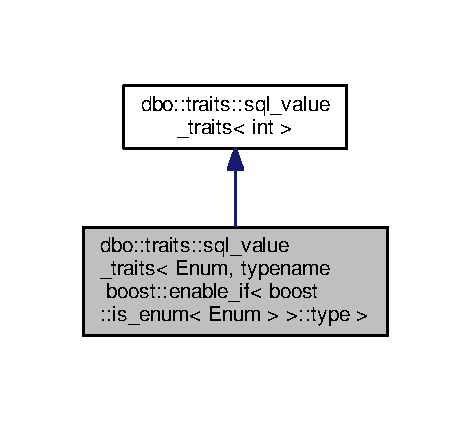
\includegraphics[width=226pt]{structdbo_1_1traits_1_1sql__value__traits_3_01_enum_00_01typename_01boost_1_1enable__if_3_01boos5008ffd71af7aaf3ac0f46b1624c2b91}
\end{center}
\end{figure}


Collaboration diagram for dbo\+:\+:traits\+:\+:sql\+\_\+value\+\_\+traits$<$ Enum, typename boost\+:\+:enable\+\_\+if$<$ boost\+:\+:is\+\_\+enum$<$ Enum $>$ $>$\+:\+:type $>$\+:\nopagebreak
\begin{figure}[H]
\begin{center}
\leavevmode
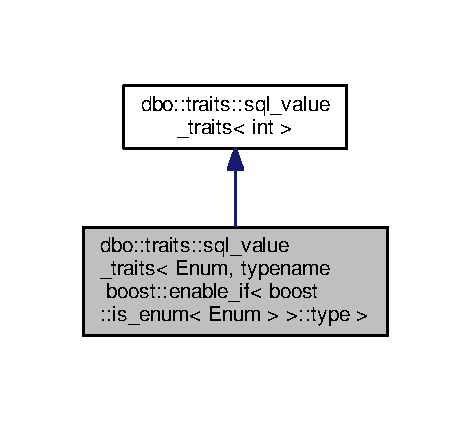
\includegraphics[width=226pt]{structdbo_1_1traits_1_1sql__value__traits_3_01_enum_00_01typename_01boost_1_1enable__if_3_01boosb09fed6fc036a161d753d0ad3ec76c32}
\end{center}
\end{figure}
\subsection*{Static Public Member Functions}
\begin{DoxyCompactItemize}
\item 
static void \hyperlink{structdbo_1_1traits_1_1sql__value__traits_3_01_enum_00_01typename_01boost_1_1enable__if_3_01boosf3db7d431a3cc6684d99d55c76c69c74_a36aa66ecb75b33e4e2188a92e7dcb2aa}{bind} (Enum v, \hyperlink{classdbo_1_1stmt_1_1_statement}{stmt\+::\+Statement} \&statement, int size)
\item 
static bool \hyperlink{structdbo_1_1traits_1_1sql__value__traits_3_01_enum_00_01typename_01boost_1_1enable__if_3_01boosf3db7d431a3cc6684d99d55c76c69c74_ad90a9efb8622c9e5bfa3e1336f2c4891}{read} (Enum \&v, \hyperlink{classdbo_1_1stmt_1_1_statement}{stmt\+::\+Statement} \&statement, int size)
\end{DoxyCompactItemize}
\subsection*{Additional Inherited Members}


\subsection{Member Function Documentation}
\hypertarget{structdbo_1_1traits_1_1sql__value__traits_3_01_enum_00_01typename_01boost_1_1enable__if_3_01boosf3db7d431a3cc6684d99d55c76c69c74_a36aa66ecb75b33e4e2188a92e7dcb2aa}{\index{dbo\+::traits\+::sql\+\_\+value\+\_\+traits$<$ Enum, typename boost\+::enable\+\_\+if$<$ boost\+::is\+\_\+enum$<$ Enum $>$ $>$\+::type $>$@{dbo\+::traits\+::sql\+\_\+value\+\_\+traits$<$ Enum, typename boost\+::enable\+\_\+if$<$ boost\+::is\+\_\+enum$<$ Enum $>$ $>$\+::type $>$}!bind@{bind}}
\index{bind@{bind}!dbo\+::traits\+::sql\+\_\+value\+\_\+traits$<$ Enum, typename boost\+::enable\+\_\+if$<$ boost\+::is\+\_\+enum$<$ Enum $>$ $>$\+::type $>$@{dbo\+::traits\+::sql\+\_\+value\+\_\+traits$<$ Enum, typename boost\+::enable\+\_\+if$<$ boost\+::is\+\_\+enum$<$ Enum $>$ $>$\+::type $>$}}
\subsubsection[{bind}]{\setlength{\rightskip}{0pt plus 5cm}template$<$typename Enum $>$ static void {\bf dbo\+::traits\+::sql\+\_\+value\+\_\+traits}$<$ Enum, typename boost\+::enable\+\_\+if$<$ boost\+::is\+\_\+enum$<$ Enum $>$ $>$\+::type $>$\+::bind (
\begin{DoxyParamCaption}
\item[{Enum}]{v, }
\item[{{\bf stmt\+::\+Statement} \&}]{statement, }
\item[{int}]{size}
\end{DoxyParamCaption}
)\hspace{0.3cm}{\ttfamily [inline]}, {\ttfamily [static]}}}\label{structdbo_1_1traits_1_1sql__value__traits_3_01_enum_00_01typename_01boost_1_1enable__if_3_01boosf3db7d431a3cc6684d99d55c76c69c74_a36aa66ecb75b33e4e2188a92e7dcb2aa}
\hypertarget{structdbo_1_1traits_1_1sql__value__traits_3_01_enum_00_01typename_01boost_1_1enable__if_3_01boosf3db7d431a3cc6684d99d55c76c69c74_ad90a9efb8622c9e5bfa3e1336f2c4891}{\index{dbo\+::traits\+::sql\+\_\+value\+\_\+traits$<$ Enum, typename boost\+::enable\+\_\+if$<$ boost\+::is\+\_\+enum$<$ Enum $>$ $>$\+::type $>$@{dbo\+::traits\+::sql\+\_\+value\+\_\+traits$<$ Enum, typename boost\+::enable\+\_\+if$<$ boost\+::is\+\_\+enum$<$ Enum $>$ $>$\+::type $>$}!read@{read}}
\index{read@{read}!dbo\+::traits\+::sql\+\_\+value\+\_\+traits$<$ Enum, typename boost\+::enable\+\_\+if$<$ boost\+::is\+\_\+enum$<$ Enum $>$ $>$\+::type $>$@{dbo\+::traits\+::sql\+\_\+value\+\_\+traits$<$ Enum, typename boost\+::enable\+\_\+if$<$ boost\+::is\+\_\+enum$<$ Enum $>$ $>$\+::type $>$}}
\subsubsection[{read}]{\setlength{\rightskip}{0pt plus 5cm}template$<$typename Enum $>$ static bool {\bf dbo\+::traits\+::sql\+\_\+value\+\_\+traits}$<$ Enum, typename boost\+::enable\+\_\+if$<$ boost\+::is\+\_\+enum$<$ Enum $>$ $>$\+::type $>$\+::read (
\begin{DoxyParamCaption}
\item[{Enum \&}]{v, }
\item[{{\bf stmt\+::\+Statement} \&}]{statement, }
\item[{int}]{size}
\end{DoxyParamCaption}
)\hspace{0.3cm}{\ttfamily [inline]}, {\ttfamily [static]}}}\label{structdbo_1_1traits_1_1sql__value__traits_3_01_enum_00_01typename_01boost_1_1enable__if_3_01boosf3db7d431a3cc6684d99d55c76c69c74_ad90a9efb8622c9e5bfa3e1336f2c4891}


The documentation for this struct was generated from the following file\+:\begin{DoxyCompactItemize}
\item 
dbo/traits/\hyperlink{_std_sql_traits_8h}{Std\+Sql\+Traits.\+h}\end{DoxyCompactItemize}

\hypertarget{structdbo_1_1traits_1_1sql__value__traits_3_01float_00_01void_01_4}{\section{dbo\+:\+:traits\+:\+:sql\+\_\+value\+\_\+traits$<$ float, void $>$ Struct Template Reference}
\label{structdbo_1_1traits_1_1sql__value__traits_3_01float_00_01void_01_4}\index{dbo\+::traits\+::sql\+\_\+value\+\_\+traits$<$ float, void $>$@{dbo\+::traits\+::sql\+\_\+value\+\_\+traits$<$ float, void $>$}}
}


{\ttfamily \#include $<$Std\+Sql\+Traits.\+h$>$}

\subsection*{Static Public Member Functions}
\begin{DoxyCompactItemize}
\item 
static std\+::string \hyperlink{structdbo_1_1traits_1_1sql__value__traits_3_01float_00_01void_01_4_af331ec88fbc0a93ea643b557b85996ea}{type} (int size)
\item 
static void \hyperlink{structdbo_1_1traits_1_1sql__value__traits_3_01float_00_01void_01_4_a4df8b2992a899fe00a71d4f5e7e4042d}{bind} (float v, \hyperlink{classdbo_1_1stmt_1_1_statement}{stmt\+::\+Statement} \&statement, int size)
\item 
static bool \hyperlink{structdbo_1_1traits_1_1sql__value__traits_3_01float_00_01void_01_4_a7366ecad146b0eae901f34fff9973dd6}{read} (float \&v, \hyperlink{classdbo_1_1stmt_1_1_statement}{stmt\+::\+Statement} \&statement, int size)
\end{DoxyCompactItemize}
\subsection*{Static Public Attributes}
\begin{DoxyCompactItemize}
\item 
static const bool \hyperlink{structdbo_1_1traits_1_1sql__value__traits_3_01float_00_01void_01_4_a9b693411503d1b7930349db153342216}{specialized} =true
\end{DoxyCompactItemize}


\subsection{Member Function Documentation}
\hypertarget{structdbo_1_1traits_1_1sql__value__traits_3_01float_00_01void_01_4_a4df8b2992a899fe00a71d4f5e7e4042d}{\index{dbo\+::traits\+::sql\+\_\+value\+\_\+traits$<$ float, void $>$@{dbo\+::traits\+::sql\+\_\+value\+\_\+traits$<$ float, void $>$}!bind@{bind}}
\index{bind@{bind}!dbo\+::traits\+::sql\+\_\+value\+\_\+traits$<$ float, void $>$@{dbo\+::traits\+::sql\+\_\+value\+\_\+traits$<$ float, void $>$}}
\subsubsection[{bind}]{\setlength{\rightskip}{0pt plus 5cm}static void {\bf dbo\+::traits\+::sql\+\_\+value\+\_\+traits}$<$ float, void $>$\+::bind (
\begin{DoxyParamCaption}
\item[{float}]{v, }
\item[{{\bf stmt\+::\+Statement} \&}]{statement, }
\item[{int}]{size}
\end{DoxyParamCaption}
)\hspace{0.3cm}{\ttfamily [static]}}}\label{structdbo_1_1traits_1_1sql__value__traits_3_01float_00_01void_01_4_a4df8b2992a899fe00a71d4f5e7e4042d}
\hypertarget{structdbo_1_1traits_1_1sql__value__traits_3_01float_00_01void_01_4_a7366ecad146b0eae901f34fff9973dd6}{\index{dbo\+::traits\+::sql\+\_\+value\+\_\+traits$<$ float, void $>$@{dbo\+::traits\+::sql\+\_\+value\+\_\+traits$<$ float, void $>$}!read@{read}}
\index{read@{read}!dbo\+::traits\+::sql\+\_\+value\+\_\+traits$<$ float, void $>$@{dbo\+::traits\+::sql\+\_\+value\+\_\+traits$<$ float, void $>$}}
\subsubsection[{read}]{\setlength{\rightskip}{0pt plus 5cm}static bool {\bf dbo\+::traits\+::sql\+\_\+value\+\_\+traits}$<$ float, void $>$\+::read (
\begin{DoxyParamCaption}
\item[{float \&}]{v, }
\item[{{\bf stmt\+::\+Statement} \&}]{statement, }
\item[{int}]{size}
\end{DoxyParamCaption}
)\hspace{0.3cm}{\ttfamily [static]}}}\label{structdbo_1_1traits_1_1sql__value__traits_3_01float_00_01void_01_4_a7366ecad146b0eae901f34fff9973dd6}
\hypertarget{structdbo_1_1traits_1_1sql__value__traits_3_01float_00_01void_01_4_af331ec88fbc0a93ea643b557b85996ea}{\index{dbo\+::traits\+::sql\+\_\+value\+\_\+traits$<$ float, void $>$@{dbo\+::traits\+::sql\+\_\+value\+\_\+traits$<$ float, void $>$}!type@{type}}
\index{type@{type}!dbo\+::traits\+::sql\+\_\+value\+\_\+traits$<$ float, void $>$@{dbo\+::traits\+::sql\+\_\+value\+\_\+traits$<$ float, void $>$}}
\subsubsection[{type}]{\setlength{\rightskip}{0pt plus 5cm}static std\+::string {\bf dbo\+::traits\+::sql\+\_\+value\+\_\+traits}$<$ float, void $>$\+::type (
\begin{DoxyParamCaption}
\item[{int}]{size}
\end{DoxyParamCaption}
)\hspace{0.3cm}{\ttfamily [static]}}}\label{structdbo_1_1traits_1_1sql__value__traits_3_01float_00_01void_01_4_af331ec88fbc0a93ea643b557b85996ea}


\subsection{Member Data Documentation}
\hypertarget{structdbo_1_1traits_1_1sql__value__traits_3_01float_00_01void_01_4_a9b693411503d1b7930349db153342216}{\index{dbo\+::traits\+::sql\+\_\+value\+\_\+traits$<$ float, void $>$@{dbo\+::traits\+::sql\+\_\+value\+\_\+traits$<$ float, void $>$}!specialized@{specialized}}
\index{specialized@{specialized}!dbo\+::traits\+::sql\+\_\+value\+\_\+traits$<$ float, void $>$@{dbo\+::traits\+::sql\+\_\+value\+\_\+traits$<$ float, void $>$}}
\subsubsection[{specialized}]{\setlength{\rightskip}{0pt plus 5cm}const bool {\bf dbo\+::traits\+::sql\+\_\+value\+\_\+traits}$<$ float, void $>$\+::specialized =true\hspace{0.3cm}{\ttfamily [static]}}}\label{structdbo_1_1traits_1_1sql__value__traits_3_01float_00_01void_01_4_a9b693411503d1b7930349db153342216}


The documentation for this struct was generated from the following file\+:\begin{DoxyCompactItemize}
\item 
dbo/traits/\hyperlink{_std_sql_traits_8h}{Std\+Sql\+Traits.\+h}\end{DoxyCompactItemize}

\hypertarget{structdbo_1_1traits_1_1sql__value__traits_3_01int_00_01void_01_4}{\section{dbo\+:\+:traits\+:\+:sql\+\_\+value\+\_\+traits$<$ int, void $>$ Struct Template Reference}
\label{structdbo_1_1traits_1_1sql__value__traits_3_01int_00_01void_01_4}\index{dbo\+::traits\+::sql\+\_\+value\+\_\+traits$<$ int, void $>$@{dbo\+::traits\+::sql\+\_\+value\+\_\+traits$<$ int, void $>$}}
}


{\ttfamily \#include $<$Std\+Sql\+Traits.\+h$>$}

\subsection*{Static Public Member Functions}
\begin{DoxyCompactItemize}
\item 
static std\+::string \hyperlink{structdbo_1_1traits_1_1sql__value__traits_3_01int_00_01void_01_4_ac31d760d1acdf026409e92111e061e82}{type} (int size)
\item 
static void \hyperlink{structdbo_1_1traits_1_1sql__value__traits_3_01int_00_01void_01_4_aec351dcb72702b01ac0b1ceead67b519}{bind} (int v, \hyperlink{classdbo_1_1stmt_1_1_statement}{stmt\+::\+Statement} \&statement, int size)
\item 
static bool \hyperlink{structdbo_1_1traits_1_1sql__value__traits_3_01int_00_01void_01_4_a300457ce6a904ba6f17cffe6f71c78be}{read} (int \&v, \hyperlink{classdbo_1_1stmt_1_1_statement}{stmt\+::\+Statement} \&statement, int size)
\end{DoxyCompactItemize}
\subsection*{Static Public Attributes}
\begin{DoxyCompactItemize}
\item 
static const bool \hyperlink{structdbo_1_1traits_1_1sql__value__traits_3_01int_00_01void_01_4_a1b5a328dcfb4c559cb023133c073c090}{specialized} =true
\end{DoxyCompactItemize}


\subsection{Member Function Documentation}
\hypertarget{structdbo_1_1traits_1_1sql__value__traits_3_01int_00_01void_01_4_aec351dcb72702b01ac0b1ceead67b519}{\index{dbo\+::traits\+::sql\+\_\+value\+\_\+traits$<$ int, void $>$@{dbo\+::traits\+::sql\+\_\+value\+\_\+traits$<$ int, void $>$}!bind@{bind}}
\index{bind@{bind}!dbo\+::traits\+::sql\+\_\+value\+\_\+traits$<$ int, void $>$@{dbo\+::traits\+::sql\+\_\+value\+\_\+traits$<$ int, void $>$}}
\subsubsection[{bind}]{\setlength{\rightskip}{0pt plus 5cm}static void {\bf dbo\+::traits\+::sql\+\_\+value\+\_\+traits}$<$ int, void $>$\+::bind (
\begin{DoxyParamCaption}
\item[{int}]{v, }
\item[{{\bf stmt\+::\+Statement} \&}]{statement, }
\item[{int}]{size}
\end{DoxyParamCaption}
)\hspace{0.3cm}{\ttfamily [static]}}}\label{structdbo_1_1traits_1_1sql__value__traits_3_01int_00_01void_01_4_aec351dcb72702b01ac0b1ceead67b519}
\hypertarget{structdbo_1_1traits_1_1sql__value__traits_3_01int_00_01void_01_4_a300457ce6a904ba6f17cffe6f71c78be}{\index{dbo\+::traits\+::sql\+\_\+value\+\_\+traits$<$ int, void $>$@{dbo\+::traits\+::sql\+\_\+value\+\_\+traits$<$ int, void $>$}!read@{read}}
\index{read@{read}!dbo\+::traits\+::sql\+\_\+value\+\_\+traits$<$ int, void $>$@{dbo\+::traits\+::sql\+\_\+value\+\_\+traits$<$ int, void $>$}}
\subsubsection[{read}]{\setlength{\rightskip}{0pt plus 5cm}static bool {\bf dbo\+::traits\+::sql\+\_\+value\+\_\+traits}$<$ int, void $>$\+::read (
\begin{DoxyParamCaption}
\item[{int \&}]{v, }
\item[{{\bf stmt\+::\+Statement} \&}]{statement, }
\item[{int}]{size}
\end{DoxyParamCaption}
)\hspace{0.3cm}{\ttfamily [static]}}}\label{structdbo_1_1traits_1_1sql__value__traits_3_01int_00_01void_01_4_a300457ce6a904ba6f17cffe6f71c78be}
\hypertarget{structdbo_1_1traits_1_1sql__value__traits_3_01int_00_01void_01_4_ac31d760d1acdf026409e92111e061e82}{\index{dbo\+::traits\+::sql\+\_\+value\+\_\+traits$<$ int, void $>$@{dbo\+::traits\+::sql\+\_\+value\+\_\+traits$<$ int, void $>$}!type@{type}}
\index{type@{type}!dbo\+::traits\+::sql\+\_\+value\+\_\+traits$<$ int, void $>$@{dbo\+::traits\+::sql\+\_\+value\+\_\+traits$<$ int, void $>$}}
\subsubsection[{type}]{\setlength{\rightskip}{0pt plus 5cm}static std\+::string {\bf dbo\+::traits\+::sql\+\_\+value\+\_\+traits}$<$ int, void $>$\+::type (
\begin{DoxyParamCaption}
\item[{int}]{size}
\end{DoxyParamCaption}
)\hspace{0.3cm}{\ttfamily [static]}}}\label{structdbo_1_1traits_1_1sql__value__traits_3_01int_00_01void_01_4_ac31d760d1acdf026409e92111e061e82}


\subsection{Member Data Documentation}
\hypertarget{structdbo_1_1traits_1_1sql__value__traits_3_01int_00_01void_01_4_a1b5a328dcfb4c559cb023133c073c090}{\index{dbo\+::traits\+::sql\+\_\+value\+\_\+traits$<$ int, void $>$@{dbo\+::traits\+::sql\+\_\+value\+\_\+traits$<$ int, void $>$}!specialized@{specialized}}
\index{specialized@{specialized}!dbo\+::traits\+::sql\+\_\+value\+\_\+traits$<$ int, void $>$@{dbo\+::traits\+::sql\+\_\+value\+\_\+traits$<$ int, void $>$}}
\subsubsection[{specialized}]{\setlength{\rightskip}{0pt plus 5cm}const bool {\bf dbo\+::traits\+::sql\+\_\+value\+\_\+traits}$<$ int, void $>$\+::specialized =true\hspace{0.3cm}{\ttfamily [static]}}}\label{structdbo_1_1traits_1_1sql__value__traits_3_01int_00_01void_01_4_a1b5a328dcfb4c559cb023133c073c090}


The documentation for this struct was generated from the following file\+:\begin{DoxyCompactItemize}
\item 
dbo/traits/\hyperlink{_std_sql_traits_8h}{Std\+Sql\+Traits.\+h}\end{DoxyCompactItemize}

\hypertarget{structdbo_1_1traits_1_1sql__value__traits_3_01long_01long_00_01void_01_4}{\section{dbo\+:\+:traits\+:\+:sql\+\_\+value\+\_\+traits$<$ long long, void $>$ Struct Template Reference}
\label{structdbo_1_1traits_1_1sql__value__traits_3_01long_01long_00_01void_01_4}\index{dbo\+::traits\+::sql\+\_\+value\+\_\+traits$<$ long long, void $>$@{dbo\+::traits\+::sql\+\_\+value\+\_\+traits$<$ long long, void $>$}}
}


{\ttfamily \#include $<$Std\+Sql\+Traits.\+h$>$}

\subsection*{Static Public Member Functions}
\begin{DoxyCompactItemize}
\item 
static std\+::string \hyperlink{structdbo_1_1traits_1_1sql__value__traits_3_01long_01long_00_01void_01_4_a882c441114bc8d5367678498486bb406}{type} (int size)
\item 
static void \hyperlink{structdbo_1_1traits_1_1sql__value__traits_3_01long_01long_00_01void_01_4_a17e9403175dc6e4dd31d6ef6925e6053}{bind} (long long v, \hyperlink{classdbo_1_1stmt_1_1_statement}{stmt\+::\+Statement} \&statement, int size)
\item 
static bool \hyperlink{structdbo_1_1traits_1_1sql__value__traits_3_01long_01long_00_01void_01_4_a83ba40b8ab09959896bd7d4746e0f8ae}{read} (long long \&v, \hyperlink{classdbo_1_1stmt_1_1_statement}{stmt\+::\+Statement} \&statement, int size)
\end{DoxyCompactItemize}
\subsection*{Static Public Attributes}
\begin{DoxyCompactItemize}
\item 
static const bool \hyperlink{structdbo_1_1traits_1_1sql__value__traits_3_01long_01long_00_01void_01_4_ad9092faa08a6e0fab84acb9fe2c4ba7a}{specialized} =true
\end{DoxyCompactItemize}


\subsection{Member Function Documentation}
\hypertarget{structdbo_1_1traits_1_1sql__value__traits_3_01long_01long_00_01void_01_4_a17e9403175dc6e4dd31d6ef6925e6053}{\index{dbo\+::traits\+::sql\+\_\+value\+\_\+traits$<$ long long, void $>$@{dbo\+::traits\+::sql\+\_\+value\+\_\+traits$<$ long long, void $>$}!bind@{bind}}
\index{bind@{bind}!dbo\+::traits\+::sql\+\_\+value\+\_\+traits$<$ long long, void $>$@{dbo\+::traits\+::sql\+\_\+value\+\_\+traits$<$ long long, void $>$}}
\subsubsection[{bind}]{\setlength{\rightskip}{0pt plus 5cm}static void {\bf dbo\+::traits\+::sql\+\_\+value\+\_\+traits}$<$ long long, void $>$\+::bind (
\begin{DoxyParamCaption}
\item[{long long}]{v, }
\item[{{\bf stmt\+::\+Statement} \&}]{statement, }
\item[{int}]{size}
\end{DoxyParamCaption}
)\hspace{0.3cm}{\ttfamily [static]}}}\label{structdbo_1_1traits_1_1sql__value__traits_3_01long_01long_00_01void_01_4_a17e9403175dc6e4dd31d6ef6925e6053}
\hypertarget{structdbo_1_1traits_1_1sql__value__traits_3_01long_01long_00_01void_01_4_a83ba40b8ab09959896bd7d4746e0f8ae}{\index{dbo\+::traits\+::sql\+\_\+value\+\_\+traits$<$ long long, void $>$@{dbo\+::traits\+::sql\+\_\+value\+\_\+traits$<$ long long, void $>$}!read@{read}}
\index{read@{read}!dbo\+::traits\+::sql\+\_\+value\+\_\+traits$<$ long long, void $>$@{dbo\+::traits\+::sql\+\_\+value\+\_\+traits$<$ long long, void $>$}}
\subsubsection[{read}]{\setlength{\rightskip}{0pt plus 5cm}static bool {\bf dbo\+::traits\+::sql\+\_\+value\+\_\+traits}$<$ long long, void $>$\+::read (
\begin{DoxyParamCaption}
\item[{long long \&}]{v, }
\item[{{\bf stmt\+::\+Statement} \&}]{statement, }
\item[{int}]{size}
\end{DoxyParamCaption}
)\hspace{0.3cm}{\ttfamily [static]}}}\label{structdbo_1_1traits_1_1sql__value__traits_3_01long_01long_00_01void_01_4_a83ba40b8ab09959896bd7d4746e0f8ae}
\hypertarget{structdbo_1_1traits_1_1sql__value__traits_3_01long_01long_00_01void_01_4_a882c441114bc8d5367678498486bb406}{\index{dbo\+::traits\+::sql\+\_\+value\+\_\+traits$<$ long long, void $>$@{dbo\+::traits\+::sql\+\_\+value\+\_\+traits$<$ long long, void $>$}!type@{type}}
\index{type@{type}!dbo\+::traits\+::sql\+\_\+value\+\_\+traits$<$ long long, void $>$@{dbo\+::traits\+::sql\+\_\+value\+\_\+traits$<$ long long, void $>$}}
\subsubsection[{type}]{\setlength{\rightskip}{0pt plus 5cm}static std\+::string {\bf dbo\+::traits\+::sql\+\_\+value\+\_\+traits}$<$ long long, void $>$\+::type (
\begin{DoxyParamCaption}
\item[{int}]{size}
\end{DoxyParamCaption}
)\hspace{0.3cm}{\ttfamily [static]}}}\label{structdbo_1_1traits_1_1sql__value__traits_3_01long_01long_00_01void_01_4_a882c441114bc8d5367678498486bb406}


\subsection{Member Data Documentation}
\hypertarget{structdbo_1_1traits_1_1sql__value__traits_3_01long_01long_00_01void_01_4_ad9092faa08a6e0fab84acb9fe2c4ba7a}{\index{dbo\+::traits\+::sql\+\_\+value\+\_\+traits$<$ long long, void $>$@{dbo\+::traits\+::sql\+\_\+value\+\_\+traits$<$ long long, void $>$}!specialized@{specialized}}
\index{specialized@{specialized}!dbo\+::traits\+::sql\+\_\+value\+\_\+traits$<$ long long, void $>$@{dbo\+::traits\+::sql\+\_\+value\+\_\+traits$<$ long long, void $>$}}
\subsubsection[{specialized}]{\setlength{\rightskip}{0pt plus 5cm}const bool {\bf dbo\+::traits\+::sql\+\_\+value\+\_\+traits}$<$ long long, void $>$\+::specialized =true\hspace{0.3cm}{\ttfamily [static]}}}\label{structdbo_1_1traits_1_1sql__value__traits_3_01long_01long_00_01void_01_4_ad9092faa08a6e0fab84acb9fe2c4ba7a}


The documentation for this struct was generated from the following file\+:\begin{DoxyCompactItemize}
\item 
dbo/traits/\hyperlink{_std_sql_traits_8h}{Std\+Sql\+Traits.\+h}\end{DoxyCompactItemize}

\hypertarget{structdbo_1_1traits_1_1sql__value__traits_3_01long_00_01void_01_4}{\section{dbo\+:\+:traits\+:\+:sql\+\_\+value\+\_\+traits$<$ long, void $>$ Struct Template Reference}
\label{structdbo_1_1traits_1_1sql__value__traits_3_01long_00_01void_01_4}\index{dbo\+::traits\+::sql\+\_\+value\+\_\+traits$<$ long, void $>$@{dbo\+::traits\+::sql\+\_\+value\+\_\+traits$<$ long, void $>$}}
}


{\ttfamily \#include $<$Std\+Sql\+Traits.\+h$>$}

\subsection*{Static Public Member Functions}
\begin{DoxyCompactItemize}
\item 
static std\+::string \hyperlink{structdbo_1_1traits_1_1sql__value__traits_3_01long_00_01void_01_4_a45c06ff3f1562386293a5fc953a458f2}{type} (int size)
\item 
static void \hyperlink{structdbo_1_1traits_1_1sql__value__traits_3_01long_00_01void_01_4_a0e20de466f7716d430ecdf55a1bfb345}{bind} (long v, \hyperlink{classdbo_1_1stmt_1_1_statement}{stmt\+::\+Statement} \&statement, int size)
\item 
static bool \hyperlink{structdbo_1_1traits_1_1sql__value__traits_3_01long_00_01void_01_4_a6ecadd57f3d8bdf025028bcb3be9d048}{read} (long \&v, \hyperlink{classdbo_1_1stmt_1_1_statement}{stmt\+::\+Statement} \&statement, int size)
\end{DoxyCompactItemize}
\subsection*{Static Public Attributes}
\begin{DoxyCompactItemize}
\item 
static const bool \hyperlink{structdbo_1_1traits_1_1sql__value__traits_3_01long_00_01void_01_4_a5cdf7ca5fefd9b06e2afff8c1f981cd4}{specialized} =true
\end{DoxyCompactItemize}


\subsection{Member Function Documentation}
\hypertarget{structdbo_1_1traits_1_1sql__value__traits_3_01long_00_01void_01_4_a0e20de466f7716d430ecdf55a1bfb345}{\index{dbo\+::traits\+::sql\+\_\+value\+\_\+traits$<$ long, void $>$@{dbo\+::traits\+::sql\+\_\+value\+\_\+traits$<$ long, void $>$}!bind@{bind}}
\index{bind@{bind}!dbo\+::traits\+::sql\+\_\+value\+\_\+traits$<$ long, void $>$@{dbo\+::traits\+::sql\+\_\+value\+\_\+traits$<$ long, void $>$}}
\subsubsection[{bind}]{\setlength{\rightskip}{0pt plus 5cm}static void {\bf dbo\+::traits\+::sql\+\_\+value\+\_\+traits}$<$ long, void $>$\+::bind (
\begin{DoxyParamCaption}
\item[{long}]{v, }
\item[{{\bf stmt\+::\+Statement} \&}]{statement, }
\item[{int}]{size}
\end{DoxyParamCaption}
)\hspace{0.3cm}{\ttfamily [static]}}}\label{structdbo_1_1traits_1_1sql__value__traits_3_01long_00_01void_01_4_a0e20de466f7716d430ecdf55a1bfb345}
\hypertarget{structdbo_1_1traits_1_1sql__value__traits_3_01long_00_01void_01_4_a6ecadd57f3d8bdf025028bcb3be9d048}{\index{dbo\+::traits\+::sql\+\_\+value\+\_\+traits$<$ long, void $>$@{dbo\+::traits\+::sql\+\_\+value\+\_\+traits$<$ long, void $>$}!read@{read}}
\index{read@{read}!dbo\+::traits\+::sql\+\_\+value\+\_\+traits$<$ long, void $>$@{dbo\+::traits\+::sql\+\_\+value\+\_\+traits$<$ long, void $>$}}
\subsubsection[{read}]{\setlength{\rightskip}{0pt plus 5cm}static bool {\bf dbo\+::traits\+::sql\+\_\+value\+\_\+traits}$<$ long, void $>$\+::read (
\begin{DoxyParamCaption}
\item[{long \&}]{v, }
\item[{{\bf stmt\+::\+Statement} \&}]{statement, }
\item[{int}]{size}
\end{DoxyParamCaption}
)\hspace{0.3cm}{\ttfamily [static]}}}\label{structdbo_1_1traits_1_1sql__value__traits_3_01long_00_01void_01_4_a6ecadd57f3d8bdf025028bcb3be9d048}
\hypertarget{structdbo_1_1traits_1_1sql__value__traits_3_01long_00_01void_01_4_a45c06ff3f1562386293a5fc953a458f2}{\index{dbo\+::traits\+::sql\+\_\+value\+\_\+traits$<$ long, void $>$@{dbo\+::traits\+::sql\+\_\+value\+\_\+traits$<$ long, void $>$}!type@{type}}
\index{type@{type}!dbo\+::traits\+::sql\+\_\+value\+\_\+traits$<$ long, void $>$@{dbo\+::traits\+::sql\+\_\+value\+\_\+traits$<$ long, void $>$}}
\subsubsection[{type}]{\setlength{\rightskip}{0pt plus 5cm}static std\+::string {\bf dbo\+::traits\+::sql\+\_\+value\+\_\+traits}$<$ long, void $>$\+::type (
\begin{DoxyParamCaption}
\item[{int}]{size}
\end{DoxyParamCaption}
)\hspace{0.3cm}{\ttfamily [static]}}}\label{structdbo_1_1traits_1_1sql__value__traits_3_01long_00_01void_01_4_a45c06ff3f1562386293a5fc953a458f2}


\subsection{Member Data Documentation}
\hypertarget{structdbo_1_1traits_1_1sql__value__traits_3_01long_00_01void_01_4_a5cdf7ca5fefd9b06e2afff8c1f981cd4}{\index{dbo\+::traits\+::sql\+\_\+value\+\_\+traits$<$ long, void $>$@{dbo\+::traits\+::sql\+\_\+value\+\_\+traits$<$ long, void $>$}!specialized@{specialized}}
\index{specialized@{specialized}!dbo\+::traits\+::sql\+\_\+value\+\_\+traits$<$ long, void $>$@{dbo\+::traits\+::sql\+\_\+value\+\_\+traits$<$ long, void $>$}}
\subsubsection[{specialized}]{\setlength{\rightskip}{0pt plus 5cm}const bool {\bf dbo\+::traits\+::sql\+\_\+value\+\_\+traits}$<$ long, void $>$\+::specialized =true\hspace{0.3cm}{\ttfamily [static]}}}\label{structdbo_1_1traits_1_1sql__value__traits_3_01long_00_01void_01_4_a5cdf7ca5fefd9b06e2afff8c1f981cd4}


The documentation for this struct was generated from the following file\+:\begin{DoxyCompactItemize}
\item 
dbo/traits/\hyperlink{_std_sql_traits_8h}{Std\+Sql\+Traits.\+h}\end{DoxyCompactItemize}

\hypertarget{structdbo_1_1traits_1_1sql__value__traits_3_01short_00_01void_01_4}{\section{dbo\+:\+:traits\+:\+:sql\+\_\+value\+\_\+traits$<$ short, void $>$ Struct Template Reference}
\label{structdbo_1_1traits_1_1sql__value__traits_3_01short_00_01void_01_4}\index{dbo\+::traits\+::sql\+\_\+value\+\_\+traits$<$ short, void $>$@{dbo\+::traits\+::sql\+\_\+value\+\_\+traits$<$ short, void $>$}}
}


{\ttfamily \#include $<$Std\+Sql\+Traits.\+h$>$}

\subsection*{Static Public Member Functions}
\begin{DoxyCompactItemize}
\item 
static std\+::string \hyperlink{structdbo_1_1traits_1_1sql__value__traits_3_01short_00_01void_01_4_ac57b46adba46d6e1f8425dd43b1b2cec}{type} (int size)
\item 
static void \hyperlink{structdbo_1_1traits_1_1sql__value__traits_3_01short_00_01void_01_4_a4979e764123d914551319444ab8e4cc1}{bind} (short v, \hyperlink{classdbo_1_1stmt_1_1_statement}{stmt\+::\+Statement} \&statement, int size)
\item 
static bool \hyperlink{structdbo_1_1traits_1_1sql__value__traits_3_01short_00_01void_01_4_a18b5c5a2243ebb84a9fe874d91f1ac4d}{read} (short \&v, \hyperlink{classdbo_1_1stmt_1_1_statement}{stmt\+::\+Statement} \&statement, int size)
\end{DoxyCompactItemize}
\subsection*{Static Public Attributes}
\begin{DoxyCompactItemize}
\item 
static const bool \hyperlink{structdbo_1_1traits_1_1sql__value__traits_3_01short_00_01void_01_4_aff786ebbd2068ab6fc4ac329989c3ce6}{specialized} =true
\end{DoxyCompactItemize}


\subsection{Member Function Documentation}
\hypertarget{structdbo_1_1traits_1_1sql__value__traits_3_01short_00_01void_01_4_a4979e764123d914551319444ab8e4cc1}{\index{dbo\+::traits\+::sql\+\_\+value\+\_\+traits$<$ short, void $>$@{dbo\+::traits\+::sql\+\_\+value\+\_\+traits$<$ short, void $>$}!bind@{bind}}
\index{bind@{bind}!dbo\+::traits\+::sql\+\_\+value\+\_\+traits$<$ short, void $>$@{dbo\+::traits\+::sql\+\_\+value\+\_\+traits$<$ short, void $>$}}
\subsubsection[{bind}]{\setlength{\rightskip}{0pt plus 5cm}static void {\bf dbo\+::traits\+::sql\+\_\+value\+\_\+traits}$<$ short, void $>$\+::bind (
\begin{DoxyParamCaption}
\item[{short}]{v, }
\item[{{\bf stmt\+::\+Statement} \&}]{statement, }
\item[{int}]{size}
\end{DoxyParamCaption}
)\hspace{0.3cm}{\ttfamily [static]}}}\label{structdbo_1_1traits_1_1sql__value__traits_3_01short_00_01void_01_4_a4979e764123d914551319444ab8e4cc1}
\hypertarget{structdbo_1_1traits_1_1sql__value__traits_3_01short_00_01void_01_4_a18b5c5a2243ebb84a9fe874d91f1ac4d}{\index{dbo\+::traits\+::sql\+\_\+value\+\_\+traits$<$ short, void $>$@{dbo\+::traits\+::sql\+\_\+value\+\_\+traits$<$ short, void $>$}!read@{read}}
\index{read@{read}!dbo\+::traits\+::sql\+\_\+value\+\_\+traits$<$ short, void $>$@{dbo\+::traits\+::sql\+\_\+value\+\_\+traits$<$ short, void $>$}}
\subsubsection[{read}]{\setlength{\rightskip}{0pt plus 5cm}static bool {\bf dbo\+::traits\+::sql\+\_\+value\+\_\+traits}$<$ short, void $>$\+::read (
\begin{DoxyParamCaption}
\item[{short \&}]{v, }
\item[{{\bf stmt\+::\+Statement} \&}]{statement, }
\item[{int}]{size}
\end{DoxyParamCaption}
)\hspace{0.3cm}{\ttfamily [static]}}}\label{structdbo_1_1traits_1_1sql__value__traits_3_01short_00_01void_01_4_a18b5c5a2243ebb84a9fe874d91f1ac4d}
\hypertarget{structdbo_1_1traits_1_1sql__value__traits_3_01short_00_01void_01_4_ac57b46adba46d6e1f8425dd43b1b2cec}{\index{dbo\+::traits\+::sql\+\_\+value\+\_\+traits$<$ short, void $>$@{dbo\+::traits\+::sql\+\_\+value\+\_\+traits$<$ short, void $>$}!type@{type}}
\index{type@{type}!dbo\+::traits\+::sql\+\_\+value\+\_\+traits$<$ short, void $>$@{dbo\+::traits\+::sql\+\_\+value\+\_\+traits$<$ short, void $>$}}
\subsubsection[{type}]{\setlength{\rightskip}{0pt plus 5cm}static std\+::string {\bf dbo\+::traits\+::sql\+\_\+value\+\_\+traits}$<$ short, void $>$\+::type (
\begin{DoxyParamCaption}
\item[{int}]{size}
\end{DoxyParamCaption}
)\hspace{0.3cm}{\ttfamily [static]}}}\label{structdbo_1_1traits_1_1sql__value__traits_3_01short_00_01void_01_4_ac57b46adba46d6e1f8425dd43b1b2cec}


\subsection{Member Data Documentation}
\hypertarget{structdbo_1_1traits_1_1sql__value__traits_3_01short_00_01void_01_4_aff786ebbd2068ab6fc4ac329989c3ce6}{\index{dbo\+::traits\+::sql\+\_\+value\+\_\+traits$<$ short, void $>$@{dbo\+::traits\+::sql\+\_\+value\+\_\+traits$<$ short, void $>$}!specialized@{specialized}}
\index{specialized@{specialized}!dbo\+::traits\+::sql\+\_\+value\+\_\+traits$<$ short, void $>$@{dbo\+::traits\+::sql\+\_\+value\+\_\+traits$<$ short, void $>$}}
\subsubsection[{specialized}]{\setlength{\rightskip}{0pt plus 5cm}const bool {\bf dbo\+::traits\+::sql\+\_\+value\+\_\+traits}$<$ short, void $>$\+::specialized =true\hspace{0.3cm}{\ttfamily [static]}}}\label{structdbo_1_1traits_1_1sql__value__traits_3_01short_00_01void_01_4_aff786ebbd2068ab6fc4ac329989c3ce6}


The documentation for this struct was generated from the following file\+:\begin{DoxyCompactItemize}
\item 
dbo/traits/\hyperlink{_std_sql_traits_8h}{Std\+Sql\+Traits.\+h}\end{DoxyCompactItemize}

\hypertarget{structdbo_1_1traits_1_1sql__value__traits_3_01size__t_00_01void_01_4}{\section{dbo\+:\+:traits\+:\+:sql\+\_\+value\+\_\+traits$<$ size\+\_\+t, void $>$ Struct Template Reference}
\label{structdbo_1_1traits_1_1sql__value__traits_3_01size__t_00_01void_01_4}\index{dbo\+::traits\+::sql\+\_\+value\+\_\+traits$<$ size\+\_\+t, void $>$@{dbo\+::traits\+::sql\+\_\+value\+\_\+traits$<$ size\+\_\+t, void $>$}}
}


{\ttfamily \#include $<$Std\+Sql\+Traits.\+h$>$}

\subsection*{Static Public Member Functions}
\begin{DoxyCompactItemize}
\item 
static std\+::string \hyperlink{structdbo_1_1traits_1_1sql__value__traits_3_01size__t_00_01void_01_4_ad75722a868b313ca32d695c34b366b4b}{type} (int size)
\item 
static void \hyperlink{structdbo_1_1traits_1_1sql__value__traits_3_01size__t_00_01void_01_4_a3e4ff80ea517b697c9404fe253c63466}{bind} (size\+\_\+t v, \hyperlink{classdbo_1_1stmt_1_1_statement}{stmt\+::\+Statement} \&statement, int size)
\item 
static bool \hyperlink{structdbo_1_1traits_1_1sql__value__traits_3_01size__t_00_01void_01_4_a1148f98b73c6733fa52dad05098f08ce}{read} (size\+\_\+t \&v, \hyperlink{classdbo_1_1stmt_1_1_statement}{stmt\+::\+Statement} \&statement, int size)
\end{DoxyCompactItemize}
\subsection*{Static Public Attributes}
\begin{DoxyCompactItemize}
\item 
static const bool \hyperlink{structdbo_1_1traits_1_1sql__value__traits_3_01size__t_00_01void_01_4_ae2e4a1d9acfdf62e18892b58a50b57d8}{specialized} =true
\end{DoxyCompactItemize}


\subsection{Member Function Documentation}
\hypertarget{structdbo_1_1traits_1_1sql__value__traits_3_01size__t_00_01void_01_4_a3e4ff80ea517b697c9404fe253c63466}{\index{dbo\+::traits\+::sql\+\_\+value\+\_\+traits$<$ size\+\_\+t, void $>$@{dbo\+::traits\+::sql\+\_\+value\+\_\+traits$<$ size\+\_\+t, void $>$}!bind@{bind}}
\index{bind@{bind}!dbo\+::traits\+::sql\+\_\+value\+\_\+traits$<$ size\+\_\+t, void $>$@{dbo\+::traits\+::sql\+\_\+value\+\_\+traits$<$ size\+\_\+t, void $>$}}
\subsubsection[{bind}]{\setlength{\rightskip}{0pt plus 5cm}static void {\bf dbo\+::traits\+::sql\+\_\+value\+\_\+traits}$<$ size\+\_\+t, void $>$\+::bind (
\begin{DoxyParamCaption}
\item[{size\+\_\+t}]{v, }
\item[{{\bf stmt\+::\+Statement} \&}]{statement, }
\item[{int}]{size}
\end{DoxyParamCaption}
)\hspace{0.3cm}{\ttfamily [static]}}}\label{structdbo_1_1traits_1_1sql__value__traits_3_01size__t_00_01void_01_4_a3e4ff80ea517b697c9404fe253c63466}
\hypertarget{structdbo_1_1traits_1_1sql__value__traits_3_01size__t_00_01void_01_4_a1148f98b73c6733fa52dad05098f08ce}{\index{dbo\+::traits\+::sql\+\_\+value\+\_\+traits$<$ size\+\_\+t, void $>$@{dbo\+::traits\+::sql\+\_\+value\+\_\+traits$<$ size\+\_\+t, void $>$}!read@{read}}
\index{read@{read}!dbo\+::traits\+::sql\+\_\+value\+\_\+traits$<$ size\+\_\+t, void $>$@{dbo\+::traits\+::sql\+\_\+value\+\_\+traits$<$ size\+\_\+t, void $>$}}
\subsubsection[{read}]{\setlength{\rightskip}{0pt plus 5cm}static bool {\bf dbo\+::traits\+::sql\+\_\+value\+\_\+traits}$<$ size\+\_\+t, void $>$\+::read (
\begin{DoxyParamCaption}
\item[{size\+\_\+t \&}]{v, }
\item[{{\bf stmt\+::\+Statement} \&}]{statement, }
\item[{int}]{size}
\end{DoxyParamCaption}
)\hspace{0.3cm}{\ttfamily [static]}}}\label{structdbo_1_1traits_1_1sql__value__traits_3_01size__t_00_01void_01_4_a1148f98b73c6733fa52dad05098f08ce}
\hypertarget{structdbo_1_1traits_1_1sql__value__traits_3_01size__t_00_01void_01_4_ad75722a868b313ca32d695c34b366b4b}{\index{dbo\+::traits\+::sql\+\_\+value\+\_\+traits$<$ size\+\_\+t, void $>$@{dbo\+::traits\+::sql\+\_\+value\+\_\+traits$<$ size\+\_\+t, void $>$}!type@{type}}
\index{type@{type}!dbo\+::traits\+::sql\+\_\+value\+\_\+traits$<$ size\+\_\+t, void $>$@{dbo\+::traits\+::sql\+\_\+value\+\_\+traits$<$ size\+\_\+t, void $>$}}
\subsubsection[{type}]{\setlength{\rightskip}{0pt plus 5cm}static std\+::string {\bf dbo\+::traits\+::sql\+\_\+value\+\_\+traits}$<$ size\+\_\+t, void $>$\+::type (
\begin{DoxyParamCaption}
\item[{int}]{size}
\end{DoxyParamCaption}
)\hspace{0.3cm}{\ttfamily [static]}}}\label{structdbo_1_1traits_1_1sql__value__traits_3_01size__t_00_01void_01_4_ad75722a868b313ca32d695c34b366b4b}


\subsection{Member Data Documentation}
\hypertarget{structdbo_1_1traits_1_1sql__value__traits_3_01size__t_00_01void_01_4_ae2e4a1d9acfdf62e18892b58a50b57d8}{\index{dbo\+::traits\+::sql\+\_\+value\+\_\+traits$<$ size\+\_\+t, void $>$@{dbo\+::traits\+::sql\+\_\+value\+\_\+traits$<$ size\+\_\+t, void $>$}!specialized@{specialized}}
\index{specialized@{specialized}!dbo\+::traits\+::sql\+\_\+value\+\_\+traits$<$ size\+\_\+t, void $>$@{dbo\+::traits\+::sql\+\_\+value\+\_\+traits$<$ size\+\_\+t, void $>$}}
\subsubsection[{specialized}]{\setlength{\rightskip}{0pt plus 5cm}const bool {\bf dbo\+::traits\+::sql\+\_\+value\+\_\+traits}$<$ size\+\_\+t, void $>$\+::specialized =true\hspace{0.3cm}{\ttfamily [static]}}}\label{structdbo_1_1traits_1_1sql__value__traits_3_01size__t_00_01void_01_4_ae2e4a1d9acfdf62e18892b58a50b57d8}


The documentation for this struct was generated from the following file\+:\begin{DoxyCompactItemize}
\item 
dbo/traits/\hyperlink{_std_sql_traits_8h}{Std\+Sql\+Traits.\+h}\end{DoxyCompactItemize}

\hypertarget{structdbo_1_1traits_1_1sql__value__traits_3_01std_1_1string_00_01void_01_4}{\section{dbo\+:\+:traits\+:\+:sql\+\_\+value\+\_\+traits$<$ std\+:\+:string, void $>$ Struct Template Reference}
\label{structdbo_1_1traits_1_1sql__value__traits_3_01std_1_1string_00_01void_01_4}\index{dbo\+::traits\+::sql\+\_\+value\+\_\+traits$<$ std\+::string, void $>$@{dbo\+::traits\+::sql\+\_\+value\+\_\+traits$<$ std\+::string, void $>$}}
}


{\ttfamily \#include $<$Std\+Sql\+Traits.\+h$>$}

\subsection*{Static Public Member Functions}
\begin{DoxyCompactItemize}
\item 
static std\+::string \hyperlink{structdbo_1_1traits_1_1sql__value__traits_3_01std_1_1string_00_01void_01_4_ac791b5665117c457a0ae39496bff3426}{type} (int size)
\item 
static void \hyperlink{structdbo_1_1traits_1_1sql__value__traits_3_01std_1_1string_00_01void_01_4_a12d09be7436178384d5e435b79c84803}{bind} (const std\+::string \&v, \hyperlink{classdbo_1_1stmt_1_1_statement}{stmt\+::\+Statement} \&statement, int size)
\item 
static bool \hyperlink{structdbo_1_1traits_1_1sql__value__traits_3_01std_1_1string_00_01void_01_4_ace7c68de7990db2ac143e395384fc729}{read} (std\+::string \&v, \hyperlink{classdbo_1_1stmt_1_1_statement}{stmt\+::\+Statement} \&statement, int size)
\end{DoxyCompactItemize}
\subsection*{Static Public Attributes}
\begin{DoxyCompactItemize}
\item 
static const bool \hyperlink{structdbo_1_1traits_1_1sql__value__traits_3_01std_1_1string_00_01void_01_4_ac2cff372a82208819695e1cb7761eee0}{specialized} =true
\end{DoxyCompactItemize}


\subsection{Member Function Documentation}
\hypertarget{structdbo_1_1traits_1_1sql__value__traits_3_01std_1_1string_00_01void_01_4_a12d09be7436178384d5e435b79c84803}{\index{dbo\+::traits\+::sql\+\_\+value\+\_\+traits$<$ std\+::string, void $>$@{dbo\+::traits\+::sql\+\_\+value\+\_\+traits$<$ std\+::string, void $>$}!bind@{bind}}
\index{bind@{bind}!dbo\+::traits\+::sql\+\_\+value\+\_\+traits$<$ std\+::string, void $>$@{dbo\+::traits\+::sql\+\_\+value\+\_\+traits$<$ std\+::string, void $>$}}
\subsubsection[{bind}]{\setlength{\rightskip}{0pt plus 5cm}static void {\bf dbo\+::traits\+::sql\+\_\+value\+\_\+traits}$<$ std\+::string, void $>$\+::bind (
\begin{DoxyParamCaption}
\item[{const std\+::string \&}]{v, }
\item[{{\bf stmt\+::\+Statement} \&}]{statement, }
\item[{int}]{size}
\end{DoxyParamCaption}
)\hspace{0.3cm}{\ttfamily [static]}}}\label{structdbo_1_1traits_1_1sql__value__traits_3_01std_1_1string_00_01void_01_4_a12d09be7436178384d5e435b79c84803}
\hypertarget{structdbo_1_1traits_1_1sql__value__traits_3_01std_1_1string_00_01void_01_4_ace7c68de7990db2ac143e395384fc729}{\index{dbo\+::traits\+::sql\+\_\+value\+\_\+traits$<$ std\+::string, void $>$@{dbo\+::traits\+::sql\+\_\+value\+\_\+traits$<$ std\+::string, void $>$}!read@{read}}
\index{read@{read}!dbo\+::traits\+::sql\+\_\+value\+\_\+traits$<$ std\+::string, void $>$@{dbo\+::traits\+::sql\+\_\+value\+\_\+traits$<$ std\+::string, void $>$}}
\subsubsection[{read}]{\setlength{\rightskip}{0pt plus 5cm}static bool {\bf dbo\+::traits\+::sql\+\_\+value\+\_\+traits}$<$ std\+::string, void $>$\+::read (
\begin{DoxyParamCaption}
\item[{std\+::string \&}]{v, }
\item[{{\bf stmt\+::\+Statement} \&}]{statement, }
\item[{int}]{size}
\end{DoxyParamCaption}
)\hspace{0.3cm}{\ttfamily [static]}}}\label{structdbo_1_1traits_1_1sql__value__traits_3_01std_1_1string_00_01void_01_4_ace7c68de7990db2ac143e395384fc729}
\hypertarget{structdbo_1_1traits_1_1sql__value__traits_3_01std_1_1string_00_01void_01_4_ac791b5665117c457a0ae39496bff3426}{\index{dbo\+::traits\+::sql\+\_\+value\+\_\+traits$<$ std\+::string, void $>$@{dbo\+::traits\+::sql\+\_\+value\+\_\+traits$<$ std\+::string, void $>$}!type@{type}}
\index{type@{type}!dbo\+::traits\+::sql\+\_\+value\+\_\+traits$<$ std\+::string, void $>$@{dbo\+::traits\+::sql\+\_\+value\+\_\+traits$<$ std\+::string, void $>$}}
\subsubsection[{type}]{\setlength{\rightskip}{0pt plus 5cm}static std\+::string {\bf dbo\+::traits\+::sql\+\_\+value\+\_\+traits}$<$ std\+::string, void $>$\+::type (
\begin{DoxyParamCaption}
\item[{int}]{size}
\end{DoxyParamCaption}
)\hspace{0.3cm}{\ttfamily [static]}}}\label{structdbo_1_1traits_1_1sql__value__traits_3_01std_1_1string_00_01void_01_4_ac791b5665117c457a0ae39496bff3426}


\subsection{Member Data Documentation}
\hypertarget{structdbo_1_1traits_1_1sql__value__traits_3_01std_1_1string_00_01void_01_4_ac2cff372a82208819695e1cb7761eee0}{\index{dbo\+::traits\+::sql\+\_\+value\+\_\+traits$<$ std\+::string, void $>$@{dbo\+::traits\+::sql\+\_\+value\+\_\+traits$<$ std\+::string, void $>$}!specialized@{specialized}}
\index{specialized@{specialized}!dbo\+::traits\+::sql\+\_\+value\+\_\+traits$<$ std\+::string, void $>$@{dbo\+::traits\+::sql\+\_\+value\+\_\+traits$<$ std\+::string, void $>$}}
\subsubsection[{specialized}]{\setlength{\rightskip}{0pt plus 5cm}const bool {\bf dbo\+::traits\+::sql\+\_\+value\+\_\+traits}$<$ std\+::string, void $>$\+::specialized =true\hspace{0.3cm}{\ttfamily [static]}}}\label{structdbo_1_1traits_1_1sql__value__traits_3_01std_1_1string_00_01void_01_4_ac2cff372a82208819695e1cb7761eee0}


The documentation for this struct was generated from the following file\+:\begin{DoxyCompactItemize}
\item 
dbo/traits/\hyperlink{_std_sql_traits_8h}{Std\+Sql\+Traits.\+h}\end{DoxyCompactItemize}

\hypertarget{structdbo_1_1traits_1_1sql__value__traits_3_01std_1_1vector_3_01unsigned_01char_01_4_00_01void_01_4}{\section{dbo\+:\+:traits\+:\+:sql\+\_\+value\+\_\+traits$<$ std\+:\+:vector$<$ unsigned char $>$, void $>$ Struct Template Reference}
\label{structdbo_1_1traits_1_1sql__value__traits_3_01std_1_1vector_3_01unsigned_01char_01_4_00_01void_01_4}\index{dbo\+::traits\+::sql\+\_\+value\+\_\+traits$<$ std\+::vector$<$ unsigned char $>$, void $>$@{dbo\+::traits\+::sql\+\_\+value\+\_\+traits$<$ std\+::vector$<$ unsigned char $>$, void $>$}}
}


{\ttfamily \#include $<$Std\+Sql\+Traits.\+h$>$}

\subsection*{Static Public Member Functions}
\begin{DoxyCompactItemize}
\item 
static std\+::string \hyperlink{structdbo_1_1traits_1_1sql__value__traits_3_01std_1_1vector_3_01unsigned_01char_01_4_00_01void_01_4_a720b688481685a27d6552469c985fcc1}{type} (int size)
\item 
static void \hyperlink{structdbo_1_1traits_1_1sql__value__traits_3_01std_1_1vector_3_01unsigned_01char_01_4_00_01void_01_4_ae661af7e0a1cbb9f48eca2f8accb451c}{bind} (const std\+::vector$<$ unsigned char $>$ \&v, \hyperlink{classdbo_1_1stmt_1_1_statement}{stmt\+::\+Statement} \&statement, int size)
\item 
static bool \hyperlink{structdbo_1_1traits_1_1sql__value__traits_3_01std_1_1vector_3_01unsigned_01char_01_4_00_01void_01_4_ab37380f9c4ff2e7daf37f9355f12baf4}{read} (std\+::vector$<$ unsigned char $>$ \&v, \hyperlink{classdbo_1_1stmt_1_1_statement}{stmt\+::\+Statement} \&statement, int size)
\end{DoxyCompactItemize}
\subsection*{Static Public Attributes}
\begin{DoxyCompactItemize}
\item 
static const bool \hyperlink{structdbo_1_1traits_1_1sql__value__traits_3_01std_1_1vector_3_01unsigned_01char_01_4_00_01void_01_4_a905aa3f56e17a72e7a653cfc1781cb14}{specialized} =true
\end{DoxyCompactItemize}


\subsection{Member Function Documentation}
\hypertarget{structdbo_1_1traits_1_1sql__value__traits_3_01std_1_1vector_3_01unsigned_01char_01_4_00_01void_01_4_ae661af7e0a1cbb9f48eca2f8accb451c}{\index{dbo\+::traits\+::sql\+\_\+value\+\_\+traits$<$ std\+::vector$<$ unsigned char $>$, void $>$@{dbo\+::traits\+::sql\+\_\+value\+\_\+traits$<$ std\+::vector$<$ unsigned char $>$, void $>$}!bind@{bind}}
\index{bind@{bind}!dbo\+::traits\+::sql\+\_\+value\+\_\+traits$<$ std\+::vector$<$ unsigned char $>$, void $>$@{dbo\+::traits\+::sql\+\_\+value\+\_\+traits$<$ std\+::vector$<$ unsigned char $>$, void $>$}}
\subsubsection[{bind}]{\setlength{\rightskip}{0pt plus 5cm}static void {\bf dbo\+::traits\+::sql\+\_\+value\+\_\+traits}$<$ std\+::vector$<$ unsigned char $>$, void $>$\+::bind (
\begin{DoxyParamCaption}
\item[{const std\+::vector$<$ unsigned char $>$ \&}]{v, }
\item[{{\bf stmt\+::\+Statement} \&}]{statement, }
\item[{int}]{size}
\end{DoxyParamCaption}
)\hspace{0.3cm}{\ttfamily [static]}}}\label{structdbo_1_1traits_1_1sql__value__traits_3_01std_1_1vector_3_01unsigned_01char_01_4_00_01void_01_4_ae661af7e0a1cbb9f48eca2f8accb451c}
\hypertarget{structdbo_1_1traits_1_1sql__value__traits_3_01std_1_1vector_3_01unsigned_01char_01_4_00_01void_01_4_ab37380f9c4ff2e7daf37f9355f12baf4}{\index{dbo\+::traits\+::sql\+\_\+value\+\_\+traits$<$ std\+::vector$<$ unsigned char $>$, void $>$@{dbo\+::traits\+::sql\+\_\+value\+\_\+traits$<$ std\+::vector$<$ unsigned char $>$, void $>$}!read@{read}}
\index{read@{read}!dbo\+::traits\+::sql\+\_\+value\+\_\+traits$<$ std\+::vector$<$ unsigned char $>$, void $>$@{dbo\+::traits\+::sql\+\_\+value\+\_\+traits$<$ std\+::vector$<$ unsigned char $>$, void $>$}}
\subsubsection[{read}]{\setlength{\rightskip}{0pt plus 5cm}static bool {\bf dbo\+::traits\+::sql\+\_\+value\+\_\+traits}$<$ std\+::vector$<$ unsigned char $>$, void $>$\+::read (
\begin{DoxyParamCaption}
\item[{std\+::vector$<$ unsigned char $>$ \&}]{v, }
\item[{{\bf stmt\+::\+Statement} \&}]{statement, }
\item[{int}]{size}
\end{DoxyParamCaption}
)\hspace{0.3cm}{\ttfamily [static]}}}\label{structdbo_1_1traits_1_1sql__value__traits_3_01std_1_1vector_3_01unsigned_01char_01_4_00_01void_01_4_ab37380f9c4ff2e7daf37f9355f12baf4}
\hypertarget{structdbo_1_1traits_1_1sql__value__traits_3_01std_1_1vector_3_01unsigned_01char_01_4_00_01void_01_4_a720b688481685a27d6552469c985fcc1}{\index{dbo\+::traits\+::sql\+\_\+value\+\_\+traits$<$ std\+::vector$<$ unsigned char $>$, void $>$@{dbo\+::traits\+::sql\+\_\+value\+\_\+traits$<$ std\+::vector$<$ unsigned char $>$, void $>$}!type@{type}}
\index{type@{type}!dbo\+::traits\+::sql\+\_\+value\+\_\+traits$<$ std\+::vector$<$ unsigned char $>$, void $>$@{dbo\+::traits\+::sql\+\_\+value\+\_\+traits$<$ std\+::vector$<$ unsigned char $>$, void $>$}}
\subsubsection[{type}]{\setlength{\rightskip}{0pt plus 5cm}static std\+::string {\bf dbo\+::traits\+::sql\+\_\+value\+\_\+traits}$<$ std\+::vector$<$ unsigned char $>$, void $>$\+::type (
\begin{DoxyParamCaption}
\item[{int}]{size}
\end{DoxyParamCaption}
)\hspace{0.3cm}{\ttfamily [static]}}}\label{structdbo_1_1traits_1_1sql__value__traits_3_01std_1_1vector_3_01unsigned_01char_01_4_00_01void_01_4_a720b688481685a27d6552469c985fcc1}


\subsection{Member Data Documentation}
\hypertarget{structdbo_1_1traits_1_1sql__value__traits_3_01std_1_1vector_3_01unsigned_01char_01_4_00_01void_01_4_a905aa3f56e17a72e7a653cfc1781cb14}{\index{dbo\+::traits\+::sql\+\_\+value\+\_\+traits$<$ std\+::vector$<$ unsigned char $>$, void $>$@{dbo\+::traits\+::sql\+\_\+value\+\_\+traits$<$ std\+::vector$<$ unsigned char $>$, void $>$}!specialized@{specialized}}
\index{specialized@{specialized}!dbo\+::traits\+::sql\+\_\+value\+\_\+traits$<$ std\+::vector$<$ unsigned char $>$, void $>$@{dbo\+::traits\+::sql\+\_\+value\+\_\+traits$<$ std\+::vector$<$ unsigned char $>$, void $>$}}
\subsubsection[{specialized}]{\setlength{\rightskip}{0pt plus 5cm}const bool {\bf dbo\+::traits\+::sql\+\_\+value\+\_\+traits}$<$ std\+::vector$<$ unsigned char $>$, void $>$\+::specialized =true\hspace{0.3cm}{\ttfamily [static]}}}\label{structdbo_1_1traits_1_1sql__value__traits_3_01std_1_1vector_3_01unsigned_01char_01_4_00_01void_01_4_a905aa3f56e17a72e7a653cfc1781cb14}


The documentation for this struct was generated from the following file\+:\begin{DoxyCompactItemize}
\item 
dbo/traits/\hyperlink{_std_sql_traits_8h}{Std\+Sql\+Traits.\+h}\end{DoxyCompactItemize}

\hypertarget{structdbo_1_1traits_1_1sql__value__traits_3_01_type_00_01typename_01boost_1_1enable__if_3_01is__aa5117fa5e949e5d70ea0660f0e85288}{\section{dbo\+:\+:traits\+:\+:sql\+\_\+value\+\_\+traits$<$ Type, typename boost\+:\+:enable\+\_\+if$<$ is\+\_\+raw\+\_\+string$<$ Type $>$ $>$\+:\+:type $>$ Struct Template Reference}
\label{structdbo_1_1traits_1_1sql__value__traits_3_01_type_00_01typename_01boost_1_1enable__if_3_01is__aa5117fa5e949e5d70ea0660f0e85288}\index{dbo\+::traits\+::sql\+\_\+value\+\_\+traits$<$ Type, typename boost\+::enable\+\_\+if$<$ is\+\_\+raw\+\_\+string$<$ Type $>$ $>$\+::type $>$@{dbo\+::traits\+::sql\+\_\+value\+\_\+traits$<$ Type, typename boost\+::enable\+\_\+if$<$ is\+\_\+raw\+\_\+string$<$ Type $>$ $>$\+::type $>$}}
}


{\ttfamily \#include $<$Std\+Sql\+Traits.\+h$>$}



Inheritance diagram for dbo\+:\+:traits\+:\+:sql\+\_\+value\+\_\+traits$<$ Type, typename boost\+:\+:enable\+\_\+if$<$ is\+\_\+raw\+\_\+string$<$ Type $>$ $>$\+:\+:type $>$\+:\nopagebreak
\begin{figure}[H]
\begin{center}
\leavevmode
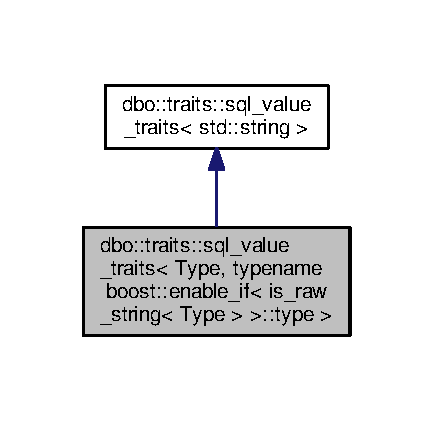
\includegraphics[width=208pt]{structdbo_1_1traits_1_1sql__value__traits_3_01_type_00_01typename_01boost_1_1enable__if_3_01is__5d4dab5346be40a7d7320f9b0590a003}
\end{center}
\end{figure}


Collaboration diagram for dbo\+:\+:traits\+:\+:sql\+\_\+value\+\_\+traits$<$ Type, typename boost\+:\+:enable\+\_\+if$<$ is\+\_\+raw\+\_\+string$<$ Type $>$ $>$\+:\+:type $>$\+:\nopagebreak
\begin{figure}[H]
\begin{center}
\leavevmode
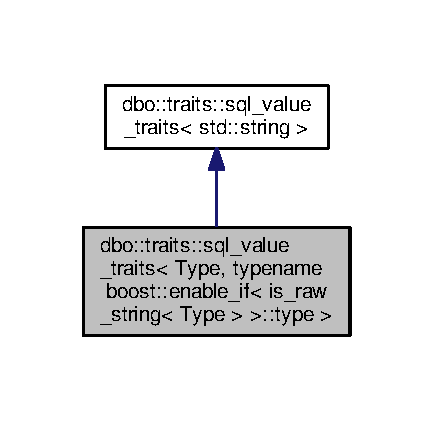
\includegraphics[width=208pt]{structdbo_1_1traits_1_1sql__value__traits_3_01_type_00_01typename_01boost_1_1enable__if_3_01is__09f9c416e24b79e8600cb3841ebf4f44}
\end{center}
\end{figure}
\subsection*{Static Public Member Functions}
\begin{DoxyCompactItemize}
\item 
static void \hyperlink{structdbo_1_1traits_1_1sql__value__traits_3_01_type_00_01typename_01boost_1_1enable__if_3_01is__aa5117fa5e949e5d70ea0660f0e85288_acc179a3184edb8ce906de3d47d7bc017}{bind} (const Type \&v, \hyperlink{classdbo_1_1stmt_1_1_statement}{stmt\+::\+Statement} \&statement, int size)
\end{DoxyCompactItemize}
\subsection*{Additional Inherited Members}


\subsection{Detailed Description}
\subsubsection*{template$<$typename Type$>$struct dbo\+::traits\+::sql\+\_\+value\+\_\+traits$<$ Type, typename boost\+::enable\+\_\+if$<$ is\+\_\+raw\+\_\+string$<$ Type $>$ $>$\+::type $>$}

This trait allow binding from literal string. Read is deactivated, you must use std\+::string to define table bindings 

\subsection{Member Function Documentation}
\hypertarget{structdbo_1_1traits_1_1sql__value__traits_3_01_type_00_01typename_01boost_1_1enable__if_3_01is__aa5117fa5e949e5d70ea0660f0e85288_acc179a3184edb8ce906de3d47d7bc017}{\index{dbo\+::traits\+::sql\+\_\+value\+\_\+traits$<$ Type, typename boost\+::enable\+\_\+if$<$ is\+\_\+raw\+\_\+string$<$ Type $>$ $>$\+::type $>$@{dbo\+::traits\+::sql\+\_\+value\+\_\+traits$<$ Type, typename boost\+::enable\+\_\+if$<$ is\+\_\+raw\+\_\+string$<$ Type $>$ $>$\+::type $>$}!bind@{bind}}
\index{bind@{bind}!dbo\+::traits\+::sql\+\_\+value\+\_\+traits$<$ Type, typename boost\+::enable\+\_\+if$<$ is\+\_\+raw\+\_\+string$<$ Type $>$ $>$\+::type $>$@{dbo\+::traits\+::sql\+\_\+value\+\_\+traits$<$ Type, typename boost\+::enable\+\_\+if$<$ is\+\_\+raw\+\_\+string$<$ Type $>$ $>$\+::type $>$}}
\subsubsection[{bind}]{\setlength{\rightskip}{0pt plus 5cm}template$<$typename Type $>$ static void {\bf dbo\+::traits\+::sql\+\_\+value\+\_\+traits}$<$ Type, typename boost\+::enable\+\_\+if$<$ {\bf is\+\_\+raw\+\_\+string}$<$ Type $>$ $>$\+::type $>$\+::bind (
\begin{DoxyParamCaption}
\item[{const Type \&}]{v, }
\item[{{\bf stmt\+::\+Statement} \&}]{statement, }
\item[{int}]{size}
\end{DoxyParamCaption}
)\hspace{0.3cm}{\ttfamily [inline]}, {\ttfamily [static]}}}\label{structdbo_1_1traits_1_1sql__value__traits_3_01_type_00_01typename_01boost_1_1enable__if_3_01is__aa5117fa5e949e5d70ea0660f0e85288_acc179a3184edb8ce906de3d47d7bc017}


The documentation for this struct was generated from the following file\+:\begin{DoxyCompactItemize}
\item 
dbo/traits/\hyperlink{_std_sql_traits_8h}{Std\+Sql\+Traits.\+h}\end{DoxyCompactItemize}

\hypertarget{classdbo_1_1traits_1_1_sql_postgres_types}{\section{dbo\+:\+:traits\+:\+:Sql\+Postgres\+Types Class Reference}
\label{classdbo_1_1traits_1_1_sql_postgres_types}\index{dbo\+::traits\+::\+Sql\+Postgres\+Types@{dbo\+::traits\+::\+Sql\+Postgres\+Types}}
}


{\ttfamily \#include $<$Sql\+Postgres\+Types.\+hpp$>$}

\subsection*{Public Types}
\begin{DoxyCompactItemize}
\item 
enum \hyperlink{classdbo_1_1traits_1_1_sql_postgres_types_ae4fe0e8ccef92e4330e470f407cabdea}{Sql\+Date\+Time\+Type} \{ \hyperlink{classdbo_1_1traits_1_1_sql_postgres_types_ae4fe0e8ccef92e4330e470f407cabdeaa522bb3ef71e99ebd0a0d7d806a5ac1d2}{Sql\+Date}, 
\hyperlink{classdbo_1_1traits_1_1_sql_postgres_types_ae4fe0e8ccef92e4330e470f407cabdeaac77f9a3f600090ebe2a9a3703340d5e5}{Sql\+Date\+Time}, 
\hyperlink{classdbo_1_1traits_1_1_sql_postgres_types_ae4fe0e8ccef92e4330e470f407cabdeaa9a7e92cc00af10d80e981f862e67964d}{Sql\+Time}
 \}
\begin{DoxyCompactList}\small\item\em Enum that defines a date time type. \end{DoxyCompactList}\end{DoxyCompactItemize}
\subsection*{Static Public Member Functions}
\begin{DoxyCompactItemize}
\item 
static std\+::string \hyperlink{classdbo_1_1traits_1_1_sql_postgres_types_a4126485ad2defdb510abc04b24ab20a9}{autoincrement\+Type} ()
\begin{DoxyCompactList}\small\item\em Returns the 'autoincrement' S\+Q\+L type. \end{DoxyCompactList}\item 
static std\+::string \hyperlink{classdbo_1_1traits_1_1_sql_postgres_types_a7a19608314c899a3455f650c98036e0b}{autoincrement\+Insert\+Suffix} (const std\+::string \&\hyperlink{namespacedbo_a8d25907296ae8360b3120b7492022c1d}{id})
\begin{DoxyCompactList}\small\item\em Returns the suffix for an 'autoincrement' insert statement. \end{DoxyCompactList}\item 
static std\+::string \hyperlink{classdbo_1_1traits_1_1_sql_postgres_types_a21d4da1f854986d3c941f1438c95a891}{date\+Time\+Type} (\hyperlink{classdbo_1_1traits_1_1_sql_postgres_types_ae4fe0e8ccef92e4330e470f407cabdea}{Sql\+Date\+Time\+Type} type)
\begin{DoxyCompactList}\small\item\em Returns the date/time type. \end{DoxyCompactList}\item 
static std\+::string \hyperlink{classdbo_1_1traits_1_1_sql_postgres_types_a787c62ab1b95709780c4196d541e210e}{blob\+Type} ()
\begin{DoxyCompactList}\small\item\em Returns the blob type. \end{DoxyCompactList}\item 
static std\+::string \hyperlink{classdbo_1_1traits_1_1_sql_postgres_types_abfa349db317aea7e888b6378301f9c6d}{text\+Type} (int size)
\begin{DoxyCompactList}\small\item\em Returns the text type. \end{DoxyCompactList}\item 
static std\+::string \hyperlink{classdbo_1_1traits_1_1_sql_postgres_types_a3a0bf17921987a36e44d0577cdad840d}{long\+Long\+Type} ()
\begin{DoxyCompactList}\small\item\em Returns the 64-\/bit integer type. \end{DoxyCompactList}\item 
static std\+::string \hyperlink{classdbo_1_1traits_1_1_sql_postgres_types_a4546fb422b2f00668453ea8eb7b4c17b}{boolean\+Type} ()
\begin{DoxyCompactList}\small\item\em Returns the boolean type. \end{DoxyCompactList}\end{DoxyCompactItemize}


\subsection{Member Enumeration Documentation}
\hypertarget{classdbo_1_1traits_1_1_sql_postgres_types_ae4fe0e8ccef92e4330e470f407cabdea}{\index{dbo\+::traits\+::\+Sql\+Postgres\+Types@{dbo\+::traits\+::\+Sql\+Postgres\+Types}!Sql\+Date\+Time\+Type@{Sql\+Date\+Time\+Type}}
\index{Sql\+Date\+Time\+Type@{Sql\+Date\+Time\+Type}!dbo\+::traits\+::\+Sql\+Postgres\+Types@{dbo\+::traits\+::\+Sql\+Postgres\+Types}}
\subsubsection[{Sql\+Date\+Time\+Type}]{\setlength{\rightskip}{0pt plus 5cm}enum {\bf dbo\+::traits\+::\+Sql\+Postgres\+Types\+::\+Sql\+Date\+Time\+Type}}}\label{classdbo_1_1traits_1_1_sql_postgres_types_ae4fe0e8ccef92e4330e470f407cabdea}


Enum that defines a date time type. 

\begin{Desc}
\item[Enumerator]\par
\begin{description}
\index{Sql\+Date@{Sql\+Date}!dbo\+::traits\+::\+Sql\+Postgres\+Types@{dbo\+::traits\+::\+Sql\+Postgres\+Types}}\index{dbo\+::traits\+::\+Sql\+Postgres\+Types@{dbo\+::traits\+::\+Sql\+Postgres\+Types}!Sql\+Date@{Sql\+Date}}\item[{\em 
\hypertarget{classdbo_1_1traits_1_1_sql_postgres_types_ae4fe0e8ccef92e4330e470f407cabdeaa522bb3ef71e99ebd0a0d7d806a5ac1d2}{Sql\+Date}\label{classdbo_1_1traits_1_1_sql_postgres_types_ae4fe0e8ccef92e4330e470f407cabdeaa522bb3ef71e99ebd0a0d7d806a5ac1d2}
}]Date only. \index{Sql\+Date\+Time@{Sql\+Date\+Time}!dbo\+::traits\+::\+Sql\+Postgres\+Types@{dbo\+::traits\+::\+Sql\+Postgres\+Types}}\index{dbo\+::traits\+::\+Sql\+Postgres\+Types@{dbo\+::traits\+::\+Sql\+Postgres\+Types}!Sql\+Date\+Time@{Sql\+Date\+Time}}\item[{\em 
\hypertarget{classdbo_1_1traits_1_1_sql_postgres_types_ae4fe0e8ccef92e4330e470f407cabdeaac77f9a3f600090ebe2a9a3703340d5e5}{Sql\+Date\+Time}\label{classdbo_1_1traits_1_1_sql_postgres_types_ae4fe0e8ccef92e4330e470f407cabdeaac77f9a3f600090ebe2a9a3703340d5e5}
}]Date and time. \index{Sql\+Time@{Sql\+Time}!dbo\+::traits\+::\+Sql\+Postgres\+Types@{dbo\+::traits\+::\+Sql\+Postgres\+Types}}\index{dbo\+::traits\+::\+Sql\+Postgres\+Types@{dbo\+::traits\+::\+Sql\+Postgres\+Types}!Sql\+Time@{Sql\+Time}}\item[{\em 
\hypertarget{classdbo_1_1traits_1_1_sql_postgres_types_ae4fe0e8ccef92e4330e470f407cabdeaa9a7e92cc00af10d80e981f862e67964d}{Sql\+Time}\label{classdbo_1_1traits_1_1_sql_postgres_types_ae4fe0e8ccef92e4330e470f407cabdeaa9a7e92cc00af10d80e981f862e67964d}
}]Time duration. \end{description}
\end{Desc}


\subsection{Member Function Documentation}
\hypertarget{classdbo_1_1traits_1_1_sql_postgres_types_a7a19608314c899a3455f650c98036e0b}{\index{dbo\+::traits\+::\+Sql\+Postgres\+Types@{dbo\+::traits\+::\+Sql\+Postgres\+Types}!autoincrement\+Insert\+Suffix@{autoincrement\+Insert\+Suffix}}
\index{autoincrement\+Insert\+Suffix@{autoincrement\+Insert\+Suffix}!dbo\+::traits\+::\+Sql\+Postgres\+Types@{dbo\+::traits\+::\+Sql\+Postgres\+Types}}
\subsubsection[{autoincrement\+Insert\+Suffix}]{\setlength{\rightskip}{0pt plus 5cm}static std\+::string dbo\+::traits\+::\+Sql\+Postgres\+Types\+::autoincrement\+Insert\+Suffix (
\begin{DoxyParamCaption}
\item[{const std\+::string \&}]{id}
\end{DoxyParamCaption}
)\hspace{0.3cm}{\ttfamily [inline]}, {\ttfamily [static]}}}\label{classdbo_1_1traits_1_1_sql_postgres_types_a7a19608314c899a3455f650c98036e0b}


Returns the suffix for an 'autoincrement' insert statement. 

This is appended to the {\ttfamily insert} statement, since some back-\/ends need to be indicated that they should return the autoincrement id. \hypertarget{classdbo_1_1traits_1_1_sql_postgres_types_a4126485ad2defdb510abc04b24ab20a9}{\index{dbo\+::traits\+::\+Sql\+Postgres\+Types@{dbo\+::traits\+::\+Sql\+Postgres\+Types}!autoincrement\+Type@{autoincrement\+Type}}
\index{autoincrement\+Type@{autoincrement\+Type}!dbo\+::traits\+::\+Sql\+Postgres\+Types@{dbo\+::traits\+::\+Sql\+Postgres\+Types}}
\subsubsection[{autoincrement\+Type}]{\setlength{\rightskip}{0pt plus 5cm}static std\+::string dbo\+::traits\+::\+Sql\+Postgres\+Types\+::autoincrement\+Type (
\begin{DoxyParamCaption}
{}
\end{DoxyParamCaption}
)\hspace{0.3cm}{\ttfamily [inline]}, {\ttfamily [static]}}}\label{classdbo_1_1traits_1_1_sql_postgres_types_a4126485ad2defdb510abc04b24ab20a9}


Returns the 'autoincrement' S\+Q\+L type. 

This is used by Session\+::create\+Tables() to create the {\itshape id} column. \hypertarget{classdbo_1_1traits_1_1_sql_postgres_types_a787c62ab1b95709780c4196d541e210e}{\index{dbo\+::traits\+::\+Sql\+Postgres\+Types@{dbo\+::traits\+::\+Sql\+Postgres\+Types}!blob\+Type@{blob\+Type}}
\index{blob\+Type@{blob\+Type}!dbo\+::traits\+::\+Sql\+Postgres\+Types@{dbo\+::traits\+::\+Sql\+Postgres\+Types}}
\subsubsection[{blob\+Type}]{\setlength{\rightskip}{0pt plus 5cm}static std\+::string dbo\+::traits\+::\+Sql\+Postgres\+Types\+::blob\+Type (
\begin{DoxyParamCaption}
{}
\end{DoxyParamCaption}
)\hspace{0.3cm}{\ttfamily [inline]}, {\ttfamily [static]}}}\label{classdbo_1_1traits_1_1_sql_postgres_types_a787c62ab1b95709780c4196d541e210e}


Returns the blob type. 

\begin{DoxySeeAlso}{See also}
Sql\+Statement\+::bind(int, const std\+::vector$<$unsigned char$>$\&) 
\end{DoxySeeAlso}
\hypertarget{classdbo_1_1traits_1_1_sql_postgres_types_a4546fb422b2f00668453ea8eb7b4c17b}{\index{dbo\+::traits\+::\+Sql\+Postgres\+Types@{dbo\+::traits\+::\+Sql\+Postgres\+Types}!boolean\+Type@{boolean\+Type}}
\index{boolean\+Type@{boolean\+Type}!dbo\+::traits\+::\+Sql\+Postgres\+Types@{dbo\+::traits\+::\+Sql\+Postgres\+Types}}
\subsubsection[{boolean\+Type}]{\setlength{\rightskip}{0pt plus 5cm}static std\+::string dbo\+::traits\+::\+Sql\+Postgres\+Types\+::boolean\+Type (
\begin{DoxyParamCaption}
{}
\end{DoxyParamCaption}
)\hspace{0.3cm}{\ttfamily [inline]}, {\ttfamily [static]}}}\label{classdbo_1_1traits_1_1_sql_postgres_types_a4546fb422b2f00668453ea8eb7b4c17b}


Returns the boolean type. 

This method will return \char`\"{}boolean\char`\"{} by default. \hypertarget{classdbo_1_1traits_1_1_sql_postgres_types_a21d4da1f854986d3c941f1438c95a891}{\index{dbo\+::traits\+::\+Sql\+Postgres\+Types@{dbo\+::traits\+::\+Sql\+Postgres\+Types}!date\+Time\+Type@{date\+Time\+Type}}
\index{date\+Time\+Type@{date\+Time\+Type}!dbo\+::traits\+::\+Sql\+Postgres\+Types@{dbo\+::traits\+::\+Sql\+Postgres\+Types}}
\subsubsection[{date\+Time\+Type}]{\setlength{\rightskip}{0pt plus 5cm}static std\+::string dbo\+::traits\+::\+Sql\+Postgres\+Types\+::date\+Time\+Type (
\begin{DoxyParamCaption}
\item[{{\bf Sql\+Date\+Time\+Type}}]{type}
\end{DoxyParamCaption}
)\hspace{0.3cm}{\ttfamily [inline]}, {\ttfamily [static]}}}\label{classdbo_1_1traits_1_1_sql_postgres_types_a21d4da1f854986d3c941f1438c95a891}


Returns the date/time type. 

\begin{DoxySeeAlso}{See also}
Sql\+Statement\+::bind(int, const boost\+::posix\+\_\+time\+::ptime\&, Sql\+Date\+Time\+Type) 
\end{DoxySeeAlso}
\hypertarget{classdbo_1_1traits_1_1_sql_postgres_types_a3a0bf17921987a36e44d0577cdad840d}{\index{dbo\+::traits\+::\+Sql\+Postgres\+Types@{dbo\+::traits\+::\+Sql\+Postgres\+Types}!long\+Long\+Type@{long\+Long\+Type}}
\index{long\+Long\+Type@{long\+Long\+Type}!dbo\+::traits\+::\+Sql\+Postgres\+Types@{dbo\+::traits\+::\+Sql\+Postgres\+Types}}
\subsubsection[{long\+Long\+Type}]{\setlength{\rightskip}{0pt plus 5cm}static std\+::string dbo\+::traits\+::\+Sql\+Postgres\+Types\+::long\+Long\+Type (
\begin{DoxyParamCaption}
{}
\end{DoxyParamCaption}
)\hspace{0.3cm}{\ttfamily [inline]}, {\ttfamily [static]}}}\label{classdbo_1_1traits_1_1_sql_postgres_types_a3a0bf17921987a36e44d0577cdad840d}


Returns the 64-\/bit integer type. 

This method will return \char`\"{}bigint\char`\"{} by default. \hypertarget{classdbo_1_1traits_1_1_sql_postgres_types_abfa349db317aea7e888b6378301f9c6d}{\index{dbo\+::traits\+::\+Sql\+Postgres\+Types@{dbo\+::traits\+::\+Sql\+Postgres\+Types}!text\+Type@{text\+Type}}
\index{text\+Type@{text\+Type}!dbo\+::traits\+::\+Sql\+Postgres\+Types@{dbo\+::traits\+::\+Sql\+Postgres\+Types}}
\subsubsection[{text\+Type}]{\setlength{\rightskip}{0pt plus 5cm}static std\+::string dbo\+::traits\+::\+Sql\+Postgres\+Types\+::text\+Type (
\begin{DoxyParamCaption}
\item[{int}]{size}
\end{DoxyParamCaption}
)\hspace{0.3cm}{\ttfamily [inline]}, {\ttfamily [static]}}}\label{classdbo_1_1traits_1_1_sql_postgres_types_abfa349db317aea7e888b6378301f9c6d}


Returns the text type. 

This is the text type for a string. If {\ttfamily size} = -\/1, then a type should be returned which does not require size information, otherwise a type should be returned that limits the size of the stored string to {\ttfamily size}.

This method will return \char`\"{}text\char`\"{} by default if size = -\/1, and \char`\"{}varchar(size)\char`\"{} otherwise.

\begin{DoxySeeAlso}{See also}
Sql\+Statement\+::bind(int column, const std\+::string\& value) 
\end{DoxySeeAlso}


The documentation for this class was generated from the following file\+:\begin{DoxyCompactItemize}
\item 
dbo/traits/\hyperlink{_sql_postgres_types_8hpp}{Sql\+Postgres\+Types.\+hpp}\end{DoxyCompactItemize}

\hypertarget{classdbo_1_1stmt_1_1_statement}{\section{dbo\+:\+:stmt\+:\+:Statement Class Reference}
\label{classdbo_1_1stmt_1_1_statement}\index{dbo\+::stmt\+::\+Statement@{dbo\+::stmt\+::\+Statement}}
}


{\ttfamily \#include $<$Statement.\+h$>$}



Inheritance diagram for dbo\+:\+:stmt\+:\+:Statement\+:\nopagebreak
\begin{figure}[H]
\begin{center}
\leavevmode
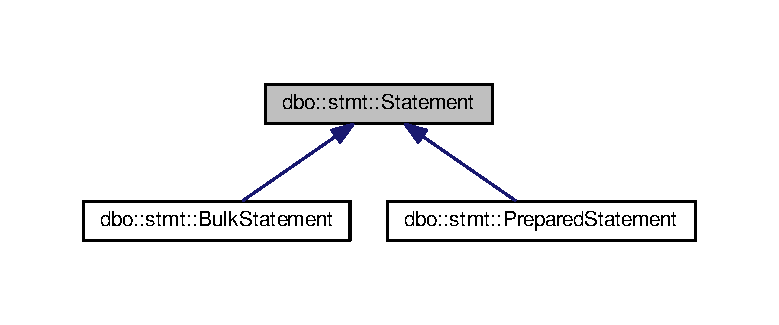
\includegraphics[width=350pt]{classdbo_1_1stmt_1_1_statement__inherit__graph}
\end{center}
\end{figure}


Collaboration diagram for dbo\+:\+:stmt\+:\+:Statement\+:\nopagebreak
\begin{figure}[H]
\begin{center}
\leavevmode
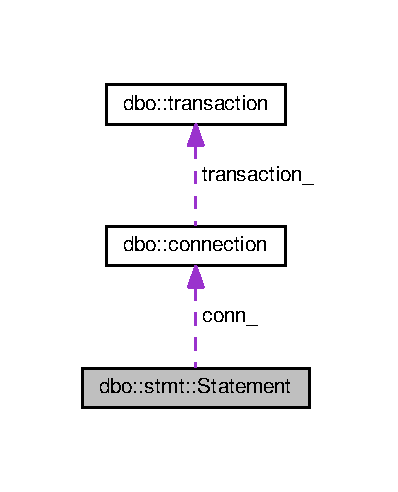
\includegraphics[width=191pt]{classdbo_1_1stmt_1_1_statement__coll__graph}
\end{center}
\end{figure}
\subsection*{Public Member Functions}
\begin{DoxyCompactItemize}
\item 
\hyperlink{classdbo_1_1stmt_1_1_statement_a6442da91d6cab533b92efdd2cb09bdff}{Statement} (\hyperlink{classdbo_1_1connection}{connection} \&conn)
\item 
virtual \hyperlink{classdbo_1_1stmt_1_1_statement_a57fdfef84b5f92d83850f6467b46012a}{$\sim$\+Statement} ()
\item 
virtual void \hyperlink{classdbo_1_1stmt_1_1_statement_a1699d7873785908a99211c91350cd376}{bind} ()=0
\item 
virtual void \hyperlink{classdbo_1_1stmt_1_1_statement_a8f2897467f5fccaec72ffe5ad797a8a3}{bind} (const std\+::string \&value)=0
\item 
virtual void \hyperlink{classdbo_1_1stmt_1_1_statement_a3f4f506b3df6f2d8667fa2900a662ee4}{bind} (const std\+::vector$<$ unsigned char $>$ \&value)=0
\item 
virtual bool \hyperlink{classdbo_1_1stmt_1_1_statement_a98ea71bb3c771dc5831b39d74035eb6b}{read} (char $\ast$\&value)=0
\item 
virtual bool \hyperlink{classdbo_1_1stmt_1_1_statement_a45864352cde548530425119915b3a2ef}{read} (std\+::vector$<$ unsigned char $>$ \&value)=0
\item 
virtual void \hyperlink{classdbo_1_1stmt_1_1_statement_af8e1a95b6c0c8b8ac6f5a25f4c48bf5e}{execute} ()=0
\end{DoxyCompactItemize}
\subsection*{Protected Attributes}
\begin{DoxyCompactItemize}
\item 
\hyperlink{classdbo_1_1connection}{connection} $\ast$ \hyperlink{classdbo_1_1stmt_1_1_statement_ae2fbf1f27c829b348afa751e7d04f934}{conn\+\_\+}
\end{DoxyCompactItemize}


\subsection{Constructor \& Destructor Documentation}
\hypertarget{classdbo_1_1stmt_1_1_statement_a6442da91d6cab533b92efdd2cb09bdff}{\index{dbo\+::stmt\+::\+Statement@{dbo\+::stmt\+::\+Statement}!Statement@{Statement}}
\index{Statement@{Statement}!dbo\+::stmt\+::\+Statement@{dbo\+::stmt\+::\+Statement}}
\subsubsection[{Statement}]{\setlength{\rightskip}{0pt plus 5cm}Statement\+::\+Statement (
\begin{DoxyParamCaption}
\item[{{\bf connection} \&}]{conn}
\end{DoxyParamCaption}
)}}\label{classdbo_1_1stmt_1_1_statement_a6442da91d6cab533b92efdd2cb09bdff}
Build a statement, the name of the statement will be created from the hash of the sql query \hypertarget{classdbo_1_1stmt_1_1_statement_a57fdfef84b5f92d83850f6467b46012a}{\index{dbo\+::stmt\+::\+Statement@{dbo\+::stmt\+::\+Statement}!````~Statement@{$\sim$\+Statement}}
\index{````~Statement@{$\sim$\+Statement}!dbo\+::stmt\+::\+Statement@{dbo\+::stmt\+::\+Statement}}
\subsubsection[{$\sim$\+Statement}]{\setlength{\rightskip}{0pt plus 5cm}Statement\+::$\sim$\+Statement (
\begin{DoxyParamCaption}
{}
\end{DoxyParamCaption}
)\hspace{0.3cm}{\ttfamily [virtual]}}}\label{classdbo_1_1stmt_1_1_statement_a57fdfef84b5f92d83850f6467b46012a}


\subsection{Member Function Documentation}
\hypertarget{classdbo_1_1stmt_1_1_statement_a1699d7873785908a99211c91350cd376}{\index{dbo\+::stmt\+::\+Statement@{dbo\+::stmt\+::\+Statement}!bind@{bind}}
\index{bind@{bind}!dbo\+::stmt\+::\+Statement@{dbo\+::stmt\+::\+Statement}}
\subsubsection[{bind}]{\setlength{\rightskip}{0pt plus 5cm}virtual void dbo\+::stmt\+::\+Statement\+::bind (
\begin{DoxyParamCaption}
{}
\end{DoxyParamCaption}
)\hspace{0.3cm}{\ttfamily [pure virtual]}}}\label{classdbo_1_1stmt_1_1_statement_a1699d7873785908a99211c91350cd376}
Bind a null value 

Implemented in \hyperlink{classdbo_1_1stmt_1_1_prepared_statement_a09a9cd82a4d0123b679312acf74fbd02}{dbo\+::stmt\+::\+Prepared\+Statement}, and \hyperlink{classdbo_1_1stmt_1_1_bulk_statement_ae40b794caf52eb3e1cafaef7eeb2042c}{dbo\+::stmt\+::\+Bulk\+Statement}.

\hypertarget{classdbo_1_1stmt_1_1_statement_a8f2897467f5fccaec72ffe5ad797a8a3}{\index{dbo\+::stmt\+::\+Statement@{dbo\+::stmt\+::\+Statement}!bind@{bind}}
\index{bind@{bind}!dbo\+::stmt\+::\+Statement@{dbo\+::stmt\+::\+Statement}}
\subsubsection[{bind}]{\setlength{\rightskip}{0pt plus 5cm}virtual void dbo\+::stmt\+::\+Statement\+::bind (
\begin{DoxyParamCaption}
\item[{const std\+::string \&}]{value}
\end{DoxyParamCaption}
)\hspace{0.3cm}{\ttfamily [pure virtual]}}}\label{classdbo_1_1stmt_1_1_statement_a8f2897467f5fccaec72ffe5ad797a8a3}
Bind a string value 

Implemented in \hyperlink{classdbo_1_1stmt_1_1_prepared_statement_a50a8195e7156004c2bf8533a89eb4541}{dbo\+::stmt\+::\+Prepared\+Statement}, and \hyperlink{classdbo_1_1stmt_1_1_bulk_statement_ae12881728ef31a7acc0903d7473a8cb9}{dbo\+::stmt\+::\+Bulk\+Statement}.

\hypertarget{classdbo_1_1stmt_1_1_statement_a3f4f506b3df6f2d8667fa2900a662ee4}{\index{dbo\+::stmt\+::\+Statement@{dbo\+::stmt\+::\+Statement}!bind@{bind}}
\index{bind@{bind}!dbo\+::stmt\+::\+Statement@{dbo\+::stmt\+::\+Statement}}
\subsubsection[{bind}]{\setlength{\rightskip}{0pt plus 5cm}virtual void dbo\+::stmt\+::\+Statement\+::bind (
\begin{DoxyParamCaption}
\item[{const std\+::vector$<$ unsigned char $>$ \&}]{value}
\end{DoxyParamCaption}
)\hspace{0.3cm}{\ttfamily [pure virtual]}}}\label{classdbo_1_1stmt_1_1_statement_a3f4f506b3df6f2d8667fa2900a662ee4}
Bind a binary value 

Implemented in \hyperlink{classdbo_1_1stmt_1_1_prepared_statement_ac569d72f107737acda7ce94c831f5838}{dbo\+::stmt\+::\+Prepared\+Statement}, and \hyperlink{classdbo_1_1stmt_1_1_bulk_statement_a36ca4fb16d32d17b838fe4604ebf2139}{dbo\+::stmt\+::\+Bulk\+Statement}.

\hypertarget{classdbo_1_1stmt_1_1_statement_af8e1a95b6c0c8b8ac6f5a25f4c48bf5e}{\index{dbo\+::stmt\+::\+Statement@{dbo\+::stmt\+::\+Statement}!execute@{execute}}
\index{execute@{execute}!dbo\+::stmt\+::\+Statement@{dbo\+::stmt\+::\+Statement}}
\subsubsection[{execute}]{\setlength{\rightskip}{0pt plus 5cm}virtual void dbo\+::stmt\+::\+Statement\+::execute (
\begin{DoxyParamCaption}
{}
\end{DoxyParamCaption}
)\hspace{0.3cm}{\ttfamily [pure virtual]}}}\label{classdbo_1_1stmt_1_1_statement_af8e1a95b6c0c8b8ac6f5a25f4c48bf5e}
Execute the prepared statement 

Implemented in \hyperlink{classdbo_1_1stmt_1_1_prepared_statement_a1f14d39e3ce01f550527b606ec7e16ab}{dbo\+::stmt\+::\+Prepared\+Statement}, and \hyperlink{classdbo_1_1stmt_1_1_bulk_statement_af2cde35cc87094525b4dc1e4dc99c710}{dbo\+::stmt\+::\+Bulk\+Statement}.

\hypertarget{classdbo_1_1stmt_1_1_statement_a98ea71bb3c771dc5831b39d74035eb6b}{\index{dbo\+::stmt\+::\+Statement@{dbo\+::stmt\+::\+Statement}!read@{read}}
\index{read@{read}!dbo\+::stmt\+::\+Statement@{dbo\+::stmt\+::\+Statement}}
\subsubsection[{read}]{\setlength{\rightskip}{0pt plus 5cm}virtual bool dbo\+::stmt\+::\+Statement\+::read (
\begin{DoxyParamCaption}
\item[{char $\ast$\&}]{value}
\end{DoxyParamCaption}
)\hspace{0.3cm}{\ttfamily [pure virtual]}}}\label{classdbo_1_1stmt_1_1_statement_a98ea71bb3c771dc5831b39d74035eb6b}
Read content to string 

Implemented in \hyperlink{classdbo_1_1stmt_1_1_prepared_statement_ab01ebe611bfdb2a17cc10e7edbb29d4f}{dbo\+::stmt\+::\+Prepared\+Statement}, and \hyperlink{classdbo_1_1stmt_1_1_bulk_statement_ae789fa6e80389758303064fcceafb597}{dbo\+::stmt\+::\+Bulk\+Statement}.

\hypertarget{classdbo_1_1stmt_1_1_statement_a45864352cde548530425119915b3a2ef}{\index{dbo\+::stmt\+::\+Statement@{dbo\+::stmt\+::\+Statement}!read@{read}}
\index{read@{read}!dbo\+::stmt\+::\+Statement@{dbo\+::stmt\+::\+Statement}}
\subsubsection[{read}]{\setlength{\rightskip}{0pt plus 5cm}virtual bool dbo\+::stmt\+::\+Statement\+::read (
\begin{DoxyParamCaption}
\item[{std\+::vector$<$ unsigned char $>$ \&}]{value}
\end{DoxyParamCaption}
)\hspace{0.3cm}{\ttfamily [pure virtual]}}}\label{classdbo_1_1stmt_1_1_statement_a45864352cde548530425119915b3a2ef}
Read content to binary array 

Implemented in \hyperlink{classdbo_1_1stmt_1_1_prepared_statement_a65620d8b28b279d717ed6a787f89ad70}{dbo\+::stmt\+::\+Prepared\+Statement}, and \hyperlink{classdbo_1_1stmt_1_1_bulk_statement_aaa5722c838af4203ae19bd94448d63dd}{dbo\+::stmt\+::\+Bulk\+Statement}.



\subsection{Member Data Documentation}
\hypertarget{classdbo_1_1stmt_1_1_statement_ae2fbf1f27c829b348afa751e7d04f934}{\index{dbo\+::stmt\+::\+Statement@{dbo\+::stmt\+::\+Statement}!conn\+\_\+@{conn\+\_\+}}
\index{conn\+\_\+@{conn\+\_\+}!dbo\+::stmt\+::\+Statement@{dbo\+::stmt\+::\+Statement}}
\subsubsection[{conn\+\_\+}]{\setlength{\rightskip}{0pt plus 5cm}{\bf connection}$\ast$ dbo\+::stmt\+::\+Statement\+::conn\+\_\+\hspace{0.3cm}{\ttfamily [protected]}}}\label{classdbo_1_1stmt_1_1_statement_ae2fbf1f27c829b348afa751e7d04f934}


The documentation for this class was generated from the following files\+:\begin{DoxyCompactItemize}
\item 
dbo/stmt/\hyperlink{_statement_8h}{Statement.\+h}\item 
dbo/stmt/\hyperlink{_statement_8cpp}{Statement.\+cpp}\end{DoxyCompactItemize}

\hypertarget{classdbo_1_1transaction}{\section{dbo\+:\+:transaction Class Reference}
\label{classdbo_1_1transaction}\index{dbo\+::transaction@{dbo\+::transaction}}
}


{\ttfamily \#include $<$transaction.\+h$>$}

\subsection*{Public Member Functions}
\begin{DoxyCompactItemize}
\item 
\hyperlink{classdbo_1_1transaction_a9230c3550e5bbbbaf01af153caa7b8ee}{$\sim$transaction} () noexcept(false)
\begin{DoxyCompactList}\small\item\em Destructor. \end{DoxyCompactList}\item 
bool \hyperlink{classdbo_1_1transaction_ad3586b191113f790957095f1fdc1bd74}{active} () const 
\begin{DoxyCompactList}\small\item\em Returns whether the transaction is still active. \end{DoxyCompactList}\item 
void \hyperlink{classdbo_1_1transaction_a4cd2f57757397b26e69cefda212fd292}{commit} ()
\begin{DoxyCompactList}\small\item\em Commits the transaction. \end{DoxyCompactList}\item 
void \hyperlink{classdbo_1_1transaction_a0cc9d5fb8dcfd391e64c5477119afab4}{rollback} ()
\begin{DoxyCompactList}\small\item\em Rolls back the transaction. \end{DoxyCompactList}\end{DoxyCompactItemize}
\subsection*{Protected Member Functions}
\begin{DoxyCompactItemize}
\item 
\hyperlink{classdbo_1_1transaction_a91895b970904b28405ab3e2d6c7671af}{transaction} (\hyperlink{classdbo_1_1connection}{connection} \&conn)
\begin{DoxyCompactList}\small\item\em Constructor. \end{DoxyCompactList}\item 
void \hyperlink{classdbo_1_1transaction_a6f14176b1b69158df1bf0dca9cae20d2}{open} ()
\end{DoxyCompactItemize}


\subsection{Constructor \& Destructor Documentation}
\hypertarget{classdbo_1_1transaction_a9230c3550e5bbbbaf01af153caa7b8ee}{\index{dbo\+::transaction@{dbo\+::transaction}!````~transaction@{$\sim$transaction}}
\index{````~transaction@{$\sim$transaction}!dbo\+::transaction@{dbo\+::transaction}}
\subsubsection[{$\sim$transaction}]{\setlength{\rightskip}{0pt plus 5cm}transaction\+::$\sim$transaction (
\begin{DoxyParamCaption}
{}
\end{DoxyParamCaption}
)\hspace{0.3cm}{\ttfamily [noexcept]}}}\label{classdbo_1_1transaction_a9230c3550e5bbbbaf01af153caa7b8ee}


Destructor. 

If the transaction is still active, it is rolled back. \hypertarget{classdbo_1_1transaction_a91895b970904b28405ab3e2d6c7671af}{\index{dbo\+::transaction@{dbo\+::transaction}!transaction@{transaction}}
\index{transaction@{transaction}!dbo\+::transaction@{dbo\+::transaction}}
\subsubsection[{transaction}]{\setlength{\rightskip}{0pt plus 5cm}transaction\+::transaction (
\begin{DoxyParamCaption}
\item[{{\bf connection} \&}]{conn}
\end{DoxyParamCaption}
)\hspace{0.3cm}{\ttfamily [protected]}}}\label{classdbo_1_1transaction_a91895b970904b28405ab3e2d6c7671af}


Constructor. 

Opens a transaction for the given {\ttfamily session}. If a transaction is already open for the connection nothing is done. 

\subsection{Member Function Documentation}
\hypertarget{classdbo_1_1transaction_ad3586b191113f790957095f1fdc1bd74}{\index{dbo\+::transaction@{dbo\+::transaction}!active@{active}}
\index{active@{active}!dbo\+::transaction@{dbo\+::transaction}}
\subsubsection[{active}]{\setlength{\rightskip}{0pt plus 5cm}bool transaction\+::active (
\begin{DoxyParamCaption}
{}
\end{DoxyParamCaption}
) const}}\label{classdbo_1_1transaction_ad3586b191113f790957095f1fdc1bd74}


Returns whether the transaction is still active. 

A transaction is active unless it has been committed or rolled back.

While a transaction is active, new transactions for the same session are treated as the same transaction. Nested transactions are not implemented. \hypertarget{classdbo_1_1transaction_a4cd2f57757397b26e69cefda212fd292}{\index{dbo\+::transaction@{dbo\+::transaction}!commit@{commit}}
\index{commit@{commit}!dbo\+::transaction@{dbo\+::transaction}}
\subsubsection[{commit}]{\setlength{\rightskip}{0pt plus 5cm}void transaction\+::commit (
\begin{DoxyParamCaption}
{}
\end{DoxyParamCaption}
)}}\label{classdbo_1_1transaction_a4cd2f57757397b26e69cefda212fd292}


Commits the transaction. 

\begin{DoxySeeAlso}{See also}
\hyperlink{classdbo_1_1transaction_a0cc9d5fb8dcfd391e64c5477119afab4}{rollback()} 
\end{DoxySeeAlso}
\hypertarget{classdbo_1_1transaction_a6f14176b1b69158df1bf0dca9cae20d2}{\index{dbo\+::transaction@{dbo\+::transaction}!open@{open}}
\index{open@{open}!dbo\+::transaction@{dbo\+::transaction}}
\subsubsection[{open}]{\setlength{\rightskip}{0pt plus 5cm}void transaction\+::open (
\begin{DoxyParamCaption}
{}
\end{DoxyParamCaption}
)\hspace{0.3cm}{\ttfamily [protected]}}}\label{classdbo_1_1transaction_a6f14176b1b69158df1bf0dca9cae20d2}
\hypertarget{classdbo_1_1transaction_a0cc9d5fb8dcfd391e64c5477119afab4}{\index{dbo\+::transaction@{dbo\+::transaction}!rollback@{rollback}}
\index{rollback@{rollback}!dbo\+::transaction@{dbo\+::transaction}}
\subsubsection[{rollback}]{\setlength{\rightskip}{0pt plus 5cm}void transaction\+::rollback (
\begin{DoxyParamCaption}
{}
\end{DoxyParamCaption}
)}}\label{classdbo_1_1transaction_a0cc9d5fb8dcfd391e64c5477119afab4}


Rolls back the transaction. 

\begin{DoxySeeAlso}{See also}
\hyperlink{classdbo_1_1transaction_a4cd2f57757397b26e69cefda212fd292}{commit()} 
\end{DoxySeeAlso}


The documentation for this class was generated from the following files\+:\begin{DoxyCompactItemize}
\item 
dbo/\hyperlink{transaction_8h}{transaction.\+h}\item 
dbo/\hyperlink{transaction_8cpp}{transaction.\+cpp}\end{DoxyCompactItemize}

\hypertarget{structdbo_1_1connection_1_1typecomp}{\section{dbo\+:\+:connection\+:\+:typecomp Struct Reference}
\label{structdbo_1_1connection_1_1typecomp}\index{dbo\+::connection\+::typecomp@{dbo\+::connection\+::typecomp}}
}


{\ttfamily \#include $<$connection.\+h$>$}

\subsection*{Public Member Functions}
\begin{DoxyCompactItemize}
\item 
bool \hyperlink{structdbo_1_1connection_1_1typecomp_ab495e5661ce6917a54bb79e108cc0a55}{operator()} (const \hyperlink{classdbo_1_1connection_ad9b28dcf5699796d552af8a159f03a5a}{const\+\_\+typeinfo\+\_\+ptr} \&lhs, const \hyperlink{classdbo_1_1connection_ad9b28dcf5699796d552af8a159f03a5a}{const\+\_\+typeinfo\+\_\+ptr} \&rhs) const 
\end{DoxyCompactItemize}


\subsection{Member Function Documentation}
\hypertarget{structdbo_1_1connection_1_1typecomp_ab495e5661ce6917a54bb79e108cc0a55}{\index{dbo\+::connection\+::typecomp@{dbo\+::connection\+::typecomp}!operator()@{operator()}}
\index{operator()@{operator()}!dbo\+::connection\+::typecomp@{dbo\+::connection\+::typecomp}}
\subsubsection[{operator()}]{\setlength{\rightskip}{0pt plus 5cm}bool dbo\+::connection\+::typecomp\+::operator() (
\begin{DoxyParamCaption}
\item[{const {\bf const\+\_\+typeinfo\+\_\+ptr} \&}]{lhs, }
\item[{const {\bf const\+\_\+typeinfo\+\_\+ptr} \&}]{rhs}
\end{DoxyParamCaption}
) const\hspace{0.3cm}{\ttfamily [inline]}}}\label{structdbo_1_1connection_1_1typecomp_ab495e5661ce6917a54bb79e108cc0a55}


The documentation for this struct was generated from the following file\+:\begin{DoxyCompactItemize}
\item 
dbo/\hyperlink{connection_8h}{connection.\+h}\end{DoxyCompactItemize}

\hypertarget{classdbo_1_1action_1_1_update}{\section{dbo\+:\+:action\+:\+:Update$<$ C $>$ Class Template Reference}
\label{classdbo_1_1action_1_1_update}\index{dbo\+::action\+::\+Update$<$ C $>$@{dbo\+::action\+::\+Update$<$ C $>$}}
}


{\ttfamily \#include $<$Update.\+hpp$>$}

\subsection*{Public Types}
\begin{DoxyCompactItemize}
\item 
using \hyperlink{classdbo_1_1action_1_1_update_ade7e784c4031bf879160b8934ef4414b}{Id\+Type} = typename \hyperlink{structdbo_1_1traits_1_1dbo__traits}{traits\+::dbo\+\_\+traits}$<$ C $>$\+::\hyperlink{classdbo_1_1action_1_1_update_ade7e784c4031bf879160b8934ef4414b}{Id\+Type}
\end{DoxyCompactItemize}
\subsection*{Public Member Functions}
\begin{DoxyCompactItemize}
\item 
\hyperlink{classdbo_1_1action_1_1_update_aab7708faf49011e9f40b07ed389abc8e}{Update} (\hyperlink{classdbo_1_1ptr}{ptr}$<$ C $>$ \hyperlink{classdbo_1_1ptr}{ptr}, std\+::shared\+\_\+ptr$<$ \hyperlink{classdbo_1_1mapping_1_1_mapping}{mapping\+::\+Mapping}$<$ C $>$$>$ mapping, \hyperlink{classdbo_1_1stmt_1_1_prepared_statement}{stmt\+::\+Prepared\+Statement} \&stmt)
\item 
void \hyperlink{classdbo_1_1action_1_1_update_aafb60921a5d7d4508b9356637e7aeaa1}{visit} ()
\item 
{\footnotesize template$<$typename V $>$ }\\void \hyperlink{classdbo_1_1action_1_1_update_a1c18a9ecafe6f92586e60c4c6c10e05d}{act} (const \hyperlink{classdbo_1_1mapping_1_1_field_ref}{mapping\+::\+Field\+Ref}$<$ V $>$ \&\hyperlink{namespacedbo_ad1f50f02cb050acf946807959252a93f}{field})
\item 
{\footnotesize template$<$typename V $>$ }\\void \hyperlink{classdbo_1_1action_1_1_update_a86d4d6a33f11bbf22dc4bea748c1e555}{act\+Id} (V \&value, const std\+::string \&name, int size)
\item 
{\footnotesize template$<$class D $>$ }\\void \hyperlink{classdbo_1_1action_1_1_update_aa86b704191e37df75e8c7927c5ded490}{act\+Id} (\hyperlink{classdbo_1_1ptr}{ptr}$<$ D $>$ \&value, const std\+::string \&name, int size, int fk\+Constraints)
\item 
{\footnotesize template$<$class D $>$ }\\void \hyperlink{classdbo_1_1action_1_1_update_a045d466453a9411faa348b071af0ccdf}{act\+Ptr} (const \hyperlink{classdbo_1_1mapping_1_1_ptr_ref}{mapping\+::\+Ptr\+Ref}$<$ D $>$ \&\hyperlink{namespacedbo_ad1f50f02cb050acf946807959252a93f}{field})
\item 
\hyperlink{classdbo_1_1connection}{connection} \& \hyperlink{classdbo_1_1action_1_1_update_a8983e7608f961b79732b6b60a140afd5}{conn} ()
\end{DoxyCompactItemize}
\subsection*{Friends}
\begin{DoxyCompactItemize}
\item 
{\footnotesize template$<$class D $>$ }\\class \hyperlink{classdbo_1_1action_1_1_update_a440e8361659c899ef7f0651ec5ea49e8}{Update}
\end{DoxyCompactItemize}


\subsection{Member Typedef Documentation}
\hypertarget{classdbo_1_1action_1_1_update_ade7e784c4031bf879160b8934ef4414b}{\index{dbo\+::action\+::\+Update@{dbo\+::action\+::\+Update}!Id\+Type@{Id\+Type}}
\index{Id\+Type@{Id\+Type}!dbo\+::action\+::\+Update@{dbo\+::action\+::\+Update}}
\subsubsection[{Id\+Type}]{\setlength{\rightskip}{0pt plus 5cm}template$<$class C $>$ using {\bf dbo\+::action\+::\+Update}$<$ C $>$\+::{\bf Id\+Type} =  typename {\bf traits\+::dbo\+\_\+traits}$<$C$>$\+::{\bf Id\+Type}}}\label{classdbo_1_1action_1_1_update_ade7e784c4031bf879160b8934ef4414b}


\subsection{Constructor \& Destructor Documentation}
\hypertarget{classdbo_1_1action_1_1_update_aab7708faf49011e9f40b07ed389abc8e}{\index{dbo\+::action\+::\+Update@{dbo\+::action\+::\+Update}!Update@{Update}}
\index{Update@{Update}!dbo\+::action\+::\+Update@{dbo\+::action\+::\+Update}}
\subsubsection[{Update}]{\setlength{\rightskip}{0pt plus 5cm}template$<$class C $>$ {\bf dbo\+::action\+::\+Update}$<$ C $>$\+::{\bf Update} (
\begin{DoxyParamCaption}
\item[{{\bf ptr}$<$ C $>$}]{ptr, }
\item[{std\+::shared\+\_\+ptr$<$ {\bf mapping\+::\+Mapping}$<$ C $>$$>$}]{mapping, }
\item[{{\bf stmt\+::\+Prepared\+Statement} \&}]{stmt}
\end{DoxyParamCaption}
)}}\label{classdbo_1_1action_1_1_update_aab7708faf49011e9f40b07ed389abc8e}


\subsection{Member Function Documentation}
\hypertarget{classdbo_1_1action_1_1_update_a1c18a9ecafe6f92586e60c4c6c10e05d}{\index{dbo\+::action\+::\+Update@{dbo\+::action\+::\+Update}!act@{act}}
\index{act@{act}!dbo\+::action\+::\+Update@{dbo\+::action\+::\+Update}}
\subsubsection[{act}]{\setlength{\rightskip}{0pt plus 5cm}template$<$class C $>$ template$<$typename V $>$ void {\bf dbo\+::action\+::\+Update}$<$ C $>$\+::act (
\begin{DoxyParamCaption}
\item[{const {\bf mapping\+::\+Field\+Ref}$<$ V $>$ \&}]{field}
\end{DoxyParamCaption}
)}}\label{classdbo_1_1action_1_1_update_a1c18a9ecafe6f92586e60c4c6c10e05d}
\hypertarget{classdbo_1_1action_1_1_update_a86d4d6a33f11bbf22dc4bea748c1e555}{\index{dbo\+::action\+::\+Update@{dbo\+::action\+::\+Update}!act\+Id@{act\+Id}}
\index{act\+Id@{act\+Id}!dbo\+::action\+::\+Update@{dbo\+::action\+::\+Update}}
\subsubsection[{act\+Id}]{\setlength{\rightskip}{0pt plus 5cm}template$<$class C $>$ template$<$typename V $>$ void {\bf dbo\+::action\+::\+Update}$<$ C $>$\+::act\+Id (
\begin{DoxyParamCaption}
\item[{V \&}]{value, }
\item[{const std\+::string \&}]{name, }
\item[{int}]{size}
\end{DoxyParamCaption}
)}}\label{classdbo_1_1action_1_1_update_a86d4d6a33f11bbf22dc4bea748c1e555}
\hypertarget{classdbo_1_1action_1_1_update_aa86b704191e37df75e8c7927c5ded490}{\index{dbo\+::action\+::\+Update@{dbo\+::action\+::\+Update}!act\+Id@{act\+Id}}
\index{act\+Id@{act\+Id}!dbo\+::action\+::\+Update@{dbo\+::action\+::\+Update}}
\subsubsection[{act\+Id}]{\setlength{\rightskip}{0pt plus 5cm}template$<$class C $>$ template$<$class D $>$ void {\bf dbo\+::action\+::\+Update}$<$ C $>$\+::act\+Id (
\begin{DoxyParamCaption}
\item[{{\bf ptr}$<$ D $>$ \&}]{value, }
\item[{const std\+::string \&}]{name, }
\item[{int}]{size, }
\item[{int}]{fk\+Constraints}
\end{DoxyParamCaption}
)}}\label{classdbo_1_1action_1_1_update_aa86b704191e37df75e8c7927c5ded490}
\hypertarget{classdbo_1_1action_1_1_update_a045d466453a9411faa348b071af0ccdf}{\index{dbo\+::action\+::\+Update@{dbo\+::action\+::\+Update}!act\+Ptr@{act\+Ptr}}
\index{act\+Ptr@{act\+Ptr}!dbo\+::action\+::\+Update@{dbo\+::action\+::\+Update}}
\subsubsection[{act\+Ptr}]{\setlength{\rightskip}{0pt plus 5cm}template$<$class C $>$ template$<$class D $>$ void {\bf dbo\+::action\+::\+Update}$<$ C $>$\+::act\+Ptr (
\begin{DoxyParamCaption}
\item[{const {\bf mapping\+::\+Ptr\+Ref}$<$ D $>$ \&}]{field}
\end{DoxyParamCaption}
)}}\label{classdbo_1_1action_1_1_update_a045d466453a9411faa348b071af0ccdf}
\hypertarget{classdbo_1_1action_1_1_update_a8983e7608f961b79732b6b60a140afd5}{\index{dbo\+::action\+::\+Update@{dbo\+::action\+::\+Update}!conn@{conn}}
\index{conn@{conn}!dbo\+::action\+::\+Update@{dbo\+::action\+::\+Update}}
\subsubsection[{conn}]{\setlength{\rightskip}{0pt plus 5cm}template$<$class C $>$ {\bf connection}\& {\bf dbo\+::action\+::\+Update}$<$ C $>$\+::conn (
\begin{DoxyParamCaption}
{}
\end{DoxyParamCaption}
)\hspace{0.3cm}{\ttfamily [inline]}}}\label{classdbo_1_1action_1_1_update_a8983e7608f961b79732b6b60a140afd5}
\hypertarget{classdbo_1_1action_1_1_update_aafb60921a5d7d4508b9356637e7aeaa1}{\index{dbo\+::action\+::\+Update@{dbo\+::action\+::\+Update}!visit@{visit}}
\index{visit@{visit}!dbo\+::action\+::\+Update@{dbo\+::action\+::\+Update}}
\subsubsection[{visit}]{\setlength{\rightskip}{0pt plus 5cm}template$<$class C $>$ void {\bf dbo\+::action\+::\+Update}$<$ C $>$\+::visit (
\begin{DoxyParamCaption}
{}
\end{DoxyParamCaption}
)}}\label{classdbo_1_1action_1_1_update_aafb60921a5d7d4508b9356637e7aeaa1}


\subsection{Friends And Related Function Documentation}
\hypertarget{classdbo_1_1action_1_1_update_a440e8361659c899ef7f0651ec5ea49e8}{\index{dbo\+::action\+::\+Update@{dbo\+::action\+::\+Update}!Update@{Update}}
\index{Update@{Update}!dbo\+::action\+::\+Update@{dbo\+::action\+::\+Update}}
\subsubsection[{Update}]{\setlength{\rightskip}{0pt plus 5cm}template$<$class C $>$ template$<$class D $>$ friend class {\bf Update}\hspace{0.3cm}{\ttfamily [friend]}}}\label{classdbo_1_1action_1_1_update_a440e8361659c899ef7f0651ec5ea49e8}


The documentation for this class was generated from the following files\+:\begin{DoxyCompactItemize}
\item 
dbo/action/\hyperlink{_update_8hpp}{Update.\+hpp}\item 
dbo/action/\hyperlink{_update_8cxx}{Update.\+cxx}\end{DoxyCompactItemize}

\chapter{File Documentation}
\hypertarget{_action_option_8cpp}{\section{dbo/action/\+Action\+Option.cpp File Reference}
\label{_action_option_8cpp}\index{dbo/action/\+Action\+Option.\+cpp@{dbo/action/\+Action\+Option.\+cpp}}
}
{\ttfamily \#include \char`\"{}dbo/action/\+Action\+Option.\+h\char`\"{}}\\*
Include dependency graph for Action\+Option.\+cpp\+:\nopagebreak
\begin{figure}[H]
\begin{center}
\leavevmode
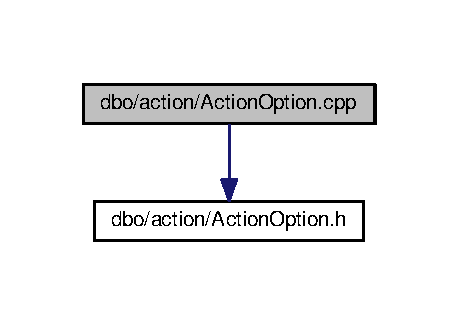
\includegraphics[width=220pt]{_action_option_8cpp__incl}
\end{center}
\end{figure}
\subsection*{Functions}
\begin{DoxyCompactItemize}
\item 
\hyperlink{classdbo_1_1_action_option}{Action\+Option} \hyperlink{_action_option_8cpp_a252c993cf11e1a6c6d45e6443ce0e603}{operator$\vert$} (\hyperlink{classdbo_1_1_action_option}{Action\+Option} lhs, \hyperlink{classdbo_1_1_action_option}{Action\+Option} rhs)
\begin{DoxyCompactList}\small\item\em Combines two options. \end{DoxyCompactList}\end{DoxyCompactItemize}


\subsection{Function Documentation}
\hypertarget{_action_option_8cpp_a252c993cf11e1a6c6d45e6443ce0e603}{\index{Action\+Option.\+cpp@{Action\+Option.\+cpp}!operator\texttt{"|}@{operator\texttt{"|}}}
\index{operator\texttt{"|}@{operator\texttt{"|}}!Action\+Option.\+cpp@{Action\+Option.\+cpp}}
\subsubsection[{operator\texttt{"|}}]{\setlength{\rightskip}{0pt plus 5cm}{\bf Action\+Option} operator$\vert$ (
\begin{DoxyParamCaption}
\item[{{\bf Action\+Option}}]{lhs, }
\item[{{\bf Action\+Option}}]{rhs}
\end{DoxyParamCaption}
)}}\label{_action_option_8cpp_a252c993cf11e1a6c6d45e6443ce0e603}


Combines two options. 


\hypertarget{_action_option_8h}{\section{dbo/action/\+Action\+Option.h File Reference}
\label{_action_option_8h}\index{dbo/action/\+Action\+Option.\+h@{dbo/action/\+Action\+Option.\+h}}
}
This graph shows which files directly or indirectly include this file\+:\nopagebreak
\begin{figure}[H]
\begin{center}
\leavevmode
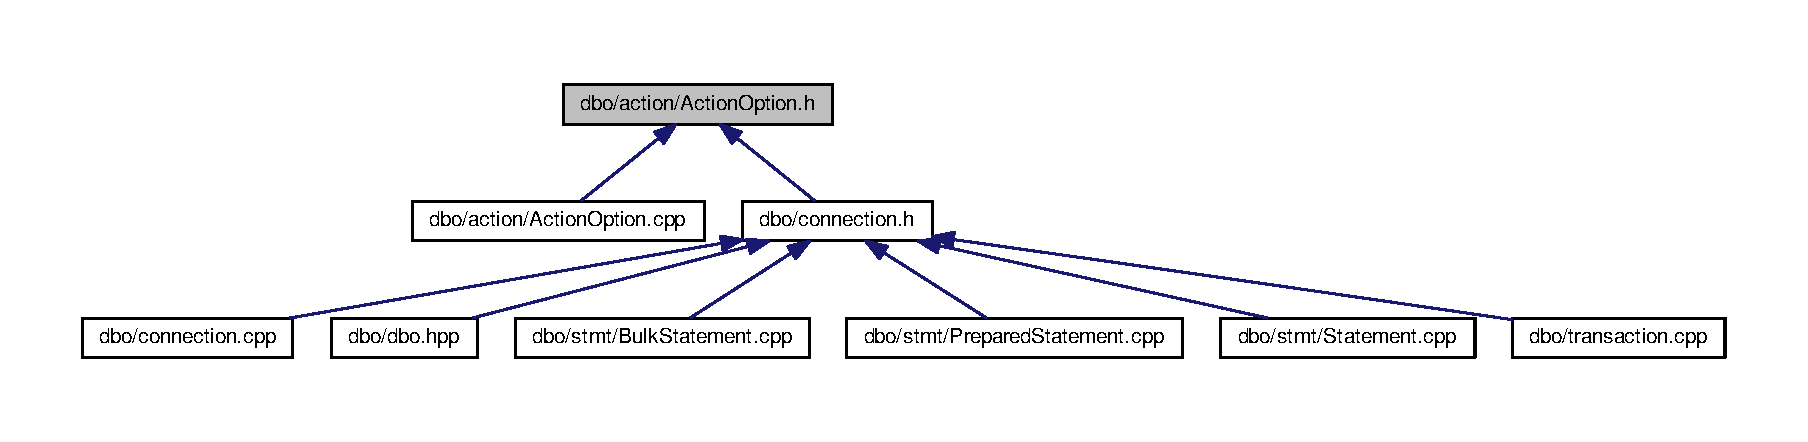
\includegraphics[width=350pt]{_action_option_8h__dep__incl}
\end{center}
\end{figure}
\subsection*{Classes}
\begin{DoxyCompactItemize}
\item 
class \hyperlink{classdbo_1_1_action_option}{dbo\+::\+Action\+Option}
\end{DoxyCompactItemize}
\subsection*{Namespaces}
\begin{DoxyCompactItemize}
\item 
 \hyperlink{namespacedbo}{dbo}
\item 
 \hyperlink{namespacedbo_1_1opt}{dbo\+::opt}
\end{DoxyCompactItemize}
\subsection*{Functions}
\begin{DoxyCompactItemize}
\item 
\hyperlink{classdbo_1_1_action_option}{Action\+Option} \hyperlink{namespacedbo_abe2d0bbeb466a0c67f66c1835ad3a4e9}{dbo\+::operator$\vert$} (\hyperlink{classdbo_1_1_action_option}{Action\+Option} lhs, \hyperlink{classdbo_1_1_action_option}{Action\+Option} rhs)
\begin{DoxyCompactList}\small\item\em Combines two options. \end{DoxyCompactList}\item 
const Action\+Option \hyperlink{namespacedbo_1_1opt_ab4b7820471aaf46d67dffc2ee8b91dc4}{dbo\+::opt\+::\+None} (Opt\+None)
\item 
const Action\+Option \hyperlink{namespacedbo_1_1opt_aee9e22f75483def606cfc3424ea0b014}{dbo\+::opt\+::\+Recursive} (Opt\+Recursive)
\item 
const Action\+Option \hyperlink{namespacedbo_1_1opt_a16bc9fe5cd36bba43868e664cb5b49e5}{dbo\+::opt\+::\+Reload} (Opt\+Reload)
\end{DoxyCompactItemize}
\subsection*{Variables}
\begin{DoxyCompactItemize}
\item 
const int \hyperlink{namespacedbo_a47a23f634263db465e9394710b315393}{dbo\+::\+Opt\+None} =0x00
\item 
const int \hyperlink{namespacedbo_af04051dd11c9b2c8692319eaeee04224}{dbo\+::\+Opt\+Recursive} =0x01
\item 
const int \hyperlink{namespacedbo_a8fe48d016269671188c75d0e08589cde}{dbo\+::\+Opt\+Reload} =(0x01$<$$<$1)
\end{DoxyCompactItemize}

\hypertarget{_bulk_insert_8cxx}{\section{dbo/action/\+Bulk\+Insert.cxx File Reference}
\label{_bulk_insert_8cxx}\index{dbo/action/\+Bulk\+Insert.\+cxx@{dbo/action/\+Bulk\+Insert.\+cxx}}
}
This graph shows which files directly or indirectly include this file\+:\nopagebreak
\begin{figure}[H]
\begin{center}
\leavevmode
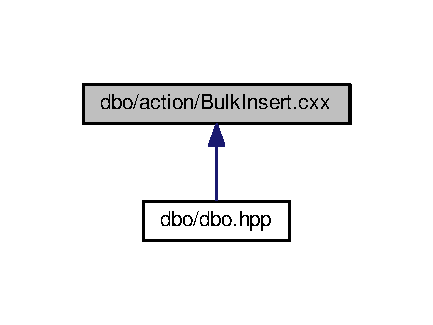
\includegraphics[width=208pt]{_bulk_insert_8cxx__dep__incl}
\end{center}
\end{figure}
\subsection*{Namespaces}
\begin{DoxyCompactItemize}
\item 
 \hyperlink{namespacedbo}{dbo}
\item 
 \hyperlink{namespacedbo_1_1action}{dbo\+::action}
\end{DoxyCompactItemize}

\hypertarget{_bulk_insert_8hpp}{\section{dbo/action/\+Bulk\+Insert.hpp File Reference}
\label{_bulk_insert_8hpp}\index{dbo/action/\+Bulk\+Insert.\+hpp@{dbo/action/\+Bulk\+Insert.\+hpp}}
}
{\ttfamily \#include $<$sstream$>$}\\*
Include dependency graph for Bulk\+Insert.\+hpp\+:\nopagebreak
\begin{figure}[H]
\begin{center}
\leavevmode
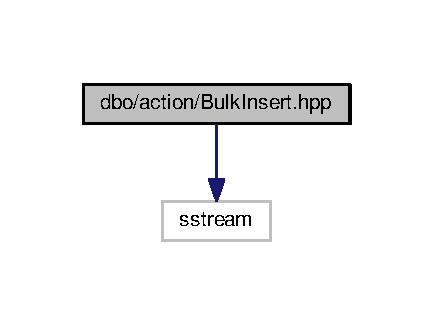
\includegraphics[width=208pt]{_bulk_insert_8hpp__incl}
\end{center}
\end{figure}
This graph shows which files directly or indirectly include this file\+:\nopagebreak
\begin{figure}[H]
\begin{center}
\leavevmode
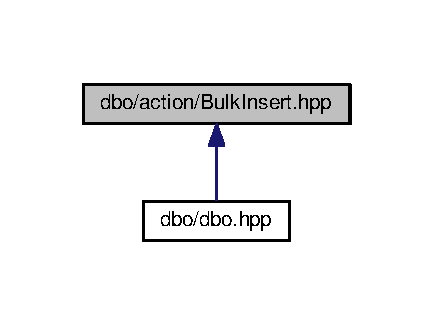
\includegraphics[width=208pt]{_bulk_insert_8hpp__dep__incl}
\end{center}
\end{figure}
\subsection*{Classes}
\begin{DoxyCompactItemize}
\item 
class \hyperlink{classdbo_1_1mapping_1_1_mapping}{dbo\+::mapping\+::\+Mapping$<$ T $>$}
\item 
class \hyperlink{classdbo_1_1mapping_1_1_field_ref}{dbo\+::mapping\+::\+Field\+Ref$<$ T $>$}
\item 
class \hyperlink{classdbo_1_1mapping_1_1_ptr_ref}{dbo\+::mapping\+::\+Ptr\+Ref$<$ T $>$}
\item 
class \hyperlink{classdbo_1_1action_1_1_bulk_insert}{dbo\+::action\+::\+Bulk\+Insert$<$ C $>$}
\end{DoxyCompactItemize}
\subsection*{Namespaces}
\begin{DoxyCompactItemize}
\item 
 \hyperlink{namespacedbo}{dbo}
\item 
 \hyperlink{namespacedbo_1_1mapping}{dbo\+::mapping}
\item 
 \hyperlink{namespacedbo_1_1action}{dbo\+::action}
\end{DoxyCompactItemize}

\hypertarget{_delete_8cxx}{\section{dbo/action/\+Delete.cxx File Reference}
\label{_delete_8cxx}\index{dbo/action/\+Delete.\+cxx@{dbo/action/\+Delete.\+cxx}}
}
This graph shows which files directly or indirectly include this file\+:\nopagebreak
\begin{figure}[H]
\begin{center}
\leavevmode
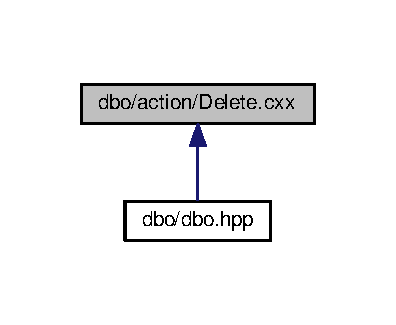
\includegraphics[width=190pt]{_delete_8cxx__dep__incl}
\end{center}
\end{figure}
\subsection*{Namespaces}
\begin{DoxyCompactItemize}
\item 
 \hyperlink{namespacedbo}{dbo}
\item 
 \hyperlink{namespacedbo_1_1action}{dbo\+::action}
\end{DoxyCompactItemize}

\hypertarget{_delete_8hpp}{\section{dbo/action/\+Delete.hpp File Reference}
\label{_delete_8hpp}\index{dbo/action/\+Delete.\+hpp@{dbo/action/\+Delete.\+hpp}}
}
This graph shows which files directly or indirectly include this file\+:\nopagebreak
\begin{figure}[H]
\begin{center}
\leavevmode
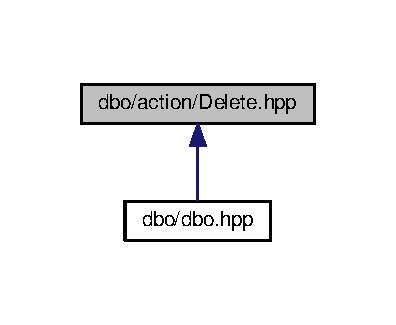
\includegraphics[width=190pt]{_delete_8hpp__dep__incl}
\end{center}
\end{figure}
\subsection*{Classes}
\begin{DoxyCompactItemize}
\item 
class \hyperlink{classdbo_1_1mapping_1_1_mapping}{dbo\+::mapping\+::\+Mapping$<$ T $>$}
\item 
class \hyperlink{classdbo_1_1mapping_1_1_field_ref}{dbo\+::mapping\+::\+Field\+Ref$<$ T $>$}
\item 
class \hyperlink{classdbo_1_1action_1_1_delete}{dbo\+::action\+::\+Delete$<$ C $>$}
\end{DoxyCompactItemize}
\subsection*{Namespaces}
\begin{DoxyCompactItemize}
\item 
 \hyperlink{namespacedbo}{dbo}
\item 
 \hyperlink{namespacedbo_1_1mapping}{dbo\+::mapping}
\item 
 \hyperlink{namespacedbo_1_1action}{dbo\+::action}
\end{DoxyCompactItemize}

\hypertarget{_init_schema_8cpp}{\section{dbo/action/\+Init\+Schema.cpp File Reference}
\label{_init_schema_8cpp}\index{dbo/action/\+Init\+Schema.\+cpp@{dbo/action/\+Init\+Schema.\+cpp}}
}
{\ttfamily \#include $<$dbo/action/\+Init\+Schema.\+hpp$>$}\\*
{\ttfamily \#include $<$dbo/mapping/\+Field.\+h$>$}\\*
{\ttfamily \#include $<$dbo/mapping/\+Field\+Info.\+h$>$}\\*
{\ttfamily \#include $<$dbo/mapping/\+Mapping\+Info.\+h$>$}\\*
Include dependency graph for Init\+Schema.\+cpp\+:\nopagebreak
\begin{figure}[H]
\begin{center}
\leavevmode
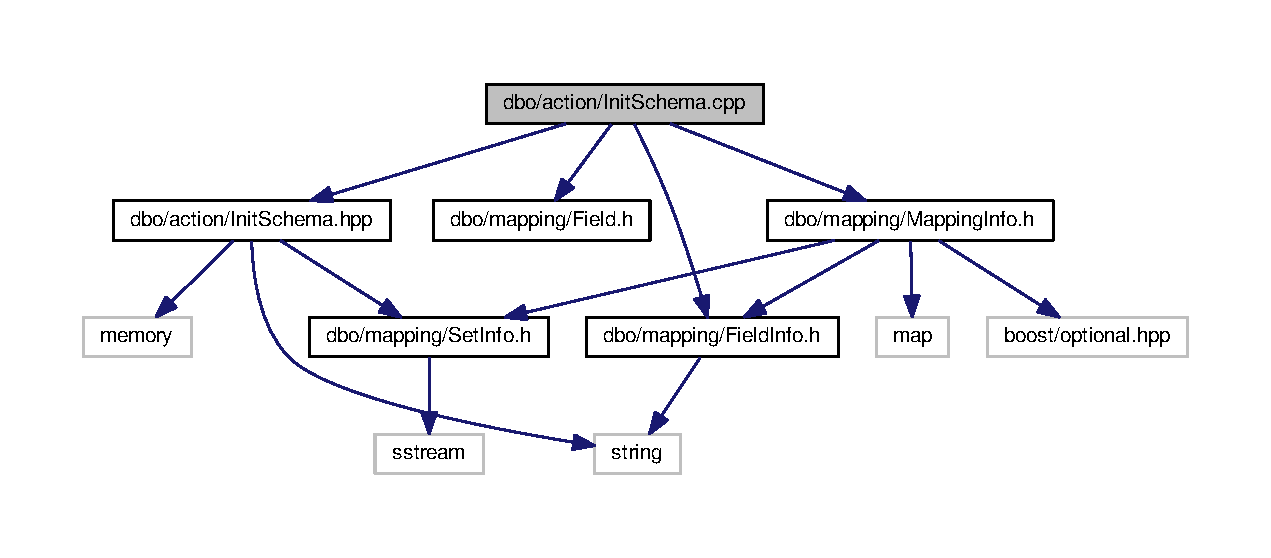
\includegraphics[width=350pt]{_init_schema_8cpp__incl}
\end{center}
\end{figure}

\hypertarget{_init_schema_8cxx}{\section{dbo/action/\+Init\+Schema.cxx File Reference}
\label{_init_schema_8cxx}\index{dbo/action/\+Init\+Schema.\+cxx@{dbo/action/\+Init\+Schema.\+cxx}}
}
{\ttfamily \#include $<$typeinfo$>$}\\*
Include dependency graph for Init\+Schema.\+cxx\+:\nopagebreak
\begin{figure}[H]
\begin{center}
\leavevmode
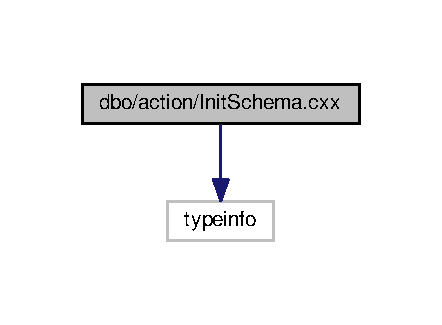
\includegraphics[width=212pt]{_init_schema_8cxx__incl}
\end{center}
\end{figure}
This graph shows which files directly or indirectly include this file\+:\nopagebreak
\begin{figure}[H]
\begin{center}
\leavevmode
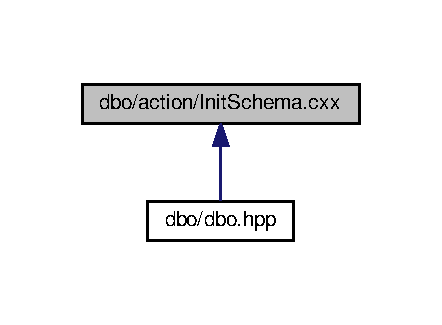
\includegraphics[width=212pt]{_init_schema_8cxx__dep__incl}
\end{center}
\end{figure}
\subsection*{Namespaces}
\begin{DoxyCompactItemize}
\item 
 \hyperlink{namespacedbo}{dbo}
\item 
 \hyperlink{namespacedbo_1_1action}{dbo\+::action}
\end{DoxyCompactItemize}

\hypertarget{_init_schema_8hpp}{\section{dbo/action/\+Init\+Schema.hpp File Reference}
\label{_init_schema_8hpp}\index{dbo/action/\+Init\+Schema.\+hpp@{dbo/action/\+Init\+Schema.\+hpp}}
}
{\ttfamily \#include $<$string$>$}\\*
{\ttfamily \#include $<$memory$>$}\\*
{\ttfamily \#include $<$dbo/mapping/\+Set\+Info.\+h$>$}\\*
Include dependency graph for Init\+Schema.\+hpp\+:\nopagebreak
\begin{figure}[H]
\begin{center}
\leavevmode
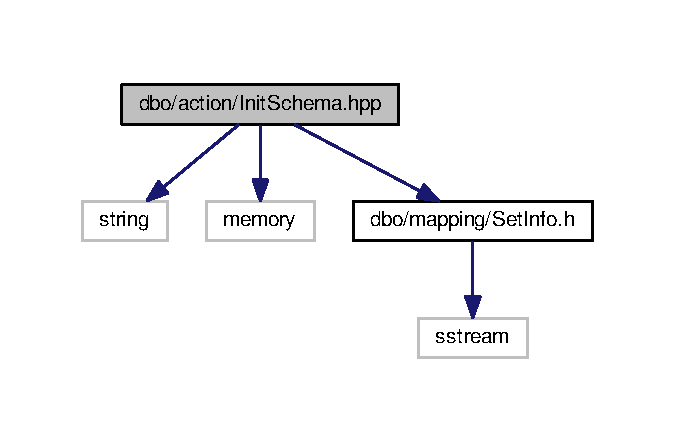
\includegraphics[width=324pt]{_init_schema_8hpp__incl}
\end{center}
\end{figure}
This graph shows which files directly or indirectly include this file\+:\nopagebreak
\begin{figure}[H]
\begin{center}
\leavevmode
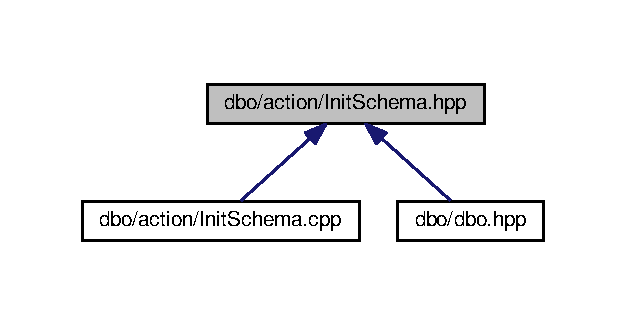
\includegraphics[width=301pt]{_init_schema_8hpp__dep__incl}
\end{center}
\end{figure}
\subsection*{Classes}
\begin{DoxyCompactItemize}
\item 
class \hyperlink{classdbo_1_1mapping_1_1_collection_ref}{dbo\+::mapping\+::\+Collection\+Ref$<$ T $>$}
\item 
class \hyperlink{classdbo_1_1mapping_1_1_field_ref}{dbo\+::mapping\+::\+Field\+Ref$<$ T $>$}
\item 
class \hyperlink{classdbo_1_1mapping_1_1_ptr_ref}{dbo\+::mapping\+::\+Ptr\+Ref$<$ T $>$}
\item 
class \hyperlink{classdbo_1_1action_1_1_init_schema}{dbo\+::action\+::\+Init\+Schema}
\end{DoxyCompactItemize}
\subsection*{Namespaces}
\begin{DoxyCompactItemize}
\item 
 \hyperlink{namespacedbo}{dbo}
\item 
 \hyperlink{namespacedbo_1_1mapping}{dbo\+::mapping}
\item 
 \hyperlink{namespacedbo_1_1action}{dbo\+::action}
\end{DoxyCompactItemize}

\hypertarget{_insert_8cxx}{\section{dbo/action/\+Insert.cxx File Reference}
\label{_insert_8cxx}\index{dbo/action/\+Insert.\+cxx@{dbo/action/\+Insert.\+cxx}}
}
This graph shows which files directly or indirectly include this file\+:\nopagebreak
\begin{figure}[H]
\begin{center}
\leavevmode
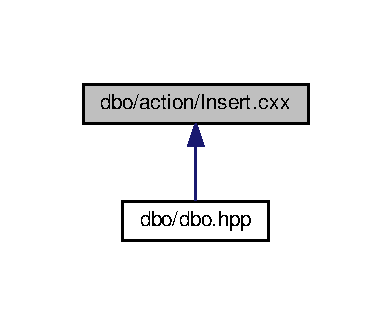
\includegraphics[width=188pt]{_insert_8cxx__dep__incl}
\end{center}
\end{figure}
\subsection*{Namespaces}
\begin{DoxyCompactItemize}
\item 
 \hyperlink{namespacedbo}{dbo}
\item 
 \hyperlink{namespacedbo_1_1action}{dbo\+::action}
\end{DoxyCompactItemize}

\hypertarget{_insert_8hpp}{\section{dbo/action/\+Insert.hpp File Reference}
\label{_insert_8hpp}\index{dbo/action/\+Insert.\+hpp@{dbo/action/\+Insert.\+hpp}}
}
This graph shows which files directly or indirectly include this file\+:\nopagebreak
\begin{figure}[H]
\begin{center}
\leavevmode
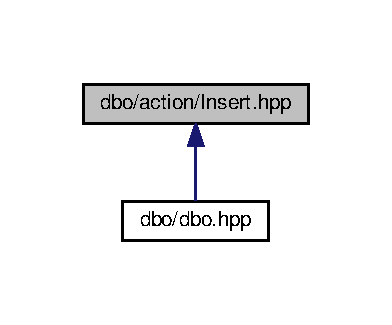
\includegraphics[width=188pt]{_insert_8hpp__dep__incl}
\end{center}
\end{figure}
\subsection*{Classes}
\begin{DoxyCompactItemize}
\item 
class \hyperlink{classdbo_1_1mapping_1_1_mapping}{dbo\+::mapping\+::\+Mapping$<$ T $>$}
\item 
class \hyperlink{classdbo_1_1mapping_1_1_field_ref}{dbo\+::mapping\+::\+Field\+Ref$<$ T $>$}
\item 
class \hyperlink{classdbo_1_1mapping_1_1_ptr_ref}{dbo\+::mapping\+::\+Ptr\+Ref$<$ T $>$}
\item 
class \hyperlink{classdbo_1_1action_1_1_insert}{dbo\+::action\+::\+Insert$<$ C $>$}
\end{DoxyCompactItemize}
\subsection*{Namespaces}
\begin{DoxyCompactItemize}
\item 
 \hyperlink{namespacedbo}{dbo}
\item 
 \hyperlink{namespacedbo_1_1mapping}{dbo\+::mapping}
\item 
 \hyperlink{namespacedbo_1_1action}{dbo\+::action}
\end{DoxyCompactItemize}

\hypertarget{_load_db_8cxx}{\section{dbo/action/\+Load\+Db.cxx File Reference}
\label{_load_db_8cxx}\index{dbo/action/\+Load\+Db.\+cxx@{dbo/action/\+Load\+Db.\+cxx}}
}
This graph shows which files directly or indirectly include this file\+:\nopagebreak
\begin{figure}[H]
\begin{center}
\leavevmode
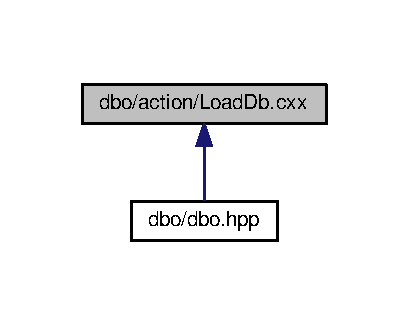
\includegraphics[width=196pt]{_load_db_8cxx__dep__incl}
\end{center}
\end{figure}
\subsection*{Namespaces}
\begin{DoxyCompactItemize}
\item 
 \hyperlink{namespacedbo}{dbo}
\item 
 \hyperlink{namespacedbo_1_1action}{dbo\+::action}
\end{DoxyCompactItemize}

\hypertarget{_load_db_8hpp}{\section{dbo/action/\+Load\+Db.hpp File Reference}
\label{_load_db_8hpp}\index{dbo/action/\+Load\+Db.\+hpp@{dbo/action/\+Load\+Db.\+hpp}}
}
This graph shows which files directly or indirectly include this file\+:\nopagebreak
\begin{figure}[H]
\begin{center}
\leavevmode
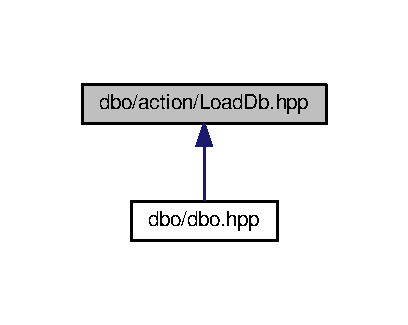
\includegraphics[width=196pt]{_load_db_8hpp__dep__incl}
\end{center}
\end{figure}
\subsection*{Classes}
\begin{DoxyCompactItemize}
\item 
class \hyperlink{classdbo_1_1mapping_1_1_mapping}{dbo\+::mapping\+::\+Mapping$<$ T $>$}
\item 
class \hyperlink{classdbo_1_1mapping_1_1_field_ref}{dbo\+::mapping\+::\+Field\+Ref$<$ T $>$}
\item 
class \hyperlink{classdbo_1_1action_1_1_load_db}{dbo\+::action\+::\+Load\+Db$<$ C $>$}
\end{DoxyCompactItemize}
\subsection*{Namespaces}
\begin{DoxyCompactItemize}
\item 
 \hyperlink{namespacedbo}{dbo}
\item 
 \hyperlink{namespacedbo_1_1mapping}{dbo\+::mapping}
\item 
 \hyperlink{namespacedbo_1_1action}{dbo\+::action}
\end{DoxyCompactItemize}

\hypertarget{_select_by_id_8cxx}{\section{dbo/action/\+Select\+By\+Id.cxx File Reference}
\label{_select_by_id_8cxx}\index{dbo/action/\+Select\+By\+Id.\+cxx@{dbo/action/\+Select\+By\+Id.\+cxx}}
}
This graph shows which files directly or indirectly include this file\+:\nopagebreak
\begin{figure}[H]
\begin{center}
\leavevmode
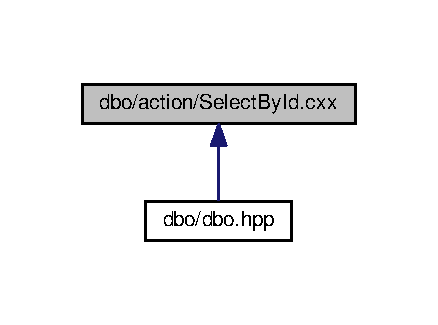
\includegraphics[width=210pt]{_select_by_id_8cxx__dep__incl}
\end{center}
\end{figure}
\subsection*{Namespaces}
\begin{DoxyCompactItemize}
\item 
 \hyperlink{namespacedbo}{dbo}
\item 
 \hyperlink{namespacedbo_1_1action}{dbo\+::action}
\end{DoxyCompactItemize}

\hypertarget{_select_by_id_8hpp}{\section{dbo/action/\+Select\+By\+Id.hpp File Reference}
\label{_select_by_id_8hpp}\index{dbo/action/\+Select\+By\+Id.\+hpp@{dbo/action/\+Select\+By\+Id.\+hpp}}
}
This graph shows which files directly or indirectly include this file\+:\nopagebreak
\begin{figure}[H]
\begin{center}
\leavevmode
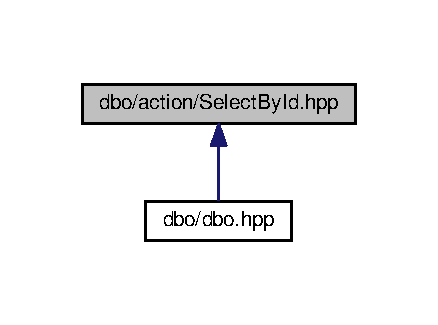
\includegraphics[width=210pt]{_select_by_id_8hpp__dep__incl}
\end{center}
\end{figure}
\subsection*{Classes}
\begin{DoxyCompactItemize}
\item 
class \hyperlink{classdbo_1_1mapping_1_1_mapping}{dbo\+::mapping\+::\+Mapping$<$ T $>$}
\item 
class \hyperlink{classdbo_1_1mapping_1_1_field_ref}{dbo\+::mapping\+::\+Field\+Ref$<$ T $>$}
\item 
class \hyperlink{classdbo_1_1action_1_1_select_by_id}{dbo\+::action\+::\+Select\+By\+Id$<$ C $>$}
\end{DoxyCompactItemize}
\subsection*{Namespaces}
\begin{DoxyCompactItemize}
\item 
 \hyperlink{namespacedbo}{dbo}
\item 
 \hyperlink{namespacedbo_1_1mapping}{dbo\+::mapping}
\item 
 \hyperlink{namespacedbo_1_1action}{dbo\+::action}
\end{DoxyCompactItemize}

\hypertarget{_update_8cxx}{\section{dbo/action/\+Update.cxx File Reference}
\label{_update_8cxx}\index{dbo/action/\+Update.\+cxx@{dbo/action/\+Update.\+cxx}}
}
This graph shows which files directly or indirectly include this file\+:\nopagebreak
\begin{figure}[H]
\begin{center}
\leavevmode
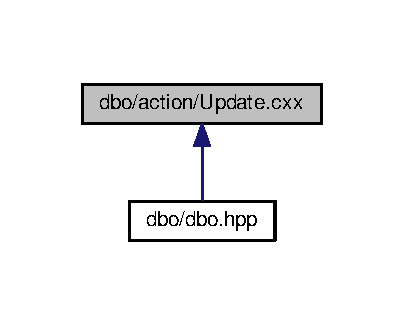
\includegraphics[width=194pt]{_update_8cxx__dep__incl}
\end{center}
\end{figure}
\subsection*{Namespaces}
\begin{DoxyCompactItemize}
\item 
 \hyperlink{namespacedbo}{dbo}
\item 
 \hyperlink{namespacedbo_1_1action}{dbo\+::action}
\end{DoxyCompactItemize}

\hypertarget{_update_8hpp}{\section{dbo/action/\+Update.hpp File Reference}
\label{_update_8hpp}\index{dbo/action/\+Update.\+hpp@{dbo/action/\+Update.\+hpp}}
}
This graph shows which files directly or indirectly include this file\+:\nopagebreak
\begin{figure}[H]
\begin{center}
\leavevmode
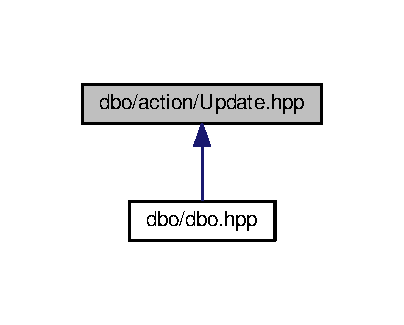
\includegraphics[width=194pt]{_update_8hpp__dep__incl}
\end{center}
\end{figure}
\subsection*{Classes}
\begin{DoxyCompactItemize}
\item 
class \hyperlink{classdbo_1_1mapping_1_1_mapping}{dbo\+::mapping\+::\+Mapping$<$ T $>$}
\item 
class \hyperlink{classdbo_1_1mapping_1_1_field_ref}{dbo\+::mapping\+::\+Field\+Ref$<$ T $>$}
\item 
class \hyperlink{classdbo_1_1action_1_1_update}{dbo\+::action\+::\+Update$<$ C $>$}
\end{DoxyCompactItemize}
\subsection*{Namespaces}
\begin{DoxyCompactItemize}
\item 
 \hyperlink{namespacedbo}{dbo}
\item 
 \hyperlink{namespacedbo_1_1mapping}{dbo\+::mapping}
\item 
 \hyperlink{namespacedbo_1_1action}{dbo\+::action}
\end{DoxyCompactItemize}

\hypertarget{collection_8cxx}{\section{dbo/collection.cxx File Reference}
\label{collection_8cxx}\index{dbo/collection.\+cxx@{dbo/collection.\+cxx}}
}
This graph shows which files directly or indirectly include this file\+:\nopagebreak
\begin{figure}[H]
\begin{center}
\leavevmode
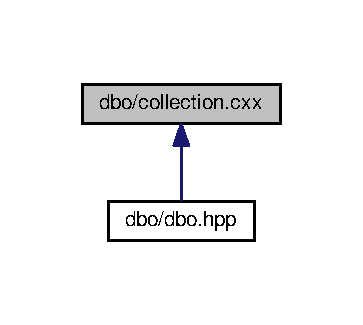
\includegraphics[width=174pt]{collection_8cxx__dep__incl}
\end{center}
\end{figure}
\subsection*{Namespaces}
\begin{DoxyCompactItemize}
\item 
 \hyperlink{namespacedbo}{dbo}
\end{DoxyCompactItemize}

\hypertarget{collection_8hpp}{\section{dbo/collection.hpp File Reference}
\label{collection_8hpp}\index{dbo/collection.\+hpp@{dbo/collection.\+hpp}}
}
{\ttfamily \#include $<$deque$>$}\\*
Include dependency graph for collection.\+hpp\+:\nopagebreak
\begin{figure}[H]
\begin{center}
\leavevmode
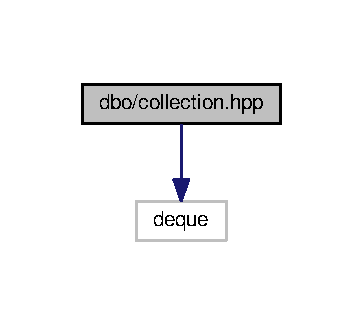
\includegraphics[width=174pt]{collection_8hpp__incl}
\end{center}
\end{figure}
This graph shows which files directly or indirectly include this file\+:\nopagebreak
\begin{figure}[H]
\begin{center}
\leavevmode
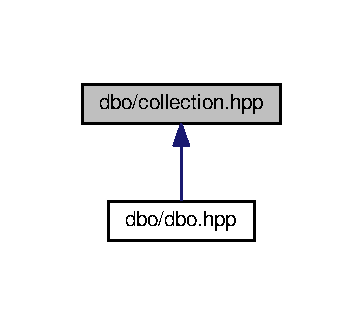
\includegraphics[width=174pt]{collection_8hpp__dep__incl}
\end{center}
\end{figure}
\subsection*{Classes}
\begin{DoxyCompactItemize}
\item 
class \hyperlink{classdbo_1_1ptr}{dbo\+::ptr$<$ C $>$}
\item 
class \hyperlink{classdbo_1_1collection}{dbo\+::collection$<$ C $>$}
\item 
class \hyperlink{classdbo_1_1collection_1_1iterator}{dbo\+::collection$<$ C $>$\+::iterator}
\end{DoxyCompactItemize}
\subsection*{Namespaces}
\begin{DoxyCompactItemize}
\item 
 \hyperlink{namespacedbo}{dbo}
\end{DoxyCompactItemize}

\hypertarget{connection_8cpp}{\section{dbo/connection.cpp File Reference}
\label{connection_8cpp}\index{dbo/connection.\+cpp@{dbo/connection.\+cpp}}
}
{\ttfamily \#include $<$dbo/connection.\+h$>$}\\*
{\ttfamily \#include $<$dbo/mapping/\+Field.\+h$>$}\\*
{\ttfamily \#include $<$dbo/mapping/\+Field\+Info.\+h$>$}\\*
{\ttfamily \#include $<$dbo/mapping/\+Set\+Info.\+h$>$}\\*
{\ttfamily \#include $<$dbo/mapping/\+Mapping\+Info.\+h$>$}\\*
{\ttfamily \#include $<$dbo/mapping/\+Mapping.\+hpp$>$}\\*
{\ttfamily \#include $<$dbo/stmt/\+Prepared\+Statement.\+h$>$}\\*
{\ttfamily \#include $<$dbo/traits/sql\+\_\+value\+\_\+traits.\+hpp$>$}\\*
{\ttfamily \#include $<$dbo/traits/\+Std\+Sql\+Traits.\+h$>$}\\*
{\ttfamily \#include $<$postgresql/libpq-\/fe.\+h$>$}\\*
Include dependency graph for connection.\+cpp\+:\nopagebreak
\begin{figure}[H]
\begin{center}
\leavevmode
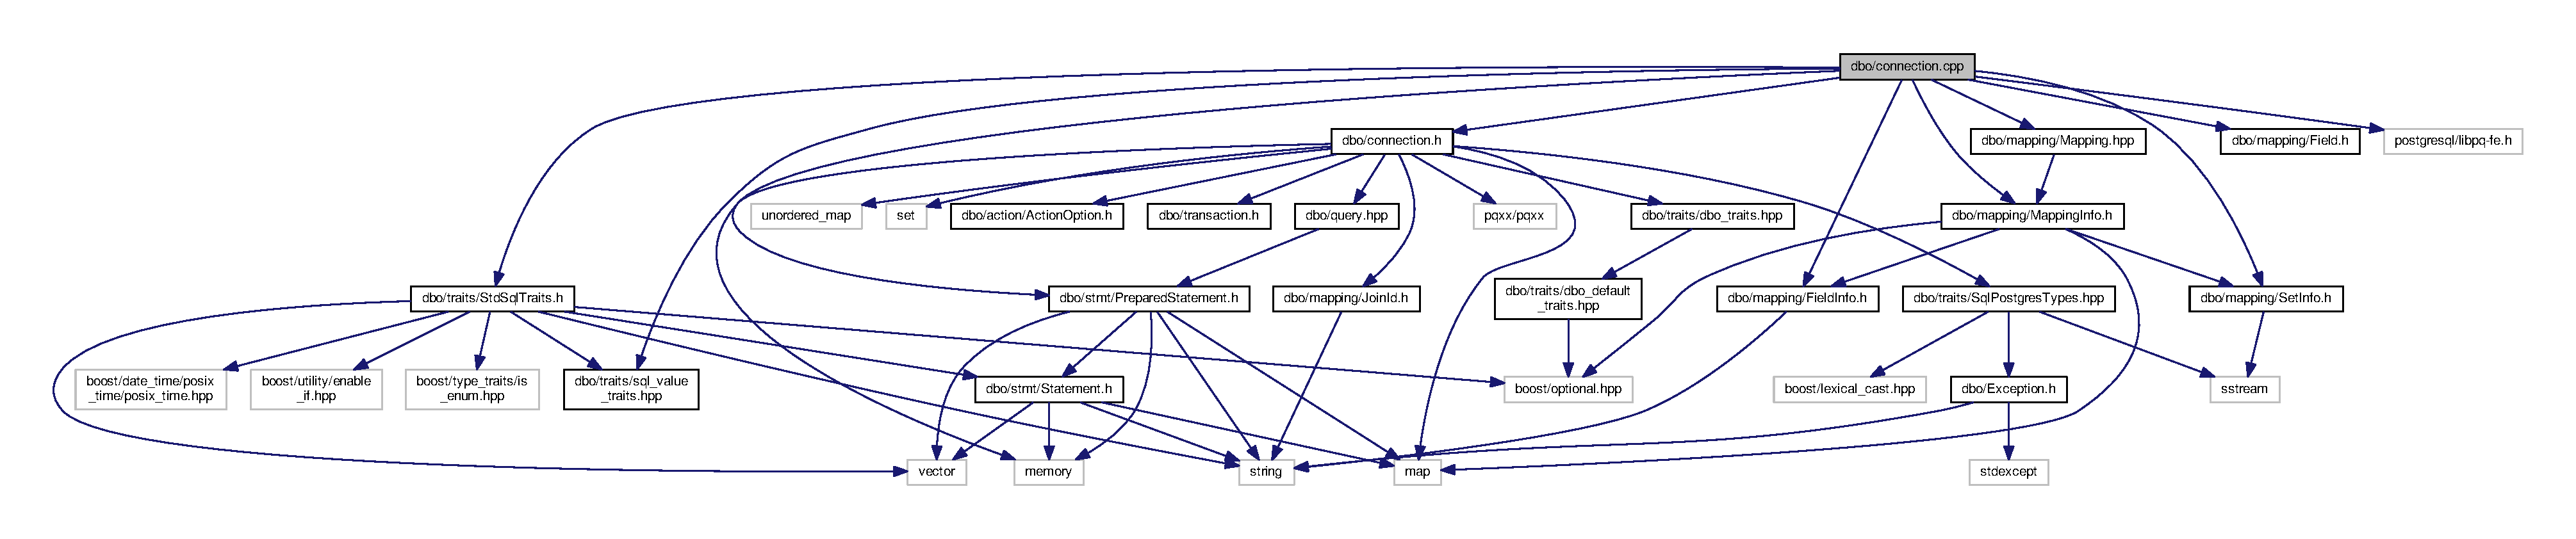
\includegraphics[width=350pt]{connection_8cpp__incl}
\end{center}
\end{figure}
\subsection*{Functions}
\begin{DoxyCompactItemize}
\item 
std\+::string \& \hyperlink{connection_8cpp_ace4f7ce47eb184086c37bc588d168614}{replace} (std\+::string \&s, char c, const std\+::string \&r)
\item 
std\+::string \hyperlink{connection_8cpp_a1d5792fcb599079e1a716f36ef92b493}{quote\+Schema\+Dot} (const std\+::string \&table)
\end{DoxyCompactItemize}


\subsection{Function Documentation}
\hypertarget{connection_8cpp_a1d5792fcb599079e1a716f36ef92b493}{\index{connection.\+cpp@{connection.\+cpp}!quote\+Schema\+Dot@{quote\+Schema\+Dot}}
\index{quote\+Schema\+Dot@{quote\+Schema\+Dot}!connection.\+cpp@{connection.\+cpp}}
\subsubsection[{quote\+Schema\+Dot}]{\setlength{\rightskip}{0pt plus 5cm}std\+::string quote\+Schema\+Dot (
\begin{DoxyParamCaption}
\item[{const std\+::string \&}]{table}
\end{DoxyParamCaption}
)}}\label{connection_8cpp_a1d5792fcb599079e1a716f36ef92b493}
\hypertarget{connection_8cpp_ace4f7ce47eb184086c37bc588d168614}{\index{connection.\+cpp@{connection.\+cpp}!replace@{replace}}
\index{replace@{replace}!connection.\+cpp@{connection.\+cpp}}
\subsubsection[{replace}]{\setlength{\rightskip}{0pt plus 5cm}std\+::string\& replace (
\begin{DoxyParamCaption}
\item[{std\+::string \&}]{s, }
\item[{char}]{c, }
\item[{const std\+::string \&}]{r}
\end{DoxyParamCaption}
)}}\label{connection_8cpp_ace4f7ce47eb184086c37bc588d168614}

\hypertarget{connection_8cxx}{\section{dbo/connection.cxx File Reference}
\label{connection_8cxx}\index{dbo/connection.\+cxx@{dbo/connection.\+cxx}}
}
This graph shows which files directly or indirectly include this file\+:\nopagebreak
\begin{figure}[H]
\begin{center}
\leavevmode
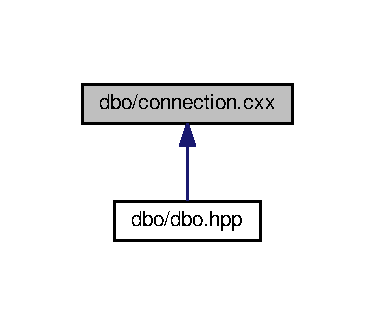
\includegraphics[width=180pt]{connection_8cxx__dep__incl}
\end{center}
\end{figure}
\subsection*{Namespaces}
\begin{DoxyCompactItemize}
\item 
 \hyperlink{namespacedbo}{dbo}
\end{DoxyCompactItemize}

\hypertarget{connection_8h}{\section{dbo/connection.h File Reference}
\label{connection_8h}\index{dbo/connection.\+h@{dbo/connection.\+h}}
}
{\ttfamily \#include $<$unordered\+\_\+map$>$}\\*
{\ttfamily \#include $<$map$>$}\\*
{\ttfamily \#include $<$memory$>$}\\*
{\ttfamily \#include $<$set$>$}\\*
{\ttfamily \#include $<$dbo/action/\+Action\+Option.\+h$>$}\\*
{\ttfamily \#include $<$dbo/mapping/\+Join\+Id.\+h$>$}\\*
{\ttfamily \#include $<$dbo/traits/\+Sql\+Postgres\+Types.\+hpp$>$}\\*
{\ttfamily \#include $<$dbo/traits/dbo\+\_\+traits.\+hpp$>$}\\*
{\ttfamily \#include $<$dbo/transaction.\+h$>$}\\*
{\ttfamily \#include $<$dbo/query.\+hpp$>$}\\*
{\ttfamily \#include $<$pqxx/pqxx$>$}\\*
Include dependency graph for connection.\+h\+:\nopagebreak
\begin{figure}[H]
\begin{center}
\leavevmode
\includegraphics[width=350pt]{connection_8h__incl}
\end{center}
\end{figure}
This graph shows which files directly or indirectly include this file\+:\nopagebreak
\begin{figure}[H]
\begin{center}
\leavevmode
\includegraphics[width=350pt]{connection_8h__dep__incl}
\end{center}
\end{figure}
\subsection*{Classes}
\begin{DoxyCompactItemize}
\item 
class \hyperlink{classdbo_1_1collection}{dbo\+::collection$<$ C $>$}
\item 
class \hyperlink{classdbo_1_1ptr}{dbo\+::ptr$<$ C $>$}
\item 
class \hyperlink{classdbo_1_1action_1_1_delete}{dbo\+::action\+::\+Delete$<$ C $>$}
\item 
class \hyperlink{classdbo_1_1action_1_1_insert}{dbo\+::action\+::\+Insert$<$ C $>$}
\item 
class \hyperlink{classdbo_1_1action_1_1_select_by_id}{dbo\+::action\+::\+Select\+By\+Id$<$ C $>$}
\item 
class \hyperlink{classdbo_1_1action_1_1_update}{dbo\+::action\+::\+Update$<$ C $>$}
\item 
class \hyperlink{classdbo_1_1mapping_1_1_mapping}{dbo\+::mapping\+::\+Mapping$<$ T $>$}
\item 
class \hyperlink{classdbo_1_1mapping_1_1_ptr_ref}{dbo\+::mapping\+::\+Ptr\+Ref$<$ T $>$}
\item 
class \hyperlink{classdbo_1_1connection}{dbo\+::connection}
\item 
struct \hyperlink{structdbo_1_1connection_1_1typecomp}{dbo\+::connection\+::typecomp}
\end{DoxyCompactItemize}
\subsection*{Namespaces}
\begin{DoxyCompactItemize}
\item 
 \hyperlink{namespacedbo}{dbo}
\item 
 \hyperlink{namespacedbo_1_1action}{dbo\+::action}
\item 
 \hyperlink{namespacedbo_1_1mapping}{dbo\+::mapping}
\item 
 \hyperlink{namespacedbo_1_1stmt}{dbo\+::stmt}
\end{DoxyCompactItemize}
\subsection*{Typedefs}
\begin{DoxyCompactItemize}
\item 
typedef struct pg\+\_\+conn \hyperlink{connection_8h_a5ed62e34058025c39959695e724603a6}{P\+Gconn}
\end{DoxyCompactItemize}


\subsection{Typedef Documentation}
\hypertarget{connection_8h_a5ed62e34058025c39959695e724603a6}{\index{connection.\+h@{connection.\+h}!P\+Gconn@{P\+Gconn}}
\index{P\+Gconn@{P\+Gconn}!connection.\+h@{connection.\+h}}
\subsubsection[{P\+Gconn}]{\setlength{\rightskip}{0pt plus 5cm}typedef struct pg\+\_\+conn {\bf P\+Gconn}}}\label{connection_8h_a5ed62e34058025c39959695e724603a6}

\hypertarget{dbo_8hpp}{\section{dbo/dbo.hpp File Reference}
\label{dbo_8hpp}\index{dbo/dbo.\+hpp@{dbo/dbo.\+hpp}}
}
{\ttfamily \#include $<$csignal$>$}\\*
{\ttfamily \#include $<$dbo/connection.\+h$>$}\\*
{\ttfamily \#include $<$dbo/ptr.\+hpp$>$}\\*
{\ttfamily \#include $<$dbo/collection.\+hpp$>$}\\*
{\ttfamily \#include $<$dbo/relation.\+hpp$>$}\\*
{\ttfamily \#include $<$dbo/query.\+hpp$>$}\\*
{\ttfamily \#include $<$dbo/\+Exception.\+h$>$}\\*
{\ttfamily \#include $<$dbo/stmt/\+Bulk\+Statement.\+h$>$}\\*
{\ttfamily \#include $<$dbo/stmt/\+Prepared\+Statement.\+h$>$}\\*
{\ttfamily \#include $<$dbo/traits/dbo\+\_\+traits.\+hpp$>$}\\*
{\ttfamily \#include $<$dbo/traits/\+Std\+Sql\+Traits.\+h$>$}\\*
{\ttfamily \#include $<$dbo/mapping/\+Mapping.\+hpp$>$}\\*
{\ttfamily \#include $<$dbo/mapping/\+Collection\+Ref.\+hpp$>$}\\*
{\ttfamily \#include $<$dbo/mapping/\+Field\+Ref.\+hpp$>$}\\*
{\ttfamily \#include $<$dbo/mapping/\+Ptr\+Ref.\+hpp$>$}\\*
{\ttfamily \#include $<$dbo/action/\+Init\+Schema.\+hpp$>$}\\*
{\ttfamily \#include $<$dbo/action/\+Delete.\+hpp$>$}\\*
{\ttfamily \#include $<$dbo/action/\+Bulk\+Insert.\+hpp$>$}\\*
{\ttfamily \#include $<$dbo/action/\+Insert.\+hpp$>$}\\*
{\ttfamily \#include $<$dbo/action/\+Update.\+hpp$>$}\\*
{\ttfamily \#include $<$dbo/action/\+Select\+By\+Id.\+hpp$>$}\\*
{\ttfamily \#include $<$dbo/action/\+Load\+Db.\+hpp$>$}\\*
{\ttfamily \#include $<$dbo/connection.\+cxx$>$}\\*
{\ttfamily \#include $<$dbo/ptr.\+cxx$>$}\\*
{\ttfamily \#include $<$dbo/collection.\+cxx$>$}\\*
{\ttfamily \#include $<$dbo/relation.\+cxx$>$}\\*
{\ttfamily \#include $<$dbo/query.\+cxx$>$}\\*
{\ttfamily \#include $<$dbo/action/\+Init\+Schema.\+cxx$>$}\\*
{\ttfamily \#include $<$dbo/action/\+Delete.\+cxx$>$}\\*
{\ttfamily \#include $<$dbo/action/\+Bulk\+Insert.\+cxx$>$}\\*
{\ttfamily \#include $<$dbo/action/\+Insert.\+cxx$>$}\\*
{\ttfamily \#include $<$dbo/action/\+Update.\+cxx$>$}\\*
{\ttfamily \#include $<$dbo/action/\+Select\+By\+Id.\+cxx$>$}\\*
{\ttfamily \#include $<$dbo/action/\+Load\+Db.\+cxx$>$}\\*
{\ttfamily \#include $<$dbo/mapping/\+Field\+Ref.\+cxx$>$}\\*
{\ttfamily \#include $<$dbo/mapping/\+Ptr\+Ref.\+cxx$>$}\\*
{\ttfamily \#include $<$dbo/mapping/\+Mapping.\+cxx$>$}\\*
Include dependency graph for dbo.\+hpp\+:\nopagebreak
\begin{figure}[H]
\begin{center}
\leavevmode
\includegraphics[width=350pt]{dbo_8hpp__incl}
\end{center}
\end{figure}

\hypertarget{_exception_8h}{\section{dbo/\+Exception.h File Reference}
\label{_exception_8h}\index{dbo/\+Exception.\+h@{dbo/\+Exception.\+h}}
}
{\ttfamily \#include $<$string$>$}\\*
{\ttfamily \#include $<$stdexcept$>$}\\*
Include dependency graph for Exception.\+h\+:\nopagebreak
\begin{figure}[H]
\begin{center}
\leavevmode
\includegraphics[width=197pt]{_exception_8h__incl}
\end{center}
\end{figure}
This graph shows which files directly or indirectly include this file\+:\nopagebreak
\begin{figure}[H]
\begin{center}
\leavevmode
\includegraphics[width=350pt]{_exception_8h__dep__incl}
\end{center}
\end{figure}
\subsection*{Classes}
\begin{DoxyCompactItemize}
\item 
class \hyperlink{classdbo_1_1_exception}{dbo\+::\+Exception}
\end{DoxyCompactItemize}
\subsection*{Namespaces}
\begin{DoxyCompactItemize}
\item 
 \hyperlink{namespacedbo}{dbo}
\end{DoxyCompactItemize}

\hypertarget{_collection_ref_8hpp}{\section{dbo/mapping/\+Collection\+Ref.hpp File Reference}
\label{_collection_ref_8hpp}\index{dbo/mapping/\+Collection\+Ref.\+hpp@{dbo/mapping/\+Collection\+Ref.\+hpp}}
}
This graph shows which files directly or indirectly include this file\+:\nopagebreak
\begin{figure}[H]
\begin{center}
\leavevmode
\includegraphics[width=232pt]{_collection_ref_8hpp__dep__incl}
\end{center}
\end{figure}
\subsection*{Classes}
\begin{DoxyCompactItemize}
\item 
class \hyperlink{classdbo_1_1mapping_1_1_collection_ref}{dbo\+::mapping\+::\+Collection\+Ref$<$ T $>$}
\end{DoxyCompactItemize}
\subsection*{Namespaces}
\begin{DoxyCompactItemize}
\item 
 \hyperlink{namespacedbo}{dbo}
\item 
 \hyperlink{namespacedbo_1_1mapping}{dbo\+::mapping}
\end{DoxyCompactItemize}

\hypertarget{_field_8h}{\section{dbo/mapping/\+Field.h File Reference}
\label{_field_8h}\index{dbo/mapping/\+Field.\+h@{dbo/mapping/\+Field.\+h}}
}
This graph shows which files directly or indirectly include this file\+:\nopagebreak
\begin{figure}[H]
\begin{center}
\leavevmode
\includegraphics[width=331pt]{_field_8h__dep__incl}
\end{center}
\end{figure}
\subsection*{Namespaces}
\begin{DoxyCompactItemize}
\item 
 \hyperlink{namespacedbo}{dbo}
\item 
 \hyperlink{namespacedbo_1_1mapping}{dbo\+::mapping}
\end{DoxyCompactItemize}
\subsection*{Variables}
\begin{DoxyCompactItemize}
\item 
const int \hyperlink{namespacedbo_1_1mapping_a524c2de86b4169d431af199d866f8331}{dbo\+::mapping\+::\+F\+K\+Not\+Null} = 0x01
\item 
const int \hyperlink{namespacedbo_1_1mapping_a49684099001aa562bd3f41e20d9130ca}{dbo\+::mapping\+::\+F\+K\+On\+Update\+Cascade} = 0x02
\item 
const int \hyperlink{namespacedbo_1_1mapping_a382d00e9ad29bb1d14533bf44579ed9b}{dbo\+::mapping\+::\+F\+K\+On\+Update\+Set\+Null} = 0x04
\item 
const int \hyperlink{namespacedbo_1_1mapping_af0f560be1c6628c4332af57fd0a9890e}{dbo\+::mapping\+::\+F\+K\+On\+Delete\+Cascade} = 0x08
\item 
const int \hyperlink{namespacedbo_1_1mapping_ab82b6560e26b4e5d430a4c250bd9ff24}{dbo\+::mapping\+::\+F\+K\+On\+Delete\+Set\+Null} = 0x10
\end{DoxyCompactItemize}

\hypertarget{_field_info_8cpp}{\section{dbo/mapping/\+Field\+Info.cpp File Reference}
\label{_field_info_8cpp}\index{dbo/mapping/\+Field\+Info.\+cpp@{dbo/mapping/\+Field\+Info.\+cpp}}
}
{\ttfamily \#include $<$dbo/mapping/\+Field\+Info.\+h$>$}\\*
{\ttfamily \#include $<$sstream$>$}\\*
{\ttfamily \#include $<$typeinfo$>$}\\*
Include dependency graph for Field\+Info.\+cpp\+:\nopagebreak
\begin{figure}[H]
\begin{center}
\leavevmode
\includegraphics[width=340pt]{_field_info_8cpp__incl}
\end{center}
\end{figure}

\hypertarget{_field_info_8h}{\section{dbo/mapping/\+Field\+Info.h File Reference}
\label{_field_info_8h}\index{dbo/mapping/\+Field\+Info.\+h@{dbo/mapping/\+Field\+Info.\+h}}
}
{\ttfamily \#include $<$string$>$}\\*
Include dependency graph for Field\+Info.\+h\+:\nopagebreak
\begin{figure}[H]
\begin{center}
\leavevmode
\includegraphics[width=200pt]{_field_info_8h__incl}
\end{center}
\end{figure}
This graph shows which files directly or indirectly include this file\+:\nopagebreak
\begin{figure}[H]
\begin{center}
\leavevmode
\includegraphics[width=350pt]{_field_info_8h__dep__incl}
\end{center}
\end{figure}
\subsection*{Classes}
\begin{DoxyCompactItemize}
\item 
class \hyperlink{classdbo_1_1mapping_1_1_field_info}{dbo\+::mapping\+::\+Field\+Info}
\begin{DoxyCompactList}\small\item\em Description of a field. \end{DoxyCompactList}\end{DoxyCompactItemize}
\subsection*{Namespaces}
\begin{DoxyCompactItemize}
\item 
 \hyperlink{namespacedbo}{dbo}
\item 
 \hyperlink{namespacedbo_1_1mapping}{dbo\+::mapping}
\end{DoxyCompactItemize}

\hypertarget{_field_ref_8cxx}{\section{dbo/mapping/\+Field\+Ref.cxx File Reference}
\label{_field_ref_8cxx}\index{dbo/mapping/\+Field\+Ref.\+cxx@{dbo/mapping/\+Field\+Ref.\+cxx}}
}
{\ttfamily \#include $<$typeinfo$>$}\\*
Include dependency graph for Field\+Ref.\+cxx\+:\nopagebreak
\begin{figure}[H]
\begin{center}
\leavevmode
\includegraphics[width=210pt]{_field_ref_8cxx__incl}
\end{center}
\end{figure}
This graph shows which files directly or indirectly include this file\+:\nopagebreak
\begin{figure}[H]
\begin{center}
\leavevmode
\includegraphics[width=210pt]{_field_ref_8cxx__dep__incl}
\end{center}
\end{figure}
\subsection*{Namespaces}
\begin{DoxyCompactItemize}
\item 
 \hyperlink{namespacedbo}{dbo}
\item 
 \hyperlink{namespacedbo_1_1mapping}{dbo\+::mapping}
\end{DoxyCompactItemize}

\hypertarget{_field_ref_8hpp}{\section{dbo/mapping/\+Field\+Ref.hpp File Reference}
\label{_field_ref_8hpp}\index{dbo/mapping/\+Field\+Ref.\+hpp@{dbo/mapping/\+Field\+Ref.\+hpp}}
}
This graph shows which files directly or indirectly include this file\+:\nopagebreak
\begin{figure}[H]
\begin{center}
\leavevmode
\includegraphics[width=210pt]{_field_ref_8hpp__dep__incl}
\end{center}
\end{figure}
\subsection*{Classes}
\begin{DoxyCompactItemize}
\item 
class \hyperlink{classdbo_1_1mapping_1_1_field_ref}{dbo\+::mapping\+::\+Field\+Ref$<$ T $>$}
\end{DoxyCompactItemize}
\subsection*{Namespaces}
\begin{DoxyCompactItemize}
\item 
 \hyperlink{namespacedbo}{dbo}
\item 
 \hyperlink{namespacedbo_1_1mapping}{dbo\+::mapping}
\end{DoxyCompactItemize}

\hypertarget{_foreign_key_constraint_8cpp}{\section{dbo/mapping/\+Foreign\+Key\+Constraint.cpp File Reference}
\label{_foreign_key_constraint_8cpp}\index{dbo/mapping/\+Foreign\+Key\+Constraint.\+cpp@{dbo/mapping/\+Foreign\+Key\+Constraint.\+cpp}}
}
{\ttfamily \#include $<$dbo/mapping/\+Foreign\+Key\+Constraint.\+h$>$}\\*
Include dependency graph for Foreign\+Key\+Constraint.\+cpp\+:\nopagebreak
\begin{figure}[H]
\begin{center}
\leavevmode
\includegraphics[width=268pt]{_foreign_key_constraint_8cpp__incl}
\end{center}
\end{figure}

\hypertarget{_foreign_key_constraint_8h}{\section{dbo/mapping/\+Foreign\+Key\+Constraint.h File Reference}
\label{_foreign_key_constraint_8h}\index{dbo/mapping/\+Foreign\+Key\+Constraint.\+h@{dbo/mapping/\+Foreign\+Key\+Constraint.\+h}}
}
This graph shows which files directly or indirectly include this file\+:\nopagebreak
\begin{figure}[H]
\begin{center}
\leavevmode
\includegraphics[width=350pt]{_foreign_key_constraint_8h__dep__incl}
\end{center}
\end{figure}
\subsection*{Classes}
\begin{DoxyCompactItemize}
\item 
class \hyperlink{classdbo_1_1_foreign_key_constraint}{dbo\+::\+Foreign\+Key\+Constraint}
\end{DoxyCompactItemize}
\subsection*{Namespaces}
\begin{DoxyCompactItemize}
\item 
 \hyperlink{namespacedbo}{dbo}
\item 
 \hyperlink{namespacedbo_1_1fk}{dbo\+::fk}
\end{DoxyCompactItemize}
\subsection*{Functions}
\begin{DoxyCompactItemize}
\item 
\hyperlink{classdbo_1_1_foreign_key_constraint}{Foreign\+Key\+Constraint} \hyperlink{namespacedbo_ae5bf60d97447a53872534069944ba4a7}{dbo\+::operator$\vert$} (\hyperlink{classdbo_1_1_foreign_key_constraint}{Foreign\+Key\+Constraint} lhs, \hyperlink{classdbo_1_1_foreign_key_constraint}{Foreign\+Key\+Constraint} rhs)
\begin{DoxyCompactList}\small\item\em Combines two constraints. \end{DoxyCompactList}\item 
const Foreign\+Key\+Constraint \hyperlink{namespacedbo_1_1fk_a074c2f3bc21f375877f9b6b67710c848}{dbo\+::fk\+::\+None} (F\+K\+None)
\begin{DoxyCompactList}\small\item\em A constraint that prevents a {\ttfamily null} ptr. \end{DoxyCompactList}\item 
const Foreign\+Key\+Constraint \hyperlink{namespacedbo_1_1fk_ad0d91eae612ebf7978662e948c5c4363}{dbo\+::fk\+::\+Not\+Null} (F\+K\+Not\+Null)
\begin{DoxyCompactList}\small\item\em A constraint that prevents a {\ttfamily null} ptr. \end{DoxyCompactList}\item 
const Foreign\+Key\+Constraint \hyperlink{namespacedbo_1_1fk_a00c09046d5885af90f78fdb0ffbc751d}{dbo\+::fk\+::\+On\+Update\+Cascade} (F\+K\+On\+Update\+Cascade)
\begin{DoxyCompactList}\small\item\em A constraint that cascades updates. \end{DoxyCompactList}\item 
const Foreign\+Key\+Constraint \hyperlink{namespacedbo_1_1fk_adcedfa8d9519fac76fe9b74185c6a078}{dbo\+::fk\+::\+On\+Update\+Set\+Null} (F\+K\+On\+Update\+Set\+Null)
\begin{DoxyCompactList}\small\item\em A constraint that cascades updates. \end{DoxyCompactList}\item 
const Foreign\+Key\+Constraint \hyperlink{namespacedbo_1_1fk_a134bc7a078790f346ee7968529d1957e}{dbo\+::fk\+::\+On\+Delete\+Cascade} (F\+K\+On\+Delete\+Cascade)
\begin{DoxyCompactList}\small\item\em A constraint that cascades deletes. \end{DoxyCompactList}\item 
const Foreign\+Key\+Constraint \hyperlink{namespacedbo_1_1fk_af99903fe2691e999c217d3811d1e8678}{dbo\+::fk\+::\+On\+Delete\+Set\+Null} (F\+K\+On\+Delete\+Set\+Null)
\begin{DoxyCompactList}\small\item\em A constraint that cascades deletes. \end{DoxyCompactList}\end{DoxyCompactItemize}
\subsection*{Variables}
\begin{DoxyCompactItemize}
\item 
const int \hyperlink{namespacedbo_a852726cb6e354fe0b7427952d7ee9bbd}{dbo\+::\+F\+K\+None} =0x00
\item 
const int \hyperlink{namespacedbo_aaee974161f0dade23c6dbd3aa44a145b}{dbo\+::\+F\+K\+Not\+Null} =0x01
\item 
const int \hyperlink{namespacedbo_ad015d5bfa1c6cfd1efbb7b6e97eb22ae}{dbo\+::\+F\+K\+On\+Update\+Cascade} =0x02
\item 
const int \hyperlink{namespacedbo_ac28416e0d117ea1806ceee4558b0f96b}{dbo\+::\+F\+K\+On\+Update\+Set\+Null} =0x04
\item 
const int \hyperlink{namespacedbo_a58edf54e3f9cb2c68130845cb2cff826}{dbo\+::\+F\+K\+On\+Delete\+Cascade} =0x08
\item 
const int \hyperlink{namespacedbo_ad8a98b325ad0becbd7231e924c6dbe26}{dbo\+::\+F\+K\+On\+Delete\+Set\+Null} =0x10
\end{DoxyCompactItemize}

\hypertarget{_join_id_8cpp}{\section{dbo/mapping/\+Join\+Id.cpp File Reference}
\label{_join_id_8cpp}\index{dbo/mapping/\+Join\+Id.\+cpp@{dbo/mapping/\+Join\+Id.\+cpp}}
}
{\ttfamily \#include $<$dbo/mapping/\+Join\+Id.\+h$>$}\\*
Include dependency graph for Join\+Id.\+cpp\+:\nopagebreak
\begin{figure}[H]
\begin{center}
\leavevmode
\includegraphics[width=198pt]{_join_id_8cpp__incl}
\end{center}
\end{figure}
\subsection*{Namespaces}
\begin{DoxyCompactItemize}
\item 
 \hyperlink{namespacedbo}{dbo}
\item 
 \hyperlink{namespacedbo_1_1mapping}{dbo\+::mapping}
\end{DoxyCompactItemize}

\hypertarget{_join_id_8h}{\section{dbo/mapping/\+Join\+Id.h File Reference}
\label{_join_id_8h}\index{dbo/mapping/\+Join\+Id.\+h@{dbo/mapping/\+Join\+Id.\+h}}
}
{\ttfamily \#include $<$string$>$}\\*
Include dependency graph for Join\+Id.\+h\+:\nopagebreak
\begin{figure}[H]
\begin{center}
\leavevmode
\includegraphics[width=190pt]{_join_id_8h__incl}
\end{center}
\end{figure}
This graph shows which files directly or indirectly include this file\+:\nopagebreak
\begin{figure}[H]
\begin{center}
\leavevmode
\includegraphics[width=350pt]{_join_id_8h__dep__incl}
\end{center}
\end{figure}
\subsection*{Classes}
\begin{DoxyCompactItemize}
\item 
struct \hyperlink{structdbo_1_1mapping_1_1_join_id}{dbo\+::mapping\+::\+Join\+Id}
\end{DoxyCompactItemize}
\subsection*{Namespaces}
\begin{DoxyCompactItemize}
\item 
 \hyperlink{namespacedbo}{dbo}
\item 
 \hyperlink{namespacedbo_1_1mapping}{dbo\+::mapping}
\end{DoxyCompactItemize}

\hypertarget{_mapping_8cxx}{\section{dbo/mapping/\+Mapping.cxx File Reference}
\label{_mapping_8cxx}\index{dbo/mapping/\+Mapping.\+cxx@{dbo/mapping/\+Mapping.\+cxx}}
}
{\ttfamily \#include $<$boost/type\+\_\+traits/remove\+\_\+const.\+hpp$>$}\\*
Include dependency graph for Mapping.\+cxx\+:\nopagebreak
\begin{figure}[H]
\begin{center}
\leavevmode
\includegraphics[width=210pt]{_mapping_8cxx__incl}
\end{center}
\end{figure}
This graph shows which files directly or indirectly include this file\+:\nopagebreak
\begin{figure}[H]
\begin{center}
\leavevmode
\includegraphics[width=210pt]{_mapping_8cxx__dep__incl}
\end{center}
\end{figure}
\subsection*{Namespaces}
\begin{DoxyCompactItemize}
\item 
 \hyperlink{namespacedbo}{dbo}
\item 
 \hyperlink{namespacedbo_1_1mapping}{dbo\+::mapping}
\end{DoxyCompactItemize}

\hypertarget{_mapping_8hpp}{\section{dbo/mapping/\+Mapping.hpp File Reference}
\label{_mapping_8hpp}\index{dbo/mapping/\+Mapping.\+hpp@{dbo/mapping/\+Mapping.\+hpp}}
}
{\ttfamily \#include $<$dbo/mapping/\+Mapping\+Info.\+h$>$}\\*
Include dependency graph for Mapping.\+hpp\+:\nopagebreak
\begin{figure}[H]
\begin{center}
\leavevmode
\includegraphics[width=350pt]{_mapping_8hpp__incl}
\end{center}
\end{figure}
This graph shows which files directly or indirectly include this file\+:\nopagebreak
\begin{figure}[H]
\begin{center}
\leavevmode
\includegraphics[width=269pt]{_mapping_8hpp__dep__incl}
\end{center}
\end{figure}
\subsection*{Classes}
\begin{DoxyCompactItemize}
\item 
class \hyperlink{classdbo_1_1mapping_1_1_mapping}{dbo\+::mapping\+::\+Mapping$<$ T $>$}
\end{DoxyCompactItemize}
\subsection*{Namespaces}
\begin{DoxyCompactItemize}
\item 
 \hyperlink{namespacedbo}{dbo}
\item 
 \hyperlink{namespacedbo_1_1mapping}{dbo\+::mapping}
\end{DoxyCompactItemize}

\hypertarget{_mapping_info_8cpp}{\section{dbo/mapping/\+Mapping\+Info.cpp File Reference}
\label{_mapping_info_8cpp}\index{dbo/mapping/\+Mapping\+Info.\+cpp@{dbo/mapping/\+Mapping\+Info.\+cpp}}
}
{\ttfamily \#include $<$dbo/mapping/\+Mapping\+Info.\+h$>$}\\*
{\ttfamily \#include $<$dbo/\+Exception.\+h$>$}\\*
{\ttfamily \#include $<$dbo/stmt/\+Prepared\+Statement.\+h$>$}\\*
{\ttfamily \#include $<$sstream$>$}\\*
Include dependency graph for Mapping\+Info.\+cpp\+:\nopagebreak
\begin{figure}[H]
\begin{center}
\leavevmode
\includegraphics[width=350pt]{_mapping_info_8cpp__incl}
\end{center}
\end{figure}

\hypertarget{_mapping_info_8h}{\section{dbo/mapping/\+Mapping\+Info.h File Reference}
\label{_mapping_info_8h}\index{dbo/mapping/\+Mapping\+Info.\+h@{dbo/mapping/\+Mapping\+Info.\+h}}
}
{\ttfamily \#include $<$dbo/mapping/\+Field\+Info.\+h$>$}\\*
{\ttfamily \#include $<$dbo/mapping/\+Set\+Info.\+h$>$}\\*
{\ttfamily \#include $<$map$>$}\\*
{\ttfamily \#include $<$boost/optional.\+hpp$>$}\\*
Include dependency graph for Mapping\+Info.\+h\+:\nopagebreak
\begin{figure}[H]
\begin{center}
\leavevmode
\includegraphics[width=350pt]{_mapping_info_8h__incl}
\end{center}
\end{figure}
This graph shows which files directly or indirectly include this file\+:\nopagebreak
\begin{figure}[H]
\begin{center}
\leavevmode
\includegraphics[width=350pt]{_mapping_info_8h__dep__incl}
\end{center}
\end{figure}
\subsection*{Classes}
\begin{DoxyCompactItemize}
\item 
class \hyperlink{classdbo_1_1mapping_1_1_mapping_info}{dbo\+::mapping\+::\+Mapping\+Info}
\end{DoxyCompactItemize}
\subsection*{Namespaces}
\begin{DoxyCompactItemize}
\item 
 \hyperlink{namespacedbo}{dbo}
\item 
 \hyperlink{namespacedbo_1_1stmt}{dbo\+::stmt}
\item 
 \hyperlink{namespacedbo_1_1mapping}{dbo\+::mapping}
\end{DoxyCompactItemize}

\hypertarget{_ptr_ref_8cxx}{\section{dbo/mapping/\+Ptr\+Ref.cxx File Reference}
\label{_ptr_ref_8cxx}\index{dbo/mapping/\+Ptr\+Ref.\+cxx@{dbo/mapping/\+Ptr\+Ref.\+cxx}}
}
This graph shows which files directly or indirectly include this file\+:\nopagebreak
\begin{figure}[H]
\begin{center}
\leavevmode
\includegraphics[width=202pt]{_ptr_ref_8cxx__dep__incl}
\end{center}
\end{figure}
\subsection*{Namespaces}
\begin{DoxyCompactItemize}
\item 
 \hyperlink{namespacedbo}{dbo}
\item 
 \hyperlink{namespacedbo_1_1mapping}{dbo\+::mapping}
\end{DoxyCompactItemize}

\hypertarget{_ptr_ref_8hpp}{\section{dbo/mapping/\+Ptr\+Ref.hpp File Reference}
\label{_ptr_ref_8hpp}\index{dbo/mapping/\+Ptr\+Ref.\+hpp@{dbo/mapping/\+Ptr\+Ref.\+hpp}}
}
{\ttfamily \#include $<$dbo/ptr.\+hpp$>$}\\*
{\ttfamily \#include $<$dbo/traits/dbo\+\_\+traits.\+hpp$>$}\\*
Include dependency graph for Ptr\+Ref.\+hpp\+:\nopagebreak
\begin{figure}[H]
\begin{center}
\leavevmode
\includegraphics[width=285pt]{_ptr_ref_8hpp__incl}
\end{center}
\end{figure}
This graph shows which files directly or indirectly include this file\+:\nopagebreak
\begin{figure}[H]
\begin{center}
\leavevmode
\includegraphics[width=202pt]{_ptr_ref_8hpp__dep__incl}
\end{center}
\end{figure}
\subsection*{Classes}
\begin{DoxyCompactItemize}
\item 
class \hyperlink{classdbo_1_1mapping_1_1_ptr_ref}{dbo\+::mapping\+::\+Ptr\+Ref$<$ T $>$}
\end{DoxyCompactItemize}
\subsection*{Namespaces}
\begin{DoxyCompactItemize}
\item 
 \hyperlink{namespacedbo}{dbo}
\item 
 \hyperlink{namespacedbo_1_1mapping}{dbo\+::mapping}
\end{DoxyCompactItemize}

\hypertarget{_set_info_8h}{\section{dbo/mapping/\+Set\+Info.h File Reference}
\label{_set_info_8h}\index{dbo/mapping/\+Set\+Info.\+h@{dbo/mapping/\+Set\+Info.\+h}}
}
{\ttfamily \#include $<$sstream$>$}\\*
Include dependency graph for Set\+Info.\+h\+:\nopagebreak
\begin{figure}[H]
\begin{center}
\leavevmode
\includegraphics[width=194pt]{_set_info_8h__incl}
\end{center}
\end{figure}
This graph shows which files directly or indirectly include this file\+:\nopagebreak
\begin{figure}[H]
\begin{center}
\leavevmode
\includegraphics[width=350pt]{_set_info_8h__dep__incl}
\end{center}
\end{figure}
\subsection*{Classes}
\begin{DoxyCompactItemize}
\item 
struct \hyperlink{structdbo_1_1mapping_1_1_set_info}{dbo\+::mapping\+::\+Set\+Info}
\end{DoxyCompactItemize}
\subsection*{Namespaces}
\begin{DoxyCompactItemize}
\item 
 \hyperlink{namespacedbo}{dbo}
\item 
 \hyperlink{namespacedbo_1_1mapping}{dbo\+::mapping}
\end{DoxyCompactItemize}
\subsection*{Enumerations}
\begin{DoxyCompactItemize}
\item 
enum \hyperlink{namespacedbo_ab7f92e64aea13b1e3b60021e72a9fc73}{dbo\+::\+Relation\+Type} \{ \hyperlink{namespacedbo_ab7f92e64aea13b1e3b60021e72a9fc73a59e6c8daa6834e97b78412862dd15d2c}{dbo\+::\+Many\+To\+One}, 
\hyperlink{namespacedbo_ab7f92e64aea13b1e3b60021e72a9fc73a1ace46567253a79a9b365e767e674a8f}{dbo\+::\+Many\+To\+Many}
 \}
\begin{DoxyCompactList}\small\item\em Type of an S\+Q\+L relation. \end{DoxyCompactList}\end{DoxyCompactItemize}

\hypertarget{ptr_8cxx}{\section{dbo/ptr.cxx File Reference}
\label{ptr_8cxx}\index{dbo/ptr.\+cxx@{dbo/ptr.\+cxx}}
}
This graph shows which files directly or indirectly include this file\+:\nopagebreak
\begin{figure}[H]
\begin{center}
\leavevmode
\includegraphics[width=150pt]{ptr_8cxx__dep__incl}
\end{center}
\end{figure}
\subsection*{Namespaces}
\begin{DoxyCompactItemize}
\item 
 \hyperlink{namespacedbo}{dbo}
\end{DoxyCompactItemize}
\subsection*{Functions}
\begin{DoxyCompactItemize}
\item 
{\footnotesize template$<$class C $>$ }\\std\+::ostream \& \hyperlink{namespacedbo_a35fca6f52b51bacd907a2680d534ba1b}{dbo\+::operator$<$$<$} (std\+::ostream \&o, const \hyperlink{classdbo_1_1ptr}{dbo\+::ptr}$<$ C $>$ \&\+\_\+ptr)
\end{DoxyCompactItemize}

\hypertarget{ptr_8hpp}{\section{dbo/ptr.hpp File Reference}
\label{ptr_8hpp}\index{dbo/ptr.\+hpp@{dbo/ptr.\+hpp}}
}
This graph shows which files directly or indirectly include this file\+:\nopagebreak
\begin{figure}[H]
\begin{center}
\leavevmode
\includegraphics[width=221pt]{ptr_8hpp__dep__incl}
\end{center}
\end{figure}
\subsection*{Classes}
\begin{DoxyCompactItemize}
\item 
class \hyperlink{classdbo_1_1action_1_1_delete}{dbo\+::action\+::\+Delete$<$ C $>$}
\item 
class \hyperlink{classdbo_1_1action_1_1_insert}{dbo\+::action\+::\+Insert$<$ C $>$}
\item 
class \hyperlink{classdbo_1_1action_1_1_update}{dbo\+::action\+::\+Update$<$ C $>$}
\item 
class \hyperlink{classdbo_1_1action_1_1_select_by_id}{dbo\+::action\+::\+Select\+By\+Id$<$ C $>$}
\item 
class \hyperlink{classdbo_1_1collection}{dbo\+::collection$<$ C $>$}
\item 
class \hyperlink{classdbo_1_1ptr}{dbo\+::ptr$<$ C $>$}
\item 
class \hyperlink{classdbo_1_1ptr__base}{dbo\+::ptr\+\_\+base}
\item 
class \hyperlink{classdbo_1_1ptr}{dbo\+::ptr$<$ C $>$}
\item 
struct \hyperlink{structdbo_1_1ptr_1_1_ptr}{dbo\+::ptr$<$ C $>$\+::\+Ptr}
\end{DoxyCompactItemize}
\subsection*{Namespaces}
\begin{DoxyCompactItemize}
\item 
 \hyperlink{namespacedbo}{dbo}
\item 
 \hyperlink{namespacedbo_1_1action}{dbo\+::action}
\end{DoxyCompactItemize}
\subsection*{Functions}
\begin{DoxyCompactItemize}
\item 
{\footnotesize template$<$class C $>$ }\\std\+::ostream \& \hyperlink{namespacedbo_a35fca6f52b51bacd907a2680d534ba1b}{dbo\+::operator$<$$<$} (std\+::ostream \&o, const \hyperlink{classdbo_1_1ptr}{dbo\+::ptr}$<$ C $>$ \&\+\_\+ptr)
\item 
{\footnotesize template$<$typename \+\_\+\+Tp , typename... \+\_\+\+Args$>$ }\\ptr$<$ \+\_\+\+Tp $>$ \hyperlink{namespacedbo_ae23ac9fdb26d344155f3651112ac2f1a}{dbo\+::make\+\_\+ptr} (\+\_\+\+Args \&\&...\+\_\+\+\_\+args)
\end{DoxyCompactItemize}

\hypertarget{query_8cpp}{\section{dbo/query.cpp File Reference}
\label{query_8cpp}\index{dbo/query.\+cpp@{dbo/query.\+cpp}}
}
{\ttfamily \#include $<$dbo/query.\+hpp$>$}\\*
{\ttfamily \#include $<$dbo/traits/\+Std\+Sql\+Traits.\+h$>$}\\*
Include dependency graph for query.\+cpp\+:\nopagebreak
\begin{figure}[H]
\begin{center}
\leavevmode
\includegraphics[width=350pt]{query_8cpp__incl}
\end{center}
\end{figure}

\hypertarget{query_8cxx}{\section{dbo/query.cxx File Reference}
\label{query_8cxx}\index{dbo/query.\+cxx@{dbo/query.\+cxx}}
}
This graph shows which files directly or indirectly include this file\+:\nopagebreak
\begin{figure}[H]
\begin{center}
\leavevmode
\includegraphics[width=158pt]{query_8cxx__dep__incl}
\end{center}
\end{figure}
\subsection*{Namespaces}
\begin{DoxyCompactItemize}
\item 
 \hyperlink{namespacedbo}{dbo}
\end{DoxyCompactItemize}

\hypertarget{query_8hpp}{\section{dbo/query.hpp File Reference}
\label{query_8hpp}\index{dbo/query.\+hpp@{dbo/query.\+hpp}}
}
{\ttfamily \#include $<$dbo/stmt/\+Prepared\+Statement.\+h$>$}\\*
Include dependency graph for query.\+hpp\+:\nopagebreak
\begin{figure}[H]
\begin{center}
\leavevmode
\includegraphics[width=350pt]{query_8hpp__incl}
\end{center}
\end{figure}
This graph shows which files directly or indirectly include this file\+:\nopagebreak
\begin{figure}[H]
\begin{center}
\leavevmode
\includegraphics[width=350pt]{query_8hpp__dep__incl}
\end{center}
\end{figure}
\subsection*{Classes}
\begin{DoxyCompactItemize}
\item 
class \hyperlink{classdbo_1_1ptr}{dbo\+::ptr$<$ C $>$}
\item 
class \hyperlink{classdbo_1_1query}{dbo\+::query}
\end{DoxyCompactItemize}
\subsection*{Namespaces}
\begin{DoxyCompactItemize}
\item 
 \hyperlink{namespacedbo}{dbo}
\end{DoxyCompactItemize}

\hypertarget{relation_8cxx}{\section{dbo/relation.cxx File Reference}
\label{relation_8cxx}\index{dbo/relation.\+cxx@{dbo/relation.\+cxx}}
}
This graph shows which files directly or indirectly include this file\+:\nopagebreak
\begin{figure}[H]
\begin{center}
\leavevmode
\includegraphics[width=166pt]{relation_8cxx__dep__incl}
\end{center}
\end{figure}
\subsection*{Namespaces}
\begin{DoxyCompactItemize}
\item 
 \hyperlink{namespacedbo}{dbo}
\end{DoxyCompactItemize}
\subsection*{Functions}
\begin{DoxyCompactItemize}
\item 
{\footnotesize template$<$class A , typename V $>$ }\\void \hyperlink{namespacedbo_a8d25907296ae8360b3120b7492022c1d}{dbo\+::id} (A \&action, V \&value, const std\+::string \&name, int size)
\item 
{\footnotesize template$<$class Action , typename V $>$ }\\void \hyperlink{namespacedbo_ad1f50f02cb050acf946807959252a93f}{dbo\+::field} (Action \&action, V \&value, const std\+::string \&name, int size=-\/1)
\begin{DoxyCompactList}\small\item\em Maps a database object field. \end{DoxyCompactList}\item 
{\footnotesize template$<$class Action , class C $>$ }\\void \hyperlink{namespacedbo_a5137d8e177f585a8be34d5b2308ffe44}{dbo\+::belongs\+To} (Action \&action, ptr$<$ C $>$ \&value, const std\+::string \&name, Foreign\+Key\+Constraint constraints, int size)
\item 
{\footnotesize template$<$class A , class C $>$ }\\void \hyperlink{namespacedbo_a176633d717519df26153453ef88eb9f4}{dbo\+::belongs\+To} (A \&action, ptr$<$ C $>$ \&value, const std\+::string \&name, int size)
\item 
{\footnotesize template$<$class Action , class C $>$ }\\void \hyperlink{namespacedbo_a520ac67a45a637201f5ce05d164a96ad}{dbo\+::belongs\+To} (Action \&action, ptr$<$ C $>$ \&value, Foreign\+Key\+Constraint constraints, int size)
\item 
{\footnotesize template$<$class Action , class C $>$ }\\void \hyperlink{namespacedbo_aa10dd5a869d15f3883120b81daee7e0c}{dbo\+::has\+Many} (Action \&action, collection$<$ C $>$ \&value, Relation\+Type type, const std\+::string \&join\+Name)
\item 
{\footnotesize template$<$class Action , class C $>$ }\\void \hyperlink{namespacedbo_a709ba218243298afbbb41036c538c942}{dbo\+::has\+Many} (Action \&action, collection$<$ C $>$ \&value, Relation\+Type type, const std\+::string \&join\+Name, const std\+::string \&join\+Id, Foreign\+Key\+Constraint constraint)
\end{DoxyCompactItemize}

\hypertarget{relation_8hpp}{\section{dbo/relation.hpp File Reference}
\label{relation_8hpp}\index{dbo/relation.\+hpp@{dbo/relation.\+hpp}}
}
{\ttfamily \#include $<$string$>$}\\*
{\ttfamily \#include $<$dbo/mapping/\+Foreign\+Key\+Constraint.\+h$>$}\\*
{\ttfamily \#include $<$dbo/mapping/\+Set\+Info.\+h$>$}\\*
Include dependency graph for relation.\+hpp\+:\nopagebreak
\begin{figure}[H]
\begin{center}
\leavevmode
\includegraphics[width=350pt]{relation_8hpp__incl}
\end{center}
\end{figure}
This graph shows which files directly or indirectly include this file\+:\nopagebreak
\begin{figure}[H]
\begin{center}
\leavevmode
\includegraphics[width=166pt]{relation_8hpp__dep__incl}
\end{center}
\end{figure}
\subsection*{Namespaces}
\begin{DoxyCompactItemize}
\item 
 \hyperlink{namespacedbo}{dbo}
\end{DoxyCompactItemize}
\subsection*{Functions}
\begin{DoxyCompactItemize}
\item 
{\footnotesize template$<$class Action , typename V $>$ }\\void \hyperlink{namespacedbo_a4769c8262861d08762603687afb42550}{dbo\+::id} (Action \&action, V \&value, const std\+::string \&name=\char`\"{}id\char`\"{}, int size=-\/1)
\begin{DoxyCompactList}\small\item\em Maps a natural primary key (id) field. \end{DoxyCompactList}\item 
{\footnotesize template$<$class Action , typename V $>$ }\\void \hyperlink{namespacedbo_ad1f50f02cb050acf946807959252a93f}{dbo\+::field} (Action \&action, V \&value, const std\+::string \&name, int size=-\/1)
\begin{DoxyCompactList}\small\item\em Maps a database object field. \end{DoxyCompactList}\item 
{\footnotesize template$<$class Action , class C $>$ }\\void \hyperlink{namespacedbo_a98c6fb4630710b2f9ac0b624a4f6dc35}{dbo\+::belongs\+To} (Action \&action, ptr$<$ C $>$ \&value, const std\+::string \&name=std\+::string(), int size=-\/1)
\begin{DoxyCompactList}\small\item\em Maps the \char`\"{}\+One\char`\"{}-\/side (foreign key) of a Many\+To\+One or One\+To\+One relation. \end{DoxyCompactList}\item 
{\footnotesize template$<$class Action , class C $>$ }\\void \hyperlink{namespacedbo_a5137d8e177f585a8be34d5b2308ffe44}{dbo\+::belongs\+To} (Action \&action, ptr$<$ C $>$ \&value, const std\+::string \&name, Foreign\+Key\+Constraint constraints, int size)
\item 
{\footnotesize template$<$class Action , class C $>$ }\\void \hyperlink{namespacedbo_a520ac67a45a637201f5ce05d164a96ad}{dbo\+::belongs\+To} (Action \&action, ptr$<$ C $>$ \&value, Foreign\+Key\+Constraint constraints, int size)
\item 
{\footnotesize template$<$class Action , class C $>$ }\\void \hyperlink{namespacedbo_aa10dd5a869d15f3883120b81daee7e0c}{dbo\+::has\+Many} (Action \&action, collection$<$ C $>$ \&value, Relation\+Type type, const std\+::string \&join\+Name)
\item 
{\footnotesize template$<$class Action , class C $>$ }\\void \hyperlink{namespacedbo_a709ba218243298afbbb41036c538c942}{dbo\+::has\+Many} (Action \&action, collection$<$ C $>$ \&value, Relation\+Type type, const std\+::string \&join\+Name, const std\+::string \&join\+Id, Foreign\+Key\+Constraint constraint)
\end{DoxyCompactItemize}

\hypertarget{_bulk_statement_8cpp}{\section{dbo/stmt/\+Bulk\+Statement.cpp File Reference}
\label{_bulk_statement_8cpp}\index{dbo/stmt/\+Bulk\+Statement.\+cpp@{dbo/stmt/\+Bulk\+Statement.\+cpp}}
}
{\ttfamily \#include \char`\"{}dbo/stmt/\+Bulk\+Statement.\+h\char`\"{}}\\*
{\ttfamily \#include \char`\"{}dbo/connection.\+h\char`\"{}}\\*
{\ttfamily \#include $<$postgresql/libpq-\/fe.\+h$>$}\\*
Include dependency graph for Bulk\+Statement.\+cpp\+:\nopagebreak
\begin{figure}[H]
\begin{center}
\leavevmode
\includegraphics[width=350pt]{_bulk_statement_8cpp__incl}
\end{center}
\end{figure}

\hypertarget{_bulk_statement_8h}{\section{dbo/stmt/\+Bulk\+Statement.h File Reference}
\label{_bulk_statement_8h}\index{dbo/stmt/\+Bulk\+Statement.\+h@{dbo/stmt/\+Bulk\+Statement.\+h}}
}
{\ttfamily \#include $<$string$>$}\\*
{\ttfamily \#include $<$deque$>$}\\*
{\ttfamily \#include $<$map$>$}\\*
{\ttfamily \#include $<$memory$>$}\\*
{\ttfamily \#include $<$sstream$>$}\\*
{\ttfamily \#include $<$dbo/stmt/\+Statement.\+h$>$}\\*
Include dependency graph for Bulk\+Statement.\+h\+:\nopagebreak
\begin{figure}[H]
\begin{center}
\leavevmode
\includegraphics[width=350pt]{_bulk_statement_8h__incl}
\end{center}
\end{figure}
This graph shows which files directly or indirectly include this file\+:\nopagebreak
\begin{figure}[H]
\begin{center}
\leavevmode
\includegraphics[width=309pt]{_bulk_statement_8h__dep__incl}
\end{center}
\end{figure}
\subsection*{Classes}
\begin{DoxyCompactItemize}
\item 
class \hyperlink{classdbo_1_1stmt_1_1_bulk_statement}{dbo\+::stmt\+::\+Bulk\+Statement}
\item 
struct \hyperlink{structdbo_1_1stmt_1_1_bulk_statement_1_1_buffer}{dbo\+::stmt\+::\+Bulk\+Statement\+::\+Buffer}
\end{DoxyCompactItemize}
\subsection*{Namespaces}
\begin{DoxyCompactItemize}
\item 
 \hyperlink{namespacedbo}{dbo}
\item 
 \hyperlink{namespacedbo_1_1stmt}{dbo\+::stmt}
\end{DoxyCompactItemize}

\hypertarget{_prepared_statement_8cpp}{\section{dbo/stmt/\+Prepared\+Statement.cpp File Reference}
\label{_prepared_statement_8cpp}\index{dbo/stmt/\+Prepared\+Statement.\+cpp@{dbo/stmt/\+Prepared\+Statement.\+cpp}}
}
{\ttfamily \#include \char`\"{}dbo/stmt/\+Prepared\+Statement.\+h\char`\"{}}\\*
{\ttfamily \#include \char`\"{}dbo/connection.\+h\char`\"{}}\\*
{\ttfamily \#include $<$boost/lexical\+\_\+cast.\+hpp$>$}\\*
{\ttfamily \#include $<$iostream$>$}\\*
{\ttfamily \#include $<$postgresql/libpq-\/fe.\+h$>$}\\*
Include dependency graph for Prepared\+Statement.\+cpp\+:\nopagebreak
\begin{figure}[H]
\begin{center}
\leavevmode
\includegraphics[width=350pt]{_prepared_statement_8cpp__incl}
\end{center}
\end{figure}

\hypertarget{_prepared_statement_8h}{\section{dbo/stmt/\+Prepared\+Statement.h File Reference}
\label{_prepared_statement_8h}\index{dbo/stmt/\+Prepared\+Statement.\+h@{dbo/stmt/\+Prepared\+Statement.\+h}}
}
{\ttfamily \#include $<$string$>$}\\*
{\ttfamily \#include $<$vector$>$}\\*
{\ttfamily \#include $<$map$>$}\\*
{\ttfamily \#include $<$memory$>$}\\*
{\ttfamily \#include $<$dbo/stmt/\+Statement.\+h$>$}\\*
Include dependency graph for Prepared\+Statement.\+h\+:\nopagebreak
\begin{figure}[H]
\begin{center}
\leavevmode
\includegraphics[width=350pt]{_prepared_statement_8h__incl}
\end{center}
\end{figure}
This graph shows which files directly or indirectly include this file\+:\nopagebreak
\begin{figure}[H]
\begin{center}
\leavevmode
\includegraphics[width=350pt]{_prepared_statement_8h__dep__incl}
\end{center}
\end{figure}
\subsection*{Classes}
\begin{DoxyCompactItemize}
\item 
class \hyperlink{classdbo_1_1stmt_1_1_prepared_statement}{dbo\+::stmt\+::\+Prepared\+Statement}
\end{DoxyCompactItemize}
\subsection*{Namespaces}
\begin{DoxyCompactItemize}
\item 
 \hyperlink{namespacedbo}{dbo}
\item 
 \hyperlink{namespacedbo_1_1stmt}{dbo\+::stmt}
\end{DoxyCompactItemize}

\hypertarget{_statement_8cpp}{\section{dbo/stmt/\+Statement.cpp File Reference}
\label{_statement_8cpp}\index{dbo/stmt/\+Statement.\+cpp@{dbo/stmt/\+Statement.\+cpp}}
}
{\ttfamily \#include \char`\"{}dbo/stmt/\+Statement.\+h\char`\"{}}\\*
{\ttfamily \#include \char`\"{}dbo/connection.\+h\char`\"{}}\\*
Include dependency graph for Statement.\+cpp\+:\nopagebreak
\begin{figure}[H]
\begin{center}
\leavevmode
\includegraphics[width=350pt]{_statement_8cpp__incl}
\end{center}
\end{figure}

\hypertarget{_statement_8h}{\section{dbo/stmt/\+Statement.h File Reference}
\label{_statement_8h}\index{dbo/stmt/\+Statement.\+h@{dbo/stmt/\+Statement.\+h}}
}
{\ttfamily \#include $<$string$>$}\\*
{\ttfamily \#include $<$vector$>$}\\*
{\ttfamily \#include $<$map$>$}\\*
{\ttfamily \#include $<$memory$>$}\\*
Include dependency graph for Statement.\+h\+:\nopagebreak
\begin{figure}[H]
\begin{center}
\leavevmode
\includegraphics[width=307pt]{_statement_8h__incl}
\end{center}
\end{figure}
This graph shows which files directly or indirectly include this file\+:\nopagebreak
\begin{figure}[H]
\begin{center}
\leavevmode
\includegraphics[width=350pt]{_statement_8h__dep__incl}
\end{center}
\end{figure}
\subsection*{Classes}
\begin{DoxyCompactItemize}
\item 
class \hyperlink{classdbo_1_1stmt_1_1_statement}{dbo\+::stmt\+::\+Statement}
\end{DoxyCompactItemize}
\subsection*{Namespaces}
\begin{DoxyCompactItemize}
\item 
 \hyperlink{namespacedbo}{dbo}
\item 
 \hyperlink{namespacedbo_1_1stmt}{dbo\+::stmt}
\end{DoxyCompactItemize}

\hypertarget{dbo__default__traits_8hpp}{\section{dbo/traits/dbo\+\_\+default\+\_\+traits.hpp File Reference}
\label{dbo__default__traits_8hpp}\index{dbo/traits/dbo\+\_\+default\+\_\+traits.\+hpp@{dbo/traits/dbo\+\_\+default\+\_\+traits.\+hpp}}
}
{\ttfamily \#include $<$boost/optional.\+hpp$>$}\\*
Include dependency graph for dbo\+\_\+default\+\_\+traits.\+hpp\+:\nopagebreak
\begin{figure}[H]
\begin{center}
\leavevmode
\includegraphics[width=190pt]{dbo__default__traits_8hpp__incl}
\end{center}
\end{figure}
This graph shows which files directly or indirectly include this file\+:\nopagebreak
\begin{figure}[H]
\begin{center}
\leavevmode
\includegraphics[width=350pt]{dbo__default__traits_8hpp__dep__incl}
\end{center}
\end{figure}
\subsection*{Classes}
\begin{DoxyCompactItemize}
\item 
class \hyperlink{structdbo__default__traits}{dbo\+\_\+default\+\_\+traits}
\begin{DoxyCompactList}\small\item\em Default traits for a class mapped with \%Dbo. \end{DoxyCompactList}\end{DoxyCompactItemize}

\hypertarget{dbo__traits_8hpp}{\section{dbo/traits/dbo\+\_\+traits.hpp File Reference}
\label{dbo__traits_8hpp}\index{dbo/traits/dbo\+\_\+traits.\+hpp@{dbo/traits/dbo\+\_\+traits.\+hpp}}
}
{\ttfamily \#include $<$dbo/traits/dbo\+\_\+default\+\_\+traits.\+hpp$>$}\\*
Include dependency graph for dbo\+\_\+traits.\+hpp\+:\nopagebreak
\begin{figure}[H]
\begin{center}
\leavevmode
\includegraphics[width=202pt]{dbo__traits_8hpp__incl}
\end{center}
\end{figure}
This graph shows which files directly or indirectly include this file\+:\nopagebreak
\begin{figure}[H]
\begin{center}
\leavevmode
\includegraphics[width=350pt]{dbo__traits_8hpp__dep__incl}
\end{center}
\end{figure}
\subsection*{Classes}
\begin{DoxyCompactItemize}
\item 
class \hyperlink{structdbo_1_1traits_1_1dbo__traits}{dbo\+::traits\+::dbo\+\_\+traits$<$ C $>$}
\begin{DoxyCompactList}\small\item\em Traits for a class mapped with \%Dbo. \end{DoxyCompactList}\end{DoxyCompactItemize}
\subsection*{Namespaces}
\begin{DoxyCompactItemize}
\item 
 \hyperlink{namespacedbo}{dbo}
\item 
 \hyperlink{namespacedbo_1_1traits}{dbo\+::traits}
\end{DoxyCompactItemize}

\hypertarget{sql__value__traits_8hpp}{\section{dbo/traits/sql\+\_\+value\+\_\+traits.hpp File Reference}
\label{sql__value__traits_8hpp}\index{dbo/traits/sql\+\_\+value\+\_\+traits.\+hpp@{dbo/traits/sql\+\_\+value\+\_\+traits.\+hpp}}
}
This graph shows which files directly or indirectly include this file\+:\nopagebreak
\begin{figure}[H]
\begin{center}
\leavevmode
\includegraphics[width=350pt]{sql__value__traits_8hpp__dep__incl}
\end{center}
\end{figure}
\subsection*{Classes}
\begin{DoxyCompactItemize}
\item 
class \hyperlink{structdbo_1_1traits_1_1sql__value__traits}{dbo\+::traits\+::sql\+\_\+value\+\_\+traits$<$ V, Enable $>$}
\begin{DoxyCompactList}\small\item\em Traits class for value types. \end{DoxyCompactList}\end{DoxyCompactItemize}
\subsection*{Namespaces}
\begin{DoxyCompactItemize}
\item 
 \hyperlink{namespacedbo}{dbo}
\item 
 \hyperlink{namespacedbo_1_1traits}{dbo\+::traits}
\end{DoxyCompactItemize}

\hypertarget{_sql_postgres_types_8hpp}{\section{dbo/traits/\+Sql\+Postgres\+Types.hpp File Reference}
\label{_sql_postgres_types_8hpp}\index{dbo/traits/\+Sql\+Postgres\+Types.\+hpp@{dbo/traits/\+Sql\+Postgres\+Types.\+hpp}}
}
{\ttfamily \#include $<$sstream$>$}\\*
{\ttfamily \#include $<$boost/lexical\+\_\+cast.\+hpp$>$}\\*
{\ttfamily \#include $<$dbo/\+Exception.\+h$>$}\\*
Include dependency graph for Sql\+Postgres\+Types.\+hpp\+:\nopagebreak
\begin{figure}[H]
\begin{center}
\leavevmode
\includegraphics[width=350pt]{_sql_postgres_types_8hpp__incl}
\end{center}
\end{figure}
This graph shows which files directly or indirectly include this file\+:\nopagebreak
\begin{figure}[H]
\begin{center}
\leavevmode
\includegraphics[width=350pt]{_sql_postgres_types_8hpp__dep__incl}
\end{center}
\end{figure}
\subsection*{Classes}
\begin{DoxyCompactItemize}
\item 
class \hyperlink{classdbo_1_1traits_1_1_sql_postgres_types}{dbo\+::traits\+::\+Sql\+Postgres\+Types}
\end{DoxyCompactItemize}
\subsection*{Namespaces}
\begin{DoxyCompactItemize}
\item 
 \hyperlink{namespacedbo}{dbo}
\item 
 \hyperlink{namespacedbo_1_1traits}{dbo\+::traits}
\end{DoxyCompactItemize}

\hypertarget{_std_sql_traits_8cpp}{\section{dbo/traits/\+Std\+Sql\+Traits.cpp File Reference}
\label{_std_sql_traits_8cpp}\index{dbo/traits/\+Std\+Sql\+Traits.\+cpp@{dbo/traits/\+Std\+Sql\+Traits.\+cpp}}
}
{\ttfamily \#include $<$dbo/traits/sql\+\_\+value\+\_\+traits.\+hpp$>$}\\*
{\ttfamily \#include $<$dbo/traits/\+Std\+Sql\+Traits.\+h$>$}\\*
{\ttfamily \#include $<$dbo/traits/\+Sql\+Postgres\+Types.\+hpp$>$}\\*
{\ttfamily \#include $<$dbo/stmt/\+Statement.\+h$>$}\\*
{\ttfamily \#include $<$boost/lexical\+\_\+cast.\+hpp$>$}\\*
{\ttfamily \#include $<$string$>$}\\*
Include dependency graph for Std\+Sql\+Traits.\+cpp\+:\nopagebreak
\begin{figure}[H]
\begin{center}
\leavevmode
\includegraphics[width=350pt]{_std_sql_traits_8cpp__incl}
\end{center}
\end{figure}
\subsection*{Namespaces}
\begin{DoxyCompactItemize}
\item 
 \hyperlink{namespacedbo}{dbo}
\item 
 \hyperlink{namespacedbo_1_1traits}{dbo\+::traits}
\end{DoxyCompactItemize}

\hypertarget{_std_sql_traits_8h}{\section{dbo/traits/\+Std\+Sql\+Traits.h File Reference}
\label{_std_sql_traits_8h}\index{dbo/traits/\+Std\+Sql\+Traits.\+h@{dbo/traits/\+Std\+Sql\+Traits.\+h}}
}
{\ttfamily \#include $<$string$>$}\\*
{\ttfamily \#include $<$vector$>$}\\*
{\ttfamily \#include $<$boost/optional.\+hpp$>$}\\*
{\ttfamily \#include $<$boost/date\+\_\+time/posix\+\_\+time/posix\+\_\+time.\+hpp$>$}\\*
{\ttfamily \#include $<$boost/utility/enable\+\_\+if.\+hpp$>$}\\*
{\ttfamily \#include $<$boost/type\+\_\+traits/is\+\_\+enum.\+hpp$>$}\\*
{\ttfamily \#include $<$dbo/traits/sql\+\_\+value\+\_\+traits.\+hpp$>$}\\*
{\ttfamily \#include $<$dbo/stmt/\+Statement.\+h$>$}\\*
Include dependency graph for Std\+Sql\+Traits.\+h\+:\nopagebreak
\begin{figure}[H]
\begin{center}
\leavevmode
\includegraphics[width=350pt]{_std_sql_traits_8h__incl}
\end{center}
\end{figure}
This graph shows which files directly or indirectly include this file\+:\nopagebreak
\begin{figure}[H]
\begin{center}
\leavevmode
\includegraphics[width=350pt]{_std_sql_traits_8h__dep__incl}
\end{center}
\end{figure}
\subsection*{Classes}
\begin{DoxyCompactItemize}
\item 
struct \hyperlink{structis__raw__string}{is\+\_\+raw\+\_\+string$<$ Type $>$}
\item 
struct \hyperlink{structdbo_1_1traits_1_1sql__value__traits_3_01std_1_1string_00_01void_01_4}{dbo\+::traits\+::sql\+\_\+value\+\_\+traits$<$ std\+::string, void $>$}
\item 
struct \hyperlink{structdbo_1_1traits_1_1sql__value__traits_3_01_type_00_01typename_01boost_1_1enable__if_3_01is__aa5117fa5e949e5d70ea0660f0e85288}{dbo\+::traits\+::sql\+\_\+value\+\_\+traits$<$ Type, typename boost\+::enable\+\_\+if$<$ is\+\_\+raw\+\_\+string$<$ Type $>$ $>$\+::type $>$}
\item 
struct \hyperlink{structdbo_1_1traits_1_1sql__value__traits_3_01long_01long_00_01void_01_4}{dbo\+::traits\+::sql\+\_\+value\+\_\+traits$<$ long long, void $>$}
\item 
struct \hyperlink{structdbo_1_1traits_1_1sql__value__traits_3_01int_00_01void_01_4}{dbo\+::traits\+::sql\+\_\+value\+\_\+traits$<$ int, void $>$}
\item 
struct \hyperlink{structdbo_1_1traits_1_1sql__value__traits_3_01long_00_01void_01_4}{dbo\+::traits\+::sql\+\_\+value\+\_\+traits$<$ long, void $>$}
\item 
struct \hyperlink{structdbo_1_1traits_1_1sql__value__traits_3_01short_00_01void_01_4}{dbo\+::traits\+::sql\+\_\+value\+\_\+traits$<$ short, void $>$}
\item 
struct \hyperlink{structdbo_1_1traits_1_1sql__value__traits_3_01bool_00_01void_01_4}{dbo\+::traits\+::sql\+\_\+value\+\_\+traits$<$ bool, void $>$}
\item 
struct \hyperlink{structdbo_1_1traits_1_1sql__value__traits_3_01float_00_01void_01_4}{dbo\+::traits\+::sql\+\_\+value\+\_\+traits$<$ float, void $>$}
\item 
struct \hyperlink{structdbo_1_1traits_1_1sql__value__traits_3_01double_00_01void_01_4}{dbo\+::traits\+::sql\+\_\+value\+\_\+traits$<$ double, void $>$}
\item 
struct \hyperlink{structdbo_1_1traits_1_1sql__value__traits_3_01size__t_00_01void_01_4}{dbo\+::traits\+::sql\+\_\+value\+\_\+traits$<$ size\+\_\+t, void $>$}
\item 
struct \hyperlink{structdbo_1_1traits_1_1sql__value__traits_3_01boost_1_1gregorian_1_1date_00_01void_01_4}{dbo\+::traits\+::sql\+\_\+value\+\_\+traits$<$ boost\+::gregorian\+::date, void $>$}
\item 
struct \hyperlink{structdbo_1_1traits_1_1sql__value__traits_3_01boost_1_1posix__time_1_1ptime_00_01void_01_4}{dbo\+::traits\+::sql\+\_\+value\+\_\+traits$<$ boost\+::posix\+\_\+time\+::ptime, void $>$}
\item 
struct \hyperlink{structdbo_1_1traits_1_1sql__value__traits_3_01boost_1_1posix__time_1_1time__duration_00_01void_01_4}{dbo\+::traits\+::sql\+\_\+value\+\_\+traits$<$ boost\+::posix\+\_\+time\+::time\+\_\+duration, void $>$}
\item 
struct \hyperlink{structdbo_1_1traits_1_1sql__value__traits_3_01_enum_00_01typename_01boost_1_1enable__if_3_01boosf3db7d431a3cc6684d99d55c76c69c74}{dbo\+::traits\+::sql\+\_\+value\+\_\+traits$<$ Enum, typename boost\+::enable\+\_\+if$<$ boost\+::is\+\_\+enum$<$ Enum $>$ $>$\+::type $>$}
\item 
struct \hyperlink{structdbo_1_1traits_1_1sql__value__traits_3_01std_1_1vector_3_01unsigned_01char_01_4_00_01void_01_4}{dbo\+::traits\+::sql\+\_\+value\+\_\+traits$<$ std\+::vector$<$ unsigned char $>$, void $>$}
\item 
struct \hyperlink{structdbo_1_1traits_1_1sql__value__traits_3_01boost_1_1optional_3_01_t_01_4_00_01void_01_4}{dbo\+::traits\+::sql\+\_\+value\+\_\+traits$<$ boost\+::optional$<$ T $>$, void $>$}
\end{DoxyCompactItemize}
\subsection*{Namespaces}
\begin{DoxyCompactItemize}
\item 
 \hyperlink{namespacedbo}{dbo}
\item 
 \hyperlink{namespacedbo_1_1stmt}{dbo\+::stmt}
\item 
 \hyperlink{namespacedbo_1_1traits}{dbo\+::traits}
\end{DoxyCompactItemize}

\hypertarget{transaction_8cpp}{\section{dbo/transaction.cpp File Reference}
\label{transaction_8cpp}\index{dbo/transaction.\+cpp@{dbo/transaction.\+cpp}}
}
{\ttfamily \#include $<$dbo/transaction.\+h$>$}\\*
{\ttfamily \#include $<$dbo/connection.\+h$>$}\\*
Include dependency graph for transaction.\+cpp\+:\nopagebreak
\begin{figure}[H]
\begin{center}
\leavevmode
\includegraphics[width=350pt]{transaction_8cpp__incl}
\end{center}
\end{figure}

\hypertarget{transaction_8h}{\section{dbo/transaction.h File Reference}
\label{transaction_8h}\index{dbo/transaction.\+h@{dbo/transaction.\+h}}
}
This graph shows which files directly or indirectly include this file\+:\nopagebreak
\begin{figure}[H]
\begin{center}
\leavevmode
\includegraphics[width=350pt]{transaction_8h__dep__incl}
\end{center}
\end{figure}
\subsection*{Classes}
\begin{DoxyCompactItemize}
\item 
class \hyperlink{classdbo_1_1transaction}{dbo\+::transaction}
\end{DoxyCompactItemize}
\subsection*{Namespaces}
\begin{DoxyCompactItemize}
\item 
 \hyperlink{namespacedbo}{dbo}
\end{DoxyCompactItemize}

%--- End generated contents ---

% Index
\newpage
\phantomsection
\addcontentsline{toc}{chapter}{Index}
\printindex

\end{document}
